% Options for packages loaded elsewhere
\PassOptionsToPackage{unicode}{hyperref}
\PassOptionsToPackage{hyphens}{url}
\PassOptionsToPackage{dvipsnames,svgnames,x11names}{xcolor}
%
\documentclass[
  letterpaper,
  DIV=11,
  numbers=noendperiod]{scrreprt}

\usepackage{amsmath,amssymb}
\usepackage{iftex}
\ifPDFTeX
  \usepackage[T1]{fontenc}
  \usepackage[utf8]{inputenc}
  \usepackage{textcomp} % provide euro and other symbols
\else % if luatex or xetex
  \usepackage{unicode-math}
  \defaultfontfeatures{Scale=MatchLowercase}
  \defaultfontfeatures[\rmfamily]{Ligatures=TeX,Scale=1}
\fi
\usepackage{lmodern}
\ifPDFTeX\else  
    % xetex/luatex font selection
\fi
% Use upquote if available, for straight quotes in verbatim environments
\IfFileExists{upquote.sty}{\usepackage{upquote}}{}
\IfFileExists{microtype.sty}{% use microtype if available
  \usepackage[]{microtype}
  \UseMicrotypeSet[protrusion]{basicmath} % disable protrusion for tt fonts
}{}
\makeatletter
\@ifundefined{KOMAClassName}{% if non-KOMA class
  \IfFileExists{parskip.sty}{%
    \usepackage{parskip}
  }{% else
    \setlength{\parindent}{0pt}
    \setlength{\parskip}{6pt plus 2pt minus 1pt}}
}{% if KOMA class
  \KOMAoptions{parskip=half}}
\makeatother
\usepackage{xcolor}
\setlength{\emergencystretch}{3em} % prevent overfull lines
\setcounter{secnumdepth}{-\maxdimen} % remove section numbering
% Make \paragraph and \subparagraph free-standing
\makeatletter
\ifx\paragraph\undefined\else
  \let\oldparagraph\paragraph
  \renewcommand{\paragraph}{
    \@ifstar
      \xxxParagraphStar
      \xxxParagraphNoStar
  }
  \newcommand{\xxxParagraphStar}[1]{\oldparagraph*{#1}\mbox{}}
  \newcommand{\xxxParagraphNoStar}[1]{\oldparagraph{#1}\mbox{}}
\fi
\ifx\subparagraph\undefined\else
  \let\oldsubparagraph\subparagraph
  \renewcommand{\subparagraph}{
    \@ifstar
      \xxxSubParagraphStar
      \xxxSubParagraphNoStar
  }
  \newcommand{\xxxSubParagraphStar}[1]{\oldsubparagraph*{#1}\mbox{}}
  \newcommand{\xxxSubParagraphNoStar}[1]{\oldsubparagraph{#1}\mbox{}}
\fi
\makeatother


\providecommand{\tightlist}{%
  \setlength{\itemsep}{0pt}\setlength{\parskip}{0pt}}\usepackage{longtable,booktabs,array}
\usepackage{calc} % for calculating minipage widths
% Correct order of tables after \paragraph or \subparagraph
\usepackage{etoolbox}
\makeatletter
\patchcmd\longtable{\par}{\if@noskipsec\mbox{}\fi\par}{}{}
\makeatother
% Allow footnotes in longtable head/foot
\IfFileExists{footnotehyper.sty}{\usepackage{footnotehyper}}{\usepackage{footnote}}
\makesavenoteenv{longtable}
\usepackage{graphicx}
\makeatletter
\def\maxwidth{\ifdim\Gin@nat@width>\linewidth\linewidth\else\Gin@nat@width\fi}
\def\maxheight{\ifdim\Gin@nat@height>\textheight\textheight\else\Gin@nat@height\fi}
\makeatother
% Scale images if necessary, so that they will not overflow the page
% margins by default, and it is still possible to overwrite the defaults
% using explicit options in \includegraphics[width, height, ...]{}
\setkeys{Gin}{width=\maxwidth,height=\maxheight,keepaspectratio}
% Set default figure placement to htbp
\makeatletter
\def\fps@figure{htbp}
\makeatother
% definitions for citeproc citations
\NewDocumentCommand\citeproctext{}{}
\NewDocumentCommand\citeproc{mm}{%
  \begingroup\def\citeproctext{#2}\cite{#1}\endgroup}
\makeatletter
 % allow citations to break across lines
 \let\@cite@ofmt\@firstofone
 % avoid brackets around text for \cite:
 \def\@biblabel#1{}
 \def\@cite#1#2{{#1\if@tempswa , #2\fi}}
\makeatother
\newlength{\cslhangindent}
\setlength{\cslhangindent}{1.5em}
\newlength{\csllabelwidth}
\setlength{\csllabelwidth}{3em}
\newenvironment{CSLReferences}[2] % #1 hanging-indent, #2 entry-spacing
 {\begin{list}{}{%
  \setlength{\itemindent}{0pt}
  \setlength{\leftmargin}{0pt}
  \setlength{\parsep}{0pt}
  % turn on hanging indent if param 1 is 1
  \ifodd #1
   \setlength{\leftmargin}{\cslhangindent}
   \setlength{\itemindent}{-1\cslhangindent}
  \fi
  % set entry spacing
  \setlength{\itemsep}{#2\baselineskip}}}
 {\end{list}}
\usepackage{calc}
\newcommand{\CSLBlock}[1]{\hfill\break\parbox[t]{\linewidth}{\strut\ignorespaces#1\strut}}
\newcommand{\CSLLeftMargin}[1]{\parbox[t]{\csllabelwidth}{\strut#1\strut}}
\newcommand{\CSLRightInline}[1]{\parbox[t]{\linewidth - \csllabelwidth}{\strut#1\strut}}
\newcommand{\CSLIndent}[1]{\hspace{\cslhangindent}#1}

\KOMAoption{captions}{tableheading}
\makeatletter
\@ifpackageloaded{tcolorbox}{}{\usepackage[skins,breakable]{tcolorbox}}
\@ifpackageloaded{fontawesome5}{}{\usepackage{fontawesome5}}
\definecolor{quarto-callout-color}{HTML}{909090}
\definecolor{quarto-callout-note-color}{HTML}{0758E5}
\definecolor{quarto-callout-important-color}{HTML}{CC1914}
\definecolor{quarto-callout-warning-color}{HTML}{EB9113}
\definecolor{quarto-callout-tip-color}{HTML}{00A047}
\definecolor{quarto-callout-caution-color}{HTML}{FC5300}
\definecolor{quarto-callout-color-frame}{HTML}{acacac}
\definecolor{quarto-callout-note-color-frame}{HTML}{4582ec}
\definecolor{quarto-callout-important-color-frame}{HTML}{d9534f}
\definecolor{quarto-callout-warning-color-frame}{HTML}{f0ad4e}
\definecolor{quarto-callout-tip-color-frame}{HTML}{02b875}
\definecolor{quarto-callout-caution-color-frame}{HTML}{fd7e14}
\makeatother
\makeatletter
\@ifpackageloaded{bookmark}{}{\usepackage{bookmark}}
\makeatother
\makeatletter
\@ifpackageloaded{caption}{}{\usepackage{caption}}
\AtBeginDocument{%
\ifdefined\contentsname
  \renewcommand*\contentsname{Table of contents}
\else
  \newcommand\contentsname{Table of contents}
\fi
\ifdefined\listfigurename
  \renewcommand*\listfigurename{List of Figures}
\else
  \newcommand\listfigurename{List of Figures}
\fi
\ifdefined\listtablename
  \renewcommand*\listtablename{List of Tables}
\else
  \newcommand\listtablename{List of Tables}
\fi
\ifdefined\figurename
  \renewcommand*\figurename{Figure}
\else
  \newcommand\figurename{Figure}
\fi
\ifdefined\tablename
  \renewcommand*\tablename{Table}
\else
  \newcommand\tablename{Table}
\fi
}
\@ifpackageloaded{float}{}{\usepackage{float}}
\floatstyle{ruled}
\@ifundefined{c@chapter}{\newfloat{codelisting}{h}{lop}}{\newfloat{codelisting}{h}{lop}[chapter]}
\floatname{codelisting}{Listing}
\newcommand*\listoflistings{\listof{codelisting}{List of Listings}}
\makeatother
\makeatletter
\makeatother
\makeatletter
\@ifpackageloaded{caption}{}{\usepackage{caption}}
\@ifpackageloaded{subcaption}{}{\usepackage{subcaption}}
\makeatother

\ifLuaTeX
  \usepackage{selnolig}  % disable illegal ligatures
\fi
\usepackage{bookmark}

\IfFileExists{xurl.sty}{\usepackage{xurl}}{} % add URL line breaks if available
\urlstyle{same} % disable monospaced font for URLs
\hypersetup{
  pdftitle={Foundations of Vision (1995)},
  pdfauthor={Brian Wandell},
  colorlinks=true,
  linkcolor={blue},
  filecolor={Maroon},
  citecolor={Blue},
  urlcolor={Blue},
  pdfcreator={LaTeX via pandoc}}


\title{Foundations of Vision (1995)}
\author{Brian Wandell}
\date{1995-10-26}

\begin{document}
\maketitle

\renewcommand*\contentsname{Contents}
{
\hypersetup{linkcolor=}
\setcounter{tocdepth}{2}
\tableofcontents
}

\bookmarksetup{startatroot}

\chapter{How to study vision}\label{how-to-study-vision}

\begin{center}
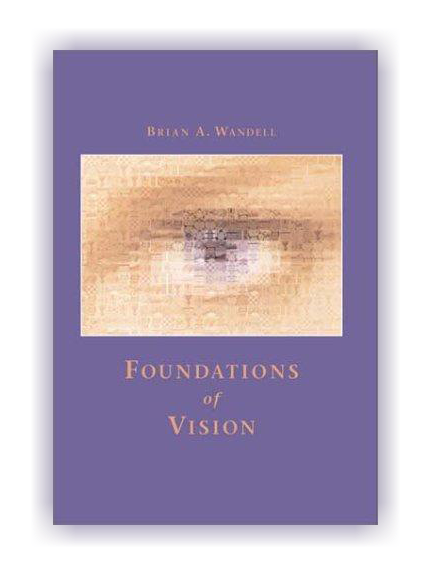
\includegraphics{1995/bookCover/ScannedCover.png}
\end{center}

\bookmarksetup{startatroot}

\chapter{How to study vision}\label{how-to-study-vision-1}

While working to bring this book together, I was inspired and
overwhelmed by the breadth and vibrancy of vision science. Vision
scientists solve problems across the fields of biology, psychology, and
engineering. Our field takes on problems ranging from the nature of
consciousness to the hurry-up-and-ship-it applications needed to keep a
company afloat. In selecting from the huge amount of material available,
I decided to write this book for the student who wishes to know
\emph{how} to study vision. The pages are filled with measurements and
facts; but, my goal in writing this book is to explain to the student
how we learned these facts, not the facts themselves. To organize the
material presented, I have divided the book into three sections. My
division reflects three of the basic problems of vision: encoding,
representation, and interpretation.

\section{Encoding}\label{encoding}

Part One describes how the retinal image is encoded by the visual
pathways. The material in this section is particularly important for
three reasons. First, how the visual system encodes light has
implications for everything else the visual pathways do. Distortions
that are introduced into the signal by poor optics, sparse and uneven
spatial sampling of the image, or meager wavelength encoding become part
of the signal that must be represented and interpreted by the central
visual pathways. We can't understand the central nervous system without
understanding the quality of information encoded within the eye.

Second, the properties of the visual encoding have implications for the
design of instruments that display visual information. The quality of
the representation of pattern and color in display media must be
structured to satisfy, but not exceed, the limits of the human visual
system. For example, the industry of color imaging, including visual
displays, film, and color printing, relies on the fact that human color
vision uses three types of cone photopigments to encode light. As a
result of this sparse representation of wavelength, color reproductions
need not represent the wavelength composition of the original in order
to provide a satisfactory appearance match. This is but one example of
many in which the initial encoding of the image in the human eye defines
practical limits whose properties determine the character of imaging
devices.

Third, the methods and standards of proof that are used to understand
image encoding set an important example concerning the standards of
explanation we aim to achieve at all levels of vision science. The
questions of methods and standards of proof are very important an an
interdisciplinary field like vision science, which draws on expertise
from many different areas. The first section of this book contains
several examples that combine physical calculations, biological
experiments, and behavioral studies. By examining how these fields come
together when we measure the quality of the retinal image formed by the
optics of the eye, and again when we establish that human color vision
is trichromatic, we see how these diverse fields can forge strong links
that define important aspects of visual function. We can learn from
these examples as we move on to other problems in vision science.

\section{Representation}\label{representation}

Part Two of this volume reviews how the encoded image is represented by
the neural response within the peripheral visual pathways. Our
understanding of the neural representation is based on work in several
different disciplines. This section begins with a review of the
anatomical and electrophysiological measurements of the image
representation within the retina and primary visual cortex. These
measurements characterize the neural hardware of the visual
representation and demonstrate that there are several distinct
categories of neurons called \emph{visual streams}. The neurons in these
visual streams respond to light stimulation in differnt ways, and their
signals are communicated to different destinations.

The second half of this section reviews psychological and computational
studies of image representation. The behavioral studies of image
representation involve the simplest performances, such as detection,
discrimination and simple recognition. These experiments have led to
various proposals about how pattern and color information is represented
within the retina and early cortical areas. The computational studies of
image representation cover fundamental issues in efficient image coding
and other image operations.

\section{Interpretation}\label{interpretation}

Perception is an interpretation of the retinal image, not a description.
The third section of this book contains examples of how we interpret the
retinal image to assign perceptual properties such as color, motion, and
shape to objects.

Information in the retinal image may be interpreted in many different
ways. Because we begin with ambiguous information, we cannot make
deducations from the retinal image, only inferences. When we create
algorithms to interpret image data -say, to infer the color, motion, and
shape of objects- we confront the same challenges as the visual
pathways. The success of the visual system in intpreting image data
represents a remarkable achievement.

By studying computations designed to infer object properties, we have
learned that the visual system succeeds in interpreting images because
of statistical regularities present in the visual environment and hence
in the retinal image. These regularities permit the visual system to use
the fragmentary information present in the retinal image to draw
accurate inferences about the physical cause of the image. For example,
when we make inferences from the retinal image, the knowledge that we
live in a three-dimensional world is essential to the correct
interpretation of the image. Often, we are made aware of the existence
of these powerful interpretations and their assumptions when they are in
error, that is, when we discover a visual illusion.

\section{The range of material in this
book}\label{the-range-of-material-in-this-book}

The material I have chosen to include in this book comes from three
sources: theory, data, and fruitful applications that are grounded in
theoretical and empirical vision science. Portions of this book are
written with the expectation that the reader has had some experience
with linear algebra and calculus. In most sections of the book, however,
I have tried to provide the reader with the basic ideas without using
mathematical symbols or formal arguments.

\subsection{Theory}\label{theory}

Certain theoretical and empirical methods appear repeatedly within
vision science. The most important theoretical method, which appears
across all areas of vision science, is linear systems theory. Whether
characterizing optics, neurophysiology, color vision, spatial vision,
image compression, or pattern analysis, linear systems play an important
role. There is little possibility of understanding the current
foundations of vision science without understanding linear systems. I
introduce the principles of linear systems in the first chapter and I
refer to them throughout the book.

Linear methods are not a theory of vision; linear systems methods
consist of a set of experiments that one should use to analyze a system.
If the system's performance satisfies certain experimental properties,
such as the principle of superposition, then we can use linear methods
to characterize the system completely. Even if the system turns out to
be nonlinear, it is useful to begin studying the system using summation
experiments to obtain some insights as to the nature of the
nonlinearities.

A linear characterization of a system is rarely a satisfactory
scientific account of the system. There are usually many theoretical
questions that require further explanation before the scientist is done.
This will be evident in the first section on image encoding. Optical
image formation, photoreceptor sampling and color matching are all
fundamentally linear and thus we can characterize the performance of
these system components. Even when this work is done, we still must
explain the measurements in terms of the purpose of these elements and
how their properties serve the goals of visual perception.

In part, the emphasis on linear systems methods is my choice; in part,
this emphasis is inevitable because of a second choice I made in
selecting the material. I have tried to include important problems that
vision science has solved, or that I think are close to being solved. At
present linear methods are much better understood than nonlinear
methods. Consequently, we understand those problems which yield to
linear analysis much better than we understand nonlinear problems.

A linear characterization of a system is rarely a complete cientific
account of the system. There are usually many theoretical questions that
require further explanation before the scientist is done. This will be
evident in the first section on image encoding. Optical image formation,
photoreceptor sampling, and color matching are all fundamentally linear,
and thus we can characterize the performance of these system components.
However, even when this work is done, we still must expolain the
measurements in terms of the purpose of these elements and how their
properties serve the goals of visual perception.

While linear analyses are central, there are some significant examples
of successful nonlinear analyses. The first example is the analysis of
the relationship between color matching and the cone photocurrent
treatment in Chapter 4. This system consists of an initial linear
encoding followed by a fixed non-linearity. These types of nonlinear
systems can also be treated very thoroughly. The review of pattern
sensitivity, in Chapter 7, also includes models that begin with linear
encodings followed by a nonlinear stage. In the appendix to Chapter 7 I
treat the profoundly nonlinear act of classification. Applications of
Bayesian classification to interpret image data is likely to be a very
important area in the future.

\subsection{Data}\label{data}

The field of vision draws on experimental results from many separate
disciplines, each with its own standards and methods. The tools of
anatomy, electrophysiology, behavior, and computation are so different
that no one can be an expert in all of these disciplines. To be a good
vision scientist, however, one must appreciate the standards and methods
of each discipline. The psychologist must understand whether an
anatomical measurement is sufficiently thorough to serve as a good
standard for comparison in a behavioral experiment; the computational
theorist must understand the generality of a result from
electrophysiology.

I have included empirical studies from all of the disciplines of vision.
I have tried to describe these results, and their theoretical
implications, in enough detail so that the advanced student can learn
something about the standards of each of the fields. By placing these
results together in a single volume I hope to explain what is special
about the interdisciplinary field of vision.

\subsection{Applications}\label{applications}

As I selected problems to review, I did not distinguish strongly between
those that are called basic from those that are called applied. I share
Edwin Land's frustration with this distinction. After a theoretical
lecture on color appearance, Land, who was both a brilliant inventor and
entrepreneur, was asked to explain what applied problem his work would
solve and he replied quickly that the work had a wonderful application.
He then paused while the audience leaned forward to decide whether to
invest in Polaroid stock. If the theory is right, Land whispered
confidentially, we'll finally understand what we are doing.

Vision science finds applications in at least three important areas that
I will draw on throughout the book. The first area is medicine. If we
are to help the blind, we must understand how the visual portion of the
brain functions, including the anatomy and functional properties of
nerve cells. Equally important, we must understand how information is
represented within the brain results in behavior. The results of
behavioral experiments can answer questions about the organization of
information within the visual pathways that are inaccessible to the
anatomist or the electrophysiologist. Together, these results can guide
the development of medical diagnostic tools and prosthetic devices. Tom
Cornsweet's beautiful book, Visual Perception, was a guide to most of my
generation as we first learned about the systematic analysis of the
visual pathways, ranging from the visual pathways to behavior. In this
book I hope to explain to the new student why so many of us found
Cornsweet's presentation exhilirating and to build on Cornsweet's
review.

A second area of application is the design of computer algorithms
capable of analyzing information in an image. Typical applications range
from part inspections in a factory to the identification of a tumor in a
medical image. David Marr's book, Vision, stimulated the interest of
many young scientists in this area. He presented a bold overview that
related biological concepts and computer algorithms of visual
processing. The contrast between the broad scope of Marr's imagination
and the elegant, meticulous discussions by Cornsweet captures something
of the creative tension that can arise when different disciplines
contribute to a broad scientific endeavor.

The third area of application is the design of visual display devices to
communicate information to the human visual system. When two electronic
components communicate, the components must be designed to accommodate a
set of communication protocols. In the case of communication between an
electronic display medium, (e.g.~a television display) and the human
visual system, the designer can only re-design one of the two
components. To communicate information efficiently between the
electronic system and the human visual system, we must build displays
that are matched to human capabilities. A remarkable harmony between
vision science and applications technology has been achieved in some
areas, such as color science. I hope that this book will contribute to
the further coordination of our basic understanding of vision and the
design of useful and efficient visual displays.

\section{A Guide to the Principles of
Vision}\label{a-guide-to-the-principles-of-vision}

Much of vision science is predicated on the principle that the
components of the visual system that limit or govern performance in
various tasks can be quite different. In some experiments performance is
limited by the lens, while in other experiments performance is limited
by a computation in performed in visual cortex. Different visual tasks
may be limited by completely distinct components of the visual pathways.
Hence, a static diagram of the visual pathways, in which zero-crossings
are inexorably followed by a primal sketch, and so forth, with all the
components play the same role across tasks, does not capture the
flexibility and adaptability of the visual pathways.

There are, however, several general principles that I found useful as I
wrote and organized this volume. Some of these principles are embedded
in the organization of the book, repeated in the introductions to the
three sections, and repeated within the chapters themselves. This is the
time, however, to introduce you to the principles, briefly, in one
place.

\subsection{The Inescapable Components of Image
Encoding}\label{the-inescapable-components-of-image-encoding}

The properties of image encoding, such as the blurring by the lens,
receptor sampling, and trichromacy, shape the information available to
the rest of the nervous system. The first third of the book is devoted
to describing these aspects of vision. The properties of image formation
set the stage for what the rest of the nervous system must confront.

The limits of image encoding set limits on the image information
available to the visual pathways. As we shall see, the image encoding is
a very partial description of the light incident at the eye: There is
only a narrow region of high visual acuity in the fovea; the dynamic
range of the sensors is very small; the representation of wavelength is
very coarse. You would never buy a camera with such poor optics and
coarse spatial sampling. Yet, the visual algorithms can interpret the
properties of objects from this poor encoding.

Whether you wish to study the eye, or study algorithms embedded in the
central nervous system, you will not go wrong by studying image encoding
and thinking further about its implications for vision.

\subsection{Adaptation and
Flexibility}\label{adaptation-and-flexibility}

The visual pathways compensate for the poor quality of the image
encoding by their flexibility. Nearly all of the peripheral elements of
the visual pathways adapt in response to the viewing conditions. The
lens accomodates, the strength of the retinal signal varies as the mean
illumination level varies, the eye moves to bring the high visual acuity
portion of the retina into a favorable viewing position. The flexible
responses of the visual system overcome the mediocre image encoding.

The visual system's adjustments, or adaptations, to the environment are
fundamental to its design. We see adaptation throughout the visual
representation, not just in the peripheral components. Because
adaptation is so widespread, it is impossible to characterize the visual
system as a static device. The ability to adapt in response to a
changing environment is a fundamental design principle of the visual
pathways, beginning at the earliest stages. Such adaptation is also an
important property of central brain representations.

\subsection{Image representation: Visual
Streams}\label{image-representation-visual-streams}

As we review the visual representation of the image, we will find that
the neural pathways are organized into several distinct pathways. These
pathways, sometimes called visual streams, can be identified based on
anatomical studies. Some cells have different shapes from others; some
cells send their outputs this way and others send their outputs that
way.

Many of the most important discoveries about vision concern the the
identification of visual streams. Many of the important contemporary
challenges in vision concern explanations of the functional significance
of these streams. Segregation of visual information into these visual
streams begins with the photoreceptors (rods and cones). Clarifications
concerning the visual streams within the optic nerve have revolutionized
our understanding of the visual representation. Understanding the
organization of visual information with respect to these visual streams
is one of most hotly debated topics in modern visual neuroscience.
Identifying new visual streams and understanding their function is an
important challenge to vision scientists.

\subsection{Image interpretation: Statistical
Inferences}\label{image-interpretation-statistical-inferences}

To me, vision science is about how we see things. The interpretations of
the image, or as Helmholtz called them, the unconscious inferences, are
the purpose of vision. I study vision in order to understand the methods
of interpreting images to objects and their properties.

Since the retinal image is often ambiguous, the visual system's success
in interpreting images must be because it makes good assumptions about
the likely properties of objects in the world. Not all configurations of
objects are equally likely; we exist in a three-dimensional world. Not
all surface reflectance functions are equally likely; there are
regularities in the wavelength properties of surfaces and illuminants.
Not all types of motion are equally likely; hard objects cannot pass
through one another. The unequal probabilities of different
interpretations make it possible to make informed guesses about the
color, motion, position and shape of objects. The probabilities of
different events are sufficiently skewed so that the visual system
succeeds at interpreting the image data. Understanding these
regularities, and understanding how to use them to interpret the retinal
image, is central to vision science.

My devotion to image encoding and representation, the first two parts of
this volume, flows from my conviction that we will not understand visual
interpretations of the image without understanding encoding and
representation. The encoding and representation define the environment
in which image interpretation takes place. The encoding and
representation must be structured to permit image interpretation to
succeed. As you look through each section of this volume, you will find
ideas about image interpretation. The material in this book will seem
unified to you if you continue to ask how image encoding and the image
representation serve the ultimate goal of image interpretation.

\part{Image Encoding}

\chapter*{Introduction to Image
Encoding}\label{introduction-to-image-encoding}
\addcontentsline{toc}{chapter}{Introduction to Image Encoding}

\markboth{Introduction to Image Encoding}{Introduction to Image
Encoding}

The first section of this book describes the initial encoding of light
by the eye. Chapter~\ref{sec-image-formation} reviews the image
formation process, that is, the process by which light incident at the
eye is focused onto the retina. Chapter~\ref{sec-photoreceptor-mosaic}
and Chapter~\ref{sec-wavelength-encoding} review the basic properties of
the conversion of light into a neural signal by the light-sensitive
elements of the eye, the \emph{photoreceptors}. This image encoding
establishes essential limits on vision; the consequences of the image
formation process can be found in many parts of the visual neural
representation.

The early chapters introduce and make use of the principles of linear
systems. Linear methods are fundamental to vision science, as they are
to much of science. The well-designed experiment provides a method of
extrapolating beyond the experimental measurements, and linear systems
methods provide such a method. A notion of how to extrapolate beyond the
experimental measurements is necessary because we can rarely measure the
response to every important stimulus. The significance of linear systems
methods is that they permit us to evaluate whether we can use the
response to a few stimuli to predict the responses to other stimuli.

Since the linear methods apply well to image formation, it seems natural
to introduce linear systems as a solution to the problem of measuring
the properties of eye. The principles come up again in multiple
sections, including analyses of the properties of color, pattern, and
motion perception. Thus the reader will have several opportunities to
see the application of these ideas.

Since the first edition of this book, new technologies to measure image
encoding, and new facts about the image encoding, have been discovered.
A particularly impactful technology, adaptive optics, has enabled
measurements in the living human eye that were not possible at the time
of the 1st edition. In this edition I explain the principles of adaptive
optics and describe how it is used both to measure the properties of
image formation and to use this knowledge to deliver stimuli with
remarkable precision.

In addition, a new class of photosensitive cells was discovered. These
cells are not photoreceptors, rather they are ganglion cells that
contain a light sensitive pigment distributed across their entire
extent. The discovery of these intrinsically photosensitive retinal
ganglion cells (ipRGCs) is an important development with implications
for vision and other behaviors that depend on light sensitivity.

Finally, this 2nd edition is more firmly connected to computational
methods. As we introduce many of the concepts of optics and encoding, we
provide the reader with a set of software methods that can be used to
calculate the encoding and responses quantitatively.

\section*{Image formation}\label{image-formation}
\addcontentsline{toc}{section}{Image formation}

\markright{Image formation}

The quality and general properties of the image formed at the retina
establish the basic image parameters that the rest of the nervous system
must use to make inferences about objects. Because the image formation
process is linear, we can characterize its properties fairly thoroughly.
Measurements from the eye show that even when optical focus is at its
best, the image of a point is spread across eight or more
photoreceptors. It follows that the image formation process attenuates
the contrast of patterns that vary rapidly across space. This leaves the
nervous system with only a small contrast range available in the fine
spatial detail of an image, while there is a substantial contrast range
present in slowly varying spatial patterns. Finally, the precise meaning
of high and low frequency varies with the wavelength of the incident
light because the quality of the retinal image varies strongly with
wavelength. Under ordinary viewing conditions the short wavelength light
(blue portion of the spectrum) is blurred strongly so that very little
pattern information is available in this part of the spectrum compared
to longer wavelengths of light (green, yellow and red parts of the
spectrum).

\section*{The Spatial Mosaic of
Photoreceptors}\label{the-spatial-mosaic-of-photoreceptors}
\addcontentsline{toc}{section}{The Spatial Mosaic of Photoreceptors}

\markright{The Spatial Mosaic of Photoreceptors}

Chapter~\ref{sec-photoreceptor-mosaic} reviews the spatial arrangement
of the light-sensitive elements of the photoreceptors. There are two
fundamentally different types of receptors, the rods and cones. The
spatial organization of the rod and cone photoreceptor mosaics differ;
each mosaic reflects the main goal of the visual stream it initiates.

The rod visual stream initiates vision under low illumination conditions
when relative few quanta are available. The rods are present in high
density to capture more quanta, not to achieve high spatial resolution.
Indeed, the spatial resolution of the rod pathway is fairly coarse since
the outputs of many rod photoreceptors converge onto single retinal
cells.

The visual streams initiated by the cone mosaic ordinarily operate at
high light levels where there are plenty of quanta. The organization of
the cone mosaic can be understood in terms of the goal of representing
fine spatial detail rather than capturing more quanta. This goal is
reflected separately in the spatial arrangement of the separate mosaics
of the three different types of cones, the \(L\), \(M\), and \(S\)
cones. The density of the short-wavelength sensitive \(S\) cones is
lowest, matching the poor resolution of the optics in the
short-wavelength region. Only the \(L\) and \(M\) cones are present in
the very central fovea, where they have a very high sampling density and
form a locally regular sampling grid. The sampling density of the \(L\)
and \(M\) cones is also a good match to the quality of the image passed
by the optics of the eye in the portion of the wavelength spectrum where
they have their peak sensitivity. Signals from individual cones in the
fovea do not converge onto retinal neurons, but instead these signals
are communicated along private neural channels to the cortex.

\section*{Wavelength Encoding}\label{wavelength-encoding}
\addcontentsline{toc}{section}{Wavelength Encoding}

\markright{Wavelength Encoding}

Chapter~\ref{sec-wavelength-encoding} reviews how the visual pathways
encode the wavelength of light, a process that greatly influences color
appearance. The behavioral predictions that the eye contains three types
of cones, as well as behavioral predictions of the way these cones
encode wavelength, have been confirmed in a stunning set of experiments
that represent an intellectual collaboration between very different
disciplines. The nexus of results from physics, psychology, and biology
concerning wavelength encoding form one of most beautiful and satisfying
stories in science. The successful interactions between these
disciplines is a remarkable intellectual achievement. The facts
concerning how the visual pathways encode wavelength has been important
for all color imaging technologies. The scientific methods that link the
color matching experiment to the cone photocurrents are important for
all of us who wish to relate behavior and brain.

\chapter{Image Formation}\label{sec-image-formation}

\section{Image Formation Overview}\label{image-formation-overview}

The cornea and lens are the interface between the physical world of
light and the visual encoding. The cornea and lens bring light into
focus at the light sensitive receptors in the retina. These cells
initiate a series of visual events that result in our visual experience.

The initial encoding of light at the retina is but the first in a series
of visual transformations: The stimulus incident at the cornea is
transformed into an image at the retina. The retinal image is
transformed into a neural response by the light sensitive elements of
the eye, the photoreceptors. The photoreceptor responses are transformed
to a neural response on the optic nerve. The optic nerve representation
is transformed into a cortical representation, and so forth. We can
describe most of our understanding of these transformations, and thus
most of our understanding of the early encoding of light by the visual
pathways by using linear systems theory. Because all of our visual
experience is limited by the image formation within our eye, we begin by
describing this transformation of the light signal and we will use this
analysis as an introduction to linear methods.

\section{Optical Components of the Eye}\label{sec-optical-components}

\begin{figure}

\centering{

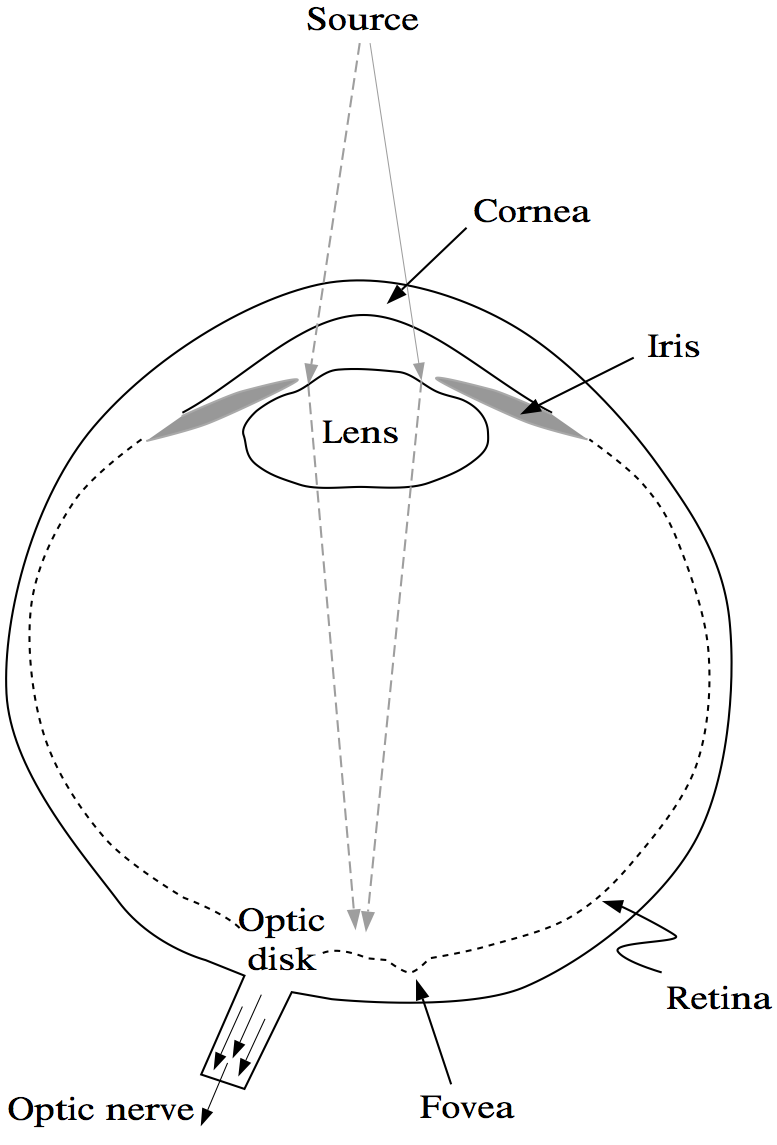
\includegraphics[width=0.4\textwidth,height=\textheight]{wp-content/uploads/2012/02/eyeball.png}

}

\caption{\label{fig-eyeball}The image formation components of the eye.
The cornea and lens focus the image onto the retina. The cornea
initiates the bending of the light rays from the source. The rays must
pass through the pupil which is bordered by the iris. The flexible lens
then further bends the rays. In this image, the rays are focused near
the fovea, a region that is specialized for high visual acuity. The
retinal output fibers come together to form a bundle that exits through
a hole in the retina at the optic disk (or blindspot). The fiber bundle
is the optic nerve.}

\end{figure}%

Figure~\ref{fig-eyeball} contains an overview of the imaging components
of the eye. Light from a source arrives at the cornea and is focused by
the cornea and lens onto the photoreceptors, a collection of light
sensitive neurons. The photoreceptors are part of a thin layer of neural
tissue, called the retina. The photoreceptor signals are communicated
through the several layers of retinal neurons to the neurons whose
output fibers makes up the optic nerve. The optic nerve fibers exit
through a hole in the retina called the optic disk. The optical imaging
of light incident at the cornea into an image at the retinal
photoreceptors is the first visual transformation. Since all of our
visual experiences are influenced by this transformation, we begin the
study of vision by analyzing the properties of image formation.

When we study transformations, we must specify their inputs and outputs.
As an example, we will consider how simple one-dimensional intensity
patterns displayed on a video display monitor are imaged onto the retina
(Figure~\ref{fig-imgfor-monitor-retina} (a)). In this case the input is
the light signal incident at the cornea. One-dimensional patterns have a
constant intensity along the, say, horizontal dimension and varies along
the perpendicular (vertical) dimension. We will call the pattern of
light intensity we measure at the monitor screen the monitor image. We
can measure the intensity of the one-dimensional image by placing a
light-sensitive device called a photodetector at different positions on
the screen. The vertical graph in Figure~\ref{fig-imgfor-monitor-retina}
(b) shows a measurement of the intensity of the monitor image at all
screen locations.

The output of the optical transformation is the image formed at the
retina. When the input image is one-dimensional, the retinal image will
be one-dimensional, too. Hence, we can represent it using a curve as in
Figure~\ref{fig-imgfor-monitor-retina} (c). We will discuss the optical
components of the visual system in more detail later in this chapter,
but from simply looking at a picture of the eye in
Figure~\ref{fig-eyeball} we can see that the monitor image passes
through a lot of biological material before arriving at the retina.
Because the optics of the eye are not perfect, the retinal image is not
an exact copy of the monitor image: The retinal image is a blurred copy
of the input image.

The image in Figure~\ref{fig-imgfor-monitor-retina} (b) shows one
example of an infinite array of possible input images. Since there is no
hope of measuring the response to every possible input, to characterize
optical blurring completely we must build a model that specifies how any
input image is transformed into a retinal image. We will use linear
systems methods to develop a method of predicting the retinal image from
any input image.

\begin{figure}

\centering{

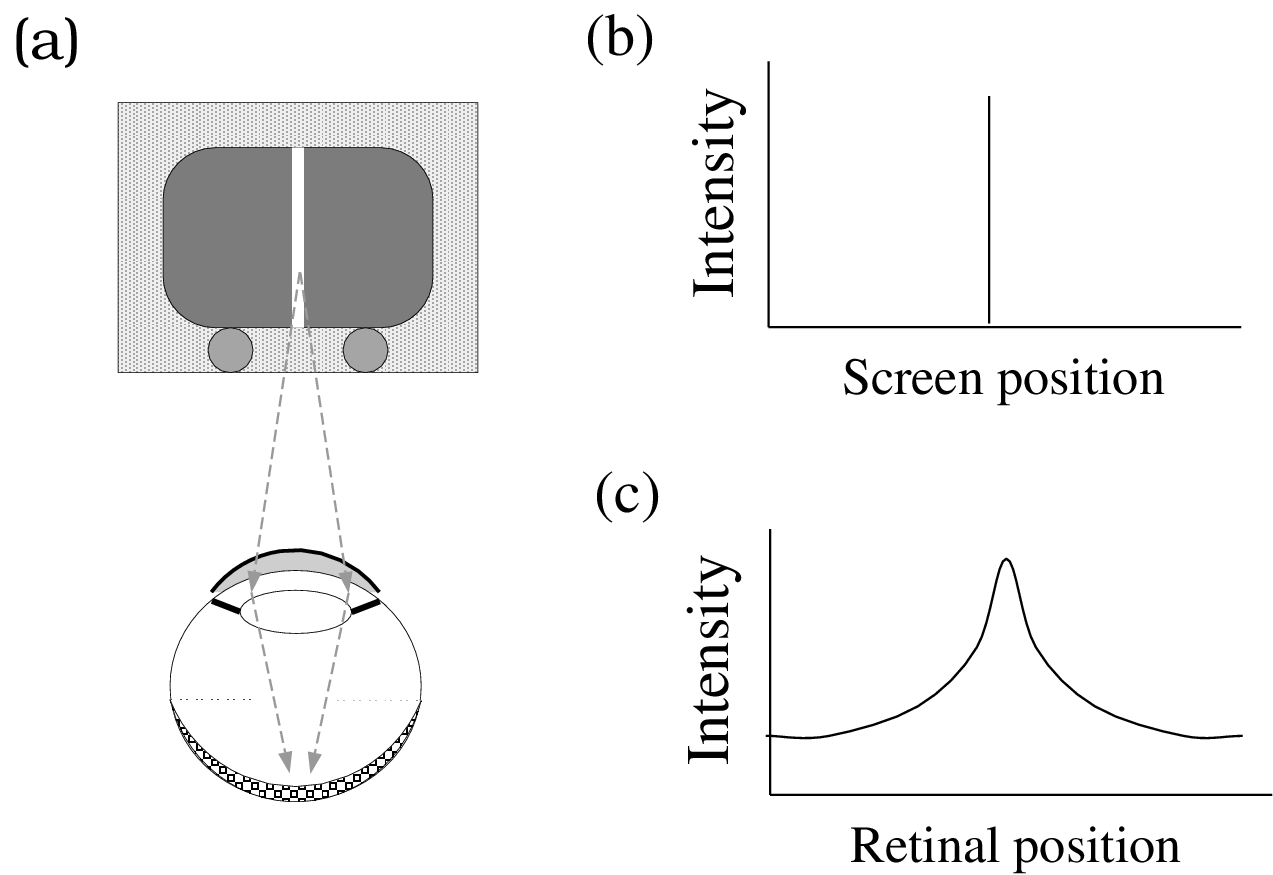
\includegraphics[width=0.6\textwidth,height=\textheight]{wp-content/uploads/2012/02/monitor.to_.retina1.png}

}

\caption{\label{fig-imgfor-monitor-retina}Retinal image formation
illustrated with a single-line input image. (a) A one-dimensional
monitor image consists of a set of lines at different intensities. The
image is brought to focus on the retina by the cornea and lens. (b) We
can represent the intensity of a one-dimensional image using a simple
graph that shows the light as a function of horizontal screen position.
Only a single value is plotted since the one-dimensional image is
constant along the vertical dimension. (c) The retinal image is a
blurred version of the one-dimensional input image. The retinal image is
also one-dimensional and is also represented by a single
curve.monitor.to.retina}

\end{figure}%

\section{Reflections From the Eye}\label{reflections-from-the-eye}

To study the optics of a human eye you will need an experimental eye, so
you might invite a friend to dinner. In addition, you will need a light
source, such as a candle, as a stimulus to present to your friend's eye.
If you look directly into your friend's eye, you will see a mysterious
darkness that has beguiled poets and befuddled visual scientists. The
reason for the darkness can be understood by considering the problem of
ophthalmoscope design illustrated in
Figure~\ref{fig-imgfor-opthalmoscope}(a).

\begin{figure}

\centering{

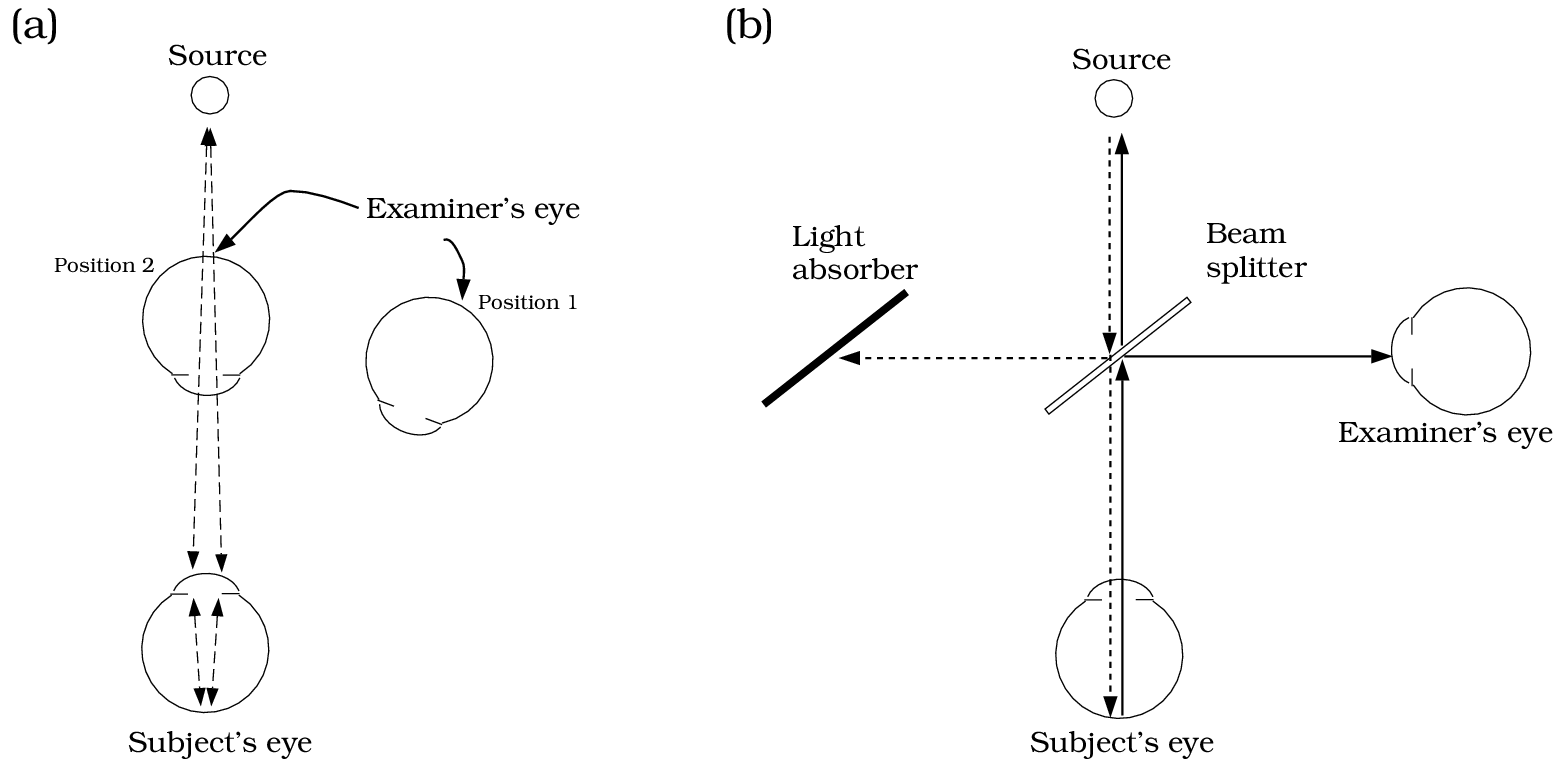
\includegraphics[width=0.7\textwidth,height=\textheight]{wp-content/uploads/2012/02/ophthalmoscope2.png}

}

\caption{\label{fig-imgfor-opthalmoscope}An ophthalmoscope is used to
see an image reflected from the interior of the eye. (a) When we look
directly into the eye, we cast a shadow making it impossible to see
light reflected from the interior of the eye. (b) The ophthalmoscope
permits us to see light reflected from the interior of the eye.
Helmholtz invented the first ophthalmoscope. (After Cornsweet (1970))}

\end{figure}%

If the light source is behind you, so that your head is between the
light source and the eye you are studying, then your head will cast a
shadow that interferes with the light from the point source arriving at
your friend's eye. As a result, when you look in to measure the retinal
image you see nothing beyond what is in your heart. If you move to the
side of the light path, the image at the back of your friend's eye will
be reflected towards the light source, following a reversible path.
Since you are now on the side, out of the path of the light source, no
light will be sent towards your eye.

\begin{figure}

\centering{

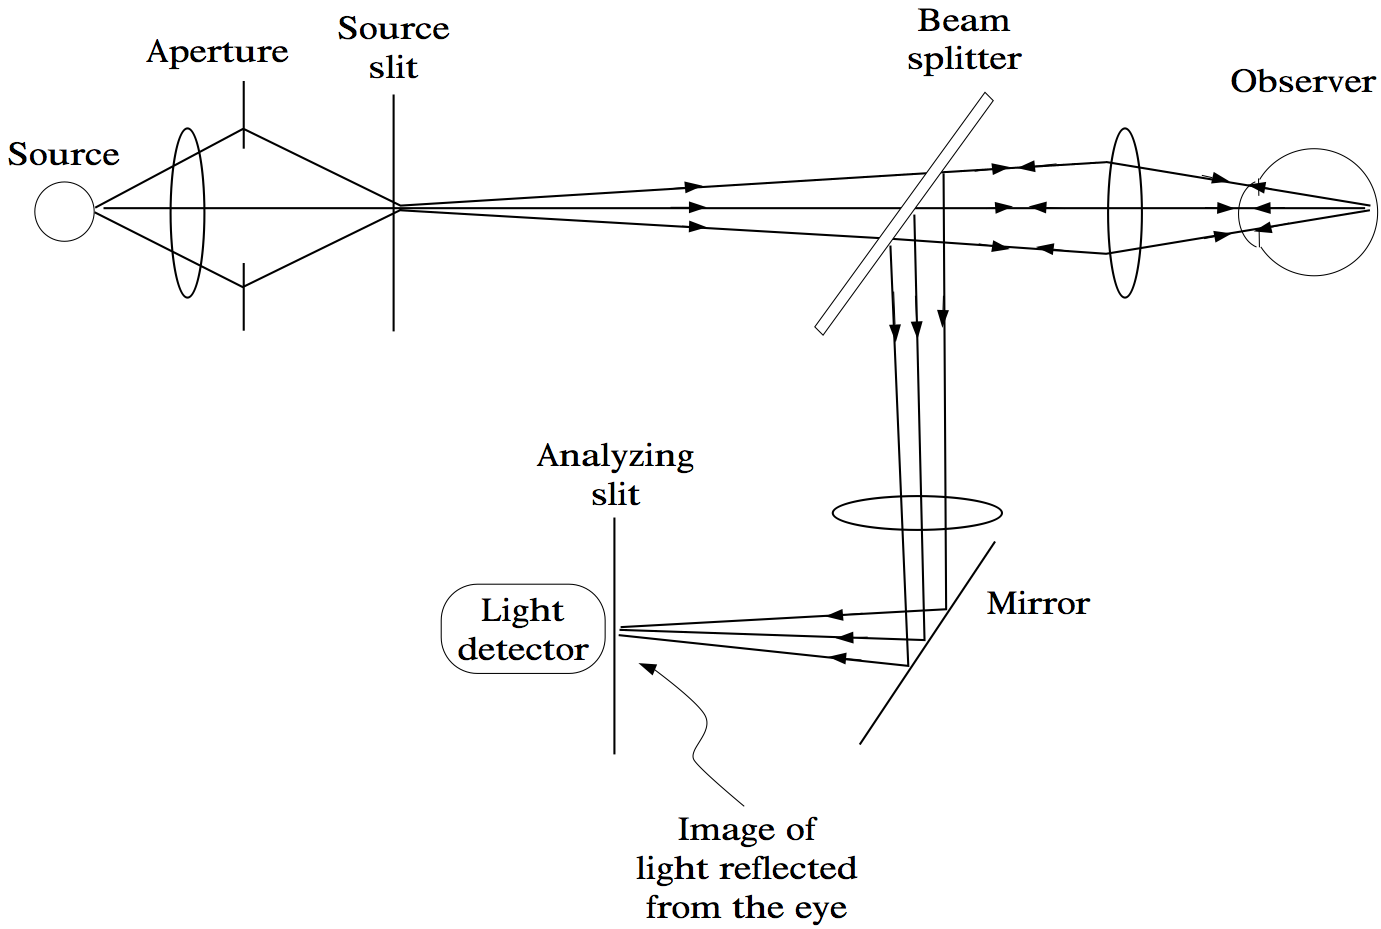
\includegraphics[width=0.8\textwidth,height=\textheight]{wp-content/uploads/2012/02/cg.apparatus1.png}

}

\caption{\label{fig-imgfor-cgapparatus}A modified opthalmoscope measures
the human retinal image. Light from a bright source passes through a
slit and into the eye. A fraction of the light is reflected from the
retina and is imaged. The intensity of the reflected light is measured
at dif- ferent spatial positions by varying the location of the
analyzing slit. (After Campbell and Gubisch (1966), Fig. 2)}

\end{figure}%

Flamant (1955) first measured the retinal image using a modified
ophthalmoscope. She modified the instrument by placing a light sensitive
recording, a photodetector, at the position normally reserved for the
ophthalmologist's eye. In this way, she measured the intensity pattern
of the light reflected from the back of the observer's eye. Campbell and
Gubisch (1966) used Flamant's method to build their apparatus, which is
sketched in Figure~\ref{fig-imgfor-cgapparatus}. Campbell and Gubisch
measured the reflection of a single bright line, that served the input
stimulus in their experiment. As shown in the figure, a beam-splitter
placed between the input light and the observer's eye divides the input
stimulus into two parts. The beam-splitter causes some of the light to
be turned away from the observer and lost; this stray light is absorbed
by a light baffle. The rest of the light continues toward the observer.
When the light travels in this direction, the beam-splitter is an
annoyance, serving only to lose some of the light; it will accomplish
its function on the return trip.

\begin{figure}

\centering{

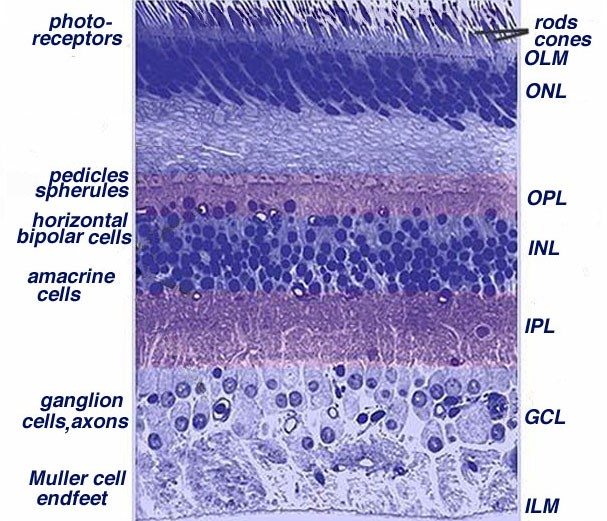
\includegraphics[width=0.6\textwidth,height=\textheight]{wp-content/uploads/2012/02/knolb2012retinasection.jpeg}

}

\caption{\label{fig-imgfor-retinalcross}The retina contains the light
sensitive photoreceptors where light is focussed. This cross-section of
a monkey retina outside the fovea shows there are several layers of
neurons in the optical path between the lens and the photoreceptors. As
we will see later, in the central fovea these neurons are displaced to
leaving a clear optical path from the lens to the photoreceptors
(Source: Kolb et al. (2011)).}

\end{figure}%

The light that enters the observer's eye is brought to a good focus on
the retina by a lens. A small fraction of the light incident on the
retina is reflected and passes -- a second time -- through the optics of
the eye. On the return path of the light, the beam-splitter now plays
its functional role. The reflected image would normally return to a
focus at the light source. But the beam-splitter divides the returning
beam so that a portion of it is brought to focus in a measurement plane
to one side of the apparatus. Using a very fine slit in the measurement
plane, with a photodetector behind it, Campbell and Gubisch measured the
reflected light and used the measurements of the reflected light to
infer the shape of the image on the retinal surface.

What part of the eye reflects the image? In
Figure~\ref{fig-imgfor-retinalcross} we see a cross-section of the
peripheral retina. In normal vision, the image is focused on the retina
at the level of the photoreceptors. The light measured by Campbell and
Gubisch probably contains components from several different planes at
the back of the eye. Thus, their measurements probably underestimate the
quality of the image at the level of the photoreceptors
Figure~\ref{fig-imgfor-cg-data} shows several examples of Campbell and
Gubisch's measurements of the light reflected from the eye when the
observer is looking at a very fine line. The different curves show
measurements for different pupil sizes. When the pupil was wide open
(top, 6.6mm diameter) the reflected light is blurred more strongly than
when the pupil is closed (middle, 2.0mm). Notice that the measurements
made with a large pupil opening are less noisy; when the pupil is wide
open more light passes into the eye and more light is reflected,
improving the quality of the measurements. The light measured in
Figure~\ref{fig-imgfor-cg-data} passed through the optical elements of
the eye twice, while the retinal image passes through the optics only
once. It follows that the spread in these curves is wider than the
spread we would observe had we measured at the retina. How can we use
these doublepass measurements to estimate the blur at the retina? To
solve this problem, we must understand the general features of their
experiment. It is time for some theory.

\begin{figure}

\centering{

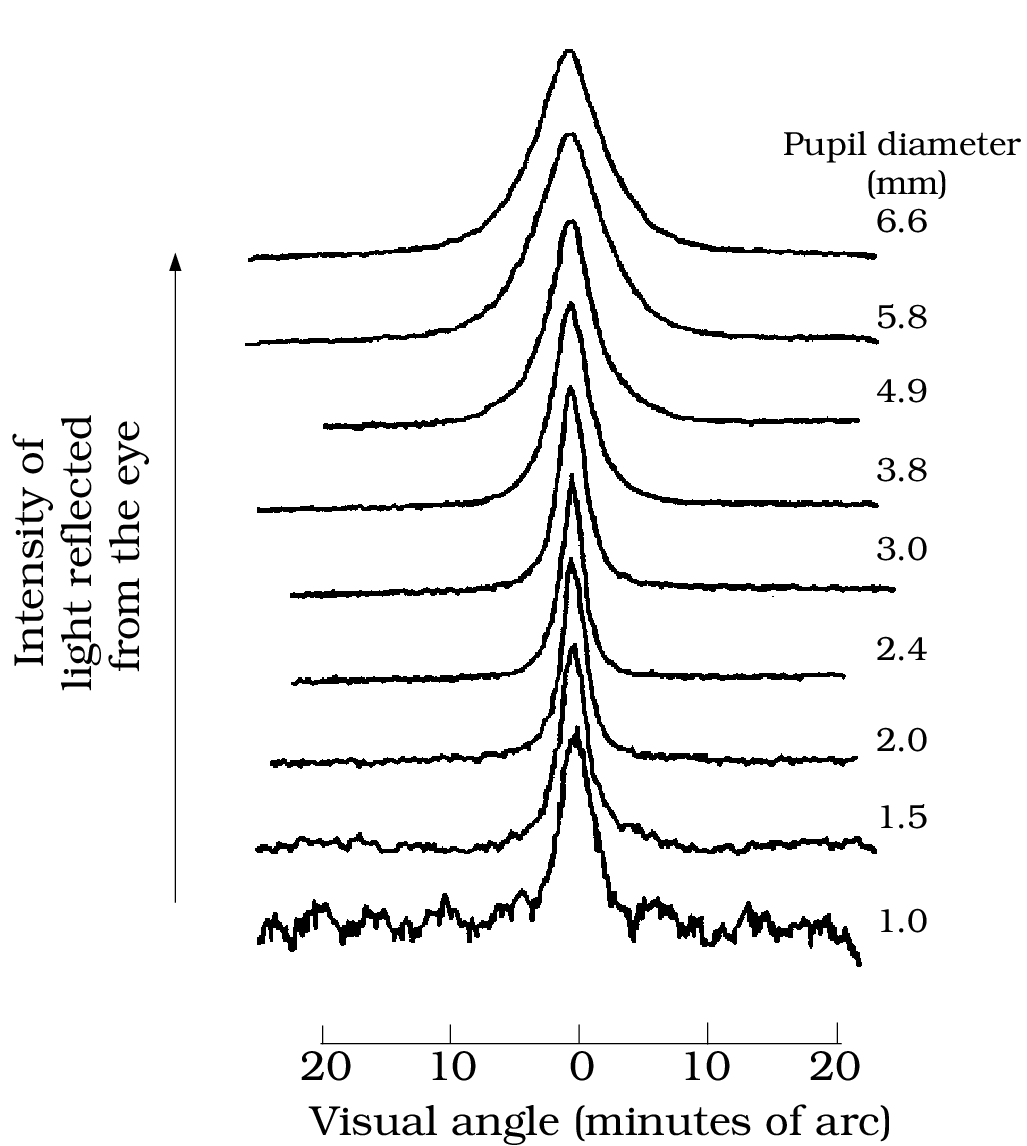
\includegraphics[width=0.6\textwidth,height=\textheight]{wp-content/uploads/2012/02/cg.data_.png}

}

\caption{\label{fig-imgfor-cg-data}Experimental measurements of light
that has been reflected from a human eye looking at a fine line. The
reflected light has been blurred by double passage through the optics of
the eye. (Source: Campbell and Gubisch (1966)).}

\end{figure}%

\section{Linear Systems Methods}\label{linear-systems-methods}

A good theoretical account of a transformation, such as the mapping from
monitor image to retinal image, should have two important features.
First, the theoretical account should suggest to us which measurements
we should make to characterize the transformation fully. Second, the
theoretical account should tell us how to use these measurements to
predict the retinal image distribution for all other monitor images.

In this section we will develop a set of general tools, referred to as
linear systems methods. These tools will permit us to solve the problem
of estimating the optical transformation from the monitor to the retinal
image. The tools are sufficiently general, however, that we will be able
to use them repeatedly throughout this book.

There is no single theory that applies to all measurement situations.
But, linear systems theory does apply to many important experiments.
Best of all, we have a simple experimental test that permits us to
decide whether linear systems theory is appropriate to our measurements.
To see whether linear systems theory is appropriate, we must check to
see that our data satisfy the two properties of homogeneity and
superposition.

\subsection{Homogeneity}\label{homogeneity}

\begin{figure}

\centering{

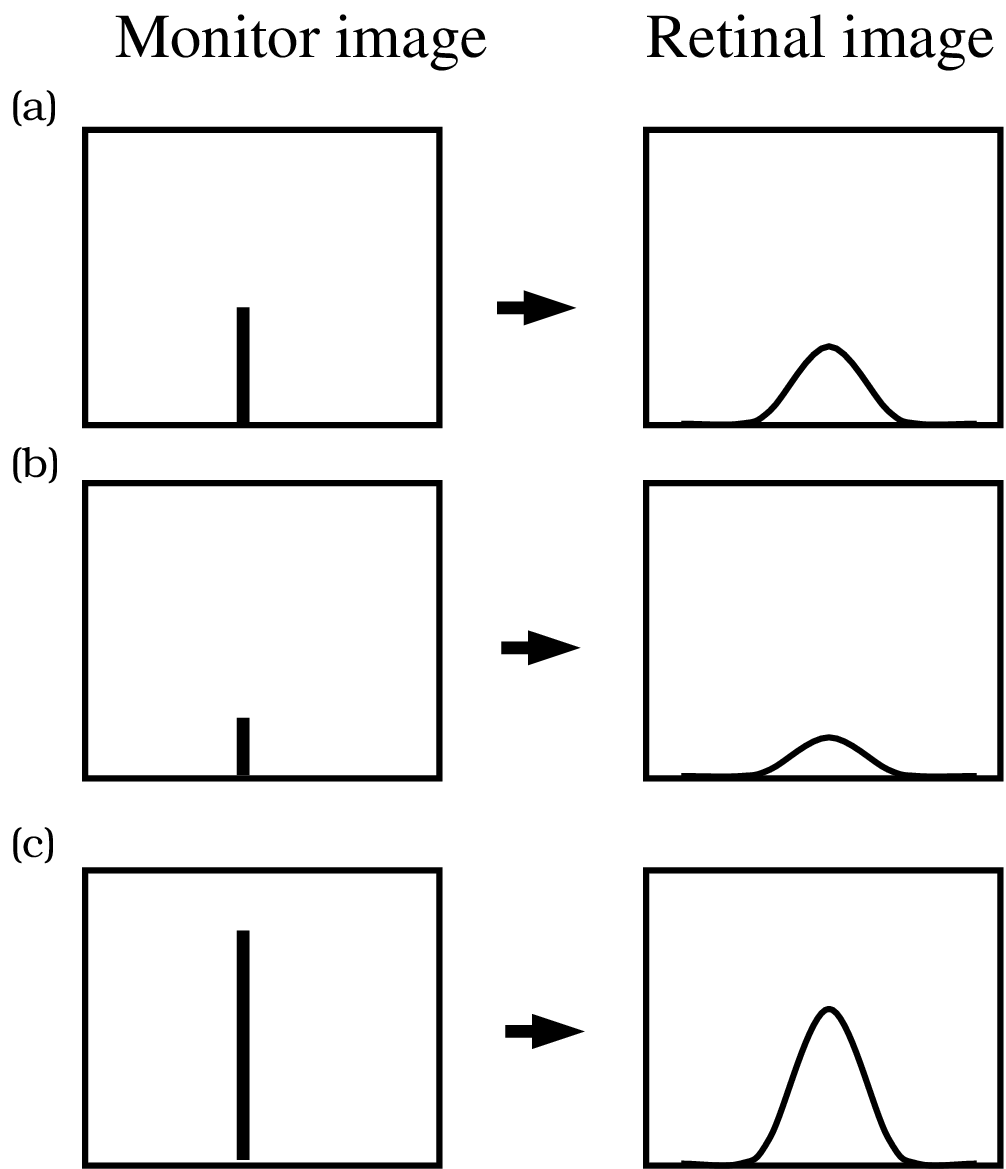
\includegraphics[width=0.4\textwidth,height=\textheight]{wp-content/uploads/2012/02/homogeneity.png}

}

\caption{\label{fig-imgfor-homogeneity}The principle of homogeneity. An
input stimulus and corresponding retinal image are shown in each part of
the figure. The three input stimuli are the same except for a scale
factor. Homogeneity is satisfied when the corresponding retinal images
are scaled by the same factor. Part (a) shows an input image at unit
intensity, while (b) and (c) show the image scaled by 0.5 and 2.0
respectively}

\end{figure}%

A test of \emph{homogeneity} is illustrated in
Figure~\ref{fig-imgfor-homogeneity}. The left-hand panels show a series
of monitor images, and the right-hand panels show the corresponding
measurements of reflected light. Suppose we represent the intensities of
the lines in the one-dimensional monitor image using the vector
\(\boldsymbol{p}\) (upper left) and we represent the retinal image
measurements by the vector \(\boldsymbol{r}\). Now, suppose we scale the
input signal by a factor \(a\), so that the new input is
\(a \boldsymbol{p}\). We say that the system satisfies homogeneity if
the output signal is also scaled by the same factor of \(a\), and thus
the new output is \(a \boldsymbol{r}\). For example, if we halve the
input intensity, then the reflected light measured at their
photodetector should be one-half the intensity (middle panel). If we
double the light intensity, the response should double (bottom panel).
Campbell and Gubisch's measurements of light reflected from the human
eye satisfy homogeneity.

\begin{tcolorbox}[enhanced jigsaw, left=2mm, colframe=quarto-callout-note-color-frame, bottomtitle=1mm, title=\textcolor{quarto-callout-note-color}{\faInfo}\hspace{0.5em}{Vector notation}, opacitybacktitle=0.6, colbacktitle=quarto-callout-note-color!10!white, toprule=.15mm, arc=.35mm, coltitle=black, leftrule=.75mm, breakable, colback=white, toptitle=1mm, titlerule=0mm, rightrule=.15mm, opacityback=0, bottomrule=.15mm]

We will use vectors and matrices in our calculations to eliminate
burdensome notation. Matrices will be denoted by boldface, upper case
Roman letters, \(\mathbf{M}\). Column vectors will be denoted using
lower case boldface Roman letters, \(\mathbf{v}\). The transpose
operation will be denoted by a superscript \(T\), \(\mathbf{v}^T\).
Scalar values will be in normal typeface, and they will usually be
denoted using Roman characters (\(a\)) except when tradition demands the
use of Greek symbols (\(\alpha\)). The \(i^{th}\) entry of a vector,
\(\mathbf{v}\), is a scalar and will be denoted as \(v_i\). The
\(i^{th}\) column of a matrix, \(\mathbf{M}\), is a vector that we
denote as \(\mathbf{m}_i\). The scalar entry in the \(i^{th}\) row and
\(j^{th}\) column of the matrix \(\mathbf{M}\) will be denoted
\(m_{ij}\).

\end{tcolorbox}

\subsection{Superposition}\label{superposition}

\emph{Superposition}, used as both an experimental procedure and a
theoretical tool, is probably the single most important idea in this
book. You will see it again and again in many forms. We describe it here
for the first time.

\begin{figure}

\centering{

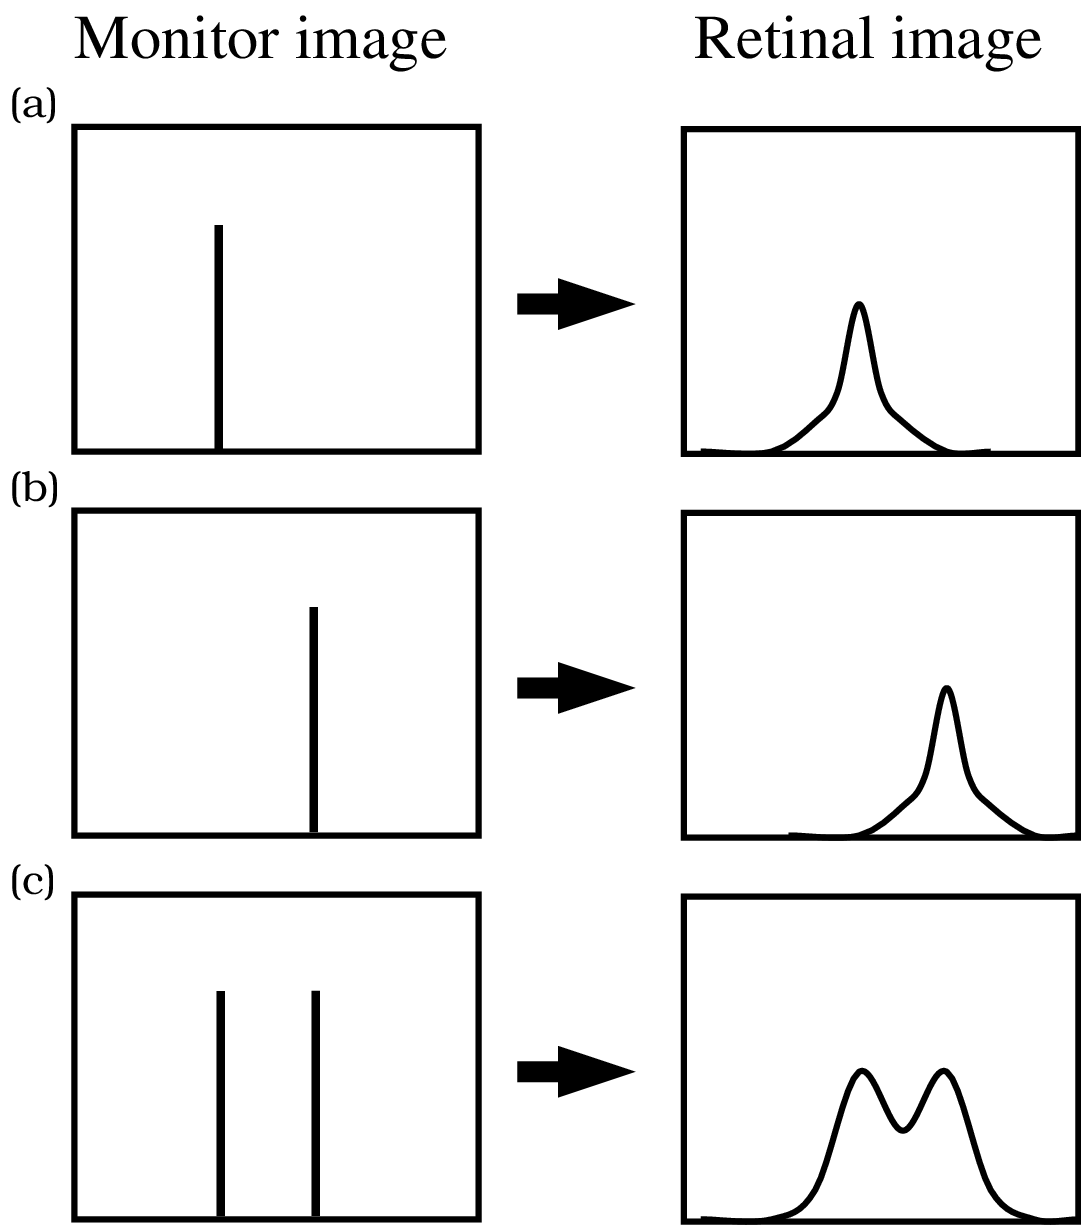
\includegraphics[width=0.5\textwidth,height=\textheight]{wp-content/uploads/2012/02/superposition.png}

}

\caption{\label{fig-imgfor-superposition}The principle of superposition.
Each of the three parts of the picture shows an input stimulus and the
corresponding retinal image. The stimulus in part (a) is a single-line
image and in part (b) the stimulus is a second line displaced from the
first. The stimulus in part (c) is the sum of the first two lines.
Superposition holds if the retinal image in part (c) is the sum of the
retinal images in parts (a) and (b).}

\end{figure}%

Suppose we measure the response to two different input stimuli. For
example, suppose we find that input pattern \(\boldsymbol{p}\) (top
left) generates the response \(\boldsymbol{r}\) (top right), and input
pattern \(\boldsymbol{p}'\) (middle left) generates response
\(\boldsymbol{r}'\) (middle right). Now we measure the response to a new
input stimulus equal to the sum of \(\boldsymbol{p}\) and
\(\boldsymbol{p}'\). If the response to the new stimulus is the sum of
the responses measured singly, \(\boldsymbol{r} + \boldsymbol{r}'\),
then the system is a \emph{linear system}. By measuring the responses to
stimuli individually and then the response to the sum of the stimuli, we
test superposition. When the response to the sum of the stimuli equals
the sum of the individual responses, then we say the system satisfies
superposition. Campbell and Gubisch's measurements of light reflected
from the eye satisfy this principle.

We can summarize homogeneity and superposition succinctly using two
equations. Write the linear optical transformation that maps the input
image to the light intensity at each of the receptors as

\begin{equation}\phantomsection\label{eq-linear-transform}{
\mathbf{r} = L(\mathbf{p})
}\end{equation}

Homogeneity and superposition are defined by the pair of equations:

\begin{equation}\phantomsection\label{eq-homogeneity}{
L(a,\mathbf{p}) = a ~ L(\mathbf{p}) \quad \text{(Homogeneity)} 
}\end{equation} \begin{equation}\phantomsection\label{eq-superposition}{
L(\mathbf{p} + \mathbf{p}') = L(\mathbf{p}) + L(\mathbf{p}') \quad \text{(Superposition)}
}\end{equation}

\subsection{Implications of Homogeneity and
Superposition}\label{implications-of-homogeneity-and-superposition}

Figure~\ref{fig-imgfor-homsup} illustrates how we will use linear
systems methods to characterize the relationship between the input
signal from a monitor, light reflected from the eye (we analyze a
one-dimensional monitor image to simplify the notation. The principles
remain the same, but the notation becomes cumbersome when we consider
two-dimensional images.). First, we make an initial set of measurements
of the light reflected from the eye for each single-line monitor image,
with the line set to unit intensity. If we know the images from
single-line images, and we know the system is linear, then we can
calculate the light reflected from the eye from any monitor image: Any
one-dimensional image is the sum of a collection of lines.

\begin{figure}

\centering{

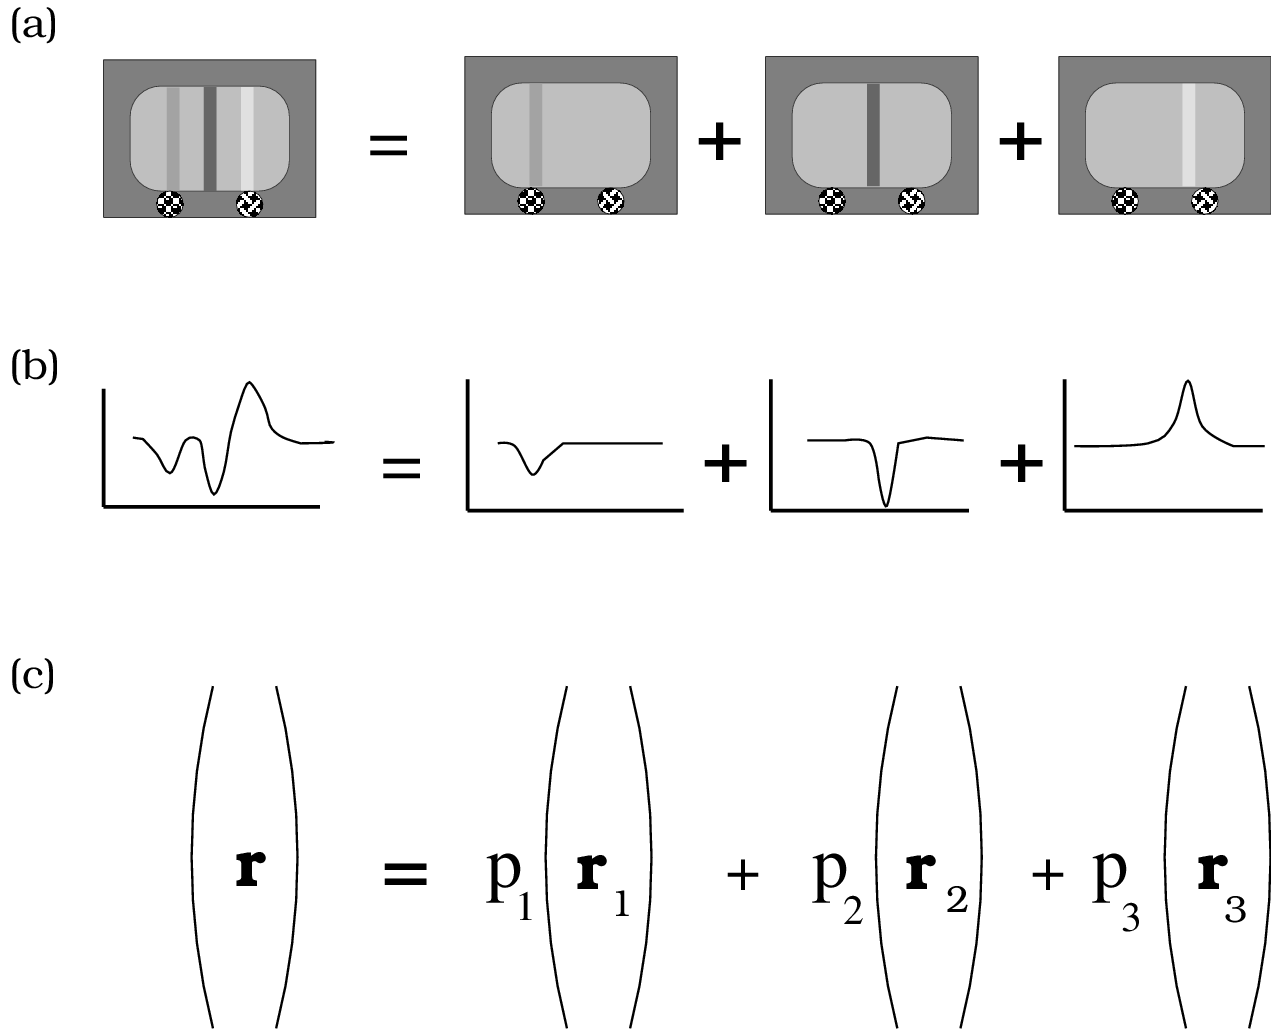
\includegraphics[width=0.5\textwidth,height=\textheight]{wp-content/uploads/2012/02/app.hom_.sup_1.png}

}

\caption{\label{fig-imgfor-homsup}A one-dimensional monitor image is the
weighted sum of a set of lines. An example of a one-dimensional image is
shown on the left and the individual monitor lines comprising the
monitor image are shown separately on the right. (b) Each line in the
component monitor image contributes to the retinal image. The retinal
images created by the individual lines are shown below the individual
monitors. The sum of the retinal images is shown on the left. (c) The
retinal image generated by the \$i\^{}\{th\} monitor line at unit
intensity is \(\mathbf{r}_i\). The intensity of the \(i\text{th}\)
monitor line is \(p_i\). By homogeneity, the retinal image of the
\(i^{th}\) monitor line is \(p_i \mathbf{r}_i\). By superposition, the
retinal image of the collection of mointor lines is the sum of the
individual retinal images, \(\sum_{i} p_i \mathbf{r}_i\)}

\end{figure}%

Consider an arbitrary one-dimensional image, as illustrated at the top
of Figure~\ref{fig-imgfor-homsup}. We can conceive of this image as the
sum of a set of single-line monitor images, each at its own intensity,
\(p_i\). We have measured the reflected light from each single-line
image alone, call this \(\mathbf{r}_i\) for the \(i^{th}\) line. By
homogeneity it follows that the reflected light from the \(i^{th}\) line
will be a scaled version of this response, namely \(p_i \mathbf{r}_i\).
Next, we combine the light reflected from the single-line images. By
superposition, we know that the light reflected from the original
monitor image, \(\mathbf{r}\), is the sum of the light reflected from
the single-line images,

\begin{equation}\phantomsection\label{eq-weighted-sum}{
\mathbf{r} = \sum_{i}^{N} p_i \mathbf{r}_i .
}\end{equation}

Equation~\ref{eq-weighted-sum} defines a transformation that maps the
input stimulus, \(\boldsymbol{p}\), into the measurement,
\(\boldsymbol{r}\). Because of the properties of homogeneity and
superposition, the transformation is the weighted sum of a fixed
collection of vectors: When the monitor image varies, only the weights
in the formula, \(p_i\), vary but the vectors \(\boldsymbol{r}_i\), the
reflections from single-line stimuli, remain the same. Hence, the
reflected light will always be the weighted sum of these reflections.

To represent the weighted sum of a set of vectors, we use the
mathematical notation of \emph{matrix multiplication}. Multiplying a
matrix times a vector computes the weighted sum of the matrix columns;
the entries of the vector define the weights. Matrix multiplication and
linear systems methods are closely linked. In fact, the set of all
possible matrices define the set of all possible linear transformations
of the input vectors.

Matrix multiplication has a shorthand notation to replace the explicit
sum of vectors in Equation~\ref{eq-weighted-sum}. In the example here,
we define a matrix, \(\mathbf{R}\), whose columns are the responses to
individual monitor lines at unit intensity, \(\mathbf{r}_i\). The matrix
\(\mathbf{R}\) is called the system matrix. Matrix multiplication of the
input vector, \(\mathbf{p}\), times the system matrix \(\mathbf{R}\),
transforms the input vector into the output vector. Matrix
multiplication is written using the notation

\begin{equation}\phantomsection\label{eq-matrix-mult}{
\mathbf{r} = \mathbf{R} \mathbf{p}
}\end{equation}

Matrix multiplication follows naturally from the properties of
homogeneity and superposition. Hence, if a system satisfies homogeneity
and superposition, we can describe the system response by creating a
\emph{system matrix} that transforms the input to the output.

\subsection{Why Linear Methods are
Useful}\label{why-linear-methods-are-useful}

Let's use a specific numerical example to illustrate the principle of
matrix multiplication. This will also help explain why the method is so
useful.

Suppose we measure a monitor that displays only three lines. We can
describe the monitor image using a column vector with three entries,
\(\boldsymbol{p} = (p_1, p_2, p_3)^T\). The three lines of unit
intensity are \((1,0,0)^T\), \((0,1,0)^T\), and \((0,0,1)^T\).

We measure the response to these input vectors to build the \emph{system
matrix}. Suppose the measurements for these three lines are
\((0.1,0.2,0.5,0.3,0,0)^T\), \((0,0.1,0.2,0.5,0.1,0)^T\), and
\((0,0,0.2,0.5,0.3,0)^T\) respectively. We place these responses into
the columns of the system matrix:

\begin{equation}\phantomsection\label{eq-example1}{
\mathbf{R} = \begin{pmatrix}
0.1 & 0 & 0 \\
0.2 & 0.1 & 0 \\
0.5 & 0.2 & 0.2 \\
0.3 & 0.5 & 0.5 \\
0   & 0.1 & 0.3 \\
0   & 0   & 0
\end{pmatrix}
}\end{equation}

Because the system is linear, we can predict the response to any monitor
image using the system matrix. For example, if the monitor image is
\(\mathbf{p} = (0.5,1.0,0.2)^T\) we multiply the input vector and the
system matrix to obtain the response, on the left side of
Equation~\ref{eq-matrix-mult-example}.

\begin{equation}\phantomsection\label{eq-matrix-mult-example}{
\begin{pmatrix}
0.05 \\
0.20 \\
0.49 \\
0.75 \\
0.16 \\
0
\end{pmatrix}
=
\begin{pmatrix}
0.1 & 0 & 0 \\
0.2 & 0.1 & 0 \\
0.5 & 0.2 & 0.2 \\
0.3 & 0.5 & 0.5 \\
0   & 0.1 & 0.3 \\
0   & 0   & 0
\end{pmatrix}
\begin{pmatrix}
0.5 \\
1.0 \\
0.2
\end{pmatrix}
}\end{equation}

From this example we see why linear systems methods are a good starting
point for answering an essential scientific question: How can we
generalize from the results of measurements using a few stimuli to
predict the results we will obtain when we measure using novel stimuli?
Linear systems methods tell us to examine homogeneity and superposition.
If these empirical properties hold in our experiment, then we will be
able to measure responses to a few stimuli and predict responses to many
other stimuli.

This is very important advice. Quantitative scientific theories are
attempts to \emph{characterize} and then \emph{explain} systems with
many possible input stimuli. Linear systems methods tell us how to
organize experiments to characterize our system: measure the responses
to a few individual stimuli, and then measure the responses to mixtures
of these stimuli. If superposition holds, then we can obtain a good
characterization of the system we are studying. If superposition fails,
your work will not be wasted since you will need to explain the results
of superposition experiments to obtain a complete characterization of
the measurements.

To explain a system, we need to understand the general organizational
principles concerning the system parts and how the system works in
relationship to other systems. Achieving such an explanation is a
creative act that goes beyond simple characterization of the input and
output relationships. But, any explanation must begin with a good
characterization of the processing the system performs.

\section{Shift-Invariant Linear
Transformations}\label{sec-ShiftInvariantLinearTransformations}

\subsection{Shift-Invariant Systems:
Definition}\label{sec-si-Definition}

Since homogeneity and superposition are well satisfied by Campbell and
Gubisch's experimental data, we can predict the result of any input
stimulus by measuring the system matrix that describes the mapping from
the input signal to the measurements at the photodetector. But the
experimental data are measurements of light that has passed through the
optical elements of the eye twice, and we want to know the
transformation when we pass through the optics once. To correct for the
effects of double passage, we will take advantage of a special property
of optics of the eye, \emph{shift-invariance}. Shift-invariant linear
systems are an important class of linear systems, and they have several
properties that make them simpler than general linear systems. The
following section briefly describes these properties and how we take
advantage of them. The mathematics underlying these properties is not
hard; I sketch proofs of these properties in the Appendix.

Suppose we start to measure the system matrix for the Campbell and
Gubisch experiment by measuring responses to different lines near the
center of the monitor. Because the quality of the optics of our eye is
fairly uniform near the fovea, we will find that our measurements, and
by implication the retinal images, are nearly the same for all
single-line monitor images. The only way they will differ is that as the
position of the input translates, the position of the output will
translate by a corresponding amount. The shape of the output, however,
will not change. An example of two measurements we might find when we
measure using two lines on the monitor is illustrated in the top two
rows of Figure~\ref{fig-imgfor-homsup} . As we shift the input line, the
measured output shifts. This shift is a good feature for a lens to have,
because as an object's position changes, the recorded image should
remain the same (except for a shift). When we shift the input and the
form of the output is invariant, we call the system shift-invariant.

\subsection{Shift-Invariant Systems:
Properties}\label{shift-invariant-systems-properties}

\textbf{We can define the system matrix of a shift-invariant system from
the response to a single stimulus.} Ordinarily, we need to build the
system matrix by combining the responses to many individual lines. The
system matrix of a linear shift-invariant system is simple to estimate
since these responses are all the same except for a shift. Hence, if we
measure a single column of the matrix, we can fill in the rest of the
matrix. For a shift-invariant system, there is only one response to a
line. This response is called the linespread of the system. We can use
the linespread function to fill in the entire system matrix.

\textbf{The response to a harmonic function at frequency} \(f\)
\textbf{is a harmonic function at the same frequency.} Sinusoids and
cosinusoids are called \emph{harmonics} or \emph{harmonic functions}.
When the input to shift-invariant system is a harmonic at frequency
\(f\), the output will be a harmonic at the same frequency. The output
may be scaled in amplitude and shifted in position, but it still will be
a harmonic at the input frequency.

For example, when the input stimulus is defined at \(N\) points and at
these points its values are sinusoidal, \(S_f(i, N)\). Then, the
response of a shift-invariant system will be a scaled and shifted
sinusoid, \(s_f \sin ( \frac{2 \pi f i}{N} + \phi_f )\). There is some
uncertainty concerning the output because there are two unknown values,
the scale factor, \(s_f\), and phase shift, \(\phi_f\). But, for each
sinusoidal input we know a lot about the output; the output will be a
sinusoid of the same frequency as the input.

We can express this same result another useful way. Expanding the
sinusoidal output using the summation rule we have

\begin{equation}\phantomsection\label{eq-sinusoid-expansion}{
s_f \sin (\frac{2 \pi f i}{N} + \phi_f ) = a_f \cos (\frac{2 \pi f i}{N}) + b_f \sin (\frac{2 \pi f i}{N})
}\end{equation}

where

\begin{equation}\phantomsection\label{eq-af-bf-def}{
\begin{aligned}
a_f &= s_f \sin(\phi_f) \\
b_f &= s_f \cos(\phi_f)
\end{aligned}
}\end{equation}

In other words, when the input is a sinusoid at frequency \(f\) the
output is the weighted sum of a sinusoid and a cosinusoid, both at the
same frequency as the input. In this representation, the two unknown
values are the weights of the sinusoid and the cosinusoid:

\begin{equation}\phantomsection\label{eq-sf-sinphif}{
s_f \sin (\frac{2 \pi f i}{N} + \phi_f ) = a_f \cos (\frac{2 \pi f i}{N}) + b_f \sin (\frac{2 \pi f i}{N})
}\end{equation}

For many optical systems, such as the human eye, the relationship
between harmonic inputs and the output is even simpler. When the input
is a harmonic function at frequency \(f\), the output is a scaled copy
of the function and there is no shift in spatial phase. For example,
when the input is \(\sin\left(\frac{2 \pi f i}{N}\right)\), the output
will be

\begin{equation}\phantomsection\label{eq-sf-sin}{
s_f \sin\left(\frac{2 \pi f i}{N}\right)
}\end{equation}

\begin{equation}\phantomsection\label{eq-sf-sinphif}{
s_f \sin(\frac{2 \pi f i}{N})
}\end{equation}

\section{The Optical Quality of the
Eye}\label{sec-imgfor-opticalquality}

We are now ready to correct the measurements for the effects of double
passage through the optics of the eye. To make the method easy to
understand, we will analyze how to do the correction by first making the
assumption that the optics introduce no phase shift into the retinal
image; this means, for example, that a cosinusoidal stimulus creates a
cosinusoidal retinal image, scaled in amplitude. It is not necessary to
assume that there is no phase shift but the assumption is reasonable and
the main principles of the analysis are easier to see if we assume there
is no phase shift.

\begin{figure}

\centering{

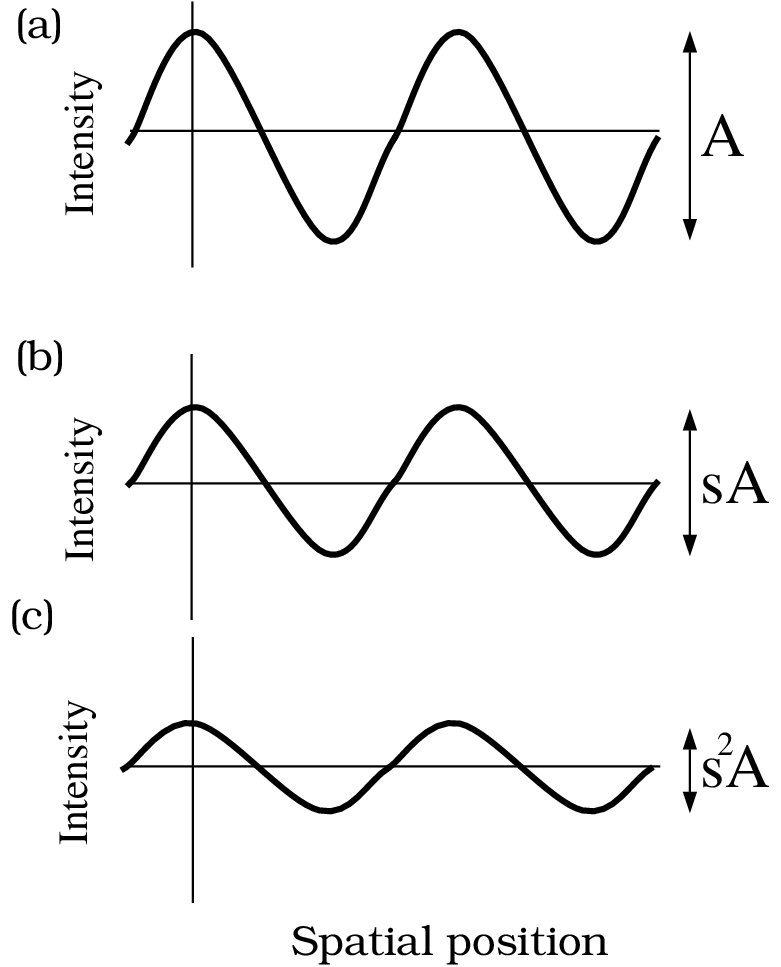
\includegraphics[width=0.5\textwidth,height=\textheight]{wp-content/uploads/2012/02/doublepass.png}

}

\caption{\label{fig-doublepass}Sinusoids and Double Passage (a) The
amplitude, A, of an input cosinusoid stimulus is scaled by a factor, s,
after passing through even-symmetric shift-invariant symmetric optics as
shown in part (b). (c) Passage through the optics a second time scales
the amplitude again, resulting in a signal with amplitude s\^{}2 A.}

\end{figure}%

To understand how to correct for double passage, consider a hypothetical
alternative experiment Campbell and Gubisch might have done
(Figure~\ref{fig-doublepass}). Suppose Campbell and Gubisch had used
input stimuli equal to cosinusoids at various spatial frequencies,
\(f\). Because the optics are shift-invariant and there is no
frequency-dependent phase shift, the retinal image of a cosinusoid at
frequency \(f\) is a cosinusoid scaled by a factor \(s_f\). The retinal
image passes back through the optics and is scaled again, so that the
measurement would be a cosinusoid scaled by the factor \(s_f^2\). Hence,
had Campbell and Gubisch used a cosinusoidal input stimulus, we could
deduce the retinal image from the measured image easily: The retinal
image would be a cosinusoid with an amplitude equal to the square root
of the amplitude of the measurement.

Campbell and Gubisch used a single line, not a set of cosinusoidal
stimuli. But, we can still apply the basic idea of the hypothetical
experiment to their measurements. Their input stimulus, defined over
\(N\) locations, is

\begin{equation}\phantomsection\label{eq-single-line-stimulus}{
\mathbf{p}_{i} = \left\{
\begin{array}{ll}
1 & \text{if } i=0 \\
0 & \text{if } 1 \leq i < N
\end{array}
\right.
}\end{equation}

As I describe in the appendix, we can express the stimulus as the
weighted sum of harmonic functions by using the \emph{discrete Fourier
series}. The representation of a single line is equal to the sum of
cosinusoidal functions

\begin{equation}\phantomsection\label{eq-fourier-single-line}{
\mathbf{p}_{i} = 0.5 + \sum_{f=1}^{N-1} \cos\left( 2 \pi f \frac{i}{N} \right)
}\end{equation}

Because the system is shift-invariant, the retinal image of each
cosinusoid was a scaled cosinusoid, say with scale factor \(s_f\). The
retinal image was scaled again during the second pass through the
optics, to form the cosinusoidal term they measured.\footnote{Be
  bothered by the fact that the discrete Fourier series approximation is
  an infinite set of pulses, rather than a single line. To understand
  why, consult the Appendix.}

Using the discrete Fourier series, we also can express the measurement
as the sum of cosinusoidal functions,

\begin{equation}\phantomsection\label{eq-measurement}{
\text{Measurement} = 0.5 + \sum_{f=1}^{N-1} (s_f)^2 \cos\left( 2 \pi f \frac{i}{N} \right)
}\end{equation}

We know the values of \(s_f^2\), since this was Campbell and Gubisch's
measurement. The image of the line at the retina, then, must have been

\begin{equation}\phantomsection\label{eq-retinal-image}{
\mathbf{l}_{i} = 0.5 + \sum_{f=1}^{N-1} s_f \cos\left( 2 \pi f \frac{i}{N} \right)
}\end{equation}

The values \(\mathbf{l}_{i}\) define the linespread function of the
eye's optics. We can correct for the double passage and estimate the
linespread because the system is linear and shift-invariant.

As you read further about experimental and computational methods in
vision science, remember that there is nothing inherently important
about sinusoids as visual stimuli; we must not confuse the stimulus with
the system or with the theory we use to analyze the system. When the
system is a shift-invariant linear system, sinusoids can be helpful in
simplifying our calculations and reasoning, as we have just seen. The
sinusoidal stimuli are important only insofar as they help us to measure
or clarify the properties of the system. And if the system is not
shift-invariant, the sinusoids may not be important at all.

\subsection{The Linespread Function}\label{sec-linespread}

Figure~\ref{fig-linespread} contains Campbell and Gubisch's estimates of
the linespread functions of the eye. Notice that as the pupil size
increases, the width of the linespread function increases which
indicates that the focus is worse for larger pupil sizes. As the pupil
size increases, light reaches the retina through larger and larger
sections of the lens. As the area of the lens affecting the passage of
light increases, the amount of blurring increases.

\begin{figure}

\centering{

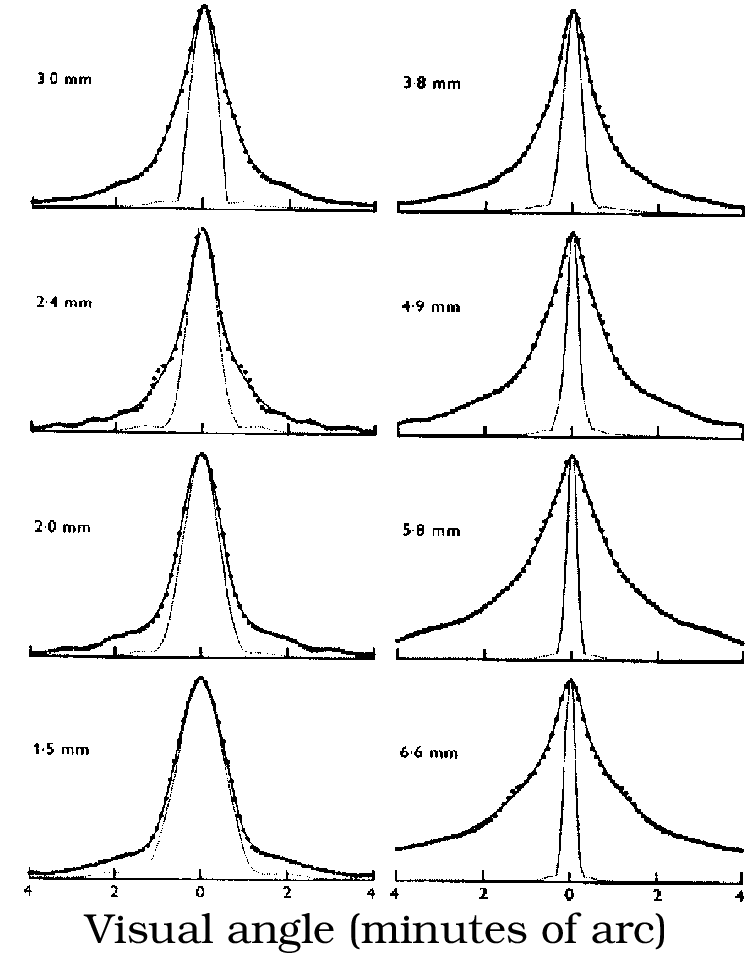
\includegraphics[width=0.6\textwidth,height=\textheight]{wp-content/uploads/2012/02/cg.linespread.png}

}

\caption{\label{fig-linespread}The linespread function of the human eye:
The solid line in each panel is a measurement of the linespread. The
dotted lines are the diffraction-limited linespread for a pupil of that
diameter. (Diffraction is explained later in the text). The different
panels show measurements for a variety of pupil diameters (From Campbell
and Gubisch (1966)).}

\end{figure}%

The measured linespread functions, \(\mathbf{l}_{i}\), along with our
belief that we are studying a shift-invariant linear system, permit us
to predict the retinal image for any one-dimensional input image. To
calculate these predictions, it is convenient to have a function that
describes the linespread of the human eye. G. Westheimer (Westheimer
(1986)) suggested the following formula to describe the measured
linespread function of the human eye, when in good focus, and when the
pupil diameter is near 3mm\footnote{Westheimer's linespread function is
  for an average observer under one set of viewing conditions. As the
  pupil changes size and as observer's age, the linespread function can
  vary. Consult IJspeert et al. (1993) and Williams et al. (1994) for
  alternatives to Westheimer's formula.}.

\begin{equation}\phantomsection\label{eq-westheimer-linespread}{
\mathbf{l}_{i} = 0.47 e^{ - 3.3 i ^ {2} } + 0.53 e ^ { -0.93 | i | }
}\end{equation}

\begin{figure}

\centering{

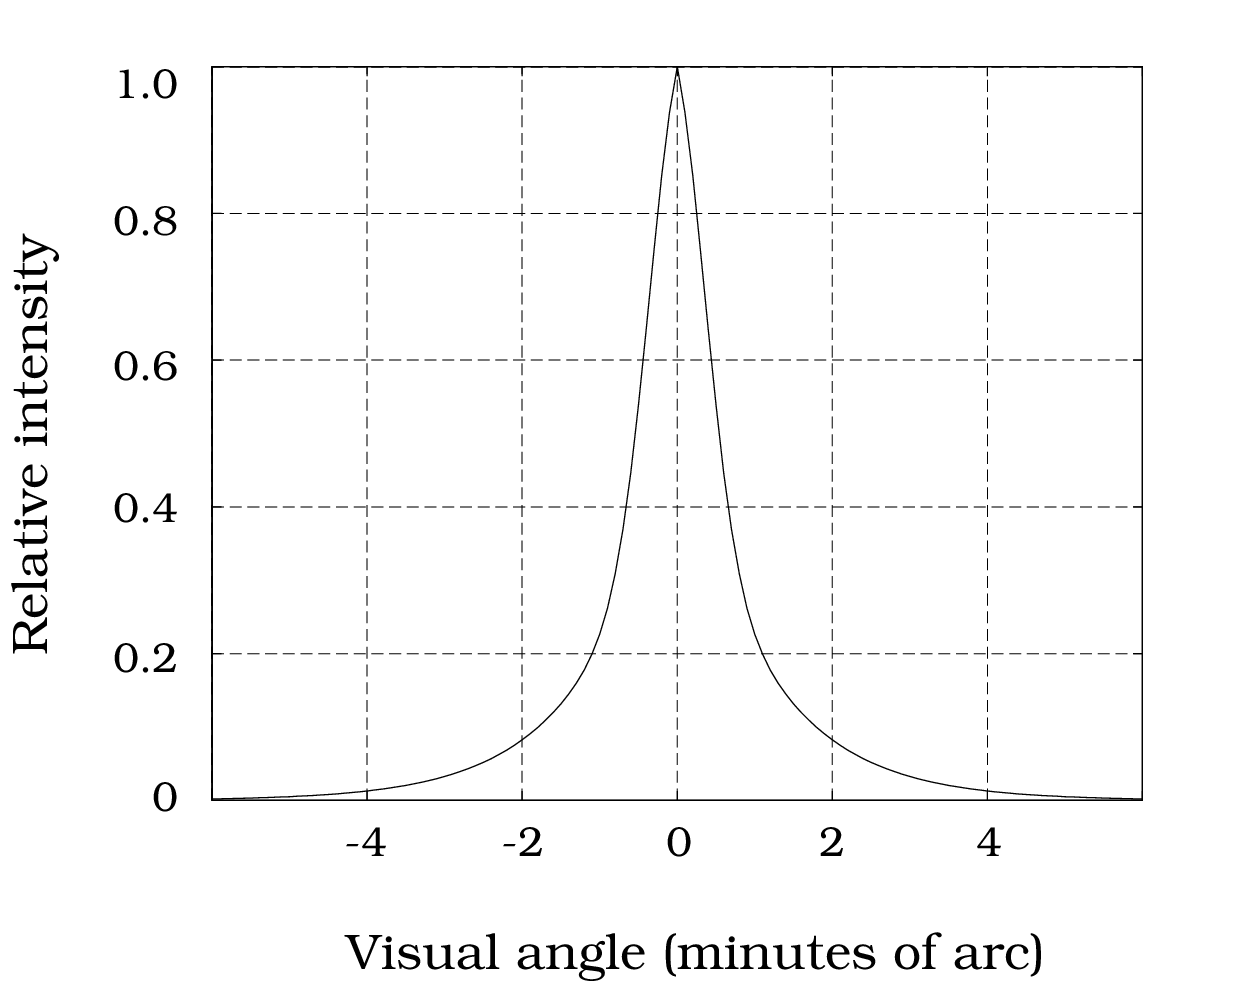
\includegraphics[width=0.6\textwidth,height=\textheight]{wp-content/uploads/2012/02/westheimer.ls_.png}

}

\caption{\label{fig-westheimer-linespread}Westheimer's Linespread
Function. Analytic approximation of the human linespread function for an
eye with a 3.0mm diameter pupil (Westheimer and Tanzman (1956)).}

\end{figure}%

The linespread function is given by:

\begin{equation}\phantomsection\label{eq-westheimer-linespread-inline}{
\mathbf{l}_{i} = 0.47 e^{ - 3.3 i ^ {2} } + 0.53 e ^ { -0.93 | i | }
}\end{equation}

where the variable \(i\) refers to position on the retina specified in
terms of minutes of visual angle. A graph of this linespread function is
shown in Equation~\ref{eq-westheimer-linespread}.

\subsection{The Modulation Transfer
Function}\label{the-modulation-transfer-function}

\begin{figure}

\centering{

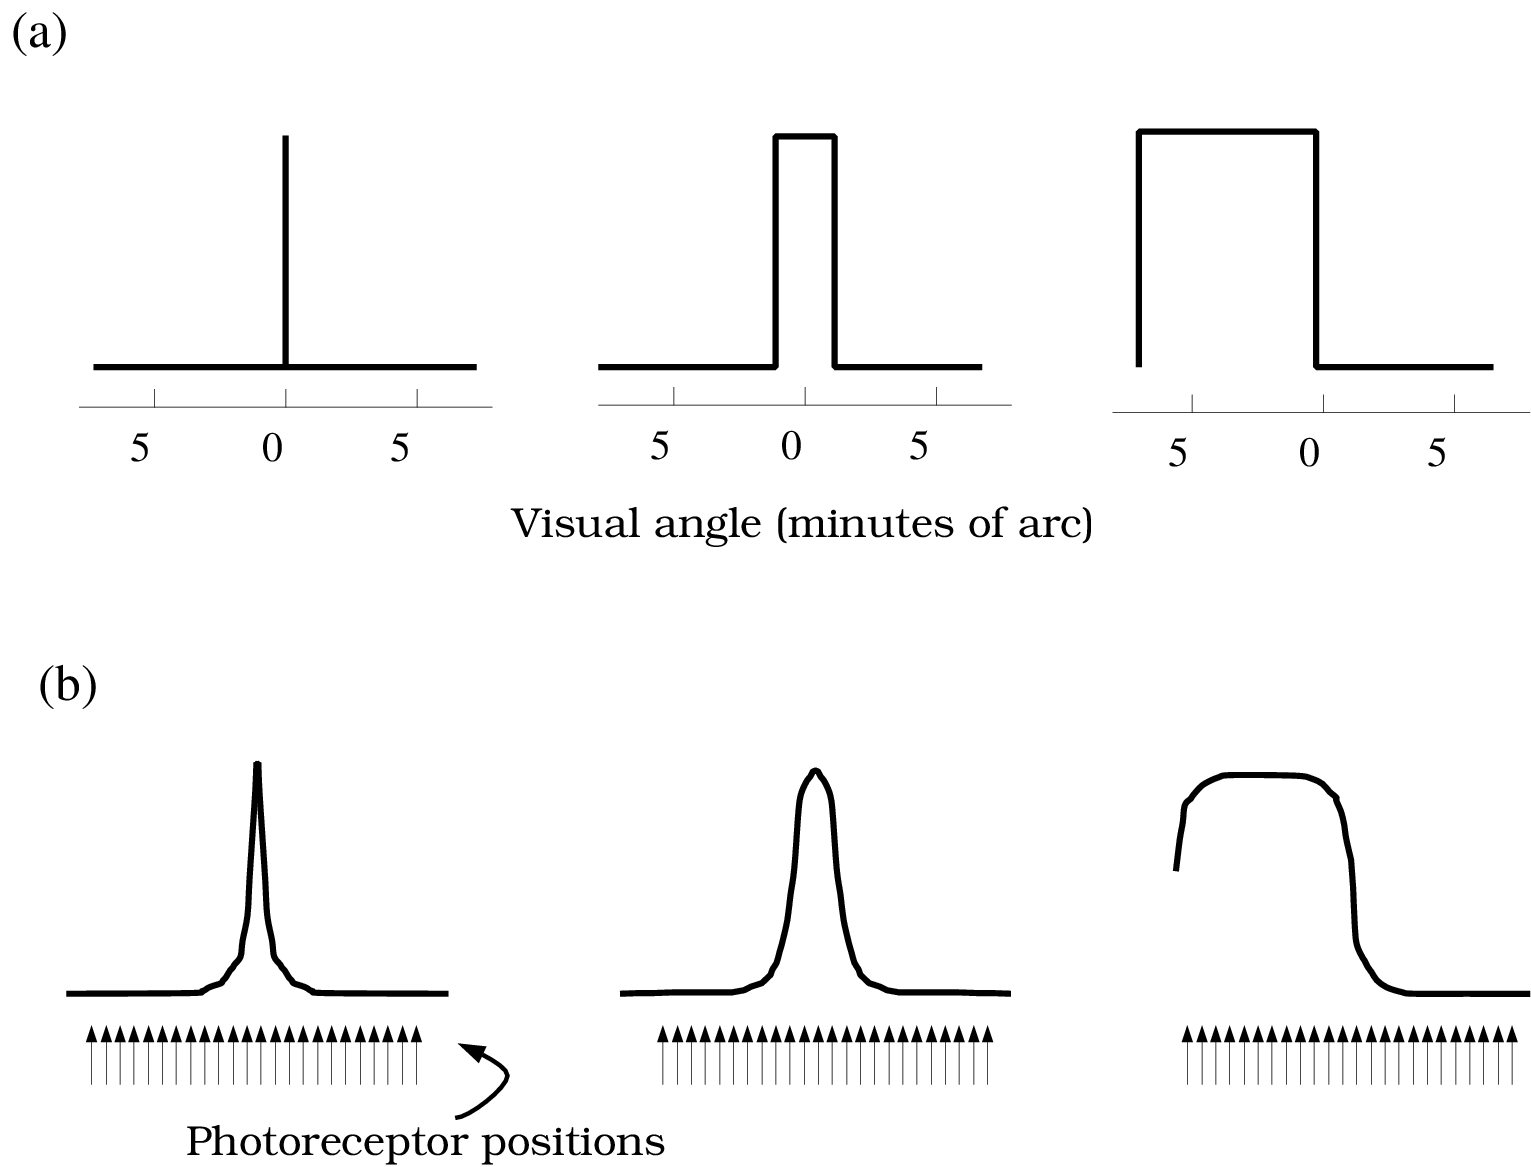
\includegraphics[width=0.7\textwidth,height=\textheight]{wp-content/uploads/2012/02/blurring.png}

}

\caption{\label{fig-retinal-blurring}Retinal Images. Examples of the
effect of optical blurring. (a) Images of a line, edge and a bar
pattern. (b) The estimated retinal image of the images after blurring by
Westheimer's linespread function. The spacing of the photoreceptors in
the retina is shown by the stylized arrows.}

\end{figure}%

In correcting for double passage, we thought about the measurements in
two separate ways. Since our main objective was to derive the linespread
function, a function of spatial position, we spent most of our time
thinking of the measurements in terms of light intensity as a function
of spatial position. When we corrected for double passage through the
optics, however, we also considered a hypothetical experiment in which
the stimuli were harmonic functions (cosinusoids). To perform this
calculation, we found that it was easier to correct for double passage
by thinking of the stimuli as the sum of harmonic functions, rather than
as a function of spatial position.

These two ways of looking at the system, in terms of spatial functions
or sums of harmonic functions, are equivalent to one another. To see
this, notice that we can use the linespread function to derive the
retinal image to any input image. Hence, we can use the linespread to
compute the scale factors of the harmonic functions. Conversely, we
already saw that by measuring how the system responds to the harmonic
functions, we can derive the linespread function. It is convenient to be
able to reason about system performance in both ways.

\begin{figure}

\centering{

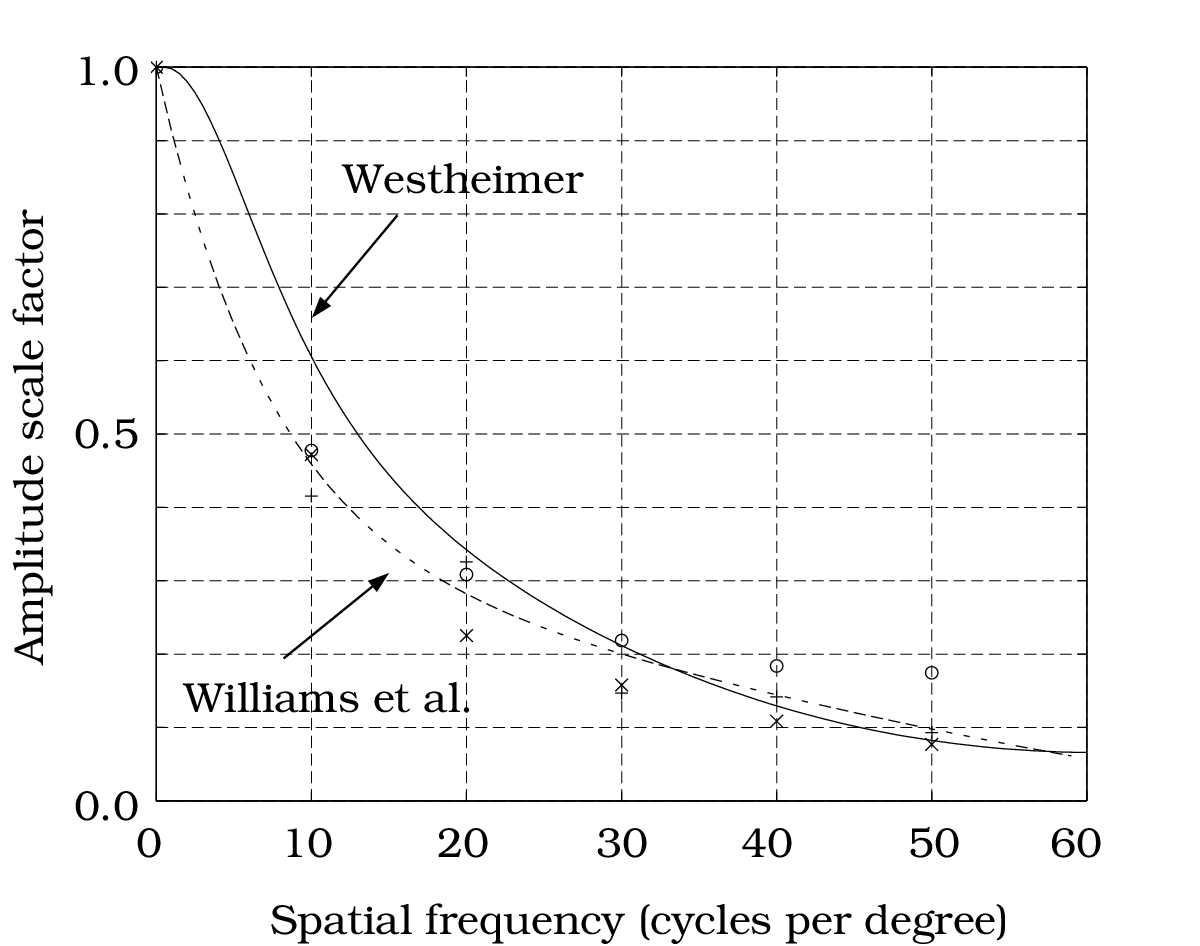
\includegraphics[width=0.7\textwidth,height=\textheight]{wp-content/uploads/2012/02/otfDataTheory.png}

}

\caption{\label{fig-modulation-transfer}Modulation transfer function
measurements of the optical quality of the lens made using visual
interferometry (Williams et al. (1994); described in
Chapter~\ref{sec-photoreceptor-mosaic}). The data are compared with the
predictions from the linespread suggested by Westheimer (1986) and a
curve fit through the data by Williams et al. (1994).}

\end{figure}%

The \emph{optical transfer function} defines the system's complete
response to harmonic functions. The optical transfer function is a
complex-valued function of spatial frequency. The complex values code
both the scale factor and the phase shift the system induces in each
harmonic function.

When the linespread function of the eye is an even-symmetric function,
there is no phase shift of the harmonic functions. In this case, we can
describe the system completely using a real valued function, the
\emph{modulation transfer function}. This function defines the scale
factors applied to each spatial frequency. The data points in
Figure~\ref{fig-modulation-transfer} show measurements of the modulation
transfer function of the human eye. These data points were measured
using a method called \emph{visual interferometry} that is described in
Chapter~\ref{sec-photoreceptor-mosaic}. Along with the data points in
Figure~\ref{fig-modulation-transfer}, I have plotted the predicted
modulation transfer function using Westheimer's linespread function and
a curve fit to the data by Williams et al. (1994). The curve derived by
Westheimer (1986) using completely different data sets differs from the
measurements by Williams et al. (1994) by no more than about twenty
percent. This should tell you something about the relative precision of
these descriptions of the optical quality of the lens.

The linespread function and the modulation transfer function offer us
two different ways to think about the optical quality of the lines. The
linespread function in Figure~\ref{fig-modulation-transfer}, describes
defocus as the spread of light from a fine slit across the
photoreceptors: the light is spread across three to five photoreceptors.
The modulation transfer function in Figure~\ref{fig-modulation-transfer}
describes defocus as an amplitude reduction of harmonic stimuli: beyond
12 cycles per degree the amplitude is reduced by more than a factor of
two.

\section{Lenses, Diffraction and
Aberrations}\label{sec-lensesdiffractionandaberrations}

\subsection{Lenses and Accommodation}\label{sec-lensesaccommodation}

What prevents the optics of our eye from focusing the image perfectly?
To answer this question we should consider why a lens is useful in
bringing objects to focus at all.

\begin{figure}

\centering{

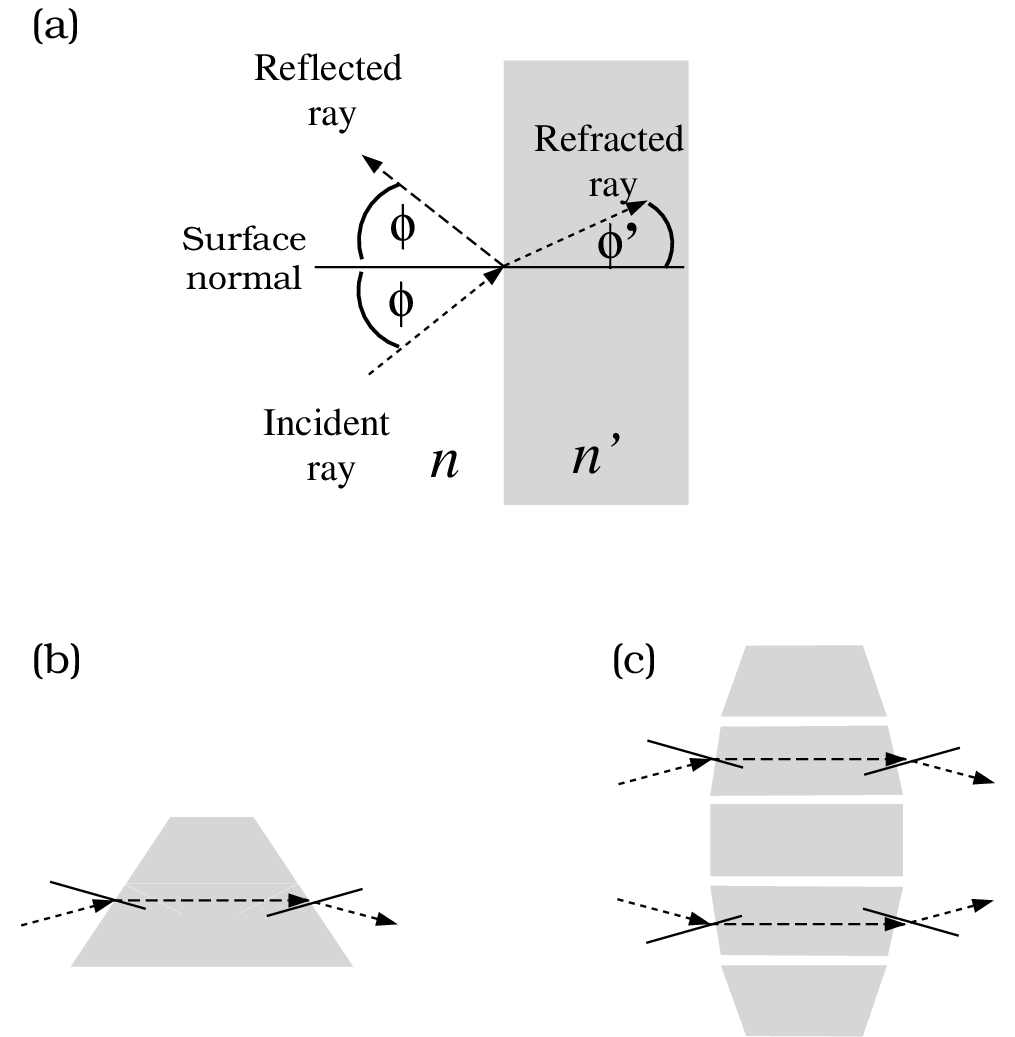
\includegraphics[width=0.4\textwidth,height=\textheight]{wp-content/uploads/2012/02/snell2.png}

}

\caption{\label{fig-snell-law}Snell's law. The solid lines indicate
surface normals and the dashed lines indicate the light ray. (a) When a
light ray passes from one medium to another, the ray can be refracted so
that the angle of incidence (phi) does not equal the angle of refraction
(phi `). Instead, the angle of refraction depends on the refractive
indices of the new media (n and n') a relationship called Snell's law
that is defined in Equation~\ref{eq-snell} (after Jenkins and White
(1937) figures 1H page 15 and 2H page 30.) (b) A prism causes two
refractions of the light ray and can reverse the ray's direction from
upward to downward. (c) A lens combines the effect of many prisms in
order to converge the rays diverging from a point source. (After Jenkins
and White (1937) figure 1F, page 12.)}

\end{figure}%

As a ray of light is reflected from an object, it will travel along
along a straight line until it reaches a new material boundary. At that
point, the ray may be either absorbed by the new medium, reflected, or
refracted. The latter two possibilities are illustrated in part (a) of
Figure~\ref{fig-snell-law}. We call the angle between the incident ray
of light and the perpendicular to the surface the \emph{angle of
incidence}. The angle between the reflected ray and the perpendicular to
the surface is called the \emph{angle of reflection}, and it equals the
angle of incidence. Of course, reflected light is not useful for image
formation at all.

The useful rays for imaging must pass from the first medium into the
second. As they pass from between the two media, the ray's direction is
\emph{refracted}. The angle between the refracted ray and the
perpendicular to the surface is called the \emph{angle of refraction}.

The relationship between the angle of incidence and the angle of
refraction was first discovered by a Dutch astronomer and mathematician,
Willebrord Snell in 1621. He observed that when \(\phi\) is the angle of
incidence, and \(\phi'\) is the angle of refraction, then

\begin{equation}\phantomsection\label{eq-snell}{
\frac{ \sin \phi } { \sin \phi' } = \frac{\nu'}{\nu}
}\end{equation}

The terms \(\nu'\) and \(\nu\) in Equation~\ref{eq-snell} are the
\emph{refractive indices} of the two media. The refractive index of an
optical medium is the ratio of the speed of light in a vacuum to the
speed of light in the optical medium. The refractive index of glass is
\(1.520\), for water the refractive index is \(1.333\) and for air it is
nearly \(1.000\). The refractive index of the human cornea is \(1.376\),
which is quite similar to water, the main content of our eyes.

Now, consider the consequence of applying Snell's law twice in a row as
light passes into and then out of a prism, as illustrated in part (b) of
Figure~\ref{fig-snell-law}. We can draw the path of the ray as it enters
the prism using Snell's law. The symmetry of the prism and the
reversibility of the light path makes it easy to draw the exit path.
Passage through the prism bends the ray's path downward. The prism
causes the light to deviate significantly from a straight path; the
amount of the deviation depends upon the angle of incidence and the
angle between the two sides of the prism.

We can build a lens by smoothly combining many infintesimally small
prisms to form a convex lens, as illustrated in part (c) of
Figure~\ref{fig-snell-law}. In constructing such a lens, any deviations
from the smooth shape, or imperfections in the material used to build
the lens, will cause the individual rays to be brought to focus at
slightly different points in the image plane. These small deviations of
shape or materials are a source of the imperfections in the image.

Objects at different depths are focused at different distances behind
the lens. The \emph{thin lens equation} relates the distance between the
source and the lens with the distance between the image and the lens.
The thin lens equation relating these two distances depends on the
\emph{focal length} of the lens. Call the distance from the center of
the lens to the source \(d_s\), the distance to the image \(d_i\), and
the focal length of the lens, \(f\). Then the thin lens equation is

\begin{equation}\phantomsection\label{eq-thin-lens}{
\frac{1}{d_s} + \frac{1}{d_i} = \frac{1}{f}
}\end{equation}

From this equation, notice that we can measure the focal length of a
convex thin lens by using it to image a very distant object. In that
case, the term \(\frac{1}{d_s}\) is zero so that the image distance is
equal to the focal length. When I first moved to California, I spent a
lot of time measuring the focal length of the lenses in my laboratory by
going outside and imaging the sun on a piece of paper behind the lens;
the sun was a convenient source at optical infinity. It had been a less
reliable source for me in my previous home.

\begin{figure}

\centering{

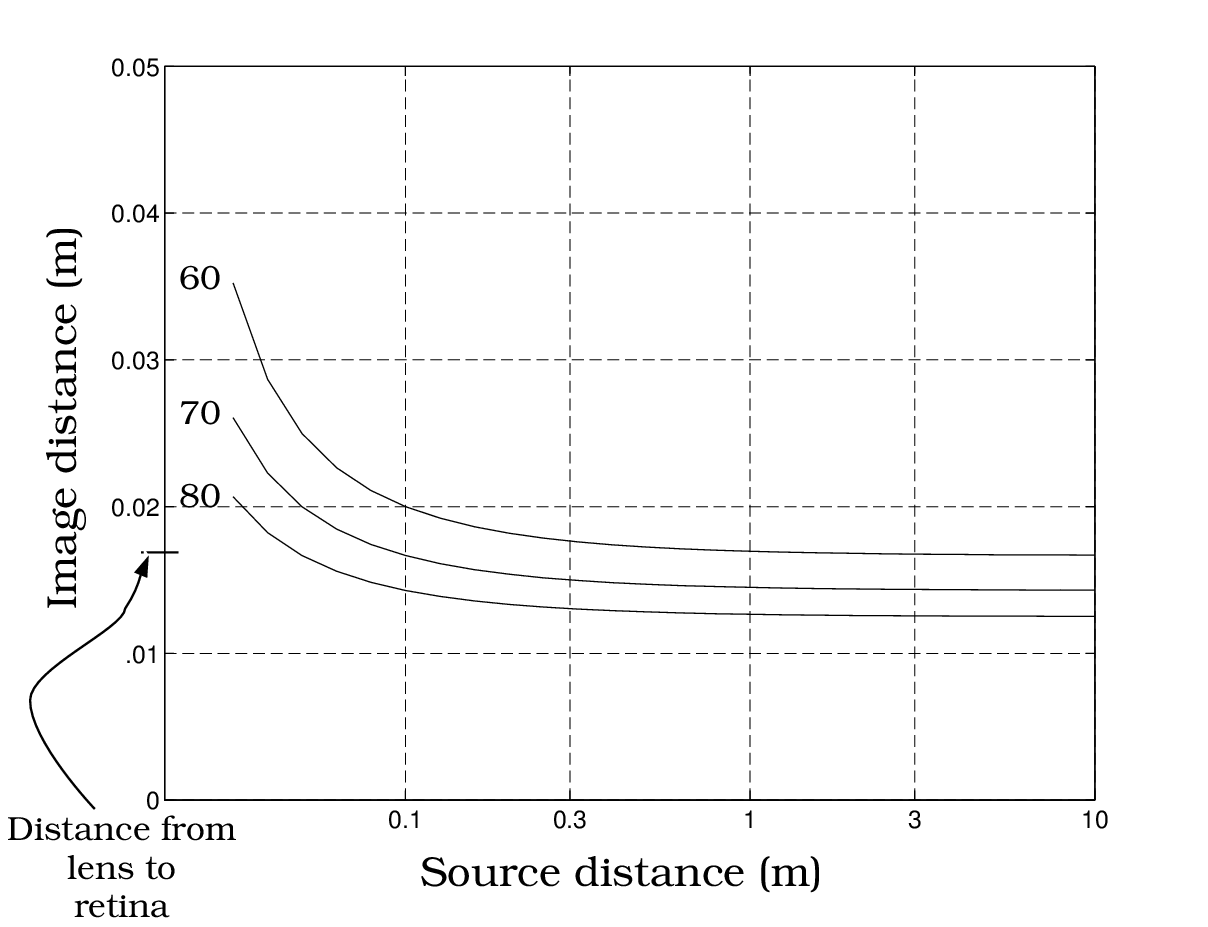
\includegraphics[width=0.6\textwidth,height=\textheight]{wp-content/uploads/2012/02/accommodation.png}

}

\caption{\label{fig-accommodation}Depth of Field in the Human Eye. Image
distance is shown as a function of source distance. The bar on the
vertical axis shows the distance of the retina from the lens center. A
lens power of 60 diopters brings distant objects into focus, but not
nearby objects; to bring nearby objects into focus the power of the lens
must increase. The depth of field, namely the distance over which
objects will continue to be in reasonable focus, can be estimated from
the slope of the curve.}

\end{figure}%

The optical \emph{power} of a lens is a measure of how strongly the lens
bends the incoming rays. Since a short focal length lens bends the
incident ray more than a long focal length lens, the optical power is
inversely related to focal length. The optical power is defined as the
reciprocal of the focal length measured in meters and is specified in
units of \emph{diopters}. When we view far away objects, the distance
from the middle of the cornea and the flexible lens to the retina is
\(0.017\,\mathrm{m}\). Hence, the optical power of the human eye is
\(\frac{1}{0.017} = 58.8\), or roughly \(60\) diopters.

From the optical power of the eye (\(1/f\)) and the thin lens equation,
we can calculate the image distance of a source at distance. For
example, the top curve in Figure~\ref{fig-accommodation} shows the
relationship between image distance \(d_i\) and source distance \(d_s\)
for a 60 diopter lens. Sources beyond 1.0m are imaged at essentially the
same distance behind the optics. Sources closer than 1.0m are imaged at
a longer distance, so that the retinal image is blurred.

To bring nearby sources into focus on the retina, muscles attached to
the lens change its shape and thus change the power of the lens. The
bottom two curves in Figure~\ref{fig-accommodation} illustrate that
sources closer than 1.0m can be focused onto the retina by increasing
the power of the lens. The process of adjusting the focal length of the
lens is called \emph{accommodation}. You can see the effect of
accommodation by first focusing on your finger placed near your noise
and noticing that objects in the distance appear blurred. Then, while
leaving your finger in place, focus on the distant objects. You will
notice that your finger now appears blurred.

\subsection{Pinhole Optics and
Diffraction}\label{sec-PinholeOpticsandDiffraction}

The only way to remove lens imperfections completely is to remove the
lens. It is possible to focus images without any lens at all by using
\emph{pinhole} optics, as illustrated in
Figure~\ref{fig-pinhole-optics}.

\begin{figure}

\centering{

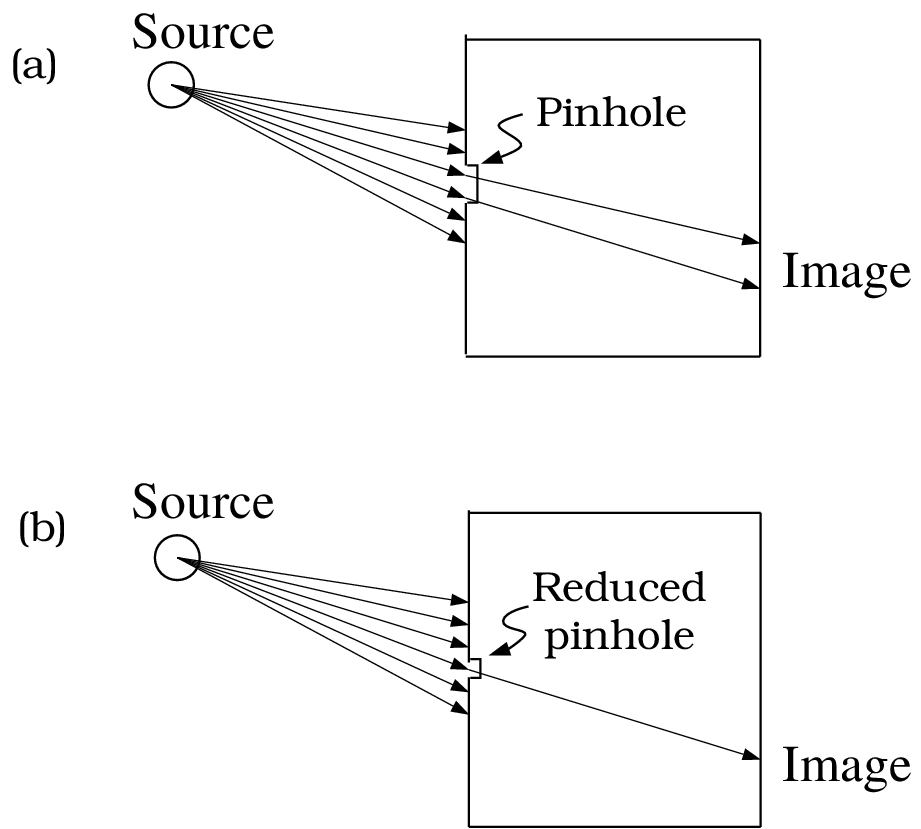
\includegraphics[width=0.6\textwidth,height=\textheight]{wp-content/uploads/2012/02/pinhole.png}

}

\caption{\label{fig-pinhole-optics}Pinhole Optics. Using ray-tracing, we
see that only a small pencil of rays passes through a pinhole. (a) If we
widen the pinhole, light from the source spread across the image, making
it blurry. (b) If we narrow the pinhole, only a small amount of light is
let in. The image is sharp; the sharpness is limited by diffraction.}

\end{figure}%

A pinhole serves as a useful focusing element because only the rays
passing within a narrow angle are used to form the image. As the pinhole
is made smaller, the angular deviation is reduced. Reducing the size of
the pinhole serves to reduce the amount of blur due to the deviation
amongst the rays. Another advantage of using pinhole optics is that no
matter how distant the source point is from the pinhole, the source is
rendered in sharp focus. Since the focusing is due to selecting out a
thin pencil of rays, the distance of the point from the pinhole is
irrelevant and accommodation is unnecessary.

But the pinhole design has two disadvantages. First, as the pinhole
aperture is reduced, less and less of the light emitted from the source
is used to form the image. The reduction of signal has many
disadvantages for sensitivity and acuity.

A second fundamental limit to the pinhole design is a physical
phenomenon. When light passes through a small aperture, or near the edge
of an aperture, the rays do not travel in a single straight line.
Instead, the light from a single ray is scattered into many directions
and produces a blurry image. The dispersion of light rays that pass by
an edge or narrow aperture is called \emph{diffraction}. Diffraction
scatters the rays coming from a small source across the retinal image
and therefore serves to defocus the image. The effect of diffraction
when we take an image using pinhole optics is shown in
Figure~\ref{fig-diffraction-pinhole}.

\begin{figure}

\centering{

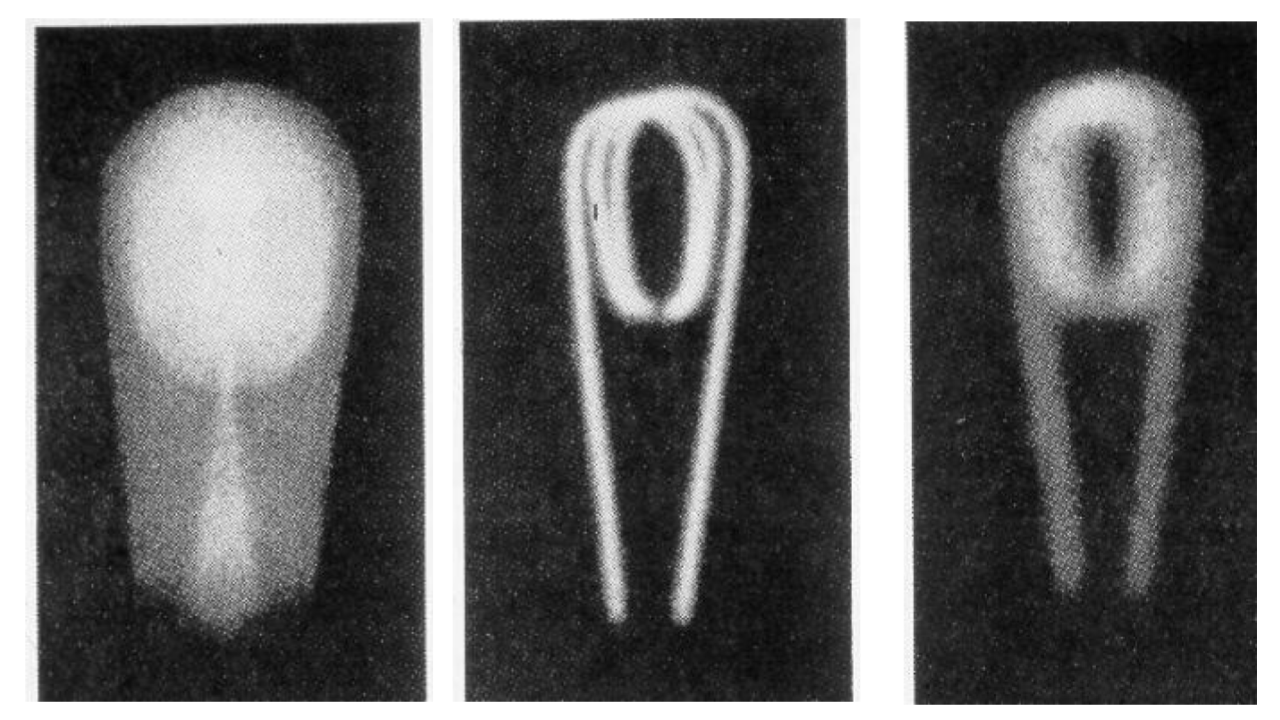
\includegraphics[width=0.5\textwidth,height=\textheight]{wp-content/uploads/2012/02/filamentnew.png}

}

\caption{\label{fig-diffraction-pinhole}Diffraction limits the quality
of pinhole optics. The three images of a bulb filament were imaged using
pinholes with decreasing size. (a) When the pinhole is relatively large,
the image rays are not properly converged and the image is blurred. (b)
Reducing the pinhole improves the focus. (c) Reducing the pinhole
further worsens the focus due to diffraction.}

\end{figure}%

Diffraction can be explained in two different ways. First, diffraction
can be explained by thinking of light as a wave phenomenon. A wave
exiting from a small aperture expands in all directions; a pair of
coherent waves from adjacent apertures create an interference pattern.
Second diffraction can be understood in terms of quantum mechanics;
indeed, the explanation of diffraction is one of the important
achievements of quantum mechanics. Quantum mechanics supposes that there
are limits to how well we may know both the position and direction of
travel of a photon of light. The more we know about a photon's position,
the less we can know about its direction. If we know that a photon has
passed through a small aperture, then we know something about the
photon's position and we must pay a price in terms of our uncertainty
concerning its direction of travel. As the aperture becomes smaller, our
certainty concerning the position of the photon becomes greater; this
uncertainty takes the form of the scattering of the direction of travel
of the photons as they pass through the aperture. For very small
apertures, for which our position certainty is high, the photon's
direction of travel is very broad producing a very blurry image.

There is a close relationship between the uncertainty in the direction
of travel and the shape of the aperture (Figure~\ref{fig-diffraction}).
In all cases, however, when the aperture is relatively large, our
knowledge of the spatial position of the photons is insignificant and
diffraction does not contribute to defocus. As the pupil size decreases,
and we know more about the position of the photons, the diffraction
pattern becomes broader and spoils the focus.

\begin{figure}

\centering{

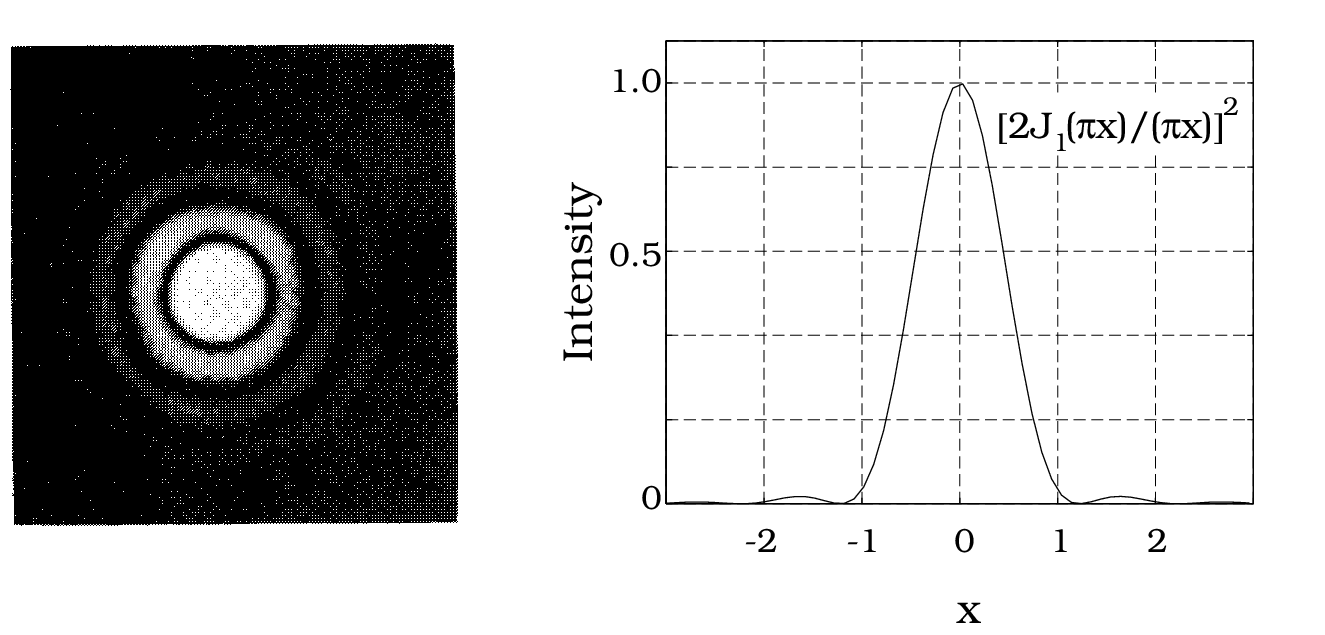
\includegraphics[width=0.5\textwidth,height=\textheight]{wp-content/uploads/2012/02/diffraction.png}

}

\caption{\label{fig-diffraction}Diffraction: Diffraction pattern caused
by a circular aperture. (a) The image of a diffraction pattern measured
through a circular aperture. (b) A graph of the cross-sectional
intensity of the diffraction pattern. (After Goodman (1968)).}

\end{figure}%

In the human eye diffraction occurs because light must pass through the
circular aperture defined by the pupil. When the ambient light intensity
is high, the pupil may become as small as \(2\,\mathrm{mm}\) in
diameter. For a pupil opening this small, the optical blurring in the
human eye is due only to the small region of the cornea and lens near
the center of our visual field. With this small an opening of the pupil,
the quality of the cornea and lens is rather good and the main source of
image blur is diffraction. At low light intensities, the pupil diameter
is as large as \(8\,\mathrm{mm}\). When the pupil is open quite wide,
the distortion due to cornea and lens imperfections is large compared to
the defocus due to diffraction.

One way to evaluate the quality of the optics is to compare the blurring
of the eye to the blurring from diffraction alone. The dashed lines in
Figure~\ref{fig-imgfor-cg-data} plot the blurring expected from
diffraction for different pupil widths. Notice that when the pupil is
2.4\textasciitilde mm, the observed linespread is about equal to the
amount expected by diffraction alone; the lens causes no further
distortion. As the pupil opens, the observed linespread is worse than
the blurring expected by diffraction alone. For these pupil sizes the
defocus is due mainly to imperfections in the optics\footnote{Helmholtz
  calculated that this was so long before any precise measurements of
  the optical quality of the eye were possible. He wrote, ``The limit of
  the visual capacity of the eye as imposed by diffraction, as far as it
  can be calculated, is attained by the visual acuity of the normal eye
  with a pupil of the size corresponding to a good illumination.'' From
  Helmholtz, Phys. Optics I, page 442 (Helmholtz (1866/1911), p.~442).}.

\subsection{The Pointspread Function and
Astigmatism}\label{sec-ThePointspreadFunctionandAstigmatism}

\begin{figure}

\centering{

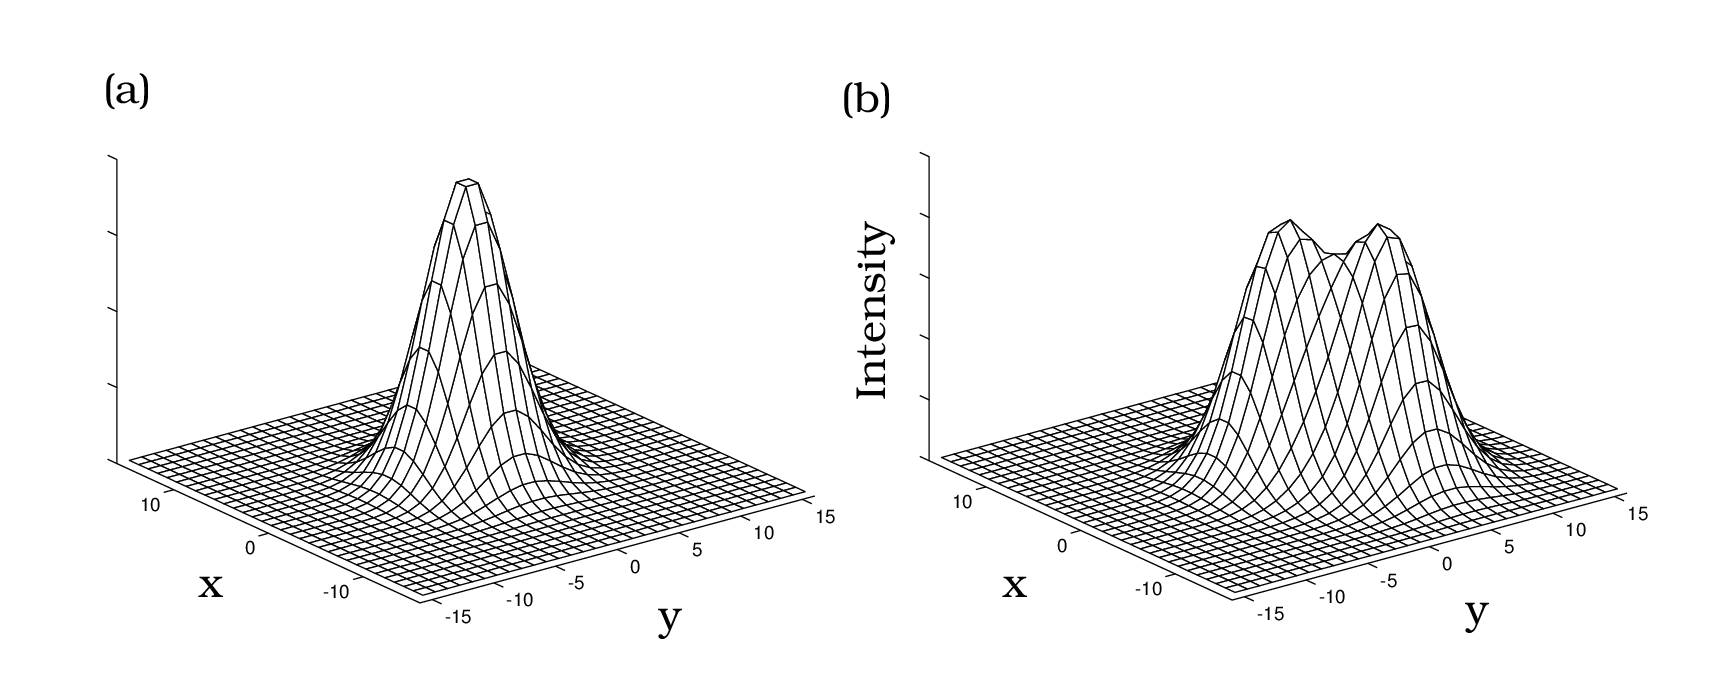
\includegraphics[width=0.7\textwidth,height=\textheight]{wp-content/uploads/2012/02/pointspread1.png}

}

\caption{\label{fig-pointspread}Pointspread Function: A pointspread
function. (a) and the sum of two pointspreads (b). The pointspread
function is the image created by a source consisting of a small point of
light. When the optics shift-invariant, the image to any stimulus can be
predicted from the pointspread function.}

\end{figure}%

Most images, of course, are not composed of weighted sums of lines. The
set of images that can be formed from sums of lines oriented in the same
direction are all one-dimensional patterns. To create more complex
images, we must either use lines with different orientations or use a
different fundamental stimulus: the point.

Any two-dimensional image can be described as the sum of a set of
points. If the system we are studying is linear and shift-invariant, we
can use the response to a point and the principle of superposition to
predict the response of a system to any two-dimensional image. The
measured response to a point input is called the \emph{pointspread}\}*
function. A pointspread function and the superposition of two nearby
pointspreads are illustrated in Figure~\ref{fig-pointspread}.

Since lines can be formed by adding together many different points, we
can compute the system's linespread function from the pointspread. In
general, we cannot deduce the pointspread function from the linespread
because there is no way to add a set of lines, all oriented in the same
direction, to form a point. If it is know that a pointspread function is
circularly symmetric, however, a unique pointspread function can be
deduced from the linespread function. The calculation is described in
the beginning of Goodman (1968) and in Yellott et al. (1984).

\begin{figure}

\centering{

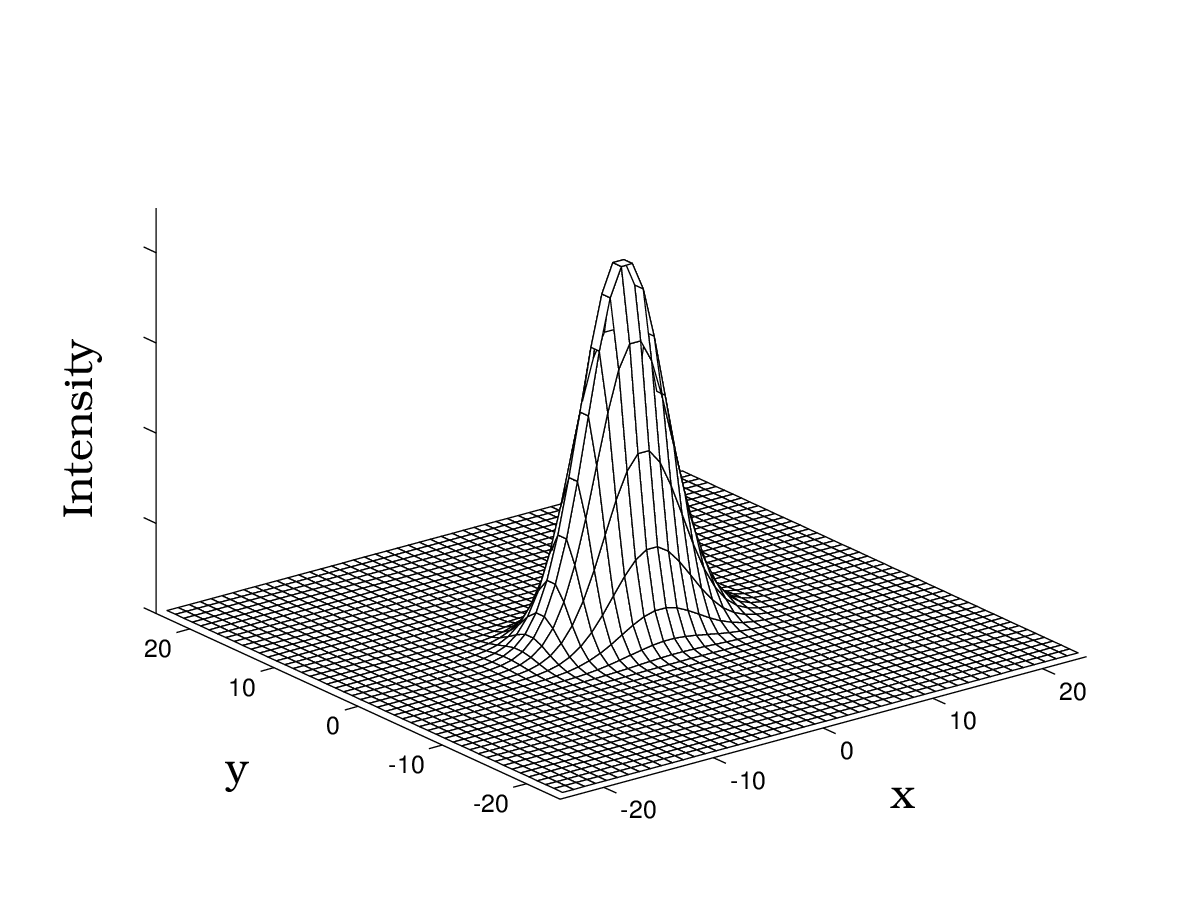
\includegraphics[width=0.7\textwidth,height=\textheight]{wp-content/uploads/2012/02/astigmatism.png}

}

\caption{\label{fig-astigmatism}Astigmatism: Astigmatism implies an
asymmetric pointspread function. The pointspread shown here is narrow in
one direction and wide in another. The spatial resolution of an
astigmatic system is better in the narrow direction than the wide
direction.}

\end{figure}%

When the pointspread functions is not circularly symmetric, measurements
of the linespread function will vary with the orientation of the test
line (Figure~\ref{fig-astigmatism}). It may be possible to adjust the
accommodation of this type of system so that any single orientation is
in good focus, but it will be impossible to bring all orientations into
good focus at the same time. For the human eye, astigmatism can usually
be modeled by describing the defocus as being derived from the
contributions of two one-dimensional systems at right angles to one
another. The defocus in intermediate angles can be predicted from the
defocus of these two systems.

\subsection{Chromatic Aberration}\label{sec-ChromaticAberration}

The light incident at the eye is usually a mixture of different
wavelengths. When we measure the system response, there is no guarantee
that the linespread or pointspread function we measure with different
wavelengths will be the same. Indeed, for most biological eyes the
pointspread function is very different as we measure using different
wavelengths of light. When the pointspread function of different
wavelengths of light is quite different, then the lens is said to
exhibit \emph{chromatic aberration}.

\begin{figure}

\centering{

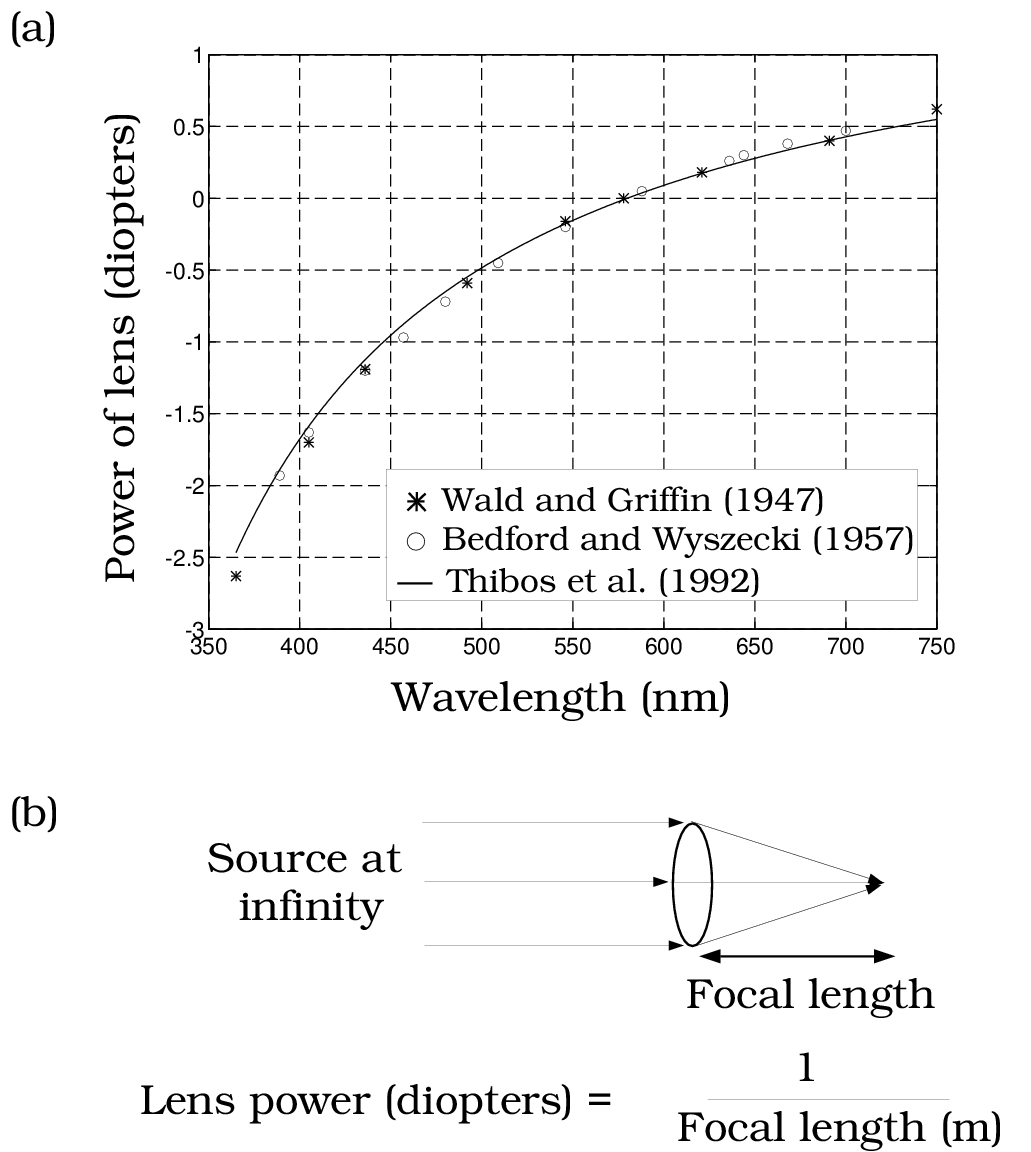
\includegraphics[width=0.6\textwidth,height=\textheight]{wp-content/uploads/2012/02/c.aberration.png}

}

\caption{\label{fig-chromatic-aberration}Chromatic Aberration: Chromatic
aberration of the human eye. (a) The data points are from Wald and
Griffin (1947), and Bedford and Wyszecki (1957). The smooth curve plots
the formula used by Thibos et al. (1992), D(λ) = p -- q / (λ -- c )
where λ is wavelength in micrometers, D(λ) is the defocus in diopters, p
=1.7312, q = 0.63346, and c = 0.21410. This formula implies an in-focus
wavelength of 578 nm. (b) The power of a thin lens is the reciprocal of
its focal length, which is the image distance from a source at infinity.
(After Marimont and Wandell (1992)).}

\end{figure}%

When the incident light is the mixture of many different wavelengths,
say white light, then we can see a chromatic fringe at edges. The fringe
occurs because the different wavelength components of the white light
are focused more or less sharply. Figure~\ref{fig-chromatic-aberration}
a plots one measure of the chromatic aberration. The smooth curve plots
the lens power, measured in units of \emph{em diopters} needed to bring
each wavelength into focus along with a 578nm light.

Figure~\ref{fig-chromatic-aberration} shows the optical power of a lens
necessary to correct for the chromatic aberration of the eye. When the
various wavelengths pass through the correcting lens, the optics will
have the same power as the eye's optics at 578nm. The two sets of
measurements agree well with one another and are similar to what would
be expected if the eye were simply a bowl of water. The smooth curve
through the data is a curve used by Thibos et al. (1992) to predict the
data.

An alternative method of representing the axial chromatic aberration of
the eye is to plot the modulation transfer function at different
wavelengths. The two surface plots in
Figure~\ref{fig-chromatic-aberration-otf} shows the modulation transfer
function at a series of wavelengths. The plots show the same data, but
seen from different points of view so that you can see around the hill.
The calculation in the figure is based on an eye with a pupil diameter
of 3.0mm, the same chromatic aberration as the human eye, and in perfect
focus except for diffraction at 580nm.

\begin{figure}

\centering{

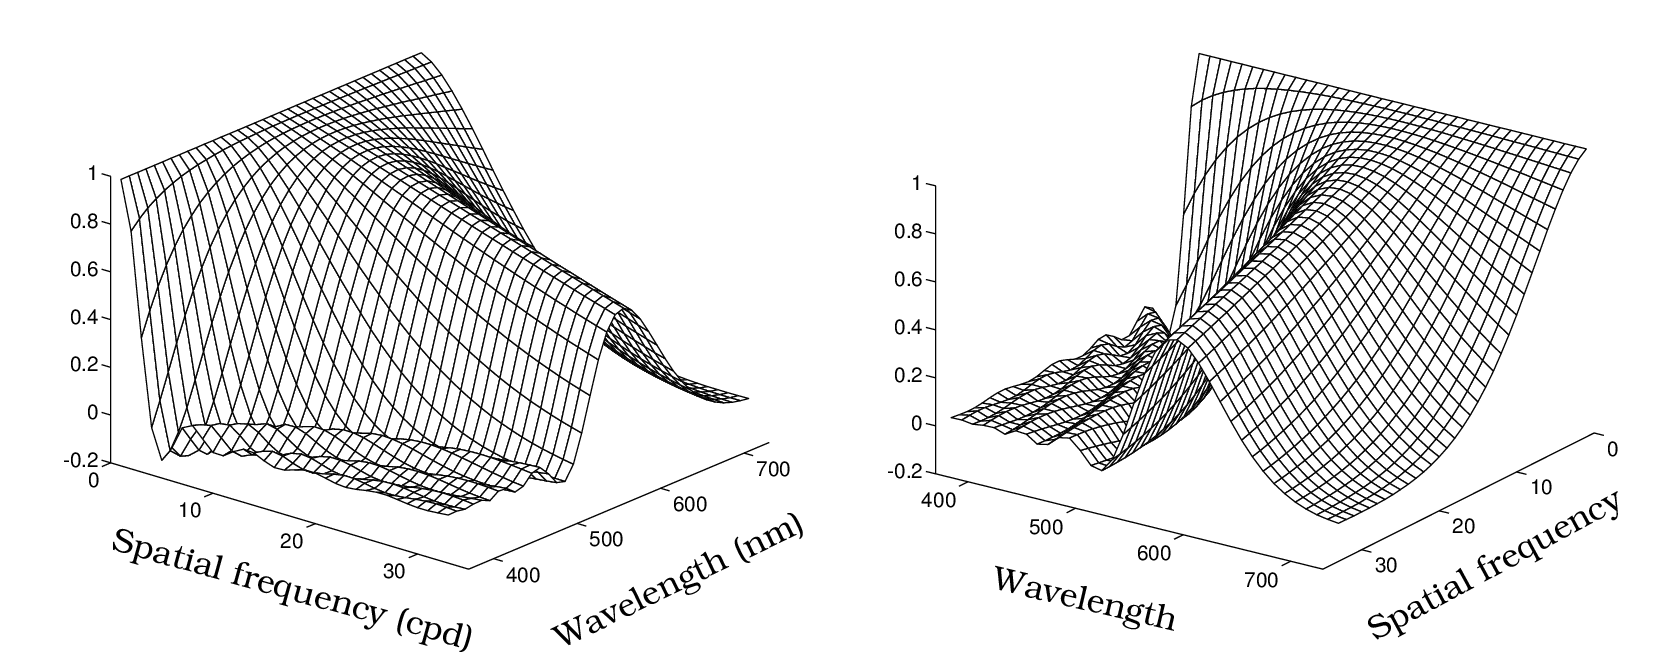
\includegraphics[width=0.7\textwidth,height=\textheight]{wp-content/uploads/2012/02/acOTF.png}

}

\caption{\label{fig-chromatic-aberration-otf}OTF of Chromatic
Aberration: Two views of the modulation transfer function of a model eye
at various wavelengths. The model eye has the same chromatic aberration
as the human eye (Figure~\ref{fig-chromatic-aberration}) and a 3.0mm
pupil diameter. The eye is in focus at 580nm; the curve at 580nm is
diffraction limited. The retinal image has no contrast beyond four
cycles per degree at short wavelengths.(From Marimont and Wandell
(1993)).}

\end{figure}%

The retinal image contains very poor spatial information at wavelengths
that are far from the best plane of focus. By accommodation, the human
eye can place any wavelength into good focus, but it is impossible to
focus all wavelengths simultaneously\footnote{A possible method of
  improving the spatial resolution of the eye to different wavelengths
  of light is to place the different classes of photoreceptors in
  slightly different image planes. Ahnelt et al. (1987) and Curcio et
  al. (1991) have observed that the short-wavelength photoreceptors have
  a slightly different shape and length from the middle- and
  long-wavelength photoreceptors. In principle, this difference could
  play a role to compensate for the chromatic aberration of the eye.
  But, the difference is very small, and it is unlikely that it plays
  any significant role in correcting for axial chromatic aberration.}.

\chapter{The Photoreceptor Mosaic}\label{sec-photoreceptor-mosaic}

In Chapter~\ref{sec-image-formation} we reviewed Campbell and Gubisch
(1966) measurements of the optical linespread function. Their data are
presented in Figure~\ref{fig-imgfor-cg-data}, as smooth curves, but the
actual measurements must have taken place at a series of finely spaced
intervals called sample points. In designing their experiment, Campbell
and Gubisch must have considered carefully how to space their sample
points because they wanted to space their measurement samples only
finely enough to capture the intensity variations in the measurement
plane. Had they positioned their samples too widely, then they would
have missed significant variations in the data. On the other hand,
spacing the sample positions too closely would have made the measurement
process wasteful of time and resources.

Just as Campbell and Gubisch sampled their linespread measurements, so
too the retinal image is sampled by the nervous system. Since only those
portions of the retinal image that stimulate the visual photoreceptors
can influence vision, the sample positions are determined by the
positions of the photoreceptors. If the photoreceptors are spaced too
widely, the image encoding will miss significant variation present in
the retinal image. On the other hand, if the photoreceptors are spaced
very close to one another compared to the spatial variation that is
possible given the inevitable optical blurring, then the image encoding
will be redundant, using more neurons than necessary to do the job. In
this chapter we will consider how the spatial arrangement of the
photoreceptors, called the photoreceptor mosaic, limits our ability to
infer the spatial pattern of light intensity present in the retinal
image.

We will consider separately the photoreceptor mosaics of each of the
different types of photoreceptors. There are two fundamentally different
types of photoreceptors in our eye, the rods and the cones. There are
approximately 5 million cones and 100 million rods in each eye. The
positions of these two types of photoreceptors differ in many ways
across the retina. Figure~\ref{fig-rod-cone-distribution} shows how the
relative densities of cone photoreceptors and rod photoreceptors vary
across the retina.

\begin{figure}

\centering{

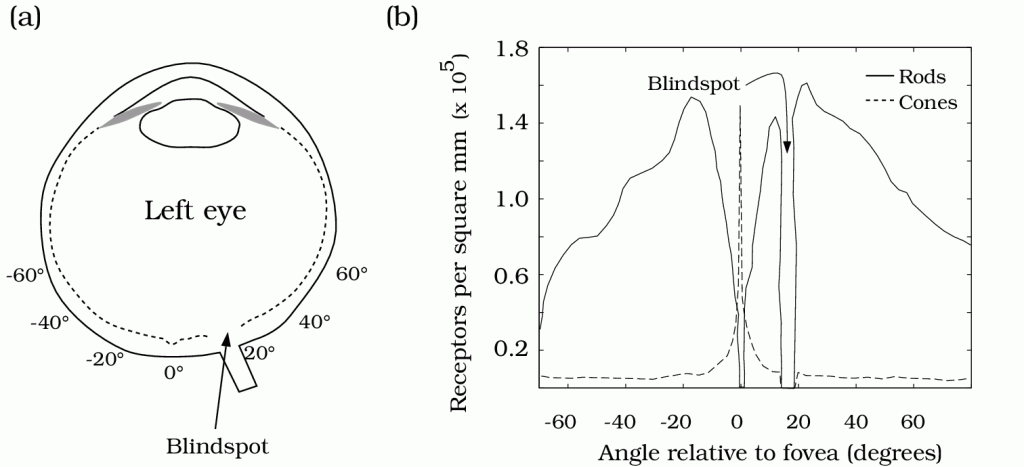
\includegraphics[width=0.7\textwidth,height=\textheight]{wp-content/uploads/2012/02/rod.cone_.distribution2-1024x467.png}

}

\caption{\label{fig-rod-cone-distribution}The distribution of rod and
cone photorceptors across the human retina. (a) The density of the
receptors is shown in degrees of visual angle relative to the position
of the fovea for the left eye. (b) The cone receptors are concentrated
in the fovea. The rod photoreceptors are absent from the fovea and reach
their highest density 10 to 20 degrees peripheral to the fovea. No
photoreceptors are present in the blindspot.}

\end{figure}%

The rods initiate vision under low illumination levels, called scotopic
light levels, while the cones initiate vision under higher, photopic
light levels. The range of intensities in which both rods and cones can
initiate vision is called mesopic intensity levels. At most wavelengths
of light, the cones are less sensitive to light than the rods. This
sensitivity difference, coupled with the fact that there are no rods in
the fovea, explains why we can not see very dim sources, such as weak
starlight, when we fixate our fovea directly on them. These sources are
too dim to be visible through the all cone fovea. The dim source only
becomes visible when it is placed in the periphery and be detected by
the rods. Rods are very sensitive light detectors: they generate a
detectable photocurrent response when they absorb a single photon of
light (Hecht et al. (1942); Schwartz (1977); Baylor (1987)).

The region of highest visual acuity in the human retina is the
\emph{fovea}. As Figure~\ref{fig-rod-cone-distribution} shows, the fovea
contains no rods, but it does contain the highest concentration of
cones. There are approximately 50,000 cones in the human fovea. Since
there are no photoreceptors at the optic disk, where the ganglion cell
axons exit the retina, there is a blindspot in that region of the retina
Chapter~\ref{sec-retinal-representation}.

\begin{figure}

\centering{

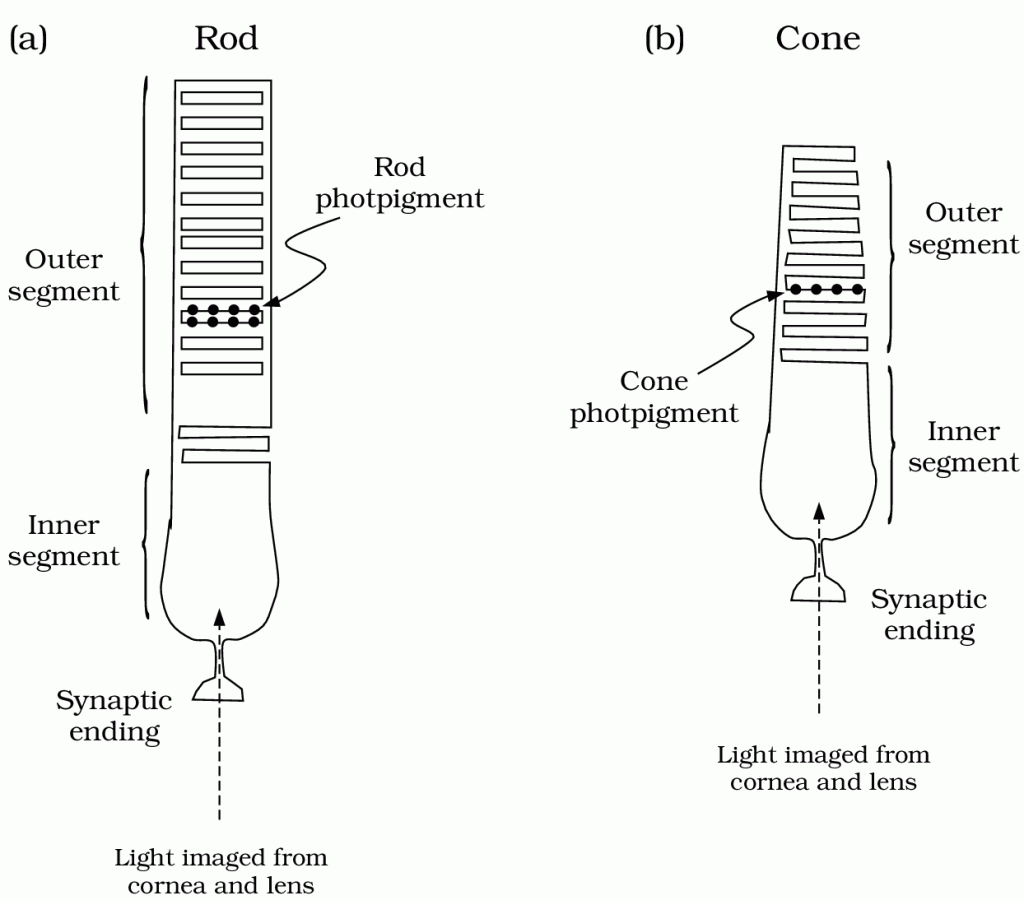
\includegraphics[width=0.6\textwidth,height=\textheight]{wp-content/uploads/2012/02/photoreceptor-1024x900.png}

}

\caption{\label{fig-photoreceptor}Mammalian rod and cone photoreceptors
contain the light absorbing pigment that initiates vision. Light enters
the photoreceptors through the inner segment and is funneled to the
outer segment that contains the photopigment. (After Baylor (1987))}

\end{figure}%

Figure~\ref{fig-photoreceptor} shows schematics of a mammalian rod and a
cone photoreceptor. Light imaged by the cornea and lens is shown
entering the receptors through the \emph{inner segments}. The light
passes into the \emph{outer segment} which contain light absorbing
\emph{photopigments}. As light passes from the inner to the outer
segment of the photoreceptor, it will either be absorbed by one of the
photopigment molecules in the outer segment or it will simply continue
through the photoreceptor and exit out the other side. Some light imaged
by the optics will pass between the photoreceptors. Overall, less than
ten percent of the light entering the eye is absorbed by the
photoreceptor photopigments (Baylor (1987)).

The rod photoreceptors contain a photopigment called rhodopsin. The rods
are small, there are many of them, and they sample the retinal image
very finely. Yet, visual acuity under scotopic viewing conditions is
very poor compared to visual acuity under photopic conditions. The
reason for this is that the signals from many rods converge onto a
single neuron within the retina, so that there is a many-to-one
relationship between rod receptors and neurons in the optic nerve
fibers. The density of rods and the convergence of their signals onto
single neurons improves the sensitivity of rod-initiated vision. Hence,
rod-initiated vision does not resolve fine spatial detail.

The foveal cone signals do not converge onto single neurons. Instead,
several neurons encode the signal from each cone, so that there is a
one-to-many relationship between the foveal cones and optic tract
neurons. The dense representation of the foveal cones suggests that the
spatial sampling of the cones must be an important aspect of the visual
encoding.

There are three types of cone photoreceptors within the human retina.
Each cone can be classified based on the wavelength sensitivity of the
photopigment in its outer segment. Estimates of the spectral sensitivity
of the three types of cone photoreceptors are shown in
Figure~\ref{fig-cone-spectra}. These curves are measured from the
cornea, so they include light loss due to the cornea, lens and inert
materials of the eye. In the next chapter we will study how color vision
depends upon the differences in wavelength selectivity of the three
types of cones. Throughout this book I will refer to the three types of
photoreceptors as the L, M and S cones.

(The letters refer to \textbf{L}ong-wavelength,
\textbf{M}iddle-wavelength and \textbf{S}hort-wavelength peak
sensitivity.)

\begin{figure}

\centering{

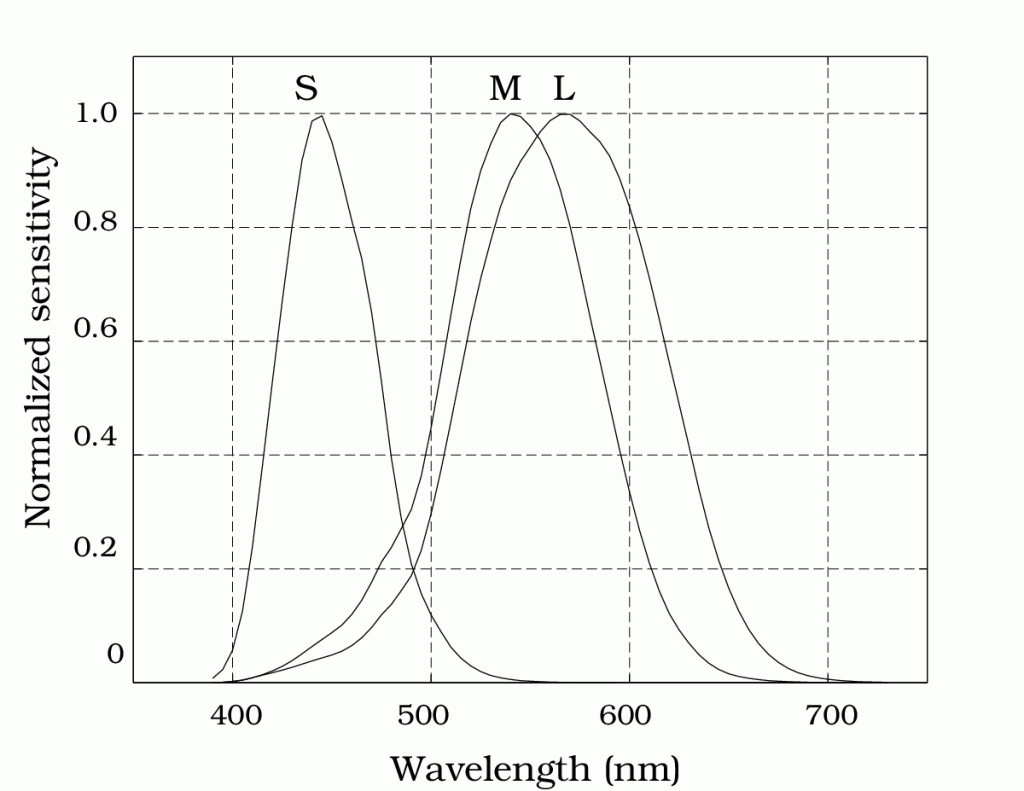
\includegraphics[width=0.5\textwidth,height=\textheight]{wp-content/uploads/2012/02/rec.spec_.sens_-1024x791.png}

}

\caption{\label{fig-cone-spectra}Spectral sensitivities of the L, M and
S cones in the human eye. The measurements are based on a light source
at the cornea, so that the wavelength loss due to the cornea, lens and
other inert pigments of the eye play a role in determining the
sensitivity. (Source: Stockman et al. (1993)).}

\end{figure}%

\begin{figure}

\centering{

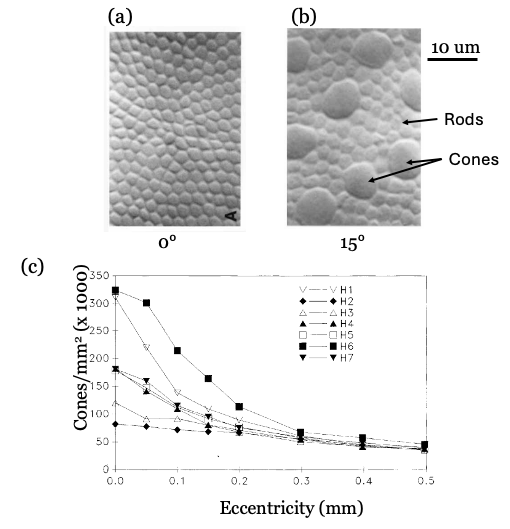
\includegraphics[width=0.8\textwidth,height=\textheight]{wp-content/uploads/2012/02/coneMosaic1-updated.png}

}

\caption{\label{fig-cone-mosaic}Photoreceptor Sampling: The spatial
mosaic of the human cones. A cross-section of the human retina at the
level of the inner segments. Cones in the fovea (a) are smaller than
cones in the periphery (b). As the separation between cones grows, the
rod receptors fill in the spaces. (c) The cone density varies with
distance from the fovea. Cone density is plotted as a function of
eccentricity for seven human retinae (After Curcio and Allen (1990)).}

\end{figure}%

Because light is absorbed after passing through the inner segment, the
position of the inner segment determines the spatial sampling position
of the photoreceptor. Figure~\ref{fig-cone-mosaic} shows cross-sections
of the human cone photoreceptors at the level of the inner segment in
the human fovea (part a) and just outside the fovea (part b). In the
fovea, cross-section shows that the inner segments are very tightly
packed and form a regular sampling array. A cross-section just outside
the fovea shows that the rod photoreceptors fill the spaces between the
cones and disrupt the regular packing arrangement. The scale bar
represents \(10~\mu\text{m}\); the cone photoreceptor inner segments in
the fovea are approximately \(2.3~\mu\text{m}\) wide with a minimum
center to center spacing of about \(2.5~\mu\text{m}\).
Figure~\ref{fig-cone-mosaic} (c) shows plots of the cone densities from
several different human retinae as a function of the distance from the
foveal center. The cone density varies across individuals.

\begin{figure}

\centering{

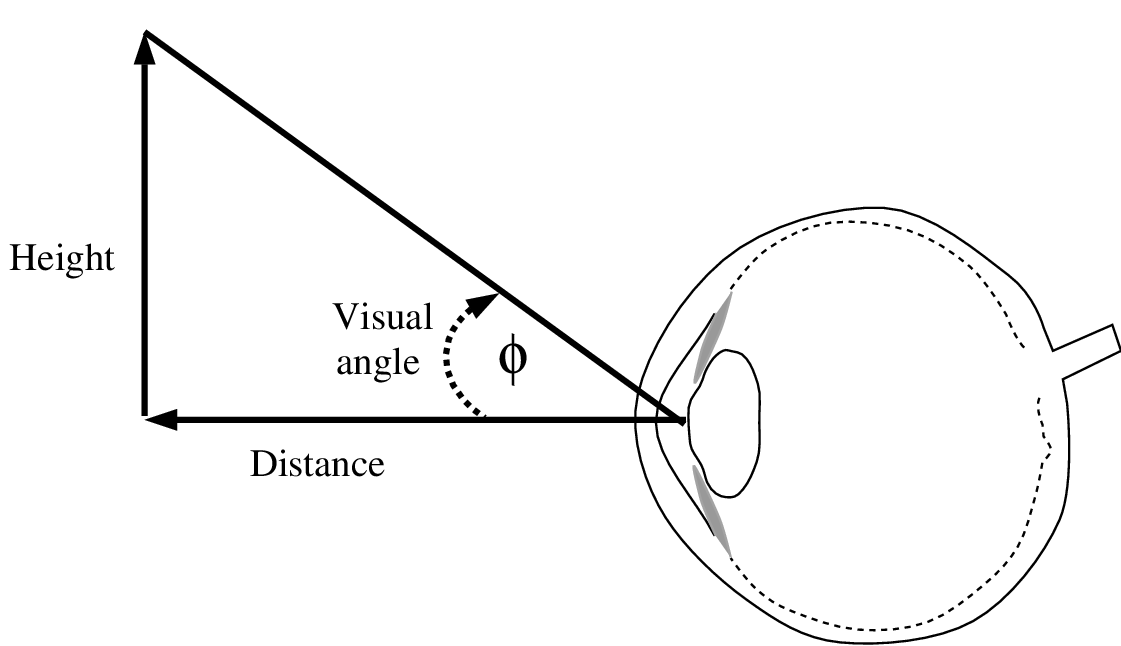
\includegraphics[width=0.5\textwidth,height=\textheight]{wp-content/uploads/2012/02/viewingangle.png}

}

\caption{\label{fig-viewing-angle}Calculating Viewing Angle: By
trigonometry, the tangent of the viewing angle, \(\phi\), is equal to
the ratio of height to distance in the right triangle shown. Therefore,
\(\phi\) is the inverse tangent of that ratio
(Equation~\ref{eq-viewingangle}).}

\end{figure}%

\subsection{Units of Visual Angle}\label{units-of-visual-angle}

We can convert these cone sizes and separations into degrees of visual
angle as follows. The distance from the effective center of of the eye's
optics to the retina is \(1.7 \times 10^{-2}~\mathrm{m}\) (17 mm). We
compute the visual angle spanned by one cone, \(\phi\), from the
trigonometric relationship in Figure~\ref{fig-viewing-angle}: the
tangent of an angle in a right triangle is equal to the ratio of the
lengths of the sides opposite and adjacent to the angle. This leads to
the following equation:

\begin{equation}\phantomsection\label{eq-viewingangle}{
\tan(\phi) = \frac{2.5 \times 10^{-6}~\mathrm{m}}{1.7 \times 10^{-2}~\mathrm{m}} = 1.47 \times 10^{-4}
}\end{equation}

The width of a cone in degrees of visual angle, \(\phi\), is
approximately \(0.0084\) degrees, or roughly one-half minute of visual
angle. In the center of the eye, then, where the photoreceptors are
packed densely, the cone photoreceptors are tightly packed and their
centers are separated by one-half minute of visual angle.

\section{The S Cone Mosaic}\label{sec-s-cone-mosaic}

\subsection{Behavioral Measurements}\label{sec-s-cone-behavior}

Just as the rods and cones have different spatial sampling
distributions, so too the three types of cone photoreceptors have
different spatial sampling distributions. The sampling distribution of
the short-wavelength cones was the first to be measured empirically, and
it has been measured both with behavioral and physiological methods. The
behavioral experiments were carried out as part of D. Williams
dissertation at the University of California in San Diego. Williams et
al. (1981) took advantage of several features of the short-wavelength
photoreceptors. As background to their work, we first describe several
features of the photoreceptors.

The photopigment in the short-wavelength photoreceptors is significantly
different from the photopigment in the other two types of
photoreceptors. Notice that the wavelength sensitivity of the L and M
photopigments are very nearly the same (Figure~\ref{fig-cone-spectra}).
The sensitivity of the S photopigment is significantly higher in the
short-wavelength part of the spectrum than the sensitivity of the other
two photopigments. As a result, if we present the visual system with a
very weak light, containing energy only in the short-wavelength portion
of the spectrum, the S cones will absorb relatively more quanta than the
other two classes. Indeed, the discrepancy in the absorptions is so
large that it is reasonable to suppose that when short-wavelength light
is barely visible, at detection threshold, perception is initiated
uniquely from a signal that originates in the short-wavelength
receptors.

We can give the short-wavelength receptors an even greater sensitivity
advantage by presenting a blue test target on a steady yellow
background. As we will discuss in later chapters, steady backgrounds
suppress visual sensitivity. By using a yellow background, we can
suppress the sensitivity of the \(\mathrm{L}\) and \(\mathrm{M}\) cones
and the rods and yet spare the sensitivity of the \(\mathrm{S}\) cones.
This improves the relative sensitivity advantage of the short-wavelength
receptors in detecting the short-wavelength test light. It is reasonable
to suppose that when short-wavelength light is barely visible, at
detection threshold, perception is initiated uniquely from a signal that
originates in the short-wavelength receptors.

During the experiment, the subjects visually fixated on a small mark.
They were then presented with short-wavelength test lights that were
likely to be seen with a signal initiated by the \(\mathrm{S}\) cones.
After the eye was perfectly fixated, the subject pressed a button and
initiated a stimulus presentation. The test stimulus was a tiny point of
light, presented very briefly (10 ms). The test light was presented at
different points in the visual field. If light from the short-wavelength
test fell upon a region that contained \(\mathrm{S}\) cones, sensitivity
should be relatively high. On the other hand, if that region of the
retina contained no \(\mathrm{S}\) cones, sensitivity should be rather
low. Hence, from the spatial pattern of visual sensitivity, Williams,
Hayhoe and Macleod inferred the spacing of the \(\mathrm{S}\) cones.

\begin{figure}

\centering{

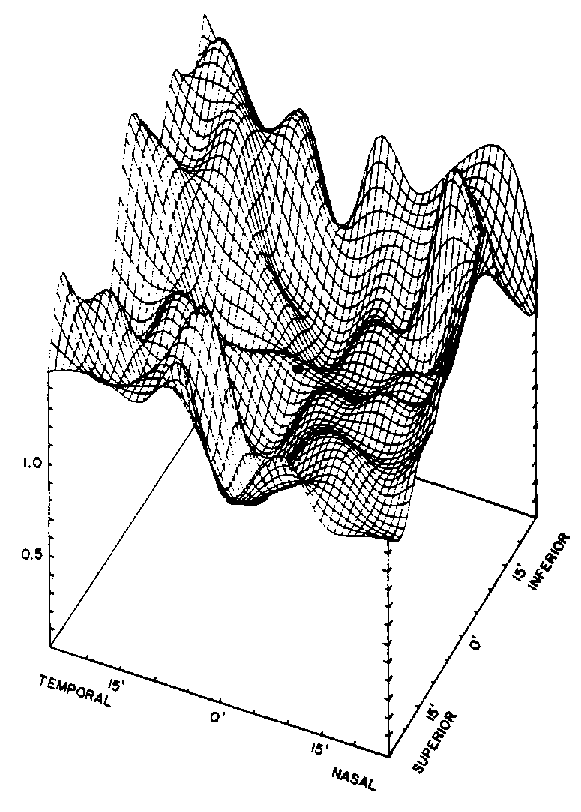
\includegraphics[width=0.5\textwidth,height=\textheight]{wp-content/uploads/2012/02/williams.dat_6.png}

}

\caption{\label{fig-s-cone-mosaic}Short-wavelength Cone Mosaic:
Psychophysical estimate of the spatial mosaic of the S cones. The height
of the surface represents the observer's threshold sensitivity to a
short wavelength test light presented on a yellow background. The test
was presented at a series of locations spanning a grid around the fovea
(black dot). The peaks in sensitivity probably correspond to the
positions of the S cones. (From Williams et al. (1981)).}

\end{figure}%

The sensitivity measurements are shown in
Figure~\ref{fig-s-cone-mosaic}. First, notice that in the very center of
the visual field, in the central fovea, there is a large valley of low
sensitivity. In this region, there appear to be no short-wavelength
cones at all. Second, beginning about half a degree from the center of
the visual field there are small, punctate spatial regions of high
sensitivity. We interpret these results by assuming that these peaks
correspond to the positions of this observer's \(\mathrm{S}\) cones. The
gaps in between, where the observer has rather low sensitivity are
likely to be patches of \(\mathrm{L}\) and \(\mathrm{M}\) cones. Around
the central fovea, the typical separation between the inferred
\(\mathrm{S}\) cones is about 8 to 12 minutes of visual angle. Thus,
there are five to seven \(\mathrm{S}\) cones per degree of visual angle.

\subsection{Biological Measurements}\label{sec-s-cone-biology}

There have been several biological measurements of the short-wavelength
cone mosaic, and we can compare these with the behavioral measurements.
Marc and Sperling (1977) used a stain that is taken up by cones when
they are active. They applied this stain to a baboon retina and then
stimulated the retina with short-wavelength light in the hopes of
staining only the short-wavelength receptors. They found that only a few
cones were stained when the stimulus was a short-wavelength light. The
typical separation between the stained cones was about 6 minutes of arc.
This value is smaller than the separation that Williams et al. (1981)
observed and may be a species-related difference.

Monasterio et al. (1981) discovered that when the dye procion yellow is
applied to the retina, the dye is absorbed in the outer segments of all
the photoreceptors, but it stains only a small subset of the
photoreceptors completely. Figure~\ref{fig-blue-cone-mosaic} shows a
group of stained photoreceptors in cross-section.

The indirect arguments identifying these special cones as \(\mathrm{S}\)
cones are rather compelling. But, a more certain procedure was developed
by C. Curcio and her colleagues. They used a biological marker,
developed based on knowledge of the genetic code for the \(\mathrm{S}\)
cone photopigment, to label selectively the \(\mathrm{S}\) cones in the
human retina (Curcio et al. (1991)). Their measurements agree well
quantitatively with Williams' psychophysical measurements, namely that
the average spacing between the \(\mathrm{S}\) cones is 10 minutes of
visual angle. Curcio and her colleagues could also confirm some early
anatomical observations that the size and shape of the \(\mathrm{S}\)
cones differ slightly from the \(\mathrm{L}\) and \(\mathrm{M}\) cones.
The \(\mathrm{S}\) cones have a wider inner segment, and they appear to
be inserted within an orderly sampling arrangement of their own between
the sampling mosaics of the other two cone types (Ahnelt et al. (1987)).

\subsection{Why are the S cones widely
spaced?}\label{sec-s-cones-widely-spaced}

The spacing between the \(\mathrm{S}\) cones is much larger than the
spacing between the \(\mathrm{L}\) and \(\mathrm{M}\) cones. Why should
this be? The large spacing between the \(\mathrm{S}\) cones is
consistent with the strong blurring of the short-wavelength component of
the image due to the axial chromatic aberration of the lens. Recall that
axial chromatic aberration of the lens blurs the short-wavelength
portion of the retinal image, the part \(\mathrm{S}\) cones are
particularly sensitive to, more than the middle- and long-wavelength
portion of the image (Figure~\ref{fig-chromatic-aberration}). In fact,
under normal viewing conditions the retinal image of a fine line at 450
nm falls to one half its peak intensity nearly 10 minutes of visual
angle away from the location of its peak intensity. At that wavelength,
the retinal image only contains significant contrast at spatial
frequency components below 3 cycles per degree of visual angle. The
optical defocus force the wavelength components of the retinal image the
\(\mathrm{S}\) cones encode to vary smoothly across space. Consequently,
the \(\mathrm{S}\) cones can sample the image only six times per degree
and still recover the spatial variation passed by the cornea and lens.

\begin{figure}

\centering{

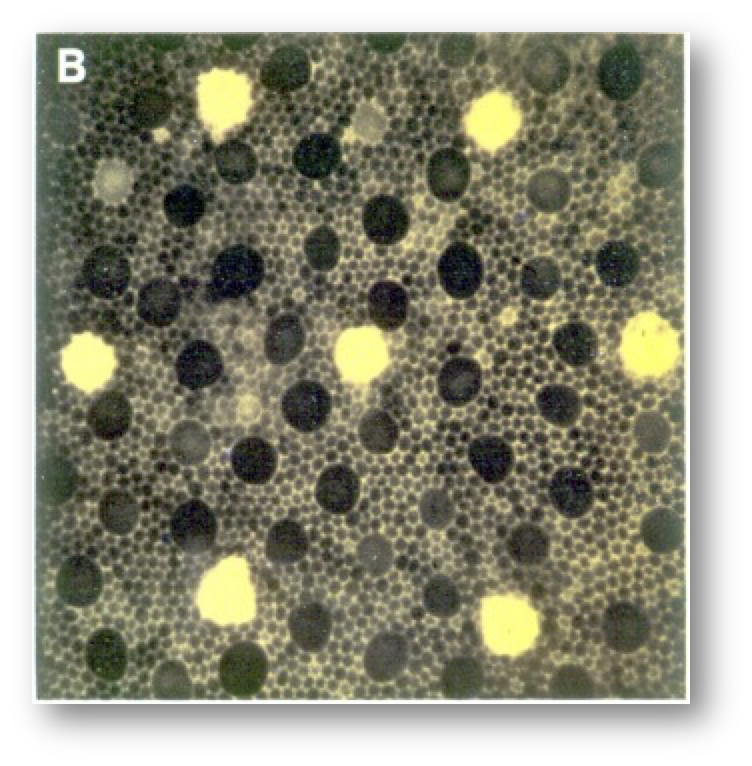
\includegraphics[width=0.7\textwidth,height=\textheight]{wp-content/uploads/2012/02/blueConeMosaic-updated.png}

}

\caption{\label{fig-blue-cone-mosaic}Short-Wavelength Cone Mosaic:
Procion Yellow Stains. Biological estimate of the spatial mosaic of the
\(S\) cones in the macaque retina. A small fraction of the cones absorb
the procion yellow stain; these are shown as the dark spots in this
image. These cones, thought to be the\(S\) cones, are shown in a
cross-section through the inner segment layer of the retina. (From
Monasterio et al. (1981))}

\end{figure}%

Interestingly, the \emph{spatial} defocus of the short-wavelength
component of the image also implies that signals initiated by the
\(\mathrm{S}\) cones will vary slowly over \emph{time}. In natural
scenes, temporal variation occurs mainly because of movement of the
observer or an object. When a sharp boundary moves across a cone
position, the light intensity changes rapidly at that point. But, if the
boundary is blurred, changing gradually over space, then the light
intensity changes more slowly. Since the short-wavelength signal is
blurred by the optics, and temporal variation is mainly due to motion of
objects, the \(\mathrm{S}\) cones will generally be coding slower
temporal variations than the \(\mathrm{L}\) and \(\mathrm{M}\) cones.

At the very earliest stages of vision, we see that the properties of
different components of the visual pathway fit smoothly together. The
optics set an important limit on visual acuity, and the \(\mathrm{S}\)
cone sampling mosaic can be understood as a consequence of the optical
limitations. As we shall see, the \(\mathrm{L}\) and \(\mathrm{M}\) cone
mosaic densities also make sense in terms of the optical quality of the
eye.

This explanation of the \(\mathrm{S}\) cone mosaic flows from our
assumption that visual acuity is the main factor governing the
photoreceptor mosaic. For the visual streams initiated by the cones,
this is a reasonable assumption. There are other important factors,
however, that can play a role in the design of a visual pathway. For
example, acuity is not the dominant factor in the visual stream
initiated by rod vision. In principle the resolution available in the
rod encoding is comparable to the acuity available in the cone
responses; but, visual acuity using rod-initiated signals is very poor
compared to acuity using cone-initiated signals. Hence, we shouldn't
think of the rod sampling mosaic in terms of visual acuity. Instead, the
high density of the rods and their convergence onto individual neurons
suggests that we think of the imperative of rod-initiated vision in
terms of improving the signal-to-noise under low light levels. In the
rod-initiated signals, the visual system trades visual acuity for an
increase in the signal-to-noise ratio. In the earliest stages of the
visual pathways, then, we can see structure, function and design
criteria coming together.

When we ask why the visual system has a particular property, we need to
relate observations from the different disciplines that make up vision
science. Questions about anatomy require us to think about the behavior
the anatomical structure serves. Similarly, behavior must be explained
in terms of algorithms and the anatomical and physiological responses of
the visual pathway. By considering the visual pathways from multiple
points of view, we piece together a complete picture of how system
functions.

\section{Visual Interferometry}\label{sec-interferometry}

\begin{figure}

\centering{

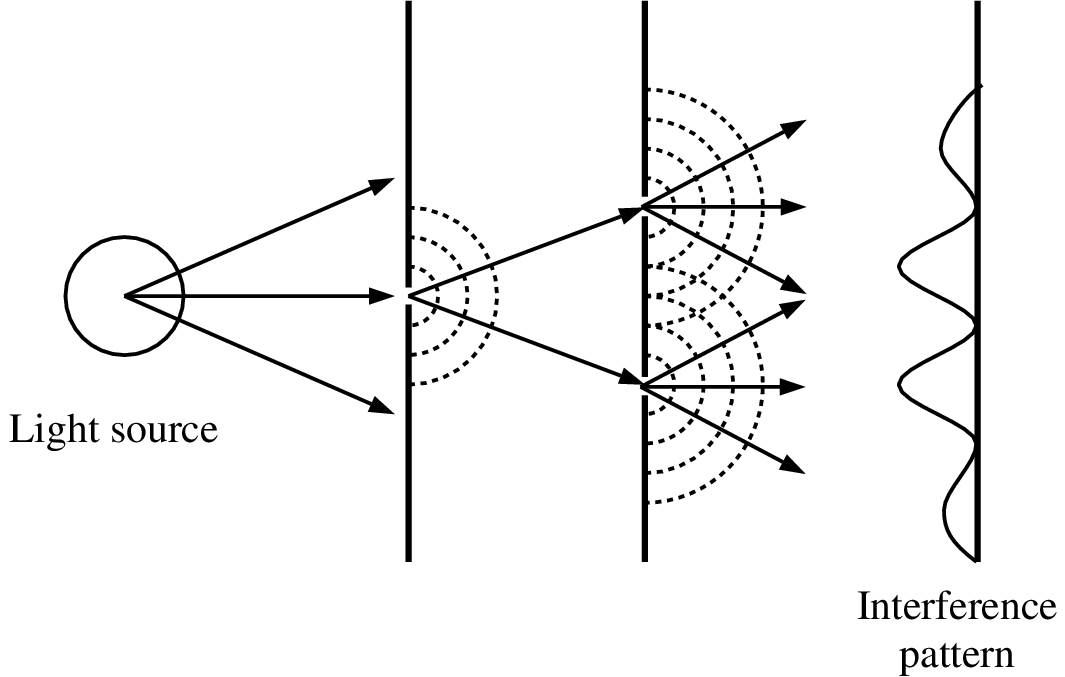
\includegraphics[width=0.6\textwidth,height=\textheight]{wp-content/uploads/2012/02/Young-doubleslit.png}

}

\caption{\label{fig-young-double-slit}Young's double-slit experiment
uses a pair of coherent light sources to create an interference pattern
of light. The intensity of the resulting image is nearly sinusoidal, and
its spatial frequency depends upon the spacing between the two slits.}

\end{figure}%

Thomas Young, the brilliant scientist, physician, and classicist
demonstrated to the Royal Society that when two beams of coherent light
generate an image on a surface such as the retinal surface, the
resulting image is an interference pattern Young (1804). His experiment
is often called the \emph{double-slit} or \emph{double-pinhole}
experiment. Using an ordinary light source, Young passed the light
through a small pinhole first and then through a pair of slits, as
illustrated in Figure~\ref{fig-interferometer}. In the experiment, the
first pinhole serves as the source of light; the double pinholes then
pass the light from the common original source. Because they share this
common source, light emitted from the double pinholes are in a coherent
phase relationship and their wavefronts interfere with one another. This
interference results in an image that varies nearly sinusoidally in
intensity.

\begin{figure}

\centering{

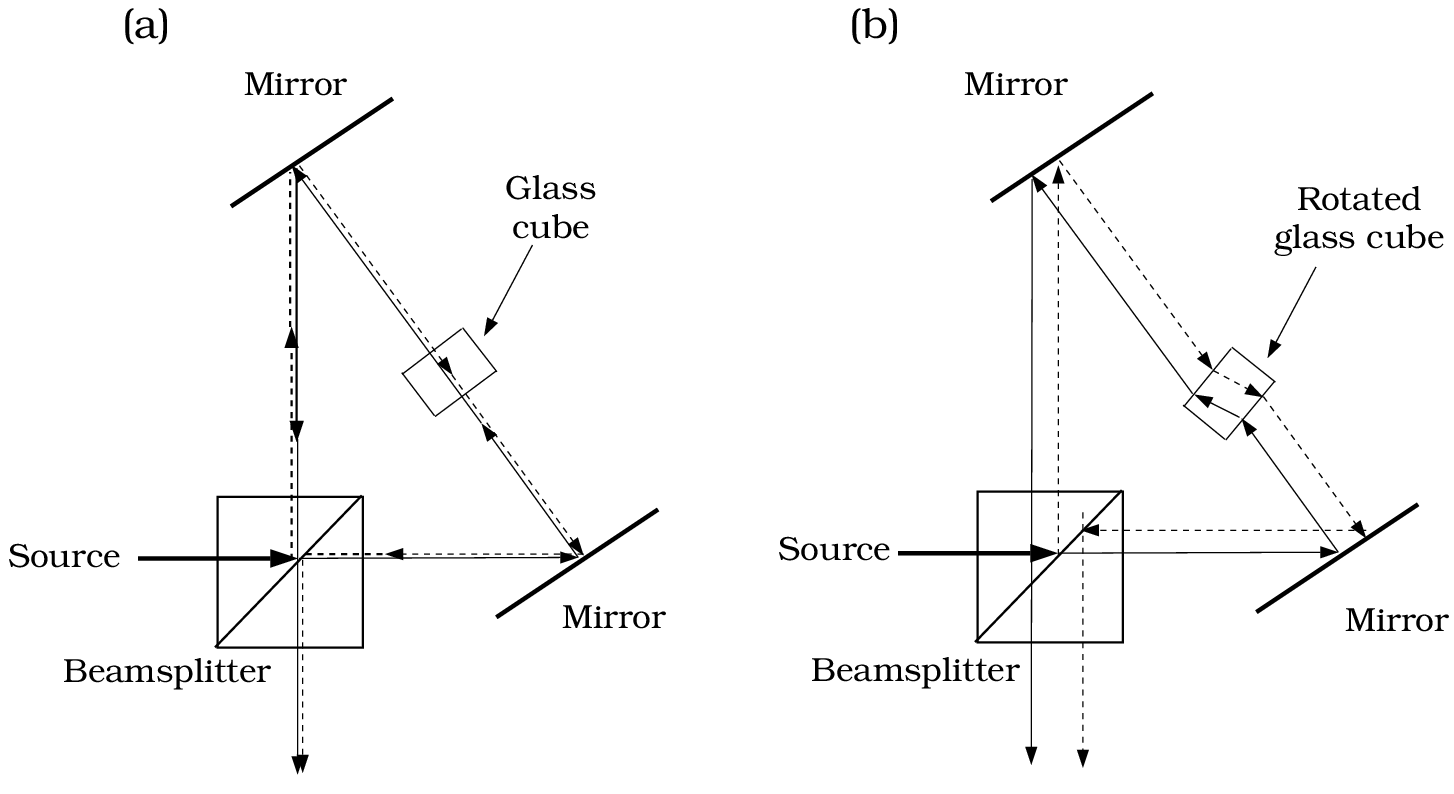
\includegraphics[width=0.6\textwidth,height=\textheight]{wp-content/uploads/2012/02/interferometer.png}

}

\caption{\label{fig-interferometer}A visual interferometer creates an
interference pattern as in Young's double-slit experiment. In the device
shown here the original beam is split into two paths shown as the solid
and dashed lines. (a) When the glass cube is at right angles to the
light path, the two beams traverse an equal path and are imaged at the
same point after exiting the interferometer. (b) When the glass is
rotated, the two beams traverse slightly different paths causing the
images of the two coherent beams to be displaced and thus create an
interference pattern. (After Macleod et al. (1992)).}

\end{figure}%

We can also achieve this narrow pinhole effect by using a laser as the
original source. The key elements of a visual interferometer used by
Macleod et al. (1992) are shown in Figure~\ref{fig-interferometer}.
Light from a laser enters the beamsplitter and is divided into one part
that continues along a straight path (solid line) and a second path that
is reflected along a path to the right (dashed line). These two beams,
originating from a common source, will be the pair of sources to create
the interference pattern on the retina.

Light from each beam is reflected from a mirror towards a glass cube. By
varying the orientation of the glass cube, the experimenter can vary the
path of the two beams. When the glass cube is at right angles to the
light path, as is shown in part (a), the beams continue in a straight
path along opposite directions and emerge from the beamsplitter at the
same position. When the glass cube is rotated, as is shown in part (b),
the refraction due to the glass cube symmetrically changes the beam
paths; they emerge from the beamsplitter at slightly different locations
and act as a pair of point sources. This configuration creates two
coherent beams that act like the two slits in Thomas Young's experiment,
creating an interference pattern. The amount of rotation of the glass
cube controls the separation between the two beams.

Each beam passes through only a very small section of the cornea and
lens. The usual optical blurring mechanisms do not interfere with the
image formation, since the lens does not serve to converge the light
(see the section on lenses in Chapter~\ref{sec-image-formation}.
Instead, the pattern that is formed depends upon the diffraction due to
the restricted spatial region of the light source.

\begin{figure}

\centering{

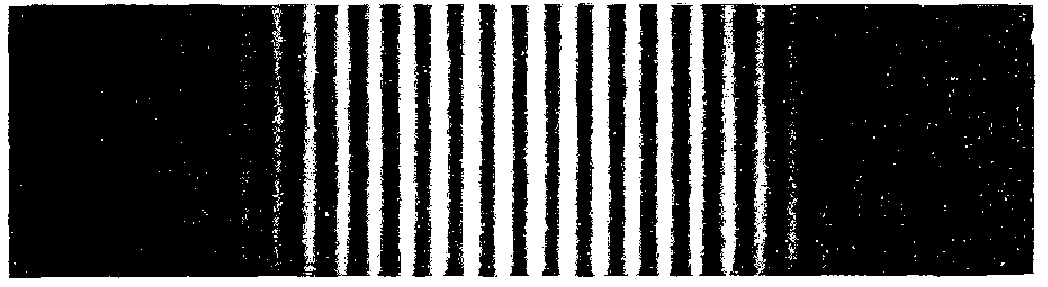
\includegraphics[width=0.6\textwidth,height=\textheight]{wp-content/uploads/2012/02/interference.sinusoid1.png}

}

\caption{\label{fig-interference-sinusoid}Sinusoidal Interference
Pattern. An interference pattern. The image was created using a
double-slit apparatus. The intensity of the pattern is nearly
sinusoidal. (From Jenkins and White (1937))}

\end{figure}%

We can use diffraction to create retinal images with much higher spatial
frequencies than are possible through ordinary optical imaging by the
cornea and lens. Figure~\ref{fig-interference-sinusoid} is an image of a
diffraction pattern created by a pair of two slits. The intensity of the
pattern is nearly a sinusoidal function of retinal position. The spatial
frequency of the retinal image can be controlled by varying the
separation between the focal points; the smaller the separation between
the slit, the lower the spatial frequency in the interference pattern.
Thus, by rotating the glass cube in the interferometer and changing the
separation of the two beams we can control the spatial frequency of the
retinal image.

Visual interferometry permits us to image fine spatial patterns at much
higher contrast than when we image these patterns using ordinary optical
methods. For example, Figure~\ref{fig-modulation-transfer} shows that a
\(60\) cycles per degree sinusoid cannot exceed \(10\%\) contrast when
imaged through the optics. Using a visual interferometer, we can present
patterns at frequencies considerably higher than \(60\) cycles per
degree at \(100\%\) contrast.

However, a challenge remains: the interferometric patterns are not fine
lines or points, but rather extended patterns (cosinusoids). Therefore,
we cannot use the same logic as Williams et al.~and map the receptors by
carefully positioning the stimulus. We need to think a little bit more
about how to use the cosinusoidal interferometric patterns to infer the
structure of the cone mosaic.

\section{Sampling and Aliasing}\label{sec-sampling-aliasing}

\begin{figure}

\centering{

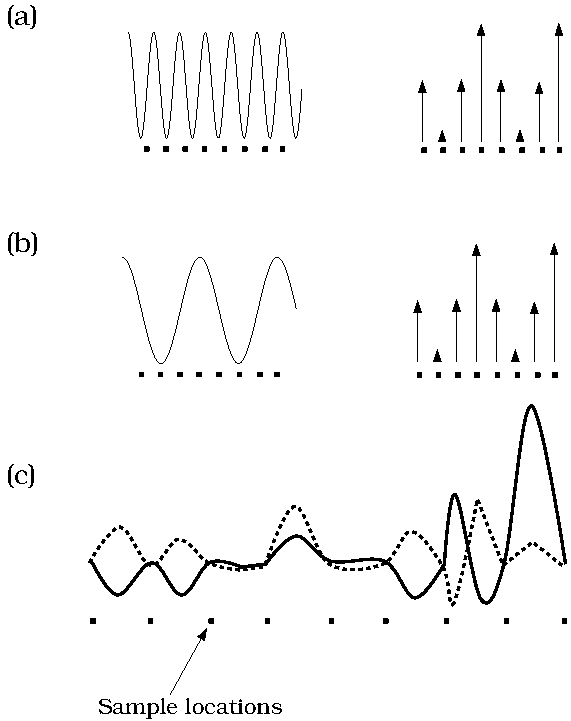
\includegraphics[width=0.6\textwidth,height=\textheight]{wp-content/uploads/2012/02/aliasing.png}

}

\caption{\label{fig-aliasing}Aliasing of signals results when sampled
values are the same but in-between values are not. (a,b) The continuous
sinusoids on the left have the same values at the sample positions
indicated by the black squares. The values of the two functions at the
sample positions are shown by the height of the stylized arrows on the
right. (c) Undersampling may cause us to confuse various functions, not
just sinusoids. The two curves at the bottom have the same values at the
sampled points, differing only in between the sample positions.}

\end{figure}%

The most basic observation concerning sampling and aliasing is this: we
can measure only that portion of the input signal that falls over the
sample positions. Figure~\ref{fig-aliasing} shows one-dimensional
examples of aliasing and sampling. Parts (a) and (b) contain two
different cosinusoidal signals (left) and the locations of the sample
points. The values of these two cosinusoids at the sample points are
shown by the height of the arrows on the right. Although the two
continuous cosinusoids are quite different, they have the same values at
the sample positions. Hence, if cones are only present at the sample
positions, the cone responses will not distinguish between these two
inputs. We say that these two continuous signals are an \emph{aliased}
pair. Aliased pairs of signals are indistinguishable after sampling.
Hence, sampling degrades our ability to discriminate between sinusoidal
signals.

Figure~\ref{fig-alias-example} shows that sampling degrades our ability
to discriminate between signals in general, not just between sinusoids.
Whenever two signals agree at the sample points, their sampled
representations agree. The basic phenomenon of aliasing is this: Signals
that only differ between the sample points are indistinguishable after
sampling.

\begin{figure}

\centering{

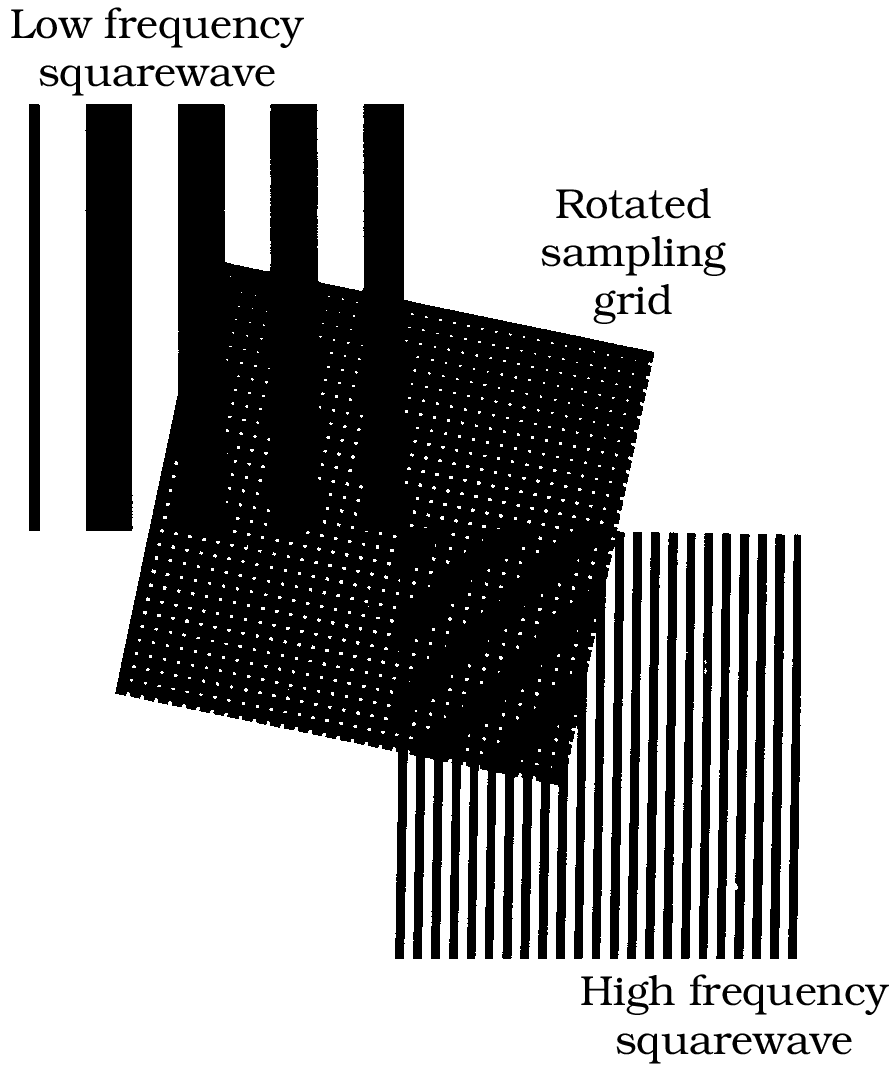
\includegraphics[width=0.6\textwidth,height=\textheight]{wp-content/uploads/2012/02/aliasExample.png}

}

\caption{\label{fig-alias-example}Square-wave aliasing. The squarewave
on top is seen accurately through the grid. The squarewave on the bottom
is at a higher spatial frequency than the grid sampling. When seen
through the grid, the pattern appears at a lower spatial frequency and
rotated.}

\end{figure}%

The exercises at the end of this chapter include some computer programs
that can help you make sampling demonstrations like the one in
Figure~\ref{fig-alias-example}. If you print out squarewave patterns and
various sampling arrays, using the programs provided, you can print
various patterns onto overhead transparencies and explore the effects of
sampling. Figure~\ref{fig-alias-example} shows an example of two
squarewave patterns seen through a sampling grid. After sampling, the
high frequency pattern appears to be a rotated, low frequency signal.

\subsection{Sampling is a Linear Operation}\label{sec-sampling-linear}

The sampling transformation takes the retinal image as input and
generates a portion of the retinal image as output. Sampling is a linear
operation as the following thought experiment reveals. Suppose we
measure the sample values at the cone positions when we present image
\(A\); call the intensities at the sample positions \(S(A)\). Now,
measure the intensities at the sample positions for a second image,
\(B\); call the sample intensities \(S(B)\). If we add together the two
images, the new image, \(A + B\), contains the sum of the intensities in
the original images. The values picked out by sampling will be the sum
of the two sample vectors, \(S(A) + S(B)\).

Since sampling is a linear transformation, we can express it as a matrix
multiplication. In our simple description, each position in the retinal
image either falls within a cone inner segment or not. The sampling
matrix consists of \(N\) rows representing the \(N\) sampled values.
Each row is all zero except at the entry corresponding to that row's
sampling position, where the value is \(1\).

\subsection{Aliasing of harmonic functions}\label{sec-aliasing-harmonic}

For uniform sampling arrays we have already observed that some pairs of
sinusoidal stimuli are aliases of one another (part (a) of
Figure~\ref{fig-aliasing}). We can analyze precisely which pairs of
sinusoids form alias pairs using a little bit of algebra. Suppose that
the continuous input signal is \(\cos ( 2 \pi f x )\). When we sample
the stimulus at regular intervals, the output values will be the value
of the cosinusoid at those regularly spaced sample points. Suppose that
within a single unit of distance there are \(N\) sample points, so that
our measurements of the stimulus takes place every \(1 / N\) units. Then
the sampled values will be
\(S_{f} ( k ) = \cos \left( 2 \pi f \frac{k}{N} \right)\). A second
cosinusoid, at frequency \(f'\) will be an alias if its sample values
are equal, that is, if \(S_{f'} (k) = S_{f} (k)\).

With a little trigonometry, we can prove that the sample values for any
pair of cosinusoids with frequencies \(\frac{N}{2} - f\) and
\(\frac{N}{2} + f\) will be equal. That is,

\begin{equation}\phantomsection\label{eq-cos-alias}{
\cos\left( 2\pi \left( \frac{N}{2} + f \right) \frac{k}{N} \right) = \cos\left( 2\pi \left( \frac{N}{2} - f \right) \frac{k}{N} \right)
}\end{equation}

(To prove this we must use the cosine addition law. The steps in the
verification are in Exercise 5 at the end of the chapter.)

The frequency \(f = N / 2\) is called the \emph{Nyquist frequency} of
the uniform sampling array; sometimes it is referred to as the
\emph{folding frequency}. Cosinusoidal stimuli whose frequencies differ
by equal amounts above and below the Nyquist frequency of a uniform
sampling array will have identical sample responses.

\subsection{Experimental Implications}\label{experimental-implications}

The aliasing calculations suggest an experimental method to measure the
spacing of the cones in the eye. If the cone spacing is uniform, then
pairs of stimuli separated by equal amounts above and below the Nyquist
frequency should appear indistinguishable. Specifically, a signal
\(\cos \left(2 \pi \left( \frac{N}{2} + f \right) \right)\) that is
above the Nyquist frequency will appear the same as the signal
\(\cos \left(2 \pi \left( \frac{N}{2} - f \right) \right)\) that is an
equal amount below the Nyquist frequency. Thus, as subjects view
interferometric patterns of increasing frequency, as we cross the
Nyquist frequency the perceived spatial frequency should begin to
decrease even though the physical spatial frequency of the diffraction
pattern increases.

Yellott (1982) examined the aliasing prediction in a nice graphical way.
He made a sampling grid from Polyak's (Polyak (1957)) anatomical
estimate of the cone positions. He simply poked small holes in the paper
at the cone positions in one of Polyak's anatomical drawings. We can
place any image we like, for example patterns of light and dark bars,
behind the grid. The bits of the image that we see are only those that
would be seen by the visual system. Any pair of images that differ only
in the regions between the holes will be an aliased pair. Yellott
introduced the method and proper analysis, but he used the Polyak (1957)
data on the outer segment positions rather than on the positions of the
inner segments (Miller and Bernard (1983)).

This experiment is relatively straightforward for the \(\mathbf{S}\)
cones. Since these cones are separated by about \(10\) minutes of visual
angle, there are about six \(\mathbf{S}\) cones per degree of visual
angle. Hence, their Nyquist frequency is \(3\) cycles per degree of
visual angle (cpd). It is possible to correct for chromatic aberration
and to present spatial patterns at these low frequencies through the
lens. Such experiments confirm the basic predictions that we will see
aliased patterns (Williams and Collier (1983)).

\section{The L and M Cone Mosaic}\label{sec-lm-mosaic}

Experiments using a visual interferometer to image a high frequency
pattern at high contrast on the retina are a powerful way to analyze the
sampling mosaic of \(\mathrm{L}\) and \(\mathrm{M}\) cones. But, even
before this was technical feat was possible, Helmholtz' (Helmholtz
(1866/1911)) noticed that extremely fine patterns, looked at without any
special apparatus, can appear wavy. He attributed this observation to
sampling by the cone mosaic. His perception of a fine pattern and his
graphical explanation of the waviness in terms of cone sampling are
shown in part (a) of Figure~\ref{fig-alias-drawings} (boxed drawings).

\begin{figure}

\centering{

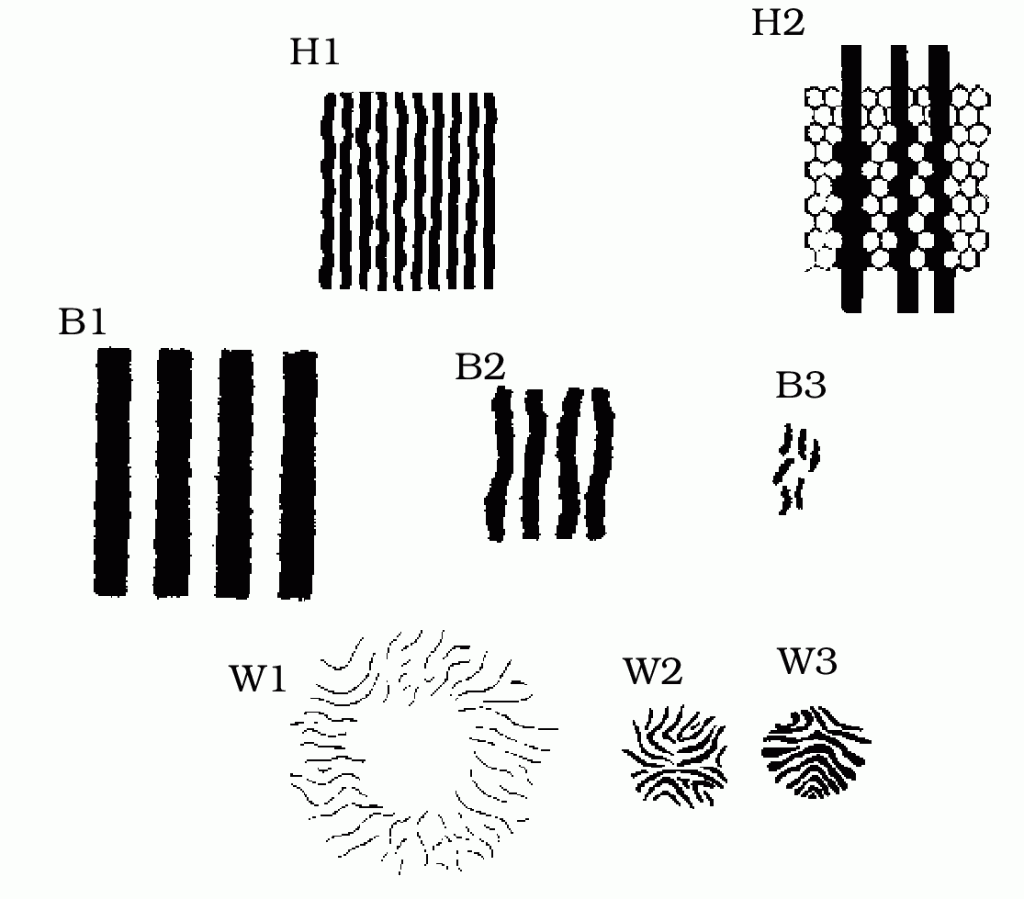
\includegraphics[width=0.6\textwidth,height=\textheight]{wp-content/uploads/2012/02/aliasDrawings-1024x899.png}

}

\caption{\label{fig-alias-drawings}Drawings of perceived aliasing
patterns by several different observers. Helmholtz' observed aliasing of
fine patterns which he drew in part H1. He offered an explanation of his
observations, in terms of cone sampling, in H2 (Helmholtz (1866/1911)).
The Byram (1944) drawings of three interference patterns at 40, 85 and
150 cpd are labeled B1, B2, and B3. Drawings W1,W2 and W3 are by
subjects in Williams' laboratory who drew their impression of aliasing
of an 80 cpd and two patterns at 110 cpd (williams1985b-aliasing)}

\end{figure}%

G. Byram was the first to describe the appearance of high frequency
interference gratings (Byram (1944)). His drawings of the appearance of
these patterns are shown in part (b) of the figure. The image on the
left shows the appearance of a low frequency pattern diffraction
pattern. The apparent spatial frequency of this stimulus is faithful to
the stimulus. Byram noted that as the spatial frequency increases
towards 60 cpd, the pattern still appears to be a set of fine lines, but
they are difficult to see (middle drawing). When the pattern
significantly exceeds the Nyquist frequency, it becomes visible again
but looks like the low-frequency pattern drawn on the right. Further, he
reports that the pattern shimmers and is unstable, probably due to the
motion of the pattern with respect to the cone mosaic (Byram (1944),
Williams (1985a)).

Over the last 10 years D. Williams' group has replicated and extended
these measurements using an improved visual interferometer. Their
fundamental observations are consistent with both Helmholtz and Byram's
reports, but greatly extend and quantify the earlier measurements. The
two illustrations on the left of part (c) of
Figure~\ref{fig-alias-drawings} show Williams' drawing of 80 cpd and 110
cpd sinusoidal gratings created on the retina using a visual
interferometer. The third figure shows an artist's drawing of a 110 cpd
grating. The drawing on the left covers a large portion of the visual
field, and the appearance of the patterns varies across the visual
field. For example, at 80 cpd the observer sees high contrast stripes at
some positions, while the field appears uniform in other parts of the
field. The appearance varies, but the stimulus itself is quite uniform.
The variation in appearance is due to changes in the sampling density of
the cone mosaic. Cone sampling density is lower in the periphery than in
the central visual field, so aliasing begins at lower spatial
frequencies in the periphery than in the central visual field. If we
present a stimulus at a high enough spatial frequency we observe
aliasing in the central and peripheral visual field, as the drawings of
the 110 cpd patterns in Figure~\ref{fig-alias-drawings} show.

There are two extensions of these ideas on aliasing you should consider.
First, the cone packing in the fovea occurs in two dimensions, of
course, so that we must ask what the appearance of the aliasing will be
at different orientations of the sinusoidal stimuli. As the images in
Figure~\ref{fig-alias-example} show, the orientation of the low
frequency alias does not correspond with the orientation of the input.
By trying the demonstration yourself and rotating the sampling grid, you
will see that the direction of motion of the alias does not correspond
with the motion of the input stimulus\footnote{To describe a general
  linear receptive field, we must measure the neuron's response using
  both sinusoidal and cosinusoidal contrast patterns. The receptive
  fields of retinal ganglion cells can be measured using only
  cosinusoids centered on the peak because the receptive fields are
  \emph{even-symmetric}. A function is said to have even symmetry if
  \(f(x) = f(-x)\). A function has \emph{odd symmetry} if
  \(f(x) = -f(-x)\). When a receptive field is even-symmetric, it will
  have zero response to any odd-symmetric inputs, so we need to measure
  only the response to even-symmetric inputs. For retinal ganglion
  cells, then, the contrast sensitivity function is a complete
  description of the receptive field in this case.}. These kinds of
aliasing confusions have also been reported using visual interferometry
(Coletta and Williams (1987)).

Second, our analysis of foveal sampling has been based on some rather
strict assumptions concerning the cone mosaic. We have assumed that the
cones are all of the same type, that their spacing is perfectly uniform,
and that they have very narrow sampling apertures. The general model
presented in this chapter can be adapted if any one of these assumptions
fails to hold true. As an exercise for yourself, a new analysis with
altered assumptions might change the properties of the sampling matrix.

\subsection{Visual Interferometry: Measurements of Human
Optics}\label{visual-interferometry-measurements-of-human-optics}

There is one last idea you should take away from this chapter: Using
interferometry, we can estimate the quality of the optics of the eye.

Suppose we ask an observer to set the contrast of a sinusoidal grating,
imaged using normal incoherent light. The observer's sensitivity to the
target will depend on the contrast reduction at the optics and the
observer's neural sensitivity to the target. Now, suppose that we create
the same sinusoidal pattern using an interferometer. The interferometric
stimulus bypasses the contrast reduction due to the optics. In this
second experiment, then, the observer's sensitivity is limited only by
the observer's neural sensitivity. Hence, the sensitivity difference
between these two experiments is an estimate of the loss due to the
optics.

The visual interferometric method of measuring the quality of the optics
has been used on several occasions. While the interferometric estimates
are similar to estimates using reflections from the eye, they do differ
somewhat. The difference is shown in Abdelhamed et al. (2021), which
includes the Westheimer's estimate of the modulation transfer function,
created by fitting data from reflections, along with data and a
modulation transfer function obtained from interferometric measurements.
The current consensus is that the optical modulation transfer function
is somewhat closer to the visual interferometric measurements than the
reflection measurements. The reasons for the differences are discussed
in several papers (e.g. Campbell and Green (1965); Williams (1985b),
Williams (1985a); Williams et al. (1994)).

\section{Summary and Discussion}\label{summary-and-discussion}

The \(\mathbf{S}\) cones are present at a much lower sampling density,
and they are absent in the very center of the fovea. Because they are
sparse, we can measure the \(\mathbf{S}\) cone positions behaviorally
using small points of light. The behavioral estimates of the
\(\mathbf{S}\) cones are also consistent with anatomical estimates of
the \(\mathbf{S}\) cone spacing.

The wide spacing of the \(\mathbf{S}\) cones can be understood in terms
of the chromatic aberration of the eye. The eye is ordinarily in focus
for the middle-wavelength part of the visual spectrum, and there is very
little contrast beyond 2-3 cycles per degree in the short-wavelength
part of the spectrum. The sparse \(\mathbf{S}\) cone spacing is matched
to the poor quality of the retinal image in the short-wavelength portion
of the spectrum.

The \(\mathbf{L}\) and \(\mathbf{M}\) cones are tightly packed in the
central fovea, forming a triangular grid that efficiently samples the
retinal image. Ordinarily, optical defocus protects us from aliasing in
the fovea. Once aliasing between two signals occurs, the confusion
cannot be undone. The two signals have created precisely the same
spatial pattern of photopigment absorptions; hence, no subsequent
processing, through cone to cone interactions or later neural
interpolation, can undo the confusion. The optical defocus prevents high
spatial frequencies that might alias from being imaged on the retina.

By creating stimuli with a visual interferometer, we bypass the optical
defocus and image patterns at very high spatial frequencies on the cone
mosaic. From the aliasing properties of these patterns, we can deduce
some of the properties of the \(\mathbf{L}\) and \(\mathbf{M}\) cone
mosaics. The aliasing demonstrations show that the foveal sampling grid
is regular and contains approximately 120 cones per degree of visual
angle. These measurements, in the living human eye, are consistent with
the anatomical images obtained of the human eye reported by Curcio and
her colleagues (Curcio et al. (1991)).

The precise arrangement of \(\mathbf{L}\) and \(\mathbf{M}\) cones
within the human retina is unknown, though data on this point should
arrive shortly (e.g., Mollon and Bowmaker (1992)). Current behavioral
estimates of the relative number of \(\mathbf{L}\) and \(\mathbf{M}\)
cones suggest that there are about twice as many \(\mathbf{L}\) cones as
\(\mathbf{M}\) cones (Cicerone and Nerger (1989)).

The cone sampling grid becomes more coarse and irregular outside the
fovea where rods and other cells enter the spaces between the cones. In
these portions of the retina, high frequency patterns presented through
interferometry no longer appear as regular low frequency frequency
patterns. Rather, because of the disarray in the cone spacing, the high
frequency patterns appear to be mottled noise. In the periphery, the
cone spacing falls off rapidly enough so that it should be possible to
observe aliasing without the use of an interferometer (Yellott (1982)).

In analyzing photoreceptor sampling, we have ignored eye movements. In
principle, the variation in receptor intensities during these small eye
movements can provide information to permit us to discriminate between
the alias pairs. (You can check this effect by studying the images you
observe when you experiment with the sampling grids.) The effects of eye
movements are often minimized in experiments by flashing the targets
briefly. But, even when one examines the interferometric pattern for
substantial amounts of time, the aliasing persists. The information
available from small eye movements could be very useful; but, the
analysis assuming a static eye offers a good account of current
empirical measurements, This suggests that the nervous system does not
integrate information across minute eye movements to improve visual
resolution (Packer and Williams (2003)).

\chapter{Wavelength Encoding}\label{sec-wavelength-encoding}

\section{Wavelength encoding
overview}\label{wavelength-encoding-overview}

Sir Isaac Newton's sketch in Figure~\ref{fig-newton} summarizes his
investigations into the properties of light. In these experiments,
Newton separated daylight into its fundamental components by passing it
through a prism and creating a rainbow. Newton's demonstration that
light can be decomposed into rays of different wavelength is at the
foundation of our understanding of light and color.

To perform these experiments, Newton placed a shutter containing a small
hole in the window in his room at Cambridge. The light emerging from the
hole in the window shutter served as a point source to illuminate his
apparatus. The key elements of the apparatus are featured prominently in
the center of the figure: the lens and prism. Newton's drawing shows
that when the daylight passed through the prism, it formed an image of a
rainbow on his wall. With two experimental manipulations, he showed that
the components of the rainbow were fundamental constituents of light. In
the upper left of the sketch, we see a series of holes that Newton
drilled in the wall permitting part of the rainbow to continue through
to a second prism. This ray of light was cast upon a second surface, but
the new image did not produce a second rainbow; rather, as Newton wrote:

\begin{quote}
\emph{``the color of the light was never changed in the least. If any
part of the red light was refracted, it remained totally of the same red
color as before. No orange, no yellow, no green or blue, nor other new
color was produced by that refraction.'' (Newton (1984))}
\end{quote}

\begin{figure}

\centering{

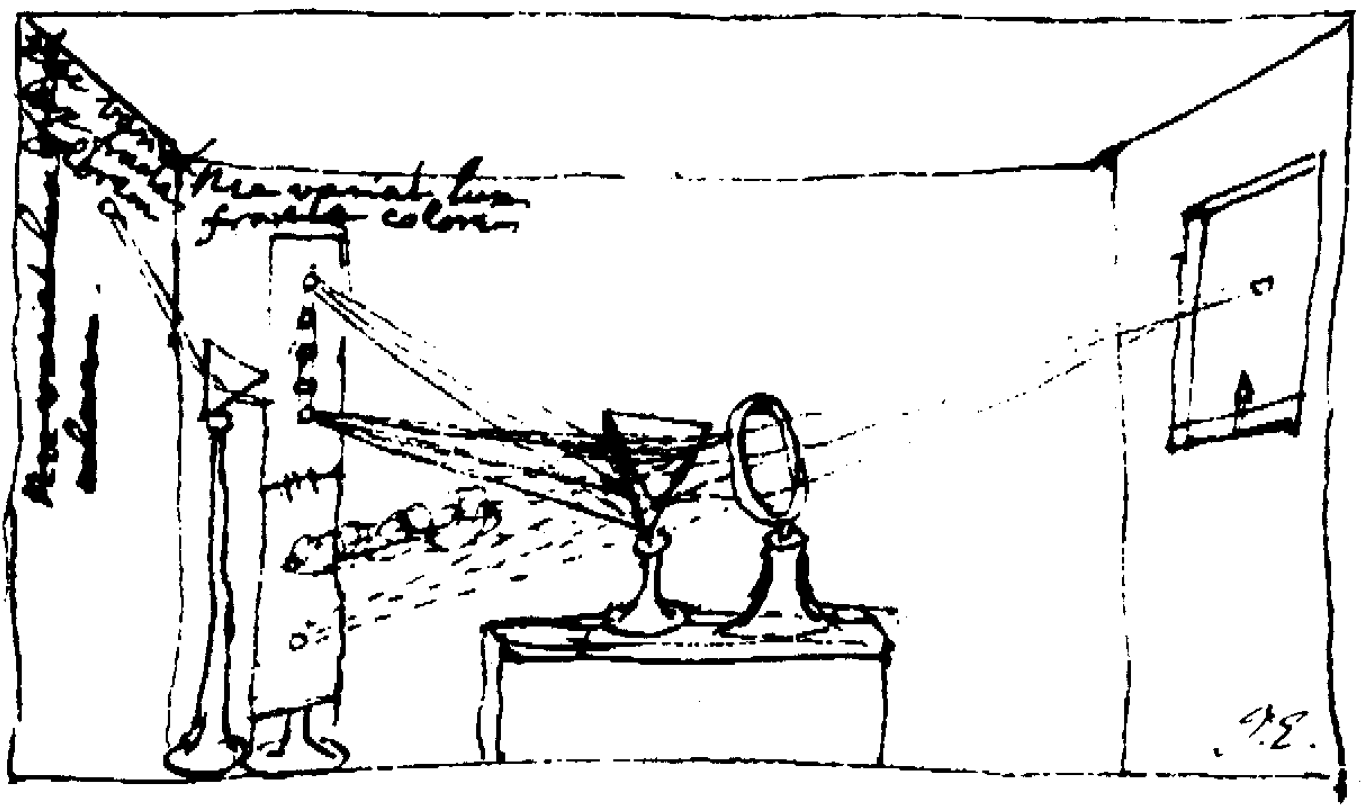
\includegraphics[width=0.9\textwidth,height=\textheight]{wp-content/uploads/2012/02/newton.png}

}

\caption{\label{fig-newton}Newton's summary drawing of his experiments
with light. Using a point source of light and a prism, Newton separated
sunlight into its fundamental components. By reconverging the rays, he
also showed that the decomposition is reversible.}

\end{figure}%

From this experiment, Newton concluded that the pass through the first
prism had separated the daylight into its fundamental components. No
further change was observed when the ray passed through a second prism.

At the bottom of the sketch Newton illustrated that the decomposition is
reversible: passing light through the prism does not destroy the
character of the light. To show this Newton converged the rays following
their passage through the prism to form a new image; he found that the
color of the image same is the same as that of the source. Newton
concluded that:

\begin{quote}
\emph{``Light being transmitted through the parallel surfaces of two
prisms \ldots{} if it suffered any change by the refraction by one
surface, it lost that impression by the contrary refraction of the other
surface.''(Newton (1984))}
\end{quote}

From the second experiment, he concluded that passage through the prism
had not destroyed, but merely revealed, the character of the light.

We now know that Newton succeeded in decomposing the sunlight into its
\emph{spectral} components, each with its own characteristic wavelength.
The prism separates the rays because the prism bends each wavelength of
light by a different amount. (See the section on Snell's law in
Chapter~\ref{sec-image-formation}). When we see the spectral components
separately, they each have a different color appearance. Light with
relatively long wavelengths appears red when viewed against a dark
background. Light with relatively short wavelengths appears blue when
viewed against a dark background. Shorter wavelengths of light are
refracted more strongly than longer wavelengths. A spectral light, with
energy only at a single wavelength, is also called a \emph{monochromatic
light}.

\begin{figure}

\centering{

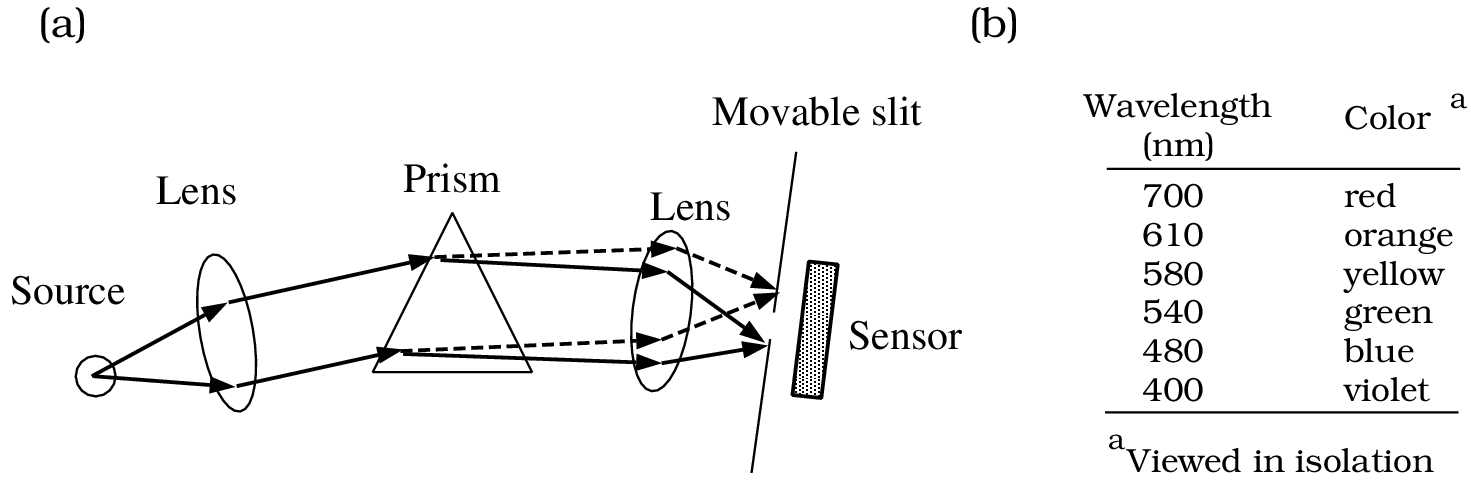
\includegraphics[width=0.8\textwidth,height=\textheight]{wp-content/uploads/2012/02/spectroradiometer.png}

}

\caption{\label{fig-spectroradiometer}A spectroradiometer is used to
measure the spectral power distribution of light. (a) A schematic design
of a spectroradiometer includes a means for separating the input light
into its different wavelengths and a detector for measuring the energy
at each of the separate wavelengths. (b) The color names associated with
the appearance of lights at a variety of wavelengths are shown (After
Wyszecki and Stiles (1982)).}

\end{figure}%

Newton's apparatus suggests a simple device we might build to measure
the amount of power a light has in each of the different wavelength
bands. As illustrated on the top of Figure~\ref{fig-spectroradiometer},
by proper use of lenses and prisms, we can form a focused image of the
spectral components in an image plane with a movable slit placed in
front of a photodetecting sensor. To measure the energy at different
wavelengths, we move the slit passing only some of the spectral
components at each position, and thus we measure the energy of the
source at different wavelengths of light. In the visible region, the
wavelength of light is on the order of a few hundred billionths of a
meter, or \emph{nanometers} (nm).

The \emph{spectral power distribution} of a light is the function that
defines the power (Watts = Joules/sec) in the light in each wavelength
band. In the modern theory of physics, the wavelength of light can be
thought of in two different ways. We describe the light as if it were a
continuous wave as it passes through a medium. When the light exchanges
energy with some material, say by giving up its energy to be absorbed,
we describe the light as if it were a discrete object called a
\emph{photon} or \emph{quantum} of light. The amount of energy given up
by the photon is predicted by the wavelength of the light.

\begin{figure}

\centering{

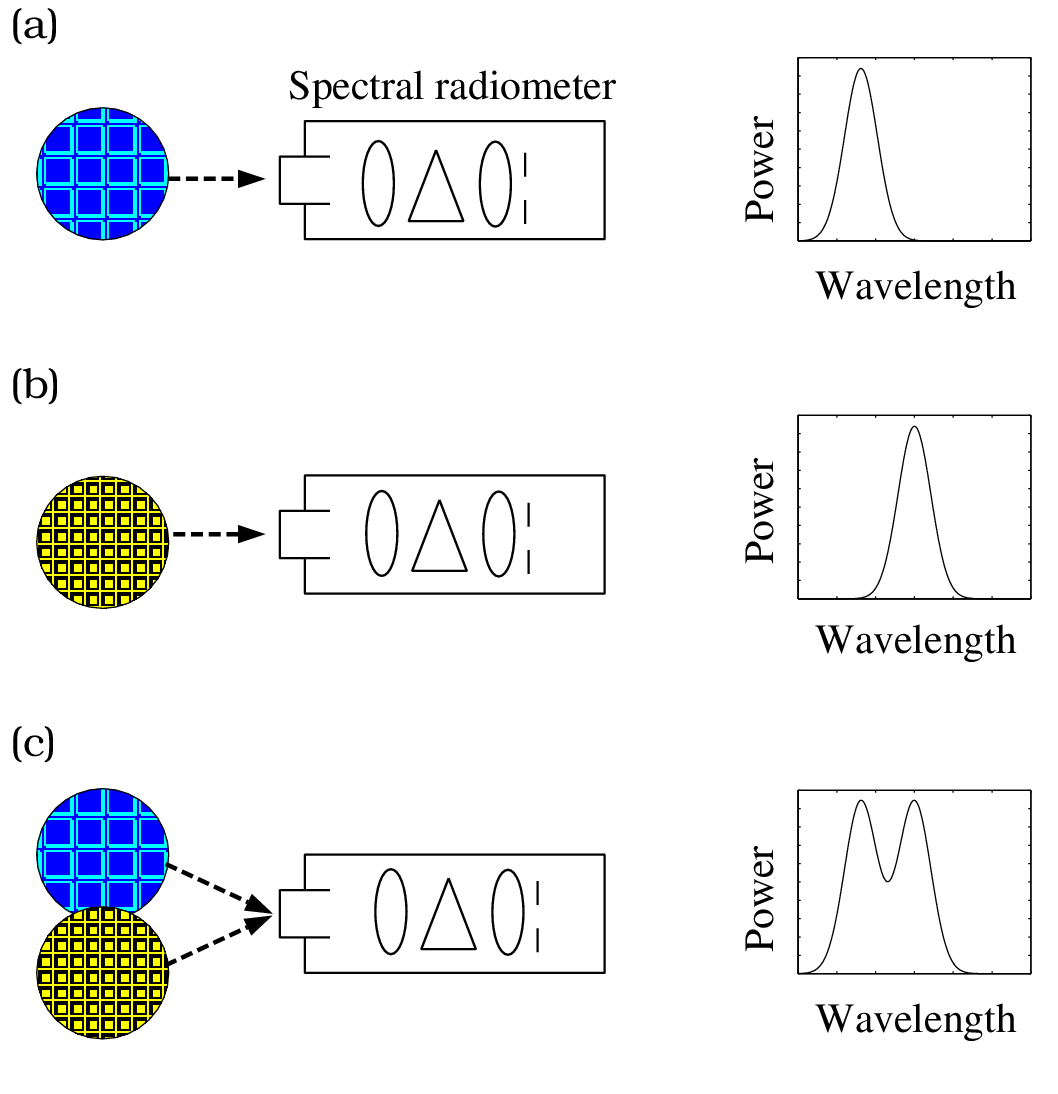
\includegraphics[width=0.6\textwidth,height=\textheight]{wp-content/uploads/2012/02/ill.superposition.png}

}

\caption{\label{fig-superposition}Principle of Superposition. The
measurement of light spectral power distributions satisfies the
principle of superposition. The spectral power distributions of two
lights measured separately are shown in (a) and (b) and together in (c).
The spectral power distribution of the mixture is the sum of the
individual measurements, thus demonstrating that superposition holds
true.}

\end{figure}%

The experimental aspect of light measurement that makes it useful and
predictable is that the measurement satisfies the principle of
superposition. We can demonstrate the superposition of light measurement
as follows. First, measure the spectral power distributions of two
lights separately. Then, mix the two lights together and measure again.
The spectral power distribution of the mixture will be the sum of the
first two spectral power distributions. This property of light mixture
is illustrated in Figure~\ref{fig-superposition}. Superposition is a
crucial property of light measurement because it implies that we can
measure the energy of a light at each wavelength separately, and then
combine the individual measurements to predict spectral power
distribution when the spectral components are mixed together.

Suppose we wish to measure the spectral power distribution of a light
source. How many wavelengths should we measure? Or, equivalently, how
finely do we have to sample along the wavelength dimension? The answer
to this question is important for both practical and theoretical reasons
because the number of samples can be quite large. For example, to sample
the visible spectrum from 400 nm to 700 nm in 1 nm steps, we need about
300 measurements. To sample in 10 nm steps, we need about 30
measurements.

The answer to this sampling question depends on the same set of issues
as the sampling questions we addressed in
Chapter~\ref{sec-photoreceptor-mosaic} on the spatial sampling of the
retinal image by the photoreceptor mosaics. If the energy in the light
varies rapidly as a function of wavelength, then we may have to sample
quite finely to measure accurately; if the functions vary slowly, then
only a few measurements are necessary. Also, the precision of the
representation requires that we know how sensitive the photopigments in
the are to rapid changes in the energy as a function of wavelength.

\begin{figure}

\centering{

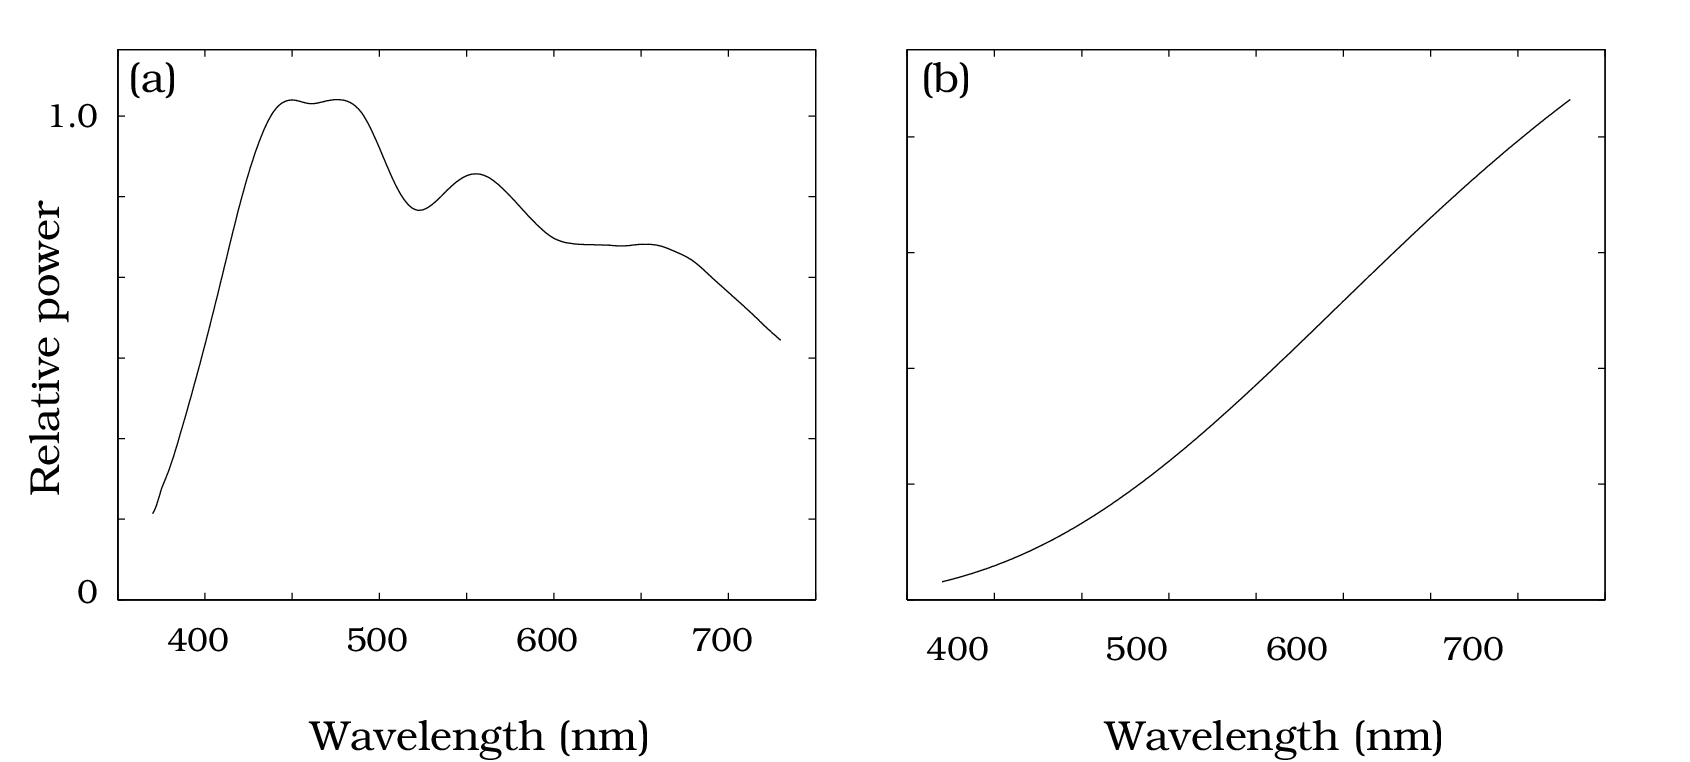
\includegraphics[width=0.6\textwidth,height=\textheight]{wp-content/uploads/2012/02/spectra1.png}

}

\caption{\label{fig-spectra1}The spectral power distribution of two
important light sources are shown: blue skylight (a) and the yellow disk
of the sun (b).}

\end{figure}%

It is difficult to make accurate generalizations about how spectral
power distributions vary as a function of wavelength, but it is believed
widely that for practical purposes we can approximate spectral power
distributions using smooth, regular functions as shown in
Figure~\ref{fig-spectra1}. Also, it is known that the photopigments
integrate broadly across the wavelength spectrum. Consequently,
international standards organizations suggest making measurements every
5 nm to achieve an excellent representation of the signal. Practical
measurements often rely on measurements spaced every 10 or 20 nm. We
will consider this issue much more completely when we review color
appearance, in Chapter~\ref{sec-color}.

\section{Scotopic Wavelength
Encoding}\label{sec-scotopic-wavelength-encoding}

What information do we encode about the spectral power distribution when
rods initiate vision, under \emph{scotopic} conditions? We can answer
this question by an experiment designed to measure how well people can
discriminate different spectral power distributions. In the
\emph{scotopic matching} experiment, we present an observer with two
lights, side by side in a \emph{bipartite} field. One side of the field
contains the \emph{test} light; it may have any spectral power
distribution whatsoever. The second side of the field contains the
\emph{primary} light; it has a fixed relative spectral power
distribution and can vary only by an overall intensity factor. The
observer's task in the \emph{scotopic matching experiment} is to adjust
the primary light intensity so that the primary light appears
indistinguishable from the test light. The observer can adjust only the
intensity of the primary light, so when the match is achieved the
spectral power distributions of the test and primary lights that match
are still different.

Under scotopic conditions, observers can adjust the primary intensity so
that the primary matches any test light. Since subjects can always make
this match, we have a simple answer to our question: The rods encode
nothing about the relative spectral density of a light. An observer can
adjust the intensity of a primary light to match the appearance of a
test light with any spectral power distribution. The relative spectral
power distribution is immaterial, all that matters is the relative
intensities of the two lights.

\subsection{Matching: Homogeneity and
superposition}\label{matching-homogeneity-and-superposition}

We can learn more about scotopic wavelength encoding by studying the
quantitative properties of the matching experiment. To characterize the
matching experiment completely, we must be able to predict how a subject
will adjust the primary intensity to match any test light. We treat the
experiment as a transformation by identifying the spectral power
distribution of the test light as the input and the intensity of the
primary light as the output. A quantitative description of the
experiment tells us how to map the input to the output.

Naturally, we first ask whether we can characterize the matching
experiment transformation using linear systems methods. Denote the
spectral power distribution of the test and primary lights using the
vectors \(\mathbf{t}\) and \(\mathbf{p}\) respectively. The
\(n_{\lambda}\) entries of these vectors describe the power at each of
the \(n_{\lambda}\) sample wavelengths. To test linearity, we evaluate
whether the scotopic matching experiment satisfies the linear systems
properties of homogeneity and superposition. We can evaluate these
properties from the following experimental tests:

\begin{itemize}
\tightlist
\item
  (Homogeneity) If \(\mathbf{t}\) matches \(e \mathbf{p}\), will
  \(a \mathbf{t}\) match \(a (e \mathbf{p})\)?
\item
  (Superposition) If \(\mathbf{t}\) matches \(e \mathbf{p}'\), and
  \({\mathbf{t}'}\) matches \({e'} \mathbf{p}'\), will
  \(\mathbf{t} + \mathbf{t}'\) match
  \(( e \mathbf{p} ) + ( e' \mathbf{p} )\)?
\end{itemize}

An hypothetical test of homogeneity is shown in
Figure~\ref{fig-scotopic}. The separate panels show the intensity of the
test light on the horizontal axis and the intensity of the matching
primary light on the vertical axis. Each panel plots the results using
spectral test lights at a series of wavelengths and a 510 nm primary
light. In the scotopic matching experiment the data will fall on a
straight line, consistent with the prediction from homogeneity. The
slope of the line defines the relative scotopic sensitivity to the test
and the primary lights. For example, in panel (c) the hypothetical
results from an experiment with a 580 nm test light are shown. The slope
of the line shows that we need \(8.3\) units of energy at 580 nm to have
the same effect as one unit of energy at 510 nm. Hence, the light at 510
nm is \(8.3\) times more effective, per unit energy, than the light at
580 nm.

\begin{figure}

\centering{

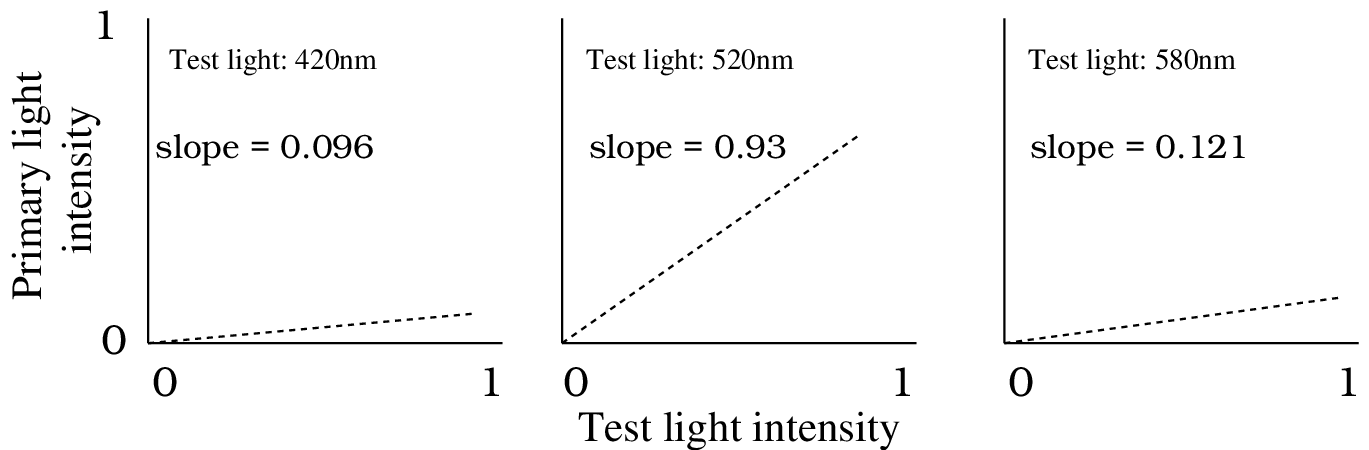
\includegraphics[width=0.8\textwidth,height=\textheight]{wp-content/uploads/2012/02/scotopic.png}

}

\caption{\label{fig-scotopic}Hypothetical scotopic matching experiment.
The horizontal scale measures the intensity of a monochromatic test
light and the vertical scale measures the intensity a matching 510 nm
primary light. Since the scotopic matching experiment satisfies
homogeneity, the data will fall along a straight line. The slope of the
line defines the relative scotopic sensitivity to each test wavelength.}

\end{figure}%

Because the scotopic matching experiment is linear, there must be a
system matrix, \(\mathbf{R}\) that maps the input (\(\mathbf{t}\), the
test spectral power distribution), to the output (\(e\), the primary
light intensity). The system matrix, call it \(\mathbf{R}\), must have
one row and \(n_{\lambda}\) columns. The test light, system matrix, and
primary intensity are related by the product,
\(e = \mathbf{R} \mathbf{t}\).

\begin{figure}

\centering{

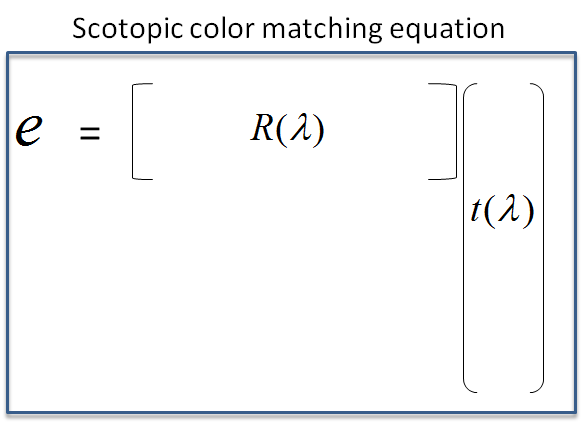
\includegraphics[width=0.5\textwidth,height=\textheight]{wp-content/uploads/2012/02/Scotopic-Tableau.png}

}

\caption{\label{fig-scotopic-tableau}Matrix tableau of the scotopic
matching experiment. The primary light intensity, e, equals the product
of the \(1 \times n_{\lambda}\) scotopic matching system matrix and the
\(n_{\lambda} \times 1\) vector representing the test light spectral
power distribution.}

\end{figure}%

We can relate the measurements in the scotopic matching experiment to
the entries of the system matrix as follows. Write the matrix product
\(\mathbf{R} \mathbf{t}\) as a summation over the sample wavelengths,

\begin{equation}\phantomsection\label{eq-scotopic-sum}{
e = \sum_{i=1}^{i=n_{\lambda}} R_{i} \mathbf{t}_{i}
}\end{equation}

Suppose we use a monochromatic test light of unit intensity, that is, an
input \(\mathbf{t}\) that has only a single non-zero wavelength,
\((0,0,...,0,1,0,...0)^{T}\). Then Equation~\ref{eq-scotopic-sum}
becomes simply \(e = R_{i} \mathbf{t}_{i}\). This shows that the slope
of the line relating the monochromatic test intensity,
\(\mathbf{t}_{i}\), to the primary intensity, \(e\), is the system
matrix entry, \(R_{i}\). Hence, we can estimate the system matrix from
the slopes of the experimental lines we measure in the test of
homogeneity shown in Figure~\ref{fig-scotopic}.

\begin{figure}

\centering{

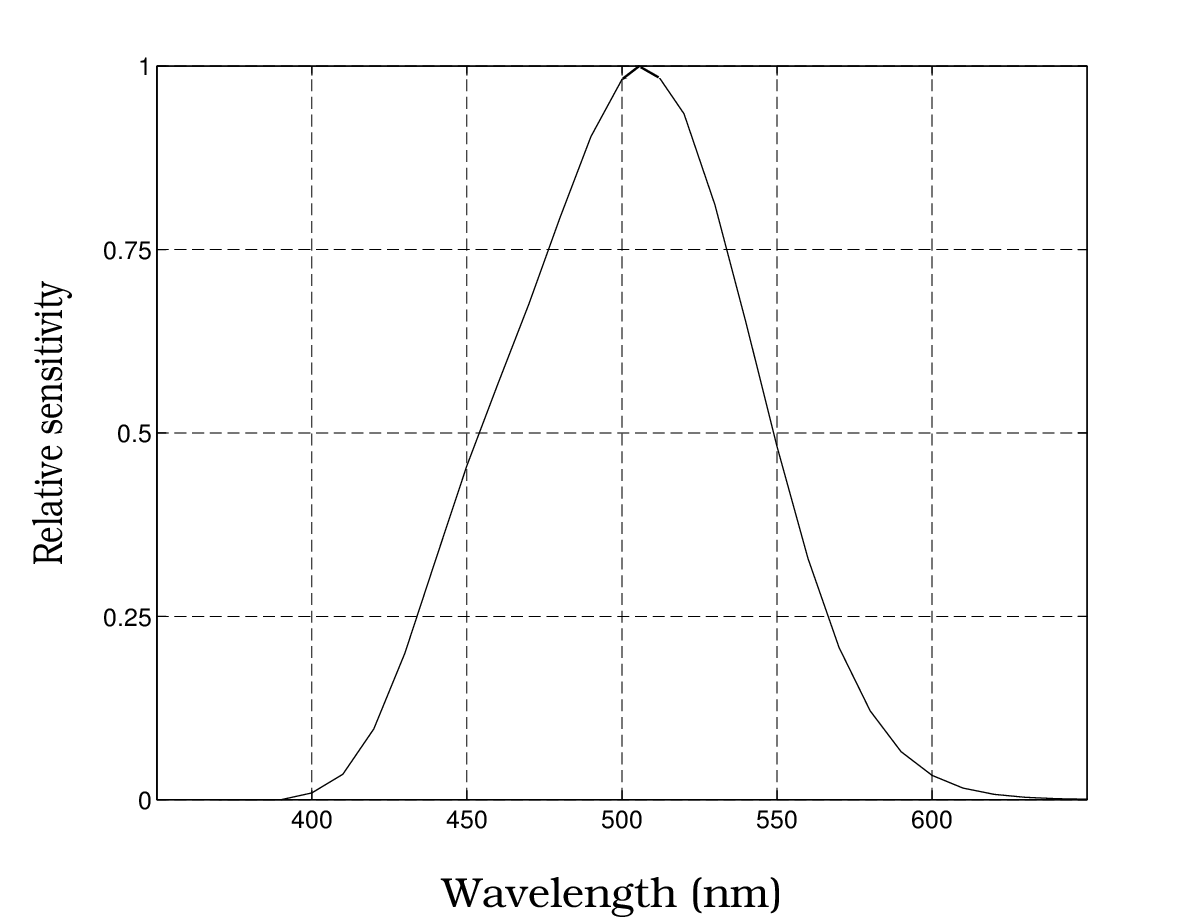
\includegraphics[width=0.6\textwidth,height=\textheight]{wp-content/uploads/2012/02/scot.sens_.png}

}

\caption{\label{fig-scotopic-sens}The scotopic spectral sensitivity
function defines the human wavelength sensitivity under scotopic viewing
conditions. The curve is a plot of the entries of the scotopic system
matrix.}

\end{figure}%

Figure~\ref{fig-scotopic-sens} is a graphical method of representing the
system matrix of the scotopic matching experiment. The curve shows the
entries of \(\mathbf{R}\) as a function of wavelength, interpolated from
experimental measurements at many sample wavelengths. The curve is
called the \emph{scotopic sensitivity function}.

Once we measure the system matrix, \(\mathbf{R}\), we can predict
whether any pair of lights will match under scotopic conditions. The
matrix tableau shows how we use the system matrix to predict the
intensity of a primary light needed to match a test light. Suppose we
have two test lights, \(\mathbf{t}\) and \(\mathbf{t} '\). Two lights
will match when they are matched by the same intensity of the primary
light. So, these two lights will match when
\(\mathbf{R} \mathbf{t} = \mathbf{R} \mathbf{t} '\).

\subsection{Uniqueness}\label{uniqueness}

The hypothetical experiment illustrated in
Figure~\ref{fig-scotopic-tableau} assumed a 510 nm primary light.
Suppose that we perform the scotopic matching experiment using a
different primary light. How will this effect the system matrix,
\(\mathbf{R}\)?

We can answer this question by a thought experiment. Call the second
primary light \(\mathbf{p}'\). We can set a match between the new
primary light, \(\mathbf{p}'\), and the first primary light
\(\mathbf{p}\). We will find that there is some scalar, \(k\), such that
\(k \mathbf{p}'\) matches \(\mathbf{p}\), and we expect that whenever
\(a \mathbf{p}\) matches a test light, \(\mathbf{t}\), then
\(a (k \mathbf{p}')\) will match \(\mathbf{t}\). In particular, since
\(R_{i} \mathbf{p}\) matches the \(i^{th}\) monochromatic test light, we
expect that \(R_{i} k \mathbf{p}'\) will match the \(i^{th}\)
monochromatic test light as well. It follows that the entries of the new
system matrix will be \(k R_{i}\), equal to the original except for a
constant scale factor, \(k\). Hence, the new system matrix will be
\(k \mathbf{R}\), and we say that the estimate of \(\mathbf{R}\) is
unique up to an unknown scale factor.

\subsection{The Biological Basis of Scotopic
Matching}\label{the-biological-basis-of-scotopic-matching}

Color Plate 1 is a photograph of the photopigment contained in the rod
outer segments. In part (a) of the figure the photopigment is
photographed in the eye of an alligator. Because the back of the
alligator's eye contains a white reflective surface, called the
\emph{tapetum}, it is possible to see the color of the rod photopigment.
Cats too have a white tapetum, which is why cats eyes appear to glow so
brightly when they catch the beam of a car's headlights. The alligator
shown in the picture had been kept in a dark closet for 24 hours so that
the photopigment would be fully regenerated and easy to photograph. The
closet was opened briefly, a flash picture taken, and then I suppose the
door was shut again. Whew. \nocite{RushtonAlligatorSciAm}

\begin{figure}[H]

{\centering 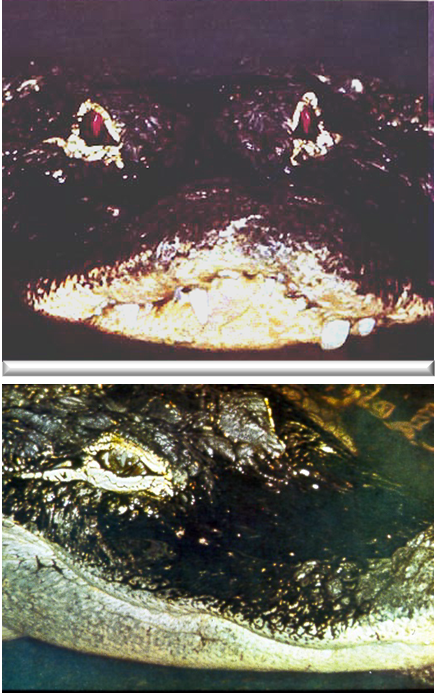
\includegraphics[width=0.6\textwidth,height=\textheight]{wp-content/uploads/2012/02/Alligator.png}

}

\caption{\textbf{Color Plate 1.} The scotopic matching experiment is
remarkable in its simplicity. We can understand the biological basis of
the experimental matches by studying the properties of the rod
photopigment, rhodopsin.}

\end{figure}%

Rod photopigment is present in much higher density than any of the cone
photopigments. Thus, researchers have been able to isolate and extract
the rod photopigment for fifty years, whereas the cone photopigments
have only become available recently through the methods of genetic
engineering (Merbs and Nathans (1992)). Characteristically, when the rod
photopigment is exposed to light, it undergoes a series of rapid changes
in chemical state (Hubbard and Wald (1951); Wald and Brown (1958); Wald
(1968)). Whenever a quantum of light is absorbed by the rhodopsin
photopigment, it undergoes a specific sequence of events resulting in
the decomposition of the rhodopsin molecule into opsin and vitamin A.
Color Plate 1 (b) shows the same alligator after its eye has been
exposed to light. The rhodopsin is been broken into two parts and the
resulting products are clear, rather than purple. In this state, the
white tapetum of the eye is evident. It is the wavelength selectivity of
the rhodopsin photopigment that provides the biological basis of
scotopic matching. The relationship between the behavioral experiment
and the properties of the rod photopigment is based on an important
property called \emph{univariance}.

W. Rushton emphasized that when a photopigment molecule absorbs light,
the effect upon the photopigment is the same no matter what the
wavelength of the absorbed light might be. Thus, even though quanta at
400 nm possess more energy than quanta at 700 nm, the sequence of
rhodopsin reactions to absorption of a 400 nm quantum is the same as the
sequence of reactions to a 700 nm quantum. Rushton used the word
\emph{univariance} for this principle to remind us that a single
photopigment makes only a single-variable response to the incoming
light. The photopigment maps all spectral lights into a single-variable
output, the \emph{rate of absorptions}. The response of a single
photopigment does not encode any information about the relative spectral
composition of the light. This explains why we cannot discriminate
between lights with different spectral power distributions under
scotopic viewing conditions (Rushton (1965); Naka and Rushton (1966)).

\begin{figure}

\centering{

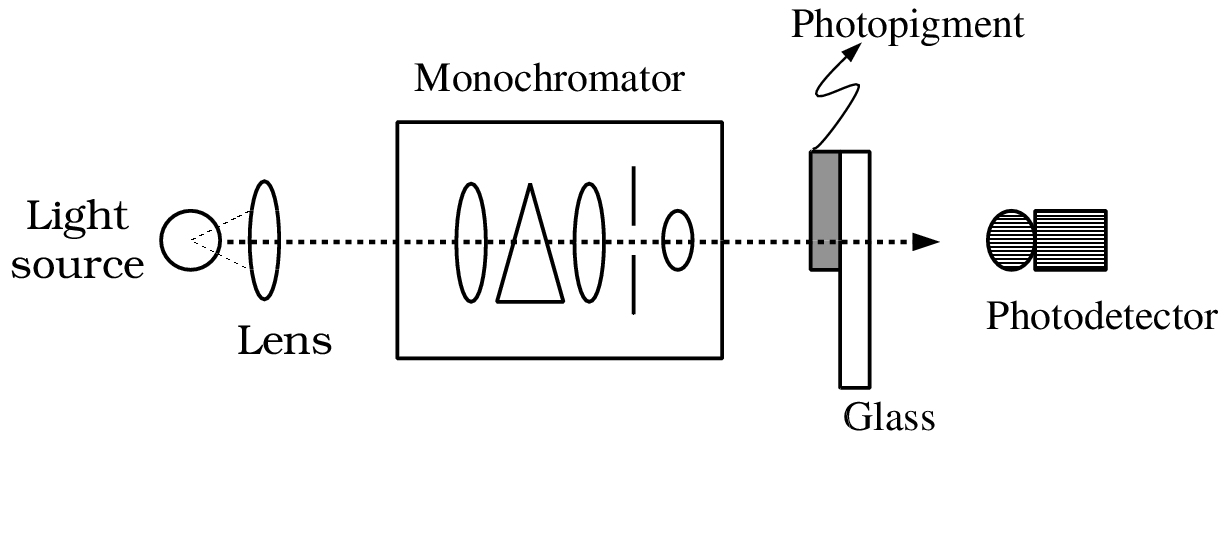
\includegraphics[width=0.7\textwidth,height=\textheight]{wp-content/uploads/2012/02/self.screening1.png}

}

\caption{\label{fig-self-screening}An apparatus to measure the spectral
absorption of a photopigment. Using the monochromator, one can select
light at one wavelength from the light source. To estimate the fraction
of photons absorbed by the photopigment at that wavelength, we divide
the number of photons detected through the glass and photopigment by the
number detected after passing through the glass alone.}

\end{figure}%

Univariance does not mean, however, that the photopigment responds
equally well to all spectral lights. The photopigment is much more
likely to absorb some wavelengths of light than others. Univariance
asserts that once absorbed, however, all quanta have same visual effect.

We can measure the probability of absorption using the experimental
apparatus shown in Figure~\ref{fig-self-screening}. We place a thin
layer of photopigment on a clear plate of glass. We create a
monochromatic light by passing the light from an ordinary source through
a \emph{monochromator}. The monochromator can be constructed using
prisms or diffraction gratings to separate the incident light into its
separate wavelengths, much as in Newton's original experiments. We
measure the amount of monochromatic light passed through the
photopigment and the glass plate by means of a photodetector at the rear
of the apparatus. We then move the glass plate upwards, to remove the
photopigment from the light path, and measure again. The difference in
the photodetector signal measured in these two conditions is
proportional to the amount of light absorbed by the photopigment.

\begin{figure}

\centering{

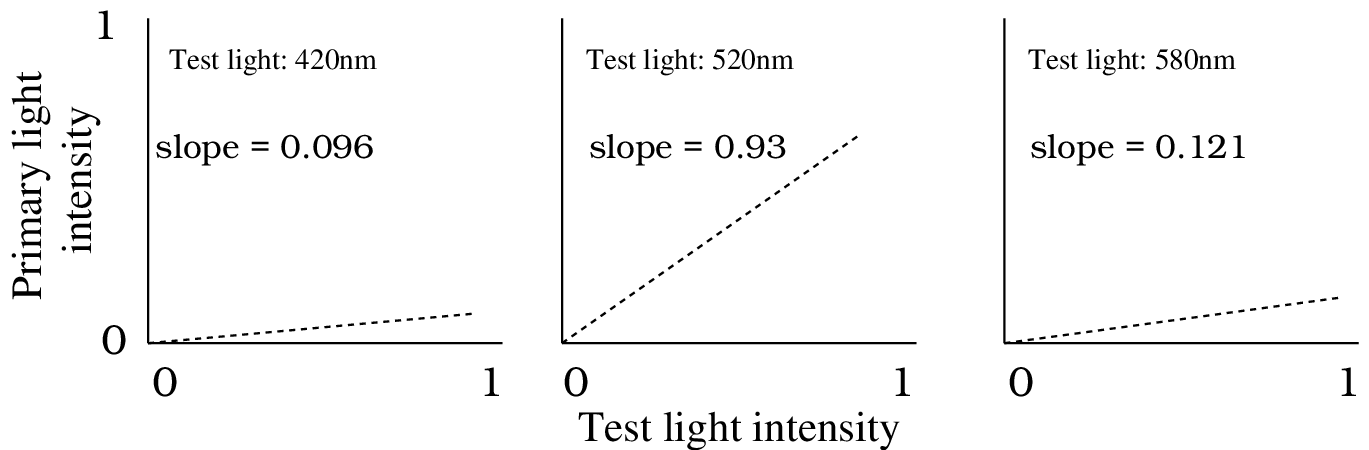
\includegraphics[width=0.7\textwidth,height=\textheight]{wp-content/uploads/2012/02/scotopic1.png}

}

\caption{\label{fig-scotopic1}Rhodopsin absorptions at different
wavelengths. The number of absorptions in a thin layer of photopigment
are proportional to the intensity of the input light and thus satisfy
the principle of homogeneity. The slope of the linear relationship
between the light intensity and the number of absorptions describes the
fraction of photon absorptions. The slope varies with the wavelength of
the test light, thus defining the photopigment wavelength sensitivity.}

\end{figure}%

If only a thin layer of photopigment is present, the experimental
measurements of the absorptions will satisfy homogeneity and
superposition. To test homogeneity, we increase the intensity of the
test light. We will find that the number of absorptions will increase
proportionately over a significant range. To test superposition, we
measure the photopigment absorptions to a test light \(\mathbf{t}\) to
be \(a\), and the number of absorptions to a second light
\(\mathbf{t}'\) to be \(a'\). When we superimpose the two input lights,
we will measure \(a + a'\) absorptions. Since the measurement process is
linear, we can estimate the system matrix of this absorption process,
\(\mathbf{A}\), just as we measured the system matrix of the scotopic
matching experiment, \(\mathbf{R}\).

\begin{figure}

\centering{

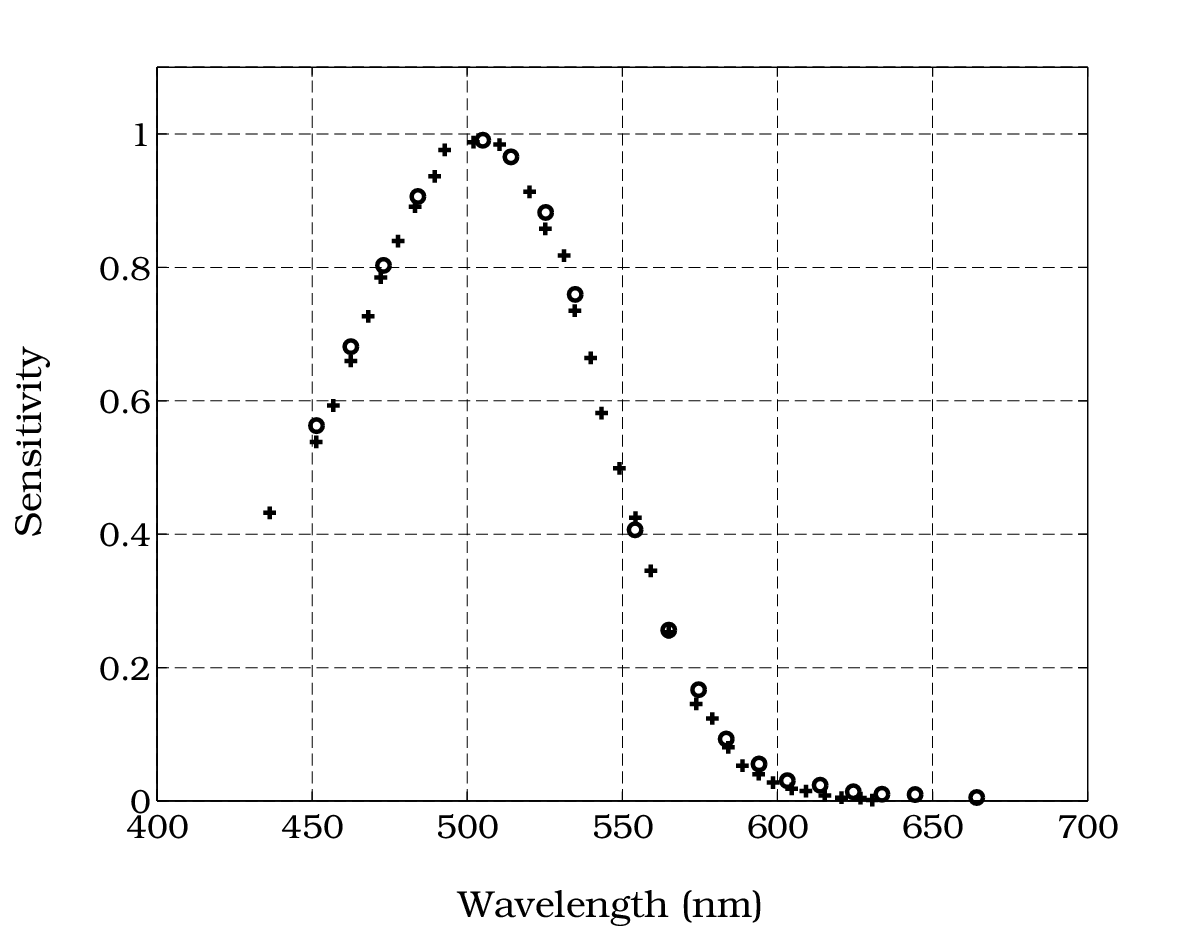
\includegraphics[width=0.6\textwidth,height=\textheight]{wp-content/uploads/2012/02/rhodopsin.sens_.png}

}

\caption{\label{fig-rhodopsin-sens}Comparisons of scotopic matching and
rhodopsin wavelength sensitivity. The filled circles show human
rhodopsin absorption measured as in Figure~\ref{fig-scotopic1}. The open
circles show human scotopic sensitivity, corrected for light loss at the
lens and optical media. (Source: Wald and Brown (1958))}

\end{figure}%

We can predict the matches in the scotopic matching experiment from the
absorptions of the rhodopsin photopigment. A test and primary light
match in the scotopic matching experiment when the two lights create the
same number of absorptions in the rhodopsin photopigment. We can
demonstrate this by comparing the system matrices of the scotopic
matching experiment and the rhodopsin absorption experiment. After we
correct for the effects of the wavelength sensitive elements of the eye,
mainly the lens, we can plot the system matrices of the scotopic
matching experiment \(\mathbf{R}\), and the rhodopsin absorption
experiment, \(\mathbf{A}\), on the same graph. Wald and Brown (1958)
made this comparison in the graph shown in
Figure~\ref{fig-rhodopsin-sens}. The filled circles in the graph plot
the measurements of the system matrix from the rhodopsin absorption
experiment, \(\mathbf{A}\). The completely open circles plot estimates
of the entries of \(\mathbf{R}\) after correcting for the fact that the
lens absorbs a significant amount of light in the short-wavelength part
of the spectrum.

The agreement between the measurements of the rhodopsin photopigment and
the scotopic matching experiment confirm a simple model of the
observer's behavior. Under scotopic viewing conditions the observer's
perception of the two halves of the bipartite field depends on a signal
initiated by the rod photopigment absorptions. The two sides of the
field appear identical when the rhodopsin absorption rates on the two
sides of the bipartite field are equal. During the experiment, then, the
observer adjusts the intensity of the matching light to equalize the rod
absorption rates on the two sides of the bipartite field. Since the
absorption of the light is a linear process, the observer's behavior is
linear, too.

The precise quantitative match between the scotopic matches and the rod
photopigment make a very strong connection between performance and
biological encoding of the light. This type of precise quantitative
relationship between behavior and the biological encoding of light
serves as a good standard to use when we consider the relationship
between behavior and biology in other conditions.

\section{Photopic Wavelength
Encoding}\label{photopic-wavelength-encoding}

When the cones initiate vision, under photopic conditions, we do encode
some information about the relative spectral power distribution of the
incident light. Changes in the relative spectral power distributions
result in changes of the color appearance of the light. Several of the
important properties of color appearance can be traced to the way cone
photoreceptors encode the relative spectral power distribution of
light\footnote{Color appearance is not a simple consequence of the
  spectral power distribution of the incident light. We will discuss
  color appearance broadly in Chapter~\ref{sec-color}.}.

\begin{figure}

\centering{

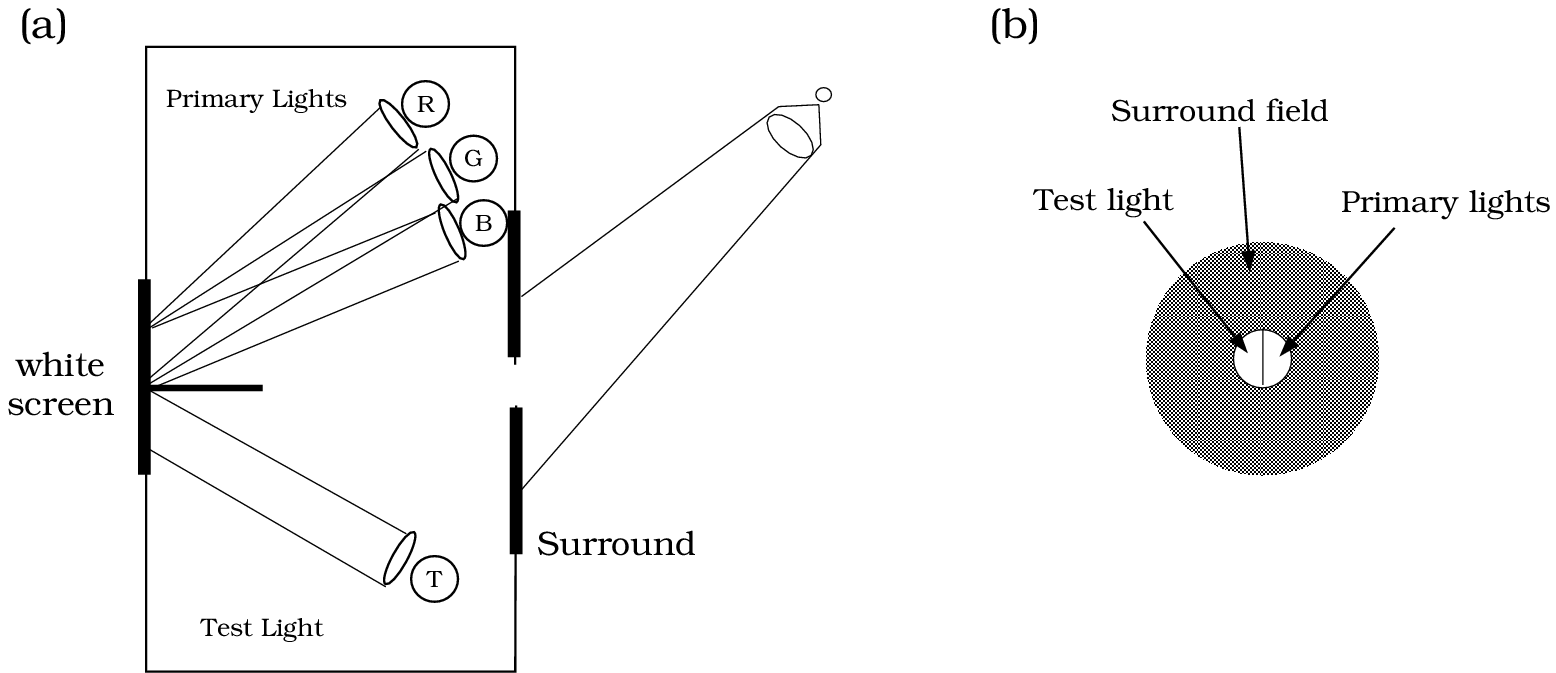
\includegraphics[width=0.6\textwidth,height=\textheight]{wp-content/uploads/2012/02/colorMatching.png}

}

\caption{\label{fig-color-matching}The color-matching experiment. The
observer views a bipartite field and adjusts the intensities of the
three primary lights to match the appearance of the test light. (a) A
side-view of the experimental apparatus. (b) The appearance of the
stimuli to the observer. (After Judd and Wyszecki (1975))}

\end{figure}%

We will relate the human ability to discriminate lights to the
properties of the cones just as we did with the rods. First, we will
review the matching experiments that characterize how well people can
discriminate between lights with spectral power distributions. When we
measure under photopic conditions, the experiment is called the
\emph{color-matching} experiment. The color-matching experiment is the
foundation of color science and of direct significance to many color
applications (see the Appendix). Second, we will relate the properties
of the color-matching experiment to the properties of the cone
photopigments. The analysis of photopic wavelength encoding parallels
the analysis of scotopic wavelength encoding. The main differences are
that (a) we must keep track of the photopigment absorptions in three
cone photopigments rather than the single rod photopigment, and (b)
until quite recently the cone photopigments were not present in
sufficient quantity to define their properties with any certainty (Merbs
and Nathans (1992)). Hence, the problem of relating color-matching and
the cone photopigments was solved using other indirect biological
measurements. We can learn a great deal from studying the logic of these
methods.

Figure~\ref{fig-color-matching} shows a simple apparatus that can be
used to perform the color-matching experiment. The observer views a
bipartite visual field with the test light on one side. The test light
may have any spectral power distribution. The second half of the
bipartite field contains a mixture of \emph{three} primary lights.
Throughout the experiment, the relative spectral power distribution of
each primary light is constant; only the absolute level of the primary
lights can be adjusted. The observer's task is to adjust the intensities
of the three primary lights so that the two sides of the bipartite field
appear identical.

\begin{figure}

\centering{

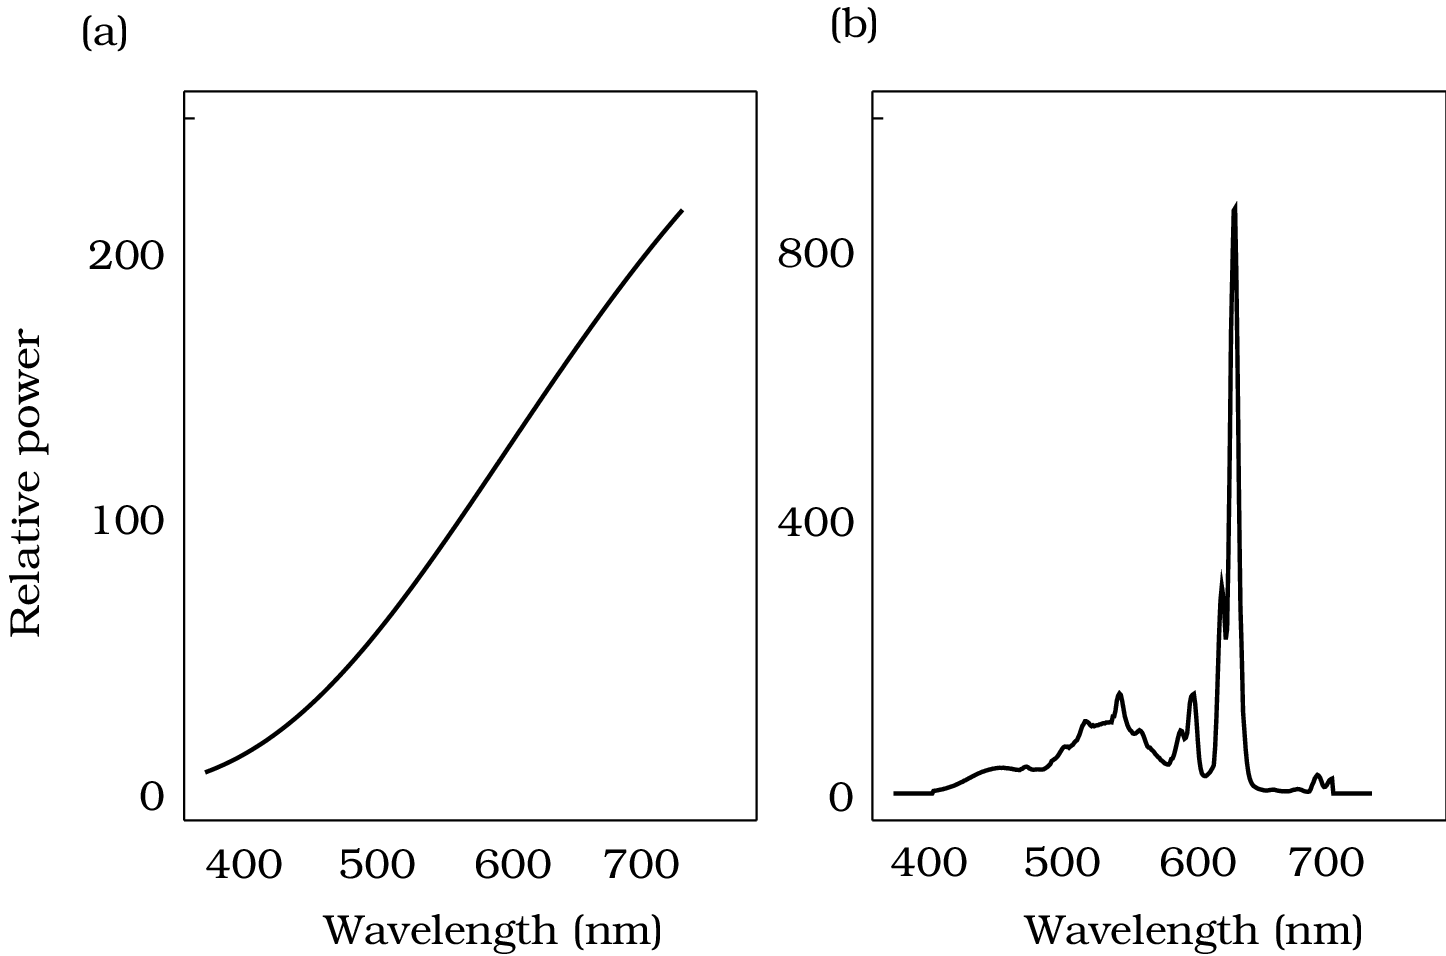
\includegraphics[width=0.6\textwidth,height=\textheight]{wp-content/uploads/2012/02/tvMetamers.png}

}

\caption{\label{fig-tv-metamers}Metameric lights. Two lights with these
spectral power distributions appear identical to most observers and are
called metamers. The curve in part (a) is an approximation to the
spectral power distribution of the sun. The curve in part (b) is the
spectral power distribution of a light emitted from a conventional
television monitor whose three phosphor intensities were set to match
the light in (a) in appearance.}

\end{figure}%

When the observer has completed setting an appearance match, the lights
on the two sides of the bipartite field are not physically the same. The
test light can have any spectral power distribution, while the mixture
of primaries can only have a limited number of spectral power
distributions determined by the possible weighted sums of the three
primary light spectral power distributions. Lights that are photopic
appearance matches, but that are physically different, are called
\emph{metamers}. Figure~\ref{fig-tv-metamers} contains a pair of
spectral power distributions that match visually but differ physically,
i.e.~a pair of metamers.

The metamers in Figure~\ref{fig-tv-metamers} illustrate that even under
photopic viewing conditions we fail to discriminate between very
different spectral power distributions. To understand the behavioral
aspects of photopic wavelength encoding, we must try to predict which
spectral power distributions we can discriminate. The first question we
ask is whether we can predict performance in the photopic color-matching
experiment using linear systems methods.

\begin{figure}

\centering{

\includegraphics[width=0.8\textwidth,height=\textheight]{wp-content/uploads/2012/02/phot.superposition.png}

}

\caption{\label{fig-phot-superposition}The color-matching experiment
satisfies the principle of superposition. In parts (a) and (b) test
lights are matched by a mixture of three primary lights. In part (c) the
sum of the test lights is matched by the additive mixture of the
primaries, demonstrating superposition.}

\end{figure}%

We can define the experimental measurements in the color-matching
experiment in direct analogy with the definitions we used in the
scotopic matching experiment. The input variable in the color-matching
experiment is the light \(\mathbf{t}\), just as in scotopic matching. In
the color-matching experiment, however, the subject's responses consist
of three numbers, not just one. So, we record the responses using a
three-dimensional vector, \(\mathbf{e}\). The entries of \(\mathbf{e}\)
are the intensities of the three primary lights
\(( e{1} , e{2} , e{3} )\). To test superposition in the color-matching
experiment we follow the logic illustrated in
Figure~\ref{fig-phot-superposition}. We obtain a match to a
\(\mathbf{t}\) by adjusting the primary intensities to the levels in
\(\mathbf{e}\). We then obtain a match to \(\mathbf{t} '\) by adjusting
the three primary intensities to \(\mathbf{e} '\). We test additivity by
verifying that the match to \(\mathbf{t} + \mathbf{t} '\); is
\(\mathbf{e} + { \mathbf{e} '}\). Photopic color-matching satisfies
homogeneity and superposition. We honor the person who first understood
the importance of superposition in color-matching by calling this
empirical property \emph{Grassmann's additivity law}.

\begin{figure}[H]

{\centering \includegraphics[width=0.8\textwidth,height=\textheight]{wp-content/uploads/2012/02/photopic.png}

}

\caption{Matrix tableau of color-matching. The photopic color-matching
experiment defines a linear mapping from the test light spectral power
distribution to the intensity of the three primary lights. The rows of
the system matrix are called the color-matching functions. These
functions can be estimated by setting matches to many different test
lights and solving a set of linear equations.}

\end{figure}%

Because the color-matching experiment linearly maps the physical
stimulus \(\mathbf{t}\) to the primary intensities, \(\mathbf{e}\),
there must be a system matrix that maps the input vector \(\mathbf{t}\)
to the output vector \(\mathbf{e}\). The matrix tableau shows the
input-output relationship for the photopic color-matching experiment in
matrix tableau. We will call the \(3 \times n_{\lambda}\) system matrix
\(\mathbf{C}\).

We can estimate the system matrix \(\mathbf{C}\) from the color-matches
in the same way as we estimated the scotopic system matrix: by setting
matches to a collection of monochromatic test lights with unit
intensity. Since the vector representing a monochromatic test light is
zero at each entry but one, the product of the system matrix and the
monochromatic test light vector equals a single column of the system
matrix. Thus, by matching a series of unit intensity monochromatic
lights, we can define each of the columns of the system matrix,
\(\mathbf{C}\).

It is also useful to think of the system matrix in terms of its rows,
which are called the \emph{color-matching functions}. Each row of the
matrix defines the intensity of a single primary light that was set to
match the monochromatic test lights. We will relate the rows of the
photopic system matrix to the properties of the cone photopigments just
as we related the single row of the scotopic system matrix to the
rhodopsin photopigment. However, to make the connection between the cone
photopigments and the color-matching functions will require a little
more work.

\subsection{Measurements of the Color-Matching
Functions}\label{measurements-of-the-color-matching-functions}

Two important caveats arise when we measure the color-matching
functions. These are only a minor theoretical nuisance, but they have
important implications for the laboratory experiment and for practical
applications.

The first issue concerns the selection primary lights. We should chose
lights that are visually \emph{independent}: that is, no additive
mixture of two of the primary lights should be a visual match to the
third primary. This is an obvious but important constraint: it would be
unreasonable to choose the second primary light that looked the same as
the first except for an intensity scale factor. This choice would be
foolish since we could always replace the second light by an
intensity-scaled version of the first primary light, adding nothing to
the range of visual matches we can obtain. Similarly, a primary that can
be matched by a mixture of the first two adds nothing. We must choose
our primary lights so that they are independent of one another.

Even among collections of primary lights that are independent, some are
more convenient than others. Empirically, it turns out that no matter
which primary lights we choose, there will always be some test lights
that cannot be matched by an additive mixture of the three primaries. To
match these test lights, we must move one or even two of the primary
lights from the matching side of the bipartite field to the test side of
the bipartite field. Thus, ordinarily we obtain a visual matches of the
form \begin{equation}\phantomsection\label{eq-cmatch1}{
\mathbf{t} = e_1 \mathbf{p}_1 + e_2 \mathbf{p}_2 + e_3 \mathbf{p}_3 .
}\end{equation}

Shifting one of the primaries to the other side of the bipartite field
means that our match has the form

\begin{equation}\phantomsection\label{eq-cmatch2}{
\mathbf{t} + e_1 \mathbf{p}_1 = e_2 \mathbf{p}_2 + e_3 \mathbf{p}_3 .
}\end{equation}

To a mathematician, Equation~\ref{eq-cmatch2} is the same as

\begin{equation}\phantomsection\label{eq-cmatch3}{
\mathbf{t} = - e_1 \mathbf{p}_1 + e_2 \mathbf{p}_2 + e_3 \mathbf{p}_3 .
}\end{equation}

Hence, when we encode the intensity of the primary light that has been
shifted to the other side of the test field we denote the match using a
negative intensity value\footnote{Changing the sign of the primary
  intensity is a trivial matter for the theorist. It is a nuisance in
  the laboratory, however, and usually impossible in technological
  applications such as color displays. Thus, the issue of selecting
  primaries to minimize the number of times we must make this adjustment
  is of great practical interest.}.

\begin{figure}

\centering{

\includegraphics[width=0.6\textwidth,height=\textheight]{wp-content/uploads/2012/02/cie.rgb_.png}

}

\caption{\label{fig-cie-rgb}The color-matching functions are the rows of
the color-matching system matrix. The functions measured by Stiles and
Burch (1959) using a 10 deg bipartite field and primary lights at the
wavelengths 645.2 nm, 526.3 nm, and 444.4 nm with unit radiant power are
shown.}

\end{figure}%

Figure~\ref{fig-cie-rgb} plots color-matching functions measured by
Stiles and Burch (1959) using three monochromatic primary lights at
645.2 nm, 525.3 nm and 444.4 nm. Each function describes the intensity
of one of the primary lights used to match various monochromatic test
lights. Notice that the intensity of the red primary, at 645.2 nm nm, is
negative over a region of test light wavelengths, indicating that over
this range of test lights the 645.2 nm primary light was added to the
test field.

The color-matching functions are extremely important in color
technology, such as creating images on color monitors and color
printers. I review the application of these methods to color monitors in
the Appendix.

\subsection{Uniqueness of the Color-Matching
Functions}\label{uniqueness-of-the-color-matching-functions}

Suppose two research groups measure the color-matching functions using
different sets of primary lights. One group measures the color-matching
functions using three primary lights \(\mathbf{p}_{i}\), while the
second group uses a different set of primary lights,
\(\mathbf{p}_{i}'\). How will the two sets of color matching functions
be related?

We can answer this question by the following thought experiment. First,
create a matrix whose columns contain the spectral power distributions
of the first group's primary lights, and call this matrix
\(\mathbf{P}\). The spectral power distribution of a mixture of the
primaries, with primary intensities \(\mathbf{e}\), is the weighted sum
of the columns. We can express this mixture using the matrix product
\(\mathbf{P} \mathbf{e}\). Now, we can use the color-matching functions
to predict when a test light will match the mixture of three primaries.
The test and primaries will match when

\begin{equation}\phantomsection\label{eq-photopic-match}{
\mathbf{C} \mathbf{t} = \mathbf{C} \mathbf{P} \mathbf{e}
}\end{equation}

Suppose the second group of researchers can also established matches to
this test light using their primaries. To describe their measurements,
we create a second matrix whose columns contain the spectral power
distributions of the second group's primary lights, \(\mathbf{P}'\).
Call the primary intensities used to match the test with the second
primaries \(\mathbf{e}'\). Since the light \(\mathbf{P}' \mathbf{e}'\)
is a visual matched to the test light, we know that

\begin{equation}\phantomsection\label{eq-photopic-match2}{
\mathbf{C} \mathbf{t} = \mathbf{C} \mathbf{P}' \mathbf{e}'
}\end{equation}

By combining Equation~\ref{eq-photopic-match} and
Equation~\ref{eq-photopic-match2}, we find that the two vectors of
primary intensities, \(\mathbf{e}\) and \(\mathbf{e}'\), are related by
a linear transformation,

\begin{equation}\phantomsection\label{eq-photopic-transform}{
\mathbf{e} = (\mathbf{C} \mathbf{P} )^{-1}\mathbf{C} \mathbf{P}' \mathbf{e}'
}\end{equation}

With a little more algebra, one can show that the color-matching
functions are related by the following linear transformation:

\begin{equation}\phantomsection\label{eq-photopic-transform2}{
\mathbf{C} = ( \mathbf{C} \mathbf{P}') \mathbf{C}'
}\end{equation}

The \(3 \times 3\) matrix relating the two sets of color-matching
functions, \(\mathbf{C} \mathbf{P}'\), has a simple empirical
interpretation; its columns contain the intensities of the new primaries
needed to match the original primaries. To see this, remember that each
column of \(\mathbf{P}'\) is the spectral power distribution of one of
the primary lights, \(\mathbf{p}_i'\). Thus, the first column of
\(\mathbf{C} \mathbf{P}'\) is the vector of intensities of the first
group of primaries needed to match \(\mathbf{p}_1'\). Similarly, the
second and third columns of \(\mathbf{C} \mathbf{P}'\) contain the
intensities of the first group of primaries needed to match the
corresponding primaries in \(\mathbf{P}'\). The matrix
\(\mathbf{C} \mathbf{P}'\) contains three columns equal to the primary
intensities of \(\mathbf{p}_i\) needed to match the new primary lights,
\(\mathbf{p}_i'\).

The photopic color-matching functions are not unique; when we measure
using different sets of primaries we will obtain different
color-matching functions. But, the color-matching functions are not
completely free to vary either, since different pairs of color-matching
functions will always be related by a linear transformation. We say that
the color-matching functions are unique up to a free linear
transformation

\subsection{A Standard Set of Color-Matching
Functions}\label{a-standard-set-of-color-matching-functions}

When the members of the Committe Internationale d'Eclairage (CIE; an
international standards organization) met in 1931, they were fully aware
that the color-matching functions were not unique. To facilitate
communication about color, the CIE defined a standard system of color
representation based on one particular set of color-matching functions,
that everyone should use. This set of color-matching functions defines
the \emph{XYZ tristimulus coordinate system}. The color-matching
functions in this system are called \(\bar{x}(\lambda)\),
\(\bar{y}(\lambda)\), and \(\bar{z}(\lambda)\) respectively. They define
one of the many possible system matrices of the color-matching
experiment. Figure~\ref{fig-xyz} shows the three standard color-matching
functions, \(\bar{x}(\lambda)\), \(\bar{y}(\lambda)\), and
\(\bar{z}(\lambda)\).

\begin{figure}

\centering{

\includegraphics[width=0.8\textwidth,height=\textheight]{wp-content/uploads/2012/02/XYZ.png}

}

\caption{\label{fig-xyz}The XYZ standard color-matching functions. In
1931 the CIE standardized a set of color-matching functions for image
interchange. These color-matching functions are called
\(\bar{x}(\lambda)\), \(\bar{y}(\lambda)\), and \(\bar{z}(\lambda)\).
Industrial applications commonly describe the color properties of a
light source using the three primary intensities needed to match the
light source that can be computed from the XYZ color-matching
functions.}

\end{figure}%

The standard color-matching functions were chosen for several reasons.
First, \(\bar{y}(\lambda)\) is a rough approximation to the brightness
of monochromatic lights of equal size and duration. A second important
reason is that the functions are non-negative, which simplified some
aspects of the design of instruments to measure the tristimulus
coordinates. But, as with any standards decision, there are some
irritating aspects of the XYZ color-matching functions as well. One
serious drawback is that there is no set of physically realizable
primary lights that by direct measurement will yield the color-matching
functions. Primary lights that would yield these functions would have to
have negative energy at some wavelengths and cannot be instrumented.
Another problem is that these early estimates have been improved upon.
Specifically, Judd (1951) noted that the functions are inaccurate in the
short-wavelength region and he proposed a modified set of functions that
are often used by scientists, although they have not displaced the
industrial standard. Also, and perhaps most significantly, there is very
little that is intuitive about the XYZ color-matching functions.
Although they have served us quite well as a technical standard, and are
understood by the mandarins of our discipline, they have served us quite
poorly in explaining the discipline to new students and colleagues.

\subsection{The Biological Basis of Photopic
Color-matching}\label{the-biological-basis-of-photopic-color-matching}

Just as we can explain the scotopic color-matching experiment in terms
of the light absorption properties of the rhodopsin photopigment, we
also would like to explain the photopic color-matching experiment in
terms of the light absorption properties of the cone photopigments. We
related the photopigments and the behavior by studying the system
matrices of the two experiments. We found that two lights were scotopic
matches when \(\mathbf{R} \mathbf{t} = \mathbf{R} \mathbf{t}'\), and we
then showed that the entries in the \(1 \times n_{\lambda}\) scotopic
matching matrix, \(\mathbf{R}\), was the same as the rhodopsin
absorption function \(\mathbf{A}\). For photopic vision, we use the same
general approach. But, there are two complications: there are three cone
photopigments, not just one; the photopic matching matrix is not unique.

\begin{figure}[H]

{\centering \includegraphics[width=0.8\textwidth,height=\textheight]{wp-content/uploads/2012/02/ch4_181.png}

}

\caption{Cone photopigments and the color-matching functions. If we
measure the wavelength sensitivity of each of the cone photopigments, we
can create a \(3 \times N\) system matrix to describe the cone
absorptions. Then, we can evaluate whether the cone absorption system
matrix can serve to explain the results of the color-matching
experiment.}

\end{figure}%

Extending our analysis to account for three cone photopigments instead
of one rod photopigment is straightforward. We measure the absorption
properties of each of the three cone photopigments, and we create a
system matrix, \(\mathbf{B}\), with three rows to define the three cone
photopigment absorption functions. This matrix generalizes the rhodopsin
system matrix \(\mathbf{A}\). Then, we compare the cone absorption
system matrix, \(\mathbf{B}\), with the color-matching experiment system
matrix, \(\mathbf{C}\). We must evaluate whether the cone photopigment
matrix can explain the color-matching data.

From our analysis of color-matching, we know that the color-matching
system matrix is not unique; there is a collection of equivalent system
matrices, all related by a linear transformation. Hence, to evaluate
whether the cone absorption matrix can explain the color-matching
experiment, we must evaluate whether the color-matching system matrix,
\(\mathbf{C}\), is related to \(\mathbf{B}\) by a linear transformation.
Our next task, then, is to measure the cone absorption system matrix,
\(\mathbf{B}\).

\subsection{Measuring Cone
Photocurrents}\label{measuring-cone-photocurrents}

Currently, the best estimate of the cone photopigment absorptions is
derived from measurements of the cone photocurrent, that is the change
in the current flow through the membrane of individual cones as they are
stimulated by light. Relating the photocurrent to the photopigment
absorptions requires some careful analysis because the photocurrent
depends nonlinearly on the photopigment absorptions in the cone. In this
section we will develop new theoretical methods to interpret the
nonlinear cone photocurrent measurements and infer the linear properties
of the cone photopigments.

\begin{figure}

\centering{

\includegraphics[width=0.6\textwidth,height=\textheight]{wp-content/uploads/2012/02/toadElectrode-updated.png}

}

\caption{\label{fig-toad-electrode}Measurement instruments for detecting
the photocurrent generated by a macaque photoreceptor. The image shows a
portion of the retina suspended in solution. A single photoreceptor from
this retinal section has been drawn into the microelectrode and is being
stimulated by a beam of light passing transversely through the
photoreceptor and microelectrode (Image courtesy of D. Baylor).}

\end{figure}%

Baylor et al. (1987) and Baylor (1987) were the first to measure the
cone photocurrents in the macaque retina. The macaque has three types of
cones and its behavior on most color tasks is quite similar to human
behavior Thus, the comparison between the properties of the macaque
photoreceptors and human behavior is a good place to begin (De Valois
and Jacobs (1971)).

To measure the cone photocurrent, Baylor, Nunn and Schnapf removed the
retina from the eye and chopped it into fine pieces about 100 \(\mu\)m
across. The pieces are placed in a chamber containing special solutions
that support the metabolism of the cells. Even though the retina has
been dissected from the eye and chopped into pieces, the electrical
response of the photoreceptors remains vigorous for several hours.
Baylor and his colleagues recorded the photocurrent of individual cells
using the experimental technique pictured in
Figure~\ref{fig-toad-electrode}. The figure shows a glass micropipette
approaching a single photoreceptor. The inner diameter of the
micropipette is between 2 and 6 \(\mu\)m, only ten times as wide as the
wavelength of visible light. A single photoreceptor outer segment is
held inside the micropipette, and there is a thin ray of light passing
transversely through the photoreceptor and stimulating it.

\begin{figure}

\centering{

\includegraphics[width=0.8\textwidth,height=\textheight]{wp-content/uploads/2012/02/cone.timecourse.png}

}

\caption{\label{fig-cone-timecourse}The timecourse of cone photocurrent
in response to a brief test flash is biphasic. The amplitude of the
photocurrent response increases with the stimulus intensity. The
response functions are the same for different wavelengths of light, such
as at 500 nm and 659 nm in parts (a) and (b), respectively. The stimulus
timecourse is shown below the photocurrent plots. (Source: Baylor et al.
(1987))}

\end{figure}%

Figure~\ref{fig-cone-timecourse} shows the result of stimulating the
photoreceptor with a brief impulse of light. The curves illustrate the
membrane photocurrent following a brief light flash. The curves in part
(a) of the figure plot the response to 500 nm light at a range of
intensities. The curves in part (b) plot the response to 659 nm light at
a range of intensities. Before the stimulus is presented, there is a
steady inward flow of current consisting of a stream of positively
charged sodium ions entering the photoreceptor through ion channels in
the cell membrane. This steady level in the absence of light is called
the dark current. It represents a baseline level and is denoted as zero
in the graph. The plotted values are biphasic, varying both above and
below the baseline.

When the photopigment absorbs light from the flash, the inward flow of
sodium ions is slowed. The sodium current in darkness reduces the
negative electrical polarization of the cell interior. When light blocks
the inward flow, the negative voltage difference between the inside and
outside of the cell increases. Thus, the initial photoreceptor response
to light is a hyperpolarization. After the initial blockage of inward
flowing sodium current, the current flow is actively restored. The
mechanism that restores balance overcompensates; during the second phase
of the response the total photocurrent flow reverses direction. Thus the
photocurrent response first flows in one direction and then the opposite
direction, leading to the biphasic impulse response.

In this experiment the test light is the input, \(\mathbf{t}\), and the
cone photocurrent response is the output. We can evaluate whether the
input-output relationship satisfies one of the requirements of a linear
system, homogeneity, from the graphs in
Figure~\ref{fig-cone-timecourse}. Suppose the input signal is
\(\mathbf{t}\) and the photocurrent response is \(\mathbf{c}\), a vector
representing the photocurrent as a function of time following the
stimulus. To test homogeneity we should measure the response to the
scaled input, \(k \mathbf{t}\). If the system is linear, then we expect
that the photocurrent response will be \(k \mathbf{c}\). From a visual
inspection of the curves in Figure~\ref{fig-cone-timecourse} we can see
that homogeneity fails. There are two features of the curves that should
make this evident to you. First, notice that as the test intensity
increases, the peak deviation reaches a maximum of about 25 pA and then
saturates. Saturation is inconsistent with a strictly linear
relationship between input intensity and output photocurrent. A second
way to see that linearity fails is to consider the point of the biphasic
response at which the output crosses the zero level at baseline. If the
output photocurrent is proportional to the input intensity, points with
a zero response level should always have a zero response level:
multiplying zero by any intensity still yields zero. Hence, we expect
that the zero-crossing should not change its position as we increase the
test intensity. This prediction is true for lower test intensities, but
as the input intensity increases to fairly high levels, the
zero-crossing shifts its position in time.

How surprising: Human performance in the color-matching experiment
satisfies the principles of a linear system, homogeneity and
superposition, yet the cone photocurrent responses a part of the chain
of biological events that mediate the behavior, fail the simplest tests
of linearity. How can the behavior be linear when the components
mediating the behavior are nonlinear? We will answer this question in
the following section. The answer is given specifically for
color-matching, but the principles we will review are quite general.
They will be helpful again when we consider the relationship between
behavior and other neural responses throughout this book.

\subsection{Static Nonlinearities: Photocurrents and
Photopigments}\label{static-nonlinearities-photocurrents-and-photopigments}

\begin{figure}

\centering{

\includegraphics[width=0.6\textwidth,height=\textheight]{wp-content/uploads/2012/02/univariance.png}

}

\caption{\label{fig-univariance}The principle of univariance states that
a photon absorption leads to the same neural response, no matter what
the wavelength of the photon. The principle predicts that two stimuli at
different wavelengths can be adjusted to equate the photocurrent
response throughout its timecourse. This is shown here as the match
between photocurrents in response to 550 nm (dashed) and 659 nm (solid)
test lights set to a nine to one intensity ratio (Source: Baylor et al.
(1987)).}

\end{figure}%

By comparing the sets of photocurrent responses on the top and bottom of
Figure~\ref{fig-cone-timecourse}, it appears that as we vary the level
of the test signal we sweep out the same set of curves. The similarity
of the measured photocurrent responses to the two test lights suggests
that we can perform a color-matching experiment at the level of the
photocurrent response. We can perform such an experiment by choosing a
test light and a primary light and adjusting the intensity of the
primary light light until the photocurrent responses of the test and
primary are the same. The curves in Figure~\ref{fig-univariance} show
one example of such a match using a primary light at 500 nm and a test
light at 659 nm.

\begin{figure}

\centering{

\includegraphics[width=0.6\textwidth,height=\textheight]{wp-content/uploads/2012/02/phot.homogeneity.png}

}

\caption{\label{fig-phot-homogeneity}A matching experiment using the
cone photocurrent as response. Lights at different wavelengths have
equivalent effects on the cone photocurrent when the light intensity
ratio is set properly. For this cone, the 659 nm light must be nine
times more intense than the 500 nm light to have an equivalent effect
(Source: Baylor et al. (1987)).}

\end{figure}%

The physiological preparation is very delicate and it is difficult to
keep the photoreceptors alive and functioning. This makes it impossible
to set full photocurrent matches for arbitrary test and primary
combinations. But, it is possible to carry out an efficient
approximation of the full experiment. The two curves in
Figure~\ref{fig-phot-homogeneity} summarize the photocurrent responses
to a 659 nm test light and the 500nm primary light at a series of
different intensity levels. The data points shows the peak value of the
photocurrent response as a function of intensity; the peak value
summarizes the full photocurrent timecourse. The smooth curves drawn
through the points interpolate the peak response at any intensity level.
From these interpolated measurements, we can estimate the intensity
levels needed to obtain complete matches between the test and primary
lights.

If the matching experiment performed at the level of the photocurrent
satisfies homogeneity, the intensity of the test and primary lights that
match should be proportional to one another. We can estimate the
intensity of the test and primary lights that match at different
response levels by drawing a horizontal line across the graph and noting
the intensity levels that produce the same peak photocurrent. The curves
through the two sets of data points in Figure~\ref{fig-phot-homogeneity}
are parallel on a logarithmic intensity axis, so that the intensities of
pairs of points that match are separated by a constant amount. Since the
axis is logarithmic, equal separation implies that when the
photocurrents match the test and primary light intensities are in a
particular ratio, precisely as required by homogeneity. Hence, the
photocurrent matching experiment satisfies homogeneity even though the
photocurrent response itself is nonlinear.

From the separation between the two curves, we see that more 659 nm
photons are needed than 500 nm photons to evoke the same response. For
this pair of wavelengths the curves are separated by \(0.97\) log units
that corresponds to a ratio of \(9.3\). It takes \(9.3\) times as many
659 nm quanta to equal the photocurrent produced by a number of 500 nm
quanta. By repeating this experiment using test lights at many different
wavelengths, we can estimate the complete spectral responsivity curves
for the cone photoreceptors. From a collection of such measurements we
can estimate the wavelength sensitivity of the cone receptor. The
wavelength sensitivity is due to the properties of the cone
photopigment, so in this way we can derive the cone photopigment
absorption function from the photocurrent measurements.

\begin{figure}

\centering{

\includegraphics[width=0.6\textwidth,height=\textheight]{wp-content/uploads/2012/02/cone.sp_.sens_.png}

}

\caption{\label{fig-cone-sp-sens}Cone photocurrent spectral
responsivities. The measurement range spans a factor of one million. The
S cone sensitivity at short wavelengths is high compared to behavioral
measurements because in behavioral conditions the lens absorbs short
wavelength light strongly. (After Baylor (1987)).}

\end{figure}%

The reader will not be surprised to learn that Baylor, Nunn and Schnapf
found cones with three distinct spectral response functions: these
measurements are plotted in Figure~\ref{fig-cone-sp-sens}. Notice that
the vertical axis spans six logarithmic units, so that they measured
sensitivities varying over a factor of one million, an extraordinary
technical measurement achievement.

\subsection{Static Nonlinearities: The
principle}\label{static-nonlinearities-the-principle}

We can analyze the photopigment sensitivity from the photocurrent
response because the nonlinear relationship between the test light and
the photocurrent signal is very simple: The photons are absorbed by a
linear process; the linear encoding is followed by a nonlinear process
that converts the photopigment absorption rate into membrane
photocurrent. The properties of the nonlinear process are independent of
the linear encoding step, and thus we call this process a static
nonlinearity. When a system is a linear process followed by a static
nonlinearity, we can characterize the system performance completely.

It is worth spending a little time thinking about why we can
characterize this type of nonlinear system. First, consider the linear
process of photopigment absorption. There is a photopigment system
matrix, say, \(\mathbf{A}\), that maps the test light into a photon
absorption rate, \(\mathbf{A} \mathbf{t}\). Second, the static
nonlinearity converts the photopigment absorption rate into a peak
photocurrent response. Together, these two processes define the
nonlinear system response, \(F(\mathbf{A} \mathbf{t})\).

When we set a match between the peak photocurrent from the test light
and the primary light, we establish an equation of the form

\begin{equation}\phantomsection\label{eq-static-nonlinearity}{
F(\mathbf{A} \mathbf{t}) = F(a \mathbf{A} \mathbf{p})
}\end{equation}

where \(a\) is the intensity of the primary light needed to match the
test light. Since the nonlinear function \(F\) is monotonic, we can
remove it from both sides of Equation~\ref{eq-static-nonlinearity} and
write

\begin{equation}\phantomsection\label{eq-static-nonlinearity-linear}{
\mathbf{A} \mathbf{t} = a \mathbf{A} \mathbf{p}
}\end{equation}

From this equation we see that there is a linear relationship between
the primary and test light intensities, since if \(\mathbf{t}\) matches
\(a \mathbf{p}\), then \(k \mathbf{t}\) will match \(k a \mathbf{p}\).
Thus, even if a system has a static nonlinearity, the system's
performance in a matching experiment will satisfy the test of
homogeneity. We can also show that in a matching experiment a system
with a static nonlinearity will satisfy superposition.

\subsection{Cone Photopigments and
Color-matching}\label{cone-photopigments-and-color-matching}

How well do the spectral sensitivity of the cone photopigments predict
performance in the photopic color-matching experiment? We predict that
two lights are metamers when they have the same effect on the three
types of cone photopigments. To answer how well the cone photopigments
predict the color-matching results, we can perform the following
calculation.

\begin{figure}

\centering{

\includegraphics[width=0.6\textwidth,height=\textheight]{wp-content/uploads/2012/02/cone.to_.cie_1.png}

}

\caption{\label{fig-cone-to-cie}Comparison of cone photocurrent
responses and the color-matching functions. The cone photocurrent
spectral responsivities are within a linear transformation of the
color-matching functions, after a correction has been made for the
optics and inert pigments in the eye. The smooth curves show the Stiles
and Burch (1959) 10 deg color-matching functions. The symbols show the
matches predicted from the photocurrents of the three monkey cones. The
predictions included a correction for absorption by the lens and other
inert pigments in the eye (Source: Baylor (1987)).}

\end{figure}%

Create a matrix, \(\mathbf{B}\), whose three rows are the cone
photopigment spectral sensitivities. We use this matrix to calculate the
cone absorptions to a test light, so that \(\mathbf{B} \mathbf{t}\) is a
\(3 \times 1\) vector containing the cone sensitivities to the test
light. We predict that two lights \(\mathbf{t}\) and \(\mathbf{t}'\)
will be a visual match when they have equivalent effects on the cone
photopigments. Thus, two lights will be metamers when

\[
\mathbf{B} \, \mathbf{t} = \mathbf{B} \, \mathbf{t}'
\]

It follows that the cone absorption matrix \(\mathbf{B}\) is a system
matrix for the color-matching experiment. This is precisely what we mean
when we say that the cone photopigments can explain the color-matching
experiment. Earlier in this chapter, we showed that the color-matching
functions are all related by a \(3 \times 3\) linear transformation.
Thus, there should be a linear transformation, say \(\mathbf{Q}\), that
maps the cone absorption curves to the system matrix of the
color-matching experiment, namely
\(\mathbf{C} = \mathbf{Q} \, \mathbf{B}\).

Baylor, Nunn and Schnapf made this comparison\footnote{After correcting
  for the absorptions by the lens and inert pigments in the eye.}. They
found a linear transformation to convert their cone photopigment
measurements into the color-matching functions.
Figure~\ref{fig-cone-to-cie} shows the color-matching functions along
with the linearly transformed cone photopigment sensitivity curves. From
the agreement between the two data sets, we can conclude that the
photopigment spectral responsivities are a satisfactory biological basis
to explain the photopic color-matching experiment.

\subsection{Why this is a big deal}\label{why-this-is-a-big-deal}

The methods we have used to connect cone photopigments and
color-matching are a wonderful example of how to relate physiological
and behavioral data precisely. To make the connection between the
behavioral and physiological data we have had to reason through some
challenging issues. Still, we have obtained a close quantitative
agreement between the behavioral and physiological measurements.

Notice that as we began our analysis, the properties of the neural
measurements and the behavioral measurements appeared different. The
linearity of the color-matching experiment contrasts with the
nonlinearity of the photocurrent response. But by comparing stimuli that
cause equal-performance responses, rather than comparing behavioral
matches with raw photocurrent levels, we can see past the
dissimilarities and understand their profound relationship. In this
case, we know how to connect these two different measurements and the
simplicity and clarity of the relationship is easy to see. It makes
sense, then, to ask what we can learn from this successful analysis that
might help us when we move on to try to relate other behavioral and
biological measurements.

We should remember that the relationship between behavior and biology
may not always be found at the level of the measurements that are
natural within each discipline. Direct comparisons between the intensity
of the primary lights and the photocurrent signals do not help us to
explain the relationship, even though each measure is natural within its
own experiment. To make a deep connection we needed to look at the
structural properties of the experiment. When we perform the
color-matching experiment, we learn about the equivalence of different
stimuli. This equivalence is preserved under many transformations. Thus,
we succeed at comparing the behavior and the biology when we compare the
results at this level, although they seem different when we use other
quantitative measures.

How do we know when we have the right set of biological and behavioral
measures? There are many related physiological measures we might use to
characterize the photoreceptors, and there are many variants of the
behavioral color-matching experiment. For example, we could have asked
the subject whether the brightness of the test light doubles when we
double the intensity (the answer is no). Or we could have asked the
subject to assess the change in redness or greenness. Just as the
input-output relationship of the photocurrent may violate linearity for
intense stimuli, so too many behavioral measures violate linearity.
Finding the right measures to reveal the common properties of the two
data sets is in part science and in part art. We learn about connections
between these disciplines by trying to recast our experiments using
different methods until the relationships become evident.

As we study the neural response in more central parts of the nervous
system, you may be tempted to interpret a physiological measurement as a
direct predictor of some percept. The rate at which a neuron responds or
the stimulus that drives a neuron powerfully are natural biological
measures. Remember, however, that there is no simple relationship
between the photocurrent response and the intensity level of a primary
light. We achieved a good link between the physiological and behavioral
measures by structuring a theory of the information that is preserved in
each set of experimental measurements. Understanding our measurements in
terms of this level of abstraction --- what information is present in
the signal --- is a harder but better way to forge links between
different disciplines. Color science has been fortunate to have workers
in both disciplines who seek to forge these links. We should take
advantage of their experience when we relate behavior and biology in
other domains.

\section{Color Deficiencies}\label{color-deficiencies}

I have emphasized the fact that for most observers color-matching under
the standard viewing conditions requires three primary lights to form a
match and we call color vision \emph{trichromatic}. There are some
viewing conditions in which only two different primary lights are
necessary. Under these viewing conditions, color vision is
\emph{dichromatic}. Finally, when only a single primary is required, as
under rod viewing conditions, performance is \emph{monochromatic}.

\subsection{Small field dichromacy}\label{small-field-dichromacy}

Perhaps the most important of case of dichromacy occurs when we reduce
the size of the bipartite field used in the color-matching experiment.
If the field is greatly reduced in size, from 2 degrees to only 20
minutes of visual angle, then observers no longer need three independent
primary lights: two primary lights suffice. Under these circumstances,
observers act as if they have only two classes of photoreceptors rather
than three.

Why should observers behave as if they had only two classes of receptors
when the field is very small? If this observation surprises you, go back
to Chapter~\ref{sec-photoreceptor-mosaic} and re-read the section on the
S cone mosaic. You will find that there are very few short-wavelength
cones, and there are none in the central fovea. Oddly, we encode less
about the spectral properties of the incident light in the central fovea
than we record just slightly peripheral to the fovea. In the central
fovea, people are dichromatic.

\subsection{Dichromatic observers}\label{dichromatic-observers}

Some observers find that they can perform the color-matching experiment
using only two primary lights throughout their entire visual field. Such
observers are called \emph{dichromats}. The vast majority of dichromats
are male. By studying the family relationships of dichromats, it has
been found dichromacy is a sex-linked genetic trait (Pokorny et al.
(1979)). Dichromatic observers can be missing the long-wavelength
photopigment (\emph{protanopes}), the middle-wavelength photopigment
(\emph{deuteranopes}), or short-wavelength photopigment
(\emph{tritanopes}). Tritanopes are much more rare than either
protanopes or deuteranopes. The difference in the probabilities arises
because the gene responsible for the creation of the short-wavelength
photopigment is on a different chromosome (Nathans et al. (1992)).

It is possible to use the color-matching functions measured from
dichromatic observers to estimate the photoreceptor spectral
responsivities. Suppose we have two dichromatic observers: the first
observer has only the \(R\) and \(G\) photoreceptors, and the second
observer has only the \(R\) and \(B\) photoreceptors. Since the
photoreceptor sensitivities are linearly related to the color matching
functions, a weighted sum of the first observer's color-matching
functions will equal the \(R\) cone absorption function, and a different
weighted sum of the second observer's color-matching functions will
equal the \(R\) cone absorption function, too. This establishes a linear
equation we can use to estimate the \(R\) cone absorption function.
Similarly, from a pair of dichromats who share only the \(G\) cones, we
can estimate the \(G\) cone sensitivity, and so forth.

\subsubsection{Pseudoisochromatic
Plates.}\label{pseudoisochromatic-plates.}

For some purposes, we do not need the complete results of a color
matching experiment to learn about the observer's color vision. A much
simpler test for dichromacy is to have a subject examine a set of
colored images called the \emph{Ishihara Plates}. These plates were
designed based on the results of the color matching experiment and can
be used to identify different types of dichromats based on a few simple
judgments.

Each plate consists of a colored test pattern drawn against a colored
background. The test and background are both made up of circles of
random sizes; the test and background are distinguished only by their
colors. Observers with red-green color deficiencies havedifficulty
perceiving the test pattern based. Because this test iseasy to
administer, it is commonly used as a quick screening tool todiscriminate
normals from protanopes and deuteranopes.

\subsubsection{Farnsworth-Munsell 100 Hue
test}\label{farnsworth-munsell-100-hue-test}

The \emph{Farnsworth-Munsell 100 Hue test} is also commonly used to test
for dichromacy. In this test, which is much more challenging than the
Ishihara plates, the observer is presented with a collection of
cylindrical objects, roughly the size of bottle caps and often called
\emph{caps}. The colors of the caps can be organized into a hue circle,
from red, to orange, yellow, green, blue-green, blue, purple and back to
red. Despite the name of the test, there are a total of 85 caps, each
numbered according to its position around the hue circle. The color of
the caps differ by roughly equal perceptual steps.

\begin{figure}

\centering{

\includegraphics[width=0.6\textwidth,height=\textheight]{wp-content/uploads/2012/02/farnsworth.png}

}

\caption{\label{fig-farnsworth}Representing errors in the
Farnsworth-Munsell 100 Hue test. Each of the test objects, called caps,
is assigned a position around the circle. The error score is indicated
by the radial distance of the line from the center of the circle.
Observers with normal color vision rarely have an error score greater
than two. Errors characteristic of an observer missing the L cone
photopigment (protanope), the M cone photopigment (deuteranope) and the
S cone photopigment (tritanope) are shown. (Source: Kalmus (1965)).}

\end{figure}%

The observer's task is to take a random arrangement of the caps and to
place them into order around the color circle. At the beginning of the
task, four of the caps (1,23,43, and 64) are used to establish anchor
points for the color circle. The subject is asked to arrange the
remaining color caps ``to form a continuous series of colors.''

The hue steps separating the colors of the caps are fairly small;
subjects with normal color vision often make mistakes. After the subject
finishes sorting the caps, the experimenter computes an error for each
of the 85 positions along the hue circle. The error score is equal to
the sum of the absolute differences between the number on the cap and
its neighbors. For example, in the correct series 1-2-3-4-5-6 the error
score for caps 2 through 5 is 2, the smallest error score. With a single
misodering, say 1-3-2-4-5-6, the error scores for caps 2 to 4 are 3, and
the error score for 5 remains 2. Normal observers do not produce an
error greater than 2 or 3 at any location.

The subject's error scores are plotted at 85 positions on a circular
chart as in Figure~\ref{fig-farnsworth}. An error score of zero plots at
the innermost circle and increasing error scores plot further away from
the center. Subjects missing the L cones (protanopes), M cones
(deuteranopes), and S cones (tritanopes) show characteristically
different error patterns that cluster along different portions of the
hue circle.

\subsection{Anomalous Observers}\label{anomalous-observers}

Dichromatic observers have only two types of cones. The slightly larger
population of observers, who are called \emph{anomalous}, have three
types of cones and require three primaries in the color-matching
experiment. The matches that they set are stable, but they are well
outside of the range set by most of the population. These observers have
cone photopigments that are slightly different in structure from most of
the population, which is why they are called anomalous. The
color-matching functions for anomalous observers are not within a linear
transformation of the normal color-matching functions. This is
equivalent to the experimental observation that lights that visually
match for these observers do not match for normal observers, and vice
versa.

Neitz et al. (1993) have argued on genetic grounds that many people
contain small amounts of the anomalous photopigments so that there are
more than three cone photopigment types in the normal eye. Because the
anomalous photopigments are not very different from the normal, it is
hard to discern their presence in all but the most sensitive
experimental tasks. They attribute the trichromatic behavior in the
color-matching experiment to a neural bottleneck rather than a limit on
the number of photopigment types. Since the differences between the
normal and anomalous photopigments are very small, however, this
hypothesis will be difficult to prove or disprove and it will have very
little impact on color technologies.

The relationship between anomalous observers and normal observers
parallels the relationship between color cameras and normal observers.
The spectral responsivities of the color sensors in most color cameras
differ from the spectral responsivity of the human cone photoreceptors.
Worse yet, the camera sensors are not within a linear transformation of
the cone photopigments. As a result, lights that cause the same effect
on the camera, that is lights that are visual matches when measured at
the camera sensors, may be discriminable to the human observer.
Conversely, there will be pairs of lights that are visual matches but
that cause different responses in the camera sensors. I will return to
discuss this topic when we return to discuss color appearance in
Chapter~\ref{sec-color}.

\section{Color Appearance}\label{color-appearance}

Color-matching provides a standard of precision to strive for when we
analyze the relationship between behavior and physiology. The work in
color-matching is also important because it has had an impact well
beyond basic science, into engineering and technology that touch our
lives.

The success of color-matching and its explanation is so impressive, that
there is a tendency to believe that color-matching explains more than it
does. The theory and data of photopic color-matching provide a
remarkably complete explanation of when two lights will match. But, the
theory is silent about what the lights look like.

\begin{figure}[H]

{\centering \includegraphics[width=0.8\textwidth,height=\textheight]{wp-content/uploads/2012/02/colorXX.png}

}

\caption{\textbf{Color Plate 2}. Color-matching does not predict color
appearance. The X's are physically the same (notice where they join) and
thus have the same effect on the photopigments; but, their appearance
differs. The photopigment responses at a point do not determine the
color appearance at that point. Appearance instead depends on the
spatial structure in the image. (Source: Albers (1975)).}

\end{figure}%

Often, students who are introduced to color-matching for the first time
are surprised that the words brightness, saturation and hue never enter
the discussion. The logic of the color-matching experiment, and what the
color-matching experiment tells us about human vision, does not speak to
color appearance. What we learn from color-matching is fundamental, but
it is not everything we want to know. For many purposes we want to know
An understanding of color-matching is necessary for an understanding
color appearance; but, it is not a solution to the problem.

To emphasize the separation between color-matching and color appearance,
consider the following experiment. Suppose that we form a color-match
between two lights that are presented as a pair of crossing lines
against one background. Such a pair is illustrated on the left hand side
of Color Plate 2. On the left, the lines both appear gray. Now, move
this pair of lines to a new background. Color-matching assures us that
the two lights will continue to match one another as we move them about.

But we should not be assured that their appearance remains the same. For
example, on the right of the figure we find that the pair of lights now
have quite a different color appearance. By examining the point where
the lines come together at the top of Color Plate 2, which is a painting
by the artist Joseph Albers, you can see that the lines are physically
identical on both sides of the painting.

Color-matching is different from color appearance. To build theories of
color appearance we will need to incorporate experimental factors ---
such as the viewing context --- that are not included in either the
theory or experimental manipulations of the color-matching experiment.
It is precisely because the important discoveries recounted in this
chapter do not solve the problem of color appearance that the chapter is
so oddly titled. We will review the topic of color in
Chapter~\ref{sec-color}.

\part{Image Representation}

\chapter*{Introduction to Image
Representation}\label{introduction-to-image-representation}
\addcontentsline{toc}{chapter}{Introduction to Image Representation}

\markboth{Introduction to Image Representation}{Introduction to Image
Representation}

Our understanding of how the visual pathways represent images is based
upon a diverse collection of methods, drawn from several different
fields. Four broad principles emerge from the studies in these different
disciplines.

\begin{itemize}
\tightlist
\item
  Anatomical studies show that the neurons in the visual pathway are
  segregated into different \emph{visual streams}. The functional role
  of the visual streams must be inferred from the anatomical properties
  along with the way the neurons in these separate streams respond to
  light stimulation.
\item
  The most important information represented by the visual pathways is
  the image \emph{contrast}, not the absolute light level. The image
  contrast is the ratio of the local intensity and the average image
  intensity. To represent the image contrast, neurons in the visual
  pathway change their sensitivity to compensate for changes in the mean
  illumination level. This process, called \emph{visual adpatation},
  permits the visual system to represent information in terms of the
  relative intensity of different portions of the visual field, i.e.,
  the contrast, rather than the absolute intensity.
\item
  Behavioral and electrophysiolgical measurements suggest that contrast
  information is represented at different spatial scales and
  orientations.
\item
  As we try to integrate information from these diverse areas, we will
  consider the question of what standards we can apply to merge
  measurements from these different fields of study.
\end{itemize}

\subsection*{Visual Streams}\label{visual-streams}
\addcontentsline{toc}{subsection}{Visual Streams}

The visual system consists of a collection of pathways, each responsible
for analyzing different aspects of the retinal image. The specialization
of the visual pathways begins at the peripheral stages of the visual
encoding with the segregation into rods and cones. The segregation is
elaborated in the retina and continues into the cortical areas.

The distinction between rod and cone vision is clear: the division of
labor between rods and cones permit us to extend the range of
illumination conditions where we can see. It seems likely that the
visual streams throughout the visual pathways exist to meet various
functional requirements. How can we establish their roles?

One visual stream in the retina contains the signals communicated to
control eye movements. The spatio-temporal image information needed to
control eye movements differs from the information needed to analyze
fine detail and color in spatial patterns. This visual stream can be
identified based in part on its anatomical connections and in part from
the fact that the neurons in this stream respond to light differently
from the neurons that signal pattern and shape information.

In the primate retina, one pair of visual streams, based on two
specialized types ganglion cells whose inputs are kept separate into
primary visual cortex, has been studied extensively. One stream
represents contrast information that varies slowly over space but
rapidly over time, while the other represents information that varies
rapidly over space but slowly over time. The specialization of these
visual streams, too, must serve a purpose in extending visual
performance.

Separate visual areas exist within the visual cortex as well. These
areas can be identified from their unique patterns of interconnection.
The functional significance of these areas is an important question in
modern vision science, and we will review some of the hypotheses about
these areas in the later chapters.

\section*{Adaptation and Contrast}\label{adaptation-and-contrast}
\addcontentsline{toc}{section}{Adaptation and Contrast}

\markright{Adaptation and Contrast}

It would be impractical to create a new visual stream to meet every
visual challenge. Neurons within individual pathways must be able to
adjust to their sensitivity to light stimulation in response to changes
in the imaging conditions.

The most salient adjustment of the image representation is the
compensation in response to variation in the illumination level,
\emph{visual adaptation}. As the mean illumination level increases, the
light sensitivity of individual neurons in the visual pathway, and of
the whole observer, decreases.

Under many conditions the change in sensitivity achieves a constant
representation of image \emph{contrast}, rather than image light level.
Image contrast is the ratio of the light at a point compared to the
light at nearby points. Since this ratio is preserved as the level of
ambient illumination decreases, preserving image contrast enhances our
ability to distinguish and recognize objects in the image.

\section*{Multiresolution
representations}\label{multiresolution-representations}
\addcontentsline{toc}{section}{Multiresolution representations}

\markright{Multiresolution representations}

Behavioral studies of contrast sensitivity suggest that image contrast
is represented within separate visual streams that specialize in coding
the information within a certain range of spatial frequencies and
orientations. This \emph{multiresolution} representation is
qualitatively consistent with measurements of receptive field properties
in primary visual cortex.

Multiresolution image representations have become a standard tool in
computational applications, including image compression, segmentation,
and analysis. To understand the implications of multiresolution for the
visual pathways, we will spend some time thinking about how these
computational applications can be designed to work with multiresolution
representations.

\section*{Linking Hypotheses}\label{linking-hypotheses}
\addcontentsline{toc}{section}{Linking Hypotheses}

\markright{Linking Hypotheses}

Within vision science, biological and behavioral measurements data are
frequently compared. G.S. Brindley called hypotheses that relate
measurements in these fields \emph{linking hypotheses}. He advised that
we adopt a very conservative position in drawing connections between
biological from behavioral measurements.

This conservatism is far from universally accepted. For example, Zeki
argues that a fearless attitude in speculating about linking hypothesis
is to be admired and emulated. Begin by formulating guesses about brain
and perception, he argues. The number of views on this matter exceeds
the number of vision scientists.

The next few chapters contain many examples in which behavior and
physiology are compared. What standard should we adopt before we accept
a neural phenomena as corresponding to a behavioral phenomenon?

A necessary condition for accepting a neural measurement as an
explanation of a behavioral measurement is this: the logic of the
separate experiments must stand on their own. An analogy between a few
behavioral measurements and the receptive field properties of a neuron
may be suggestive, but it should only serve as an inspiration for more
perspiration.

Use the relationship between color-matching behavior and photopigment
sensitivities as your model of a complete story. The linking hypothesis
for color-matching is built by connecting a quantitative set of
behavioral measurements and a quantitative set of physiological
measurements. For each type of measurement, we can derive a clear set of
rules that define how the system will respond to a wide range of
stimuli. When each analysis stands on its own, the link between behavior
and physiology is strongest.

\chapter{Retina}\label{sec-retinal-representation}

\section{Retinal overview}\label{retinal-overview}

In this chapter we will review the structure of the retina and its role
in organizing visual information. The retina is a thin layer of neural
tissue that lines the eye. After the retinal image is encoded by the
photoreceptors, neurons within the retina transform the photoreceptor
signals into a new representation that is carried by the optic nerve to
a variety of locations in the brain. The retina is important for several
reasons. First, the retina is important to neuroscientists because it is
a very accessible part of the central nervous system making it an
important site for scientific study Second, the retina is important to
clinicians since it is the only part of the central nervous system that
can be examined directly, by using an opthalmoscope. Third, the retina
is important to vision scientists because it has several important
visual functions, including encoding the image and transforming it into
a collection of separate pathways that send information about the entire
retinal image to the brain. Since retinal neurons develop from the same
progenitor cells that give rise to the brain, the organization of
information within these retinal pathways is also an important clue
about the organization within the brain as well.

\subsection{Retinal structure}\label{retinal-structure}

Over most of its extent, the primate retina is approximately 0.5 mm
thick and consists of three layers of cell bodies and two layers
containing the synaptic interconnections between the neurons. Near the
optical axis of the eye, however, the primate retina contains a
specialized region, the fovea, consisting of only a single layer of
neurons, the cone photoreceptors. Both of these structural properties of
the retina can be seen in the anatomical cross-section section of a
human retina shown in Figure~\ref{fig-human-retina}.

\begin{figure}

\centering{

\includegraphics{wp-content/uploads/2012/02/retina-fovea-labelled.png}

}

\caption{\label{fig-human-retina}The human retina is a thin layer of
neural tissue that lines the back of the eye. In the near periphery and
periphery the retina is a layered structure. The cornea and lens would
be at the top of this picture, so that in the periphery light must pass
through the retinal layers before being absorbed by the photoreceptors.
In the fovea the retina consists of only a single layer of
photoreceptors as the neurons responsible for carrying the responses of
the foveal cones are displaced to the side, out of the light path.
(Source: A. Hendrickson, personal communication).}

\end{figure}%

Figure~\ref{fig-retinal-neurons} shows two types of retinal neurons and
identifies some of their parts, including the dendritic fields, cell
bodies, and axon. The dendritic fields receive input from other neurons;
the axon, which may branch, carries the neuron's output to its
destination\footnote{Some neurons have no axon, exerting their influence
  only at local interconnections at synapses within the dendritic field.
  The shape of a neuron's dendritic field and its axonal branches are
  generally important features for distinguishing broad classes of
  neurons. We will use many features, including the locations of cell
  bodies, dendrites and axons; the size and shape of their cell bodies
  and dendritic fields; and, their interconnections with other neurons,
  to classify and understand retinal neurons.}.

\begin{figure}

\centering{

\includegraphics{wp-content/uploads/2012/02/neuron-updated.png}

}

\caption{\label{fig-retinal-neurons}Retinal neurons have many different
shapes and sizes. A midget bipolar and a parasol-type ganglion cell are
shown. (a) The cell body of a bipolar cell resides in the inner nuclear
layer. Its dendrites make contact with the photoreceptors and horizontal
cells and its axon carries the output of the bipolar cell to the inner
plexiform layer where it contacts the dendritic field of a ganglion
cell. There are several different types of bipolar cells; the cell shown
is a midget bipolar whose dendritic tree makes contact with a single
photoreceptor and whose axon makes contact with a single ganglion cell.
(Source: Yamashita and Wässle (1991)). (b) The retinal ganglion cell
bodies reside in the ganglion cell layer of the retina. The axons of the
retinal ganglion cells comprise the optic nerve. Several types of
retinal ganglion cells can be distinguished based on the properties of
their dendritic fields, their interconnections, and their cell bodies.
The cells drawn here are midget and parasol cell (Source: Dacey and
Petersen (1992)).}

\end{figure}%

There are five basic categories of retinal neurons, although each
category has several subclassifications. The major categories of retinal
neurons are distinguished by the location of their cell bodies,
dendritic fields, and axon terminals. The photoreceptors' cell bodies
are located in the \emph{outer nuclear layer} of the retina. The
synaptic terminals of the photoreceptors make contact with the dendritic
fields of the \emph{bipolar} and \emph{horizontal} cells in the
\emph{outer plexiform layer}. The cell bodies of the bipolar and
horizontal cells are located in the \emph{inner nuclear layer}. Both the
dendrites and the branching axon terminals of the horizontal cells make
connections with cells in the outer nuclear layer. The bipolar cells,
however, make connections onto the the dendrites of the \emph{ganglion
cells} within the \emph{inner plexiform layer}. Since only the bipolar
cells link the signals in the outer and inner plexiform layers, all
visual signals must pass through the bipolar cells.

The \emph{amacrine} cell bodies are also located in the inner nuclear
layer. Santiago Ramon y Cajal gave these cells their name to indicate
that they have no identifiable axons, but only dendrites. The dendritic
fields of the amacrine cells make connections with the dendritic fields
of the ganglion cells in the inner plexiform layer. The retinal
\emph{ganglion} cell bodies are located in the \emph{ganglion cell
layer}, and their dendritic fields connect with the axon terminals of
the bipolars and the dendritic fields of the amacrine cells.

The axons of the retinal ganglion cells provide the only retinal output
signal. The ganglion cell axons comprise the \emph{optic nerve} and they
exit from the retina at a single location in the retina called the
\emph{optic disk}. There are no photoreceptors at the optic disk, so we
do not encode or perceive the light that falls there. Consequently, the
optic disk is also called the \emph{blindspot}. We are not aware of the
blindspot in our eyes ordinarily since the portion of the visual field
falling in the blindspot of one eye falls on functional a retina in the
other eye. You can perceive your blindspot by closing one eye and then
carefully fixating with the other eye on the ``x'' in
Figure~\ref{fig-blindspot}. Move the screen to a viewing distance where
the white square disappears, roughly 25 cm from your nose. Notice that
the white square and dot within the texture pattern fill in, while the
dots at a comparable visual eccentricity are still visible. Thus, the
dot disappears because of the blindspot and not because of a loss of
visual acuity in the periphery.

\begin{figure}

\centering{

\includegraphics{wp-content/uploads/2012/02/blindspot.png}

}

\caption{\label{fig-blindspot}A demonstration of the blindspot. Place
the page about 25 cm from your eye. Then close your left eye and fixate
the X: the white spot in the texture will disappear. If it does not,
then slowly move the book back and forth, carefully maintaining
fixation, until the spot does disappear. The two squares above and below
become hard to see in the periphery, but they do not disappear. This
demonstrates that the disappearance of the central square is not merely
due to a general loss of visibility at this eccentricity.}

\end{figure}%

\subsection{Retinal function:
specialization}\label{retinal-function-specialization}

The retina segregates visual information into parallel neural pathways
specialized for different visual tasks. In earlier chapters, we reviewed
one example of neural specialization in the retina: there are two
different types of photoreceptors, the rods and the cones, that both
sample the image. These two photoreceptors types are responsible for
encoding the visual image in different intensity ranges.

\begin{figure}

\centering{

\includegraphics[width=0.6\textwidth,height=\textheight]{wp-content/uploads/2012/02/rodPathway.png}

}

\caption{\label{fig-rod-pathway}A rod-initiated pathway in the
vertebrate retina. Axons from more than 1000 rods converge upon a single
rod bipolar cell. The rod bipolar send their outputs to a specialized
amacrine cell, the AII, located in the inner plexiform layer. The AII
amacrine cell communicates the rod-initiated signal to two types of
ganglion cells, one whose dendritic field is in the upper layers of the
inner plexiform layer and another whose dendritic field is in the lower
layers. The responses of ganglion cells whose dendritic fields are in
the upper layer are decreased by light, while responses of ganglion
cells whose dendritic fields are in the lower layer are increased by
light (Source: Wässle and Boycott (1991)).}

\end{figure}%

The segregation of rod and cone signals continues through several
synaptic connections within the retina. Kolb and her collaborators have
shown that the signals initiated within the rods follow a separate rod
pathway within the retina until the signals arrive at the retinal
ganglion cells (see Figure~\ref{fig-rod-pathway}). The rods make
connections with a class of bipolars, the rod bipolars, that integrate
the responses of many different rod photoreceptors. Presumably, pooling
the signals from many rods enhances the sensitivity of this rod pathway.
The rod bipolars synapse directly onto type AII amacrine cells, but
unlike other bipolars the rod bipolars do not synapse directly onto
ganglion cells. The rod bipolars synapse on the AII amacrine cells
within a narrow level of the inner plexiform layer. Finally, the AII
amacrines synapse onto retinal ganglion cells both within the same level
of the inner plexiform layer and also at a a second level of the inner
plexiform layer. The ganglion cells that connect with the AII amacrine
cells also receive signals via a cone-initiated pathway. Hence, the rod
pathway merges with a cone-initiated pathway and disappears as a unique
entity at this point.

By examining the properties of the rod pathway, we can see certain
general features that might also be true of the organization of other
visual pathways. First, the rod pathway only exists over a few synapses,
serving its function and then merging with the main visual signal. By
converging onto the main processing stream, central processing elements
that define shape, form, and so forth can analyze both the rod and cone
signals and need not be duplicated. Thus, a visual pathway may serve its
purpose within a few synapses and then disappear.

Second, we see that visual streams may be created to serve fairly
rudimentary functions, such as enhancing some aspect of the information
in the image. The strong convergence of signals within the rod pathway
--- a single rod bipolar may integrate the signal from 1500 rods ---
makes the rod pathway well-suited to capturing information at low light
levels while paying a penalty in terms of visual acuity. Hence, visual
pathways may be created to achieve a special computational goal.

There are probably many types of information, in addition to the
illumination level, that are formed for special computational purposes.
For example, some types of behaviors may require precise visual
information of one sort; say, to track a moving object. To improve this
type of performance, one may require a pathway with excellent temporal
resolution. Other behaviors may require precise visual information of
another sort; say, to identify a texture pattern may require high
spatial acuity. This might require a pathway with very high spatial
sampling resolution. Rodieck et al. (1993) estimate that there may be as
many as twenty pathways originating within the retina, and that each of
these pathways communicates its signal to a different location in the
central nervous system. Like the rods and cones, each subcategory of
retinal ganglion cell obtains a fairly complete copy of the retinal
image. We may presume that each subcategory of ganglion cell type
specializes in communicating about certain types of visual information.

We will refer to the connected series of neurons carrying information in
parallel as \emph{visual streams} or \emph{visual pathways}. The precise
site where information is segregated into different visual streams
within the retina is not certain, but it seems likely that the
segregation begins immediately at the output of the rods and cones. In
fact, there appear to be about 15 to 20 different bipolars that make
contact with each cone. The information encoded by each of the bipolars
may serve as the starting point for the visual streams that have been
identified at points further along the visual pathway (Rodieck et al.
(1993); Wässle and Boycott (1991)).

Evidently, one of the important functions of the retina is to organize
the information encoded by the photoreceptors into a collection of
visual streams. Presumably, the purpose of these separate visual streams
is to communicate relevant image information efficiently to brain areas
engaged in specialized types of visual processing. This observation
reinforces the view that the existence of these visual streams can be an
important clue about the functional organization of the visual pathways.
We presume that each visual stream carries an efficient representation
of the spatio-temporal component of the image that is most relevant for
task carried out in visual area where the ganglion cell output is sent.
Hence, by studying the response sensitivity to different kinds of
stimuli of the neurons within a visual stream, we learn something about
the functional role of that stream.

\subsection{Retinal function: image contrast and
adaptation}\label{retinal-function-image-contrast-and-adaptation}

There are some visual challenges that are common to the information
carried on all of the specialized visual streams. It makes sense to try
to solve these types of problems when the signals are close together, as
in the retina, rather than after the visual signals have reached widely
separated destinations within the brain.

A fundamental challenge that is common to the signals carried by all
retinal neurons is this: they must remain sensitive as the ambient light
intensity varies over many orders of magnitude. This is a challenge for
the nervous system because neurons have a very limited response range.

Neurons in the peripheral visual system solve this problem, in part, by
signaling the local contrast in the image rather than the absolute
stimulus level. The local contrast is the percent change in the image
intensity relative to the local average. The range of contrasts in a
typical image is constant as ambient illumination level changes and
typically spans no more than two orders of magnitude. By coding
contrast, rather than absolute level, neurons with small dynamic range
can convey essential information about the retinal image despite
enormous variations in the absolute level. In later chapters we will
review computational issues and we will find that in contrast is an
important signal in its own right. The contrast signal is closely
coupled to the properties of surfaces, and surfaces are often the visual
entity we want to identify or recognize\footnote{In some books the
  dynamic range problem is treated by explaining that the photoreceptors
  respond to light intensity using a compressive function of intensity,
  such as a logarithmic or power function. A compressive function maps a
  light stimulus ranging over six orders of magnitude into neural
  responses of one to two orders of magnitude above their intrinsic
  variability. In the modern literature, this view has been
  substantially replaced by a formulation based on stimulus and response
  contrast.}.

\section{Visual Streams}\label{visual-streams-1}

We will begin by reviewing the kinds of methods we can use to classify
retinal neurons. Then, we will review the principal features of the
information carried within two specific visual streams, the
\emph{parvocellular pathway} and the \emph{magnocellular pathway}. We
focus on these two streams because we know most about them and because
their output represents a very large fraction of the total output of the
retina.

\subsection{Methods of classifying
neurons}\label{methods-of-classifying-neurons}

The form and structure of a neuron, including its dendritic field, cell
body, and axonal projections, are called the neuron's \emph{morphology},
The most fundamental method of distinguishing categories of neurons is
simply to study their morphology. A second type of data we can use is
the neuron's electrical responsiveness to different signals, that is its
\emph{electrophysiology}. A third type of data we can use is to study
the chemical substances used to build the neuron, that is the neuron's
\emph{biochemistry}. A fourth type of data is the \emph{anatomical}
pattern of interconnections a neuron makes with other neurons. The most
satisfying classification of neurons occurs when the evidence from these
different sources converge.

We used all of these methods to distinguish the photoreceptors into rods
and cones. The rods and cones can be classified based on their
morphology of the cell (rod-like shape versus cone-like shape), the type
of photopigment they contain, their electrical response to light, and
their interconnections (rods make no connections in the fovea). Taken
together, the classification of rods and cones also suggests a
difference in function, namely that cones carry visual information used
for high acuity tasks and rods are specialized for low illumination
conditions.

It is natural to use our successes at peripheral levels to guide our
next analysis of cellular function. So, we begin the analysis of the
retinal ganglion cells by considering how we can use the measurements to
categorize the retinal ganglion cells into groups serving various visual
functions.

\subsection{Morphology of Parasol and Midget Ganglion
Cells}\label{morphology-of-parasol-and-midget-ganglion-cells}

When examining the retinal ganglion cell layer using a light microscope,
one sees ganglion cells of many different sizes, shapes and patterns of
dendritic fields. In an extraordinary set of studies, Santiago Ramon y
Cajal examined the retinal cell types in many mammalian eyes, but no
primates, and identified the basic anatomical structure of the retina.
To classify neurons, Cajal used several morphological properties,
relying mainly on the location of the dendritic arbor terminations.
Figure~\ref{fig-cajal} shows Cajal at work, along with one of his
sketches of the mammalian retina.

\begin{figure}

\centering{

\includegraphics[width=1\textwidth,height=\textheight]{wp-content/uploads/2012/02/cajal-lab-drawing.png}

}

\caption{\label{fig-cajal}Ramon y Cajal and one of his drawings. Cajal
is shown at his lab bench along with a drawing he made of the direction
of visual signals in a mammalian retina. The labeled cells in part A of
Cajal's drawings are (a) rod bipolar, (b) cone bipolar, (c) and (d)
ganglion cells. The connections with a subcortical visual center are
shown in part B (Source: Popova (2017) and Reichenbach and Bringmann
(2022)).}

\end{figure}%

The modern era of anatomical studies in the primate retina began with
the work of Stephen Polyak (Polyak (1941); Polyak (1957)) who wrote a
remarkable pair of books describing his investigations into the primate
visual system. Polyak described many aspects of the anatomical structure
of the retina specifically and the primate vertebrate visual system
generally. In his work on the retinal ganglion cells, Polyak identified
five different categories of cells using the size of their cell bodies
and the properties of their dendritic fields. One of the principal
classifications he made, and the one that will concern us here, was
based on the size and spread of the retinal ganglion cell dendritic
arborizations. At most locations within the retina one can identify some
neurons whose dendritic fields are relatively dense and compact compared
to other retinal ganglion cells. Near the fovea these neurons are
particularly conspicuous since they make contact with only a single
bipolar which in turn makes contact with only a single cone. Polyak was
the first to identify these retinal ganglion cells which are abundant in
the primate but absent in other mammals. Polyak named these cells
\emph{midget} ganglion cells. Several midget ganglion cells at different
positions within the retina are illustrated in
Figure~\ref{fig-midget-parasol} (a).

\begin{figure}

\centering{

\includegraphics[width=0.6\textwidth,height=\textheight]{wp-content/uploads/2012/02/midgetParasol.png}

}

\caption{\label{fig-midget-parasol}A comparison of midget and parasol
retinal ganglion cell morphology at various retinal eccentricities. (a)
Midget ganglion cells and (b) parasol ganglion cells from a series of
positions within the retina are shown as camera lucida drawings. At
comparable positions within the retina, the dendritic tree of the midget
ganglion cell is smaller and denser than that of the parasol cell. For
both types of cells, however, the absolute size of the dendritic field
increases with eccentricity. (Source: Watanabe and Rodieck (1989)).}

\end{figure}%

The morphology of the midget ganglion cells contrasts with a second
class of ganglion cells shown in Figure~\ref{fig-midget-parasol} (b) and
called \emph{parasol} cells by Polyak. The parasol cells have a sparse
dendritic tree and medium to large cell bodies. The drawings in
Figure~\ref{fig-midget-parasol} compare a sampling of the midget and
parasol cells at several distances from the fovea.

\subsection{Variation with retinal
eccentricity}\label{variation-with-retinal-eccentricity}

As Polyak noted, the size of many types of retinal neurons increases
with distance from the fovea. For example, a cell body or dendritic
field that is relatively large in the fovea will be relatively small in
the periphery. While Polyak says that the midget ganglion cells are
present throughout the retina, due to retinal inhomogeneity the midget
ganglion cells in the periphery are larger than the parasol cells near
the fovea. If absolute size is not a reliable indicator, what
measurement can we use to decide whether neurons at different
eccentricities are of the same type? In a seminal paper, Boycott and
Wässle (1974) showed how to make such a measurement in the retina of the
domestic cat. The idea is simple and elegant: make measurements that
span a wide range of retinal eccentricities and compare the trends
within the population. Boycott and Wässle's methods and observations
have been extended from cat to the primate and human (Perry and Cowey
(1981), Perry and Cowey (1984); Levinthal et al. (1981); Rodieck et al.
(1985); Watanabe and Rodieck (1989); Dacey and Petersen (1992)).

Figure~\ref{fig-dend-field-ecc} shows that the size of dendritic fields
of the midget and parasol ganglion cells increase with eccentricity in
the human retina. Although both cell types increase in size, within each
cell type the dendritic field size varies smoothly and at each retinal
eccentricity the sizes of the two populations remain distinct. The graph
in Figure~\ref{fig-dend-field-ecc} suggests that the signals from the
midget cells form one unified visual stream and the parasol cells form a
second visual stream (Dacey and Petersen (1992)).

\begin{figure}

\centering{

\includegraphics{wp-content/uploads/2012/02/dendFieldEcc.png}

}

\caption{\label{fig-dend-field-ecc}Dendritic field size as a function of
eccentricity in the human retina. The graph shows the dendritic field
size of midget and parasol neurons. The dendritic field size increases
with eccentricity for both types of neurons, but at each eccentricity
the sizes are easily classified. (Source: Dacey and Petersen (1992)).}

\end{figure}%

Further evidence that these two classes of neurons form independent
visual streams comes from their coverage of the retinal image. Both
midget and parasol cells are present at every location within the
retina. Thus, each class of neuron encodes a complete copy of the
retinal image.

Although the two populations both receive a complete copy of the image,
they do not encode the image at the same spatial resolution. In the
fovea, midget ganglion cells receive input from a single cone (N.B. This
does not mean that a cone sends its output to a single bipolar or
ganglion!). From the spread of their dendritic fields, we see that the
parasol cells receive convergent input from a much wider area of the
retina. The fine resolution achieved by the midget ganglion cells means
that more of them than parasol cells are needed to encode the entire
retinal image. There appear to be 7 or 9 times as many midget cells as
parasol cells (Sterling et al. (1994); Perry et al. (1984)). The midget
ganglion cells encode the spatial image up to the full sampling
resolution of the photoreceptors, roughly 60 cycles per degree. The
smaller number of parasol cells are capable of encoding the signal up to
a spatial resolution of 20 cycles per degree.

\begin{figure}

\centering{

\includegraphics[width=0.7\textwidth,height=\textheight]{wp-content/uploads/2012/02/rgcMaps.png}

}

\caption{\label{fig-rgc-maps}Midget and parasol dendritic fields both
sample the entire retinal image. The dendritic fields of the midget
ganglion cells (a) are small compared to the dendritic fields of the
parasol cells (b). Parasol cells have much larger dendritic fields at
each retinal location, so that fewer are needed to cover the entire
retina (From Watanabe and Rodieck (1989)).}

\end{figure}%

\subsection{Central Projections}\label{central-projections}

A second method of identifying visual streams originating in the
ganglion cell layers is to consider how the retinal ganglion By
injecting tracer substances that are carried from the brain back to the
retina, we can identify where each type of retinal ganglion cell sends
its outputs.

Perry et al. (1984) studied how different cell types send their axons to
brain structures. They injected a tracer substance called
\emph{horseradish peroxidase} into the optic nerve. When horseradish
peroxidase is absorbed by a neuron, it is transported throughout the
neuron. Thus, if the horseradish peroxidase is absorbed in an axon, it
is transported back to the cell body. Conversely if the horseradish
peroxidase is absorbed in the cell body, it will be transported down to
the axon terminals. The presence of horseradish peroxidase within a
neuron can be established by appropriate histochemistry. By injecting
the tracer into the optic nerve, they could identify the appearance of
all cell types when stained by horseradish peroxidase.

Perry et al. (1984) also introduced horseradish peroxidase into the
lateral geniculate, a nucleus located in the \emph{thalamus}, that is a
major recipient of axons from the retina. The majority of the retinal
ganglion cells make a connection with this nucleus, so that the
horseradish peroxidase was transported to many retinal ganglion cells.
They estimate that 90 percent of monkey retinal ganglion cells send
their axons to the lateral geniculate layers. While the preponderance of
retinal ganglion cells containing horseradish peroxidase could be
classified as either parasol or midget, there is some evidence that at
least two other types of retinal ganglion cells also send their outputs
to the lateral geniculate nucleus (Rodieck et al. (1993)).

\begin{figure}

\centering{

\includegraphics[width=0.8\textwidth,height=\textheight]{wp-content/uploads/2012/02/lgn-updated2.png}

}

\caption{\label{fig-lgn}The lateral geniculate nucleus (LGN) is located
in the thalamus. In primates, most retinal ganglion cell axons terminate
in the LGN. Using a Golgi stain, the LGN shows six distinct layers: the
four upper layers are the \textbf{parvocellular layers (P)}, which
contain small cell bodies and receive input mainly from midget ganglion
cells; the two lower layers are the \textbf{magnocellular layers (M)},
which contain large cell bodies and receive input mainly from parasol
ganglion cells. Each layer receives input from only one eye---either the
same side (I, ipsilateral) or the opposite side (C, contralateral).
Neurons are also found between these layers in regions called
intercalated zones, which require specialized markers to visualize.
(Adapted from Andrews et al. (1997))}

\end{figure}%

There is considerable regularity in the distribution of axons from the
parasol and midget neurons within the primate lateral geniculate
nucleus. The primate lateral geniculate nucleus contains six different
layers (see Figure~\ref{fig-lgn}). The four superficial layers contain
neurons with small cell bodies and are called the \emph{parvocellular
layers}. The two deeper layers contain neurons with large cell bodies
and are called the \emph{magnocellular layers}. The axons of parasol and
midget retinal ganglion cells make connections in different layers of
the lateral geniculate nucleus. The axons of the midget retinal ganglion
cells terminate in the parvocellular layers, while the axons of the
parasol cells terminate in the magnocellular layers. In addition to the
cell bodies within parvocellular and magnocellular layers, there are
also cell bodies that fall in between in regions called the
\emph{intercalated zones}. These zones may receive signals from yet
another class of retinal ganglion cells.

The consistency in the shape of the cells and their central projections
suggests that the midget and parasol cells form separate visual streams.
The pathway that begins with the midget ganglion cells and terminate
within the parvocellular layers of the lateral geniculate nucleus is
called the \emph{parvocellular pathway}, while the pathway that begins
within the parasol cells and terminate within the magnocellular layers
of the lateral geniculate is called the \emph{magnocellular pathway}.
The significance of these pathways for visual perception is the source
of much current experiment and speculation. How far within the visual
pathways are these signals segregated? Do the signals on these pathways
carry information with different and specialized perceptual
significance? In the next sections I will review some of the differences
in how these neurons respond to light. I will discuss experiments that
address the broader topic of the perceptual significance of these
pathways at several points throughout the book.

Although the majority of retinal ganglion cells send their outputs to
the lateral geniculate, there are many other destinations for the optic
tract fibers. For example, Perry and Cowey (1980) introduced horseradish
peroxidase into the monkey superior colliculus a nucleus in the
\emph{mid-brain} that is known to receive input from retinal ganglion
cells. They found that about ten percent of the retinal ganglion cells
send axons that terminate in the superior colliculus. None of the
labeled cells were midget or parasol ganglion cells. Rodieck et al.
(1993) review a broad range of measurements concerning visual streams of
retinal origin. They conclude that each subcategory of ganglion cell
sends its output to a single destination in the brain, making the
morphology of retinal ganglion cells a very important clue in
determining the organization of the visual streams that originate in the
retina.

The majority of the retinal output is sent to the lateral geniculate
nucleus. But, the retinal connections in the lateral geniculate nucleus
account for only about 10 percent of the synapses. Nearly 60 percent of
the synapses in the lateral geniculate are signals from the cortex and
the remaining synapses are connections with other parts of the brain
(Sherman and Koch (1990)).

\subsection{Conduction Time and Contrast
Gain}\label{conduction-time-and-contrast-gain}

There are several differences in the way neurons in the parvo- and
magnocellular pathways code information. These differences are clues
about the kind of visual information represented by these visual streams
and the function these streams serve in vision.

First, the conduction time for electrical signals traveling from the
optic chiasm to the parvocellular layers of the lateral geniculate
nucleus is longer than the conduction time to the magnocellular neurons.
Schiller and Malpeli (1978) measured the conduction time for an
electrical stimulus originating in the optic chiasm to travel to
different layers in the lateral geniculate nucleus. The signal arrives
later in the parvocellular layers than it does in the magnocellular
layers, as illustrated by the histograms in Figure~\ref{fig-conduction}.

\begin{figure}

\centering{

\includegraphics[width=0.7\textwidth,height=\textheight]{wp-content/uploads/2012/02/conduction.png}

}

\caption{\label{fig-conduction}The conduction time for an electrical
stimulus to travel from the optic chiasm to the magnocellular and
parvocellular layers of the lateral geniculate. The responses of neurons
in the parvocellular layers (a) are delayed compared to the responses of
neurons in the magnocellular layers (Source: Schiller and Malpeli
(1978)).}

\end{figure}%

Second, the response of neurons in these two pathways to contrast
patterns differs reliably. Kaplan and Shapley (1982) and Kaplan and
Shapley (1986) observed that as the stimulus contrast of a sinusoidal
grating pattern increases, the response of neurons in the magnocellular
pathway changes more rapidly than neurons in the parvocellular pathway.
Figure~\ref{fig-pm-contrast} compares the \emph{contrast-response
curves} of a neuron in the parvocellular pathway and a neuron in the
magnocellular pathway. The horizontal axis measures the stimulus
contrast and the vertical axis measures the neuron's response as a
percent change from the spontaneous response level. The
contrast-response curve of the neuron in the magnocellular pathway
increases more rapidly with stimulus contrast and also saturates at a
lower contrast. The slope of the contrast-response curve is called the
neuron's \emph{contrast-gain}. We can summarize the results in
Figure~\ref{fig-pm-contrast} by saying that magnocellular neurons have
higher contrast-gain than parvocellular neurons; the contrast-gain ratio
is approximately eight.

\begin{figure}

\centering{

\includegraphics[width=0.6\textwidth,height=\textheight]{wp-content/uploads/2012/02/pmContrast.png}

}

\caption{\label{fig-pm-contrast}Contrast-response functions of neurons
in the lateral geniculate nucleus. The contrast-responses of
magnocellular neurons (filled squares) increase more rapidly than the
contrast-responses of parvocellular neurons. (Source: Shapley (1990))}

\end{figure}%

While they original observed the difference in contrast-gain in the
lateral geniculate nucleus, Kaplan and Shapley went on to show that this
difference can be traced to differences in the response gains of the
midget and parasol neurons within the primate retina. Quite possibly,
the differences in these signals may begin at the bipolar connection to
the cones themselves.

\subsection{Visual Information Encoded by the Parvocellular and
Magnocellular
Pathways}\label{visual-information-encoded-by-the-parvocellular-and-magnocellular-pathways}

Anatomical and physiological measurements suggest that the parvocellular
and magnocellular pathways carry different types of information to the
brain. We can try to evaluate this hypothesis by removing one of the
pathways by introducing a lesion in to the pathway and studying the
changes in an animal's performance due to the lesion.

When we perform a lesion, we must be careful not to damage fibers that
are merely passing by, or else we will have lesioned remote sites that
are the source or destination of the fibers. The substance
\emph{ibotenic acid} is particularly useful for lesion studies because
it destroys cell bodies of neurons but spares axons. Ibotenic acid has
been applied to lesion neurons in the magnocellular or parvocellular
layers. By studying changes in performance after ibotenic lesions of the
parvocellular and magnocellular pathways, we learn something about the
information present on these two visual streams (Schiller and Logothetis
(1990); Merigan et al. (1991a), Merigan et al. (1991b); Lynch et al.
(1992)).

When cells in the parvocellular layers of a monkey's lateral geniculate
nucleus are destroyed, performance deteriorates on a variety of tasks,
such as color discrimination and pattern detection. Since the
parvocellular pathway includes more than seventy percent of the retinal
ganglion cells, perhaps this result is not terribly surprising. When
cell bodies in the magnocellular layers are destroyed many visual
performances are unaffected. The results of several behavioral
measurements before and after these lesions are summarized in
Figure~\ref{fig-pm-lesion} (Merigan et al. (1991a)).

The most informative result is this: when neurons in the magnocellular
layers are destroyed, the animal is less sensitive to rapidly flickering
low spatial frequency targets. This loss of sensitivity shows that the
magnocellular pathway contains the best information about this aspect of
the image. This suggests that the magnocellular pathway is a
specialization that improves our ability to perform tasks requiring high
temporal frequency information.

What type behaviors depend on the low spatial frequency and high
temporal frequency information represented by the magnocellular pathway?
Two examples of visual tasks that require precise and rapid information
about rapidly varying image signals are motion detection and
motion-tracking. The central projections of the magnocellular pathway we
will review later, coupled with the significance of the perceptual
signals, suggest that the magnocellular pathway plays an important role
in providing high quality information used in motion perception.

What conclusion can we draw from these lesion studies? The information
carried by the neurons in the magnocellular pathway provide the
\emph{best} information in the low temporal and high spatial frequency
components of the image. Performance on motion tasks and other tasks
that require this information is better when the magnocellular pathway
signal is available. The signals are not absolutely necessary to perform
the task. This was shown by Merigan et al. (1991a), who studied motion
perception in monkeys with magnocellular pathway lesions. They found
that performance deficits on motion tasks could be compensated for
simply by increasing the stimulus contrast; that is, one can compensate
for the loss of information on the magnocellular pathway by improving
the quality of the information on the parvocellular pathway. Hence, the
magnocellular pathway contains information that is particularly useful
for certain kinds visual tasks, such as motion perception. Discovering
where these signals are sent in the central brain should provide us with
some useful ideas about where we compute and perceive motion, as well as
other visual tasks requiring this type of information.

\begin{figure}

\centering{

\includegraphics[width=0.8\textwidth,height=\textheight]{wp-content/uploads/2012/02/pmLesion.png}

}

\caption{\label{fig-pm-lesion}The effect of lesions in the parvocellular
and magnocellular layers of the monkey lateral geniculate nucleus.
(a)\textasciitilde The smooth curve defines the control monkey's
performance when detecting a stationary grating. Filled circles show
performance following lesion of the magnocellular pathway. Open squares
show performance following lesion of the parvocellular pathway.
(b)\textasciitilde The smooth curve defines the control monkey's
performance when detecting a low spatial frequency target at various
flicker rates. Filled circles show performance following lesion of the
magnocellular pathway and open squares show performance following lesion
of the parvocellular pathway. (c)\textasciitilde Comparison of
sensitivity in detecting color contrast in the control and lesion
conditions. (Source: Merigan and Maunsell (1993))}

\end{figure}%

\section{Retinal Ganglion Cell Response To
Light}\label{retinal-ganglion-cell-response-to-light}

The output of the retinal ganglion cells consists of a series of
discrete electrical impulses called \emph{action potentials} or
\emph{spikes}. We measure ganglion cell responses by recording the
temporal pattern of action potentials caused by light stimulation.
Retinal ganglion cells form part of a pathway that transforms the light
into a temporal series of electrical pulses. The properties of the
neural transformation from a light signal to a pattern of action
potentials is one of the main types of evidence we have about a neuron's
functional significance, and hence the pathway's role in vision.

Within the field of \emph{electrophysiology}, the field that studies the
electrical response of neurons, the transformation associated with a
neuron is called the neuron's \emph{receptive field}. The receptive
field concept, first used in vision by Hartline (1938), is a cornerstone
of the electrophysiolgist's description of the action of visual neurons.
The receptive field concept, like the notion of a transformation is
quite general. Hence, the receptive field notion is used also to
describe neural properties in other sensory and motor areas as well
(Mountcastle (1957)).

Classically, the visual receptive field of a neuron was defined as the
retinal area in which light influences the neuron's response. This
region can be defined by positioning small flashes of light and simple
moving bars and evaluating when the neuron responds and fails to
respond. The responses of many neurons in the visual pathway are
influenced only by light falling within narrow regions of the retina,
and hence small regions of the visual field. The region of the visual
field in which these flashes of light and bars influence the neuron's
response is called the neuron's classically-defined receptive field.
This description is relatively easy to obtain and provides a useful
preliminary description of the neuron's transformation.

Although we refer to a \emph{neuron's} receptive field, in fact the
receptive field depends on the properties of the entire visual pathway,
beginning with the optics and including the transformation by the neuron
itself. In some cases, when there is feedback descending upon the neuron
from central brain regions, the receptive field we measure at a neuron
includes contributions from many places within the visual pathways
(though there is no feedback to the retinal ganglion cells).

\subsection{Center-Surround
Organization}\label{center-surround-organization}

\begin{figure}

\centering{

\includegraphics[width=4.70833in,height=\textheight]{wp-content/uploads/2012/02/rgc.recording.png}

}

\caption{\label{fig-rgc-recording}Retinal ganglion cell action
potentials can be recorded with a microelectrode at the two locations
shown. One location is near the cell bodies in the ganglion cell layer
of the retina. A second position is near the optic nerve (Source:
Enroth-Cugell and Robson (1984)).}

\end{figure}%

Several important properties of ganglion cell receptive fields were
discovered by measuring the classically defined receptive field. In this
section we will consider how one important property,
\emph{center-surround} organization, was measured.

There are two locations in the visual pathways where one can
conveniently record the spiking activity of retinal ganglion cells (see
Figure~\ref{fig-rgc-recording}). One can measure the electrical activity
from the cell bodies of the retinal ganglion cells, which are on the
surface of the retina closest to the cornea, or one can insert the
microelectrode in the optic nerve which contains the axonal fibers that
emerge from the cell bodies and carry the signal to the cortex. When the
electrode is positioned properly with respect to the cell body of a
neuron, or an axon in the optic nerve, we can record action potentials.

When the stimulus is a large uniform field, most retinal ganglion cells
respond with a random stream of action potentials. A typical retinal
ganglion cell response to uniform illumination might consist of 50
spikes per second. For most retinal ganglion cells, the temporal
sequence of the spiking activity has no systematic temporal structure,
so that the chance of a spike occurring in the next brief interval of
time is approximately constant. We call the average number of action
potentials per unit time, in the presence of a constant field, the
\emph{spontaneous firing rate} of the retinal ganglion cell.

\begin{figure}

\centering{

\includegraphics[width=0.7\textwidth,height=\textheight]{wp-content/uploads/2012/02/center.surround.png}

}

\caption{\label{fig-center-surround}The receptive field of mammalian
retinal ganglion cells have a center-surround organization. In a small
central region of the retina, light stimulation may excite or inhibit a
neuron. In a surrounding annular region light stimulation will have an
opposing effect to that of the center. The receptive field shown here
has an on-center and an off-surround cell. (Source: Kuffler (1953)).}

\end{figure}%

S. Kuffler was the first to define the receptive field of of mammalian
retinal ganglion cells. They used small points of light flashed at
different retinal positions, and they recorded the difference between
the spontaneous firing rate and the response when the point of light was
presented at different points on the retinal surface. An example from
Kuffler's measurements is shown in Figure~\ref{fig-center-surround}. A
small spot of light flashed within a central region of the receptive
field causes an increase in firing relative to the spontaneous activity.
When the spot is placed on a surrounding area, there is a measurable
decrease in the cell's activity. The intermediate region showed some
excitation at the beginning of the stimulus and some inhibition at
stimulus extinction (Kuffler (1953); Barlow et al. (1957)).

The responses illustrated in Figure~\ref{fig-center-surround} define an
\emph{on-center, off-surround} receptive field. About half of the
retinal ganglion cells respond this way. The remaining ganglion cells
are inhibited by light falling on the center and excited by light
falling on the surround. These are called \emph{off-center, on-surround}
cells. Most mammalian retinal ganglion cells exhibit the basic
\emph{center-surround} organization.

The dendritic fields of retinal ganglion cells with on-center are
segregated in the inner plexiform layer of the retina from retinal
ganglion cells with off-center receptive fields. Ganglion cells that
make connections in the upper portion of the inner plexiform layer have
an off-center, while neurons that synapse in the lower half of the inner
plexiform layer have on-center receptive fields. Hence, the anatomy and
electrophysiology suggest that there are at least two types of visual
pathways, an on-center and an off-center pathway, emerging from the
retina.

\subsection{Measurements of Receptive
Fields}\label{measurements-of-receptive-fields}

The classical receptive field is only a partial description of the
neuron's response properties. To understand a neuron's transformation of
the light signal completely, we would like to predict the pattern of
action potentials in response to any visual stimulus. To describe the
transformation from light to neural activation completely, we need to
develop a more systematic method of measuring the neuron's response.
Since there are many possible visual stimuli, we need to develop a
method so that we can make a small set of measurements and then use
these measurements to predict the responses to all other stimuli.

Linear systems theory provides some guidance on the question of how to
measure the receptive field completely. If a neuron's responses to light
satisfies the principle of superposition, then we can use a few
measurements to predict how the neuron will respond to many other visual
stimuli. As we shall see, in the primate retina and lateral geniculate
nucleus, linearity provides a satisfactory account of a large part of
the neural response.

\begin{figure}

\centering{

\includegraphics[width=0.6\textwidth,height=\textheight]{wp-content/uploads/2012/02/ec.pinto_.png}

}

\caption{\label{fig-ec-pinto}A test of superposition of the response of
a retinal ganglion cell. (a)\textasciitilde The PSTH to a disk of light
flashed in the center of the receptive field. (b)\textasciitilde The
PSTH to an annulus flashed in the surround of the receptive field.
(c)\textasciitilde The PSTH to simultaneous presentation of the disk and
the annulus. (d)\textasciitilde The sum of the responses in (a) and (b).
(e)\textasciitilde A comparison of the predicted and observed response
to the sum of the stimuli. (Source: Enroth-Cugell and Pinto (1970)).}

\end{figure}%

How do we test whether the input-output relationship of a retinal
ganglion cell satisfies the principle of superposition? A simple and
direct test, for one pair of stimuli, is shown in
Figure~\ref{fig-ec-pinto}. In this study Enroth-Cugell and Pinto (1970)
examined the center-surround antagonism of cat retinal ganglion cells.
They studied the superposition of two stimuli: a spot placed in the
center of the ganglion cell receptive field and an annulus placed in the
antagonistic surround. The response to the spot is illustrated in part
(a) of the figure and the response to the annulus is illustrated in part
(b).

If the ganglion cell response obeys the principle of superposition, we
should be able to predict the temporal response when we present the spot
and the annulus together. The observed response and the predicted
response are shown in panels (c) and (d) of the figure. They are
compared in panel (e) of the figure. For this pair of stimuli, and this
retinal ganglion cell, the principle of superposition predicts the
neuron's complete response very well.

\subsection{Steady-state Measurements}\label{steady-state-measurements}

To build a complete description of the neural response properties, we
must include time in our characterization of the neuron's receptive
field. We will consider the full space-time receptive field later in
this chapter. But, it is simpler to begin with an example in which we
eliminate time as a variable; we will consider only the response after
the stimulus has been presented for several seconds and the neuron's
response has stabilized. This asymptotic response is called the
\emph{steady-state} response of the neuron. By measuring the
steady-state response of the neuron, we remove time as a factor in our
analysis.

As in all cases of linear systems studies, we must specify both the
input and output signals carefully. One of the important advances in
recent years has been discovering insightful definitions for the input
and output stimuli we use to measure the neurons receptive fields. Both
of these definitions are based on the notion of \emph{contrast}.

\subsection{The stimulus.}\label{the-stimulus.}

We use a spatial image as the input stimulus. We will represent the
spatial image as the sum of two components. One part is the average
light level of the stimulus, and the second part is the variation of the
intensity about the mean. The mean level of the stimulus is always a
positive number. The variation around the average light level is the
\emph{stimulus contrast} pattern. The stimulus contrast contains both
positive and negative values.

Consider the simple case of a one-dimensional stimulus that varies along
one spatial dimension and is constant in the second dimension. We can
specify the stimulus contrast with respect to a single spatial variable,
say \(x\). The formula that relates the stimulus intensity to the mean
background intensity and the stimulus contrast is

\begin{equation}\phantomsection\label{eq-rf-contrast}{
I = [ 1 + c ]~\mu ,
}\end{equation}

where \(I\) is the stimulus intensity, \(\mu\) is the mean background
intensity, and \(c\) is the stimulus contrast.

\subsection{The response.}\label{the-response.}

Suppose that a neuron's spontaneous firing rate is \(r_0\). Now, suppose
we introduce a contrast pattern, \(c\), and the neuron's steady-state
response becomes \(r\) spikes per second. We define the change in the
retinal ganglion cell rate of response, \(\Delta r = r - r_0\), as the
neuron's response. Thus, just as we consider the input to be the
stimulus change from the mean background level, so too we consider the
neuron's output to be the change from the average spontaneous response
of the neuron.

\section{Testing contrast linearity.}\label{testing-contrast-linearity.}

To test superposition, we must measure the response to two different
contrast patterns and their sum. Suppose we use two contrast patterns,
\(c_1\) and \(c_2\) and corresponding changes in the steady-state
response of \(\Delta r_1\) and \(\Delta r_2\). To test superposition we
combine the two contrast patterns to form a new stimulus,

\begin{equation}\phantomsection\label{eq-rf-superposition}{
[ 1 + c_1 + c_2 ]~\mu .
}\end{equation}

We expect that the steady-state response to the new test pattern will be
\(\Delta r_1 + \Delta r_2\). Be sure to compare
Equation~\ref{eq-rf-contrast} and Equation~\ref{eq-rf-superposition};
the new stimulus pattern is formed by adding together the
\textbf{contrast terms}, \(c_1\) and \(c_2\), not the two intensity
patterns.

\begin{figure}

\centering{

\includegraphics[width=0.8\textwidth,height=\textheight]{wp-content/uploads/2012/02/rf.linear.png}

}

\caption{\label{fig-rf-linear}The steady-state contrast response of
primate retinal ganglion cells are often linear. We can predict the
response to contrast patterns by measuring the system-matrix that maps
the stimulus contrast into the increased firing rate of the neuron.
Since the change in firing rate is a single number, the system matrix is
a row-vector. The entries of the system matrix define the
one-dimensional, steady-state, receptive field of the neuron.}

\end{figure}%

If the change in the neuron's response satisfies the principle of
superposition, we can model the response to any contrast pattern by
defining a system matrix that describes the neuron's transformation,
i.e., receptive field. The relationship between the contrast stimulus,
the system matrix, and the response is shown in
Figure~\ref{fig-rf-linear}. We represent the one-dimensional stimulus
contrast pattern as a column vector. The output is the retinal ganglion
cell response. If the neuron is linear, there is a matrix that maps the
input contrast vector to the neural response. The system matrix is a
\(1 \times N\) matrix \(\mathbf{R}\) whose entries define the
one-dimensional receptive field of the neuron. We can use the system
matrix to predict how the neuron will respond to any one-dimensional
contrast pattern. We say that the entries of the matrix \(\mathbf{R}\)
define the \emph{linear, steady-state, receptive field} of the neuron.

By examining the matrix tableau, you can see that to estimate the
entries of the system matrix we need to measure the response to a series
of lines at different positions on the retina. The response to each line
defines the corresponding entry in the system matrix. The curve in
Figure~\ref{fig-rf-linear} (b) is a graphical representation of the
entries of the system matrix, that is, of the neuron's one-dimensional
receptive field.

\subsection{The Two-Dimensional Receptive
Field}\label{the-two-dimensional-receptive-field}

\begin{figure}

\centering{

\includegraphics[width=0.7\textwidth,height=\textheight]{wp-content/uploads/2012/02/rf.2d.png}

}

\caption{\label{fig-rf-2d}The two-dimensional steady-state receptive
field of an on-center off-surround retinal ganglion cell is represented
in two different ways. (a) A surface plot shows the spatial sensitivity
by the height of the surface. The inhibitory surround covers a large
area compared to the center, but its general effect on the neuron's
response is small compared to the center. (b) An image shows the spatial
sensitivity of the receptive field by the image intensity. A light color
denotes a retinal location where light excites the neuron, a dark color
is a location where light inhibits the neuron, and gray locations are
places where light has no influence on the neuron's response.}

\end{figure}%

By measuring with points of light rather than lines, we can measure a
two-dimensional steady-state receptive field. Figure~\ref{fig-rf-2d}
shows two ways to represent the two-dimensional receptive field of a
retinal ganglion cell. The height of the curve in Figure~\ref{fig-rf-2d}
(a) shows change neuron's light response as we stimulate with a point of
light at different locations in the visual field. The large positive
values in the center of the diagram indicate that this neuron is excited
by stimuli in a central region. The negative values in the surrounding
region show the inhibition by point stimuli surrounding the central
region. Notice that the effect at each point in the inhibitory surround
is very small, but the inhibitory surround covers large area compared to
the excitatory center. The picture captures quantitatively the
center-surround antagonism that Kuffler discovered in cat retinal
ganglion cells. Figure~\ref{fig-rf-2d} (b) represents the same
measurements as an image. Light regions show where the neuron is excited
by a spot and a dark regions show where the neuron is inhibited.

\subsection{Contrast Sensitivity
Functions}\label{contrast-sensitivity-functions}

Often, it is useful to characterize the response of a linear system in
terms of the system's response to harmonic functions. It is helpful to
understand the information encoded by neurons by plotting their response
to harmonic functions as well.

\begin{figure}

\centering{

\includegraphics[width=0.8\textwidth,height=\textheight]{wp-content/uploads/2012/02/rf.freq_.png}

}

\caption{\label{fig-rf-freq}The contrast sensitivity function describes
a neuron's sensitivity to harmonic stimuli. In the example illustrated,
a linear on-center neuron responds best to an intermediate spatial
frequency whose bright bars fall over the on-center and whose dark bars
fall over the opposing surround. When the spatial frequency is low, the
signals from the center and surround oppose one another thus diminishing
sensitivity. When the spatial frequency is high, the stimulus is
averaged by the center again diminishing the response. From the response
to harmonic stimuli, one can derive the spatial structure of the
receptive field.}

\end{figure}%

To measure a neuron's contrast sensitivity function, we determine the
amount of contrast necessary in the stimulus that is required to elicit
a criterion level of response from the neuron. When a contrast pattern
is ineffective at influencing the neuron, we need to present the pattern
at high contrast to elicit the response. When a pattern is well-suited
to the neuron's receptive field, a small amount of contrast will elicit
the criterion response level. We call the amount of necessary to elicit
the criterion response the \emph{contrast threshold}. The inverse of
contrast threshold is called \emph{contrast sensitivity}.

From Figure~\ref{fig-rf-freq}, you can see how a center-surround
ganglion cell will respond to cosinusoidal patterns whose peak is
centered over the receptive field of the neuron. When the spatial
frequency is very low, a bright bar in the stimulus covers both the
excitatory center and the inhibitory surround and the steady-state
response is small. The most effective spatial frequency has bright bars
imaged on the excitatory part of the linear receptive field, and dark
bars on the opposing surround. This spatial frequency is well-matched to
the receptive field and we will observe a strong neural response. If the
frequency is higher still, parts of the cosinusoid greater and less than
the mean both fall within the excitatory and inhibitory regions. The net
effect of the stimulus averages out to a small response, so that high
spatial frequencies are ineffective stimuli.

We summarize the neuron's response to harmonic functions at a range of
spatial frequencies using the \emph{contrast sensitivity function}.
Different aspects of the function provide us with information about the
neuron's spatial receptive field. The most effective spatial frequency
provides information about the overall size of the receptive field. The
extent of the fall off in sensitivity at low spatial frequencies
provides information about the strength of the opposing surround.
Finally, the fall-off in sensitivity at high spatial frequencies
describes the size of the receptive field center since the highest
spatial frequency the cell responds to is limited by the size of the
receptive field center. Neurons with small receptive field centers
respond well to high spatial frequency targets, while neurons with large
centers do not.

\begin{figure}

\centering{

\includegraphics[width=0.7\textwidth,height=\textheight]{wp-content/uploads/2012/02/parvoCSF.png}

}

\caption{\label{fig-parvo-csf}Contrast sensitivity function of a neuron
in the parvocellular layers of the monkey lateral geniculate nucleus.
This neuron responds best to a spatial frequency near 5 cycles per
degree. Notice that the opposing surround reduces the sensitivity to low
spatial frequency patterns. Each grating pattern drifted across the
retina at a velocity so that each point on the retina saw one 5.2 cycles
of the pattern each second. The symbol on the vertical axis is the
contrast sensitivity to a uniform spatial pattern flickering at 5.2 Hz.
(Source: Derrington and Lennie (1984)).}

\end{figure}%

Figure~\ref{fig-parvo-csf} shows a contrast sensitivity function from a
linear cells in the parvocellular layers of a monkey lateral geniculate
nucleus. The receptive fields of these neurons are indistinguishable
from the receptive fields of midget ganglion cells\footnote{To describe
  a general linear receptive field, we must measure the neuron's
  response using both sinusoidal and cosinusoidal contrast patterns. The
  receptive fields of retinal ganglion cells can be measured using only
  cosinusoids centered on the peak because the receptive fields are
  \emph{even-symmetric}. A function is said to have even symmetry if
  \(f(x) = f(-x)\). A function has \emph{odd symmetry} if
  \(f(x) = -f(-x)\). When a receptive field is even-symmetric, it will
  have zero response to any odd-symmetric inputs, so we need to measure
  only the response to even-symmetric inputs. For retinal ganglion
  cells, then, the contrast sensitivity function is a complete
  description of the receptive field in this case.}.

The contrast sensitivity function of a retinal ganglion cell is an
alternative way to represent the cell's receptive field. There are
several characteristic features of retinal ganglion cell contrast
sensitivity functions. First, retinal ganglion cell contrast sensitivity
functions are single-peaked. Single-peaked contrast sensitivity
functions are called \emph{bandpass} and the peak-frequency is called
the \emph{center} frequency. With experience, the contrast sensitivity
function becomes an intuitive way to understand some aspects of the
neuron's receptive field.

\subsection{Why contrast patterns are
important}\label{why-contrast-patterns-are-important}

In early studies of the neural response to light, the stimulus
intensity, \(I\), was treated as the input variable. In this case, the
linear systems methods fail severely. If we wish to apply linear methods
to characterizing the responses of retinal ganglion cells, it is
important to fix the mean level, and to treat the stimulus contrast,
\(c\), as the input.

Formulating our experiments in terms of contrast does not make a
nonlinear system linear. The nonlinear behavior of neurons becomes quite
clear when we compare measurements at different mean levels. But, by
organizing our measurements around the contrast responses at a fixed
mean level, we can use linear methods to characterize the receptive
field for perturbations around the mean level. To describe the neuron
fully, we must combine the neuron's response across many mean intensity
levels. This forces us to acknowledge the nonlinear aspects of the
neuron's response.

The change in the system performance as we vary the mean stimulus level
is called \emph{visual adaptation}. We can measure the effects of visual
adaptation in individual neurons, beginning in the retina, as well as in
the behavior of animals and people. The way in which performance of
neurons and people change as the mean illumination varies, that is
visual adaptation, is one of the most important topics in vision. By
formulating our stimulus in terms of a mean intensity level and a
contrast pattern, we segregate out the effects of visual adaptation from
the local contrast effects. Thus, formulating our experimental input
this way is an important decision that has ramifications for how we
study many important aspects of vision.

Most of modern vision science relies uses contrast as the key
experimental parameter. The linearities that I will describe in this
chapter and the following chapters are usually measured in the contrast
domain, at a fixed mean level. As we change the mean level, the
properties of the linear system we estimate change as well. This is a
fundamental non-linearity in the system's behavior. A complete theory
must weave together how the locally linear responses, on a single mean
background, vary with the mean. We will review this topic, called
\emph{adaptation}, at the end of this chapter and then again in later
chapters.

\subsection{Connections to Different Cone
Types}\label{connections-to-different-cone-types}

In the primate fovea, the center response of the midget ganglion cells
depends on the light captured by a single cone. Hence, the centers will
inherit the wavelength sensitivity of the photopigment in that cone's
outer segment. Parvocellular Pathway neurons with receptive fields near
the primate fovea often have a center response that is either an \(R\)
or \(G\) cone. roughly equal to the optical blur imposed by diffraction
(2.4 -- 4.2 minutes of arc), which is consistent with the center
response being due to a single cone.

There are two views concerning the connections of cones to the
opponent-surround responses in ganglion cell receptive fields. Lennie
(1980) suggested that the surround is driven by a random collection of
cones, including both the \(R\) and \(G\) types. Reid and Shapley (1992)
attempted to measure the surround and concluded that only a single class
of cones contributes to the surround response. When the center response
of a cell in the parvocellular pathway is from a \(R\) cone, the
surround response is due to \(G\) cones. Conversely, when the center is
from the \(G\) the surround is from the \(R\). At the moment, the
question of the segregation of cone signals in the surround of
parvocellular pathway neurons is unresolved (see also, Gouras and Evers
(1989)).

There is some agreement that the centers and surround of neurons in the
magnocellular pathway receive a signal from both cone types. An
on-center parasol cell receives an excitatory signal from the \(R\) and
\(G\) cones, while the the surround signal is inhibitory and originates
in both of these cone classes. The relative strength of the signals from
these cone classes to the surround may vary (Derrington et al. (1984)).

Mariani (1984) and Dacey and Lee (1994) have shown that the signals from
the \(B\) cones are coded within a specialized visual stream. Neurons
that receive a signal from the \(B\) cones have large receptive fields
(18 min). As I noted in Chapter~\ref{sec-image-formation}, the chromatic
aberration of the optics is very strong in the short-wavelength region.
Since the image from a short-wavelength light source will be blurred,
the large size of these receptive fields is not necessarily a
disadvantage. Mariani's anatomical studies described the existence of
bipolar neurons that make contact with a few widely spaced cones that
appeared to be consistent with the \(B\) cone mosaic. His observations
suggest that the spatial connectivity of the \(B\) cone signals also
plays a role in creating large center receptive fields (see also,
Kouyama and Marschak (1992)).

D. Dacey and B. Lee have confirmed the existence of a visual stream
specialized for carrying information about the \(B\) cone signal and
made several important and novel observations. First, Dacey showed that
there is a morphologically distinct type of retinal ganglion responsible
for carrying the \(B\) cone signal. These \emph{bistratified} ganglion
cells have dendritic trees that are stratified into two tiers near the
inner and outer borders of the inner plexiform layer where the on- and
off-center receptive field neurons stratify. Based on the anatomical
connectivity of these neurons, Dacey suggested that these neurons carry
a \(B\) cone excitatory signal. Using electrophysiological measurements,
Dacey and Lee made two additional and surprising observations. First,
their sample of midget and parasol ganglion cells contained no input
from the \(B\) cones. Second, they showed that all of the bistratified
ganglion cells had a \(B\) excitatory input (Dacey (1993); Dacey and Lee
(1994)).

The bistratified neurons send their outputs to the parvocellular layers
of the lateral geniculate nucleus (Rodieck et al. (1993)). Using
electrophysiological methods, one can measure receptive fields in that
nucleus whose excitatory centers are driven by signals from the \(B\)
cones. It is also possible that these neurons project to the
intercalated zones of the lateral geniculate. Because the sampling
resolution of the \(B\) cone mosaic is poor, we do not expect these
neurons to make up a large fraction of the total population.
Nonetheless, they are important since at present they are the only cell
class known to carry the \(B\) cone signal (Wiesel and Hubel (1966);
Gouras (1968); Derrington et al. (1984)).

\subsection{Spatio-Temporal Analysis: Lines and
Spots}\label{spatio-temporal-analysis-lines-and-spots}

Up to now, we have considered only the steady-state response, thus
excluding time in order to simplify our analysis. Now we consider how to
include the temporal response of the neuron in our measurement of the
receptive field.

Figure~\ref{fig-ec-pinto} illustrates an average temporal response of a
cat retinal ganglion cell to a flashed target. To obtain the curves
shown in the figure, the experimenters presented the test light and
recorded the resulting neural activity. If we present the test flash
repeatedly, we will find that the resulting pattern of spikes differs
slightly each time. The differences will be small, however, so that we
can sum together all of the responses obtained from, say, 50 repetitions
of the test flash. We can compute the average number of action
potentials at each moment in time following the flash, and plot this as
a curve. This curve is called the \emph{peri-stimulus time histogram,
(PSTH)}.

The data in Figure~\ref{fig-ec-pinto} and other experimental
measurements have shown that for certain cells in the cat retina,
linearity holds rather well (Enroth-Cugell and Robson (1984)). Linearity
has not been extensively tested in primate retina. To a fair
approximation, linearity has been confirmed in measurements in the
parvocellular pathway within the primate lateral geniculate nucleus
(Derrington and Lennie (1984)). Hence, based on linear methods we can
measure the responses to a collection of basic stimuli and use these
responses to predict the responses to many other stimuli.

\begin{figure}

\centering{

\includegraphics[width=0.6\textwidth,height=\textheight]{wp-content/uploads/2012/02/stReceptiveField.png}

}

\caption{\label{fig-st-receptive-field}The space-time receptive field of
a linear neuron can be estimated by measuring the temporal responses to
briefly flashed lines. (a) A simulation of the temporal response to
briefly flashed lines positioned either in the center or the surround
portion of the receptive field. (b) A surface plot showing simulated
temporal responses to individual lines at different positions within the
receptive field. Such a collection of measurements can be used to
predict a linear neuron's response to any one-dimensional time-varying
stimulus. Hence, these measurements are one way to define the space-time
receptive field of the neuron.}

\end{figure}%

Panel (a) of Figure~\ref{fig-st-receptive-field} shows two simulated
PSTHs for an on-center cell response to a briefly flashed line. One PSTH
shows the simulated response to a line flashed over the center of the
receptive field, and the second PSTH is for a line flashed over the
opposing surround. By measuring the responses to briefly flashed lines
at many receptive field positions, we can specify the \emph{space-time
receptive field} of the neuron (Stevens and Gerstein (1976)). I have
collected a series of these simulated responses in a surface plot shown
in panel (b) of Figure~\ref{fig-st-receptive-field}. One axis of the
figure measures time and the second axis describes spatial position of
the test line. Each curve along the time axis shows a simulated PSTH for
a single spatial position of the line. When the position of the line is
in the receptive field center, the simulated response is large and
begins soon after the stimulus. When the line is positioned over the
receptive field surround, the simulated response is weaker, delayed, and
of opposite sign.

Since any one-dimensional time-varying stimulus is the sum of a set of
briefly flashed lines, a collection of measurements like the simulations
in panel (b) Figure~\ref{fig-st-receptive-field} permit us to predict
the response to any such stimulus. Such measurements define the
space-time receptive field of this simulated neuron for one spatial
dimension. This method of defining space-time receptive fields has been
applied mainly to study the cat visual pathway (Stevens and Gerstein
(1976); Palmer and Davis (1981); Emerson et al. (1992)).

\subsection{Spatio-Temporal Measurements: Harmonic
Functions}\label{spatio-temporal-measurements-harmonic-functions}

It is also possible to measure receptive field properties using harmonic
functions, though in this case, we need to use harmonic functions in
space and time. We can create space-time harmonic functions by
multiplying cosinusoidal contrast patterns in space and time, creating a
stimulus called a \emph{contrast-reversing grating}. Such a pattern is
the product of a spatial harmonic with frequency \(f_x\) cycles per
degree and a temporal harmonic with frequency \(f_t\) Hz. The formula
for a contrast-reversing grating made from cosinusoids is

\[
I(x) = \left[1.0 + \cos(2\pi f_t t)\cos(2\pi f_x x)\right]\mu.
\]

where \(\mu\) is the mean background intensity.

\begin{figure}

\centering{

\includegraphics[width=0.7\textwidth,height=\textheight]{wp-content/uploads/2012/02/contrastReversal.png}

}

\caption{\label{fig-contrast-reversal}Space-time representations of a
contrast-reversing grating. At each moment in time this image is a
cosinusoidal spatial pattern; the amplitude of the spatial pattern
varies cosinusoidally over time. The contrast-reversing space-time
pattern is represented as a two-dimensional surface plot in (a) and as
an intensity image in (b).}

\end{figure}%

Figure~\ref{fig-contrast-reversal} shows the contrast-reversing in two
different forms. At each moment in time the grating is a one-dimensional
spatial frequency grating, with spatial frequency \(f_x\). At each point
in space the time-varying contrast is a cosinusoidal function of time,
with temporal frequency \(f_t\). In part (a) of the figure the function
is shown as a surface plot. One axis of the plot represents time and the
other space. Individual lines in both of these dimensions are
sinusoidal. In part (b) of the figure the function is shown as an
intensity image. Again, one dimension of the image represents time and
the other space. The image intensity is bright at those points where the
function has positive contrast and dark where the function has negative
contrast.

Neurons in the lateral geniculate nucleus respond linearly for stimuli
as high as 30 percent contrast. Hence, it is appropriate to use linear
methods to measure the spatial-receptive fields of these neurons.
Moreover, since the receptive field of neurons in the retinal and
lateral geniculate nucleus in the parvocellular pathway are
even-symmetric, we can measure the space-time contrast sensitivity
function using only cosinusoidal functions centered on the receptive
field. Because the neurons are linear and temporally shift-invariant,
the PSTH is a harmonic function at the same temporal frequency of the
input stimulus, \(f_t\). The amplitude and phase of the PSTH modulation
depends on the temporal and spatial frequency of the contrast-reversing
pattern used as an input.

\begin{figure}

\centering{

\includegraphics[width=5.21875in,height=\textheight]{wp-content/uploads/2012/02/DL.png}

}

\caption{\label{fig-dl}The response to contrast-reversing harmonic
patterns of a neuron in the parvocellular layers of the lateral
geniculate nucleus. The two horizontal axes measure the spatial and
temporal frequency of the contrast-reversing pattern. The height of the
surface measures the response amplitude of the neuron's PSTH. Notice
that the loss of temporal frequency sensitivity depends on the spatial
frequency: the temporal sensitivity falls off more rapidly at higher
spatial frequencies. The surface plot was created by interpolating
measurements reported by Derrington and Lennie (1984).}

\end{figure}%

The response to contrast-reversing patterns of a parvocellular neuron in
the monkey lateral geniculate nucleus is shown in Figure~\ref{fig-dl}.
This surface plot was derived by interpolating measurements reported by
Derrington and Lennie (1984). This cell responded to temporal and
spatial modulations up to 15 Hz and 15 cycles per degree. From the shape
of the neuron we can make several observations about the neuron's
responsivity. First, the reduced sensitivity at low spatial frequencies
shows that the neuron had a significant opponent surround. Second, the
neuron responds well to all tested temporal frequencies when we measured
with a low spatial frequency stimulus, but the neuron responds poorly at
high temporal frequencies when measured using a high spatial frequency
stimulus. Since the response to the high spatial frequency stimulus is
mediated through the on-center, the data show that the temporal
sensitivity from the on-center and opposing surround may be different.
It is time to consider the general question of the interdependence of
spatial and temporal sensitivity.

\subsection{Space-time separability}\label{sec-retina-separability}

We have defined the neuron's receptive using two complementary
representations. In one case, the we have defined the receptive field
using briefly flashed lines, and in the second case we have defined the
receptive field using harmonic functions of space-time. We can use
either method to measure and describe a linear neuron's receptive field.

No matter which description we use, the neuron's sensitivity depends
jointly on space and time. When our description of the receptive field
includes both space and time, how can we define a neuron's spatial
receptive field? Or, how can we define its temporal receptive field?

Suppose that we refer to the neuron's space-time receptive field,
illustrated in Figure~\ref{fig-st-receptive-field} (b), using the
function \(\mathbf{R}(x,t)\). This function defines the response of the
neuron to a line briefly flashed at position \(x\) at time \(t\)
following the flash. We can ask whether a neuron has a unique
\emph{spatial} receptive field by examining this function at several
different moments in time. That is, we might fix time at a value of
\(t_1\) and consider the function of position, \(\mathbf{R}(x,t_1)\),
that defines the spatial receptive field at time \(t_1\). We can compare
this spatial receptive field with the measurements at a second time,
say, \(\mathbf{R}(x,t_2)\). We would say that the neuron has a unique
spatial receptive field when the two functions are essentially the same,
say,

\[
\mathbf{R} (x,t_1) = a \mathbf{R} (x,t_2)
\]

where \(a\) is a scalar constant. If the spatial receptive field at each
moment in time is the same except for a constant scale factor, then we
say the neuron has a well-defined spatial receptive field.

A neuron will only have a well-defined spatial receptive field when the
space-time receptive field is a \emph{separable} function of space and
time. Separability means that the receptive field function can be
written as the product of two functions, one that depends only on space
and the other that depends only on time, namely

\begin{equation}\phantomsection\label{eq-retina-separability}{
\mathbf{R}(x,t) = S(x) T(t)
}\end{equation}

If the space-time receptive field is separable, then, it follows from
the definition that the spatial receptive fields at two times will
always be related by the scale factor \(T(t_1)/T(t_2)\). In this case
the function \(S(x)\) is a meaningful definition of the neuron's spatial
receptive field. The function \(T(t)\) is a meaningful definition of the
neuron's temporal impulse response function. If the space-time receptive
field is separable, then it is possible to show that the space-time
contrast sensitivity function will also be separable.

As the plots in panel (b) of Figure~\ref{fig-st-receptive-field} and
Figure~\ref{fig-dl} show, the space-time receptive fields of neurons in
the parvocellular pathway are not space-time separable. Hence, these
neurons do not have unique spatial or temporal response
properties\footnote{Although I will not go into the details here, by
  considering the connections to specific cone types you can convince
  yourself that the receptive fields will not be separable with respect
  to space and wavelength.}. In part because of this complexity, it is
important to go beyond the descriptions of the neuron's response we
obtain from linear measurements, and to build a model to predict the
neuron's response to space-time patterns.

\subsection{The Difference of Gaussian
Model}\label{the-difference-of-gaussian-model}

In the mid 1960s, R. W. Rodieck and Enroth-Cugell and Robson introduced
a linear receptive field model that has served as the basis for most
subsequent models of linear retinal ganglion cells. The basic model is
important in vision science broadly since the ideas in the model have
been used in many different areas including work in the visual
psychophysics of spatial perception and in computer vision vision work
addressed to edge-detection and image segmentation. The receptive field
model is now called the \emph{Difference of Gaussian} model (Rodieck
(1965); Enroth-Cugell and Robson (1966), Enroth-Cugell et al. (1983)).

\begin{figure}

\centering{

\includegraphics[width=0.6\textwidth,height=\textheight]{wp-content/uploads/2012/02/dog.png}

}

\caption{\label{fig-dog}A linear model of the space-time receptive
field. The neural response depends on the linear sum of two independent
mechanisms, a center and an opposing surround. (a) The spatial
sensitivity of the center and surround mechanism both follow a Gaussian
curve. The linespreads of the two mechanism are shown here. (b) The
signals are summed separately within the center mechanism and the
surround mechanism. The signal from the surround mechanism is temporally
delayed and added to the signal from the center mechanism.}

\end{figure}%

The difference of Gaussian model supposes that the neural response
results from the combined signal of two separate mechanisms called the
\emph{center} and the \emph{surround}. The center mechanism receives all
of its input from a small central region and the surround mechanism
receives its input from a region that includes the center and the
surrounding region.

Both the center and surround are assumed to respond to contrast stimuli
as space-time separable linear systems. Because each mechanism is
separable, we can describe them as having meaningful spatial and
temporal sensitivities. The curves describing the spatial sensitivity of
the center and surround mechanisms are shown in Figure~\ref{fig-dog}
(a). Both curves follow the shape of a \emph{Gaussian distribution},
also known as the \emph{normal} curve.

According to the difference of Gaussian model, the output of the neuron
can be predicted by summing together the temporal response from the
center mechanism with a temporal signal from the surround mechanism. The
model further assumes that the temporal response from the surround is
different from the temporal response of the center, generally being
slower to develop over time. Because of this delay between the center
and surround responses, the behavior of the cell as a whole is not
space-time separable even though the responses of the component
mechanisms are space-time separable. Hence, the model neuron does not
have a unique spatial receptive field, nor does it have a unique
temporal response function.

The difference of Gaussian model has been useful to vision scientists in
several different ways. First, the model simplifies our calculations and
thinking about receptive fields. The difference of Gaussian model
predicts the response of neurons from a calculation that requires us to
specify only a few unknown parameters, such as the width of the center
and surround mechanisms receptive fields. The model provides a very
efficient method of describing neural space-time receptive fields, and
thus a convenient way of comparing the receptive fields of neurons.

Just as important, the model provides a framework for posing new and
interesting questions. You should notice that the idea of a center and
surround mechanism are entirely theoretical. I have not offered any
direct proof of their existence. By building a model to efficiently
describe the results, we have generated a new hypothesis about how the
responses of neurons are created. In probing to identify whether these
are merely useful theoretical tools, or whether there are true
anatomical center and surround pathways, we will be led to explore new
and interesting aspects of the visual encoding of light in the retina.

Finally, the model is specified in enough detail that it can be used in
a variety of branches of vision science. As we shall see in later
chapters, the difference of Gaussian model has been used as a key
element to describe some of the limitations in human visual sensitivity
to patterns. The model has also been used to describe certain aspects of
how computational models of how images are represented in the visual
pathways.

\section{Retinal Light Adaptation}\label{retinal-light-adaptation}

We have divided the study of receptive fields into two parts. We began
by studying the neuron's response to contrast patterns presented on a
fixed mean background. Contrast patterns are perturbations about the
mean background field; by studying the responses to these stimuli we
have been able to apply linear methods successfully to specify the
transformation from light signal to neural impulses.

When we measure with respect to contrast instead of absolute intensity
tests of linearity have a better chance of succeeding. To a significant
degree, this is because contrast stimuli limit the range of intensities
in the the image. For example, the peak intensity in a 100 percent
contrast sinusoidal pattern is only a factor of 2 greater than the mean
background intensity. The range of contrasts that we encode in a typical
image, from the least contrast we can detect to 100 percent contrast, is
no more than 2 orders of magnitude.

Through the course of a day, however, the range of image absolute
intensities we experience typically exceeds 6 orders of magnitude. The
visual pathways do not remain linear over this enormous range. When we
study the response to contrast stimuli, we are attending to the local
response of a globally nonlinear system. To fully understand the
properties of neurons, we must also analyze how their responses change
as we vary the mean background level. The changing neural and behavioral
responses as a function of mean background intensity varies is called
\emph{visual adaptation}. In this section we will consider how to the
locally linear measures we have developed using contrast must be
extended when we consider the visual pathways over a wider range of mean
signal levels.

\subsection{Contrast Sensitivity: Dependence on Mean
Intensity}\label{contrast-sensitivity-dependence-on-mean-intensity}

Figure~\ref{fig-csf-vs-background} (a) shows several contrast
sensitivity functions from a cat retinal ganglion cell. These functions
were measured on a wide range of mean intensities. When the mean
intensity is relatively low, the neuron responds poorly to relatively
high spatial frequencies\footnote{In general, cats have very poor
  spatial resolution compared to primates. The spatial frequency range
  of this neuron, and cats' performance as measured behaviorally, is far
  below the normal range for primate visual acuity.}. At low background
intensities the contrast sensitivity function shows little bandpass
behavior, suggesting that there is little effect of the inhibitory
surround. As the background intensity increases, the contrast
sensitivity function changes shape. The reduced sensitivity to low
frequency sensitivity stimuli becomes apparent, indicating that the
opponent surround is more significant.

The change in the contrast sensitivity function with mean background
intensity is a clue about how visual adaptation compensates for the
change in mean background intensity. At low mean levels the neuron
simply sums all of the quanta incident within the receptive field. At
these low levels there is little surround inhibition, and thus there is
little fall-off in the low frequency portion of the contrast sensitivity
function. At higher mean levels, when quanta are more abundant, and the
spatial receptive field of the neuron becomes relatively more sensitive
to stimuli whose intensity varies within the receptive field. The
opposing surround means that the neuron no longer sums the response to
every quantum. Instead, the neuron responds better when there is
variation in the intensity level within the spatial receptive field.

At the high mean background intensities, the contrast sensitivity
functions are rather similar. For example, the three highest mean
intensities used in the measurements in
Figure~\ref{fig-csf-vs-background} differ by a factor of 100. Yet, in
the low spatial frequency range the contrast sensitivity curves measured
at these levels differ only by about a factor of three. Panel (b) in the
figure shows the relatively small change in contrast sensitivity with
mean background by comparing the cell's contrast sensitivity to a 0.2
cpd pattern measured on different background intensities. As mean
intensity changes over five orders of magnitude, the contrast
sensitivity to this pattern varies one order of magnitude.

\begin{figure}

\centering{

\includegraphics[width=0.7\textwidth,height=\textheight]{wp-content/uploads/2012/02/csf.vs_.background.png}

}

\caption{\label{fig-csf-vs-background}Contrast sensitivity function of a
cat retinal ganglion cell measured at different mean intensity levels.
(a) The curves correspond to contrast sensitivity measurements made on
backgrounds at 16, 5.1, 0.016, and 0.0005 candelas per meter squared.
The shape of the contrast sensitivity function becomes increasingly
lowpass, and less bandpass, as the background illumination decreases.
(b) The contrast sensitivity to a 0.2 cpd spatial pattern varies by less
than a factor of ten as the mean level varies over near five orders of
magnitude. (Source: Enroth-Cugell and Robson (1966)).}

\end{figure}%

The relative constancy in contrast sensitivity reinforces the view that
the response of the neuron is more closely coupled to the stimulus
contrast than the absolute intensity level. This suggests that the
contrast variable may be the key stimulus variable represented by the
neuron's activity.

Image contrast and image intensity are inter-related quantities. The
relatively constant sensitivity to contrast implies that the neuron's
sensitivity to absolute light level varies with changes in mean
intensity level; Figure~\ref{fig-rgc-weber} shows this variation in
sensitivity to light. The vertical axis of the graph measures the
logarithm of the light intensity of an incremental flash needed to cause
a fixed increase in firing rate from the spontaneous rate. This is a
measurement of the threshold sensitivity to the incremental test flash.
The horizontal axis of the graph measures logarithm of the mean
background intensity. Since the slope of the increasing portion of the
graph is close to one, we can conclude that the threshold increases
roughly in proportion to mean background intensity. This relationship
between threshold and background level was first discovered from
measurements of human behavior. The relationship is called \emph{Weber's
law}, to honor the scientist who first discovered the principle.

As the mean intensity of the background varies, we can find other
aspects to the change in the neural response as well. Plotted as insets
to the figure are the PSTHs of the measurements to these incremental
threshold flashes. The timecourse of the response to the incremental
flash varies with mean intensity level, becoming somewhat brisker with
sharper signals at the onset and offset of the test flash. Thus, we see
that the temporal response of the neuron, like the spatial contrast
sensitivity, varies with mean intensity level. These adaptations
probably occur to take advantage of the improved quality of the signal
available at higher light levels.

\subsection{Comparison with Behavioral Contrast
Sensitivity}\label{comparison-with-behavioral-contrast-sensitivity}

\begin{figure}

\centering{

\includegraphics[width=0.7\textwidth,height=\textheight]{wp-content/uploads/2012/02/rgc.weber_.png}

}

\caption{\label{fig-rgc-weber}Threshold sensitivity as a function of
background intensity measured on a cat retinal ganglion cell. The
threshold intensity of an incremental test flash required to elicit a
criterion peak firing rate in a retinal ganglion cell was measured. The
test flash was presented on a large steady background, The logarithm of
the threshold intensity of the test flash grows linearly with the
logarithm of the mean background intensity, and the slope is close to
one. Hence, the threshold is intensity is proportional to the background
intensity. The insets within the figure show the PSTH and demonstrate
that the timecourse of the ganglion cell changes with intensity level.
On higher backgrounds, transient overshoots and undershoots are evident.
(Source: Enroth-Cugell et al. (1977)).}

\end{figure}%

Sensitivity to contrast and sensitivity to absolute light level are
complementary measures. When the threshold to the absolute light level
is proportional to the background, as Weber's law predicts, sensitivity
to contrast will be precisely constant. In most cases, however, Weber's
Law is only a rough approximation. For example, consider the contrast
sensitivity functions plotted in Figure~\ref{fig-csf-vs-background}.
Were Weber's law exact, all of the contrast sensitivity functions would
overlap. Plainly, this is not so. Moreover, the quality of the Weber's
law approximation depends on the spatial pattern of the stimulus. The
approximation is better for low spatial frequency patterns than for high
spatial frequency patterns.

Reasoning based on these types of approximations is part of the
challenge confronting the student of biological systems. The laws we
discover don't have the same precision as physical laws. It is often a
question of judgment as to whether the approximation to a law we see in
a biological measurement is adequate to support a principled view about
the function of a neuron or a visual pathway. In this case, there is
some consensus that contrast is a key variable reported out by the
retinal ganglion cells. In part, the consensus has developed from the
neural response data we have reviewed in this chapter. And, in part, the
consensus depends on the analysis that we will undertake later in this
volume, in which we consider the important signals for visual function.

There is a third type of evidence that we should consider as well: this
is the question of whether the properties of the contrast sensitivity
function we measure at the level of individual neurons can be detected
in the properties of the animal's behavior. In
Chapter~\ref{sec-image-formation} and
Chapter~\ref{sec-photoreceptor-mosaic}, and
Chapter~\ref{sec-wavelength-encoding} we have seen several succesful
comparisons between human behavior and physiological measurements.

The retinal ganglion cell contrast sensitivity functions have a
counterpart in the behavioral contrast sensitivity functions. Pasternak
and Merigan (1981) measured behavioral contrast sensitivity functions in
the cat on a variety of mean background intensities (see
Figure~\ref{fig-behavior-csf}). The behavioral contrast sensitivity
functions parallel the neural contrast sensitivity functions. For
example, as the mean background intensity increases the behaviorally
measured contrast sensitivity functions become more bandpass. Also, as
the mean background intensity varies over six orders of magnitude, the
contrast sensitivity changes by only one order of magnitude. Hence,
there is good qualitative agreement between the response sensitivities
of individual retinal ganglion cells and the animal as a whole.

\begin{figure}

\centering{

\includegraphics[width=0.7\textwidth,height=\textheight]{wp-content/uploads/2012/02/behaviorCsf.png}

}

\caption{\label{fig-behavior-csf}Behavioral contrast sensitivity
functions of the cat measured on a variety of mean background
intensities. Individual behavioral contrast sensitivity functions show
the same qualitative properties as the contrast sensitivity functions of
individual retinal ganglion cells. As the mean background intensity
increases the contrast sensitivity function becomes increasingly
bandpass (panel a). As the mean background intensity varies over six
orders of magnitude, the contrast sensitivity of a 0.3 cpd target
changes by only one order of magnitude (panel b). (Source: Pasternak and
Merigan (1981)).}

\end{figure}%

The agreement between neural measurements and behavioral measurements
demonstrates that the information present in the responses of individual
neurons is similar to the information available to the cat making its
behavioral judgments concerning the presence of the contrast pattern.
This does not mean, however, that the responses of individual retinal
ganglion cells govern the animal's behavior. We have already seen, for
example, that the information encoded about wavelength by the cone
photoreceptors is equivalent to the information available to the human
when making a color-match. Yet, it is certain that when we formulate our
conscious decisions about a color-match we do not have access to the
information at the cones themselves. The agreement between neural and
behavioral responses is an abstract one, an agreement at a theoretical
level. We shall see this type of comparison again as we move on to study
visual cortex and human behavior. As we do, remember that a good method
of comparing neural and behavioral responses is to analyze the
information available at a point in the visual pathway with the
information available to the human making a behavioral decision.

\chapter{Cortical Representation}\label{sec-cortical-representation}

\section{Cortical representation
overview}\label{cortical-representation-overview}

In this chapter we will review the representation of information in
visual cortex. There have been many advances in our understanding of
visual cortex over the last twenty-five years. Even today, our view of
visual cortex is changing rapidly; new results that change our overall
view sometimes seem to arrive weekly. In the beginning of this chapter,
I will review what is commonly accepted concerning visual cortex.
Towards the end, I will introduce some of the broader claims that have
been made about the relationship between visual cortex and perception.
We will take up the issue of connecting cortex, computation, and seeing
again in the later chapters.

\section{Visual cortex}\label{sec-visual-cortex}

\begin{figure}

\centering{

\includegraphics[width=0.6\textwidth,height=\textheight]{wp-content/uploads/2012/02/brain.png}

}

\caption{\label{fig-brain}The cortex is shown in lateral view. Based on
its overall shape, anatomists divide the human brain into four regions
called the occipital, temporal, parietal and frontal lobes. Based on its
internal connections, the cortex can be further divided into many
anatomically distinct areas. Visual input to the brain arrives in
primary visual cortex, area V1, which is located in the occipital lobe.}

\end{figure}%

A lateral view of the brain is sketched in Figure~\ref{fig-brain}. The
human cortex is a 2.5mm (range: 1-4.5mm) thick sheet of neurons with a
surface area of 1400 square centimeters. Rather than lining the skull,
as the retina lines the eye, the visual cortex is like a crumpled sheet
stuffed into the skull. Each location where the folded cortex forms a
ridge visible from the exterior is called a \emph{gyrus}, while each
shallow furrow that separates a pair of gyri is called a \emph{sulcus}.
The pattern of sulci and gyri differ considerably across species: the
human brain contains more sulci than other primate brains. There are
also significant differences between human brains, although the broad
outlines of the sulcal and gyral patterns are usually present and
recognizable across different people. The gyri and sulci are convenient
landmarks, but it is not established that they have a functional
significance.

The most visible sulci serve as markers to partition the human brain
into four \emph{lobes}. The lobes are called \emph{frontal, parietal,
temporal} and \emph{occipital} to describe their relative positions (see
Figure~\ref{fig-brain}). Each lobe contains many distinct brain
\emph{areas}, that is contiguous groups of cortical neurons that appear
to function in an interrelated manner. A cortical area is identified in
several ways, though perhaps the most significant is by its anatomical
connections with other parts of the brain. Each brain area makes a
distinctive pattern of anatomical connections with other brain areas.
The inputs arriving to one area come from only a few other places in the
brain, and the outputs emerging from that area are sent to a specific
set of destination areas.

In the primate, the great part of the visual signal from the retina and
the lateral geniculate nucleus arrives at a single area within the
occipital lobe of the cortex called, or \emph{primary visual cortex}.
This is a large cortical area, comprising roughly 1.5 x 108 neurons,
many more than the 106 neurons in the lateral geniculate nucleus. Area
V1 can be identified by a prominent striation made up of a dense
collection of myelinated axons within one of the layers of visual
cortex. The striation is coextensive with area V1 and appears as a white
band to the naked eye. Because area V1 was defined by the presence of
this striation, it is sometimes called \emph{striate cortex}. The stripe
is also called the \emph{Stria of Gennari}. Because of its prominence,
important anatomical location and large size (18 square centimeters),
area V1 has been the subject of intense study. We will begin this
chapter with a review of the anatomical and electrophysiological
features of area V1.

In addition to area V1, more than twenty cortical areas have been
discovered that receive a strong visual input. The anatomy,
electrophysiology and computational purpose of these areas are now under
active study and will be an important topic for study for many years to
come. We will review some of the preliminary experiments that have been
performed in these visual areas at the end of this chapter. In later
chapters concerning motion and color, we will return to consider the
functional role of these visual areas as well (Zeki (1978), Zeki (1990);
Felleman and Van Essen (1991)).

Most of what we know about cortical visual areas comes from experimental
studies of cat and monkey. There are significant differences in the
anatomy and functional properties of the cortices of different species.
These differences can be demonstrated in simple experimental
manipulations. For example, Sprague et al. (1977) have shown that
removal of the cat primary visual cortex does not blind the cat: the
animal jumps, runs, and appears normal to the casual observer. Humphrey
(1974) has studied the behavior of a monkey whose area V1 was removed.
Initially the lesion appeared to blind the monkey completely. Over time,
however, the monkey recovered some visual function and was able to walk
around objects, climb a tree, and even find and pick up small candy
pellets in her play area. In human, the loss of area V1 is devastating
to all visual function. Because of these differences, I describe
measurements of the human brain whenever possible, and mainly I have
restricted this review to primate.

\section{The Architecture of Primary Visual
Cortex}\label{the-architecture-of-primary-visual-cortex}

There is a great deal of precision in the interconnections of cortical
visual areas. The specific pattern of connections received by area V1
from the two retinae via the lateral geniculate nucleus results in
certain regularities of the architecture of primary visual cortex. We
review the anatomical structure of area V1 first. Then, we review how
the pattern of connections from the two retinae imposes an overall
organization on the visual information represented in cortical area V1.

\subsection{The layers of area V1}\label{the-layers-of-area-v1}

\begin{figure}

\centering{

\includegraphics[width=0.6\textwidth,height=\textheight]{wp-content/uploads/2023/09/cortexLayers.png}

}

\caption{\label{fig-cortex-layers}Area V1 is a layered structure. (a) A
stained cross-section of the visual cortex in macaque shows the
individual layers. Each layer has different proportions of cell bodies,
dendrites and axons and may be distinguished by the density of the
staining and other properties. The light areas are blood vessels.
(Source: J. Lund, personal communication). (b) The organization of the
neural inputs and outputs to area V1 are shown. The parvocellular and
magnocellular inputs make connections in layer 4C. The intercalated
neurons make connections in the superficial layers. The outputs are sent
to other cortical areas, back to the lateral geniculate nucleus and
other subcortical nuclei.}

\end{figure}%

Like cortex in general, area V1 is a layered structure.
Figure~\ref{fig-cortex-layers} (a) shows a cross section of the visual
cortex. Several major layers can be identified easily. Area V1 is
segregated into six layers based on differences in the relative density
of neurons, axons and synapses and interconnections to the rest of the
brain. The superficial layer 1 has very few neurons but many axons,
dendrites and synapses, which collectively are called \emph{neuropil}.
Layers 2 and 3 consists of a dense array of cell bodies and many local
dendritic interconnections. These layers appear to receive a direct
input from the intercalated layers of the lateral geniculate as well
(Fitzpatrick et al. (1983); Hendry and Yoshioka (1994)), and the outputs
from layers 2 and 3 are sent to other cortical areas. Layers 2 and 3 are
hard to distinguish based on simple histological stains of the cortex.
Functionally, layers 1-3 are often grouped together and simply called
the \emph{superficial layers} of the cortex.

Layer 4 has been subdivided into several parts as the interconnections
with other brain areas and layers have become clarified. Layer 4C
receives the primary input from the parvocellular and magnocellular
layers of the lateral geniculate. The magnocellular neurons send their
output to the upper half of this layer, which is called 4C\([\alpha]\)
while the parvocellular neurons make connections in the lower half,
called 4C\([\beta]\). Layer 4B receives a large input from
4C\([\alpha]\) and sends its output to other cortical areas. Layer 4B
can be defined anatomically by the presence of the large Stria of
Gennari, which is composed mainly of cortical axons.

Layer 5 contains relatively few cell bodies compared to the surrounding
layers. It sends a major output to the superior colliculus, a structure
in the midbrain. Layer 6 is dense with cells and sends a large output
back to the lateral geniculate nucleus (Toyama et al. (1969)). As a
general though not absolute rule, forward outputs to new cortical areas
tend to come from the superficial layers and terminate in layer 4. The
feedback projections tend to come from the deep layers and terminate in
layers 1 and 6 (Rockland and Pandya (1979); Felleman and Van Essen
(1991)).

The wiring diagram in Figure~\ref{fig-cortex-layers} (b) shows that the
signals to and from area V1 are complex and highly specific. One must
suppose that the interconnections within area V1 are specific, too.
Roughly twenty-five percent of the neurons in all layers are inhibitory
interneurons, and their interconnections must be governed by the
presence of biochemical markers that identify which neurons should
connect and how. Anatomical classification of the cell types within the
visual cortex, and identification of the local circuitry, will provide
us with many more clues about the functional significance of this area.

\subsection{The pathway to area V1}\label{the-pathway-to-area-v1}

The structure of the anatomical pathways leading from the two retinae to
the cortex defines many of the fundamental properties of area V1. Among
the most significant properties is that area V1 in each hemisphere has
only a restricted field of view. Area V1 in the left (right) hemisphere
only receives visual input concerning the right (left) half of the
visual field.

We can see how this arises by considering how retinal signals make their
way to area V1. The optic tract fibers from the two retinae come
together at the \emph{optic chiasm}, as shown in
Figure~\ref{fig-cortex-input}. There the fibers are sorted into two new
groups that each connect to only one side of the brain. Axons from
ganglion cells whose receptive fields are located in the \emph{left
visual field} send their outputs towards the lateral geniculate nucleus
on the right side of the brain, while axons of ganglion cells with
receptive fields in the right visual field communicate their output to
the left side of the brain. Consequently, each lateral geniculate
nucleus receives a retinal signal derived from both eyes, but only one
half of the visual field.

\begin{figure}

\centering{

\includegraphics[width=0.6\textwidth,height=\textheight]{wp-content/uploads/2012/02/cortexInput.png}

}

\caption{\label{fig-cortex-input}The signals from the two retinae are
communicated to area V1 via the lateral geniculate nucleus (LGN). Points
in the right visual field are imaged on the temporal side of the left
eye and the nasal side of the right eye. Axons from ganglion cells in
these retinal regions make connections with separate layers in the left
lateral geniculate nucleus, which are also segregated by eye of origin.
Neurons in the magnocellular and parvocellular layers of the lateral
geniculate send their outputs to cortical layers 4C\(\alpha\) and
4C\(\beta\), respectively. The signals from each eye are segregated into
different bands within area V1. Signals from these bands converge on
individual neurons in the superficial layers of the cortex.}

\end{figure}%

The signals reaching the cortex from the retina respect three other
basic organizational principles. The pattern of interconnections are
organized with respect to (a) the eye of origin, (b) the class of
ganglion cell, and (c) the spatial position of the ganglion cell within
the retina. Figure~\ref{fig-cortex-input} illustrates the pattern of
connections schematically, starting at the retinae and continuing to
area V1.

\subsubsection{Eye of origin}\label{eye-of-origin}

Within the lateral geniculate nucleus information about the eye of
origin is preserved since fibers from each eye make connections in
different layers of the lateral geniculate nucleus. The parvocellular
and magnocellular layers, which are numbered as 1-6, receive input from
the retina on the {[}same,opposite,opposite,same,opposite,same{]} side
of head, respectively. The connections of these layers for the left
lateral geniculate nucleus are illustrated in
Figure~\ref{fig-cortex-input}. Why this particular pattern of ocular
connections exists is a mystery. The eye-of-origin for the intercalated
layers, which fall between the parvocellular and magnocellular layers,
has not yet been demonstrated.

The signals from the two eyes remain segregated as they arrive at the
input layers of area V1. One can observe this segregation by measuring
the electrophysiological responses of the units in layer 4C. As the
recording electrode travels within layer 4C, there is an abrupt shift as
to which eye drives the unit. In layer 4C The shift from one eye to the
other takes place over a distance of less than 50 \(\\mu m\). Above and
below layer 4C the signals from the two eyes converge onto single
neurons, although there is still a tendency for individual neurons to
receive inputs predominantly from one eye or another and this pattern is
aligned with the input pattern. The transition between eye of origin is
less abrupt in the superficial layers, perhaps extending over 100
\(\\mu m\). The relative segregation of information across the columns
with respect to the eye of origin is called \emph{ocular dominance
columns} (Hubel and Wiesel (1977); Bishop (1984)). \%Review article by
bishop

\begin{figure}

\centering{

\includegraphics[width=0.9\textwidth,height=\textheight]{wp-content/uploads/2012/02/ocularDominance-updated.png}

}

\caption{\label{fig-cortex-OD}The ocular dominance columns in area V1
can be visualized using a radioactive marker, tritiated proline. When
the marker is injected into one eye it is transported via the lateral
geniculate nucleus to the cortex. The radioactive uptake is revealed in
this dark field photograph. The light bands in this tangential section
show the places where the radioactive marker was located and thus reveal
the ocular dominance columns. (Source: Hubel et al. (1978))}

\end{figure}%

In addition to evidence from electrophysiological measurements, one also
can use anatomical methods to visualize the ocular dominance columns and
demonstrate their existence. After injection into one eye, the the
tritiated amino acid proline will be transported from the retina to the
cortex across the synaptic connections. By sectioning the visual cortex
tangentially through at layer 4C, and exposing the section to a
photographic emulsion, we can develop a pattern of light and dark
stripes that correspond to the presence and absence of the tritiated
proline. Figure~\ref{fig-cortex-OD} shows a pattern of light bands that
mark regions receiving input from the injected eye; the intervening dark
areas receive input from the opposite eye. In the monkey these bands
each span approximately 400 \(\mu m\), though in the human they span
approximately one millimeter (Hubel et al. (1978); Horton and Hoyt
(1991a)).

In the superficial layers of area V1 many neurons respond to stimuli
from both eyes; in the normal monkey eighty percent of the neurons in
the superificial layers of area V1 are binocularly driven. The
development of the interconnections necessary to drive the binocular
neurons depends upon experience during maturation. Hubel and Wiesel
(1965) showed that artifically closing one eye or cutting an ocular
muscle strongly affects the development of neurons in area V1.
Specifically, the binocular neurons fail to develop. Behaviorally, if
one eye is kept closed for a critical period during development, the
animal will remain blind in this eye for the rest of its life. This is
quite different from the result of closing an adult eye for a few
months; this has no significant effect (Hubel et al. (1977); Shatz and
Stryker (1978); Mitchell (1988); Movshon and Van Sluyters (1981)). In
the cat, normal development of ocular dominance columns, and presumably
the binocular interconnections as well, depends upon neural activity
originating in the two retina (Stryker and Harris (1986)).

\subsubsection{Ganglion cell
classification}\label{ganglion-cell-classification}

Information from different classes of retinal ganglion cells remains
segregated along the path to the cortex. Neurons in the magnocellular
layers receive fibers from the parasol cells; neurons in the
parvocellular layers receive fibers from the midget ganglion cells. It
is uncertain precisely which retinal ganglion cells project to the
intercalated layers. The segregation of signals continues to the input
of area V1. Within layer 4C, the upper half (4C\(\alpha\)) receives the
axons from the magnocellular layers while the lower half (4C\(\beta\))
receives the parvocellular input. The neurons in the intercalated layers
send their output to the superficial layers 2 and 3.

\subsubsection{Retinotopic organization}\label{retinotopic-organization}

The spatial position of the ganglion cell within the retina is preserved
by the spatial organization of the neurons within the lateral geniculate
nucleus layers. The back of the nucleus contains neurons whose receptive
fields are near the fovea. As we measure towards the front of the
nucleus, the receptive field locations become increasingly peripheral.
This spatial layout is called \emph{retinotopic} organization because
the topological organization of the receptive fields in the lateral
geniculate parallels the organization in the retina.

The signals in area V1 are also retinotopically arranged. From
electrophysiology in monkeys, one can measure the location of receptive
fields with an electrode that penetrates tangentially through layer 4C,
traversing through the ocular dominance columns. The receptive field
centers of neurons along this path are located systematically from the
fovea to the periphery. This trend is interrupted locally by small,
abrupt jumps at the ocular dominance borders. Within the first ocular
dominance column the receptive field center positions change smoothly;
as one passes into the next ocular dominance region there is an abrupt
shift of the receptive field positions equal to about half of the space
spanned by receptive fields in the first column. Hubel and Wiesel (1977)
describe this organization and refer to it as ``two steps forward and
one step back.''

In the last fifteen years, it has become possible to estimate spatially
localized activity in the human brain. Beginning with \emph{positron
emission tomography} (\emph{PET}) studies, and more recently by using
\emph{functional magnetic resonance imaging} (\emph{fMRI}), we can
measure activity in volumes of the cortex as small as 10 cubic
millimeters, containing a few hundred thousand neurons.\footnote{Both of
  these methods are based on indirect measures of neural activation.
  With the PET method, an observer receives a low dose of radiation in
  his blood stream and neural activity is indicated by brain regions
  showing increased radioactivity. The fMRI signal detects differences
  in the local concentration of blood oxygen. Both the increased
  radioactivity and the change in local blood oxygenation are due to
  vascular responses to the neural activity (Posner and Raichle (1994);
  Ogawa et al. (1992); Kwong et al. (1992)).}

\begin{figure}

\centering{

\includegraphics[width=0.6\textwidth,height=\textheight]{wp-content/uploads/2012/02/calcarine.png}

}

\caption{\label{fig-calcarine}Human area V1 is located mainly in the
calcarine sulcus, and in some individuals it may extend onto the
occipital pole. (a) Seen in sagittal view, the calcarine is a long
sulcus that extends roughly 4 cm. The visual eccentricities of the
receptive fields of neurons at different locations in the calcarine are
shown. (b) In the coronal plane the calcarine sulcus appears as an
indentation of the medial wall of the brain. At a given distance along
the calcarine, the receptive fields of neurons fall along a semi-circle
within the visual field. Each hemisphere represents one half of the
visual field. Neurons with receptive fields on the upper, middle, and
lower sections of a semi-circle of constant eccentricity are found on
the lower, middle and upper portions of the calcarine, respectively.}

\end{figure}%

Human area V1 is located within the \emph{calcarine} sulcus in the
occipital lobe. The calcarine sulcus in my brain, and its retinotopic
organization, is shown in Figure~\ref{fig-calcarine}. Neurons with
receptive fields in the central visual field are located in the
posterior calcarine sulcus, while neurons with receptive fields in the
periphery are located in the anterior portions of the sulcus. At a given
distance along the sulcus, the receptive fields are located along a
semi-circle in the visual field. Neurons with receptive fields on the
upper, middle, and lower sections of the semi-circle, are found on the
lower, middle and upper portions of the calcarine, respectively. (Holmes
(1918), Holmes (1945); Horton and Hoyt (1991b); Inouye (1909))

\begin{figure}

\centering{

\includegraphics[width=0.6\textwidth,height=\textheight]{wp-content/uploads/2012/02/retinotopy1.png}

}

\caption{\label{fig-retinotopy}Receptive field locations of neurons in
human calcarine sulcus can be measured by functional magnetic resonance
imaging. (a) The observer viewed a series of concentric expanding annuli
presented on a gray background. Each annulus contained a high contrast
flickering radial checkerboard pattern. As an annulus expanded beyond
the edge of the display, a new annulus emerged in the center creating a
periodic image sequence. The sequence was repeated four times in a
single experiment. (b) An image within the plane of the calcarine
sulcus. The dark lines indicate points identified as following the left
calcarine sulcus. (c) The fMRI temporal signal at different points
within the calcarine sulcus. The fMRI signal follows the timecourse of
the stimulus; the phase of the signal is delayed as we measure from the
posterior to the anterior calcarine sulcus.}

\end{figure}%

Engel et al. (1994) measured the human retinotopic organization from
fovea to periphery by using the stimulus shown in
Figure~\ref{fig-retinotopy} (a). The stimulus consisted of a series of
slowly expanding rings; each ring was a collection of flickering
squares. The ring began as a small spot located at the fixation mark,
and then it grew until it traveled beyond the edge of the visual field.
As a ring faded from view, it was replaced by a new ring starting at the
center. Because of the retinotopic organization of the calcarine, each
ring causes a traveling wave of neural activity beginning in the
posterior calcarine and traveling in the anterior direction.

We can detect the traveling wave of activation by measuring the fMRI
signal at different points along the calcarine sulcus.
Figure~\ref{fig-retinotopy} (b) is an image of the brain within the
plane of the calcarine sulcus. Positions within the calcarine sulcus are
highlighted in black. The fMRI signal at each point within the sulcus,
plotted as a function of time, is shown in the mesh plot in
Figure~\ref{fig-retinotopy} (c). Notice that the amplitude of the fMRI
signal covaries with the stimulus; the fMRI signal waxes and wanes four
times through the four periods of the expanding annulus. The temporal
phase of the fMRI signal varies systematically from the posterior to
anterior portions of the sulcus: Activity in the posterior portion of
the sulcus is advanced in time compared to activity in the anterior
portion. This traveling wave occurs because the stimulus creates
activity in the posterior part of the sulcus first, and then later in
the anterior part of the sulcus.

\begin{figure}

\centering{

\includegraphics[width=0.6\textwidth,height=\textheight]{wp-content/uploads/2012/02/cortMag.png}

}

\caption{\label{fig-cortmag}Several methods have been used to estimate
the receptive field location of neurons in the calcarine sulcus. The
filled symbols show measurements from two observers using the fMRI
method (Engel et al. (1994)). The squares are from a microstimulation
study on a blind volunteer (Dobelle et al. (1979)). The diamonds are
measurements averaged from 5 observers using PET (Fox and Raichle
(1984)). The dashed curve is an estimate based on studying the locations
of scotoma in stroke patients and single-cell data from non-human
primates (Horton and Hoyt (1991b)). (Source: Engel et al. (1994))}

\end{figure}%

In addition to fMRI, there are several other estimates of the mapping
from visual field eccentricity to location in the calcarine sulcus.
These estimates are compared in Figure~\ref{fig-cortmag}. The fMRI
measurements from two observers are shown as the filled circles.
Estimates from direct electrical stimulation of the cortex are shown as
gray squares (Dobelle et al. (1979)). In these experiments the volunteer
observer's brain was stimulated and he indicated the location of the
perceived visual stimulation within the visual field (see also Brindley
and Lewin (1968)). The three gray diamonds are show measurements using
PET. These data represent the average of five different observers,
normalized for differences in brain size. The dashed line shows an
estimate by Horton and Hoyt (1991b) by studying the positions of scotoma
in observers with localized brain lesions and extrapolating from monkey.
These estimates are in good agreement, and they all show that
considerably more cortical area is allocated to the foveal
representation than to the peripheral representation.

The allocation of more cortical area to the foveal than the peripheral
representation seems a natural consequence of the fact that more
photoreceptors and retinal ganglion cells represent the fovea than the
periphery. Wässle et al. (1990) (see also Schein (1988)) suggested that
the expanded foveal representation can be explained by assuming that
every ganglion cell is allocated an equal amount of cortical area. More
recently, Azzopardi and Cowey (1993) suggest that there is a further
expansion of the foveal representation, and that foveal ganglion cells
are allocated three to six times more cortical area than peripheral
ganglion cells.

\subsection{Electrical stimulation of Human Area
V1}\label{electrical-stimulation-of-human-area-v1}

Direct electrical stimulation of the visual cortex causes the sensation
of vision. When a visual impression is generated by non-photic
stimulation, say by pressing on the eyeball or by electrical
stimulation, the resulting perception is called a \emph{visual
phosphene}. In order to develop visual prostheses for individuals with
incurable retinal diseases, several research groups have studied the
visual properties of phosphenes created by electrical stimulation of the
visual cortex (Brindley and Lewin (1968); Dobelle et al. (1979); Bak et
al. (1990)).

Brindley and Lewin (1968) describe experiments with a human volunteer
who was diabetic and suffered from bi-lateral glaucoma, a right retinal
detachment, and was effectively blind. When she suffered a stroke, she
required an operation that would expose her visual cortex. With the
patient's consent, Brindley and Lewin built and implanted a stimulator
that could deliver current to the surface of her brain, near the
patient's primary visual cortex. They asked her to describe the
appearance of the electrical stimulation following stimulation by the
different electrodes, at various positions within her primary visual
cortex. She reported that electrical stimulation caused her to perceive
a phosphene that appeared to be a point of light or a blob in space. Her
description of the visual impression caused by most of the electrodes
was ``like a grain of rice at arm's length.'' Occasionally one electrode
might cause a slightly longer impression, ``like half a matchstick at
arm's length.''

As might be expected from the retinotopic organization of the visual
cortex, the position of the phosphenes varied with the position of the
stimulating electrodes. The observer told the experimenters where she
perceived the phosphenes to be using a simple procedure. She grasped a
knob with her right hand and imagined she was fixating on that hand. She
then pointed to the location of the phosphenes relative to the fixation
point using her left hand.

\begin{figure}

\centering{

\includegraphics[width=0.6\textwidth,height=\textheight]{wp-content/uploads/2012/02/brindleyLewin.png}

}

\caption{\label{fig-brindley-lewin}Electrical stimulation of human area
V1 using chronically implanted microelectrodes reveals the retinotopic
organization of human cortex. The symbols are plotted at the electrode
positions on the medial wall of the brain. The shading of the symbol
indicates the visual eccentricity of the phosphene created by electrode
stimulation. A dot within the symbol means that the phosphene was
perceived in the upper visual field. The dashed curve shows the inferred
position of the calcarine sulcus (Source: Brindley and Lewin (1968)).}

\end{figure}%

Figure~\ref{fig-brindley-lewin} shows the positions of the electrodes
and the corresponding phosphenes. The pattern of results follows the
expectations from the retinotopic organization of the calcarine sulcus.
Stimulation by electrodes near the back of the brain created phosphenes
in the central five degrees; stimulation by forward electrodes created
phosphenes in more eccentric portions. More cortical area is devoted to
the central than peripheral regions of vision.

Brindley and Lewin tested the effects of superposition by stimulating
with separate electrodes and then stimulating with both electrodes at
once. When electrodes were far apart, the visual phosphene generated by
stimulating both electrodes at once could be predicted from the
phosphenes generated by stimulating individually. Superposition also
held for some closely spaced electrodes, but not all. The test of
superposition is particularly important for practical development of a
prosthetic device. To build up complex visual patterns from stimulation
of V1, it is necessary to use multiple electrodes. If linearity holds,
then we can measure the appearance from single electrode stimulations
and predict the appearance to multiple stimulations. That superposition
held approximately suggests that it may be possible to predict the
appearance of the multiple electrode stimulation from measurements using
individual electrodes. Without superposition, we have no logical basis
for creating a an image from the intensity at a set of single points.

There have been a few recent reports of stimulation of the human visual
cortex. For example, Bak et al. (1990) stimulated using very fine
microelectrodes (\(37.5~\mu\text{m}\)) inserted within the cortex during
to stimulate visual percepts. They experimented on patients who were
having epileptic foci removed. These patients were under local
anaesthesia and could report on their visual sensations. Bak et
al.~observed that when the stimulation was embedded within the visual
cortex, visual sensations could be obtained with quite low current
levels. Brindley and Lewin used about \(2~\text{mA}\) of current, but
Bak et al.~found thresholds about 100 times lower, near
\(20~\mu\text{A}\). The appearance of the visual phosphene was steady in
these patients, and some of them appeared colored. Time was quite
limited in these studies and only a few experimental manipulations were
possible. But, they report that when the microelectrodes were separated
by more than \(0.7~\text{mm}\), the two phosphenes could be seen as
distinct, while separations of \(0.3~\text{mm}\) were seen as a single
spot. For one subject, nearly all of the phosphenes were reported to be
strongly colored, unlike the phosphenes reported by Brindley and Lewin's
patient. While the subjects were stimulated, they could also perceive
light stimuli. The phosphenes were visible against the backdrop of the
normal visual field.

\section{Receptive Fields in Primary Visual
Cortex}\label{receptive-fields-in-primary-visual-cortex}

The receptive fields of neurons in area V1 are qualitatively different
from those in the lateral geniculate nucleus. For example, lateral
geniculate neurons have circularly symmetric receptive fields, but most
V1 receptive fields do not. Unlike lateral geniculate neurons, some
neurons in area V1 respond well to stimuli moving in one direction but
fail to respond to stimuli moving in the opposite direction. Some area
V1 neurons are binocular, responding to stimuli from both eyes. These
new receptive field properties must be related to the visual
computations performed within the cortex such as the analysis of form
and texture, the perception of motion, and the estimation of stereo
depth. We might expect that these new receptive field properties have a
functional role in these visual computations.

Much of what we know about cortical receptive fields comes from Hubel
and Wiesel's measurements during their 25 year collaboration. Others had
accomplished the difficult feat of recording from cortical neurons
first; but the initial experiments used diffuse illumination, say
turning on the room lights, as a source of stimulation. As we have seen,
pattern contrast is an important variable in the retinal neural
representation; consequently, cortical cells respond poorly to diffuse
illumination (von Baumgarten and Jung (1952)). Hubel and Wiesel made
rapid progress in elucidating the responses of cortical neurons by using
stimuli of great relevance to vision and by being extremely insightful.
Hubel and Wiesel's papers chart a remarkable series of advances in our
understanding of the visual cortex. Their studies have defined the major
ways in which area V1 receptive fields differ from lateral geniculate
nucleus receptive fields. Their qualitative methods for studying the
cortex continue to dominate experimental physiology (Hubel and Wiesel
(1959), Hubel and Wiesel (1962), Hubel and Wiesel (1968), Hubel and
Wiesel (1977); Hubel (1982)).

Hubel and Wiesel recorded the activity of cortical neurons while
displaying patterned stimuli, mainly line segments and spots, on a
screen that was imaged through the animal's cornea and lens onto the
retina. As the microelectrode penetrated the visual cortex, they
presented line segments whose width and length could be adjusted. First,
they varied the position of the stimulus on the screen, searching for
the neuron's receptive field. Once the receptive field position was
established, they measured the response of the neuron to a lines, bars
and spots presented individually.

One important goal of their work was to classify the cortical neurons
based on their responses to the small collection of stimuli. They sought
classifications that represented the neurons' receptive field properties
and that also helped to clarify the neurons' function in seeing.
Classification of the receptive field types was an important theme when
we considered the responses of retinal ganglion cells as well. It is of
great current interest to try to understand whether the classifications
of cortical neurons and retinal neurons can be brought together to form
a clear picture of this entire section of the visual pathways.

A second important aspect of characterizing cortical neurons is to
measure the transformation from pattern contrast stimulus to firing
activity. We used linear systems methods to design experiments and
create quantitative models of this transformation for retinal ganglion
cells. Linearity is an important idea when applied to cortical receptive
fields, too. The most important application of linearity is Hubel and
Wiesel's classification of cortical neurons into two categories, called
\emph{simple} and \emph{complex}. This classification is based, in large
part, on an informal test of linearity (Skottun et al. (1991)). As Hubel
writes, ``For the most part, we can predict the responses of simple
cells to complicated shapes from their responses to small-spot stimuli
(Hubel (1988), p.~72).'' Complex cells, on the other hand, do not
satisfy superposition. The response obtained by sweeping a line across
the cell's receptive field can not be predicted accurately from the
responses to individual flashes of a line.

\subsection{Orientation selectivity}\label{orientation-selectivity}

Since simple cells are approximately linear, we can measure their
receptive fields using the methods described in
Chapter~\ref{sec-retinal-representation}. Simple cell receptive fields
consist of adjacent excitatory and inhibitory areas, as illustrated in
Figure~\ref{fig-orient-selective}. Simple cells have \emph{oriented}
receptive fields and hence they respond to stimuli in some orientations
better than others. This receptive field property is called
\emph{orientation selectivity}. The orientation of the stimulus the
evokes the most powerful response is called the cell's \emph{preferred
orientation}.

Orientation selectivity of cortical neurons is a new receptive field
property. Lateral geniculate neurons and retinal neurons have circularly
symmetric receptive fields and they respond almost equally well to all
stimulus orientations. Orientation selective neurons are found
throughout layers 2 and 3, though they are relatively rare in the
primary inputs within layer 4C.

\begin{figure}

\centering{

\includegraphics[width=0.6\textwidth,height=\textheight]{wp-content/uploads/2012/02/orientedRF.png}

}

\caption{\label{fig-orient-selective}Orientation selective receptive
fields can be created by summing the responses of neurons with
non-oriented, circularly symmetric receptive fields. The receptive
fields of three hypothetical neurons are shown. Each hypothetical
receptive field has an adjacent excitatory and inhibitory region. (a)
and (c) illustrate that the degree of orientation selectivity can vary
depending on the number of neurons combined along the main axis.}

\end{figure}%

Figure~\ref{fig-orient-selective} shows several orientation selective
linear receptive fields and how these might be constructed from the
outputs of lateral geniculate neurons. The simple cell receptive fields
consist of adjacent excitatory and inhibitory regions that are longer in
one direction than the other. The main axis of the receptive fields
defines the preferred orientation; stimuli oriented along the main axis
of these receptive fields are more effective at exciting or inhibiting
the cell than stimuli in other orientations. The figure shows the
excitatory regions as resulting from the combined output of neurons with
excitatory centers and the inhibitory regions resulting from the
combined output of neurons with inhibitory centers\footnote{In
  principle, one might construct an oriented receptive field from the
  outputs of a single line of lateral geniculate neurons. But, recall
  that the receptive fields of lateral geniculate neurons have a weak
  opposing surround. The inhibitory and excitatory regions of the
  cortical neurons often are more nearly balanced in their effect.
  Hence, I have constructed these regions by combining the outputs from
  separate groups of neurons.}.

By comparing the three panels in Figure~\ref{fig-orient-selective} you
will see that receptive fields sharing a common preferred orientation
can differ in a number of other ways. Panels (a) and (b) show two
receptive fields with the same preferred orientation but different
spatial arrangements of the excitatory and inhibitory regions. Panels
(a) and (c) show two receptive fields with the same preferred
orientation and arrangement of excitatory and inhibitory regions, but
differing in the overall length of the receptive field. The neuron with
the longer receptive field will respond well to a narrower range of
stimulus orientations than the neuron with the shorter receptive field.

Complex cells also show orientation selectivity. Complex cells are
nonlinear, so to explain the behavior of complex cells, including
orientation selectivity, will require more complex models than the
simple sums of neural outputs used in Figure~\ref{fig-orient-selective}.

The preferred orientation of neurons varies in an orderly way that
depends on the neuron's position within the cortical sheet.
Figure~\ref{fig-orientation} shows the preferred orientation of a
collection of neurons measured during a single, long, tangential
penetration through the cortex. In any small region of layers 2 and 3,
the preferred orientation is similar. As the electrode passes
tangentially through the cortical sheet, the preferred orientation
changes systematically, varying through all angles.
Figure~\ref{fig-orientation} (a) shows an extensive set of measurements
of preferred orientation made during a single tangential penetration
(Hubel and Wiesel (1977)). The change in preferred orientation is very
systematic as the electrode passes tangentially through the cortex. Upon
later review, Hubel and Livingstone (1987) noted that during these
measurements there were certain intervals during which the receptive
field orientation was ambiguous. Figure~\ref{fig-orientation} (b) shows
a second penetration in which regions with no preferred receptive field
orientation are identified. As we shall see, Hubel and Livingstone also
report that the regions lacking orientation selecitivity coincide with
locations in layers 2 and 3 cortex where an enzyme called
\emph{cytochrome oxidase} is present in high density. However, there is
some debate whether these measurements represent true differences in the
receptive fields of individual neurons, or whether they represent
differents in the distribution of activity in local collections of
neurons (O'Keefe et al. (1993); Leventhal et al. (1993)).

\begin{figure}

\centering{

\includegraphics[width=0.6\textwidth,height=\textheight]{wp-content/uploads/2012/02/orientation.png}

}

\caption{\label{fig-orientation}The preferred orientation of neurons in
area V1 measured during a single tangential penetration. The horizontal
axis shows the distance along the tangential penetration and the
vertical axis shows the orientation of the receptive field.}

\end{figure}%

The alternative interpretation is based on measurements of the spatial
organization of cortical regions with common orientation preference.
Obermayer and Blasdel (1993) measured regions with a common orientation
preference using a high resolution optical imaging method. In this
method, a voltage sensitive dye is applied to cortex. Local neural
activity causes reflectance changes in the dye, and these can be
visualized by reflecting light from the exposed cortex. By stimulating
with visual signals in different orientations and measuring the changes
in reflectance, Obermayer and Blasdel (1993) visualized regions with
common orientation preference; by stimulating with images in originating
in different eyes, they could identify ocular dominance columns (see
also Hubel and Wiesel (1977)).

\begin{figure}

\centering{

\includegraphics[width=0.6\textwidth,height=\textheight]{wp-content/uploads/2012/02/isoOrientation1.png}

}

\caption{\label{fig-iso-orientation}Regions with common orientation
preference are shown as the gray lines in this contour plot. The dark
lines show the boundaries of ocular dominance columns. At the edges of
the ocular dominance columns, regions with common orientation are
arranged in parallel lines that are nearly perpendicular to the ocular
dominance columns. These lines converge to singular points located near
the center of the ocular dominance columns. (Source: Obermayer and
Blasdel (1993)).}

\end{figure}%

Figure~\ref{fig-iso-orientation} represents the Obermayer and Blasdel
(1993) measurements as a contour plot. Regions with common orientation
preference are shown as gray iso-orientation lines, and the boundaries
of the ocular dominance columns are shown as dark lines. The figure
shows that the variation in preferred orientation is synchronized with
the variation in ocular dominance. A full range of preferred
orientations takes place within about 1 mm of the cortex, about equal to
one ocular dominance column. Near the edges of the ocular dominance
columns, the iso-orientation lines are arranged in linear, parallel
strips extending roughly 0.5 -- 1 mm. These linear strips are oriented
nearly perpendicular to the edge of the ocular dominance edge. In the
middle of the ocular dominance columns, the iso-orientation lines
converge toward single points called \emph{singularities}. In these
regions, neurons with receptive fields with different preferred
orientations are brought close to one another, and they may also be the
position of the high density of cytochrome oxidase (Blasdel (1992)).
These regions will have high metabolic activity since, for any stimulus
orientation some of the neurons in the region will be active. This is an
alternative explanation of the colocation of regions of high density
cytochrome oxidase and regions of reduced orientation selectivity of the
neural response.

There are a number of broad questions that remain unanswered about the
orientation selectivity in the visual cortex. First, we might ask how
are the receptive field properties of cortical neurons constructed from
the cortical inputs? Figure~\ref{fig-orient-selective} shows that we can
explain orientation selectivity theoretically since combining signals
from center-surround neurons with adjacent receptive field locations
results in an oriented receptive field. But, there is no empirical
counterpart to this theoretcal explanation. Second, the regularity of
the iso-orientation contours shows that the orientation preferences of
neurons is created in an highly regular and organized pattern. What are
the rules for making the interconnections that lead to this spatial
organization of orientation selectivity? What functional role to they
have in perceptual processing? Is this spatial organization essential
for neural computations, or is it merely a convenient wiring diagram for
an area whose output is communicated to other processing modules?

\subsection{Direction selectivity}\label{direction-selectivity}

Hubel and Wiesel (1968) also found a second specialization that emerges
in the receptive fields of V1 neurons. Certain cortical neurons in the
monkey respond well when a stimulus moves in one direction and poorly or
not at all when the same stimulus is moved in the opposite direction.
This feature is called \emph{direction selectivity}.
Figure~\ref{fig-dir-selective} shows the response of a neuron in monkey
area V1 to a line first moving in one direction and then in the opposite
direction. Notice that the cell shows orientation selectivity, it only
responds well to the line in one orientation. In addition, the cell
shows direction selectivity. When the line moves up and to the right the
cell responds well but when the same line moves down and to the left the
cell responds poorly. Because of the low spontaneous response rate of
this neuron, which is characteristic of many cortical neurons, we cannot
tell from these measurements whether the neuron simply fails to respond
or if it is actively inhibited by the stimulus moving in the wrong
direction.

\begin{figure}

\centering{

\includegraphics[width=0.6\textwidth,height=\textheight]{wp-content/uploads/2012/02/dir.selective.png}

}

\caption{\label{fig-dir-selective}Direction selectivity of a cortical
neuron's response. The firing pattern in response to movement in
opposite directions, indicated by the arrows, are shown. The left hand
portion of each panel shows the receptive field location, the
orientation of the line stimulus, and the two motion directions. The
action potentials shown on the right are the neuron's response to motion
in each of the two opposite directions. The neuron's response depends
upon the direction of motion and the orientation of the line (From Hubel
and Wiesel (1968)).}

\end{figure}%

The direction selective neurons are found mainly in certain layers of
the cortex and are quite rare or absent from others. The main layers
containing direction selective neurons are 4A, 4B, 4C\(\alpha\) and
layer 6 (Hawken et al. (1988)). These layers receive the main input from
the magnocellular pathway and send their outputs to selected brain
areas. Hence, these neurons may be part of a visual stream that is
specialized to carry information about motion.

Direction selectivity of the receptive field response may arise from
neural connections that are analogous to the connections used underlying
orientation selectivity. A cell with a direction selective receptive
field can be built by sending the outputs of neurons with spatially
displaced receptive fields onto a single cortical neuron and introducing
temporal delays into the path of some of the input neurons. The temporal
delays of the signal are a displacement of the signal in time. As we
will review in more detail in Chapter~\ref{sec-motion-depth}, the result
of a combined spatial and temporal displacement is to create a cortical
neuron that responds better to stimuli moving in one direction, when the
delay reinforces the signal, than to stimuli moving in the opposite
direction, when the delay works against the two signals. This scheme for
connecting neurons is plausible; but like the mechanisms of orientation
selectivity, the precise neural wiring used to achieve direction
selectivity have not been demonstrated in primate cortical neurons.

\subsection{Contrast Sensitivity of Cortical
Cells}\label{contrast-sensitivity-of-cortical-cells}

Perhaps the most straightforward way to classify simple and complex
cells is based on their responses to contrast-reversing sinusoidal
patterns. Examples of the response of a simple and a complex cell to a
contrast-reversing pattern are shown in Figure~\ref{fig-simple-complex}.

Recall from Chapter~\ref{sec-retinal-representation} that
contrast-reversing patterns are periodic in both space and time. The
stimulus used to create the neural responses shown in
Figure~\ref{fig-simple-complex} had a temporal period of 0.5 seconds.
Figure~\ref{fig-simple-complex} (a) shows the firing rate of a simple
cell averaged over many repetitions of the contrast reversing stimulus.
Were the simple cell perfectly linear, the variation in firing rate
would be sinusoidal and one period of the response would equal one
period of the stimulus. This sinusoidal variation is impossible,
however, because the spontaneous discharge rate of the neuron is close
to zero; hence, the firing rate cannot fall below the spontaneous rate.
The response shown in the figure is typical of cortical simple cells
because many have a low spontaneous discharge rate. When a signal
follows only the positive part of the sinusoid, and has a zero response
to the negative part, it is called \emph{half-wave rectified}. The
response of many simple cells shows this half-wave rectification.

Figure~\ref{fig-simple-complex} (b) shows the average response of a
complex cell during one period of the stimulus. Unlike the simple cell,
the complex cell response does not vary at the same frequency as the
input stimulus; the cell's response is elevated during both phases of
the flickering contrast. This response pattern is called
\emph{full-wave} rectification, and the temporal response varies at
twice the temporal frequency of the stimulus. This nonlinear
\emph{frequency doubling} is typical of complex cells. These cells make
up a large proportion of the neurons in area V1.

\begin{figure}

\centering{

\includegraphics[width=0.6\textwidth,height=\textheight]{wp-content/uploads/2012/02/simpleComplex.png}

}

\caption{\label{fig-simple-complex}The timecourse of response of
cortical cells to a contrast-reversing spatial frequency pattern at a
period of 0.5 seconds. (a) The response of a simple cell is a half-wave
rectified sinusoid. (b) The response of the complex cell is full-wave
rectified. Consequently, the temporal response is at twice the frequency
of the stimulus. (Source: De Valois et al. (1982)).}

\end{figure}%

De Valois et al. (1982) measured the spatial contrast sensitivity
functions of cortical neurons. Figure~\ref{fig-cortical-tuning} shows a
sample of these measurements, for both simple and complex cortical
neurons. The contrast sensitivity functions of these neurons are
narrower than those of retinal ganglion cells. Moreover, even though
these measurements were made from neurons close to one another in the
cortex, there is considerable heterogeneity in the most effective
spatial frequency of the stimulus. This variation in spatial tuning is
not true of retinal neurons from a single class. This may be due to a
new specialization in the cortex, or it may be that we have not yet
identified the classes of cortical neurons properly. In either case, the
different peak spatial frequencies of the contrast sensitivity functions
raises the question of how the signals from retinal neurons within a
small patch are recombined to form cortical neurons with such varied
spatial receptive field properties.

\begin{figure}

\centering{

\includegraphics[width=0.6\textwidth,height=\textheight]{wp-content/uploads/2012/02/cortical.tuning.png}

}

\caption{\label{fig-cortical-tuning}Spatial frequency selectivity of six
neurons cells in area V1 of the monkey. These responses were recorded at
nearby locations within the cortex, yet the neurons have different
spatial frequency selectivity. (Source: De Valois et al. (1982)).}

\end{figure}%

Movshon et al. (1978a), Movshon et al. (1978b), and Tolhurst and Dean
(1987) tested the linearity of cat simple cells. Taking into account the
low spontaneous rate and the resulting half-wave rectification, they
found that they could predict quantitatively a range of simple simple
cell responses from measurements of the contrast sensitivity function.
The predictions work well for stimuli with moderate to weak contrast,
that is stimuli that evoke a response that is less than half of the
maximum response rate of the neuron. There have not been extensive tests
of linear receptive fields in the monkey cortex, but contrast
sensitivity curves are probably adequate to predict monkey simple cell
responses, too.

Figure~\ref{fig-cortical-tuning} also includes contrast sensitivity
functions of nonlinear complex neurons. Recall from our discussion in
earlier chapters that when a system is nonlinear, its response to
sinusoidal patterns is not a fundamental measurement of the neuron's
performance: we cannot use it to predict the response to other stimuli.
For these nonlinear neurons, the contrast sensitivity function defines
the response of the cell to an interesting collection of stimuli. And,
these measurements may help us understand the nature of the
nonlinearity. But, the contrast response function of a nonlinear system
is not a complete quantitative measurement of the cell's receptive
field.

\subsection{Contrast Normalization}\label{contrast-normalization}

Taking into account the low spontaneous firing rate, simple cells are
approximately linear for moderate contrast stimuli. As one expands the
stimulus range, however, several important response properties of
cortical simple cells are nonlinear. One deviation from linearity,
called \emph{contrast normalization}, can be demonstrated by measuring
the contrast-response function (cf. Figure~\ref{fig-phot-homogeneity}).

Figure~\ref{fig-contnormdata} shows the contrast response function of a
neuron in area V1 to four different sinusoidal grating patterns. The
stimulus contrast and neuronal responses are plotted on logarithmic
axes. The rightward displacements of the curves indicate that the neuron
is differentially sensitive to the spatial patterns used as test
stimuli. This shift is what we expect from a simple linear system
followed by a static nonlinearity (see the discussion in
Chapter~\ref{sec-wavelength-encoding} near
Figure~\ref{fig-phot-homogeneity}).

The entire set of data is not consistent with such a model, however,
because the response saturation level depends on the spatial frequency
of the stimulus. Were the nonlinearity static, then the response
saturation level would be the same no matter which stimulus we used.
Since the saturation level is stimulus-dependent, it cannot be based on
the neuron's intrinsic properties. Rather, it must be mediated through
an active process (Albrecht and Geisler (1991); Heeger (1992)). This
process is called \emph{contrast normalization}.

\begin{figure}

\centering{

\includegraphics[width=0.6\textwidth,height=\textheight]{wp-content/uploads/2012/02/contNormData.png}

}

\caption{\label{fig-contnormdata}Contrast response functions of a neuron
in area V1. Each curve shows the responses measured using a different
spatial frequency gratings. The spatial frequencies of the stimuli are
shown at the right. The neuron's sensitivity and maximum response depend
on the stimulus spatial frequency (Source: Albrecht and Hamilton
(1982)).}

\end{figure}%

Heeger (1992) has described a model of this process (see
Figure~\ref{fig-contnormmodel}). The model assumes that the neuron's
response is initiated by a linear process. This linear signal is divided
by a second signal whose value depends on the pooled activity of the
population of cortical neurons. This is a nonlinear term. It is not a
static nonlinearity because the divisive term depends on the contrast of
the stimulus.

This model explains the data in Figure~\ref{fig-contnormdata} as
follows. First, the sensitivity of the neuron varies with the spatial
frequency of the stimulus because the initial linear receptive field
will respond better to some stimuli than others. This causes the
response to be displaced along the horizontal axis in the log-log plot.
Second, the response saturation level depends on the ratio of the
neuron's intrinsic sensitivity to the stimulus and the neural
population's sensitivity to the stimulus. This saturation level is set
by the normalization process. If the neuron is relatively insensitive to
the stimulus compared to the population as a whole, then the peak
response of the neuron will be suppressed by the divisive signal.
Finally, the overall shape of the response function is determined by the
nature of the static nonlinearity that follows.

\begin{figure}

\centering{

\includegraphics[width=0.6\textwidth,height=\textheight]{wp-content/uploads/2012/02/contNormModel.png}

}

\caption{\label{fig-contnormmodel}A model of contrast normalization is
shown. According to this model, each neuron's response is derived from
an initial linear encoding of the stimulus. The linear response is
divided by a factor that depends on the activity of the neural
population. Finally, the entire signal is modified by a static
nonlinearity (Source: Heeger (1992), Heeger (1994)).}

\end{figure}%

What purpose does the contrast-response nonlinearity serve? From the
data in Figure~\ref{fig-contnormdata}, notice that the response ratio
remains approximately constant at all stimulus contrast levels. Without
the contrast normalization process, the neuron's response would saturate
at the same level, independent of the stimulus. In this case, the
response ratios at different contrast levels would vary. For example, at
high contrast levels all of the neurons would be saturated and their
signals would be nondiscriminative with respect to the input signal. The
normalization process adjusts saturation level so that it depends on the
neuron's sensitivity; in this way the ratio of the neuronal responses
remain constant across a wide range of contrast levels.

\subsection{Binocular Receptive
Fields}\label{binocular-receptive-fields}

At the input layers of the visual cortex, signals from the two eyes are
spatially segregated. Within the superficial layers, however, many
neurons respond to light presented to either eye. These neurons have
\emph{binocular} receptive fields. Cortical area V1 is the first point
in the visual pathways where individual neurons receive binocular input.
One might guess that these binocular neurons may play a role in our
perception of stereo depth. What binocular information is present that
neurons might use to deduce depth?

\begin{figure}

\centering{

\includegraphics[width=0.6\textwidth,height=\textheight]{wp-content/uploads/2012/02/disparities.png}

}

\caption{\label{fig-disparities}Retinal disparity and the horopter are
explained. (a) The fovea and three pairs of points at corresponding
retinal locations are shown. (b) When the eyes are fixated at a point F,
rays originating at corresponding points on the two retinae and passing
through the lens center intersect on the horopter (dashed curve). The
images of points located farther (c) or closer (d) than the horopter do
not fall at corresponding retinal locations.}

\end{figure}%

First, consider the two retinae as illustrated in
Figure~\ref{fig-disparities} (a). We can label points on the two retina
with respect to their distance from the fovea. We say that a pair of
points on the two retinae fall at corresponding locations if they are
displaced from the fovea by the same amount. Otherwise, the two points
fall at non-corresponding positions.

Now, suppose that the two eyes are positioned so that a point F casts an
image on the two foveae. By definition, then, the images of the point F
fall on corresponding retinal locations. By tracing a ray from the
corresponding retinal positions back into space, we can find the points
in space whose images are cast on corresponding retinal positions
(Figure~\ref{fig-disparities} (b)). These points sweeps out an arc about
the viewer that is called the \emph{horopter}.

The image of a point closer or further than the horopter will fall on
non-corresponding retinal positions. The difference between the image
locations and the corresponding locations is called the \emph{retinal
disparity}. Because the main separation between the two eyes is
horizontal, the retinal disparities are mainly in the horizontal
direction as well. The horopter is the set of points whose images have
zero retinal disparity.

Figure~\ref{fig-disparities} (c,d) show two examples in which image
points fall on noncorresponding retinal points.
Figure~\ref{fig-disparities} (c) shows an example when both images fall
on the nasal side of the foveae, and Figure~\ref{fig-disparities} (d)
shows an example when both images fall on the temporal side of the
fovea. These panels show that the size and nature of the horizontal
retinal disparity varies with the distance from the visual horopter.
Hence, the horizontal retinal disparity is a binocular clue for
estimating the distance to an image point\footnote{You can demonstrate
  the relative shift in retinal positions to yourself as follows. Focus
  on a nearby object, say your finger placed in front of your nose.
  Then, alternately look through one eye and then the other. Although
  your finger remains in the fovea, the relative positions of points
  nearer or further than your finger will change as you look through
  each eye in turn.}

Do binocular neurons represent stereo depth information by measuring
horizontal disparity? There are two types of experimental measurements
we can make to answer this question. First, we can measure the receptive
fields of individual binocular neurons. If retinal disparity is used to
estimate depth, then the receptive fields of the binocular neurons
should show some selectivity for horizontal disparity. Second, we can
look at the properties of the population of binocular neurons. While no
single neuron alone can code depth information, the population of
binocular neurons should include enough information to permit the
population to estimate image depth.

A complete characterization of binocular receptive fields requires many
measurements. First, one would like to measure the spatial receptive
fields of the neuron when stimulated by each eye alone. These are called
the \emph{monocular} receptive fields of the binocular neuron. Then, we
should characterize how the binocular neuron responds to simultaneous
stimulation of the two eyes. In practice there have been very few
complete measurements of binocular neurons' receptive fields. The vast
majority of investigations have been limited to localization of the
monocular receptive field centers that are then used to derive the
retinal disparities between the monocular field centers.

Given the variability inherent in biological systems, the two monocular
receptive fields will not be in perfect register. We would like to
decide whether the observed horizontal disparities are purposeful, or
whether they are due to unavoidable random variation. To answer this
question several groups have measured both the horizontal and the
vertical disparities of binocular neurons in the cat cortex (Barlow et
al. (1967); Joshua and Bishop (1970); von der Heydt et al. (1978)). The
histograms in Figure~\ref{fig-neural-disparity} (a) show the initial
measurements from Barlow et al. (1967). They observed more variability
in the horizontal disparity than vertical disparity, and they concluded
that the horizontal variation was purposeful and used for processing
depth.

\begin{figure}

\centering{

\includegraphics[width=0.6\textwidth,height=\textheight]{wp-content/uploads/2012/02/neuralDisparity1.png}

}

\caption{\label{fig-neural-disparity}The horizontal and vertical
disparities of binocular neurons in the cat visual cortex are shown. (a)
Histograms of the horizontal and vertical disparities of binocular
neurons in cat cortex (Source: Barlow et al. (1967)). (b) A scatter
diagram of the vertical and horizontal disparities of cells in cat
cortex with receptive fields located within 4 degrees of the cat's best
region of visual acuity. (Source: Bishop (1973))}

\end{figure}%

Joshua and Bishop (1970) and von der Heydt et al. (1978) saw no
difference in the range of disparities in the horizontal and vertical
directions. A scatter plot of the retinal disparities observed by Joshua
and Bishop (1970) is shown in Figure~\ref{fig-neural-disparity} (b).
While these data do not show any systematic difference between the
horizontal and vertical disparity distributions, these authors do not
dispute Barlow et al.'s hypothesis that variations in the horizontal
disparity are used for stereo depth detection\footnote{A frequently
  suggested alternative is that these disparity cues serve to converge
  the two eyes. Since the same cues are used to converge the eyes and
  estimate depth, this alternative hypothesis is virtually impossible to
  rule out.}

For the moment, let's accept the premise that the variation in
horizontal disparity of these binocular neurons is a neural basis for
stereo depth. How might we design the binocular response properties of
these neurons to estimate depth?

One possibility is to create a collection of neurons that each responds
to only a single disparity. One might estimate the local disparity by
identifying the neuron with the largest response. An alternative
possibility, suggested by Richards (1971), is that one might measure
disparity by creating a few \emph{pools} of neurons with coarse
disparity tuning. One pool might consist of neurons that respond when an
object feature is beyond the horopter, and a second pool consists of
neurons that respond when the feature is in front of it. The third pool
might respond only when the feature is close to the horopter. To
estimate depth, one would compare the relative responses in the three
neural pools.

Some support for Richards' hypothesis comes from measurements of
individual neurons in areas V1 and the adjacent area V2 of a monkey
brain. Poggio and Fischer (1977) (see also Ferster (1981)) measured how
well individual neurons respond to stimuli with different amounts of
disparity. They used experimental stimuli consisting of bar patterns
whose width and velocity were set to generate a strong response from the
individual neuron. The experimenters varied the retinal disparity
between the two bars presented to the two eyes. They plotted the
binocular neuron's response to the moving bars as a function of their
retinal disparity. The curves in Figure~\ref{fig-binoc-disparity},
plotting response as a function of retinal disparity, are called
\emph{disparity tuning} curves.

\begin{figure}

\centering{

\includegraphics[width=0.6\textwidth,height=\textheight]{wp-content/uploads/2012/02/binoc1.png}

}

\caption{\label{fig-binoc-disparity}Disparity tuning curves of binocular
neurons in areas V1 and V2 in monkey. Each panel plots the response of a
different neuron to moving bar patterns. The independent variable is the
retinal disparity of the stimulus. (a) and (b) show the responses of
neurons that respond best to stimuli with near zero disparity, that is
near the horopter. Responses of a neuron that responds best to stimuli
with positive disparity (c) and a neuron with negative disparity (d) are
also shown. The curves represent data measured using binocular
stimulation. (Source: Poggio and Talbot (1981)).}

\end{figure}%

Poggio and Talbot (1981) found that the disparity tuning curves could be
grouped into a small number of categories. Typical tuning curves from
each of these categories are are illustrated in the separate panels of
Figure~\ref{fig-binoc-disparity}. The two neurons illustrated in the
left panels respond to disparities near the fixation plane; for these
neurons stimuli near the horopter stimulate or inhibit the cell. The two
panels on the right illustrate neurons with opponent tuning. One neuron
is excited by a bar whose disparity places the object beyond the
horopter and the neuron is inhibited by bars in front of the horopter.
The second neuron shows approximately the complementary excitation
pattern. The neuron is excited by objects nearer than the horopter and
inhibited by objects further. Poggio and his colleagues view their
measurements in monkey as support for Richards' hypothesis that
binocular depth is coded based on the response of neurons organized in
disparity pools (see also Ferster (1981)).

\begin{figure}

\centering{

\includegraphics[width=0.6\textwidth,height=\textheight]{wp-content/uploads/2012/02/ohzawa.png}

}

\caption{\label{fig-ohzawa}Monocular spatial receptive fields of two
binocular neurons in cat cortex. (a) and (b) show examples of left (L)
and right (R) monocular receptive fields whose centers are displaced
horizontally and thus have non-zero retinal disparity. In addition to
the disparity, the left and right monocular spatial receptive fields
differ. (Source: Freeman and Ohzawa (1990)).}

\end{figure}%

We have been paying attention mainly to the retinal disparity of the
binocular neurons. But, disparity tuning is only one measure of the
receptive field properties of these neurons. In addition, the receptive
fields must have spatial, temporal and chromatic selectivities. To fully
understand the responses of these neurons we must make some progress in
measuring all of these properties.

To obtain a more complete description of binocular neurons, Freeman and
Ohzawa (1990) and DeAngelis et al. (1991) studied the monocular spatial
receptive fields of cat binocular neurons. They found that the spatial
receptive fields measured in the two eyes can be quite different.
Figure~\ref{fig-ohzawa} shows an example of the differences they
observed between the spatial monocular receptive fields. The left eye
spatial receptive field and the right eye monocular field are displaced
relative to one another. If we only concern ourselves with disparity, we
will report that this cell's receptive field has significant horizontal
disparity. But, notice that the spatial receptive fields are different
from one another. The spatial receptive field in the left eye is a
mirror-reversal of the field in the right eye.

Freeman and Ohzawa suggest that these different receptive spatial
monocular receptive fields are important to the way in which stereo
depth is estimated by the nervous system. They hypothesize that stereo
depth depends on having neurons with different monocular spatial
receptive fields. Perhaps most important, however, their measurements
reminds us that to understand the biological computation of stereopsis,
we must study more than just the center position of the monocular
receptive fields.

\section{Visual Streams in the
Cortex}\label{visual-streams-in-the-cortex}

We have reviewed two major principles that characterize the flow of
information from retina to cortex. First, visual information is
organized into separate visual streams. These streams begin in the
retina and continue along separate neural pathways into the brain.
Second, the receptive field properties of neurons become progressively
more sophisticated. Receptive fields of cortical neurons show selective
responses to stimulus properties that are more complex than retinal
neurons. The new receptive field properties are clues about the
specialization of the computations performed within the visual cortex.

As we study visual processing within the cortex we should expect to see
both of these principles extended. First, we should expect to find new
visual streams that play a role in the cortical computations. Some new
visual streams will arise in visual cortex, and some, like the rod
pathway in the retina, will have served their purpose and merge with
other streams. Second, as we explore the cortex we should expect to find
neurons with new receptive field properties. We will need to
characterize these receptive fields adequately in order to understand
their computational role in vision.

Our understanding of cortical visual areas is in an early and exciting
phase of scientific study. In this section, we will review some of the
basic organizational principles of the cortical areas. In particular, we
will review how information from area V1 is distributed to other
cortical areas and we will review the experimental and logical methods
that relate activity within these cortical areas to what we see. We will
review some of the more recent data and speculative theories in
Chapter~\ref{sec-color} and Chapter~\ref{sec-motion-depth}.

\subsection{The fate of the parvocellular and magnocellular
pathways}\label{the-fate-of-the-parvocellular-and-magnocellular-pathways}

The segregation of visual information into separate streams is an
important organizing principle of neural representation. Two of the best
understood streams are the magnocellular and parvocellular pathways
whose axons terminate in layers 4C\(\alpha\) and 4C\(\beta\) within area
V1. What happens to the signals from these pathways within the visual
cortex?

Along one branch, signals from the magnocellular pathway continue from
area V1 directly to a distinct cortical area. The magnocellular pathway
in layer 4C\(\alpha\) makes a connection to neurons in layer 4B where
there are many direction selective neurons. These neurons then send a
strong projection to cortical area MT (medial temporal). It seems
reasonable to suppose, then, that the information contained within the
magnocellular stream is of particular relevance for the visual
processing in area MT. As we saw in
Chapter~\ref{sec-retinal-representation}, the magnocellular pathway has
particularly good information about the high temporal frequency
components of the image. Earlier in this chapter we saw that neurons in
layer 4B show strong direction selectivity, as do the neurons in area MT
(Zeki (1974)). Taken together, these observations have led to the
hypothesis that area MT plays a role in motion perception. We will
discuss this point more fully in Chapter~\ref{sec-motion-depth}.

While one branch of the magnocellular stream continues on an independent
path, another branch of this stream converges with the parvocellular
pathway in the superficial layers of area V1. Malpeli et al. (1981) and
Nealey and Maunsell (1994) made physiological measurements demonstrating
that signals from the parvocellular and magnocellular streams converge
on individual neurons. In these experiments parvocellular or
magnocellular signals were blocked either by application of a local
anaesthetic (Malpeli et al. (1981); lidocaine hydrochloride) or GABA
(Nealey and Maunsell (1994)) to small regions of the lateral geniculate
nucleus. Both studies report instances of neurons whose responses are
influenced by both parvocellular and magnocellular blocking. Anatomical
paths for this signal have also been identified. Lachica et al. (1992)
injected retrograde anatomical tracers into the superficial layers of
visual cortex, that is tracers that are carried from the injection site
towards the inputs to the injection site. They concluded that the
magnocellular and parvocellular neurons contribute inputs into
overlapping regions within the superficial layers of the visual cortex.
Hence, these anatomical pathways could be the route for the
physiological signals.

Just as the rod pathways are segregated for a time, and then they merge
with the cone pathways, so too signals from the magnocellular stream
merge with parvocellular signals. The purpose of the peripheral
segregation of the parvocellular and magnocellular signals, then, may be
to communicate rapidly certain type of image information to area MT.
After the signal has been efficiently communicated, the same information
may be used by other cortical areas, in combination with information
from the parvocellular pathways.

\subsection{The function of the visual
areas}\label{the-function-of-the-visual-areas}

Even when the computation performed in a visual area is not part of our
conscious experience, we would still like to know what the area does.
Over the last fifteen years, there have been a broad variety of
hypotheses concerning the perceptual significance of the cortical areas.
Mainly, we have seen a flurry of proposals suggesting that individual
visual areas are responsible for the computation of specific perceptual
features, such as color, stereo, and form and so forth.

What is the logical and experimental basis for reasoning about the
perceptual significance of visual areas? Barlow (1972) has set forth one
specific doctrine to relate neurons to perception, the \emph{neuron
doctrine}. This doctrine asserts that \emph{a neuron's receptive field
describes the percept caused by excitation of the neuron.} You will see
the idea expressed many times as you read through the primary literature
and study how investigators interpret the perceptual significance of
neural responses.

Our understanding of the peripheral representation lends little support
to the neuron doctrine. For example, the principle does not serve us
well when analyzing color appearance. In that case, we know with some
certainty that a large response from an \(R\) photoreceptor does not
imply that the observer will perceive red at the corresponding location
in the visual field. Rather, the color appearance depends upon
stimulation at many adjacent points of the retina. The conditions for a
red percept include a pattern of peripheral neural responses, including
more \(R\) and less \(G\). Data from the periphery is generally more
consistent with the notion of a distributed representation in which an
experience depends on the response of a collection of neurons.

Oddly, the failure of the neuron doctrine in the periphery, is often
used to support the neuron doctrine. After all, the argument goes, the
periphery is not the site of our conscious awareness. so failures of the
doctrine in the periphery are to be expected. The neuron doctrine's
significance depends on the idea that there will be a special place,
probably located in the cortex, where the receptive fields of a neuron
predicts conscious experience when that neuron is active. This location
in the brain should only exist at a point after the perceptual
computations needed to see features we perceive --- color, form, depth
--- have taken place.

In the past, secondary texts sometimes used Hubel and Wiesel's work in
area V1 as a location where the neuron doctrine might hold. The
receptive fields in area V1 seem like basic perceptual features;
orientation, motion selectivity, binocularity, complex cells, all emerge
for the first time in area V1 \footnote{See Hubel's Nobel lecture for a
  marvelous description of the paradigm prior to their work.}.
Consequently, secondary texts often described the receptive fields in
area V1 as a theory of vision, with the receptive fields defining
salient perceptual features. The logical basis for this connection
between V1 receptive fields and visual features is the neuron doctrine.

By 1979 the significance of the other cortical areas had become
undeniable (Zeki (1974), Zeki (1978); Felleman and Van Essen (1991); Van
Essen et al. (1992)). In reviewing the visual pathways, Hubel and Wiesel
wrote

\begin{quote}
The lateral geniculate cells in turn send their axons directly to the
primary visual cortex. From there, after several synapses, the messages
are sent to a number of further destinations: neighboring cortical areas
and also several targets deep in the brain. One contingent even projects
back to the lateral geniculate bodies; the function of this feedback
path is not known. The main point for the moment is that the primary
visual cortex is in no sense the end of the visual path. It is just one
stage, probably an early one in terms of the degree of abstraction of
the information it handles. (Hubel and Wiesel (1979)).
\end{quote}

Acknowledging this point leads one to ask what is the function of these
cortical areas. The answer to this question has relied, mainly, on the
neuron doctrine. For example, when Zeki (Zeki (1980); Zeki (1983); Zeki
(1993)) found that color contrast was a particularly effective stimulus
in area V4, he argued that this area is responsible for color
perception. Since movement was particularly effective in stimulating
neurons in area MT, that become the motion area (Dubner and Zeki
(1971)). The logic of the neuron doctrine permits one to interpret
receptive field properties in terms of perceptual function.

Among the most vigorous application of the neuron doctrine is contained
in articles by Livingstone and Hubel (Livingstone and Hubel (1984a),
Hubel and Livingstone (1987), Livingstone and Hubel (1988)). They
supported Zeki's basic view and added new hypotheses of their own. Their
hypothesis, which continues to evolve, is summarized in the elaborate
anatomical/perceptual diagram shown in Figure~\ref{fig-specialization}.
In this diagram anatomical connections in visual cortex are labeled with
perceptual tags, including color, motion, and form. The logical basis
for associating perceptual tags with these anatomical streams is the
neuron doctrine. Receptive fields of neurons in one stream were
orientation selective, hence the stream was tagged with form perception.
Neurons in a different stream were motion selective and hence the stream
was tagged with motion perception.

\begin{figure}

\centering{

\includegraphics[width=0.6\textwidth,height=\textheight]{wp-content/uploads/2012/02/specialization1.png}

}

\caption{\label{fig-specialization}Functional Specialization. An
anatomical-perceptual model of the visual cortex. In this speculative
model, visual streams within the cortex are identified with specific
perceptual features. The anatomical streams are identified using
anatomical markers; the perceptual properties are associated with the
streams by applying the neuron doctrine (Source: Livingstone and Hubel
(1988)).}

\end{figure}%

The perceptual-anatomical hypotheses proposed by Zeki and Livingstone
and Hubel define a new view of cortex. On this view, the relationship
between cortical neurons and perception should be made at the level of
perceptual features. These investigators did not study the computation
within the neural streams, but rather, like tailors labeling a suit,
they summarized what they felt were the main features of the pathway
(see Hubel and Wiesel (1977) for a description of this approach).

The use of the neuron doctrine to interpret brain function is very
widespread, but there is very little evidence in direct support of the
doctrine (Martin (1992)). The main virtue of the hypothesis is the
absence of an articulated alternative. The most frequently cited
alternative is the proposal that perceptual experience is represented by
the activity of many neurons, so that no individual neuron's response
corresponds to a conscious perceptual event. These types of models are
often called \emph{distributed} processing models; they are not widely
used by neurophysiologists since they do not provide the specific
guidance for interpreting experimental measurements from single neurons,
the neurophysiologist's stock-in-trade. The neuron doctrine, on the
other hand, provides an immediate answer.

In my own thinking about brain function, I am more inclined to wonder
about the brain's computational methods than the mapping between
perceptual features and tentatively identified visual streams. I find it
satisfying to learn that the magnocellular pathway contains the best
representation of high temporal frequencies, but less satisfying to
summarize the pathway as the motion pathway since this information may
also be used in many other types of performance tasks. The questions I
find fundamental concerning computation are how, not where. How are
essential signal processing tasks, such as multiplication, addition and
signal synchronization, carried out by the cortical circuitry? What
means are used to store temporary results, and what means are used to
represent the final results of computations? What decision mechanisms
are used to route information from one place to another?

My advice, then, as you read and think about brain function is this:
Don't be distracted by the neuron doctrine or its application. The
doctrine is widely used because it is an easy tool to relate perception
and brain function. But, the doctrine distracts us from the most
important question about visual function: how do we \emph{compute}
perceptual features like color, stereo and form? Even if it turns out
that a neuron's receptive field is predictive of experience, the
question we should be asking is how the neuron's receptive field
properties arise. Answering these computational questions will help us
most in designing practical applications that range from sensory
prostheses to robotics applications. We should view the specific
structures within the visual pathways as a means of implementing these
principles, rather than as having an intrinsic importance.

Hubel and Wiesel once expressed something like this view. While
reviewing their accomplishments in the study of area V1, they wrote:

\begin{quote}
What happens beyond the primary visual area, and how is the information
on orientation exploited at later stages? Is one to imagine ultimately
finding a cell that responds specifically to some very particular item?
(Usually one's grandmother is selected as the particular item, for
reasons that escape us.) Our answer is that we doubt there is such a
cell, but we have no good alternative to offer. To speculate broadly on
how the brain may work is fortunately not the only course open to
investigators. To explore the brain is more fun and seems to be more
profitable.

There was a time, not so long ago, when one looked at the millions of
neurons in the various layers of the cortex and wondered if anyone would
ever have any idea of their function. Did they all work in parallel,
like the cells of the liver or the kidney, achieving their objectives by
pure bulk, or where they each doing something special? For the visual
cortex the answer seems now to be known in broad outline: Particular
stimuli turn neurons on or off; groups of neurons do indeed perform
particular transformations. It seems reasonable to think that if the
secrets of a few regions such as this one can be unlocked, other regions
will also in time give up their secrets. {[}ibid., p.~23{]}.
\end{quote}

In the remaining chapters, we will see how other areas of vision
science, based on behavioral and computational studies, might help us to
unlock the secrets of vision.

\chapter{Pattern Vision}\label{sec-pattern-vision}

\section{Pattern vision overview}\label{pattern-vision-overview}

In this chapter we will consider measurements and models of human visual
sensitivity to spatial and temporal patterns. We have covered topics
relevant to pattern sensitivity in earlier chapters as we reviewed image
formation and the receptor mosaic. Here, we will extend our analysis by
reviewing a collection of behavioral studies designed to reveal how the
visual system as a whole detects and discriminates spatio-temporal
patterns.

The spatial pattern vision literature is dominated by detection and
discrimination experiments, not by experiments on what things look like.
There are probably two reasons why these measurements make up such a
large part of the literature. First, many visual technologies
(e.g.~televisions, printers, etc.) are capable of reproducing images
that appear similar to the original, but not exactly the same. The
question of which approximation to the original is \emph{visually best}
is important and often guides the engineering development of the device.
As a result, there is considerable interest in developing a complete
theory to predict when two different images will appear very similar.
When we cannot reproduce the image exactly a theory of discrimination
helps the device designer; the discriminability theory selects the image
the device can reproduce that appears most similar to the original.
Threshold and discrimination experiments are indispensable to the design
of discrimination theories.

Second, many authors believe that threshold and discrimination tasks can
play a special role in analyzing the neurophysiological mechanisms of
vision. The rationale for using threshold and discrimination to analyze
the physiological mechanisms of vision is rarely stated and thus rarely
debated, but the argument can be put something like this. Suppose the
nervous system is built from a set of components, or \emph{mechanisms},
that analyze the spatial pattern of light on the retina. Then we should
identify and analyze these putative mechanisms to understand how they
contribute to perception of spatial patterns. Threshold performance
offers us the best chance of isolating the mechanisms because, at
threshold, only the most sensitive mechanisms contribute to visibility.
If threshold performance depends upon the stimulation of a single
mechanism or small number of mechanisms, then threshold studies can
serve as a psychologist's dissecting instrument: At threshold we can
isolate different parts of the visual pathways. After understanding the
component mechanisms, we can seek a unified theory of the visual
system's operation.

I am not sure whether this rationale in terms of visual mechanisms
adequately justifies the startling emphasis on threshold measurements.
But, I think it is plain that by now we have learned a lot from
detection and discrimination experiments (De Valois and De Valois
(1990); Graham (1989)). Many of the basic ideas used in image
representation and computer vision were derived from the work on
detection and discrimination of spatial patterns. This chapter is
devoted to an exposition of some of those experiments and ideas. In In
Chapter~\ref{sec-motion-depth} and Chapter~\ref{sec-seeing} we will take
up the question of what things look like.

\section{Single Resolution Theory}\label{single-resolution-theory}

The problem of predicting human sensitivity to spatial contrast patterns
has much in common with other problems we have studied: image formation,
color-matching, or single unit neurophysiological responses. We want to
make a small number of measurements, say sensitivity to a small number
of spatial contrast patterns, and then use these measurements to predict
sensitivity to all other spatial contrast patterns.

In 1956, Otto Schade had some ideas about how to make these predictions
and he set out to build a photoelectric analog of the visual system in
order to predict visual sensitivity. His idea was to use the device to
predict whether small changes in the design parameters of a display
would be noticeable to a human observer. For example, in designing a new
display monitor an engineer might want to alter the spatial resolution
of the device. To answer whether this difference is noticeable to a
human observer, Schade needed a way to predict the sensitivity of human
observers to the effect of the engineering change.

\begin{figure}

\centering{

\includegraphics[width=0.6\textwidth,height=\textheight]{wp-content/uploads/2012/02/schade.overview.png}

}

\caption{\label{fig-schade-overview}A computational model of the human
visual system. Otto Schade designed a visual simulator to predict human
visual sensitivity to patterns. His model incorporated many features of
the visual pathway, and it may be the earliest computational model of
human vision (From H. (1956)).}

\end{figure}%

Figure~\ref{fig-schade-overview} shows a schematic diagram of Schade's
computational eye. I include the diagram to show that Schade created a
very extensive model that incorporated many visual functions, such as
optical image formation, transduction, how to combine signals from the
different cone types, adaptation, spatial integration, negative
feedback, and even some thoughts about correction, interpretation and
correlation of the signals with stored information (i.e.~memory). In
this sense, his work was a precursor to the computational vision models
set forth by Marr (2010) and his colleagues.

\begin{figure}

\centering{

\includegraphics[width=0.6\textwidth,height=\textheight]{wp-content/uploads/2012/02/neural.image_.png}

}

\caption{\label{fig-neural-image}The neural image is a psychophysical
construct. The activity of a hypothetical array of neurons, whose
properties are selected to mimic some collection of neurons in the
visual pathway, are represented as an image. The intensity at each
location in the neural image is proportional to the response of a neuron
whose receptive field is centered at that image point.}

\end{figure}%

\subsection{The neural image}\label{the-neural-image}

A fundamental part of Schade's computation --- and one that has been
retained by the field of spatial pattern vision --- is his suggestion
that we can summarize the effects of the many visual components using a
single representation now called the \emph{neural image}\footnote{To the
  best of my knowledge, John Robson suggested the phrase neural image.}.
A real image and several neural images are drawn suggestively in
Figure~\ref{fig-neural-image}. The idea is that there is a collection of
neurons whose responses, taken as a population, capture the image
information available to the observer. The responses of a collection of
neurons with similar receptive fields, differing only in that the
receptive fields are centered at various positions, make up a neural
image.

Figure~\ref{fig-neural-image} shows how the neural image concept permits
us to visualize the neural response to an input image. At several places
within the figure, I have represented the neural responses as an image.
The intensity at each point in these neural images represents the
response of a neuron single whose receptive field is centered at the
corresponding image point. A bright value represents a neuron whose
response is increased by the stimulus and a dark value a neuron whose
response is decreased.

The assumptions we make concerning the receptive field properties of
neurons comprising the neural image permit us to calculate the neural
image using linear methods. For example, suppose the receptive fields of
a collection of neurons are identical except for the position of the
receptive field centers; further, suppose these are uniformly spaced. In
that case, we can calculate the mapping from the real image to the
responses of these neurons using a shift-invariant linear mapping,
i.e.~convolution.

The neural images shown in Figure~\ref{fig-neural-image} illustrate the
idea that different populations of neurons may represent different types
of information. One neural image is shown near the optic nerve; this
neural image is drawn to represent the responses of the midget ganglion
cells in a small region of the retina near the fovea. Near the fovea,
the receptive fields of the midget cells are all about the same, except
for displacements of the center of the receptive field; this neural
image is a shift-invariant linear transformation of the input image. The
neural images located near the cortical areas are transformed using
oriented receptive fields. Of course, the information represented in the
neural image at coritcal locations depends on transformations of the
signal that take place all along the visual pathway, including lens
defocus, sampling by the photoreceptor mosaic, and noisy signaling by
visual neurons.

\subsection{Schade's single resolution
theory}\label{schades-single-resolution-theory}

Schade's theory of pattern sensitivity is formulated mainly for foveal
vision. Schade assumed that foveal pattern sensitivity could be
predicted by the information available in a single neural image. He
assumed that for this portion of the visual field, the relevant neural
image could be represented by a shift-invariant transformation of the
retinal image, much like the neural image shown near the optic nerve in
Figure~\ref{fig-neural-image}. In this section we review the
significance of this hypothesis and also some empirical tests of it.

We know that a neural image spanning the entire visual field cannot
really be shift-invariant. In earlier chapters, we reviewed measurements
showing that the fovea contains many more photoreceptors and retinal
ganglion cells than the perihpery, and also that there is much more
cortical area devoted to the fovea than the periphery. Consequently, a
neural image can have a shift-invariant representation only over a
relatively small portion of the visual field, say within the fovea or a
small patch of the peripheral visual field.

Still, a model of pattern discrimination in the fovea is a good place to
begin. First, the theory will be much simpler because we can avoid the
complexities of visual field inhomogeneities. Second, because of our
continual use of eye movements in normal viewing the fovea is our main
source of pattern information. So, we begin by reviewing theory and
measurements of foveal pattern sensitivity in the fovea. Later, we will
consider how acuity varies across the visual field later in this
chapter.

There are several ways the shift-invariant neural image hypothesis help
us predict contrast sensitivity. Perhaps the most important is an idea
we have seen several times before: If the mapping from image to neural
image is shift-invariant, then the mapping from image to neural image is
defined by knowing the shape of a single receptive field. In a
shift-invariant neural image there is only one basic receptive field
shape. Neurons that make up the neural image differ only with respect to
their receptive field positions.

The analogy between shift-invariant calculations and neural receptive
fields is useful. But, we should remember that we are reasoning about
behavioral measurements, not real neural receptive fields. Hence, it is
useful to phrase our measurements using the slightly more abstract
language of linear computation. In these calculations, the linear
receptive field is equivalent to the \emph{convolution kernel} of the
shift-invariant mapping. The shift-invariance hypothesis tells us that
to understand the neural image, we must estimate the convolution kernel.
Its properties determine which information is represented by the neural
image and which information is not.

\begin{figure}

\centering{

\includegraphics[width=0.6\textwidth,height=\textheight]{wp-content/uploads/2012/02/csf.convolution.png}

}

\caption{\label{fig-csf-convolution}A shift-invariant linear neural
image is formed by the responses of neurons whose receptive fields are
the same except for their spatial position. The matrix tableau
illustrates the computation of a shift-invariant linear transformation
of a one-dimensional image. The rows of the system matrix are the
one-dimensional spatial receptive fields of the neurons.}

\end{figure}%

As we have done several times earlier in this book, we will begin our
analysis using one-dimensional stimuli: vertical sinusoids varying only
in the x-direction. If we use only one-dimensional stimuli as inputs,
then we can estimate only the one-dimensional receptive field of the
transformation. We can write the shift-invariant transformation that
maps the one-dimensional contrast stimulus, \(a_{x}\), to the
one-dimensional neural image, \(n_{x}\), using the summation formula,

\begin{equation}\phantomsection\label{eq-neural-image}{
n_{x} = \sum_{y} l_{y} a_{x-y}
}\end{equation}

where \(l_{x}\) is the one-dimensional receptive field. We also can
express the transformation in matrix tableau (see
Figure~\ref{fig-csf-convolution}). In matrix tableau it becomes clear
that the system matrix is very simple; the rows and columns are
essentially all equal to the receptive field (i.e., convolution kernel)
except for a shift or a reversal. Hence, by estimating the convolution
kernel, we will be able to predict the transformation from contrast
image to neural image.

The overall plan for predicting an observer's pattern sensitivity is
this: First, we will measure sensitivity to a collection of sinusoidal
contrast patterns. These measurements will define the observer's
contrast sensitivity function (see
Chapter~\ref{sec-retinal-representation} and
Chapter~\ref{sec-cortical-representation} and the Appendix), we can use
the contrast sensitivity function to estimate the convolution kernel of
the shift-invariant linear transformation from image to neural image,
\(l_{x}\). Finally, we will use the estimated kernel to calculate the
neural image and predict the observer's sensitivity to other
one-dimensional contrast patterns. This final step will provide a test
of the theory.

Shortly, it will become clear that we must make a few additional
assumptions before we can use the observer's contrast sensitivity
measurements to estimate the convolution kernel. But, first, let's
review some measurements of the human spatial contrast sensitivity
function.

\subsection{Spatial contrast sensitivity
functions}\label{spatial-contrast-sensitivity-functions}

Schade measured the contrast threshold sensitivity function by asking
observers to judge the visibility of sinusoidal patterns of varying
contrast. The observer's task was to decide what contrast was necessary
to render the pattern just barely visible. Because of optical and neural
factors, observers are not equally sensitive to all spatial frequency
patterns; the threshold contrast depends upon the pattern's spatial
frequency.

To get a sense of the informal nature of Schade's experiments, it is
interesting to read his description of the methods.

\begin{quote}
The test pattern is faded in by increasing the electrical modulation at
a fixed rate and observed on the modulation meter; the observer under
test gives a signal at the instant he recognizes the line test pattern,
and the person conducting the test reads and remembers the corresponding
modulation reading. The modulation is returned to zero, and within
seconds it is increased again at the same fixed rate to make a new
observation. By averaging 10 to 15 readings mentally and recording the
average reading directly on graph paper, the {[}contrast sensitivity{]}
function \ldots{}

can be observed in a short time and inconsistencies are discovered
immediately and checked by additional observations.
\end{quote}

\begin{figure}

\centering{

\includegraphics[width=0.6\textwidth,height=\textheight]{wp-content/uploads/2012/02/schade.data_.png}

}

\caption{\label{fig-schade-data}Contrast threshold and contrast
sensitivity measurements of a human observer. The contrast thresholds
are plotted with respect to spatial frequency on the display rather than
cycles per degree of visual angle (Source: H. (1956)).}

\end{figure}%

The contrast sensitivity function he measured is shown
Figure~\ref{fig-schade-data}. The horizontal axis is spatial frequency
as measured in terms of the display device. The vertical axis is
contrast sensitivity, namely \(\log ( 1 / c ) = - \log c\) where \(c\)
is the contrast of the pattern at detection threshold. The contrast
sensitivity function has two striking features. First, there is a
fall-off in sensitivity as the spatial frequency of the test pattern
increases. This effect is large, but it should not surprise you since we
already know many different components in the visual pathways are
insensitive to high spatial frequency targets: the optical blurring of
the lens reduces the contrast of high spatial frequency targets; retinal
ganglion cells with center-surround receptive fields are less sensitive
to high spatial frequency targets.

Second, and somewhat more surprisingly, is that there is no improvement
of sensitivity at low spatial frequencies; there is even a small loss of
contrast sensitivity at the lowest spatial frequency. The eye's optical
image formation does not reduce sensitivity at low frequencies, so the
fall in contrast sensitivity at low spatial frequencies is due to neural
factors. Center-surround receptive fields are one possible reason for
this low frequency fall-off.

\begin{figure}

\centering{

\includegraphics[width=0.6\textwidth,height=\textheight]{wp-content/uploads/2012/02/robson.data_.png}

}

\caption{\label{fig-robson-data}Temporal variations change the shape of
the human spatial contrast sensitivity function. The contrast
sensitivity functions shown here were measured with contrast-reversing
targets at several different temporal frequencies. At low temporal
frequencies the contrast sensitivity function is bandpass. At high
temporal frequencies the function is lowpass (Source: Robson (1966)).}

\end{figure}%

Schade's measurements were made using a steadily presented test pattern
or a drifting pattern. Robson (1966) (see also Kelly (1961a)) made
additional measurements using flickering \emph{contrast-reversing}
gratings. Contrast-reversing patterns are harmonic spatial patterns with
harmonic amplitude variation (see
Chapter~\ref{sec-retinal-representation}). For example, suppose the mean
illumination is \(\mu\). Then the \textbf{intensity} of the
contrast-reversing stimulus at spatial frequency \(f_x\), temporal
frequency \(f_t\), and contrast \(a\) is

\begin{equation}\phantomsection\label{eq-contrast-reversing-intensity}{
\left[ 1.0 + a \cos (2 \pi f_t t) \cos (2 \pi f_x x ) \right] \mu
}\end{equation}

The intensity is always positive. The spatiotemporal \textbf{contrast}
of the pattern is

\begin{equation}\phantomsection\label{eq-contrast-reversing-contrast}{
a \cos(2 \pi f_t t) \cos ( 2 \pi f_x x )
}\end{equation}

The contrast can be both positive and negative.

As the data in Figure~\ref{fig-robson-data} show, the spatial
sensitivity falls at low frequencies when we measure at a low temporal
frequency (1 Hz). At high temporal frequencies, say as one might
encounter during a series of rapid eye movements, there is no low
frequency sensitivity loss. As we shall see later, the contrast
sensitivity function also varies with other stimulus parameters such as
the mean illumination level and the wavelength composition of the
stimulus.

\subsection{The psychophysical linespread
function}\label{the-psychophysical-linespread-function}

Now, let's return to the problem of using the contrast sensitivity data
to calculate the convolution kernel, \(l_{x}\). Because this kernel
defines both the rows and the columns of the shift-invariant linear
transformation, it is also called the \emph{psychophysical linespread
function}, in analogy with the optical linespread function (see
Chapter~\ref{sec-image-formation}). By now you have noticed that each
time we apply linear systems theory, some special feature of the
measurement situation requires us to devise some slightly different
approach to calculating the system properties. The calculations involved
in using contrast sensitivity measurements to predict sensitivity to all
contrast patterns are no exception.

Let's work out what we need to do to estimate the psychophysical
linespread function. The general linear problem is illustrated in the
matrix tableau in Figure~\ref{fig-csf-convolution}. The input stimulus
is shown as a column vector, specifying the one-dimensional spatial
contrast pattern. The matrix describes how the stimulus is transformed
into the neural image. We want to make a small number of measurements in
order to estimate the entries of the system matrix.

We have solved this problem before, but in this case we have a special
challenge. In our previous attempts to estimate linear transformations
we have been able to specify both the stimulus and the response. When we
obtain the contrast sensitivity measurements, however, we never measure
the output neural image. We only measure the input threshold stimulus
and the observer's detection threshold. Hence, we have fairly limited
information available.

Because we assumed that the neural image is a shift-invariant mapping,
we do know something about the neural image: when the input stimulus is
a harmonic function, the output must be a harmonic function at the same
frequency. But, we do not know the amplitude or phase of the harmonic
function in the hypothetical neural image. To estimate the
psychophysical linespread function, we must make additional assumptions
about the properties of a neural image that render it at detection
threshold. From these assumptions, we will then specify the phase and
amplitude of the neural image at detection threshold.

Two additional assumptions are commonly made. First, we assume that the
spatial phase of the neural image is the same as the spatial phase of
the input spatial contrast pattern.\footnote{We used the same assumption
  to infer the properties of the lens in
  Chapter~\ref{sec-image-formation}. Specifically, when the input
  pattern is a one-dimensional cosinusoid,
  \(\cos ( 2 \pi f {i / N } )\), we assume the neural image output
  pattern is a scaled copy of the input pattern,
  \(n_{i} = a_{f} \cos ( 2 \pi f {i / N } )\). The scale factor,
  \(a_{f}\), depends on the frequency of the input signal.}
Specifically, when the input pattern is a one-dimensional cosinusoid,
\(\cos ( 2 \pi f {i / N } )\), we assume the neural image output pattern
is a scaled copy of the input pattern,
\(n_{i} = a_{f} \cos ( 2 \pi f {i / N } )\). The scale factor,
\(a_{f}\), depends on the frequency of the input signal.

Second, we must specify the amplitude of the neural image at detection
threshold. The amplitude of the neural image should be related to the
visibility of the pattern, and we can list a few properties that should
be associated with pattern visibility. For example, whether the change
introduced by the signal increases or decreases the firing rate should
be irrelevant; any change from the spontaneous rate ought to be
detectable. Also, detectability should depend on responses pooled across
the neural image rather than the response of a single neuron. The
squared \emph{vector-length} of the responses of the neural image is a
measure that has both of these properties. The squared vector-length of
the neural image, \(d^{2}\), is defined by the formula

\begin{equation}\phantomsection\label{eq-vector-length}{
d^2 = \sum_{i=1}^{N} n_{i}^{2} .
}\end{equation}

This formula satisfies both of our requirements since (a) the signs of
the individual neural responses, \(n_{i}\), are not important because
the neural image entry is squared, and (b) the formula incorporates the
responses from different neurons. Other measures are possible. For
example, one might assume that at detection threshold the sum of the
absolute values of the neural image is equal to a constant, or one might
make up a completely different rule. But, one must make some assumption
and the vector-length rule is a useful place to begin.

\begin{figure}

\centering{

\includegraphics[width=0.6\textwidth,height=\textheight]{wp-content/uploads/2012/02/linespreadEst.png}

}

\caption{\label{fig-linespread-est}The psychophysical linespread
function can be estimated from the contrast sensitivity function. (a) A
linespread estimated from Schade's measurements. The horizontal axis is
in arbitrary units because the spatial frequency of the contrast
sensitivity function was reported in arbitrary units. (b,c) Linespread
functions for contrast-reversing targets at 1 and 6 Hz derived from
Robson's measurements. The horizontal axis is in degrees of visual
angle.}

\end{figure}%

If we assume that at contrast detection threshold all neural images have
the same vector-length, then we can specify the amplitude of the
harmonic functions in the neural image. Hence, at this point we have
made enough assumptions so that we can specify the complete neural image
and solve for the psychophysical linespread function.
Figure~\ref{fig-linespread-est} shows three linespread functions
estimated using these assumptions. Figure~\ref{fig-linespread-est} (a)
shows a psychophysical linespread computed from Schade's measurements
(note that the spatial dimension is uncalibrated).
Figure~\ref{fig-linespread-est} (b,c) show psychophysical linespreads,
plotted in terms of degrees of visual angle, derived from Robson's
measurements using 1 Hz and 6 Hz contrast-reversing functions. No single
linespread function applies to all stimulus conditions. We will consider
how the linespread function changes with the stimulus conditions later
in this chapter.

H. (1956) suggested that the general shape of the psychophysical
linespread function can be described using the difference of two
Gaussian functions. This description is the same one used by Rodieck
(1965) and Enroth-Cugell and Robson (1966) to model retinal ganglion
cell receptive fields. The correspondence between the psychophysical
linespread function, derived from the behavioral measurement of contrast
sensitivity, and the receptive field functions of retinal ganglion
cells, derived from retinal physiology, is encouraging.

\subsection{Discussion of the theory: Static
nonlinearities}\label{discussion-of-the-theory-static-nonlinearities}

To estimate the convolution kernel of Schade's hypothetical neural
image, without being able to measure the neural image directly, we have
been forced make several assumptions. It is wise to remember the three
strong assumptions we have made:

\begin{enumerate}
\def\labelenumi{(\alph{enumi})}
\tightlist
\item
  the neural image is a shift-invariant linear encoding,
\item
  zero phase shift of the linear encoding, and
\item
  vector-length rule determines visibility.
\end{enumerate}

Taken as a whole, this is a nonlinear theory of pattern sensitivity.
Although the neural image is a linear representation of the input,
indeed it is even a shift-invariant representation, the vector-length
rule linking the neural image to performance is nonlinear. You can
verify this by noting that when a stimulus vector \(\mathbf{s}_{1}\) has
length \({d}_{1}\) and vector \(\mathbf{s}_{2}\) has length \({d}_{2}\),
the vector \(\mathbf{s}_{1} + \mathbf{s}_{2}\) need not have length
\({d}_{1} + {d}_{2}\). Thus, even when \(\mathbf{s}_{1}\) and
\(\mathbf{s}_{2}\) are at one half threshold,
\(\mathbf{s}_{1} + \mathbf{s}_{2}\) may not be at threshold\footnote{The
  only case in which the lengths will add is when the vectors
  representing the neural images point in the same direction.}.

The vector-length calculation is a static nonlinearity applied after a
linear calculation (see Chapter~\ref{sec-wavelength-encoding}). This is
a relatively simple nonlinearity, so that it is straightforward to make
certain general predictions about performance even though the theory is
nonlinear. In the next section, we consider some of these predictions as
well as experimental tests of them.

\section{Experimental Tests}\label{experimental-tests}

\begin{figure}

\centering{

\includegraphics[width=0.6\textwidth,height=\textheight]{wp-content/uploads/2012/02/contrastStimuli.png}

}

\caption{\label{fig-contrast-stimuli}Mixtures of spatial contrast
patterns can be used to test theories about pattern sensitivity. Panels
(a) and (b) show the contrast of cosinusoidal stimuli at 1 and 3 cpd.
The spatial contrasts of these two stimuli are shown added together in
peaks add spatial phase (c) and peaks subtract spatial phase (d).}

\end{figure}%

The contrast sensitivity function by itself offers no test of Schade's
theory other than reasonableness: do the inferred linespread functions
seem plausible? We have seen that the linespread functions are plausible
since they are quite similar to the receptive fields of visual neurons.
But, because we have made so many assumptions, it is important to find
general properties of the theory that we can test experimentally and in
that way gain confidence in the theory's usefulness.

Harmonic functions will play a special role in testing the theory. There
are two separate reasons why harmonics are important for our new test.
(1) Given the assumed shift-invariance, the neural image of a harmonic
is also a harmonic. We have seen this property many times before and it
will be important again. (2) Harmonic functions at different frequencies
are orthogonal to one another. Geometrically, orthogonality means that
the vectors are oriented perpendicular to one another. Algebraically, we
say two vectors, \(a_{x}\) and \(b_{x}\) are orthogonal when
\(0 = \sum a_{x} b_{x}\). Sinusoids and cosinusoids are orthogonal to
one another, and any pair of harmonic functions at different frequencies
are orthogonal to one another. We will use these two properties,
combined with the vector-length rule, to test Schade's basic theory.

Suppose we create a stimulus equal to the sum of two sinusoids at
frequencies, \(f_i\), and contrasts, \(c_i\), for \(i = 1,2\). According
to the shift-invariant theory, the neural image of these two sinusoids
is the weighted sum of two sinusoids. Each sinusoid is scaled by a
factor, \(s_i\), that defines how well the stimulus is passed by the
shift-invariant system. The squared vector-length of the neural image
created by the sum of the two sinusoids is

\begin{equation}\phantomsection\label{eq-mixture-length2}{
d^{2} = \sum_{i = 1}^{N} \left( c_1 s_1 \sin \left( 2 \pi f_1 \frac{i}{N} \right ) + c_2 s_2 \sin \left( 2 \pi f_2 \frac{i}{N} \right ) \right )^{2}
}\end{equation}

The squared term in the summation can be expanded into three terms

\begin{equation}\phantomsection\label{eq-mixture-expand}{
\begin{aligned}
d^2 =\ & ( c_1 s_1 \sum_{i=1}^{N} \sin ( 2 \pi f_1 {i/N})) ^{2} \\
& + ( c_2 s_2 \sum_{i=1}^{N} \sin ( 2 \pi f_2 {i/N} ) ) ^{2} \\
& + 2 c_1 c_2 s_1 s_2 \left(\sum_{i=1}^{N} \sin (2 \pi f_1 {i/N}) \sin (2\pi f_2 {i/N} )\right)
\end{aligned}
}\end{equation}

Because sinusoids at different frequencies are orthogonal functions, the
third term is zero, leaving only

\begin{equation}\phantomsection\label{eq-mixture-orthogonal}{
d^{2} = \left( c_1 s_1 \sum_{i = 1}^{N} \sin \left( 2 \pi f_1 \frac{i}{N} \right ) \right )^{2} + \left( c_2 s_2 \sum_{i = 1}^{N} \sin \left( 2 \pi f_2 \frac{i}{N} \right ) \right )^{2}
}\end{equation}

We can group some terms to define a new equation,

\begin{equation}\phantomsection\label{eq-mixture-final}{
d^{2} = (c_1 a_{1})^{2} + (c_2 a_{2})^{2}
}\end{equation}

where \(a_{i}\) is a constant, namely
\(s_i \sum_{j=1}^{N} \sin^2 \left( 2 \pi f_i \frac{j}{N} \right )\).

Equation~\ref{eq-mixture-final} tells us when a pair of contrasts of the
two sinusoids, \((c_1, c_2)\), should be at detection threshold.
Figure~\ref{fig-test-mixture-graph} is a graphical representation of
these predictions. The axes of the graph represent the contrast levels
of the two sinusoidal components used in the mixture. The solutions to
Equation~\ref{eq-mixture-final} sweep out a curve called a
\emph{detection contour}. As shown in
Figure~\ref{fig-test-mixture-graph}, Equation~\ref{eq-mixture-final}
defines an ellipse whose principal axes are aligned with the axes of the
graph. The two unknown quantities, the scale factors \(a_{i}\), are
related to the lengths of the principal axes. Hence, if we scale the
contrast of the sinusoidal components so that threshold contrast for
each sinusoidal component is arbitrarily set to one, the predicted
detection contour will fall on a circle (Graham and Nachmias (1971),
Nielsen and Wandell (1988)).

Many alternative theories are possible. Had we supposed that threshold
is determined by the peak contrast of the pattern, then the detection
contour would fall along the diamond shape shown in
Figure~\ref{fig-test-mixture-graph}. The important point is that the
shape of the detection contour depends on the basic theory. The
prediction using Schade's theory is clear, so that we can use the
prediction to test the theory.

\begin{figure}

\centering{

\includegraphics[width=0.6\textwidth,height=\textheight]{wp-content/uploads/2012/02/testMixtureGraph.png}

}

\caption{\label{fig-test-mixture-graph}The spatial test-mixture
experiment provides a test of contrast sensitivity models. We measure
the visibility of a test-mixture whose sinusoidal components have
contrasts c\_1 and c\_2. The set of contrast pairs such that the mixture
stimulus is at detection threshold define the detection contour.
Schade's hypothesis predicts that the detection contour is an ellipse
aligned with the axes of the graph, as shown by the solid curve. If the
peak stimulus contrast determines contrast sensitivity to the pair, then
detection contour should fall along the contour indicated by the dotted
lines.}

\end{figure}%

Graham et al. (1978) and Graham and Nachmias (1971) measured sensitivity
to mixtures of sinusoidal gratings at 1 cpd and 3 cpd. They measured
thresholds using a careful psychophysical threshold estimation procedure
called a \emph{two-interval, forced-choice} design. In this procedure
each trial is divided into two temporal periods, usually indicated by a
tone that defines the onset of the first temporal period, a second tone
that defines the onset of the second temporal period, and a final tone
that indicates the end of the trial. A test stimulus is presented during
one of the two temporal intervals, and the observer must watch the
display and decide which interval contained the test stimulus. When the
contrast of the test pattern is very low, the observer is forced to
guess and so performance is at chance. When the contrast is very high,
the observer will nearly always identify the correct temporal interval.
Hence, as the test pattern contrast increases, performance varies from
\(0.5\) to \(1.0\). The threshold performance level is arbitrary, but
for technical reasons described in their paper, Graham et al.~defined
threshold to be the contrast level at which the observer was correct
with probability \(0.81\).

\begin{figure}

\centering{

\includegraphics[width=0.6\textwidth,height=\textheight]{wp-content/uploads/2012/02/spatialEllipse.png}

}

\caption{\label{fig-spatial-ellipse}Spatial test-mixture thresholds
measured using a 1 cpd and 3 cpd grating. The thresholds fall outside of
the detection contour predicted by the shift-invariant hypothesis and
vector length rule (Source: Graham et al. (1978)).}

\end{figure}%

The test-mixture data in Figure~\ref{fig-spatial-ellipse} do not fall
precisely along the predicted circular detection contour predicted by
Schade's single-resolution theory. Specifically, thresholds measured in
the 45 degree direction tend to fall just outside the predicted
detection contour; thresholds are a little too high compared to the
prediction. The theory predicts that the threshold contrasts of the
individual components should be reduced by a factor of \(1.414\), but
thresholds are reduced by only a factor of \(1.2\). These data are
typical for these types of experimental measurements.

Is this an important difference? The point of this theory is to measure
sensitivity to a small number of spatial patterns and to use these
measurements to predict sensitivity to all other spatial patterns. If we
see failures when we measure sensitivity to a mixture of only two test
patterns, we should be concerned. The theory must be precise enough to
tolerate decomposition of an arbitrary pattern into a sum of many
sinusoidal patterns, and then predict sensitivity to the mixtures of the
multiple components. If we already see failures with two components, we
should worry about how well the theory will do when we measure with
three components.

\begin{figure}

\centering{

\includegraphics[width=0.6\textwidth,height=\textheight]{wp-content/uploads/2012/02/testMixtureData.png}

}

\caption{\label{fig-test-mixture-data}A three component spatial
test-mixture experiment. The probability of correct detection in a
two-interval forced choice is shown as a function of normalized
contrast. The dashed lines on the right show detection for three simple
sinusoidal gratings at frequencies of 1.33, 4, and 12 cpd. The two solid
lines show the probability of detecting mixtures of these three
components in cosine phase and sine phase. The dot-dash curve on the
left shows the predicted sensitivity using the shift-invariant model and
the vector-length rule (Source: Graham (1989)).}

\end{figure}%

The data in Figure~\ref{fig-test-mixture-data} illustrate sensitivity
measurements to the combination of three sinusoidal gratings. In this
case, the data are plotted as three \emph{psychometric} functions. Shown
in this format, the dependence of performance on contrast is explicit.
The data points connected by the dashed curves show the observer's
probability of correctly detecting the individual sinusoidal grating
patterns at \(1.33\), \(4.0\), or \(12\) cpd. The horizontal axis
measures the scaled contrast of the sinusoids in which the scale factor
has been chosen to make the three curves align.

The visibility of two patterns formed by the mixtures of all three
sinusoidal patterns, whose contrast ratios have been adjusted to make
the three sinusoidal patterns equally visible, are shown as solid lines.
One sum was formed with the peak contrasts all aligned (cosine phase)
and the other with their zero-crossings aligned (sine phase).

Again, because the input signals are sinusoids or sums of sinusoids, we
can predict performance based on the shift-invariant neural image and
the vector-length rule. The neural image of the sum of three sinusoidal
gratings will be the weighted sum of three sinusoidal neural images. The
predicted threshold to the mixture of the three patterns is shown by the
dot-dashed curve at the left of Figure~\ref{fig-test-mixture-data}. The
vector-length rule also predicts that the probability correct will be
the same in both sine and cosine phase.

The model prediction is not completely wrong; the phase relationship of
the gratings does not have a significant influence on detection
threshold for the mixture of three targets. But the mixture patterns are
less visible than predicted by the theory: The contrasts of the three
component mixtures are reduced by a factor of about \(1.4\) compared to
their individual thresholds, while the theory predicts a contrast
reduction of \(1.73\). The basic theory has some good features, but the
quantitative predictions fail more and more as we apply the theory to
increasingly complex patterns.

\section{Intermediate Summary}\label{intermediate-summary}

We have begun formulating psychophysical theory using the simple
computational ideas of shift-invariance followed by a static
nonlinearity. These ideas are reminiscent of the properties of certain
neurons in the visual pathway. While this theoretical formulation is a
vast simplification of what we know about the nervous system, it is a
reasonable place to begin. The nervous system is complex and contains
many different types of computational elements. While Schade's effort to
capture all of the nuances of the neural representation is inspiring, it
was perhaps a bit premature. Much of the neural representation must be
irrelevant to the tasks we are studying. By beginning with simpler
formulations, we can use psychophysical model to discover those aspects
of the neural representation that are essential for predicting the
behavior. By comparing and contrasting the behavioral data and the
neural data, we can discern the important functional elements of the
neural representation for different types of visual tasks.

While the shift-invariant theory did not succeed, it has served the
useful purpose of organizing some of our thinking and suggesting some
experiments we should try. And, for those of us who need to make some
approximate predictions quickly rather than precise predictions slowly,
there are some good aspects of the calculation. For example, the
inferred psychophysical linespread is similar to the receptive fields of
some peripheral neurons. Also, for simple mixtures the theoretical
predictions are only off by by a modest factor. Still, the
shift-invariant theory plainly does not fit the data very well, and its
performance will only deteriorate when we apply it to complex stimuli,
such as natural images. We need to find new insights and experiments
that might suggest how to elaborate the theory.

\section{Multiresolution Theory}\label{multiresolution-theory}

Schade's single resolution theory of pattern sensitivity does not
predict the pattern sensitivity data accurately. But, the theory is not
so far wrong that we should abandon it entirely. The question we
consider now is how to generalize the single resolution theory, keeping
the good parts.

The most widely adopted generalization of expanding the initial linear
encoding. Modern theories generally use an initial linear encoding
consisting of a collection of shift-invariant linear transformations,
not just a single one. Each shift-invariant linear transformations has
its own convolution kernel and hence forms its own neural image. We will
refer to the data represented by the individual shift-invariant
representations as a \emph{component-image} of the full theory.

To fully specify the properties of the more general theory, we need to
select convolution kernels associated with each of the shift-invariant
linear transformations and the static nonlinearities that follow. Also,
we need to specify how the outputs of the different component-images are
combined to form a single detection decision. For reasons I will explain
next, the properties of the convolution kernels of the component-images
are usually selected so that the expanded theory is a
\emph{multiresolution} representation of the image, a term I will
explain shortly.

\subsection{Pattern Adaptation}\label{pattern-adaptation}

\begin{figure}

\centering{

\includegraphics[width=0.6\textwidth,height=\textheight]{wp-content/uploads/2012/02/SizeOrientIllusion.png}

}

\caption{\label{fig-size-orient-illusion}A size illusion and an
orientation illusion based on visual pattern adaptation. The bar widths
and orientations of the two squarewave patterns in the middle are the
same. Stare at the fixation point between the two patterns in (a) for a
minute, adapting to the two patterns in your upper and lower visual
fields. When you shift your gaze to the patterns in (b) the patterns
will appear to have different bar widths. Then, stare at the fixation
point between the two patterns in (c) and then examine the middle
pattern. When you shift your gaze to (b) the patterns will appear to
have different orientations (After Blakemore and Sutton (1969); see also
De Valois (1977)).}

\end{figure}%

The motivation for building a multiresolution theory comes from a
collection of empirical observations, such as the one illustrated in
Figure~\ref{fig-size-orient-illusion}. That figure demonstrates a
phenomenon called \emph{pattern adaptation}. To see the illusion, first
notice that the bars in the patterns on top and bottom of panel (b) are
the same width. Next, stare at the fixation target between the patterns
in panel (a) for a minute or so. These patterns are called the
\emph{adapting patterns}. When you stare, allow your eye to wander
across the dot between patterns, but do not let your gaze wander too
far. After you have spent a minute or so examining the adapting
patterns, look at the patterns in panel (b) again. Particularly at
first, you will notice that the bars at the top and bottom of the middle
pattern will appear to have different sizes. You can try the same
experiment by fixating between the adapting patterns in panel (c) for a
minute or so. When you examine the bars in the middle, the top and
bottom will appear to have different orientation (Blakemore and Campbell
(1969); Blakemore and Sutton (1969); Blakemore et al. (1970); Gilinsky
(1968); Pantle and Sekuler (1968))

\begin{figure}

\centering{

\includegraphics[width=0.6\textwidth,height=\textheight]{wp-content/uploads/2012/02/SpatialAdaptation.png}

}

\caption{\label{fig-spatial-adaptation}The effect of pattern adaptation
on the contrast sensitivity function. (a) The curve through the open
circles shows the observer's contrast sensitivity function before
pattern adaptation. The plus symbols show contrast sensitivity following
adaptation to a sinusoidal pattern 7.1 cpd. (b) Threshold elevation,
that is the ratio of contrast sensitivity before and after adaptation,
is plotted as a function of spatial frequency. Threshold is to test
frequencies near the frequency of the adapting stimulus (Source:
Blakemore and Campbell (1969)).}

\end{figure}%

The effect of pattern adaptation can be measured by comparing the
contrast sensitivity function before and after adaptation. The curve
through the open symbols in Figure~\ref{fig-spatial-adaptation} (a)
shows the contrast sensitivity function prior to pattern adaptation.
After adapting for several minutes to a sinusoidal contrast pattern,
much as you adapted to the patterns in
Figure~\ref{fig-size-orient-illusion} (a), the observer's contrast
sensitivity to stimuli near the frequency of the adapting pattern is
reduced while contrast sensitivity to other spatial frequency patterns
remains unchanged (the `+' symbol). The ratio of contrast sensitivity
before and after adaptation is shown in
Figure~\ref{fig-size-orient-illusion} (b). When this experiment is
repeated, using adapting patterns at other spatial frequencies, contrast
sensitivity falls for test patterns whose spatial frequency is similar
to that of the adapting pattern (Blakemore and Campbell (1969)).

The results of the pattern adaptation measurements suggest one way to
generalize the neural image from a single resolution theory to a
multiresolution theory: Use a neural representation that consists of a
collection of component-images, each sensitive to a narrow band of
spatial frequencies and orientations. This separation of the visual
image information can be achieved by using a variety of convolution
kernels, each of which emphasizes a different spatial frequency range in
the image. This calculation might be implemented in the nervous system
by creating neurons with a variety of receptive field properties, much
as we have found in the variety of receptive fields of linear simple
cells in the visual cortex; these cells have both orientation and
spatial frequency preferences
(Chapter~\ref{sec-cortical-representation}). Because the individual
component-images are assumed to represent different spatial frequency
resolutions, we say that the neural image is a \emph{multiresolution}
representation.

\begin{figure}

\centering{

\includegraphics[width=0.6\textwidth,height=\textheight]{wp-content/uploads/2012/02/ModelAdaptation.png}

}

\caption{\label{fig-model-adaptation}A multiresolution model can explain
certain aspects of pattern adaptation. (a) In normal viewing, the bar
width is inferred from the relative responses of a collection of
component-images, each responding best to a selected spatial frequency
band. The spatial frequency selectivity of each component-image is shown
above and the amplitude of the component-image encoding of the test
stimulus is shown in the bar graph below. (b) Following adaptation to a
low frequency stimulus (shown in inset), the sensitivity of the neurons
comprising certain component-images is reduced. Considering the
responses of all the component-images, the response to the test is
similar to the unadapted response to a high frequency target. (c)
Following adaptation to a high frequency pattern (shown in inset), the
neural representation is consistent with the unadapted response to a low
frequency target.}

\end{figure}%

Multiresolution representations provide a simple framework to explain
pattern adaptation (see Figure~\ref{fig-model-adaptation}). The visual
system ordinarily encodes the image using a collection of
shift-invariant whose contrast sensitivity curves are shown on the top
of Figure~\ref{fig-model-adaptation} (a). Before adaptation, each of the
component images represents the squarewave at an amplitude that depends
on the squarewave frequency and the channel sensitivity. The amplitude
of the component-image representations to the test pattern before
adaptation is plotted at the bottom of part (a) as the bar plot.

Adaptation to a low frequency squarewave suppresses sensitivity of some
of the component-images, as shown in the top of part (b) Consequently,
the responses to the test frequency following adaptation changes, as
shown in the bottom of part (b). The new pattern of responses is
consistent with the responses that would be caused by the unadapted
response to a finer squarewave pattern. This is the explanation of the
observation that following adaptation to a low frequency squarewave the
test pattern appears to shift to a higher spatial frequency.
Figure~\ref{fig-model-adaptation} (c) illustrates the component-image
sensitivities following adaptation to a high frequency squarewave (top)
and how the amplitude of the component image responses are altered
(bottom). In this case, the pattern of responses is consistent with the
unadapted encoding of a lower frequency target.

According to the multiresolution model, pattern adaptation is much like
a lesion experiment. Adaptation reduces or eliminates the contribution
of one set of neurons, altering the balance of activity and producing a
change in the perceptual response. Following adaptation to a low
frequency target, the excitation in component-images at higher spatial
frequencies is relatively greater, giving the test bars a narrower
appearance. Conversely, following adaptation to a high frequency target,
the pattern the excitation in component-images representing low spatial
frequencies is relatively greater, giving the test bars a wider
appearance.

In summary, the empirical observations using pattern adaptation suggest
that squarewave or sinusoidal adapting patterns only influence the
contrast sensitivity of patterns of roughly the same spatial frequency.
This observation suggests that the component-images might be organized
at multiple spatial resolutions.

\subsection{Pattern Discrimination and
Masking}\label{pattern-discrimination-and-masking}

There are several other experimental observations, in addition to
pattern adaptation, that can be used to support multiresolution
representations for human perception. Historically, one of the most
important papers on this point was Campbell and Robson (1968) detection
and discrimination measurements using squarewave gratings and other
periodic spatial patterns. Squarewaves, like all periodic stimuli, can
be expressed as the weighted sum of sinusoidal components using the
Discrete Fourier Series. A squarewave, \(sq(x)\), that oscillates
between plus and minus one, with a frequency of \(f\), can be expressed
in terms of sinusoidal components as

\begin{equation}\phantomsection\label{eq-squarewave-series}{
sq(x) = \frac{ 4 }{ \pi } \sum_{ n = 0}^{ \infty } \frac{1}{ 2n + 1} \sin ( 2 \pi (2n + 1) f x )
}\end{equation}

A squarewave at frequency \(f\) is equal to the sum of a series of
sinusoids at the odd numbered frequencies, \(f\), \(3f\), \(5f\), and so
forth. The amplitude of the sinusoids declines with increasing
frequency; the amplitude of the \(3f\) sinusoid is one-third the
amplitude of the component at \(f\), the amplitude of the \(5f\)
sinusoid is one-fifth, and so forth. When the overall contrast of the
squarewave is very low, the amplitude of the higher order terms is
extremely small and they can be ignored. At low contrast values, then,
the squarewave pattern can be well-approximated by the pattern

\begin{equation}\phantomsection\label{eq-squarewave-approx}{
sq(x) \approx \frac{ 4 }{ \pi } \left[ \sin ( 2 \pi f x ) + \frac{ 1 }{ 3 } \sin ( 2 \pi ( 3 f ) x ) + \frac{ 1 }{ 5 } \sin ( 2 \pi ( 5 f ) x ) \right]
}\end{equation}

\begin{figure}

\centering{

\includegraphics[width=0.6\textwidth,height=\textheight]{wp-content/uploads/2012/02/figure7.141.png}

}

\caption{\label{fig-squarewave-csf}Contrast sensitivity measured using
squarewave gratings greater than 1 cpd can be predicted from the
contrast of squarewave fundamental frequency. The plus signs and open
circles show contrast sensitivity to squarewaves and sinewaves,
respectively. The filled circles show the ratio of contrast
sensitivities at each spatial frequency. The solid line is drawn at a
value of 4/\textbackslash pi \textbackslash approx 1.273, the amplitude
of a squarewave fundamental in a unit contrast squarewave (Source:
Campbell and Robson (1968)).}

\end{figure}%

Campbell and Robson used squarewaves (and other periodic patterns) to
test the multiresolution hypothesis in several ways. First, they
measured the smallest contrast level at which observers could detect the
squarewave grating. Notice that the amplitude of the lowest frequency
component, which is called the \emph{fundamental}, is \(4 / \pi\). Since
the fundamental has the largest contrast, and for patterns above 1 cpd
sensitivity begins to decrease, Campbell and Robson argued that the
neurons whose receptive field size are well-matched to the fundamental
component will signal the presence of the squarewave first. If this is
the most important term in defining the visibility of the squarewave,
then the threshold contrast of the squarewave should be \(4 / \pi\)
times the threshold contrast of a sinusoidal grating at the same
frequency. The data in Figure~\ref{fig-squarewave-csf} show contrast
sensitivity functions to both sinusoidal and squarewave targets, and the
ratios of the contrast sensitivities. As predicted\footnote{Campbell and
  Robson's squarewave detection experiment is a special case of the
  test-mixture experiment we reviewed earlier. The results show that the
  \(3f\) and higher frequency components do not help the observer detect
  the squarewave grating. The more general question of how different
  frequency components combine is answered by test-mixture experiments,
  such as those performed by Graham and Nachmias (1971), in which the
  relative contrast of all the components are varied freely.}, for
patterns above 1 cpd the ratio of contrasts at detection threshold is
\(1.28 \approx 4 / \pi\).

\begin{figure}

\centering{

\includegraphics[width=0.6\textwidth,height=\textheight]{wp-content/uploads/2012/02/7.151.png}

}

\caption{\label{fig-squarewave-discrimination}Discrimination of
sinusoidal and squarewave gratings becomes possible when the third
harmonic in the squarewave reaches its own independent threshold. The
open circles plot contrast sensitivity function. The plus signs show the
contrast level at which a squarewave can be discriminated from its
fundamental frequency. The filled circles show the squarewave
discrimination data shifted by a factor of 3 in both frequency and
contrast. The alignment of the shifted curve with the contrast
sensitivity function suggests that squarewaves are discriminated when
the third harmonic reaches its own threshold level (Source: Campbell and
Robson (1968)).}

\end{figure}%

In addition to detection thresholds, Campbell and Robson also measured
how well observers can discriminate between squarewaves and sinusoids.
In these experiments, observers were presented with a squarewave and a
sinewave at frequency \(f\). The two patterns were set in a contrast
ratio of \(4 / \pi\), insuring that the fundamental component of the
square and the sinusoid had equal contrast. The observers adjusted the
contrast of the two patterns, maintaining this fixed contrast ratio,
until the squarewave and sinusoid were barely discriminable. Since the
contrast of the squarewave fundamental was held equal to the contrast of
the sinusoid, the stimuli could only be discriminated based on the
frequency components at \(3f\) and higher.

Campbell and Robson found that observers discriminated between the
sinusoid and the squarewave when the contrast in the third harmonic
reached its own threshold level. Their conclusions are based on the
measurements shown in Figure~\ref{fig-squarewave-discrimination}. The
filled circles show the contrast sensitivity function. The open circles
show the contrast of the squarewave when it is just discriminable from
the sinusoid. Evidently, the squarewave contrast needed to discriminate
the two patterns exceeds the contrast needed to detect the squarewave.
But, we can explain the increased contrast by considering the contrast
in the \(3f\) component of the squarewave. Recall that this component
has \(1/3\) the contrast of the squarewave. By shifting the squarewave
discrimination data (open circles) to the left by a factor of three for
spatial frequency, and downwards by a factor of three for contrast, we
compensate for these two factors. The plus signs show the open circles
shifted in this way. The plus signs align with the original contrast
sensitivity measurements. From the alignment of the shifted
discrimination data with the contrast sensitivity measurements, we can
conclude that the squarewave can be discriminated from the sinusoid when
the \(3f\) component is at detection threshold visible.

\subsection{Masking and facilitation}\label{masking-and-facilitation}

Campbell and Robson's discrimination results are consistent with a
multiresolution representation of the pattern. It is as if the
fundamental and third harmonics are encoded by different
component-images. Because the amplitude of the fundamental component is
the same in the squarewave and sinusoid, the observer cannot use that
information to discriminate between them. When the contrast of the third
harmonic exceeds its own independent threshold, the observer can use the
information and discriminate the two patterns.

Although multiresolution representations are consistent with this
result, we should ask whether the evidence is powerful. Specifically, we
should ask whether the data might be explained by simpler theories. One
more general hypothesis we should consider is this: observers
discriminate two spatial patterns, \(S\) and \(S + \Delta S\), whenever
\(\Delta S\) is at its own threshold. This is the phenomenon that
Campbell and Robson report for their when \(S\) and \(\Delta S\) are low
contrast stimuli, widely separated in spatial frequency. Can subjects
always discriminate \(S\) from \(S + \Delta S\) when \(\Delta S\) is at
its own threshold hold generally?

No.~In fact, the case described by Campbell and Robson is very rare. In
many cases the two patterns \(S\) and \(S + \Delta S\) cannot be
discriminated even though \(\Delta S\), seen alone, is plainly visible.
In this case, we say the stimulus \(S\) \emph{masks} the stimulus
\(\Delta S\). There are also cases when \(S\) and \(S + \Delta S\) can
be discriminated even though \(\Delta S\), seen alone, cannot be
detected. In this case, we say the stimulus \(S\) \emph{facilitates} the
detection of \(\Delta S\). Masking and facilitation are quite common;
the absence of masking and facilitation, as in the data reported by
Campbell and Robson, are fairly unusual.

The images in Figure~\ref{fig-masking} (a) demonstrate the phenomenon of
visual masking. The pattern shown on the left is the target contrast
pattern, \(\Delta S\). This contrast pattern is added into one of the
masking patterns shown in the middle column. The masking pattern on the
top is similar to the target in orientation, but different by a factor
of three in spatial frequency. If you look carefully, you will see a
difference between the mask alone and the mask plus the target:
Specifically, near the center of the pattern several of the bars on the
left appear darkened and several bars on the right appear lightened. The
second mask is similar to the target in both orientation and spatial
frequency. In this case, it is harder to see the added contrast,
\(\Delta S\). The third mask is similar in spatial frequency but
different in orientation. In this case, it is easy to detect the added
target.

Figure~\ref{fig-masking} (b) shows measurements of masking and
facilitation between patterns with similar spatial frequency and the
same orientation (Legge and Foley (1981)). Observers discriminated a
mask, \(S\), from a mask plus a two cycle per degree sinusoidal target,
\(S + \Delta S\). The vertical axis measures the threshold contrast of
the target needed to make the discrimination and the horizontal axis
measures the contrast of the masking stimulus \(S\). The different
curves show results for maskers of various spatial frequencies. In
general, the presence of \(S\) facilitates detection at low contrasts
and masks detection at high contrasts. When the spatial frequencies of
\(\Delta S\) and \(S\) differ by a factor of two, the amount of
facilitation is small, though there is still considerable masking. Other
experimental measurements show that when the spatial frequencies of the
test and mask differ by a factor of three, the effect of masking is
reduced (Wilson et al. (1983); De Valois (1977)). We will discuss the
effect of orientation on masking later in this chapter.

\begin{figure}

\centering{

\includegraphics[width=0.6\textwidth,height=\textheight]{wp-content/uploads/2012/02/masking-1024x469.png}

}

\caption{\label{fig-masking}Masking and facilitation. (a) These images
illustrate visual masking. The test contrast pattern is shown on the
left, and three different masking contrast patterns are shown in the
middle column. The sum of the test and mask contrasts are shown in the
right column. When the spatial frequency of the test and mask differ by
a factor of three (top), it is possible to see the effect of the test
pattern. When the spatial frequency of the test and mask are similar
(middle) it is difficult to perceive the added test. When the
orientations of the test and mask are very different (bottom) it is very
easy to see the added test. (b) The contrast needed to detect a 2 cpd
target (Delta S, vertical axis) depends on the contrast of the masking
pattern (S, horizontal axis). Each curve measures the effect of a
different spatial frequency pattern, S. When S is of low contrast and
similar spatial frequency and orientation, it facilitates detection of
the target; when it is of high contrast pattern it masks detection of
the target. The curves have been displaced along the vertical axis so
that each can be seen clearly (Source: Legge and Foley (1980)).}

\end{figure}%

The implications of these experiments for multiresolution models can be
summarized in two parts. First, Campbell and Robson's data show no
facilitation or masking when \(S\) and \(\Delta S\) are low contrast and
widely separated in spatial frequency. Second, the Legge and Foley data
show that for many stimulus pairs more similar in spatial frequency,
\(S\) influences the visibility of an increment \(\Delta S\). Taken
together, these results are consistent with the idea that stimuli with
widely different spatial frequencies are encoded by different
component-images.

\subsection{The Conceptual Advantage of Multiresolution
Theories}\label{the-conceptual-advantage-of-multiresolution-theories}

Today, many different disciplines represent images using the
multiresolution format; that is, by separating the original data into a
collection of component-images that differ mainly in their peak spatial
frequency selectivity. The multiresolution representation has opened up
a large set of research issues, and I will discuss several of these in
Chapter~\ref{sec-multiresolution}. While the behavioral evidence for
multiresolution is interesting, it is hardly enough to explain why
multiresolution hypothesis have led to something of a revolution in
vision science. Rather, I think that it is the conceptual advantages of
multiresolution representations, described below, that have made them an
important part of vision science.

When theorists abandon the simple shift-invariance hypothesis for the
initial linear encoding, two problems arise. First, the set of possible
encoding functions, even just linear encoding functions, becomes
enormous. How can one choose among all of the possible linear
transformations? Second, without shift-invariance, the theorist loses
considerable predictive power, some many important derivations we have
made depend on shift-invariance. For example, without shift-invariance
we can not derive the same quantitative prediction to the test-mixture
threshold of a pair of sinusoids (Equation~\ref{eq-mixture-final}).

Simply abandoning shift-invariance opens up the set of possible
encodings too far; theorists need some method of organizing their
choices amongst the set of possible linear encodings. The
multiresolution structure helps to organize the theorist's choices. To
specify a multiresolution model we must specify the properties of the
collection of shift-invariant calculations that make up the
multiresolution theory. This organization helps the theorist reason and
describe the properties of the linear encoding.

The multiresolution hypothesis also permits theorists to introduce
organizational properties into the component-images that make these
images seem more like the cortical response of nerve cells. A model with
only a single shift-invariant model can not have an orientation
selective convolution kernel or a single frequency selective kernel. If
the convolution kernel (i.e., neural receptive field) encodes one
orientation more effectively than others, or one spatial resolution more
strongly, then the observer also must be more sensitive to stimuli with
this orientation. Since observers show no strong orientation or
resolution bias, a shift-invariant model must use a circularly symmetric
pointspread function with fairly broad spatial resolution.

Multiresolution theories, however, can incorporate receptive fields with
a variety of orientations and resolutions. As long as all orientations
are represented, the model as a whole will retain equal sensitivity to
all orientations. The use of oriented convolution kernels with
restricted spatial resolution makes the analogy between the convolution
kernels and cortical receptive fields much closer (see
Chapter~\ref{sec-cortical-representation}).

\begin{figure}

\centering{

\includegraphics[width=0.6\textwidth,height=\textheight]{wp-content/uploads/2012/02/WilsonModel.png}

}

\caption{\label{fig-wilson-model}A multiresolution model of spatial
pattern sensitivity. The stimulus is convolved with a collection of
spatial filters with different peak spatial frequency sensitivity. The
filter outputs are modified by a nonlinear compression, noise is added,
and the result is combined into a neural image (Source: Spillmann and ).
(2012)).}

\end{figure}%

The complexity of the calculations is an important challenge in
developing multiresolution models of human pattern sensitivity.
Figure~\ref{fig-wilson-model} is an overview of a fairly simple
multiresolution model described by Wilson and Regan (1984) (Wilson and
Gelb (1984); Watson (1983); Foley and Legge (1981); Watt and Morgan
(1985)). The initial image is transformed linearly into a neural image
comprising a set of component-images. In a recent implementation of this
model, Wilson and Regan (1984) suggest that the neural image consists of
forty-eight component-images, organized by six spatial scales and eight
orientations (i.e.~all scales at all orientations). Each component-image
is followed by a static nonlinearity that are modifications of the
vector-length measure. To see the development of an even more extensive
model, the reader should consult the work by Watson and his colleagues
(e.g. Watson (1983); Watson and Ahumada (1989)). They have developed a
substantially larger multiresolution model, using very sophisticated
assumptions concerning the observer's internal noise and decision-making
capabilities.

It is difficult to reason about the performance of these multiresolution
models from first principles (though see Nielsen and Wandell (1988);
Bowne (1990)). Consequently, most of the predictions from these models
are derived using computer simulation. Analyzing the model properties
closely could easily fill up a book; and, in fact, Graham (1989) has
completed an authoritative account of the present status of work in this
area. I am pleased to refer the reader to her account.

\section{Challenges to Multiresolution
Theory}\label{challenges-to-multiresolution-theory}

Multiresolution theories are the main tool that theorists use to reason
about pattern sensitivity. As we reviewed in the preceding section,
multiresolution representations have many useful features and they can
be used to explain several important experimental results. There are,
however, a number of empirical challenges to the multiresolution
theories. In this section, I will describe a few of the measurements
that represent a challenge to multiresolution theories of human pattern
sensitivity. As you will see, many of these challenges derive from the
same source as challenges to a shift-invariant theory: mixture
experiments.

\subsection{Pattern Adaptation to
Mixtures}\label{pattern-adaptation-to-mixtures}

If we are to use pattern adaptation to justify multiresolution theories,
then we should spend a little more time studying the general properties
of pattern adaptation measurements. Perhaps the first step we should
take is to extend the pattern adaptation measurements from simple
sinusoids to more general patterns consisting of the mixture of two
patterns.

\begin{figure}

\centering{

\includegraphics[width=0.6\textwidth,height=\textheight]{wp-content/uploads/2012/02/NachmiasAdaptation.png}

}

\caption{\label{fig-nachmias-adaptation}Pattern adaptation mixture
experiments. These curves measure log threshold contrast elevation at
various test frequencies following adaptation. The curves show the
results following adaptation to a 3 cpd sinusoid (solid), a 9 cpd
sinusoid (dash), and their sum (dot-dash). Threshold elevation following
adaptation to the sum is smaller than threshold elevation following
adaptation to the individual components (Source: Nachmias et al.
(1973)).}

\end{figure}%

Nachmias et al. (1973) performed a pattern adaptation experiment using
individual sinusoidal stimuli and their mixtures as adapting stimuli.
The question they pose, as in all mixture experiments, is whether we can
use the individual measurements to predict the behavioral performance to
the sum.

The results of their measurements are shown in
Figure~\ref{fig-nachmias-adaptation}. Each curve in
Figure~\ref{fig-nachmias-adaptation} represents threshold elevation of
sinusoidal test gratings at different spatial frequencies. The solid
curve measures threshold elevation when the adapting stimulus was a
three cycles per degree sinusoidal grating. Confirming Blakemore and
Campbell (1969), there is considerable threshold elevation at 3 cycles
per degree and less adaptation at both higher and lower spatial
frequencies. The dashed curve measures threshold elevation when the
adapting field was a 9 cycle per degree grating. For historical reasons,
the contrast of this grating was one third the contrast of the grating
at the fundamental. Even at this reduced contrast, the nine cycle per
degree grating also causes a significant threshold elevation for nine
cycles per degree test stimuli.

The dot-dash curve shows the threshold elevation following adaptation to
the mixture of the two adapting stimuli. For this observer, adaptation
to the mixture shows no threshold elevation to test gratings at 9 cpd.
For all of the observers in this study, the threshold elevation at 9 cpd
following adaptation to the mixture is smaller than the threshold
elevation following adaptation to the 3 cpd adapting stimulus. The
mixture of 3 and 9 is \emph{less} potent than adapting to 9 alone.

This result is difficult to reconcile with the simple interpretation of
adaptation and spatial frequency channels in
Figure~\ref{fig-wilson-model}. If the adaptation to 3 cpd stimulates a
different set of neurons from adaptation to 9 cpd, then why should
adapting to 3 cpd and 9 cpd improve sensitivity at 3 cpd? I am unaware
of any explanations of this phenomenon that also preserve the basic
logical structure of the multiresolution representations.

\begin{figure}

\centering{

\includegraphics[width=0.6\textwidth,height=\textheight]{wp-content/uploads/2012/02/AdaptationDetection.png}

}

\caption{\label{fig-adaptation-detection}The neurons that limit
detection and those that cause pattern adaptation may not be the same.
For example, one group of neurons (Group T) may be noisy and have low
contrast gain. Because of their noise properties, this group would limit
detection threshold. Neurons in a second population (Group A) may
integrate the responses of the first group of neurons and have high
contrast gain. Because of their high gain, this group of neurons may
fatigue easily and be the neural basis of pattern adaptation. If the
neural units that limit these two types of behavioral responses are
different, then the spatial receptive fields of neurons that are
inferred from detection and pattern adaptation experiments may well be
different.}

\end{figure}%

The results of these mixture experiments should motivate us to rethink
the basic mechanisms of pattern adaptation. If we plan on using this
experimental method to provide support for a notion as significant as
multiresolution representation of pattern, then we should understand the
adaptation phenomenon. Figure~\ref{fig-adaptation-detection} illustrates
one of the difficulties we face when we try to integrate results from
detection and adaptation experiments. When we group results from
detection and adaptation experiments, we assume implicitly that the
visual mechanisms that limit detection are the same as those that alter
visual sensitivity following pattern adaptation. But behavioral
measurements provide no direct evidence that the neurons that limit
sensitivity are the same as those that underly adaptation.

The diagram in Figure~\ref{fig-adaptation-detection} illustrates one way
in which this assumption may fail. Suppose that neurons indicated as
\emph{Group T} are located early in the visual pathways, and that these
neurons are noisy and have low contrast gain. If these are the least
reliable neurons in the pathway, then the sensitivity may be limited by
their properties. In that case, we can improve the observer's detection
performance by testing with stimuli that are well-matched to response
properties of the Group T neurons.

We have assumed that the effects of pattern adaptation are due to neural
fatigue caused by strong stimulus excitation. Because the Group T
neurons have relatively low gain, they will not respond very strongly to
most stimuli and consequently they may not be susceptible to pattern
adaptation. Instead, it may be that another group of neurons,
\emph{Group A} neurons, are the ones most influenced by the adapting
pattern. I have shown these neurons in
Figure~\ref{fig-adaptation-detection} at a later stage in the visual
pathways. The spatial spatial properties of the pattern adaptation
experiment, for example the way test sensitivity varies with the spatial
properties of the adapting pattern, may be due to the spatial receptive
field properties of the Group A neurons. Group T and Group A neurons may
have quite different spatial receptive fields\footnote{You should also
  consider the possibility that the basic mechanism of neural fatigue is
  not the main source of pattern adaptation. Recently, Barlow and
  Földiák (1989) have put forward an entirely different explanation of
  pattern adaptation that is based on learning principles, not on neural
  fatigue. While the work on this topic is too preliminary for me to
  include in this volume, I think this line of research has great
  potential for clarifying many visual phenomena.}.

From this analysis, it should be clear that the spatial properties of
the neural encoding derived from pattern adaptation may differ from the
spatial properties of the neural encoding derived from detection tasks,
To argue that the mechanisms limiting detection and mediating pattern
adaptation are the same, we must find behavioral experimental
measurements that prove this point. In that case, we can piece together
the results from detection and pattern adaptation to infer the
organization within multiresolution models.

\subsection{Masking with Mixtures}\label{sec-pattern-masking}

In the Campbell and Robson (1968) discrimination experiment, the
observer was asked to distinguish between two stimuli \(S\) and
\(S + \Delta S\), where \(S\) and \(\Delta S\), effectively, were
sinusoidal patterns. Campbell and Robson found that when \(S\) and
\(\Delta S\) were sinusoidal stimuli at well-separated spatial
frequencies the two patterns were discriminable when \(\Delta S\) was at
its own threshold. In reviewing their experiments we considered how
masking depends on the relative spatial frequency of the test and
masking patterns (@Figure~\ref{fig-masking}).

\begin{figure}

\centering{

\includegraphics[width=0.6\textwidth,height=\textheight]{wp-content/uploads/2012/02/PW.Fig.1.png}

}

\caption{\label{fig-orientation-masking}Orientation tuning in the
masking experiment. Threshold elevation to a 2 cpd test as a function of
the orientation of a 2 cpd masking stimulus. The data include only
maskers with positive orientations since masking is symmetric with
respect to the orientation of the masking stimulus. The two curves show
data from two observers and the error bars are one standard error of the
mean (Source: Phillips and Wilson (1984)).}

\end{figure}%

The data in Figure~\ref{fig-orientation-masking} show how masking
depends on the relative orientation of the target and masker (Phillips
and Wilson (1984)). In this study, the masker \(S\) and test
\(\Delta S\) were at the same spatial frequency. Phillips and Wilson
measured the contrast needed in the test to discriminate
\(S + \Delta S\) from \(S\) for various orientations of the masker. The
horizontal axis in Figure~\ref{fig-orientation-masking} measures the
orientation of the masking stimulus, \(S\). The vertical axis measures
the threshold elevation of the test. As the difference in orientation
between the test stimulus \(\Delta S\) and masking stimulus \(S\)
increases, the masking effect decreases. In this data set, when the
orientation difference exceeds 40 degrees \(S + \Delta S\) can be
discriminated from \(S\) when \(\Delta S\) is at its own threshold
level.

Based on these measurements, one might suspect that one-dimensional
contrast patterns separated in orientation by 40 degrees are encoded by
separate neurons. Experimental results like these might be used to
determine the orientation selectivity properties of convolution kernels
used in multiresolution models.

\begin{figure}

\centering{

\includegraphics[width=0.6\textwidth,height=\textheight]{wp-content/uploads/2012/02/maskingMixture.png}

}

\caption{\label{fig-masking-mixture}Masking mixture experiments. When a
test and masking grating are separated in orientation by 67.5 deg, the
masker has no influence on the visibility of the test. But, the
combination of two masking gratings at 67.5 deg, neither of which alone
has any effect, acts as a powerful masker. (Source: Derrington and
Henning (1989)).}

\end{figure}%

Results from test-mixture experiments based on visual masking challenge
the validity of this conclusion. Derrington and Henning (1989) report
mixture experiments in which they measured threshold elevation using two
separate masking patterns and their mixture. The individual masking
patterns were 3 cpd sinusoidal gratings; one grating was oriented at
plus 67.5 degrees and the other minus 67.5 degrees relative to vertical.
They measured the effect of these masking patterns on a variety of
vertically oriented sinusoidal gratings.

If the two masking stimuli are represented by neurons that are different
from those that represent the vertical test patterns, then the
superposition of these two masking stimuli should not influence the
target visibility. The data in Figure~\ref{fig-masking-mixture} show
that this is not the case. The mixture of the two masking patterns is a
potent mask even though each alone fails to have any effect\footnote{Similar
  difficulties in interpreting the effects of masking, but with respect
  to mixtures of sinusoidal gratings, have been studied by Nachmias and
  Rogowitz (1983) and Perkins and Landy (1991).}.

\subsection{Multiresolution Theory: Current
status}\label{multiresolution-theory-current-status}

The multiresolution representations are very important theoretical tool.
They help us think about the general problem of pattern sensitivity and
they provide a framework for organizing computational models of pattern
sensitivity and other pattern-related tasks. There is some evidence that
these representations are an important part of the human visual
pathways. But, there is a bewildering array of experimental methods ---
ranging from detection to pattern adaptation to masking --- whose
results are inconsistent with the central notions of multiresolution
representations. As we have seen, mixture experiments using pattern
adaptation and masking are difficult to understand if we believe that
components of the image in spatial frequency and orientation bands are
encoded by independent sets of neurons.

The conflicting pattern of experimental results show us that we haven't
yet achieved a complete understanding of the basic neural processes that
cause adaptation and masking. Nor do we understand how these neural
processes are related to the neural processes that limit pattern
sensitivity. Achieving this understanding is important because these
experiments provide the key results that support multiresolution
representations. Perhaps, once we understand the properties these
separate experimental methods more fully, we will understand the role of
multiresolution representations and find a way to make sense of complete
set of experimental findings. Up to this point, I think you should see
that we are well underway in understanding these issues, but many
questions remain unanswered.

\section{Pattern Sensitivity Depends on Other Viewing
Parameters}\label{pattern-sensitivity-depends-on-other-viewing-parameters}

Next, we will review how pattern sensitivity depends on other aspects of
the viewing conditions, such as the mean illumination level, the
temporal parameters of the stimulus, and the wavelength properties of
the pattern. In each of these cases, we will use some form of the
contrast sensitivity function as a summary of the observer's behavior.

In the remainder of this chapter, the contrast sensitivity function
plays a different role from the way we have used it up to now. To this
point, I have emphasized the special role of the contrast sensitivity
function in linear systems theories. If we understand the structure of
the data well enough, then the contrast sensitivity function can be used
to predict sensitivity to many other different patterns. A clear example
of this is Schade's use of the contrast sensitivity function: if visual
sensitivity is limited by a shift-invariant neural image, then we can
use the contrast sensitivity function to predict sensitivity to any
other pattern.

We do not have yet a complete theory that permits us to use the contrast
sensitivity function to characterize behavior generally. My purpose in
continuing to describe pattern sensitivity in terms of the contrast
sensitivity function now is that it serves as a summary measure of
visual pattern sensitivity. Hence, in the remainder of this chapter, we
will not look at the contrast sensitivity function as a complete
description of the observer's pattern sensitivity. Rather, we will use
it as a descriptive tool to help us learn something about the general
pattern sensitivity of the visual system.

Part of the reason for standardizing on the contrast sensitivity
function is this: The measure is used widely in both physiology and
psychophysics. Hence, behavioral measurements of the contrast
sensitivity function can provide us with a measure that we can compare
with the neural response at different points in the visual pathway. If a
particular class of neurons, say retinal ganglion cells, limit visual
sensitivity, we should expect behavioral contrast sensitivity curves and
neural contrast sensitivity curves to covary as we change the
experimental conditions.

\subsection{Light Adaptation}\label{light-adaptation}

Figure~\ref{fig-csf-mean} shows that the contrast sensitivity function
changes when it is measured at different mean background intensities.
The curve in the lower left shows a contrast sensitivity function
measured at a low mean luminance level (\(9 \times 10^{-4}\) trolands)
when rods dominate vision. Under these conditions the contrast
sensitivity function peaks at 1--3 cpd and the curve is lowpass rather
than bandpass. The curve on the upper right shows a contrast sensitivity
function measured on a bright photopic background, one million times
more intense. Under these conditions the peak of the contrast
sensitivity function is near 6--8 cpd and the shape of the curve is
bandpass. At mean background intensities higher than 1000 trolands, the
contrast sensitivity function remains unchanged (Westheimer (1960); Nes
and Bouman (1967)).

\begin{figure}

\centering{

\includegraphics[width=0.6\textwidth,height=\textheight]{wp-content/uploads/2012/02/vanNess1.png}

}

\caption{\label{fig-csf-mean}Contrast Sensitivity at Various Mean Field
Levels: Human contrast sensitivity varies with mean field luminance.
Each curve shows a contrast sensitivity function at a different mean
field luminance level ranging from \(9 \times 10^{-4}\) trolands to
\(9 \times 10^{2}\) trolands, increasing by a factor of ten from curve
to curve. The stimulus consisted of monochromatic light at 525 nm. At
the lowest level, under scotopic conditions, the contrast sensitivity
function is lowpass and peaks near 1 cpd. On intense photopic
backgrounds the curve is bandpass and peaks near 8 cpd. Above these mean
background levels, the contrast sensitivity function remains constant
(Source: Nes and Bouman (1967)).}

\end{figure}%

The change in the shape of the contrast sensitivity function is
consistent with a few simple imaging principles. The first principle
concerns the importance of achieving adequate signal under the ambient
viewing conditions. At very low light levels, the observer needs to
integrate light across the retina in order to achieve a reliable signal.
If the observer must spatially average the light signal to obtain a
reliable signal, then the observer cannot also resolve high spatial
frequencies. Consequently, under dim, scotopic conditions the observer
should have poor sensitivity to high spatial frequencies, as they do. On
more intense backgrounds, when quanta are plentiful, the observer can
integrate information over smaller spatial regions and spatial frequency
resolution improves.

The second principle concerns the importance of contrast, rather than
absolute intensity, for visual processing. Figure~\ref{fig-csf-mean}
shows that contrast sensitivity of low spatial frequency patterns (below
1 cpd) rises with mean luminance and then becomes constant. The range in
which contrast sensitivity becomes constant is called the \emph{Weber's
law} regime. For low spatial frequency patterns, Weber's law is a good
description of the results. At higher spatial frequencies, contrast
sensitivity continues to rise with the mean luminance. For these
patterns Weber's law is not a precise description of behavior of
sensitivity.

Even though Weber's law is imprecise it does contain a kernel of truth.
Consider the overall dynamic ranges we are measuring. The background
intensities used in these experiments vary by a factor of one million,
i.e., six orders of magnitude. Yet, the contrast sensitivity generally
varies by only a factor of 20 or so, only one order of magnitude while
sensitivity to absolute light level varies by 4 or 5 orders of
magnitude. The pattern of results suggests that the visual system
preserves contrast sensitivity, as suggested by Weber's law, rather than
absolute intensity. The visual system succeeds quite well at Weber's law
behavior at low spatial frequencies, and it comes close at high spatial
frequencies. The significance of contrast rather than absolute intensity
for vision confirms the general view we have adopted, beginning with
measurements of contrast sensitivity in retinal ganglion cells and cat
behavior described in Chapter~\ref{sec-retinal-representation}.

\subsection{Spatio-temporal contrast
sensitivity}\label{spatio-temporal-contrast-sensitivity}

Figure~\ref{fig-robson-data} showed several contrast sensitivity
functions measured using contrast-reversing sinusoids. Those data
illustrate how the contrast sensitivity function varies when we measure
at a few different temporal frequencies. Figure~\ref{fig-kelly-csf-time}
contains a surface plot that represents how spatial contrast sensitivity
function when we measure at many different temporal frequencies. One
axis of the graph shows the spatial frequency of the test pattern, a
second axis shows the test pattern's temporal frequency. The height of
the surface represents the observer's contrast sensitivity. The surface
represents the observer's \emph{spatiotemporal contrast sensitivity
function}. This single surface represents a large range of spatial and
temporal contrast sensitivity functions. Paths through the surface
running parallel to the spatial frequency axis represent the spatial
contrast sensitivity function; paths through the surface running
parallel to the temporal frequency axis represent temporal contrast
sensitivity functions. Kelly (1979a) and Kelly (1979b) derived the
analytic curve that yields the surface shape from an extensive set of
psychophysical measurements.

If the spatial contrast sensitivity functions had the same shape up to a
scale factor, and similarly for the temporal contrast sensitivity
functions, we would say that human spatio-temporal contrast sensitivity
is space-time \emph{separable}\footnote{See
  Section~\ref{sec-retina-separability},
  (Equation~\ref{eq-retina-separability}) for a discussion of space-time
  separability of receptive fields.}. From the shape of the contrast
sensitivity surface, it is apparent that the spatial contrast
sensitivity curves have different shapes when measured at different
temporal frequencies (cf. Figure~\ref{fig-robson-data}). Hence, human
contrast sensitivity is not space-time separable (Kelly and Burbeck
(1984)).

\begin{figure}

\centering{

\includegraphics[width=0.6\textwidth,height=\textheight]{wp-content/uploads/2012/02/kellyCsfTime.png}

}

\caption{\label{fig-kelly-csf-time}Human spatiotemporal contrast
sensitivity function. The two lower axes represent the spatial and
temporal frequencies of a contrast-reversing pattern. The vertical axis
represents the observer's contrast sensitivity to each of the contrast
reversing patterns. The data used to estimate this surface were made on
a mean background luminance of 1000 trolands. Curves running parallel to
the spatial frequency axis define a set of spatial contrast sensitivity
functions measured at different temporal frequencies (cf.
Figure~\ref{fig-robson-data}). Curves running parallel to the temporal
frequency axis represent the temporal contrast sensitivity measured at
different spatial frequencies. Human spatiotemporal contrast sensitivity
is not space-time separable (Source: Kelly (1966); Kelly (1979a), Kelly
(1979b)).}

\end{figure}%

There are several considerations that make space-time separability an
important property. First, in Chapter~\ref{sec-retinal-representation} I
explained that only space-time separable systems have unique spatial and
temporal sensitivity functions. When a system is not separable it does
not have a unique contrast sensitivity function; rather it has a
different function for each temporal measurement condition.

Second, space-time separability is significant because it simplifies
computations and representations. For example, suppose we want to
represent the spatiotemporal contrast sensitivity function at \(N = 60\)
spatial and \(N = 60\) temporal frequencies. If the contrast sensitivity
function is not separable, we may need to store as many as
\(N^2 = 3600\) values of the sensitivity function. But, if the function
is space-time separable, we need to represent only the the spatial
contrast sensitivity function and the temporal contrast sensitivity
function (\(2N = 120\)). Sensitivity to any space-time pattern can be
calculated from the products of these two functions.

While the observer's behavior as a whole is not space-time separable, it
is not necessary that we forego all of the advantages of space-time
separability. Thus, even though the observer's performance as a whole is
not space-time separable, we may be able to describe the observer's
performance as if it depends on the combination of a few space-time
separable mechanisms\footnote{Indeed, it is possible to show this is
  always a theoretical possibility. The result follows from an important
  representation in linear algebra called the \emph{singular value
  decomposition}.}. We first saw this approach in
Chapter~\ref{sec-retinal-representation} when we studied the receptive
field of retinal ganglion cells. Although their receptive fields are not
space-time separable, we could model them as comprised of two space-time
separable components, namely the center and surround.

Kelly (Kelly (1971a), Kelly (1971b), Kelly (1979a), Kelly (1979b); Kelly
and Burbeck (1984)) has modeled the human spatiotemporal contrast
sensitivity function as if visual sensitivity is limited by
contributions from two space-time separable component. This description
of contrast sensitivity is a single-resolution description, much like
Schade's. The convolution kernel of the system is composed of a central
and a surround region, much like a difference of Gaussian, in which the
two components are each space-time separable. When the two components
are summed, as for retinal ganglion cells, the resulting convolution is
not separable. Using suitable parameters for the Gaussians and temporal
parameters, it is possible to approximate the the contrast sensitivity
surface by computing the output of the convolution kernel. This
single-resolution convolution kernel provides a convenient method for
computing the surface, but as we have seen in other parts of this
chapter the single-resolution system does not generalize well to predict
sensitivity to other space-time patterns.

\subsection{Temporal Sensitivity and Mean
luminance}\label{temporal-sensitivity-and-mean-luminance}

The \emph{temporal contrast sensitivity function} measures sensitivity
to temporal sinusoidal variations in the stimulus contrast.
Figure~\ref{fig-tcsf-mean} (a) shows the temporal contrast sensitivity
function measured at a variety of mean background intensities.

\begin{figure}

\centering{

\includegraphics[width=0.6\textwidth,height=\textheight]{wp-content/uploads/2012/02/tcsfMean.png}

}

\caption{\label{fig-tcsf-mean}Human temporal sensitivity measured at
various mean background illuminance levels. (a) Temporal contrast
sensitivity. The spatial pattern was a two degree disk presented on a
large background. Each curve measures contrast sensitivity (vertical
axis) as a function of temporal frequency (horizontal axis). The curves
show measurements on a variety of backgrounds In sequence from lowest
curve to highest the mean luminance was 0.375, 1, 3.75, 10, 37.5, 100,
1000, 10,000 tds. Once the background illumination reaches roughly 5
trolands, contrast sensitivity to low temporal frequencies remains
constant, consistent with Weber's law (Source: de Lange (1958)). (b)
Temporal amplitude sensitivity. The spatial pattern was a 60 degree
disk. Each curve measures the threshold amplitude, not contrast, as a
function of temporal frequency. The mean background levels are 0.85,
7.1, 8.5 and 850 trolands. Notice that at high temporal frequencies the
threshold amplitude appear to fall along a single curve, independent of
the mean background level. This convergence is consistent with a purely
linear response, involving and no light adaptation, for high temporal
frequency stimuli (Source: Kelly (1961b)).}

\end{figure}%

First, consider how contrast sensitivity to the lowest temporal
frequencies varies with background intensity. At the very lowest
background levels, contrast sensitivity increases with mean luminance.
Once the mean background luminance reaches 5 trolands, contrast
sensitivity to low frequencies changes by less than a factor of two
while the background intensity changes over a factor of 100. For low
temporal frequencies, contrast sensitivity remains relatively constant
across changes in the mean background intensity. This is the form of
light adaptation called Weber's Law.

Second, consider the contrast sensitivity at high temporal frequencies.
For these tests, contrast sensitivity increases systematically at all
background levels, a deviation from Weber's Law. The nature of the
deviation can be clarified by replotting the data as shown in
Figure~\ref{fig-tcsf-mean} (b) where sensitivity is plotted as a
function of the \emph{amplitude} of the high frequency flicker, not
contrast (which is the amplitude divided by the mean level). When
plotted as a function of amplitude, the temporal flicker sensitivity
curves converge at high temporal frequencies. The convergence of the
functions measured at many different mean luminance levels implies that
sensitivity to high temporal frequency signals is predicted by the
amplitude of the signal, not its contrast. This is the behavior one
expects from a pure linear system, without light adaptation. In this
temporal frequency range, then, Weber's Law does not describe the data
well at all. These data show that light adaptation does not play a
significant role in determining the visibility of high temporal
frequency flicker.

\subsection{Pattern-Color Sensitivity}\label{pattern-color-sensitivity}

There is a very powerful relationship between the wavelength composition
of a target and our sensitivity to pattern. In
Chapter~\ref{sec-image-formation} we reviewed one of the most important
factors that relates wavelength and pattern sensitivity: the chromatic
aberration of the optics. The consequences of chromatic aberration are
quite significant for the organization of the entire visual pathways.
For example, based on the measurements we reviewed in earlier chapters,
the chromatic aberration of the lens, coupled with the wide spacing of
the \(B\) cones, imply that a signal beginning in the \(B\) cones can
only represent signals less than 3--4 cycles per degree (cf.
Figure~\ref{fig-chromatic-aberration-otf}). This compares to the basic
optical and sampling limit of nearly 50 cpd for signals initiated by a
mixture of \(R\) and \(G\) cones. The consequences of these neural
limitations and others can be measured easily in people's ability to
detect, discriminate and perceive colored patterns: People's ability to
resolve short-wavelength patterns is very poor (Williams (1986)).

While it is easy to understand some of the relationship between pattern
and color in terms of the optics and the cone mosaic, the limitations
that relate color and pattern are best understood by thinking about the
neural pathways that encode color, rather than the cones. A great deal
of physiological and behavioral evidence (see
Chapter~\ref{sec-cortical-representation} and Chapter~\ref{sec-color})
demonstrate that we perceive color via neural pathways that combine the
signals from the three cone classes. One pathway carries the sum of the
cone signals, while other pathways, called \emph{color
opponent-pathways}, carry signals representing the difference between
cone signals. Signals are represented on these pathways at very
different spatial resolution (Mullen (1985); Noorlander and Koenderink
(1983); Poirson and Wandell (1993); Sekiguchi et al. (1993b)).

High spatial frequency signals (20--60 cpd) appear to excite only the
pathway formed by summing the cone signals. We experience these patterns
as light-dark modulations around the mean luminance. Spatial frequency
patterns below 12 cpd can excite a pathway that encodes the difference
between \(L\) and \(M\) signals. Only the lowest spatial frequencies
excite the third pathway, a pathway that includes the \(S\) cones.

These effects have been roughly understood for many years. For example,
the color television broadcast system that is transmitted into many
homes is organized into three color signals that correspond to a
light-dark signal and two color difference signals. Only the light-dark
signal includes high spatial frequency information about the image; the
two color channels represent only low spatial frequency information.
This representation is very efficient for transmission since leaving out
high spatial frequencies in two of the signals permits a large
compression in the bandwidth of the signal. Despite the missing spatial
frequency information, the broadcast images do not appear spatially
blurred. The reason is that the high spatial frequency color information
that is omitted in the transmission is not ordinarily perceived.

The color pathways also differ in their temporal sensitivity. Perhaps
the most important observation is based on the \emph{flicker photometry}
experiment. In this experimental procedure a pair of test lights
alternate with one another. When the lights are alternated slowly the
pattern appears to change between the colors of the two lights. When the
lights alternate rapidly, observers fail to see the color modulation,
and all differences appear as a light-dark modulation upon a steady
colored background. Our temporal resolution for distinguishing
blue-yellow flicker is poorest, red-green in the middle, and light-dark
is best.

The relationship between spatial resolution and temporal resolution
suggest a hypothesis that we considered in
Chapter~\ref{sec-photoreceptor-mosaic}: namely, that spatial and
temporal resolution covary because they are both related through the
rigid motion of objects. If the most important source of temporal
variation in the image is due to motions of the eye or motions of an
object, temporal frequency and spatial frequency resolution should
covary. At a single velocity, the motion of a low spatial frequency
image produces a slower temporal variation than motion of a high spatial
frequency image. Hence, in those wavelength bands where only low spatial
frequencies are imaged the visual system may not require high temporal
frequency resolution.

\begin{figure}

\centering{

\includegraphics[width=0.6\textwidth,height=\textheight]{wp-content/uploads/2012/02/colorRange.png}

}

\caption{\label{fig-color-range}Color sensitivity and appearance depends
on the spatiotemporal pattern. We perceive blue-yellow, red-green and
light-dark variations at the lowest spatiotemporal frequencies. When the
spatial frequency of the pattern exceeds 3 or 4 cpd, we fail to see
blue-yellow variation. For spatial (temporal) frequencies greater than
16 cpd (Hz), we see the world only as light-dark modulations about the
mean color. In this spatiotemporal region our perception is
monochromatic.}

\end{figure}%

I have summarized the covariation of color, space and time in the color
image shown in Figure~\ref{fig-color-range}. The image represents how
color appearance varies across different spatiotemporal frequency
ranges. We are trichromatic only in a relatively small range of low
spatial and temporal frequencies represented near the origin of the
figure. As the spatial or temporal frequency increases we fail to see
blue-yellow variation and vision becomes dichromatic. At the higher
spatial and temporal frequencies we are monochromatic, and we see only
light-dark variation.

\subsection{Retinal Eccentricity}\label{retinal-eccentricity}

The contrast senstivity measurements we have reviewed were all made
using small patches of sinusoidal grating presented within the central
few degrees of the visual field. As one measures contrast sensitivity at
increasingly peripheral locations in the visual field, sensitivity
decreases. There are a number of neural factors\footnote{The quality of
  the optics does not appear to decline significantly over the first 20
  degrees of visual angle (Jennings and Charman (1981)).} that conspire
to reduce both absolute sensitivity and spatial resolution. The density
of the cone mosaic falls off rapidly as a function of visual
eccentricity, so that there are fewer sensors available to encode the
signal. The retinal ganglion cell density falls as well, as does the
amount of cortical area devoted to representing the periphery.
Approximately one half of primary visual cortex represents only the
central ten degrees of the visual field (314 square degrees), while the
remaing half of visual cortex must represents the rest of the visual
field, which extends to a radius of 80 degrees (20,000 square degrees;
see Chapter~\ref{sec-retinal-representation} and
Chapter~\ref{sec-cortical-representation}.

\begin{figure}

\centering{

\includegraphics[width=0.6\textwidth,height=\textheight]{wp-content/uploads/2012/02/eccentricity.png}

}

\caption{\label{fig-eccentricity}The contrast sensitivity function
varies with retinal eccentricity. (a) Contrast sensitivity functions
measured using a 1 deg x 2 deg grating patch at retinal eccentricities
of 0, 1.5, 4, 7.5, 14, and 30 degrees retinal eccentricity are shown.
Contrast sensitivity measured using this stimulus is highest in the
fovea and falls dramatically with retinal eccentricity. (b) Contrast
sensitivity functions measured with test stimulus scaled in size and
spatial frequency in order to compensate roughly for the reduced
cortical area devoted to different retinal eccentricities (Source:
Rovamo et al. (1978)).}

\end{figure}%

Figure~\ref{fig-eccentricity} (a) shows a set of contrast sensitivity
functions measured using a small grating patch at several different
visual eccentricities. The top curve shows the observer's contrast
sensitivity in the fovea. The observer's peak contrast sensitivity is
100 for gratings near 5-8 cpd, meaning that the observer can detect
these at one percent contrast. In the fovea, the observer can resolve
gratings as fine as 40-60 cpd. When the same stimulus is used to make
measurements in the visual periphery, observers become less sensitive in
all regards so that stimuli 30 degrees in the periphery have a peak
sensitivity of 3 and an upper limit of 2 cpd.

We don't notice ordinarily this decrease in contrast sensitivity. When
asked, most people believe that their spatial resolution is fairly
uniform over a much wider extent of the image than just 2 degrees (their
thumb nail at arms length). Yet, from the curves in
Figure~\ref{fig-eccentricity} (a), it is plain that our visual
resolution is very poor by 7-10 degrees (a fist at arms length). Hence,
our impression of seeing sharply over a large spatial extent must be due
in part to our ability to integrate spatial information using eye
movements.

Rovamo et al. (1978), Rovamo and Virsu (1979) and Virsu and Rovamo
(1979) suggested that the decrease in contrast sensitivity with
eccentric viewing can be explained quantitatively by the reduced
representation of the visual field in the cortex. Qualitatively, the
decrease in contrast sensitivity and the coarse neural representation of
the periphery do parallel one another. The rough agreement between these
factors is demonstrated by the results in Figure~\ref{fig-eccentricity}
(b). These contrast sensitivity functions, like those in
Figure~\ref{fig-eccentricity} (a), were made at different retinal
eccentricities. For these measurements, however, the size and spatial
frequency of the grating patch were scaled to compensate for the reduced
cortical representation at that retinal eccentricity. When the size and
spatial frequency of the stimulus are adjusted to compensate for the
reduced cortical representation, the contrast sensitivity functions
become fairly similar.

Visual performance deteriorates with eccentricity for all known
spatial-acuity tasks and spatial localization tasks that we will review
later in this chapter; but, the performance decrease as a function of
retinal eccentricity varies considerably across observers and across
tasks. The reduced representation of the periphery is present in all of
the neural representations beginning with the photoreceptors and
continuing into the central nervous system. The variance in observers'
performance coupled with the wide number of neural representations with
similar decrease in the peripheral representation, make it difficult to
attribute the decline in performance with any single anatomical
structure. The decline of acuity with eccentric viewing is an important
and widespread feature of the visual system; it may not be possible to
localize its cause to a single site in the visual pathways (e.g.,
Farrell and Desmarais (1990); Ludvigh (1941); Legge and Kersten (1987);
Levi et al. (1985); Westheimer (1979), Yap et al. (1989)).

\subsection{Linking Hypotheses}\label{linking-hypotheses-1}

We have now reviewed several instances in which the variation of
behavioral contrast sensitivity functions with stimulus conditions is
similar to the variation of retinal ganglion cell responses. These
correlations suggests that there is a causal relationship between the
retinal ganglion cells receptive fields and the behavioral measurements.
But, such a relationship is quite difficult to prove with the certainty
that we would like to have. At this point, I think it is worth reviewing
what we have learned about making such inferences.

Behavioral and neural theorizing supplement one another.
Psychophysicists measure behavioral responses and then build theories
about neural mechanisms. The properties of the theoretical neural
mechanisms summarize the data and lead to new behavioral predictions.
Neurophysiological measurements tell us about the neural activity
directly. But, we must theorize about how the neural activity influences
behavior. Each field contributes part of the information about visual
function.

In an influential chapter in his book, Brindley (1960) called hypotheses
that connect measurements in the two fields \emph{linking hypotheses}.
He took a very conservative view concerning the type of experiments that
could be used to reason about physiology from performance. His comments
initiated a discussion that continues to this day (Westheimer (1990);
Teller (1990)). Brindley felt that the only truly secure argument
connecting physiology and perception is this:

\begin{quote}
\ldots{} whenever two stimuli cause physically indistinguishable signals
to be sent from the sense organs to the brain, the sensations produced
by these stimuli, as reported by the subject in words, symbols, or
actions, must also be indistinguishable (Brindley (1970), p.~133.)
\end{quote}

By stating his hypothesis clearly and forcefully, Brindley has drawn a
great deal of attention to the problem of linking results between the
separate disciplines. My purpose in writing this section is to question
whether he may have succeeded too well; the emphasis on linking results
from behavioral and physiological studies sometimes distracts us from
assuring that the experimental logic within each discipline is complete.

We establish the most secure links between behavior and physiology when
we first understand the separate measurements very well. For example,
the relationship between the color-matching functions and photopigment
sensitivities are strong because we have extensive quantitative studies,
ranging over many measurement conditions, that tell us about each set of
measurement conditions on their own. The color-matching experiment
stands no matter what the photochemist observers, and the cone
photopigment measurements stand no matter what the psychophysicist
observes. Because each set of results stands powerfully on its own, we
can feel confident that their relationship is a strong case for a
connection between the two fields. If we require that the analysis
within each discipline stands on its own, then when it comes time to
join the two sets of observations we can have greater confidence in the
link.

I mean to contrast the view stated here with an alternative approach in
which the behaviorist uses the discovery of a particular neural response
as the logical basis for a purely behavioral experiment. Or, conversely
the case in which a physiologist explains a set of recordings in terms
of some potentially related behavioral measure. Such ideas may be useful
in the background to help formulate specific experimental measurements.
But, the logic of theories and experiments based on a web of
interconnections from behavior to physiology often serve to entangle our
thinking.

Given this standard, what should we think about the connection between
behavioral contrast sensitivity and neural receptive fields? In this
chapter we have found that there is a powerful theory underlying
behavioral contrast sensitivity functions. This theory is a good match
to the logic of receptive field organization we reviewed in earlier
chapters. The psychophysical results based on the contrast sensitivity
function, however, do not fully support the basic theory. We cannot yet
generalize from contrast sensitivity functions to sensitivity to other
stimuli. Hence, the association between receptive field properties and
contrast sensitivity functions are far more tentative than the
connection between the color-matching functions and the photopigment
spectral sensitivities.

Having stated this limitation in our current understanding, I don't
think we should be discouraged. The similarities between the properties
of the contrast sensitivity functions and neural receptive fields are
too striking to ignore. By continuing to improve on the models for
behavior and receptive fields separately, the links we forge and
quantitative comparisons we make could well turn out to form a complete
model, linking behavioral pattern sensitivity and neural receptive
fields.

\section{Spatial Localization}\label{spatial-localization}

In this section we will review how well human observers can localize the
position of a target. Wülfing (1892) showed that human observers can
make surprisingly fine discriminations between the positions of two
objects. Observers can reliably distinguish spatial offsets between a
pair of lines as small as one fifth the width of a single cone
photoreceptor. Moreover, people can distinguish this spatial offset even
when the objects are moving (Westheimer (1979)).

\begin{figure}

\centering{

\includegraphics[width=0.6\textwidth,height=\textheight]{wp-content/uploads/2012/02/Localization.png}

}

\caption{\label{fig-localization}A comparison of localization and
spatial resolution experiments. In a two-line spatial acuity experiment,
the observer distinguishes between a stimulus consisting of a single
line from a stimulus consisting of a pair of lines separated by a small
amount. The images on the left side show the estimated retinal light
distribution of a reference line and of three pairs of lines separated
by increasing amounts. In a localization experiment, the observer
distinguishes the position of a single line from the position of a
displaced line. The images on the right side of the figure show a
reference line and the estimated retinal light distribution of three
offset lines.}

\end{figure}%

The ability to discriminate between targets at different spatial
positions is an aspect of human spatial resolution. It is important to
recognize that that the ability to \emph{localize} a target is different
kind of resolution from the spatial resolution we measure when we ask
observers to discriminate a pattern from a uniform
background\footnote{The terminology associated with these two types of
  spatial tasks can be confusing. The word \emph{hyperacuity} refers to
  the fact that people localize spatial position with very high
  precision. Unfortunately, acuity is also used to refer to the spatial
  frequency sensitivity of the observer, which is a different matter.
  Here, I will use the term \emph{localization} to refer to spatial
  resolution for position.}. The differences between the tasks are
illustrated in Figure~\ref{fig-localization} .The left side of the image
in Figure~\ref{fig-localization} shows the estimated retinal light
distributions of several stimuli a subject might be shown in a spatial
resolution task. In this experiment, the subject must discriminate
between the light distribution of a single dine line (top left) from the
light distribution of a line-pair in which the two lines are separated
by a small amount (bottom left). In this task, the stimuli are all
centered at the same point, so there is no difference in where they are
located. The right side of the image in Figure~\ref{fig-localization}
(b) shows the retinal light distributions of stimuli a subject might be
shown in a spatial localization task. In this experiment, the subject
must discriminate the position of the retinal light distribution created
by reference line (top right) from the positions of the light
distributions of a line that is offset (bottom right).

\begin{figure}

\centering{

\includegraphics[width=0.6\textwidth,height=\textheight]{wp-content/uploads/2012/02/vernierExperiment.png}

}

\caption{\label{fig-vernier-experiment}Localization sensitivity.
Subjects detected whether a line was offset to the right or left of the
tip of a chevron for a variety of angles of the opening of the chevron.
Data from two observers are shown. Both observers could reliably report
offsets as small as six seconds of arc (left vertical scale) which is
one-fifth the width of a single photoreceptor (right vertical scale)
(Source: Westheimer and McKee (1977)).}

\end{figure}%

Westheimer and McKee (1977) measured observers ability to localize a
line (see Figure~\ref{fig-vernier-experiment}). Subjects judged whether
a line was located to the right or left of the tip of a chevron (see
inset in the figure). The vertical axis of the graph measures the
displacement needed to discriminate reliably when the line is offset
from the middle of the chevron. This task was repeated for chevrons with
various angles; for all angles, the offsets thresholds are on the order
of 5 seconds of arc, roughly one-fifth the width of a single cone.
Performance does not vary much as we change the stimulus. This suggests
that localization performance is robust with respect to spatial
manipulations of the target. This very fine localization applies to many
different kinds of stimuli, including the relative positions of a pair
of vertical lines, moving lines, and many other targets (Westheimer
(1979)).

At first, it seems surprising to learn that we can localize targets at a
finer resolution than the spacing of the cone mosaic. We know that the
sampling grid determined by the cone mosaic imposes a fundamental limit
on spatial pattern resolution through the phenomenon of aliasing (see
Chapter~\ref{sec-photoreceptor-mosaic}). Shouldn't the cone mosaic also
impose a limitation on our ability to localize position?

\begin{figure}

\centering{

\includegraphics[width=0.6\textwidth,height=\textheight]{wp-content/uploads/2012/02/vernierSample.png}

}

\caption{\label{fig-vernier-sample}A physical basis for localization in
localization tasks. The points in the main graph show the estimated rate
of light absorption by foveal cones to a fine line. The x's show
absorptions to a reference line and the open circles show the
absorptions to a line offset by 12 seconds of arc. The tick marks on the
horizontal axis are separated by the width of a single cone. The solid
and dashed lines linearly connect the estimated absorption rates. The
inset shows the ratio of cone absorptions from the reference line and
the displaced line at each cone position. The graphs shows that a 12 sec
shift, roughly 1/3 the width of a photoreceptor, changes the cone
absorption rate by as much as 50 percent. This information can be used
to localize the position of the line at a resolution that is
substantially finer than the separation between cones.}

\end{figure}%

In fact, a coarse sampling grid does not eliminate the possibility of
localizing a target precisely. The physical principles we can use to
achieve fine spatial localization on a coarse sampling grid are
illustrated in Figure~\ref{fig-vernier-sample}. The main portion of the
figure shows the pattern of cone absorptions we expect in response to a
reference line centered over a cone and a line that is displaced to the
right by 12 sec of arc. The separation between the tick-marks on the
horizontal axis are set at 30 sec, the size of an individual cone. The
values were calculated using Westheimer's optical linespread function
(Chapter~\ref{sec-image-formation}).

Because the offset is very small compared to the sampling, the same
cones respond to the reference line and the offset line. It follows that
the identity of the cones cannot be used to estimate the locations of
the two lines. Although the same cones respond to the two lines, the
spatial pattern of cone absorptions when the lines are in these two
positions is quite different. The inset to
Figure~\ref{fig-vernier-sample} shows the ratio of the cone absorptions
to the two different lines. A small spatial shift of 12 sec of arc
causes a fifty percent change in the absorption rate at an individual
cone. Hence, the \emph{spatial pattern of absorption rates} is a
reliable signal that can be interpreted to infer that the line position
at a resolution finer than the spacing of the cone mosaic.

Notice that the optical blurring of the light distribution is essential
if we wish to localize the line at positions finer than the sampling
grid. Were there no optical blurring, the image of a line would fall
within the width of a photoreceptor and spatial displacements less than
a photoreceptor width would not be detectable. Optical blur, which seems
like a nuisance when we consider spatial resolution of contrast
patterns, is a help when we consider spatial resolution to localize
targets.

Our ability to localize the position of edges and lines is very robust
with respect to various stimulus manipulations. If we vary the target
contrast, set the display into motion, or flash the display briefly,
performance remains excellent. Since performance is robust with respect
to these experimental manipulations, it is clear that the simple
calculation shown in Figure~\ref{fig-vernier-sample} is only a
demonstration of how localization is possible. The visual system must
use a much more sophisticated and robust method to calculate position
than the simple calculation described in the figure. Eye movements
during examination of a static display, or tracking errors during
examination of a visual display, will make it impossible to compare the
outputs of a single small set of cones. Rather, people must be capable
of estimating the position at fine precision even though the precise
identity of the cones mediating the signal varies. Although we have some
basic principles to work from, how we estimate the relative position of
moving targets using active eyes remains an important challenge to
study.

\section{Summary}\label{summary}

Theories of human pattern sensitivity are organized around a few basic
principles. In the earliest and simplest theories, the visibility of
different types of test patterns was explained by the properties of a
single shift-invariant linear system. This type of theory is simple for
computation and also parallels nicely our understanding of the initial
encoding of light by retinal nerve cells in certain visual streams. The
convolution kernel of the shift-invariant linear system and the neural
receptive field play analogous roles and provide a natural basis for
comparison of behavioral and physiological data. By using common
experimental measures, such as contrast sensitivity functions, the
properties of neural mechanisms and behavioral theories can be compared
directly.

While certain aspects of single-resolution theories provide a reasonable
description of human pattern sensitivity, they fail a number of direct
empirical tests. Consequently, theorists have tried to assemble new
theories in which the pattern representation is based on a collection of
shift-invariant representations, not just a single one. This idea
parallels the physiological notion that the visual system contains a set
of visual streams. The more complex modern theories must specify a
larger number of convolution kernels (receptive fields). To keep these
organized, and to parallel some of the properties of cortical receptive
fields, theorists generally choose convolution kernels that respond best
to restricted bands of spatial frequency and to restricted stimulus
orientations. These theories can predict more experimental results, but
there remain many computational and experimental challenges before we
will have a complete satisfactory theory of pattern sensitivity.

Because human vision constantly adapts to new viewing conditions, human
pattern sensitivity cannot be described by a single pattern sensitivity
function. Pattern sensitivity covaries with the temporal properties of
the test stimulus, the mean background level, and with the wavelength
composition of the stimulus. Thus, a general specification of human
pattern sensitivity must take all of these factors into account.

Behavioral experiments show that people are also exquisitely sensitive
the spatial location of targets. Observers can localize test stimuli to
a resolution that is considerably finer than the spacing of the cone
mosaic. The ability to localize is quite robust, surviving many
different stimulus manipulations. The principles of how one might local
to a very fine resolution are clear, but the methods that the visual
pathways use to acquire the necessary information remain to be
determined.

\chapter{Multiresolution Representations}\label{sec-multiresolution}

\section{Multiresolution overview}\label{multiresolution-overview}

Our review of the organization of neural and behavioral data have led us
to several specific hypotheses about how the visual system represents
pattern information. Neural evidence suggests that visual information is
segregated into a number of different visual streams that are
specialized for different tasks. Behavioral evidence suggests that
within the streams that are specialized for pattern sensitivity,
information is further organized by local orientation and spatial scale
and color. All of the evidence we have reviewed to this point suggest
that image contrast, rather than image intensity, is the key variable
represented by the visual pathways.

We will spend this chapter mainly just thinking about how these and
other organizational principles might be relevant to solving various
visual tasks. In addition to the intrinsic and practical interest of
solving visual problems, finding principled solutions for visual tasks
can also be helpful in understanding and interpreting the organization
of the human visual pathways.

But, which tasks should we consider? There are many types of visual
problems; only some of these have to do with tasks that are essential
for human vision. One approach to thinking about visual algorithms,
then, is to adopt a general approach to vision, sometimes called
\emph{computational vision}, in which we do not restrict our thinking to
those problems that are important for human vision. Instead, we open our
minds to visual algorithms that may have no biological counterpart.

In this book, however, we will restrict our analysis to the subset of
algorithms that is related to human vision. While this is not the
broadest possible class, it is a very important one because there are
many potential applications for visual algorithms that emulate human
performance. For example, suppose a person who wants to search through a
database of images to find images with ``red vehicles.'' To assist the
person, the computer program must have some algorithmic representation
related to human vision; after all, the words ``red'' and ``vehicle''
are defined by human perception. This is but one example from the set of
computer vision algorithms that can serve to augment the human ability
to manipulate, analyze, search and create images. These algorithms will
be of tremendous importance over the next few decades.

There is a second reason for paying special attention to visual problems
related to human vision. Many investigators have argued that studying
the visual pathways and visual behavior is an efficient method for
discovering novel algorithms for computational vision. The idea is that
by studying the specific properties of a successful visual system, we
will be led to an understanding of the general design principles of
computational vision. This process is analogous to the idea of
\emph{reverse-engineering} that is often used to improve instrument
design in manufacturing. This view has been suggested by many authors,
but Marr (2010) has argued particularly forcefully that biology is a
good source of ideas for engineering design. I have never been persuaded
by this argument; it seems to me that reverse-engineering methods are
most successful when one understands the fundamental principles and only
wishes to improve the implementation. It is very difficult to analyze
how a system works from the implementation unless one already has a set
of general principles as a guide. I think engineering algorithms have
done more for understanding the neuroscience than neuroscience has done
for engineering algorithms.

Whichever way the benefits flow, from neuroscience to engineering or the
other way around, just the presence of a flow is a good reason for the
vision scientist and imaging engineer to be familiar with biological,
behavioral, and computational issues. In the remainder of this book, we
will spend more time engaged in thinking about computational issues
related to human vision. In this chapter I will describe ideas and
algorithms related to multiresolution image representations. In the
following chapters I will describe work on color appearance, motion and
objects. Algorithms for all of these topics continue be an important
part of vision science and engineering.

\section{Efficient Image Representations}\label{sec-efficient}

In this chapter we will consider several different multiresolution
representations. Multiresolution representations have been used as part
of a variety of visual algorithms ranging from image segmentation to
stereo depth and motion (e.g., Burt (1988); Vetterli and Metin UZ
(1992)). To unify the introduction of these various representations,
however, I will introduce them all by considering how they solve a
single engineering problem: efficient storage of image image
information.

Efficient image representations are important for systems with finite
resources, which is to say all systems. No matter how much computer
memory or how many visual neurons we have, we can always perform better
computations, transmit more information, or store higher quality images
if we use efficient storage algorithms. If we fail to consider
efficiency, then we waste resource that could improve performance.

Image compression algorithms transform image data from one
representation to a new one that requires less storage space. To
evaluate the efficiency of a compression algorithm, we need some way to
describe the amount of space required to store an image. The most common
way to measure the amount of storage space necessary to encode an image
is to count the total number of bytes used to represent the
image\footnote{A bit is a single \textbf{b}inary dig\textbf{it}, that
  is, 0 or 1. A byte is 8 bits and represents 256 levels (\(2^8\)). A
  megabyte is \(10^6\) bytes, while a gigabyte is \(10^9\) bytes.}.
Color images acquired from cameras or scanners, or color images that are
about to be displayed on a monitor, are represented in terms of the
intensities at a set of picture locations, called \emph{pixels}. The
color data are represented in three color bands, usually called the red,
green and blue bands. We can compute the number of bytes data
represented in a single image fairly easily. Suppose we have a modest
size image of \(512\) rows and \(512\) columns, and that each color band
represents intensity using one byte. The image representation within a
single color band requires \(512 \times 512 \times 3\) bytes of data, or
approximately \(0.75\) Megabytes of data. If we have an image comprising
\(1024\) rows and columns, we will require \(3.0\) Megabytes to
represent the image. In a movie clip, in which we update the image sixty
times a second, the numbers grow at an alarming rate; one minute
requires 10 Gigabytes of information, and one hour requires 600
Gigabytes.

Notice that color image encoding already uses a significant amount of
image compression that is made possible by the special characteristics
of human vision. The physical signal consists of light with energy at
many wavelengths, i.e., a complete spectral power distribution. The
image data, however, does not encode the complete spectral power
distribution of the displayed or acquired color signal. The data
represent only three color bands, a very compressed representation of
the image. The results of the color-matching experiment justifies the
compression of information (see
\href{./chapter-4-wavelength-encoding/}{Chapter 4}). This part of
compression is so well understood, it is rarely mentioned explicitly in
discussions of image compression.

In addition to color trichromacy, two main factors permit us to compress
images with little loss of quality. First, adjacent pixels in natural
images tend to have similar intensity levels. We say that there is
considerable \emph{spatial redundancy} in these images. This redundancy
is part of the signal, and it may be removed without any loss of
information in order to obtain more efficient representations. Second,
we know that human spatial resolution to certain spatial patterns is
very poor (see Chapter~\ref{sec-image-formation} and
Chapter~\ref{sec-pattern-vision}). People have very poor spatial
resolution to short-wavelength light, and only limited spatial
resolution for colored patterns in general. Representing this
information in the stored image is unnecessary because the receiver,
that is the visual system, cannot detect it. By eliminating this
information, we improve the efficiency of the image representation.

In this chapter we will consider efficient encoding algorithms of
monochrome images, spending most of our time on issues of intensity and
spatial redundancy. In the next Chapter~\ref{sec-color}, which is
devoted to color broadly, we will again touch on some of the issues of
color image representation.

\subsection{Intensity Redundancy in Image
Data}\label{intensity-redundancy-in-image-data}

Suppose that we have an image we wish to encode efficiently, such as the
image in Figure~\ref{fig-pixel-hist} (a). The camera I used to acquire
this image codes up to \(256\) different intensity levels (\(8\) bits).
You might imagine, therefore, that this is an \(8\) bit image. To see
why that is not the case, let's look at the distribution of pixel levels
in the image.

\begin{figure}

\centering{

\includegraphics[width=5.86458in,height=\textheight]{wp-content/uploads/2012/02/01_distOfImgIntensities1.png}

}

\caption{\label{fig-pixel-hist}The distribution of image intensities is
an important factor in obtaining an efficient image representation. (a)
This image was acquired by a device capable of reproducing 256
gray-levels. But, the image data consists of only 16 different gray
levels. (b) A histogram of the gray levels used to code the image shown
in (a). Device properties limit the gray-level resolution; they do not
enforce a resolution.}

\end{figure}%

In Figure~\ref{fig-pixel-hist} (b) I have plotted the number of points
in the image at each of the 256 intensity levels the device can
represent. This graph is called the image's \emph{intensity histogram}.
The histogram shows that intensity level \(128\) occurs quite frequently
and only a few other levels occur at all.

Although the device used to acquire this image could potentially
represent \(256\) different intensity levels, the image itself does not
contain this many levels. We do not need to represent the data at the
device resolution, but only at the intrinsic resolution of the image,
which is considerably smaller. Since the image in
Figure~\ref{fig-pixel-hist} (a) contains \(16\) levels, not \(256\), we
can represent it using \(4\) bits per image point rather than the \(8\)
bit resolution the device can manage. This saves us a factor of two in
storage space.

The first savings in efficiency is easy to understand; we must not
allocate storage space to intensity levels that do not occur in the
image. We can refine this idea by taking advantage of the fact that the
different intensity levels do not occur with equal frequency. Consider
one method to take advantage of the fact that some intensity levels are
more likely than others. Assign the one-bit sequence, \(1\), to code
level \(128\). Encode the other levels using a five bit sequence that
starts with a zero, say \(0xxxx\), where \(xxxx\) is the original four
bit code. For example, the level \(5\) is coded by the five bit sequence
\(00101\). We can unambiguously decode an input stream as follows. When
the first bit is a one, then the current value is \(128\). When the
first bit is a zero, read four more bits to define the intensity level
at that pixel.

In this image, the intensity level \(128\) occupies sixty percent of the
pixels. Our encoding scheme reduces the space devoted to coding these
pixels from \(4\) bits to \(1\) bit, saving \(3\) bits at \(60\) percent
of the locations. The encoding method costs us 1 bit of storage for 40
percent of the pixels. The average savings across the entire image is
\(0.6 \times 3 - 0.4 \times 1 = 1.2\) bits per pixel. Using these very
simple rules, we have reduced our storage requirements to \(2.8\) bits
per pixel.

The example I have provided here is very simple; many more elaborate and
efficient algorithms exist for taking advantage of the redundancies in a
data set. In general, the more we know about the input distribution the
better we can do at designing efficient codes. A great deal of thought
has been to the question of designing efficient coding strategies for
single images and also for various classes of images such as business
documents and natural images. I will not review them here, but you will
find references to books on this topic in the bibliography.

\subsection{Spatial Redundancy in Image
Data}\label{spatial-redundancy-in-image-data}

Normally, intensity histograms of natural images are not as coarsely
discretized as the example in Figure~\ref{fig-pixel-hist}. In natural
images, intensity distributions range across many intensity levels and
strategies that rely only on intensity redundancy do not save much
storage space.

\begin{figure}

\centering{

\includegraphics[width=4.42708in,height=\textheight]{wp-content/uploads/2012/02/02_expMeasureofSpatialRedundancy1.png}

}

\caption{\label{fig-barlow-noise}Experimental measurement of spatial
redundancy in an image. The image shows Professor Horace Barlow; random
noise is added to the picture. Subjects were asked to adjust the
intensity of the noisy pixels to the level they thought must have been
present in the original image. Subjects are very accurate at this task,
using the information present in nearby pixels. This is an experimental
demonstration that people can take advantage of the spatial redundancy
in image data (Source: Kersten (1987)).}

\end{figure}%

But there are \emph{spatial redundancies} in natural images, and we can
use the same general encoding principles we have been discussing to take
advantage of these redundancies as well. Specifically, certain spatial
patterns of pixel intensities are much more likely than others. There
are various formal and informal ways to convince oneself of the
existence of these spatial redundancies. First, consider the image in
Figure~\ref{fig-barlow-noise}. This figure contains a picture of
Professor Horace Barlow, an eminent visual scientist. A few of the pixel
intensities have been set randomly to a new intensity value. Kersten
(1987) has shown that naive observers are quite good at adjusting the
intensity of these pixels back to their original intensity. With one
percent of the pixels deleted, observers correct the pixel intensity to
its original value nearly 80 percent of the time. Even with forty
percent of the pixels deleted observers set the proper intensity level
more than half the time.

\begin{figure}

\centering{

\includegraphics[width=5.21875in,height=\textheight]{wp-content/uploads/2012/02/03compMeasurementofspatial-1024x742.png}

}

\caption{\label{fig-comp-red}Computational measurement of spatial
redundancies in a natural image. The natural image used for these
computations is shown in the middle. (a) The image intensity histogram
shows the distribution of image intensities. (b) A correlogram of the
intensity at a pixel located at position (x,y) and the intensity of a
pixel located at position (x,y+1). (c) A correlogram of the intensity at
a pixel located at position (x,y) and the intensity difference between
it and the adjacent pixel at (x,y+1). (d) A histogram of the intensity
differences showing that they are concentrated near the zero level.}

\end{figure}%

Second, we can measure the spatial redundancy in natural images by
comparing intensities at neighboring pixels. Figure~\ref{fig-comp-red}
(a) shows the pixel intensities from the image shown in the center of
the figure. Measured one at a time, the pixel intensities are
distributed across many values and do not contain a great deal of
redundancy. Figure~\ref{fig-comp-red} (b) shows an image
\emph{cross-correlogram} that measures the intensity of a pixel,
\(p(x,y)\), on the horizontal axis and the intensity of its neighboring
pixel, \(p(x,y+1)\), on the vertical axis. Because adjacent pixels tend
to have the same intensity level, the points in the cross-correlogram
cluster near the identity line. Because the intensity of one pixel tells
us a great deal about the probable intensity level of an adjacent pixel,
we know that the pixel intensity levels are redundant.

We can improve the efficiency of the image representation by removing
this spatial redundancy. One way of removing the redundancy is to
transform the image representation. For example, instead of coding the
intensities at the two pixels at adjacent locations independently, we
can code one pixel level, \(p(x,y)\) and the difference between the
adjacent pixel values, \(p(x,y+1) - p(x,y)\). This pair of values
preserves the image information since we can recover the original from
\(p(x,y)\) and \(p(x,y+1)-p(x,y)\) by a simple subtraction.

After transforming the data, the number of bits needed to code
\(p(x,y)\) is unchanged. But the difference, \(p(x,y+1)- p(x,y)\), can
fall in a larger range, anywhere between \(255\) and \(-255\) so that we
may need as many as \(9\) bits to store this value. In principle,
requiring an additional bit is worse, but in practice the difference
between most adjacent pixels is quite small. This point is illustrated
by the cross-correlogram of the transformed values shown in
Figure~\ref{fig-comp-red} (c). The horizontal axis measures the pixel
intensity \(p(x,y)\), and the vertical axis measures the difference
value, \(p(x,y+1) - p(x,y)\). First, notice that most of the values of
the intensity difference cluster near zero. Second, notice that there is
virtually no correlation between the transformed values; knowing the
value of \(p(x,y)\) does not help us know the value of the difference.

To build an efficient representation, we can use the same strategy I
outlined in the previous section. We use a short code (say, 5 bits) to
encode the small difference values that occur frequently. We use a
longer code (say, 10 bits) to encode the rarely occurring large values.
Because most of the pixel differences are small, the representation will
more efficient.\footnote{We could improve even this coding strategy in
  many different ways. For example, after the first pair of pixels we
  never need to encode an absolute pixel level, we can always encode
  only differences between adjacent pixels. This is called Differential
  Pulse Code Modulation, or \emph{DPCM}. Or, we could consider the pair
  of pixels as a vector, calculate the frequency distribution of all
  possible vectors, and build an efficient code for sending
  communicating the values of these vectors. This is called Vector
  Quantization, or \emph{VQ}. All of these methods trade on the fact
  that natural images are more likely to contain some spatial patterns
  than others.}

\subsection{Decorrelating
Transformations}\label{decorrelating-transformations}

We can divide the image compression strategies I have discussed into two
parts. First, we linearly transformed the image intensities to a new
representation by a linear transformation. The linear transformation
computes \(p(x,y)\) and \(p(x,y)-p(x,y+1)\) from \(p(x,y)\) and
\(p(x,y+1)\). The matrix form of this transformation is simply

\begin{equation}\phantomsection\label{eq-pixel-decor}{
    \left ( \begin{array}{c} p(x,y) \\ p(x,y+1) - p(x,y) \\ \end{array} \right ) =
    \left ( \begin{array}{cc} 1 & 0 \\ -1 & 1 \\ \end{array} \right )
    \left ( \begin{array}{c} p(x,y) \\ p(x,y+1) \\ \end{array} \right )
}\end{equation}

We apply the linear transformation because the correlation of the
transformed values is much smaller than the correlation in the original
representation.

Second, we find a more efficient representation of the transformed
representation. Because we have removed the correlation, in natural
images the variation of the transformed values will be smaller than the
variation of the original pixel intensities. Hence we will be able to
encode the transformed data more efficiently than the original data.

From our example, we can identify a key property of the linear
transformation that is essential for achieving efficient coding. The new
transformation should convert the data to \emph{decorrelated} values.
Values are decorrelated when we gain no advantage in predicting one
value from knowing the other. It should seem intuitive that
decorrelation is important part of efficiency: if we can predict one
value from the another, there is no reason to encode both. Generalizing
this idea, if we can predict approximately predict one value from
another, we can achieve some efficiencies in our representation. In our
example we found that the value \(p(x,y)\) is a good predictor of the
value \(p(x,y+1)\). Hence, it is efficient to predict that \(p(x,y+1)\)
is equal to \(p(x,y)\) and to encode only the error in our prediction.
If we have a good predictor (i.e., high correlation) the prediction
error will span a smaller range than the data value. Hence, the error
can be encoded using fewer bits and we can save storage space.

The transformation in Equation~\ref{eq-pixel-decor} does yield a pair of
approximately decorrelated values. To make the example simple, I chose a
simple linear transformation. We might ask how we might find a
decorrelating linear transformation in general. When the set of images
we will have to encode is known precisely, then the best linear
transformation for lossless image compression can be found using a
matrix decomposition called the \emph{singular value decomposition}. The
singular value decomposition defines a linear transformation from the
data to a new representation with statistically independent values that
are concentrated over smaller and smaller ranges. This representation is
just what we seek for efficient image encoding. The singular value
decomposition is at the heart of principal components analysis and goes
by many other names including the Karhunen-Loeve transform and the
Hoteling transform. The singular value decomposition may be the most
important technique in linear algebra.

In practice, however, the image population is not known precisely. Nor
are the image statistics for the set of natural images are known
precisely. As a result, the singular value decomposition has no ready
application to image compression. As a practical matter, then, selecting
a good initial linear transformation remains an engineering skill
acquired by experience with algorithm design.

\subsection{Lossy Compression}\label{sec-lossy-compression}

To this point, we have reviewed compression methods that transform the
original data with no loss of information. Since we can recover the
original image data perfectly from the compressed data, the methods are
called \emph{lossless} image compression. Ordinarily, we can achieve
savings of a factor of two or three based on lossless compression
methods, though this number is strongly image dependent.

If we are willing to tolerate some difference between the original image
and the stored copy, then we can develop schemes that save considerably
more space. Transformations that lose information are called
\emph{lossy} image compression methods. Using only three sensor
responses to represent color information is the most successful example
of a perceptually lossless encoding. We can not recover the original
wavelength representation from the encoded signal. Still, we use this
lossy representation because we know from the color-matching experiment
that when done perfectly there should be no difference between the
perceived image and the original image
Chapter~\ref{sec-wavelength-encoding}.

Lossy compression is inappropriate for many types of applications, such
as storing bank records. But, some amount of image distortion is
acceptable for many applications. It is possible to build lossy image
compression algorithms for which the difference between the original and
stored image is barely perceptible, and yet the savings in storage space
can be as large as a factor of five or ten. Users often judge the
efficiency to be worth the image distortion. In cases when the image
distortion is not visible, some authors refer to the compression as
\emph{perceptually lossless}.

As we reviewed in Chapter~\ref{sec-image-formation} and
Chapter~\ref{sec-pattern-vision}, the human visual system is very
sensitive to some patterns and wavelengths but far less sensitive to
others. Perceptually lossless encoding methods are designed to account
for these differences in human visual sensitivity. These schemes
allocate more storage space to represent highly visible patterns and
less storage space to represent poorly visible patterns (Watson and
Ahumada (1989); Watson (1990)).

Perceptually lossless image encoding algorithms follow a logic that has
much in common with the lossless encoding algorithms. First, the image
data are transformed to a new set of values, using a linear
transformation. The transformed values are intended to represent
\emph{perceptually decorrelated features}. Second, the algorithm
allocates different amounts of precision to these transformed values. In
this case, the precision allocated to each transformed value depends on
the visual salience of the feature the value represents; hence, salient
features are allocated more storage space than barely visible features.
It is at this point in the process where lossy algorithms differ from
lossless algorithms. Lossless algorithms allocate enough storage so that
the transformed values are represented perfectly, yet due to the
decorrelation they still achieve some savings. Lossy algorithms do not
allocate enough storage to perfectly represent the initial information;
the image cannot be reconstructed perfectly from the compressed
representation. The lossy algorithm is designed, however, so that the
lost information would not have been visible anyway. Thus, the new
picture will require less storage and still look like the original
image.\footnote{In practice, lossy and lossless compression are
  concatenated to compress image data. First a lossy compression
  algorithm is applied, followed by a lossless algorithm.}

\subsection{Perceptually Decorrelated
Features}\label{perceptually-decorrelated-features}

\begin{figure}

\centering{

\includegraphics[width=4.3125in,height=\textheight]{wp-content/uploads/2012/02/04_anoperationaldefinition.png}

}

\caption{\label{fig-linear-trans}An operational definition of perceptual
features. (a) Image compression usually begins with a linear
transformation that maps image intensities into a set of transformed
coefficients. (b) An operational definition of an image feature,
associated with that linear transformation, is to find the image whose
transformation results in a representation that is zero at all values
except for one transformation coefficient.}

\end{figure}%

In my overview of perceptually lossless compression algorithms, I used
--- but did not define --- the phrase ``perceptually decorrelated
features.'' The notion of a ``perceptual feature'' is widely used in a
very loose way to describe the image properties that are essential for
object perception. There is no widely agreed on the specific image
features that comprise the perceptual features. In the context of image
compression, however, we can use a very useful operational definition
for perceptual feature, defined in terms of the linear transformation
used to decorrelate the image data. The idea is illustrated in the
matrix tableau drawn in Figure~\ref{fig-linear-trans}.

Suppose we represent the original image as a list of intensities, one
intensity for each pixel in the image. We then apply a linear
transformation to the image data, as shown in
Figure~\ref{fig-linear-trans} (a), to yield a new vector of
\emph{transform coefficients}. This is the same procedure we applied in
our simple example defined by Equation~\ref{eq-pixel-decor}.

In the transformed representation, each value represents something about
the contents of the input image. One way to represent the visual
significance of each transformed value is to identify an input image
that is represented by that transform coefficient alone. This idea is
illustrated in Figure~\ref{fig-linear-trans} (b), in which a feature is
defined as the input image that is represented by a set of transform
coefficients that are zero everywhere except at one location. We call
this image the \emph{feature} represented by this transform coefficient.
Using this operational definition, features are defined with respect to
a particular linear transformation.

Next, we must define what we mean by ``perceptually decorrelated'' image
features. We can use the Kersten (1987) experiment to provide an
operational definition. In that experiment subjects adjusted the
intensity of certain pixels to estimate the intensity level in the
original image. Kersten found that observers inferred the intensity
levels of individual pixels quite successfully and that observers
perceived a great deal of correlation when comparing individual pixels.
We can conclude that pixels are a poor choice to serve as decorrelated
features.

Now, suppose we perform a variant of Kersten's experiment. Instead of
randomly perturbing pixel values in the image, suppose that we perturb
the values of the transform coefficients. And, suppose we ask subjects
to adjust the transform coefficient levels to reproduce the original
image. This experiment is the same as Kersten's task except except we
use the transform coefficients, rather than individual pixels, to
control image features.

We concluded that individual pixels do \emph{not} represent perceptually
decorrelated features because subjects performed very well. We will
conclude that a set of transform coefficients represent decorrelated
features only if subjects perform badly. When knowing all the transform
coefficients but one does not help the subject set the level of an
unknown coefficient, we will say the features represented by the
transformation are perceptually independent. I am unaware of perceptual
studies analogous to Kersten's that test for the perceptual independence
of image features; but, in principle, these experiments offer a means of
evaluating the independence of features implicit in different
compression algorithms.

The important compression step in perceptually lossless algorithms
occurs when we use different numbers of bits to represent the transform
coefficients. To decide on the number of bits allocated to a transform
coefficient, we consider the visual sensitivity of the image feature
represented by that coefficient. Because visual sensitivity to some
image features is very poor, we can use very few bits to represent these
features with very little degradation in the image appearance. This
permits us to achieve very compact representations of image data. By
saving information at the level of image features, the perceptual
distortion of the image can be quite small while the efficiencies are
quite large.

This compression strategy depends on the perceptual independence of the
image features. If the features are not independent, then the
distortions we introduce into one feature may have unwanted side effects
on a second feature. If the observer is sensitive to the second feature,
we will introduce unwanted distortions. Hence, discovering a set of
image features that are perceptually independent is an important part of
the design of a perceptually lossless image representation. If
distortions of some features have unwanted effects on the appearance of
other features, that is if the representation of a pair of features is
perceptually correlated, then the linear transformation is not doing its
job.

\section{A Block Transformation: The JPEG-DCT}\label{sec-dct}

The Joint Photographic Experts Group (JPEG) committee of the
International Standards Organization has defined an image compression
algorithm based on a linear transformation called the \emph{Discrete
Cosine Transformation} (DCT). Because of the widespread acceptance of
this standard, and the existence of hardware to implement the JPEG-DCT
compression algorithm is likely to appear on your desk and in your home
within the next few years. The JPEG-DCT compression algorithm has a
multiresolution character and bears an imprint from work in visual
perception\footnote{The DCT is similar to the Fourier Series computation
  reviewed in Chapters Chapter~\ref{sec-image-formation} and the
  \textbf{Appendix}.}.

\begin{figure}

\centering{

\includegraphics[width=4.55208in,height=\textheight]{wp-content/uploads/2012/02/05_perceptualFeaturesofDCT.png}

}

\caption{\label{fig-dct}The perceptual features of the DCT. The DCT
features are products of harmonic functions, cos(2 \pi f\_1 j)cos(2
\pi f\_2 k), where j and k refer to position along the horizontal and
vertical directions. These functions have both positive and negative
values, and they are shown as contrast patterns varying about a constant
gray background.}

\end{figure}%

The JPEG-DCT algorithm uses the DCT to transform the data into a set of
perceptually independent features. The image features associated with
the DCT are shown in Figure~\ref{fig-dct}. The image features are all
products of cosinusoids at different spatial frequencies and two
orientations. Hence, the independent features implicit in the DCT are
loosely analogous to a collection of oriented spatial frequency
channels. The features are not the same as the features used to model
human vision since the DCT image features are comprised of high and low
frequencies, while others contain signals with perpendicular
orientations. Still, there is a rough similarity between these features
and the oriented spatial frequency organization of models of human
multiresolution representations; this is particularly so for the
features pictured along the edges and along the diagonal in
Figure~\ref{fig-dct}, where the image features are organized along lines
of increasing spatial frequency and within a single orientation.

\begin{figure}

\centering{

\includegraphics[width=5.0625in,height=\textheight]{wp-content/uploads/2012/02/06_outlineofthejpeg1.png}

}

\caption{\label{fig-jpeg-dct}An outline of the JPEG compression
algorithm based on the DCT. The original image is divided into a set of
nonoverlapping square blocks, usually 8x8 pixels. The image data are
transformed using the DCT to a new set of coefficients. The transform
coefficients are quantized using a simple multiply-round-divide
operation. The quantized coefficients are zeroed by this operation,
making the image well-suited for efficient lossless compression applied
prior to storage or transmission. To reconstruct the image, the
quantized coefficients are converted by the inverse DCT, yielding a new
image that approximates the original. The error in the reconstruction,
i.e., the difference between the original and the reconstruction,
consists of mainly high frequency texture. The error is shown as an
image on the right.}

\end{figure}%

The main steps of the JPEG-DCT algorithm are illustrated in
Figure~\ref{fig-jpeg-dct}. First, the data in the original image are
separated into blocks. The computational steps of the algorithm are
applied separately to each block of image data, making the algorithm
well-suited to parallel implementation. The image block size is usually
\(8 \times 8\) pixels, though it can be larger. Because the algorithm
begins by subdividing the image into blocks, it is one of a group of
algorithms called \emph{block coding} algorithms.

Next, the data in each image block are transformed using the linear DCT.
The transform coefficients for the image block are shown as an image in
Figure~\ref{fig-jpeg-dct} labeled ``Transform coefficients.'' In this
image white means a large absolute value and black means a low absolute
value. The coefficients are represented in the same order as the image
features in Figure~\ref{fig-dct}; the low spatial frequencies
coefficients are in the upper left of the image and the high spatial
frequency coefficients are in the lower right.

In the next step, the transform coefficients are quantized. This is one
stage of the algorithm where compression is achieved. The quantization
is implemented by multiplying each transform coefficient by a scale
factor, rounding the result to the nearest integer, and then dividing
the result by the scale factor. If the scale factor is small, then the
rounding operation has a strong effect and the number of coefficient
quantization levels is small. The scalar values for each coefficient are
shown in the image marked ``Quantization scale factor.'' For this
example, I chose large scalar values corresponding to the low spatial
frequency terms (upper left) and small values for the high spatial
frequency terms (lower right).

The quantized coefficients are shown in the next image. Notice that many
of the quantized values are zero (black). Because there are so many zero
coefficients, the quantized coefficients are very suitable for lossless
compression. JPEG-DCT algorithm includes a lossless compression
algorithm applied to the quantized coefficients. This representation is
used to store or transmit the image.

To reconstruct an approximation of the original image, we only need to
apply the inverse of the DCT to the quantized coefficients. This yields
an approximation to the original image. Because of the quantization, the
reconstruction will differ from the original somewhat. Since we have
removed information mainly about the high spatial frequency components
of the image, the difference between the original and the reconstruction
is an image comprised of mainly fine texture. The difference image for
this example is labeled ``Error'' in Figure~\ref{fig-jpeg-dct}.

One of the most important limiting factors in compressing images arises
from the separation of the original image into distinct blocks for
independent processing. Pixels located at the edge of these blocks are
reconstructed without any information concerning the intensity level of
the pixels that are adjacent, in the next block. One of the most
important visual artifacts of the reconstruction, then, is the
appearance of distortions at the edges of these blocks, which are
commonly called \emph{block artifacts}. These artifacts are visible in
the reconstructed image shown in Figure~\ref{fig-jpeg-dct}.

There are two aspects of the JPEG-DCT algorithm that connect it with
human vision. First the algorithm uses a roughly multiresolution
representation of the image data. One way to see the multiresolution
character of the algorithm is to imagine grouping together the
coefficients obtained from the separate image blocks. Within each block,
there are 64 DCT coefficients corresponding to the 64 image features. By
collecting the corresponding transform coefficients from each block, we
obtain a measure of the amount of each image feature within the image
blocks. Implicitly, then, the DCT coefficients define sixty four images,
each describing the contribution of the sixty four image features of the
DCT. These implicit images are analogous to the collection of neural
images that make up a multiresolution model of spatial vision (Chapter
Chapter~\ref{sec-pattern-vision})\footnote{There is something that may
  strike you as odd when you think about the JPEG representation in this
  way. Notice that each block contributes the same number of
  coefficients to represent low frequency information as high frequency
  information. Yet, from the Nyquist sampling theorem (see Chapter
  Chapter~\ref{sec-photoreceptor-mosaic}), we know that we can represent
  the low frequency information using many fewer samples than are needed
  to represent the high frequency information. Why isn't this
  differential sampling rate is not part of the JPEG representation? The
  reason is in part due to the block coding, and in part due to the
  properties of the image features.}.

Second, the JPEG-DCT algorithm relies on the assumption that
quantization in the high spatial frequency coefficients does not alter
the quality of the image features coded by low spatial frequency
coefficients. If reduced resolution of the high spatial frequencies
influences very visible features in the image, then the algorithm will
fail. Hence, the assumption that the transform yields perceptually
\emph{independent} features is very important to the success of the
algorithm.

The independent features in the JPEG-DCT algorithm do not conform
perfectly to the multiresolution organization in models of human spatial
vision. High and low frequency components are mixed in some of the
features, components at very different orientations are also combined in
a single feature. These features are desirable for efficient computation
and implementation. In the next section, we will consider
multiresolution computations that reflect the character of human vision
a bit more closely.

\section{Image Pyramids}\label{sec-pyramid}

Image pyramids are multiresolution image representations. Their format
differs from the JPEG-DCT in several ways, perhaps the two most
important being that (a) pyramid algorithms do not segment the image
into blocks for processing, and (b) the pyramid multiresolution
representation is more similar to the human visual representation than
that of the JPEG-DCT. In fact, much of the interest in pyramid methods
in image coding is born of the belief that the image pyramid structure
is well-matched to the human visual encoding. This sentiment is
described nicely in Pavlidis and Tanimoto's paper, one of the first on
the topic (Tanimoto and Pavlidis (1975)).

\begin{quote}
It is our contention that the key to efficient picture analysis lies in
a system's ability, first, to find the relevant parts of the picture
quickly, and second, to ignore (not waste time with) irrelevant detail.
The retina of the human eye is \ldots{} structured so as to see a wide
angle in a low-resolution (``high-level'') way using peripheral vision,
while simultaneously allowing high-resolution, detailed perception by
the fovea. (Tanimoto and Pavlidis 1975, p. 104).
\end{quote}

The linear transformations used by pyramid algorithms have image
features comprising periodic patterns at a variety of spatial
orientations, much like human multiresolution models. Because the
coefficients in the image pyramid represent data that fall mainly in
separate spatial frequency bands, it is possible to use different
numbers of transform coefficients to represent the different spatial
frequency bands. Image pyramids use a small number of transform
coefficients to represent the low spatial frequency features and many
coefficients to represent the high spatial frequency features. It is
this feature, namely that decreasing number of coefficients are used to
represent high to low spatial frequency features, that invokes the name
pyramid.

\subsection{The Pyramid Operations: General
Theory}\label{the-pyramid-operations-general-theory}

Image pyramid construction relies on two fundamental operations that are
approximately inverses of one another. The first operation blurs and
samples the input. The second operation interpolates the blurred and
sampled image to estimate the original. Both operations are linear. I
will describe the pyramid operations on one-dimensional signals to
simplify notation; none of the principles change when we apply these
methods to two-dimensional images. At the end of this section, I will
illustrate how to extend the one-dimensional analysis to two-dimensional
images.

\begin{figure}

\centering{

\includegraphics[width=4.58333in,height=\textheight]{wp-content/uploads/2012/02/07_matrixtableaurepresentation.png}

}

\caption{\label{fig-pyr-op}A matrix tableau representation of the
one-dimensional pyramid operations. (a) The basic pyramid operation
consists of blurring and then sampling the signal. The blurring
operation is a convolution that can be represented by a square matrix
whose rows are a convolution kernel. The sampling operation can be
represented by a rectangular matrix, consisting of zeros and ones, that
pulls out the sample values from the blurred result. (b) To create a
series of images at decreasing resolution, we apply the blurring and
sampling operation recursively.}

\end{figure}%

Suppose we begin with a one-dimensional input vector, \(g_0\),
containing \(n\) entries. The first basic pyramid operation consists of
convolving the input with a smoothing kernel and then sampling the
result. The blurring and sampling go together, intuitively, because the
result of blurring is to create a smoother version of the original,
containing fewer high frequency components. Since blurring removes high
frequency information, according to the sampling theorem we can
represent the blurred data using fewer samples than the are needed for
the original. We do this by sampling the blurred image at every other
value.

As we have seen in Chapter~\ref{sec-photoreceptor-mosaic} and
Chapter~\ref{sec-pattern-vision} (see also the \textbf{Appendix}), both
convolution and sampling are linear operations. Therefore, we can
represent each by a matrix multiplication. We represent convolution by
the matrix multiplication \(B_0 g_0\), where the rows of \(B_0\) contain
the convolution kernel. We represent sampling by a rectangular matrix,
\(S_0\), whose entries are all zeroes and ones. The combined operation
of blurring and sampling is summarized by the basic pyramid matrix
\(P_0 = S_0 B_0\). Multiplication of the input by \(P_0\) yields a
reduced version of the original, \(g_1 = P_0 g_0\), containing only half
as many entries; a matrix tableau representing the blurring and sampling
operator, \(P_0\), is shown in Figure~\ref{fig-pyr-op} (a).

To create the image pyramid, we repeat the convolution and sampling on
each resulting image. The first operation creates a reduced image from
the original, \(g_1\). To create the next level of the pyramid, we blur
and sample \(g_1\) to create \(g_2\); then, we blur and sample \(g_2\)
to create \(g_3\), and so forth. When the input is a one-dimensional
signal, each successive level contains half as many sample values as the
previous level. When the image is two-dimensional, sampling is applied
to both the rows and the columns so that the next level of resolution
contains only one-quarter as many sample values as the original. This
repeated blurring and sampling is shown in matrix tableau in
Figure~\ref{fig-pyr-op} (b).

The second basic pyramid operation, interpolation, serves as an inverse
to the blurring and sampling operation. Blurring and sampling transforms
a vector with \(n\) entries to a vector with only \(n/2\) entries. While
this operation does not have an exact inverse, still, we can use \(g_1\)
to make an informed guess about \(g_0\). If there is a lot of spatial
redundancy in the input signals, our guess about the original image may
not be too far off the mark. Interpolation is the process of making an
informed guess about the original image from the reduced image. We
interpolate by selecting a matrix, call it \(E_0\), to estimate the
input. We choose the \emph{interpolating} matrix \(E_0\) so that in
general \(E_0 g_1 \approx g_0\).

We can now put together the two basic pyramid operations into a
constructive sequence will use several times in this chapter. First, we
transform the input by convolution and sampling, \(g_1 = P_0 g_0\). We
then form our best guess about the original using the interpolation
matrix, \(\hat{g}_{0} = E_0 g_{1} = E_0 P_0 g_{0}\). The estimate
\(\hat{g}_{0}\) has the same size as the original image. Finally, to
preserve all of the information, we create one final image to save the
error. The \emph{error} is the difference between the true signal and
the interpolated signal, \(e_{0} = g_0 - \hat{g}_{0}\). This completes
construction of the first level of the pyramid.

To complete the construction of all levels of the pyramid, we apply the
same sequence of operations, but now beginning with first level of the
pyramid, \(g_1\). We build a new convolution matrix, \(B_1\); we sample
using the matrix, \(S_1\); we build \(g_2 = S_1 B_1 g_1\); we
interpolate \(g_2\) using a matrix \(E_1\); finally, we form the new
error image \(g_1 - \hat{g}_{1}\), where \(\hat{g}_{1} = E_1 g_2\). To
construct the entire pyramid we repeat the process, reducing the number
of elements at each step. We stop when we decide that the reduced image,
\(g_n\), is small enough so that no further blurring and sampling would
be useful.

The pyramid construction procedure defines three sequences of signals;
the series of blurred and sampled signals whose size is continually
being reduced, the interpolated signals, and the error signals. We can
summarize their relationship to one another in a few simple equations.
First, the reduced image at the \(i^{th}\) level is created by applying
the basic pyramid operation to the previous level.
\begin{equation}\phantomsection\label{eq-pyramid-reduction1}{
g_i = P_{i - 1} g_{i-1}
}\end{equation}

The estimate of the image \(\hat{g}_{i}\) is created from the lower
resolution representation by the calculation

\begin{equation}\phantomsection\label{eq-pyramid-reduction2}{
\hat{g}_{i} = E_{i+1} g_{i+1}
}\end{equation}

Finally, the difference between the original and the estimate is the
error image,

\begin{equation}\phantomsection\label{eq-error-image}{
e_i = g_i - \hat{g}_{i} = g_i - E_i {P_i} g_i 
}\end{equation}

Two different sets of these signals preserve the information in the
original. One sequence consists of the original input and the sequence
of \emph{reduced signals}, \(g_0\), \(g_1\), \(g_2\), \(\ldots\),
\(g_n\). This sequence provides a description of the original signal at
lower and lower resolution. It contains all of the data in the original
image trivially since the original image is part of the sequence. This
image sequence is of interest when we display low resolution versions of
the image.

The second sequence consists of the \emph{error signals},
\(e_0, e_1, \ldots, e_{n-1}, g_n\) (note that \(g_n\) is part of this
sequence, too). Perhaps surprisingly, this sequence also contains all of
the information in the original image. To prove this to yourself, notice
that we can build the sequence of images, \(g_i\), from the error
signals. The terms \(g_n\) and \(e_{n-1}\) are sufficient to permit us
to construct \(g_{n-1}\); \(g_{n-1}\) and \(e_{n-2}\) can recover
\(g_{n-2}\), and so forth. Ultimately, we use \(e_0\) and \(g_1\) to
reconstruct the original, \(g_0\). This image sequence is of interest
for image compression (Mallat (1989)).

\subsection{Pyramids: An Example}\label{pyramids-an-example}

Figure~\ref{fig-pyramid-1d} illustrates the process of constructing a
pyramid. The specific calculations used to create this example were
suggested by Burt and Adelson (1983a), who were perhaps the first to
introduce the general notion of an image pyramid to image coding.

The example in Figure~\ref{fig-pyramid-1d} begins with a one-dimensional
squarewave input, \(g_0\). This signal is blurred using a Gaussian
convolution kernel and then sampled at every other location; the reduced
signal, \(g_1\), is shown below. This process is then repeated to form a
sequence of reduced signals. When the convolution kernel is a Gaussian
function, the sequence of reduced signals is called the \emph{Gaussian
pyramid}.

To interpolate the reduced signal to a higher resolution, Burt and
Adelson proposed the following ad hoc procedure. Place the data in
\(g_1\) into every other entry of a vector with the same number of
entries as \(g_0\). The procedure is called \emph{up-sampling}; it is
equivalent to multiplying the vector \(g_i\) by the transpose of the
sampling matrix, \(S_0^t\). Then, convolve the up-sampled vector with
(nearly) the same Gaussian that was used to reduce the image. The
Gaussian used for interpolation differs from the Gaussian used to blur
the signals only in that it is multiplied by a factor of \(2\) to
compensate for the fact that the up-sampled vector only has non-zero
values at one out of every two locations. In this important example,
then, the interpolation matrix is equal to two times the transpose of
the convolution-sampling matrix,

\[
E_0 = 2 {B_0}^{t} {S_0}^{t} = 2 {P_0}^{t} .
\]

The interpolated signal, that is, the estimate of the higher resolution
signal, is shown in the middle column of Figure~\ref{fig-pyramid-1d}.

\begin{figure}

\centering{

\includegraphics[width=4.84375in,height=\textheight]{wp-content/uploads/2012/02/08_oneDimensionalPyramid.png}

}

\caption{\label{fig-pyramid-1d}One-dimensional pyramid construction. The
input signal (upper left) is convolved with a Gaussian kernel and the
result is sampled. This creates a blurred copy of the signal at lower
resolution. An estimate of the original is created by interpolating the
low resolution signal, and the difference between the original and the
estimate is saved in the error pyramid. The process is repeated,
beginning with the blurred copy, thus creating series of copies of the
original at decreasing resolution (on the left) and a series error
images (on the right). The signal at the lowest resolution level is
stored as the final element in the error pyramid.}

\end{figure}%

Next, we calculate the error signal, the difference between the estimate
and the original. The error signals are shown on the right of
Figure~\ref{fig-pyramid-1d}. The sequence of error signals forms the
error pyramid. As I described above, we can reconstruct the original
\(g_0\) without error from the signals \(e_0\) and \(g_1\). Burt and
Adelson called the error signals created by the combination of Gaussian
blurring and interpolation functions the \emph{Laplacian pyramid}.

\begin{figure}

\centering{

\includegraphics[width=4.69792in,height=\textheight]{wp-content/uploads/2012/02/09_theGaussianAndLaplacian1.png}

}

\caption{\label{fig-pyramid-2d}The Gaussian and Laplacian image
pyramids. (a) The series of reduced images that form the Gaussian image
pyramid begins with the original image, on the left. This image is
blurred by a Gaussian convolution kernel and then sampled to form the
image at a lower spatial resolution and size. (b) Each reduced image in
the Gaussian pyramid can be used to estimate the image at a higher
spatial resolution and size. The difference between the estimate the
higher resolution image forms an error image, which in the case of
Gaussian filtering is called the Laplacian pyramid. These error images
can have positive or negative values, so I have shown them as contrast
images in which gray represents zero error, while white and black
represent positive and negative error respectively. (After Burt and
Adelson (1983a)).}

\end{figure}%

Figure~\ref{fig-pyramid-2d} (a) shows the result of applying the pyramid
process to a two-dimensional signal, in this case an image. The sequence
of reduced images forming the Gaussian pyramid is shown on the top, with
the original image on the left. These images were created by blurring
the original and then representing the new data at one half the sampling
rate for both the rows and the columns. Thus, in the two-dimensional
case each reduced image contains only one-quarter the number of
coefficients as its predecessor\footnote{Therefore, in the estimation
  phase we multiply the interpolation matrix by a factor of 4, not 2,
  i.e., \(E_0 = 4 {P_0}^t\).}.

The sequence of error images forming the Laplacian pyramid is shown in
Figure~\ref{fig-pyramid-2d} (b). Because the interpolation routine uses
a smooth Gaussian function to interpolate the lower resolution images,
the large errors tend to occur near the edges in the image. And, because
the images are mainly smooth (adjacent pixel intensities are correlated)
most of the errors are small\footnote{In order to display the error
  images, which have negative coefficients, the image intensities are
  scaled so that black is a negative value, medium gray is zero, and
  white is positive.}.

\subsection{Image Compression Using the Error
Pyramid}\label{image-compression-using-the-error-pyramid}

From the point of view of image compression, the sequence of images in
the Gaussian pyramid is not very interesting because that sequence
contains the original. Rather than the use the entire sequence, we might
as well just code the original. The sequence of images in the Laplacian
pyramid, however, is interesting for two reasons.

First, the information represented in the Laplacian pyramid varies
systematically as we descend in resolution. At the highest levels,
containing the most transform coefficients, the Laplacian pyramid
represents the fine spatial detail in the image. At the lowest levels,
containing the fewest transform coefficients, the Laplacian pyramid
represents low spatial resolution information. Intuitively, this is so
because the error image is the difference between the original, which
contains all of the fine detail, and an estimate of the original based
on a slightly blurred copy. The difference between the original and an
estimate from a blurred copy represents image information in the
resolution band between the two levels. Thus, the Laplacian pyramid is a
multiresolution representation of the original image.

Second, the values of the transform coefficients in the error images are
distributed over a much smaller range than the pixel intensities in the
original image. Figure~\ref{fig-gaus-lap-pyr} (a) shows intensity
histograms of pixels in the first three elements of the Gaussian
pyramid. These intensity histograms are broad and not well-suited to the
compression methods we reviewed earlier in this chapter.
Figure~\ref{fig-gaus-lap-pyr} (b) shows histograms of the pixel
intensities in the Laplacian pyramid. The transform coefficients tend to
cluster near zero and thus they can be represented very efficiently. The
reduced range of transform coefficient values in the Laplacian pyramid
arises because of the spatial correlation in natural images. The spatial
correlation permits us to do fairly well in approximating images using
smooth interpolation. When the approximations are close, the errors are
small, and they can be coded efficiently.

\begin{figure}

\centering{

\includegraphics[width=5.41667in,height=\textheight]{wp-content/uploads/2012/02/10_histogramsOfTheGaussian.png}

}

\caption{\label{fig-gaus-lap-pyr}Histograms of the Gaussian and
Laplacian pyramids. (a) The separate panels show the intensity
histograms at each level of the Gaussian pyramid. The intensities are
distributed across a wide range of values, making the intensities
difficult to code efficiently. (b) The Laplacian pyramid coefficients
are distributed over a modest range near zero and can be coded
efficiently.}

\end{figure}%

There is one obvious problem with using the images in the Laplacian
pyramid as an efficient image representation: there are more
coefficients in the error pyramid than pixels in the original image.
When building an error pyramid from two-dimensional images, for example,
we sample every other row and every other column. This forms a sequence
of error images equal to \(1\), \(1/4\), \(1/{16}\) the size of the
original; hence, the error pyramid contain 1.33 times as many
coefficients as the original (see Figure~\ref{fig-pyramid-2d}). Because
of the excess of coefficients, the error image representation is called
\emph{overcomplete}. If one is interested in image compression,
overcomplete representations seem to be a step in the wrong direction.

Burt and Adelson (1983a) point out, however, that there is an important
fact pertaining to human vision that reduces the significance of the
overcompleteness: The vast majority of the the transform coefficients
represent information in the highest spatial frequency bands where
people have poor visual resolution. Therefore, we can quantize these
elements very severely without much loss in image quality. Quantization
is the key step in image compression, so that having most of the
transform coefficients represent information that can be heavily
quantized is an advantage.

The ability to quantize severely many of the transform coefficients with
little perceptual loss, coupled with the reduced variance of the
transform coefficients, make the Laplacian pyramid representation
practical for image compression. Computing the pyramid can be more
complex than the DCT, depending on the block size, but special purpose
hardware has been created for doing the computation efficiently. The
pyramid representation performs about as well or slightly better the
JPEG computation based on the DCT. It is also applicable to other visual
applications, as we will discuss later (Burt (1988)).

\section{QMFs and Orthogonal Wavelets}\label{sec-qmfs}

Pyramid representations using a Gaussian convolution kernel have many
useful features; but, they also have several imperfections. By examining
the problematic features of Gaussian and Laplacian pyramids, we will see
the rationale for using a different convolution kernel,
\{\textbackslash em quadrature mirror filters\} (QMFs), in creating
image pyramids. The first inelegant feature of the Gaussian and
Laplacian pyramids is an inconsistency in the blurring and sampling
operation. Suppose we had begun our analysis with the estimated image,
\({{\hat{g}_{0}}}\), rather than \({{g_0}}\). From the pyramid
construction point of view, the estimate should be equivalent to the
original image. It seems reasonable to expect, therefore, that the
reduced image derived from \({{\hat{g}_{0}}}\) should be the same as the
reduced image derived from \({{g_0}}\). We can express this condition as
an equation,

\begin{equation}\phantomsection\label{eq-sec6}{
g_1 = P_0 (2 {P_0}^t) g_1 = P_0 \hat{g}_{0}
}\end{equation}

Equation~\ref{eq-sec6} implies that the square matrix
\({{P_0}( 2 {P_0}^t)}\) must be the identity matrix. This implies that
the columns of the matrix, \(P_0\), should be \emph{orthogonal} to one
another\footnote{Orthogonality is defined in
  Chapter~\ref{sec-pattern-vision} and the Appendix. Two vectors are
  orthogonal when \(a^t b = 0\).}. This is not a property of the
Gaussian and Laplacian pyramid.

A second inelegant feature of the Gaussian and Laplacian pyramid is that
the representation is overcomplete, i.e., there are more transform
coefficients than there are pixels in the original image. The increase
in the transform coefficients can be traced to the fact that we
represent an image \(g_i\) with \(N_i\) pixels by a reduced signal and
an error signal that contain more than \(N_i\) coefficients. For
example, we represent the information in the \(i^{th}\) level of the
pyramid using the reduced image \(g_{i+1}\) and the error image \(e_i\).

\begin{equation}\phantomsection\label{eq-pyramid-reconstruction}{
g_i = (2 {P_i}^t) g_{i+1} + e_i
}\end{equation}

In the one-dimensional case, the error image, \(e_i\), contains
\(N_{i}\) transform coefficients. The reduced signal, \(g_{i+1}\),
contains \({N_i} / 2\) coefficients. To create an efficient
representation, we must represent \(g_i\) using \(N_i\) transform
coefficients, not \(1.5 N_i\) coefficients as in the Gaussian pyramid.

The error signal and the interpolated signal are intended to code
different components of the original input; the interpolated vector
\(\hat{g}_{i} = (2 {P_i}^t) g_{i+1}\) codes a low resolution version of
the original, and \(e_i\) codes the higher frequency terms left out by
the low resolution version. To improve the efficiency of the
representation, we might require that the two terms code completely
different types of information about the input. One way to interpret the
phrase ``completely different'' is to require that the two vectors be
orthogonal, that is,

\begin{equation}\phantomsection\label{eq-orthogonality}{
0 = {e_i}^t \hat{g}_{i}
}\end{equation}

If we require that \(\hat{g}_{i}\) and \(e_i\) to be orthogonal, we can
obtain significant efficiencies in our representation. By definition, we
know that the interpolated image \(\hat{g}_{i}\) is the weighted sum of
the columns of \({P_i}^t\). If we the error \(e_i\) image is orthogonal
to the interpolated image, then the error image must be the weighted sum
of a set of column vectors that are all orthogonal to the columns of
\({P_i}^t\). In the (one-dimensional) Gaussian pyramid construction,
\({P_i}^t\) has \(N_i / 2\) columns. From basic linear algebra, we know
that there are \((1 / 2) N_i\) vectors perpendicular to the columns of
\({P_i}^t\). Hence, if \(\hat{g}_{i}\) is orthogonal to \(e_i\), we can
describe both of these images using only \(N_i\) transform coefficients,
and the representation will no longer overcomplete.

But, what conditions must be met to insure that \(e_i\) and
\(\hat{g}_{i}\) are orthogonal? By substituting
Equation~\ref{eq-pyramid-reduction1},
Equation~\ref{eq-pyramid-reduction2}, Equation~\ref{eq-error-image} into
Equation~\ref{eq-orthogonality} we have

\begin{equation}\phantomsection\label{eq-8}{
\begin{aligned}
0 &= {e_i}^t \hat{g}_{i} \\
&= ( g_i^t (2 {P_i}^t) P_i ) ( (2 {P_i}^t) P_i g_i - g_i) \\
&= [ g_i^t (2 {P_i}^t) ( P_i (2 {P_i}^t) ) P_i g_i ] - [ g_i^t (2 {P_i}^t) P_i g_i ] .
\end{aligned}
}\end{equation}

If the rows of \(P_i\) are an orthogonal set, then by appropriate
scaling we can arrange it so that \({P_i} (2 {P_i}^t)\) is equal to the
identity matrix. In that case, the final term in Equation~\ref{eq-8}
simplifies and we have \begin{equation}\phantomsection\label{eq-9}{ 
\hat{g}_{i} = [ {g_i}^t (2 {P_i}^t) P_i g_i ] - [ {g_i}^t (2 {P_i}^t) P_i g_i ] = 0
}\end{equation}

thus guaranteeing that the error signal and the interpolated estimate
will be orthogonal to one another. For the second time, then, we find
that the orthogonality of the rows of the pyramid matrix is a useful
property.

We can summarize where we stand as follows. The basic pyramid operation
has several desirable features. The rows within each level of the
pyramid matrices are shifted copies of one another, simplifying the
calculation to nearly a convolution; the pyramid operation represents
information at different resolutions, paralleling human multiresolution
representations; the rows of the pyramid matrices are localized in
space, as are receptive fields, yet they are not sharply localized as
the blocks used in the JPEG-DCT algorithm. Finally, from our criticisms
of the error pyramid, we have added a new property we would like to
have: The rows of each pyramid matrix should be an orthogonal set.

We have accumulated an extensive set of properties we would like the
pyramid matrices, \(P_i\), to satisfy. Now, one can have a wish list,
but there is no guarantee that there exist any functions that satisfy
all our requirements. The most difficult pair of constraints to satisfy
is the combination of orthogonality and localization. For example, if we
look at convolution operators alone, there are no convolutions that are
simultaneously orthogonal and localized in space.

Interestingly there exists a class of discrete-valued functions, called
\emph{quadrature mirror filters}, that satisfy all of the properties on
our wish list (Esteban and Galand (1977); Simoncelli and Adelson (1990);
Vetterli (1986)). The quadrature mirror filter pair splits the input
signal into two orthogonal components. One of the filters defines a
convolution kernel that we use to blur the original image and obtain the
reduced image. The second filter is orthogonal to the first and can be
used to calculate an efficient representation of the error signal.
Hence, the quadrature mirror filter pair splits the original signal into
coefficients that define of the two orthogonal terms, \(\hat{g}_{i}\)
and \(e_i\); Each set of coefficients has only \(n/2\) terms, so the new
representation is an efficient pyramid representation.
Figure~\ref{fig-quad-mirror} shows an example of a pair of quadrature
mirror filters. The function shown in Figure~\ref{fig-quad-mirror} (a)
is the convolution kernel that is used to create the reduced images,
\(g_i\). The function in Figure~\ref{fig-quad-mirror} (b) is the
convolution kernel needed to calculate the transform coefficients in the
error pyramid directly. When the theory of these filters is developed
for continuous, rather than discrete, functions the convolution kernels
are called \emph{orthogonal wavelets} (Daubechies (1990)).

\begin{figure}

\centering{

\includegraphics{wp-content/uploads/2012/02/11_aQuadtratureMirror.png}

}

\caption{\label{fig-quad-mirror}A quadrature mirror filter pair. One can
use these two functions as convolution kernels to construct a pyramid.
Convolution with the kernel in (a) followed by sampling produces the
transform coefficients in the set of reduced signals. Transformation by
the kernel in (b) followed by sampling yields the transform coefficients
of the error pyramid (Source: Simoncelli (1988)).}

\end{figure}%

The discovery of quadrature mirror filters and wavelets was a bit of a
surprise. It is known that there are no nontrivial convolution kernels
that are orthogonal; i.e., no convolution matrix, \(B_i\), satisfies the
property that \(B_i B_i^t = I\). Hence it was surprising to discover
that convolution kernels do exist for the pyramid operation, which
relies so heavily on convolution, can satisfy \(P_i {P_i}^t = I\).

The quadrature mirror filter and orthogonal wavelet representations have
many fascinating properties and are an interesting area of mathematical
study. They may have significant implications for compression because
they remove the problem of having an overcomplete representation. But,
it is not obvious that once quantization and correlation are accounted
for that the savings in the number of coefficients will prove to be
significant. For now, the design and evaluation of quadrature mirror
filters remains an active area of research in pyramid coding of image
data.

\section{Applications of multiresolution
representations}\label{applications-of-multiresolution-representations}

The statistical properties of natural images make multiresolution
representations efficient. Were efficiency a primary concern, the visual
pathways might well have evolved to use the multiresolution format. But,
there is no compelling reason to think that the human visual system,
with hundreds of millions of cortical neurons available to code the
outputs of tens of thousands of cone photoreceptors, was subject to very
strong evolutionary pressure to achieve efficient image representations.
Understanding the neural multiresolution representation may be helpful
when we design image compression algorithms; but, it is unlikely that
neural multiresolution representations arose to serve the goal of image
compression alone.

If multiresolution representations are present in the visual pathways,
what other purpose might they serve? In this section, I will speculate
about how multiresolution representations may be a helpful component of
several visual algorithms. \textbackslash comment\{It is possible to
create a multiresolution version of almost any algorithm, but there are
few examples in which the multiresolution representation is essential.\}

\subsection{Image Blending}\label{image-blending}

Imagine blending refers to methods for smoothly connecting several
adjacent or overlapping images of a scene into a larger photomosaic
(Milgram (1975); Carlbom et al. (1994)). There are several different
reasons why we might study the problem of joining together several
pieces of an image. For example, in practical imaging applications we
may find that a camera's field of view may be too small to capture the
entire region of interest. In this case we would like to blend several
overlapping pictures to form a complete image.

The human visual system also needs to blend images. As we saw in the
early chapters of this volume, spatial acuity is very uneven across the
retina. Our best visual acuity is in the fovea, and primate visual
systems rely heavily on eye-movements to obtain multiple images of the
scene. To form a good high acuity representation of more than the
central few degrees, we must gather images from a sequence of
overlapping eye fixations. How can the overlapping images acquired
through a series of eye movements be joined together into the single,
high resolution representation that we perceive?

Burt and Adelson (1983b) showed that multiresolution image
representations offer a useful framework for blending images together.
They describe some fun examples based on the pyramid representation.

We can see some of the advantages of a multiresolution image blending by
comparing the method with a single resolution blend. So, let's begin by
defining a simple method of joining the two pictures, based on a single
resolution representation. Suppose we decide to join a picture on the
left \(L(x,y)\) and a picture on the right \(R(x,y)\). We will blend the
images by mixing their intensity values near the border where the join.
A formal rule for to blend the image data must specify how to combine
the data from the two images. We do this using a blending function, call
it \(b(x,y)\), whose values vary between \(0\) and \(1.0\). To construct
our single-resolution blending algorithm we form a mixture image from
the weighted average

\begin{equation}\phantomsection\label{eq-blend-single-res}{
M(x,y) = b(x,y) L(x,y) + ( 1 - b(x,y)) R(x,y) .
}\end{equation}

Consider the performance of this type of single resolution blend on an a
pair of simulated astronomical images in Figure~\ref{fig-astro-res}.
Each of these images contain \(512\) rows and columns. The two images
were built to simulate the appearance of a starry sky. The images
contain three distortions to illustrate some of the advantages of
multiresolution methods for blending images.

First, the images contain two kinds of objects (stars and clouds) whose
spatial structure places them in rather different spatial frequency
bands. Second, the images have different mean levels (the image on the
top right being dimmer than the one on the top left). Third, the images
are slightly shifted in the vertical direction as if there was some
small jitter in the camera position at the time of acquiring the
pictures.

\begin{figure}

\centering{

\includegraphics{wp-content/uploads/2012/02/12_comparisonOfSingleRes.png}

}

\caption{\label{fig-astro-res}A comparison of single-resolution and
multiresolution image blending methods. The images in (a) and (b) have a
slightly different mean and are translated vertically. Abutting the
right and left halves of the images is shown in (c). Spatial averaging
over a small distance across the image boundary is shown in (d). Spatial
averaging over a large distance across the image boundary is shown in
(e). The multiresolution blend from Burt and Adelson is shown in (f).
(Source: Burt and Adelson (1983b)).}

\end{figure}%

Because the images are divided along a vertical line, we need to concern
ourselves only with the variation with \(x\) and join the images the
same way across each row.

The most trivial, and rather ineffective, way of joining the two images
is shown in panel (c). In this case the two images are simply divided in
half and joined at the dividing line. Simply abutting the two images is
equivalent to choosing a function \(s(x,y)\) equal to

\begin{equation}\phantomsection\label{eq-blend-step}{
b(x,y) = \left \{ \begin{array}{ll}
1 & \text{if } x < m \\
0 & \text{otherwise}
\end{array} \right.
}\end{equation}

where \(m\) is the midpoint of the image, \(256\) in this case. This
smoothing function leads to a strong artifact at the midpoint because of
the difference in mean gray level.

We might use a less drastic blending function for \(b(x,y)\). For
example, we might choose as function that varied as a linear ramp over
some central width of the image.

{ (13) }{ } \begin{equation}\phantomsection\label{eq-blend-ramp}{
b(x,y) = \left \{ \begin{array}{ll}
1 & \text{if } x < m - w \\
1 - \frac{x - m - w }{2w} & \text{if } m - w \leq x \leq m + w \\
0 & \text{otherwise}
\end{array} \right \}.
}\end{equation}

Using a ramp to join the images blurs the image at the edge, as
illustrated in panels (d) and (e) of Figure~\ref{fig-astro-res}. In
panel (d) the width parameter of the linear ramp, \(w\), is fairly
small. When the width is small the edge artifact remains visible. As the
width is broadened, the edge artifact is removed (panel (e)) and
elements from both images contribute to the image in the central region.
At this point the vertical shift between the two images becomes
apparent. If you look carefully in the central region, you will see
double stars shifted vertically one above the other. Image details that
are much smaller than the width of the ramp appear in the blended image
and they appear at their shifted locations. The stars are small compared
to the width of the linear ramp, so the blended image contains the an
artifact due to the shift in the image details.

Multiresolution representations provide a natural, way for combining the
two images that avoid some of these artifacts. We can state the
multiresolution blending method as an algorithm.

\begin{enumerate}
\def\labelenumi{\arabic{enumi}.}
\tightlist
\item
  Form the pyramid of error images for \(L\) and \(R\).
\item
  Within each level of the pyramid, average the error images with a
  blend function \(b(x,y)\). A simple ramp function, as in
  Equation~\ref{eq-blend-ramp} with \(w = 1\), will do as the blend
  function.
\item
  Compute the new image by reconstructing the image from the blended
  pyramid of error images.
\end{enumerate}

The image in panel (f) of Figure~\ref{fig-astro-res} contains the
results of applying the multiresolution blend to the images. The
multiresolution algorithm avoids the previous artifacts because by
averaging the two error pyramids, two images combine over different
spatial regions in each of the resolution bands. Data from the low
resolution level is combined over a wide spatial region of the image,
while data from the high resolution levels are combined over a narrow
spatial region of the image.

By combining low frequency information over large spatial regions, we
remove the edge artifact. By combining high frequency information over
narrow spatial regions, we reduce the artifactual doubling of the star
images to a much narrower spatial region.

Burt and Adelson (1983b) also describe a method of blending images with
different shapes. Figure~\ref{fig-blend-res} illustrates one of their
amusing images. They combined the woman's eye taken from panel (a) and
the hand, taken from panel (b) into a single image shown in panel (d).
The method for combining images with different shapes is quite similar
to the algorithm I described above. Again, we begin by forming the error
images \(e_i\) for each of the two images. For the complex region,
however, we must a method to define a blend function \(s_i (x,y)\),
appropriate for combining the data at each resolution of the pyramid
over these different shapes. Burt and Adelson have a nifty solution to
this problem. Build an overlay image that defines the location where
second image is to be placed over the first, as in panel (c) of
Figure~\ref{fig-blend-res}. Build the sequence of pyramid of reduced
images, \(g_i\), corresponding to the overlay image. Use the elements of
the image sequence \(g_i\) to define the blend functions for combining
the images at resolution \(e_i\).

\begin{figure}

\centering{

\includegraphics{wp-content/uploads/2012/02/13_imageBlendingOfRegions.png}

}

\caption{\label{fig-blend-res}Image blending of regions with arbitrary
shape. To create a multiresolution blend of the images of the eye and
hand, we must define a blending function for each level of the pyramid.
The blending function can be created by building the Gaussian pyramid
representation of the region where the image of the eye will be
inserted. The different levels of the Gaussian pyramid can be used as
the blending functions to combine the error pyramids of the two images
(Source: Burt and Adelson (1983b)).}

\end{figure}%

\subsection{Progressive Image
Transmission}\label{progressive-image-transmission}

For many devices, transmitting an image from its stored representation
to the viewer can take a noticeable amount of time. And, in some of
these cases, transmission delays may hamper our ability to perform the
task. Suppose we are scanning through a database for suitable pictures
to use in a drawing, or we are checking a directory to find the name of
the person who recently waved hello. We may have to look through many
pictures before finding a suitable one. If there is a considerable delay
before we see each picture, the tasks become onerous; people just won't
do them.

Multiresolution image representations are natural candidates to improve
the rate of image transmission and display. The reconstruction of an
image from its multi-resolution image proceeds through several stages.
The representation stores the error images \(e_i\) and the lowest
reduced image \(g_n\). We reconstruct the original by computing a set of
reduced images, \(g_i\). These reduced images are rough approximations
of the original, at reduced resolution. They are represented by fewer
bits than the original image, so they can be transmitted and displayed
much more quickly. We can make these low resolution images available for
the observer to see during the reconstruction process. If the observer
is convinced that this image is not worth any more time, then he or she
can abort the reconstruction and go on to the next image. This offers
the observer a way to save considerable time.

We can expand on this use of multiresolution representations by allowing
the observer to request a low resolution reconstruction, say at level
\(g_i\), rather than a full representation at level \(g_0\). The
observer can choose a few of the low resolutions for viewing at high
resolution. Multiresolution representations are efficient because there
is little wasted computation. The pyramid reconstruction method permits
us to use the work invested in reconstructing the low resolution image
as we to reconstruct the original at full resolution.

Th engineering issues that arise in progressive image transmission may
be relevant to the internal workings of the human visual system. When we
call up an image from memory, or sort through a list of recalled images,
we may wish to image low resolution images rather than reconstruct each
image in great detail. If the images are stored using a multi-resolution
format, our ability to search efficiently through our memory for images
may be enhanced.

\subsection{Threshold and Recognition}\label{threshold-and-recognition}

Image compression methods link \emph{visual sensitivity} measurements to
an engineering application. This makes sense because threshold
sensitivity plays a role in image compression; perceptually lossless
compression methods, by definition, tolerate threshold level differences
between the reconstructed image and the original.

For the applications apart from compression, however, sensitivity is not
the key psychological measure. Since low resolution images do not look
the same as the high resolution images, sensitivity to differences is
not the key behavioral measure. To understand when progressive image
transmissions methods work well, or which low resolution version is the
best approximation to a high resolution version of an image, we need to
be informed about which multiresolution representations permit people to
\{\textbackslash em recognize\} quickly or \{\textbackslash em search\}
for an item in a large collection of low resolution images quickly. Just
as the design of multiresolution image compression methods requires
knowing visual sensitivity to different spatial frequency bands, so too
multiresolution methods for progressive image transmission requires
knowing how important different resolution bands will be for expressing
the information in an image.

As we study these applications, we will learn about new properties of
human vision. To emphasize some of the interesting properties that can
arise, I will end this section by reviewing a perceptual study by Bruner
and Potter (1964). This study illustrates some of the counter-intuitive
properties we may discover as we move from threshold to recognition
studies.

Bruner and Potter (1964) studied subjects ability to recognize common
objects from low resolution images. Their subjects were shown objects
using slides projected onto a screen. In 1964 low resolution images were
created much more quickly and easily than today; rather than requiring
expensive computers and digital framebuffers low resolution images were
created by blurring the focus knob on the projector.

Bruner and Potter compared subjects' ability to recognize images in a
few ways. I want to abstract from their results two key
observations\footnote{There are a number of important methodological
  features of the study I will not repeat here, and I encourage the
  reader to return to the primary sources to understand more about the
  design of these experiments.}.

Figure~\ref{fig-bruner-potter} illustrates three different measurement
conditions. Observers in one group saw the image develop from very
blurry to only fairly blurry over a two minute period. At the end of
this period the subjects were asked to identify the object in the image.
They were correct on about a quarter of the images. Observers in a
second group only began viewing the image after after 87 seconds. They
first saw the image at a somewhat higher resolution, but then they could
watch the image develop for only about a half minute. The difference
between the second group and the first group, therefore, was whether
they saw the image in a very blurry state, during the first 90 seconds.
The second group of observers performed substantially better,
recognizing the object \texttt{r\ 44} percent of the time rather than
\texttt{r\ 25} percent. Surprisingly, the initial 90 seconds of viewing
the image come into focus made the recognition task more difficult. A
third group was also run. This group only saw the image come into focus
during the last 13 seconds. The third group did not see the first 107
seconds as the image came into focus. This group also recognized the
images correctly about \texttt{r\ 43} percent of the time.

\begin{figure}

\centering{

\includegraphics[width=0.6\textwidth,height=\textheight]{wp-content/uploads/2012/02/14_theExperimentalViewingConditions.png}

}

\caption{\label{fig-bruner-potter}The experimental viewing conditions
used by Bruner and Potter in their recognition experiment. One group saw
the picture come into slowly and continuously over a period of 122
seconds. A second group saw nothing for 87 seconds and then watched the
remainder of the image come into focus. The final group only saw the
image 109 seconds. Surprisingly, the group that watched the image come
into focus for the full 122 seconds had the lowest recognition rate
(Source: Bruner and Potter (1964)).}

\end{figure}%

Seeing these images come into focus slowly made it harder for the
observers to recognize the image contents. Observers who saw the images
come into focus over a long period of time formulated hypotheses as to
the image contents. These hypotheses were often wrong and ultimately
interfered with their recognition judgments.

Bruner and Potter illustrated the same phenomenon a different way. They
showed one group of observers the image sequence coming into focus and a
second group the same image sequence going out of focus. These are the
same set of images, shown for the same amount of time. The difference
between the stimuli is the time-reversal. Subjects who saw the images
come into focus recognized the object correctly \(44\%\) of the time.
Subjects who saw the image going out of focus recognized the object
correctly \(76\%\) of the time. Seeing a low resolution version of an
image can interfere with our subsequent ability to recognize the
contents of an image.

Now, don't draw too strong a conclusion from this study about the
problems progressive image enhancement will create. There are a number
of features of this particular experiment which make the data quite
unlike applications we might plan for progressive image transmission.
Most importantly, in this study subjects never saw very clear images. At
the best focus, only half of the subjects recognized the pictures at
all. Also, the durations over which the images developed were quite
slow, lasting minutes. These conditions are sufficiently unlike most
planned applications of progressive image transmission that we cannot be
certain the results will apply. I mention the result here to emphasize
that even after the algorithms are in place, human testing will remain
an important element of the system design.

\part{Image Interpretation}

\chapter*{Introduction to Image
Interepretation}\label{introduction-to-image-interepretation}
\addcontentsline{toc}{chapter}{Introduction to Image Interepretation}

\markboth{Introduction to Image Interepretation}{Introduction to Image
Interepretation}

Helmholtz wrote:

\begin{quote}
The general rule determining the ideas of vision that are formed
whenever an impression is made on the eye, is that \emph{such objects
are always imagined as being present in the field of vision as would
have to be there in order to produce the same impression on the nervous
mechanism} {[}Italics in the original; Southall, Physiological Optics,
Vol. III, p.~2, 1865{]}
\end{quote}

Helmholtz' advice is at the center of much modern vision science.
Helmholtz recommends that we think of our perceptions as mental
representations of the object most likely to explain the sensory input.
To understand the logic of perception, therefore, we should study how to
use the retinal image to estimate the object properties. The interest in
understanding perceptions as estimates of the physical properties of
objects joins computational vision together with physiology and
psychology. as we review color appearance, motion and depth perception,
and objects in the we will find several ways in which Helmholtz' general
advice has succeeded in specific cases.

Like many good ideas, Helmholtz' idea has often been rediscovered. We
should be generous in crediting the re-discovery of good ideas, since
that is greatly preferable to the rediscovery of bad ideas. Marr's
(1980) influential book amplifies Helmholtz' point, and by using the
word computational, rather than inferential, Marr also linked vision to
the computer metaphor. My colleague Roger Shepard has championed this
approach as well in his writings under the banner of
\emph{psychophysical complementarity}.

When we pose vision science questions as an estimation problem --- what
objects could give rise to the sensory input? --- we place biology,
psychology and computation on common ground. Each discipline can
formulate its experiments and theories in terms of a fundamental
computational objective. The neural response, the behavior, and the
computation all are seen as part of the goal of defining an object and
estimating object properties. Even if the computational method turns out
to be a poor model of human vision, discovering a new method may still
be useful for robotics or other industrial applications.

In the next few chapters, then, we will engage in some free-wheeling
abstract thinking about visual inferences. We will ask what sensory
information is available in the retinal image that could be used to
estimate object properties, first for color, and then for motion and
depth. We will consider abstract algorithms to extract this information,
and then we will consider how the neural substrate represents and
analyzes this information.

\subsection*{Color Appearance}\label{color-appearance-1}
\addcontentsline{toc}{subsection}{Color Appearance}

In the next chapter we will analyze the visual inferences that lead to
color appearance. The color appearance of an object is predicted better
by the object's surface reflectance function than by the light scattered
from the object. We will study how the visual system can, in principle,
use the light scattered from a surface to infer an object's surface
reflectance function, and then, we will compare people's color
appearance judgments with this standard.

As is common in biology and behavior, the performance does not match the
absolute best limits. But, there are some important similarities, so
that we obtain an excellent framework for understanding behavior and the
neural representation by beginning with the computational questions. For
example, we will consider how computational analyses of color can help
us understand some of the basic properties of the neural response to
wavelength, such as opponent-colors signals.

We are at the beginning stages of discovering the neural mechanisms of
color appearance. The clinical literature documents many cases of
individuals who have lost their ability to organize color appearance as
a consequence of strokes located in the visual area. We will consider
the logic of these clinical cases studies. Then, we will review some of
the experimental evidence that seeks to connect color appearance and
neural responses. The most important aspect of this review is that it
will get us thinking about the general methods we have available to us
to relate perception and brain activity.

\subsection*{Motion and Depth}\label{motion-and-depth}
\addcontentsline{toc}{subsection}{Motion and Depth}

Many of the same issues arise in
\href{./chapter-10-motion-and-depth/}{Chapter 10} as I discuss motion
and depth perception. I have grouped motion and depth because estimating
motion and depth are closely related computational tasks. Image changes
arising from an observer's motion yield a rich source of information
about depth.

It will also become clear that just as color is not a direct
representation of wavelength, perceived motion is not a direct
representation of physical motion. Rather, motion perception is a mental
inference that relies on computations implemented in the visual
pathways.

For motion perception, more than any other percept, there is strong
evidence to identify a particular visual stream as an important
component of motion judgments. This visual stream can be traced from the
retina to visual area MT. We will review the evidence that this stream
plays a role in motion perception, and we will review new experiments
that expand our repertoire of techniques for connecting brain activity
and behavior.

\subsection*{Objects and Illusions}\label{objects-and-illusions}
\addcontentsline{toc}{subsection}{Objects and Illusions}

Color and motion are descriptions of objects. We identify the perceptual
color and motion so that we can recognize and interact with objects.
Objects have color; objects move. Perhaps the most important question
concerning vision, then, is how we decide that something is an object in
the first place. We will end by considering an array of visual illusions
that offer us hints about object perception, and that make us think
about how we see objects.

\chapter{Color}\label{sec-color}

\section{Color overview}\label{color-overview}

Edwin Land was one of the great inventors and entrepreneurs in US
history; he created instant developing film and founded the Polaroid
Corporation. The first instant developing film made black and white
reproductions, and after a few years Land decided to create a color
version of the film. In order to learn about color appearance, Land
returned to his laboratory to experiment with color. He was so surprised
by his observations that he decided to write a paper summarizing his
observations. In a paper published in the Proceedings of the National
Academy of Sciences (USA), Land startled many people by arguing that
there are only two, not three, types of cones. He further went on to
dismiss the significance of the color-matching experiments. He wrote:
``We have come to the conclusion that the classical laws of color mixing
conceal great basic laws of color vision (Land (1959)).'' Land's sharp
words, an arrow aimed at the heart of color science, provoked heated
rejoinders from two leading scientists, Judd (1960) and Walls (1960).

What was it that Land, a brilliant man, found so objectionable about
color-matching? It seems to me that Land's reading of the literature led
him to believe that the curves we measure in the color-matching
experiment can be used to predict color appearance. When he set the
textbooks down and began to experiment with color, he was sorely
disappointed. He found that the color-matching measurements do not
answer many important questions about color appearance.

Land's observation is consistent with our review of color-matching in
Chapter~\ref{sec-wavelength-encoding}. The results from the
color-matching experiment can be used to predict when two lights will
look the same, but they cannot be used to tell us what the two lights
look like. As Color Plate 2 (Albers) illustrates, the experimental
results in the color-matching experiment can be explained by the matches
between the cone photopigment absorptions at a point, while color
appearance forces us to think about the pattern of photopigment
absorptions spread across the cone mosaics.
Figure~\ref{fig-contrast-illusion} illustrates this point again. The two
squares in the image reflect the same amount of light to your eye. Yet,
because the squares are embedded in different surroundings, we interpret
the squares very differently, seeing one as light and the other as dark.

\begin{figure}

\centering{

\includegraphics[width=0.7\textwidth,height=\textheight]{wp-content/uploads/2012/02/contrast1.png}

}

\caption{\label{fig-contrast-illusion}Color appearance in a region
depends on the spatial pattern of cone absorptions, not just the
absorptions within the region. The two square regions are physically
identical and thus create the same local rate of photopigment
absorption. Yet, they appear to have different lightness because of the
difference in their relative absorptions compared to nearby areas.}

\end{figure}%

Land's paper contained a set of interesting qualitative demonstrations
that illustrate these same points. While the limitations of the
color-matching experiment were new to Land and the reviewers of his
paper, they were not new to most color scientists. For example, Judd
(1940) had worked for years trying to understand these effects. Later in
this chapter I will review work at Kodak and in academic laboratories,
contemporaneous with that of Land, that was designed to elucidate the
mechanisms of color appearance. This episode in the history of color
science remains important, however, because it reminds us that the
phenomena of color appearance are very significant and very compelling,
enough so to motivate Edwin Land to challenge whether the color
establishment had answered the right questions. As to Land's additional
and extraordinary claim in those papers, that there are two not three
types of photoreceptors, well, we all have off days\footnote{Of course,
  even on his off days, Land was worth a billion dollars.}.

\section{Color Constancy: Theory}\label{color-constancy-theory}

If the absolute rates of photopigment absorptions don't explain color
appearance, what does? The illusions in Color Plate 2 (Albers) and
Figure~\ref{fig-contrast-illusion} both suggest that color appearance is
related to the \emph{relative} cone absorption rates. Within an image,
bright objects generate more cone absorptions than dark objects; red
objects create more \(L\) cone absorptions and blue objects more \(S\)
cone absorptions. Hence, one square in
Figure~\ref{fig-contrast-illusion} appears light because it is
associated with more cone absorptions than its neighboring region, while
the other appears dark because it is associated with fewer cone
absorptions. The relative absorption rate is very closely connected to
the idea of the stimulus contrast that has been so important in this
book. Color appearance depends more on the local contrast of the cone
absorptions than on the absolute level of cone absorptions.

The dependence on relative, rather than absolute, absorption rates is a
general phenomenon, not something that is restricted to a few textbook
illusions. Consider a simple thought experiment that illustrates the
generality of the phenomenon. Suppose you read this book indoors. The
white part of the page reflects about 90 percent of the light towards
your eye, while the black ink reflects only about 2 percent. Hence, if
the ambient illumination inside a reading room is 100 units, the white
paper reflects 90 units and the black ink 2 units. When you take the
book outside, the illumination level can be 100 times greater, or 10,000
units. Outside the black ink reflects 200 units towards your eye, which
far exceeds the level of the white paper when you were indoors. Yet, the
ink continues to look black. As we walk about the environment, then, we
must constantly be inferring the lightness and color of objects by
comparing the spatial pattern of cone absorptions\footnote{This example
  was used by Hering (1964).}.

This thought experiment also illustrates us that the color we perceive
informs us mainly about objects. The neural computation of color is
structured so that objects retain their color appearance whether we
encounter them in shade or sun. When the color appearance of an object
changes, we think that the object itself has changed. The defining
property of an object is not the absolute amount of light it reflects,
but rather how much light it reflects relative to other objects. From
our thought experiment, it follows that the color of an object imaged at
a point on the retina should be inferred from the relative level of cone
absorptions caused by an object. To compute the relative level of cone
absorptions, we must take into account the spatial pattern of cone
absorptions, not just the cone absorptions at a single point.

On this view, color appearance is a mental explanation of why an object
causes relatively more absorptions in one cone type than another object.
The physical attribute of an object that describes how well the object
reflects light at different wavelengths is called the object's
\emph{surface reflectance}. Generally, objects that reflect light mainly
in the long-wavelength part of the spectrum usually appear red; objects
that reflect mainly short-wavelength light usually appear blue. Yet, as
we shall explore in the next few pages, interpreting the cone absorption
rates in terms of the surface reflectance functions is not trivial. How
the nervous system makes this interpretation is an essential question in
color appearance. A natural place to begin our analysis of color
appearance, then, is with the question: how can the central nervous
system can infer an object's surface reflectance function from the
mosaic of cone absorptions?

\section{Spectral Image Formation}\label{spectral-image-formation}

To understand the process of inferring surface reflectance from the
light incident at our eyes, we must understand a little about how images
are formed. The light incident at our corneas and absorbed by our cones
depends in part on the properties of the objects that reflect the light
and in part on the wavelength composition of the ambient illumination.
We must understand each of these components, and how they fit together,
to see what information we might extract from the retinal image about
the surface reflectance function. A very simple description of the
imaging process is shown in Figure~\ref{fig-spectral-image-formation}
(a).

\begin{figure}

\centering{

\includegraphics[width=0.7\textwidth,height=\textheight]{wp-content/uploads/2012/02/imaging-1024x651.png}

}

\caption{\label{fig-spectral-image-formation}A description of spectral
image formation. (a) Light from a source arrives at a surface and is
reflected towards an observer. The light at the observer is absorbed by
the cones and ultimately leads to a perception of color. (b) The
functions associated with the imaging process include the spectral power
distribution of the light source, the surface reflectance function of
the object, the result of multiplying these two functions to create the
color signal incident at the eye, and the cone absorptions caused by the
incident signal.}

\end{figure}%

Ordinarily, image formation begins with a light source. We can describe
the spectral properties of the light source in terms of the relative
amount of energy emitted at each wavelength, namely the \emph{spectral
power distribution} of the light source (see
Chapter~\ref{sec-wavelength-encoding}). The light from the source is
either absorbed by the surface or reflected. The fraction of the light
reflected by the surface defines the \emph{surface reflectance}
function. As a first approximation, we can calculate the light reflected
towards the eye by multiplying the spectral power distribution and the
surface reflectance function together
(Figure~\ref{fig-spectral-image-formation} (b)). We will call this light
the \emph{color signal} because it serves as the signal that ultimately
leads to the experience of color. The color signal leads to different
amounts of absorptions in the three cone classes, and the interpretation
of these cone absorptions by the nervous system is the basis of our
color perception.

\begin{figure}

\centering{

\includegraphics[width=0.7\textwidth,height=\textheight]{wp-content/uploads/2012/02/surfR1.png}

}

\caption{\label{fig-surface-reflectance}The surface reflectance function
measures the proportion of light scattered from a surface at each
wavelength. The panels show the surface reflectance functions of various
colored papers along with the color name associated with the paper.
Surface reflectance correlates with the color appearance; as Newton
wrote ``colors in the object are nothing but a disposition to reflect
this or that sort of ray more copiously than the rest.''}

\end{figure}%

In Chapter~\ref{sec-wavelength-encoding} I reviewed some properties of
illuminants and sensors. But, this is the first time we have considered
the surface reflectance function; it is worth spending time thinking
about some of the properties of how surfaces reflect light.
Figure~\ref{fig-surface-reflectance} shows the reflectance function of
four matte papers, that is papers with a smooth even surface free from
shine or highlights. Because these curves describe the fraction of light
reflected, they range between zero and one. While it is common to refer
to an object as having a surface reflectance function, as I have just
done, in a certain sense, the notion of a surface reflectance function
is a ruse. If you look about the room you are in, you will probably see
some surfaces that are shiny or glossy. As you move around these
surfaces, changing the geometrical relationship between yourself, the
lighting, and the surface, the light reflected to your eye changes
considerably. Hence, the tendency of the surface to reflect light
towards your eye does not depend only on the surface; the light
scattered to your eye also depends on the viewing geometry,
too\footnote{Also, some types of materials fluoresce, which is to say
  they absorb light at one wavelength and emit light at another (longer)
  wavelength. This is also a linear process, but too complex to consider
  in this discussion.}.

The surface reflectance dependence on viewing geometry because the
reflected light arises from several different physical processes that
occur when light is incident at the surface. Each of these processes
contributes simultaneously to the light scattered from a surface, and
each has its own unique properties. The full model describing
reflectance appears to be be complex; but, Shafer (1985) has created a
simple approximation of the reflection process, called the
\emph{dichromatic reflection model}, that captures several important
features of surface reflectance. Figure~\ref{fig-dichromatic-reflection}
(a) sketches the model, which applies to a broad collection of materials
called \emph{dielectric} surfaces\footnote{Dielectrics are
  non-conducting materials.} (Klinker et al. (1988); Shafer (1985);
Nayar and Bolle (1993), Wolff (1994)).

According to the dichromatic reflection model, dielectric material
consists of a clear substrate with embedded colorant particles. One way
light is scattered from the surface is by a mirror-like reflection at
the interface of the surface. This process is called \emph{interface}
reflections. A second scattering process takes place when the rays enter
the material. These rays are reflected randomly between the colorant
particles. A fraction of the incident light is absorbed by the material,
heating it up, and part of the light emerges. This process is called
\emph{body} reflection.

The spatial distributions of light scattered by these two mechanisms are
quite different (Figure~\ref{fig-dichromatic-reflection} (b)). Light
scattered by interface reflection is quite restricted in angle, much as
a mirror reflects incident rays. Conversely, the light scattered by body
reflection emerges equally in all directions. When a surface has no
interface reflections, but only body reflections, it is called a
\emph{matte} or \emph{Lambertian} surface. Interface reflection is
commonly called \emph{specular} reflection and is the reason why some
objects appear \emph{glossy}.

\begin{figure}

\centering{

\includegraphics[width=0.7\textwidth,height=\textheight]{wp-content/uploads/2012/02/refProcess1-1024x874.png}

}

\caption{\label{fig-dichromatic-reflection}The dichromatic reflection
model of surface reflectance in inhomogeneous materials. (a) Light is
scattered from a surface by two different mechanisms. Some incident
light is reflected at the interface (interface reflection). Other light
enters the material, interacts with the embedded particles, and then
emerges as reflected light (body reflection). (b) Rays of light
reflected by interface reflections is likely to be concentrated in one
direction. Rays of light reflected by body reflection are reflected with
nearly equal likelihood in many different directions. Because interface
reflections are concentrated in certain directions, light reflected by
this process can be much more intense than light reflected by body
reflection.}

\end{figure}%

The different geometrical distribution in how body and interface
reflections are reflected is the reason why specular highlights on a
surface appear much brighter than diffuse reflection. Nearly all of the
specular scattering is confined to a small angle; the body reflection is
divided among many directions. The interface reflections provide a
strong signal, but because they can only be seen from certain angles
they are not a reliable source of information. As the object and
observer change their geometric relationship the specular highlight
moves along the surface of the object, or it may disappear altogether.

For many types of materials, interface reflection is not selective for
wavelength. The spectral power distribution of the light scattered at
the interface is the same as the spectral power distribution of the
incident light. This is the reason specular highlights take on the color
of the illumination source. Body reflection, on the other hand, does not
return all wavelengths uniformly. The particles in the medium absorb
light selectively, and it is this property of the material that
distinguishes objects in terms of their color appearance. Ordinarily,
when people refer to the surface reflectance of an object, they mean to
refer to the body reflection of the object.

\begin{figure}

\centering{

\includegraphics[width=0.7\textwidth,height=\textheight]{wp-content/uploads/2012/02/colorSig.png}

}

\caption{\label{fig-color-signal}The light reflected from objects
changes as the illuminant changes. (a) The shaded panel on the left
shows the spectral power distributions of a light source similar to a
tungsten bulb. The three graphs on the right show the light reflected
from the red, green and yellow papers in
Figure~\ref{fig-surface-reflectance} when illuminated by this source.
The bar plots above the graphs show the three cone absorption rates
caused by the color signal. (b) When the light source is similar to the
blue sky, as in the shaded panel on the left, the light reflected from
the same papers is quite different. These change considerably, too, and
are thus an unreliable cue to the surface reflectance of the object.}

\end{figure}%

We can describe the reflection of light by a matte surface with a simple
mathematical formula. Suppose that the illuminant spectral power
distribution is \$ e(\lambda) \$. We suppose that the body reflectance
is \$s(\lambda) \$. Then the color signal, that is the light arriving at
the eye, is

\begin{equation}\phantomsection\label{eq-color-signal}{
c(\lambda) = s(\lambda) e(\lambda) .
}\end{equation}

Figure~\ref{fig-color-signal} shows several examples of the light
reflected from matte surfaces. The shaded graph in
Figure~\ref{fig-color-signal} (a) is the spectral power distribution of
an illuminant similar to a tungsten bulb. The other panels show the
spectral power distribution of light that would be reflected from the
red, green and yellow papers in Figure~\ref{fig-surface-reflectance}.
The shaded graph in Figure~\ref{fig-color-signal} (b) shows the spectral
power distribution similar to blue sky illumination and the light
reflected from the same three papers. Plainly, the spectral composition
of the reflected light changes when the illuminant changes.

We can calculate the cone absorption rates caused by each of these color
signals (see Chapter~\ref{sec-wavelength-encoding}). These rates are
shown in the bar plots inset within the individual graphs of reflected
light. By comparing the insets in the top and bottom, you can see that
the cone absorption rates from each surface changes dramatically when
the illumination changes. This observation defines a central problem in
understanding color appearance. Color is a property of objects; but, the
reflected light, and thus the cone absorptions, varies with the
illumination. If color must describe a property of an object, the
nervous system must \emph{interpret} the mosaic of photopigment
absorptions and estimate something about the surface reflectance
function. This is an estimation problem. How can the nervous system use
the information in the cone absorptions to infer the surface reflectance
function?

\subsection{Surface reflectance
estimation}\label{surface-reflectance-estimation}

There are some very strong limitations on what we can achieve when we
set out to estimate surface reflectance from cone absorptions. First,
notice that the color signal depends on two spectral functions that are
continuous functions of wavelength: the spectral power distribution of
the ambient illumination and the surface reflectance function. The light
incident at the eye is the product of these two functions. So, any
illuminant and surface combination that produces this same light will be
indistinguishable to the eye.

One easy mathematical way to see why this is so is to consider the color
signal. Recall that the color signal is equal to the product of the
illuminant spectral power distribution \$ e(\lambda) \$ and the surface
reflectance function \$ s(\lambda) \$,

\begin{equation}\phantomsection\label{eq-color-signal-example}{
c(\lambda) = s(\lambda) e(\lambda) .
}\end{equation}

Suppose we replace the illuminant with a new illuminant, \$ f(\lambda)
e(\lambda) \$ and all of the surfaces with new functions \$ s(\lambda) /
f(\lambda) \$. This change has no effect on the color signal,

\begin{equation}\phantomsection\label{eq-color-signal-invariance}{
c(\lambda) = \frac{s(\lambda)}{f(\lambda)} f(\lambda) e(\lambda) = s(\lambda) e(\lambda)
}\end{equation}

and thus no effect on the photopigment absorption rates. Hence, there is
no way the visual system can discriminate between these two illuminant
and surface pairs.

Now, consider a second limitation to the estimation problem. The visual
system does not measure the spectral power distribution directly.
Rather, the visual system only encodes the absorption rates of the three
different cones. Hence, the nervous system cannot be certain which of
the many metameric spectral power distributions is responsible for
causing the observed cone absorption rates (see
Chapter~\ref{sec-wavelength-encoding}) for a definition of metameric).
This creates even more uncertainty for the estimation problem.

In the introduction to this part of the book, I quoted Helmholtz'
suggestion: the visual system imagines those objects being present that
could give rise to the retinal image. We now find that the difficulty we
have in following this advice is not that are no solutions, but rather
that there are too many. We encode so little about the color signal that
many different objects could all have given rise to the retinal image.

Which of the many possible solutions should we select? The general
strategy we should adopt is straightforward: Pick the most likely one.
Will this be a helpful estimate, or are there so many likely signals
that encoding the most likely one is hardly better than guessing with no
information?

Perhaps the most important point that we have learned from color
constancy calculations over the last ten years is this: the set of
surface and illuminant functions we encounter is not so diverse as to
make estimation from the cone catches useless. Some surface reflectance
functions and some illuminants are much more likely than others, even
with only three types of cones, it is possible to make educated guesses
that do more good than harm.

The surface reflectance estimation algorithms we will review are all
based on this principle. They differ only in the set of assumptions they
make concerning what the observer knows and what we mean by most likely.
I review them now because some of the tools are useful and interesting,
and some of the summaries of the data are very helpful in practical
calculations and experiments.

\subsection{Linear Models}\label{linear-models}

To estimate which lights and surfaces are more probable, we need to do
two things. First, we need to measure the spectral data from lights and
surfaces. Second, we need a way to represent the likelihood of observing
different surface and illuminant functions.

Since the early part of the 1980s, \emph{linear models} of surface and
illuminant functions have been used widely to represent our best guess
about the most likely surface and illuminant functions. A linear model
of a set of spectral functions, such as surface reflectances, is a
method of efficiently approximating the measurements. There are several
ways to build linear models, including \emph{principal components
analysis}, \emph{centroid analysis}, or \emph{one mode analysis}. These
methods have much in common, but they differ slightly in their linear
model formulation and error measures (Cohen (1964); Judd et al. (1964);
Maloney (1986); Marimont and Wandell (1992)).

As an example of how to build a linear model, we will review a classic
paper by Judd et al. (1964). These authors built a linear model of an
important source of illumination, daylight spectral power distributions.
They collected more than six hundred measurements of the spectral power
distribution of daylights at different times of day and under different
weather conditions and on different continents. To measure the spectral
power distribution of daylight we place an object with a known
reflectance outside. It is common to use blocks of pressed magnesium
oxide as a standard object because such blocks reflect light of all
wavelengths nearly equally. Moreover, the material is essentially a pure
diffuser: a quantum of light incident on the surface from any angle is
reflected back with equal probability in all other directions above the
surface.

Since they were interested in the relative spectral composition, not the
absolute level, Judd et al.~normalized their measurements so that they
were all equal to the value 100 at 560nm. Their main interest was in the
wavelength regime visible to the human eye, so they made measurements
roughly from 400nm to 700nm. Their measurements were spaced every 10 nm.
Hence, they could represent each daylight measurement by a set of
thirty-one numbers. Three example daylight spectral power distributions,
normalized to coincide at 560nm, are shown in
Figure~\ref{fig-daylight-spectra}.

\begin{figure}

\centering{

\includegraphics[width=0.7\textwidth,height=\textheight]{wp-content/uploads/2012/02/illExample.png}

}

\caption{\label{fig-daylight-spectra}The relative spectral power
distribution of three typical daylights. The curves drawn here are
typical daylight measured by Judd et al. (1964). The curves are
normalized to coincide at 560nm (Source: Judd et al. (1964)).}

\end{figure}%

The data plotted in Figure~\ref{fig-daylight-spectra} show that measured
daylight relative spectral power distributions can differ depending on
the time of day and the weather conditions. But, after examining many
daylight functions, Judd et al.~found that the curves do not vary wildly
and unpredictably; the data are fairly regular. Judd et al.~captured the
regularities in the data by building a linear model of the observed
spectral power distributions. They designed their linear model, a
\emph{principal components model}, using the following logic.

First, they decided that they wanted to approximate their observations
in the \emph{squared-error sense}. That is, suppose \(e(\lambda)\) is a
measurement, and \(\hat{e}(\lambda)\) is the linear model estimate of
the measurement. Then, they decided to select the approximation in order
to minimize the \emph{squared error} \[
\sum_{\lambda} (e(\lambda) - \hat{e}(\lambda) )^2 .
\]

When we consider the collection of observations as a whole, the function
that approximates the entire data set with the smallest squared error is
the mean. The mean observation from Judd et al.'s data set, \$
e\_\{0\}(\lambda) \$, is the bold curve in
Figure~\ref{fig-linear-model-daylight}.

Once we know the mean, we need only to approximate the difference
between the mean and each individual measurement. We build the linear
model to explain these differences as follows. First, we select a fixed
set of \emph{basis functions}. Basis functions, like the mean, are
descriptions of the measurements. We approximate a measurement's
difference from the mean as the weighted sum of the basis functions. For
example, suppose \(\Delta e_{j}(\lambda)\) is the difference between the
\(j^{th}\) daylight measurement and the mean daylight. Further, suppose
we select a set of \(N\) basis functions, \(E_{i}(\lambda)\). Then, we
approximate the differences from the mean as the weighted sum of these
basis functions, namely

\begin{equation}\phantomsection\label{eq-linear-model-diff}{
\Delta e_{j}(\lambda) \approx \sum_{i=1}^{i=N} w_{i} E_{i}(\lambda) .
}\end{equation}

The basis functions are chosen to make the sum of the squared errors
between the \emph{collection} of measurements and their approximations
as small as possible. The number of basis functions, \(N\), is called
the \emph{dimension} of the linear model. The values \(w_{i}\) are
called the linear model \emph{weights}, or \emph{coefficients}. They are
chosen to make the squared error between an \emph{individual}
measurement and its approximation as small as possible. They serve to
describe the properties of the specific measurement.

As the dimension of the linear model increases, the precision of the
linear model approximation improves. The dimension one chooses for an
application depends on the required precision\footnote{The basis
  functions that minimize the squared error can be found in several
  ways, most of which are explained in widely available statistical
  packages. If the data are in the columns of a matrix, one can apply
  the singular value decomposition to the data matrix and use the left
  singular vectors. Equivalently, one can find the eigenvectors of the
  covariance matrix of the data.}.

Judd et al.~found an excellent approximation of the daylight
measurements using the mean and two basis functions. The linear model
representation expresses the measurements efficiently. The mean and two
basis functions are fixed, side conditions of the model. Their linear
model approximation of each measurement uses only two weights. The
empirical results have been confirmed by other investigators and the
results have been adopted by the international color standards
organization to create a model of daylights (Dixon (1978); Sastri and
Das (1966)). The mean and two basis terms from the international
standard are plotted in Figure~\ref{fig-linear-model-daylight}.

\begin{figure}

\centering{

\includegraphics[width=0.7\textwidth,height=\textheight]{wp-content/uploads/2012/02/linearModDay1.png}

}

\caption{\label{fig-linear-model-daylight}A linear model for daylight
spectral power distributions. The curve labeled mean is the mean
spectral power distribution of a set of daylights whose spectral power
distributions were normalized to a value of 100 at 560nm. The curves
labeled 1st and 2nd show the two basis curves used to define a linear
model of daylights. By adding together the mean and weighted sums of the
two basis functions, one can generate examples of typical relative
spectral power distributions of daylight. (Source: Judd et al. (1964)).}

\end{figure}%

Because daylights vary in their absolute spectral power distributions,
not just their relative distributions, we should extend Judd et al.'s
linear model to a three-dimensional linear model that includes absolute
intensity. A three dimensional linear model we might use consists of the
mean and the two derived curves. In this case the three-dimensional
linear model approximation becomes\footnote{It is possible to improve on
  this model slightly, but as a practical matter these three curves do
  quite well as basis functions.}

\begin{equation}\phantomsection\label{eq-illuminant-linear-model}{
e(\lambda) = \sum_{i=1}^{3} w_{i} E_{i}(\lambda) .
}\end{equation}

We can express the linear model in
Equation~\ref{eq-illuminant-linear-model} as a matrix equation,
\(\mathbf{e} = \mathbf{B}_{\mathbf{e}} \mathbf{w}\) in which
\(\mathbf{e}\) is a vector representing the illuminant spectral power
distribution, the three columns of \(\mathbf{B}_{\mathbf{e}}\) contain
the basis functions \(E_{i}(\lambda)\), and \(\mathbf{w}\) is a three
dimensional vector containing the linear model coefficients \(w_{i}\).

We can see why linear models are efficient by writing
Equation~\ref{eq-illuminant-linear-model} as a matrix tableau.

\[
\left (
    \begin{array}{ccc}
        & . & \\
        & . & \\
        & . & \\
        & e(\lambda) & \\
        & . & \\
        & . & \\
        & . & \\
    \end{array}
\right )
=
\left (
    \begin{array}{ccc}
        . & . & . \\
        . & . & . \\
        . & . & . \\
        E_{1}(\lambda) & E_{2}(\lambda) & E_{3}(\lambda) \\
        . & . & . \\
        . & . & . \\
        . & . & . \\
    \end{array}
\right )
\left (
    \begin{array}{ccc}
        & w_{1} & \\
        & w_{2} & \\
        & w_{3} & \\
    \end{array}
\right )
\]

The single spectral power distribution, the vector on the left, consists
of measurements at many different wavelengths. The linear model
summarizes each measurement as the weighted sum of the basis functions,
which are the same for all measurements, and a few weights,
\(\mathbf{w}\), which are unique to each measurement. The linear model
is efficient because we represent each additional measurement using only
three weights, \(\mathbf{w}\), rather than the full spectral power
distribution.

\subsection{Simple Illuminant
Estimation}\label{simple-illuminant-estimation}

Efficiency is useful; but, if efficiency were our only objective we
could find more efficient algorithms. The linear models are also
important because they lead to very simple estimation algorithms. As an
example, consider how we might use a device with three color sensors,
like the eye, to estimate the spectral power distribution of daylight.
Such a device is vastly simpler than the spectroradiometer Judd et
al.~needed to make many measurements of the light.

Suppose we have a device with three color sensors, whose spectral
responsivities are, say, \(r_i(\lambda),\ i = 1 \ldots 3\). The three
sensor responses will be

\begin{equation}\phantomsection\label{eq-sensor-responses}{
\begin{aligned}
r_1 & = & \sum_\lambda R_1(\lambda)\, e(\lambda) \\
r_2 & = & \sum_\lambda R_2(\lambda)\, e(\lambda) \\
r_3 & = & \sum_\lambda R_3(\lambda)\, e(\lambda)
\end{aligned}
}\end{equation}

We can group these three linear equations into a single matrix equation

\begin{equation}\phantomsection\label{eq-sensor-matrix}{
r = \mathbf{S}\, e
}\end{equation}

where the column vector \(r\) contains the sensor responses, the rows of
the matrix \(R\) are the sensor spectral responsivities, and \(e\) is
the illuminant spectral power distribution.

Before the Judd et al.~study, one might have thought that three sensor
responses are insufficient to estimate the illumination. But, from their
data we have learned that we can approximate \(e\) with a
three-dimensional linear model, \(e \approx E\, \mathbf{w}\). This
reduces the equation to

\begin{equation}\phantomsection\label{eq-sensor-linear-model}{
r \approx (\mathbf{S} \mathbf{B}_{\mathbf{e}})\, \mathbf{w}
}\end{equation}

The matrix \((\mathbf{S} \mathbf{B}_{\mathbf{e}})\) is \(3 \times 3\),
and its entries are all known. The sensor responses, \(r\), are also
known. The only unknown is \(w\). Hence, we can estimate \(w\), and use
these weights to calculate the spectral power distribution,
\(\mathbf{B}_\mathbf{e}\, \mathbf{w}\).

This calculation illustrates two aspects of the role of linear models.
First, linear models represent a priori knowledge about the likely set
of inputs. Using this information permits us to convert underdetermined
linear equations (Equation~\ref{eq-sensor-matrix}) into equations we can
solve (Equation~\ref{eq-sensor-linear-model}). Linear models are a blunt
but useful tool for representing probabilities. Using linear models, it
becomes possible to use measurements from only three color sensors to
estimate the full relative spectral power distribution of daylight
illumination.

Second, linear models work smoothly with the imaging equations. Since
the imaging equations are linear, the estimation methods remain linear
and simple.

\subsection{Surface Reflectance
Models}\label{surface-reflectance-models}

The daylights are an important class of signals for vision. For most of
the history of the earth, daylight was the only important light source.
There is no similar set of surface reflectance functions. I was reminded
by this once by the brilliant color scientist, G. Wyszecki. When I was
just beginning my study of these issues, I asked him why he had not
undertaken a study of surfaces similar to daylight study. He shrugged at
me and answered, ``How do you sample the universe?''

Wyszecki was right, of course. The daylight measurement study could
begin and end in a single paper. There is no specific set of surfaces
that of equal importance to the daylights, so we have no way to perform
a similar analysis on surfaces. But, there are two related questions we
can make some progress on. First, we can ask what the properties are of
certain collections of surfaces that are of specific interest to us, say
for practical applications. Second, we can ask what the visual system,
with only three types of cones, can infer about surfaces.

Over the years linear models for special sets of materials can be used
in many applications. Printer and scanner manufacturers may be
interested in the reflectance functions of inks. Computer graphics
programmers may be interested in the reflectance factors of geological
materials, or tea pots. Color scientists have repeatedly measured the
reflectance functions of standard color samples used in industry, such
as the Munsell chips. These cases can be of practical value and interest
in printing and scanning applications (e.g. Marimont and Wandell (1992);
Farrell et al. (1992); Vrhel and Trussell (1994); Drew and Funt (1992)).
To discover the regularities in surface functions, then, we should
measure the body reflection terms. From the studies that have taken
place over the last several years, it has become increasingly clear that
in the visible wavelength region the surface reflectance functions tend
to be quite smooth, and thus exhibit a great deal of regularity. Hence,
linear models serve to describe the reflectance functions quite well.

For example, Cohen (1964), Maloney (1986) and Parkkinen et al. (1989)
studied the reflectance properties of a variety of surfaces including
special samples and some natural objects. For each of the sets studied
by these authors the data can be modeled nearly perfectly using a linear
model with less than six dimensions. Excellent approximations, though
not quite perfect, can be obtained by three-dimensional approximations.

As an example, I have built a linear model to approximate a small
collection surface reflectance functions for a color target, the
\emph{Macbeth ColorChecker}, that is used widely in industrial
applications. The target consists of 24 square patches laid out in a 4
by 6 array. The surfaces in this target were selected to have
reflectance functions similar to a range of naturally occurring
surfaces. They include reflectances similar to human skin, flora, and
other materials (McCamy et al. (1976)).

\begin{figure}

\centering{

\includegraphics[width=0.7\textwidth,height=\textheight]{wp-content/uploads/2012/02/macbethApprox.png}

}

\caption{\label{fig-macbeth-approx}A linear model to approximate the
surface reflectances in the Macbeth ColorChecker. The panels in each row
of this figure show the surface reflectance functions of six colored
surfaces (dashed line) and the approximation to these functions using a
linear model (solid lines). The approximations using linear models with
three (a), two (b) and one (c) dimension respectively are shown.}

\end{figure}%

To create the linear model, I measured the surface reflectance functions
of these patches with a spectral radiometer in my laboratory. The
original data set, then, consisted of measurements from 370nm to 730nm
in 1 nm steps for each of the 24 patches. Then, using conventional
statistical packages, I calculated a three-dimensional linear model to
fit all of these surface reflectance functions. The linear model basis
functions, \(S_{i}(\lambda)\), were selected to minimize the squared
error\footnote{I calculated the singular value decomposition of the
  matrix whose columns consist of the surface reflectance vectors. I
  used the left singular vectors as the basis functions.}.

\begin{equation}\phantomsection\label{eq-surface-linmodel-error}{
\left (s(\lambda) - \sum_{i=1}^{N} \sigma_{i} S_{i}(\lambda) \right ) ^2 .
}\end{equation}

The values \(\sigma_{i}\) are called the \emph{surface coefficients},
and we will represent them as a vector,
\(\mathbf{\sigma} = (\sigma_{1}, \ldots , \sigma_{N})\). There are fewer
surface coefficients than data measurements. If we create a matrix whose
columns are are the basis functions, \({\mathbf{B}_\mathbf{s}}\), then
we can express the linear model approximation as
\({\mathbf{B}_\mathbf{s}} \mathbf{\sigma}\).

The dashed lines in Figure~\ref{fig-macbeth-approx} show the reflectance
functions of six of the twenty-four surfaces. The smooth curves within
each row of the figure contain the approximations using linear models
with different dimensionality. The bottom row shows a one-dimensional
linear model; in this case the approximations are scaled copies of one
another. As we increase the dimensionality of the linear model the
approximations become very similar to the originals. The 3-dimensional
model the approximations are quite close to the true functions.

The low-dimensional linear model approximates these surface reflectance
functions because the functions vary smoothly as a function of
wavelength. The linear model consists of a few, slowly varying basis
functions shown in Figure~\ref{fig-macbeth-basis}. The first basis
function captures the light-dark variation of the surfaces. The second
basis function captures a red-green variation, and the third a
blue-yellow variation.

\begin{figure}

\centering{

\includegraphics[width=0.7\textwidth,height=\textheight]{wp-content/uploads/2012/02/macbethBasis.png}

}

\caption{\label{fig-macbeth-basis}Basis functions of the linear model
for the Macbeth ColorChecker. The surface reflectance functions in the
collection vary smoothly with wavelength, as do the basis functions. The
first basis function is all positive and explains the most variance in
the surface reflectance functions. The basis functions are ordered in
terms of their relative significance for reducing the error in the
linear model approximation to the surfaces.}

\end{figure}%

\begin{figure}[H]

{\centering \includegraphics[width=0.7\textwidth,height=\textheight]{wp-content/uploads/2012/02/macbethRender.png}

}

\caption{\textbf{Color Plate 4.} Color renderings of the linear model
approximations to the Macbeth ColorChecker. The linear model
approximations are shown rendered under a blue sky illumination. The
dimension of the linear model approximation is shown above each image.
The one-dimensional approximation the surfaces appear achromatic,
varying only in lightness. For this illuminant, and using three or more
dimensions in the linear model, the rendering is visually
indistinguishable from a complete rendering of the surfaces.}

\end{figure}%

Although the approximations are quite good, there are still differences
between the surface reflectance functions and the three dimensional
linear model. We might ask whether these differences are visually
salient. This question is answered by the renderings of these surface
approximations in Color Plate 4. The one-dimensional model looks like a
collection of surfaces in various shades of gray. For the blue sky
illumination used in the rendering, linear models with three or more
dimensions are visually indistinguishable from a rendering using the
complete set of data.

\subsection{Sensor-based error
measures}\label{sensor-based-error-measures}

I have described linear models that minimize the squared error between
the approximation and the original spectral function. As the last
analysis showed, however, when we choose linear models to minimize the
spectral error we are not always certain whether we have done a good job
in minimizing the visual error. In some applications, the spectral error
may not be the objective function that we care most about minimizing.
When the final consumer of the image is a human, we may only need to
capture that part of the reflectance function that is seen by the
sensors.

If we are modeling reflectance functions for a computer graphics
application, for example, there is no point in modeling the reflectance
function at 300nm since the human visual system cannot sense light in
that part of the spectrum anyway. For these applications, we should be
careful to model accurately those parts of the function that are most
significant for vision. In these cases, one should select a linear model
of the surface reflectance by minimizing a different error measure, one
that takes into account the selectivity of the eye.

Marimont and Wandell (1992) describe how to create linear models that
are appropriate for the eye. They consider how to define linear models
that minimize the root mean squared error in the photopigment absorption
rates, rather than the root mean squared error of the spectral curves.
Their method is called \emph{one-mode analysis}. For many applications,
the error measure minimized by one-mode analysis is superior to root
mean squared error of the spectral curves.

\subsection{Surface and Illuminant Estimation
Algorithms}\label{surface-and-illuminant-estimation-algorithms}

There is much regularity in daylight and surface functions; so, it makes
sense to evaluate how well we estimate spectral functions from sensor
responses. Estimation algorithms rely on two essential components.

First, we need a method of representing our knowledge about the likely
surface and illuminant functions. For example, linear models can be used
encode our a priori knowledge\footnote{More sophisticated methods are
  based on using Bayesian estimation as part of the calculation. For
  example, see Brainard and Freeman (1994) and D'Zmura and Iverson
  (1993a); D'Zmura and Iverson (1993b); D'Zmura and Iverson (1994).}.
Second, all modern estimation methods assume that the illumination
varies either slowly or not at all across the image. This assumption is
important because it means that the illumination adds very few new
parameters to estimate.

Consider an example of an image with \(p\) points. We expect to obtain
\(3\) cone absorption rates at each image point, so there are \(3p\)
measurements. If we can use a surface 3 dimensional model for the
surfaces, then there are \(3p\) unknown surface coefficients. And, there
is a linear relationship between the measurements and the unknown
quantities. If the illuminant is known, then the problem is
straightforward to solve.

The additional unknown illuminant parameters make the problem a
challenge. If the illuminant can vary from point to point, there will be
\(6p\) unknown parameters and the mismatch between known and unknown
parameters will be very great. But, if the illuminant is constant across
the image, we only have \(3\) additional parameters. In this case, by
making some modest assumptions about the image, we can find ways to
infer these three parameters and then proceed to estimate the surface
parameters.

Modern estimation algorithms work by find a method to overcome the
mismatch between the measurements and the unknowns. We can divide
existing estimation algorithms into two groups. The majority of
estimation algorithms infer the illumination parameters by making one
additional assumption about the image contents. For example, suppose we
know the reflectance function of one surface. Then, we can use the
sensor responses from that surface to measure the illuminant parameters.
Knowing the reflectance function of one surface in the image compensates
for the three unknown illuminant parameters. There are several
implementations of this principle. The most important is the assumption
that the average of all the surfaces in the image is gray, which is
called the \emph{gray-world} assumption (Buchsbaum (1980); Land (1977)).
Other algorithms are based on the assumption that the brightest surface
in the image is a uniform, perfect reflector (McCann et al. (1976)). An
interesting variant on both of these assumptions is the idea that we can
identify specular or glossy surfaces in the image. Since specularities
reflect the illumination directly, often without altering the
illuminant's spectral power distribution, the sensor responses to glossy
surfaces provide information about the illuminant (Lee (1986); D'Zmura
and Lennie (1986); Tominaga and Wandell (1989), Tominaga and Wandell
(1990)).

A second group of estimation algorithms compensates for the mismatch in
measurements and parameters by suggesting ways to acquire more data. For
example, Maloney and I showed that if one adds a fourth sensor (at three
spatial locations), one can also estimate the surface and illuminants.
D'Zmura and Iverson (1993a) and D'Zmura and Iverson (1993b) explored an
interesting variant of this idea. They asked what information is
available if we observe the same surface under several illuminants.
Changing the illumination on a surface is conceptually equivalent to
seeing the surfaces with additional sensors. Pooling information about
the same object seen under different illuminants, is much like acquiring
additional information from extra sensors (e.g., see Wandell (1987)).

\subsection{Illuminant correction: An example
calculation}\label{illuminant-correction-an-example-calculation}

Before returning to experimental measurements of color appearance, let's
perform an example calculation that is of some practical interest as
well as of some interest in understanding how the visual system might
compensate for illumination changes. By working this example, we will
start to consider what neural operations might permit the visual
pathways to compensate for changes in the ambient illumination.

First, let's write down the general expression that shows how the
surface and illuminant functions combine to yield the cone absorption
rates. The three equations for the three cone types, \(L\), \(M\), and
\(S\), are

\begin{equation}\phantomsection\label{eq-cone-absorptions}{
\begin{aligned}
r_{1} & = \sum_{\lambda} R_{1}(\lambda) E(\lambda) S(\lambda)  \\
r_{2} & = \sum_{\lambda} R_{2}(\lambda) E(\lambda) S(\lambda)  \\
r_{3} & = \sum_{\lambda} R_{3}(\lambda) E(\lambda) S(\lambda) .
\end{aligned}
}\end{equation}

Next, we replace the illuminant and surface functions in
Equation~\ref{eq-cone-absorptions} with their linear model
approximations. This yields a new relationship between the coefficients
of the surface reflectance linear model, \(\mathbf{\sigma}\), and the
three-dimensional vector of cone absorptions, \(\mathbf{r}\),

\begin{equation}\phantomsection\label{eq-lighting-matrix}{
\mathbf{r} \approx \mathbf{\Lambda}_{e} \mathbf{\sigma} .
}\end{equation}

We call the matrix \(\mathbf{\Lambda}_{e}\) that relates these two
vectors the \emph{lighting} matrix. The entries of this matrix depend
upon the illumination, \(\mathbf{e}\). The \(ij^{th}\) entry of the
lighting matrix is

\begin{equation}\phantomsection\label{eq-lighting-matrix-entry}{
\sum_{\lambda} \left ( \sum_k w_{k} E_{k}(\lambda) \right ) R_{i}(\lambda) S_{j}(\lambda) .
}\end{equation}

We can compute two lighting matrices (Equation~\ref{eq-lighting-matrix})
from the spectral curves we have been using as examples. For one
lighting matrix I used the mean daylight spectral power distribution,
and for the other I used the spectral power distribution of a tungsten
bulb. I used the linear model of the Macbeth ColorChecker for the
surface basis functions and the Stockman and MacLeod cone absorption
functions (see the appendix to Chapter~\ref{sec-wavelength-encoding}).
The lighting matrix for the blue sky illumination is

\[
\left (
\begin{array}{ccc}
591.48& 223.05 & -643.05 \\
477.62 & 376.93 & -564.48 \\
267.61 & 487.46 & 350.39 \\
\end{array}
\right )
\]

and the lighting matrix for the tungsten bulb is

\[
\left (
\begin{array}{ccc}
593.45 & 168.37 & -646.71 \\
445.79 & 312.79 & -564.33 \\
152.46 & 278.51 & 185.47 \\
\end{array}
\right ) .
\]

Notice that the largest differences between the matrices are in the
third row. This is the row that describes the effect of each surface
coefficient on the \(S\) cone absorptions. The blue sky lighting matrix
contains much larger values than matrix for the tungsten bulb. This
makes sense because that is the region of the spectrum where these two
illuminant spectral power distributions differ the most (see
Figure~\ref{fig-color-signal}).

Imagine, now the following way in which the visual system might
compensate for illumination changes. Suppose that the cortical analysis
of color is based upon the assumption that the illumination is always
that of a blue sky. When the illumination is different from the blue
sky, the retina must try to provide a neural signal that is similar to
the one that would have been observed under a blue sky. What computation
does the retina need to perform in order to transform the cone
absorptions obtained under the tungsten bulb illuminant into the cone
absorption that would have occurred under the blue sky?

The cone absorptions from a single surface under the two illuminants can
be written as

\[
\begin{aligned}
\mathbf{r} & \approx \mathbf{\Lambda}_{e} \mathbf{\sigma}, \text{and} \\
\mathbf{r}^\prime & \approx \mathbf{\Lambda}_{e'} \mathbf{\sigma} .
\end{aligned}
\]

By inverting the lighting matrices and recombining terms, we find that
the cone absorptions under the two illuminants should be related
linearly as,

\begin{equation}\phantomsection\label{eq-linear-relation-cone-absorptions}{
\mathbf{r} \approx \mathbf{\Lambda}_{e} ~ {\mathbf{\Lambda}^{-1}_{e'}} ~ \mathbf{r}^\prime .
}\end{equation}

Hence, we can transform the cone absorptions from a surface illuminated
by the tungsten bulb into the cone absorptions of the same surface
illuminated by the blue sky by the following:

\begin{equation}\phantomsection\label{eq-tungsten-to-blue-sky}{
\mathbf{r} = \left (
\begin{array}{ccc}
0.8119 & 0.2271 & 0.0550 \\
-0.0803 & 1.1344 & 0.1282 \\
0.0429 & -0.0755 & 1.8091 \\
\end{array}
\right ) \mathbf{r}^\prime.
}\end{equation}

The retina can compensate for the illumination change by linearly
transforming the observed cone absorptions, \(\mathbf{r}^\prime\), into
a new signal, \(\mathbf{r}\).

Now, what does it mean for the retina to compute a linear
transformation? The linear transformation consists of a simple series of
multiplications and additions. For example, consider the third row of
the matrix in Equation~\ref{eq-tungsten-to-blue-sky}. This row defines
how the new \(S\) cone absorptions should be computed from the observed
absorptions. When we write this transformation as a single linear
equation we see that the observed and transformed signals are related as

\begin{equation}\phantomsection\label{eq-blue-transform}{
S = .0429~L^\prime + -0.0755~M^\prime + 1.8091~S^\prime .
}\end{equation}

The transformed \(S\) cone absorption is mainly a scaled version of the
observed absorptions. Because the tungsten bulb emits much less energy
in the short-wavelength part of the spectrum, the scale factor is larger
than one. In addition, to be absolutely precise, we should add in a
small amount of the observed \(L\) cone signal and subtract out a small
amount of the observed \(M\) cone signal. But, these contributions are
relatively small compared to the contribution from the \(S\) cones. In
general, for each of the cone types, the largest contributions to the
transformed signal are scaled copies of the same signal type.

In this matrix, and in many practical examples, the only additive term
that is not negligible is the contribution of the \(M\) cone response to
the transformed \(L\) signal. As a rough rule, because the diagonal
terms are much larger than the off-diagonal terms, we can obtain good
first order approximation to the proper transformation by simply scaling
the the observed cone absorptions (e.g., Foster and Nascimento (1994)).

Compensating for the illumination change by a purely diagonal scaling of
the cone absorptions is called \emph{von Kries Coefficient Law}. The
correction is not as precise as the best linear correction, but it
frequently provides a good approximation. And, as we shall see in the
next section, the von Kries Coefficient Law describes certain aspects of
human color appearance measurements as well.

\section{Color Constancy:
Experiments}\label{color-constancy-experiments}

\begin{quote}
In woven and embroidered stuffs the appearance of colors is profoundly
affected by their juxtaposition with one another (purple, for instance,
appears different on white than on black wool), and also by differences
of illumination. Thus embroiderers say that they often make mistakes in
their colors when they work by lamplight, and use the wrong ones.
{[}Aristotle, c.~350 B.C.E. Meteorologica{]}.
\end{quote}

\subsection{Asymmetric Color-matching
Experiments}\label{asymmetric-color-matching-experiments}

To formulate some ideas about how the visual pathways compute color
appearance, we adopted the view that color appearance is a psychological
estimate of the surface reflectance function (body reflectance). By
thinking about computational methods of estimating body reflectance, we
have discovered how the cone absorptions from an object vary with
illuminant changes. Finally, we have seen that it is possible compensate
approximately for these changes by a applying linear transformation to
the cone absorptions.

From the computational analysis, we have discovered a good principle to
examine in experimental studies of color appearance: What is the
relationship between the cone absorptions of objects that appear the
same under different illuminants? The computational analysis suggests
that the cone absorptions of lights with the same color appearance, but
seen under different illuminants, are related by a linear
transformation.

\begin{figure}[H]

{\centering \includegraphics[width=0.7\textwidth,height=\textheight]{wp-content/uploads/2012/02/matchingMethods.png}

}

\caption{\textbf{Color Plate 5.} Two experimental methods for measuring
asymmetric color-matches. (a) In a memory matching method, the observer
sees a target under one illumination, remembers it, and then identifies
a matching target after adapting to a second illumination. (b) In a
haploscopic experiment the observer adapts the two eyes separately and
makes a simultaneous appearance match. The basic findings from these two
types of experiments are the same.}

\end{figure}%

It is up to the experimentalist, then, to find an experimental method to
use for measuring the cone absorptions that correspond to the same color
appearance when seen in different viewing contexts. Color Plate 5
illustrates two methods of making such measurements. Panel (a) shows a
\emph{memory matching} method. In this method, the subject studies the
color of a target that is presented under one illumination source and
then must select a target that looks the same under a second
illumination source. These measurements identify the stimuli, and thus
the cone absorptions, of targets that appear the same under the two
illuminants. The drawback of the method is that making such matches is
very time-consuming because the subject must adapt to the two
illumination sources completely, a process which can take two minutes or
more.

Color Plate 5 (b) shows a second method called \emph{dichoptic
matching}. In this experiment the observer views the two scenes
simultaneously in different eyes. One eye is exposed to a large neutral
surface illuminated by, say, a daylight lamp. The other eye is exposed
to an equivalent large neutral surface illuminated by, say, a tungsten
lamp. These surfaces define a background stimulus that is different to
each eye. The two backgrounds fuse in appearance, and appear as a single
large background. To establish the asymmetric color-matches, the
experimenter places a test object on top of the standard background seen
by one eye. The observer selects a matching object from an array of
choices seen by the second eye. The color appearance mapping is defined
by measuring the cone absorptions of the \emph{test} and \emph{matching}
objects, usually small colored papers, seen under their respective
illuminants.

The dichoptic method has the advantage that the matches may be set
quickly, avoiding the tedious delays required for visual adaptation in
memory matches. The method has the disadvantage of making the assumption
that adaptation occurs independently, prior to binocular
combination\footnote{This binocular method makes sense if one accepts
  the view that the adjustment for the illumination is mediated
  primarily before the signals from the two eyes are combined, in the
  superficial layers of area V1. The coherence of the experimental
  method can be tested psychophysically by examining transitivity. The
  observer matches a test on backgrounds L and \(R_1\), and then on
  backgrounds L and \(R_2\). The experimenter then places \(R_1\) in the
  left eye and \(R_2\) in the right eye and verifies that the matching
  lights match one another. There is no guarantee, of course, that these
  measurements are governed by precisely the same visual mechanisms that
  govern adaptation under normal viewing conditions.}.

The experimental methods illustrated in Color Plate 5 generalize
conventional usual color-matching experiment. These methods are called
\emph{asymmetric} color-matching because, unlike conventional
color-matching, in these experiments the matches are set between stimuli
presented in different contexts. As we have already seen, because color
appearance discounts estimated changes of the illumination, matches set
in the asymmetric color-matching experiment are \textbf{not} cone
absorption matches. Rather, the observer is establishing a match at a
more central site following the correction for the properties of the
scene.

The asymmetric color-matching experiment is directly relevant to the
questions raised by our computational analysis of color appearance.
Moreover, the experiment has a central place in the study of color
appearance simply for practical experimental reasons. There are many
general questions we might ask about color appearance. For example, we
would like to be able to measure which colors are similar to one
another; which colors have a common hue, saturation or brightness, and
so forth. If we had to study these questions separately under each
illuminant, the task would be overwhelming. By beginning with the
asymmetric color-matching experiment, we can divide color appearance
measurements into two parts and reduce our experimental burden. The
asymmetric matches define a mapping between the cone absorptions of
objects with the same color appearance seen under different illuminants.
From these experiments, we learn how to convert a target seen under one
illuminant into an equivalent target under a standard illuminant. This
transformations saves a great deal of experimental effort since we can
focus most of our questions about color appearance on studies using just
one standard illuminant.

\subsection{The linearity of asymmetric
color-matches}\label{the-linearity-of-asymmetric-color-matches}

We have seen measurements of superposition to test linearity throughout
this volume. Tests of linearity in asymmetric color matching appear very
early in the color appearance literature. When von Kries (1905)
introduced the coefficient law, he listed several testable empirical
results. Among the predictions of the basic law he listed the basic test
of linearity, namely

\begin{quote}
\ldots{} there exist several very simple laws, which also appear to be
specially adapted for experimental test. Namely, it must be that if
\(L_1\) on one retinal region causes the same result as \(L_2\) on
another, and similarly \(M_1\), working on the first, causes the same
effect as \(M_2\) on the other, in every case also \(L_1 + M_1\) must
have here the same effect as \(L_2 + M_2\) there.\\
\ldots{} The extended studies of Wirth (1900-1903) show that the law can
be considered as nearly valid for reacting lights that are not too weak.
\end{quote}

Evidently, von Kries not only raised the question of linearity of
asymmetric color-matching, but by 1905 he considered it answered
affirmatively.

While von Kries considered the question settled, not everyone was
persuaded. Over the years, there have been many separate experimental
tests of linearity in the asymmetric color-matching experiment. I am
particularly impressed by a series of papers by Elaine Wassef, working
first in London and then at the University College for Girls in Cairo.
Wassef wrote at roughly the same time E. H. Land was working at
Polaroid. In her papers, she reports on new studies and a review of the
experimental test of asymmetric color-matching linearity\footnote{Interestingly,
  one of the largest sets of data she reviewed was a series of
  experiments performed at the Kodak research laboratories, Polaroid's
  competitor. (Wassef (1952), Wassef (1958), Wassef (1959))}. Like von
Kries, Wassef asked whether one could predict asymmetric color-matches
using the principle of superposition. And, like von Kries, she concluded
that the weight of the experimental evidence supported the linearity
hypothesis: When the illumination changes, the cone absorptions of the
test and matching lights are related by a linear transformation.

I have replotted some of Wassef's data to illustrate the nature of the
measurements and the size of the effect (Figure~\ref{fig-wassef-shift}).
The illuminant spectral power distributions she used in her dichoptic
matching experiment are plotted in Figure~\ref{fig-wassef-shift} (a). To
plot her results, I have converted Wassef's reported measurements into
one absorptions. I have plotted the cone absorptions of the surfaces
that matched in color appearance when seen under the two illuminants.
Figure~\ref{fig-wassef-shift} (b) shows the \(L\) and \(M\) cone
absorptions of the surfaces under the two illuminants, and
@Figure~\ref{fig-wassef-shift} (c) shows the \(L\) and \(S\) cone
absorptions. The cone absorptions for objects seen under a tungsten
illuminant are plotted as open circles; the cone absorptions for objects
seen under a blue sky illumination are plotted as filled squares. The
size of the effect is quite substantial. Two sets of points show the
cone absorptions of targets that look identical in their respective
contexts. Yet, the cone absorption values from the surfaces under these
illuminants don't even overlap in their values.

\begin{figure}

\centering{

\includegraphics[width=0.7\textwidth,height=\textheight]{wp-content/uploads/2012/02/wassefShift.png}

}

\caption{\label{fig-wassef-shift}Data from an asymmetric color-matching
experiment using the dichoptic method. The test and matching lights are
viewed in different contexts and appear identical. But, the two lights
have very different cone absorption rates. Hence, appearance matches
made across an illuminant change are not cone absorption matches. The
spectral power distributions of two illuminants, one approximating mean
daylight and the other a tungsten illuminant are shown in panel a. Cone
absorptions for targets that appear identical to one another in these
two contexts are shown as scatterplots in (b) for the (L, M) cones, and
(c) for the (L, S) cones. The points plotted as open circles are cone
absorptions for tests seen under the first illuminant; matches seen
under the second illuminant are plotted as filled squares. The stimuli
represented by the absorptions have the same color appearance, but they
correspond to very different cone absorptions (Source: Wassef (1959)).}

\end{figure}%

Taken together, the color matching and asymmetric color-matching show
the following. When the objects are in the same context, equating the
cone absorptions equate appearance. But, when the two objects are seen
under different illuminants, equating cone absorptions does not equate
for appearance. Within each context the observer uses the pattern of
cone absorptions to infer color appearance, probably by comparing the
relative cone absorption rates. Color appearance is an interpretation of
the physical properties of the objects in the image.

\subsection{Von Kries Coefficient Law:
Experiments}\label{von-kries-coefficient-law-experiments}

Through his Coefficient Law, J. Von Kries sought to explain these
asymmetric color matches by a simple physiological mechanism. He
suggested that the visual pathways adjust to the illumination by scaling
the signals from the individual cone classes. This hypothesis has a
simple experimental prediction: If we plot, say, the \(S\) cone
absorptions of the test and match surfaces on a single graph, the data
should fall along a straight line through the origin. The slope of the
predicted line is the scale factor for the illuminant change.

Neither von Kries or Wassef knew the photopigment spectral curves;
hence, they could not create the graph they needed to test the von Kries
Coefficient Law directly. But, using an indirect measurement based on
estimation of the eigenvectors of the measured linear transformations,
Burnham et al. (1957) and Wassef (1959) rejected von Kries scaling.
Despite this rejection, von Kries' hypothesis continued to be used
widely to explain how color appearance varies with illumination. Among
theorists, for example, E. H. Land relied entirely on von Kries scaling
as the foundation of his retinex theory (Brewer and Lyle Brewer (1954);
Brainard and Wandell (1986); Land (1986a), Land (1986b)).

\begin{figure}

\centering{

\includegraphics[width=0.7\textwidth,height=\textheight]{wp-content/uploads/2012/02/wassefVK.png}

}

\caption{\label{fig-wassef-vk}The cone absorptions of the test and match
surfaces fall close to a straight line. These appearance matches were
made by presenting the test and match objects to different eyes. The
illuminant for one eye was similar to a tungsten bulb and the other eye
was blue skylight. The Von Kries coefficient law predicts that the line
should pass through the origin of the graph; while not precisely
correct, the rule is a helpful starting point (Source: Wassef (1959)}

\end{figure}%

Today, we have good estimates of the spectral sensitivities of the cone
photopigments and it is possible convert Wassef's data into cone
absorptions and analyze von Kries coefficient law directly.
Figure~\ref{fig-wassef-vk} shows a graphical evaluation of von Kries
hypothesis for the data in Figure~\ref{fig-wassef-shift}. Each panel
plots the cone absorptions of corresponding test and match targets for
one of the three cone types. As predicted by Von Kries, the cone
absorptions of the test and match targets fall along a line. Moreover,
the slope of the lines relating the cone absorptions also make sense.
The slope is largest for the \(S\) cones where illuminant change has its
largest effect. The data are not perfectly consistent with von Kries
scaling, however, because the lines through the data do not pass through
the origin, as required by the theory\footnote{Indeed, this is equally a
  failure of the simple linearity that Wassef uses to summarize the
  data, and more in line with some of the conclusions that Burnham et
  al. (1957) drew about their data.}.

There is an emerging consensus in many branches of color science that
the von Kries coefficient law explains much about how color appearance
depends on the illumination. J. von Kries simple hypothesis is important
partly because of its practical utility, and partly because of its
implications for the representation of color appearance within the
brain. The hypothesis explains the major adjustments for color constancy
to in terms of the photoreceptor signal, and the photoreceptor signals
combine within the retina (Chapter~\ref{sec-wavelength-encoding}).
Hence, von Kries hypothesis implies that either (a) the main adjustment
takes place very early, or (b) the photoreceptor signals can be
separated in the central representation. This topic will come up again
later, when we review some of the phenomena concerning color appearance
in the central nervous system.

\subsection{How Color Constant Are We?}\label{how-color-constant-are-we}

Finally, let's consider how well the visual pathways correct for
illumination change. On this point there is some consensus: The
asymmetric color-matches do not compensate completely for the
illumination change. The visual pathways compensate for only part of the
illuminant change (Helson (1938); Judd (1940)).

Brainard and Wandell (Brainard and Wandell (1991), Brainard and Wandell
(1992)) described this phenomenon using results from a recent
experiment. We used an experimental apparatus consisting of simulated
surfaces and illuminants and an asymmetric color-matching experiment
based on memory-matches. We presented subjects with images of simulated
colored papers, rendered under a diffuse daylight illuminant, on a CRT
display. The subjects memorized the color appearance of one of the
surfaces. Next, we changed the the simulated illuminant, slowly over a
period of two minutes, giving subjects a chance to adapt to the new
illuminant. Then, the subject adjusted the appearance of a simulated
surface to match the color appearance of the surface they had memorized.

\begin{figure}

\centering{

\includegraphics[width=0.7\textwidth,height=\textheight]{wp-content/uploads/2012/02/equivIll.png}

}

\caption{\label{fig-illuminant-change-vs-subjective}A comparison of the
illuminant change and the subjective illuminant change, as inferred from
an asymmetric matching experiment. The simulated illuminant change and
subjective illuminant changes are shown by the filled squares and open
squares respectively. Subjects behave as if the illuminant change is
about half of the true illuminant change (Source: Brainard and Wandell
(1991)).}

\end{figure}%

We can represent the difference between the two simulated illuminants by
plotting the illuminant change. The filled symbols in
Figure~\ref{fig-illuminant-change-vs-subjective} show the illuminant
changes in two experimental conditions. The top panel shows an
illuminant change that increased the short-wavelength light and
decreased the long-wavelength light. The bottom panel shows an
illuminant change that increased the energy at all wavelengths.

Suppose that subjects equated the perceived surface reflectance, but
that the illuminant change they estimated was different from the true
illuminant change. In that case, we can use the observed matches to
infer the the subjects' illuminant estimates, which are plotted as the
open symbols in two panels of
Figure~\ref{fig-illuminant-change-vs-subjective}. Subjects are acting as
if the illuminant change they are correcting for is similar to the
simulated illuminant change but, smaller. Subjects' performance is
conservative, correcting for about half the true illuminant change.

Brainard and Wandell's experiments were conducted on display monitors,
and the images were far less interesting than full natural scenes
(Brainard and Wandell (1991) Brainard and Wandell (1992)). It is
possible that given additional clues, subjects may come closer to true
illuminant estimation. But, in most laboratory experiments to date,
subjects do not compensate fully for changes in the illumination. When
the illumination changes color appearance changes less than it might if
color was defined by the cone absorptions; but, it changes more than it
would if the nervous system used the best possible computational
algorithms. The performance of biological systems often seems to fall in
this regime. Very poor behavior is forced to change towards a better
solution. But, the evolutionary pressure does not force our nervous
system to solve estimation problems perfectly. When the marginal return
for additional improvements is not great, pretty well seems to do.

\section{The Perceptual Organization of
Color}\label{the-perceptual-organization-of-color}

In this section, I will review some of the methods for describing the
perceptual organization of color appearance. Specifically, we will
review the relationship between different colors and some of the systems
for describing color appearance. In addition to the implications this
organization has for understanding the neural representation of color
appearance, there are also many practical needs for descriptive systems
of color appearance. Artists and designers need ways to identify and
specify the color appearance of a design. Further, they need ways of
organizing colors and finding interesting color harmonies. Engineers
need to assess the appearance and discriminability of colors used to
highway signs and to label parts, packaging, and software icons.

Language provides us with a useful start at organizing color appearance.
Spoken English in the U.S. consists of eleven color terms that are
widely and consistently used\footnote{White, black, red, green, yellow,
  blue, brown, purple, pink, orange, gray.}. While the number of terms
used differs across cultures, there is a remarkable hierarchical
organization to the order in which color names appear. Cultures with a
small number of basic color names always include white, black and red.
Color terms such as purple and pink enter later (Berlin and Kay (1969);
Boynton and Olson (1987)).

Color names are a coarse description of color experience. Moreover,
names list, but do not organize, color experience. Thus, they are not
helpful when we consider issues such as color similarity or color
harmony. A more complete organization of color experience is based on
the three perceptual attributes called: \emph{hue, saturation}, and
\emph{brightness}. Hue is the attribute that permits a color to be
classified as red, yellow, green, and so forth. Saturation describes a
color's similarity to a neutral gray or white. A gray object with a
small reddish tint has little saturation, while a red object, with
little white or gray, is very saturated. An object's brightness tells us
about the relative ordering of the object on the dark to light scale.

Based on psychological studies of the similarity of colored patches with
many different hues, saturations and brightnesses, the artist Albert
Munsell created a book of colored samples. The appearance of the samples
is organized with respect to hue, saturation and brightness.
Furthermore, the colored samples are spaced in equal perceptual steps.
Munsell organized the samples within his book in terms using a
cylindrical organization as shown in Figure~\ref{fig-munsell-book}. The
\emph{Munsell Book of Colors} is published and used as a reference in
many design and engineering applications.

\begin{figure}

\centering{

\includegraphics[width=0.7\textwidth,height=\textheight]{wp-content/uploads/2012/02/munsell.png}

}

\caption{\label{fig-munsell-book}The Munsell Book of Colors is a
collection of colored samples organized in terms of three perceptual
attributes of color. The samples are arranged using a cylindrical
geometry with respect to these attributes. The main axis of the cylinder
codes lightness; the distance from the center of the cylinder to the
edge codes the Munsell property called value (saturation); the position
around the circumference of the cylinder codes the Munsell property
called chroma (hue).}

\end{figure}%

Perceptually, both saturation and brightness can be arranged using a
linear ordering from small to large; hue, however, does not follow a
linear ordering. So, Munsell organized lightness along the main axis of
the cylinder, and saturation as the distance from the center of the
cylinder to the edge. The circular hue dimension was mapped around the
circumference of the cylinder. The Munsell Book of Colors notation is
widely used in industry and science.

Munsell developed a special notation to refer to each of the samples in
his book. To distinguish his notation from the colloquial usage, Munsell
substituted the word \emph{value} for lightness and the word
\emph{chroma} for saturation. He retained the word hue, apparently
finding no adequate substitute. In the Munsell notation, the words hue,
chroma and value have specific and technical meanings. Each colored
paper is described using a three-part syntax of hue chroma/value. For
example, 3YR 5/3 refers to a colored paper with the hue called 3YR, the
chroma level 5, and the value level 3.

The Munsell Book was created before the CIE color standards described in
Chapter~\ref{sec-wavelength-encoding}. With the advent of the CIE
measurement standard, based on the color-matching functions, there was a
need for a method to convert the Munsell representation into the CIE
standard representation. A committee of the Optical Society, led by
Nickerson, Newhall and Evans, measured the CIE values of the Munsell
samples in the published book, and the Munsell Corporation agreed to
produce the colored samples to measurement standards defined by the
Optical Society of America. The new standard for the Munsell Book, based
on CIE values rather than pigment formulae, is called the \emph{Munsell
Renotation System}. Calibration tables that describe the color
measurements of the Munsell Book samples are tabulated, for example,
Wyszecki and Stiles (1982).

\subsection{Opponent-Colors}\label{opponent-colors}

One of the most remarkable and important insights about color appearance
is the concept of \emph{opponent-colors}, first described by E. Hering
(1878). Hering pointed out that there is a powerful psychological
relationship between the different hues. While some pairs of hues can
coexist in a single color sensation, others cannot. For example, orange
is composed of red and yellow while cyan is composed of blue and green.
But, we never experience a hue that is simultaneously red and green. Nor
do we experience a color sensation that is simultaneously blue and
yellow. These two hue pairs, red-green and blue-yellow, are called
\emph{opponent-colors}.

There is no physical reason why these two opponent-colors pairs must
exist. That we never perceive red and green, while we easily perceive
red and yellow, must be due to the neural representation of colors.
Hering argued that opponent-colors exist because the sensations of red
and green are encoded in the visual pathways by a single pathway. The
excitation of the pathway causes us to perceive one of the
opponent-colors; inhibition of the pathway causes us to perceive the
other.

Hering made his point forcefully, and extended his theory to explain
various other aspects of color appearance, as well. But, his insights
were not followed by a set of quantitative studies. Perhaps for this
reason, his ideas languished while the colorimetrists used
color-matching to set standards for all of modern technology. This is
not to say Hering's work was forgotten. Colorimetrists who thought about
color appearance invariably turned to Hering's insights. In a well-known
review article, the eminent scientist D. B. Judd, wrote

\begin{quote}
The Hering (1905) theory of opponent colors has come to be fairly well
accepted as the most likely description of color processes in the optic
nerve and cortex. Thus this theory reappears in the final stage in the
stage theories of von Kries-Schrodinger (von Kries (1905); Schrodinger,
1925), Adams (1923, 1942) and Muller (1924, 1930). By far the most
completely worked out of these stage theories is that of Muller.
\ldots{} There is slight chance that all of the conjectures are correct,
but, even if some of the solutions proposed by Muller prove to be
unacceptable, he has nevertheless made a start toward the solution of
important problems that will eventually have to be faced by other
theorists. {[}(Judd (1951), pg. 836){]}.
\end{quote}

\subsection{Hue Cancellation}\label{hue-cancellation}

Several experimental observations, beginning in the mid-1950s,
catapulted opponent-colors theory from a special-purpose model, known
only to to color specialists, to a central idea in vision science.

The first was a behavioral experiment that defined a procedure for
measuring opponent-colors, the \emph{hue cancellation} experiment. The
hue cancellation experiment was developed in a series of papers by
Jameson and Hurvich (Jameson and Hurvich (1955); Hurvich and Jameson
(1957)). By providing a method of quantifying the opponent-colors
insight, Hurvich and Jameson made the idea accessible to other
scientists, opening a major line of inquiry.

In the hue cancellation experiment, the observer is asked to judge
whether a test light appears to be, say, reddish or greenish. If the
test light appears reddish, the subject adds green light in order to
cancel precisely the red appearance of the test. If the light appears
greenish, then the subject adds red light to cancel the green
appearance. The added light is called the \emph{canceling} light. Once
the red or green hue of the test light is canceled, the test plus
canceling light appear yellow, blue, or gray. The same experiment can be
performed to measure the blue-yellow opponent-colors pairing. In this
case the subject is asked whether the test light appears blue or yellow,
and the canceling lights also appear blue and yellow.

Figure~\ref{fig-hue-cancellation} shows a set of hue cancellation
measurements obtained by Jameson and Hurvich (Jameson and Hurvich
(1955); Hurvich and Jameson (1957)). Subjects canceled the red-green or
blue-yellow color appearance of a series of spectral lights. The
vertical axis shows the relative intensity of the canceling lights,
scaled so that when equal amounts of these lights are superimposed the
result did not appear, say, red or green. The canceling lights always
have positive intensity, but the intensity of the green and blue
canceling lights are plotted as negative to permit you to distinguish
which canceling light was used.

\begin{figure}

\centering{

\includegraphics[width=0.7\textwidth,height=\textheight]{wp-content/uploads/2012/02/hueCancel.png}

}

\caption{\label{fig-hue-cancellation}Measurements from the hue
cancellation experiment. An observer is presented with a monochromatic
test light. If the light appears red then some amount of a green
canceling light is added to cancel the redness. If the light appears
green, then a red canceling light is added to cancel the greenness. The
horizontal axis of the graph measures the wavelength of the
monochromatic test light, and the vertical axis measures the relative
intensity of the canceling light. The entire curve represents the
red-green appearance of all monochromatic lights. A similar procedure is
used to measure blue-yellow. (Source: Hurvich and Jameson (1957)).}

\end{figure}%

To what extent can we generalize from red-green measurements using
monochromatic lights to other lights? The answer to this question we
must evaluate the linearity of the hue cancellation experiment. If the
experiment is linear, we can use the data in
Figure~\ref{fig-hue-cancellation} to predict whether any test light will
appear red or green (blue-yellow) since all lights are the sum of
monochromatic lights. If the experiment is not linear, then the data
represent only an interesting collection of observations.

To evaluate the linearity of the hue cancellation experiment, one can
perform the following experiment: Suppose the test light \(t_{1}\)
appears neither red nor green, and the test light \(t_{2}\) appears
neither red nor green. Does the superposition of these two test lights,
\(t_{1} + t_{2}\), also appear neither red nor green? In general, the
hue cancellation experiment fails this test of linearity. If we
superimpose two lights, neither of which appears red or green, the
result can appear red. If we add two lights neither of which appears
blue or yellow, the result can appear yellow. Hence, the hue
cancellation studies are a useful benchmark. But, we need a more
complete (nonlinear) model before we can apply the hue cancellation data
in Figure~\ref{fig-lg-opponent-signals} to predict the opponent-colors
appearance of polychromatic test lights (Larimer et al. (1975); Burns et
al. (1984); Ayama and Ikeda (1989); Chichilnisky (1995)).

\subsection{Opponent-colors measurements at
threshold}\label{opponent-colors-measurements-at-threshold}

In addition to color appearance judgments, one can also demonstrate the
presence of essential opponent-colors signals behaviorally by
\emph{color test-mixture experiments}. These color experiments are
direct analogues of the pattern-mixture experiments I reviewed in

\begin{figure}

\centering{

\includegraphics[width=0.7\textwidth,height=\textheight]{wp-content/uploads/2012/02/opponentB.png}

}

\caption{\label{fig-opponent-mixture}Color test-mixture experiments
demonstrate opponent-colors processes. The axes measure percent change
in cone absorption rates for the L and M cones. The points show the cone
absorptions rates at detection threshold measured using different
colored test lights. The smooth curve is an ellipse fit through the data
points. The mixture experiment shows that the L and M cone signals
cancel one another, so that lights that excite a mixture of L and M
cones are harder to see than lights that stimulate just one of these two
cone class (Source: Wandell (1987)).}

\end{figure}%

The intersection of the ellipse with the horizontal axis, shows the
relative \(L\) cone absorption rate at detection threshold. The
intersection of the ellipse with the vertical axis shows the relative
\(M\) cone absorption rate at detection threshold. The shape of the
ellipse shows that signals that stimulate the \(L\) and \(M\) cones
simultaneously are less visible than signals that stimulate only one or
the other. At the most extreme points on the ellipse, the cone
absorptions of the \(L\) and \(M\) cones are more than five times the
rate required to detect a signal when each cone class is stimulated
alone. The poor sensitivity to mixtures of signals from these two cone
types shows that the signals must oppose one another. The cancellation
of threshold level signals from the \(L\) and \(M\) cones, as well as
between the \(S\) cones and the other two classes (not shown), have been
observed in many different laboratories and under many different
experimental conditions (e.g., Boynton et al. (1964); Mollon and Polden
(1977); Pugh (1976), Pugh and Mollon (1979); Stromeyer et al. (1985);
Sternheim et al. (1979); Wandell and Pugh (1980a), Wandell and Pugh
(1980b)).

In addition to demonstrating opponent-colors, these threshold data
reveal a second interesting and surprising feature of visual encoding.
Two neural signals that are visible when they are seen singly become
invisible when they are superimposed. It seems odd that the visual
system should be organized so that plainly visible signals can be made
invisible. From the figure we can see that this is a powerful effect,
suppressing a signal that is more than five times threshold. This
observation tells us that in many operating conditions absolute
sensitivity is not the dominant criterion. The visual pathways can
sacrifice target visibility in order to achieve the goals of the
opponent-colors encoding.

\subsection{Opponent Signals in the Visual
Pathways}\label{opponent-signals-in-the-visual-pathways}

In addition to these two types of behavioral evidence, there is also
considerable physiological evidence that demonstrates the existence of
opponent-colors signals in the visual pathway.

In a report that gained widespread attention, Svaetichin (1956) measured
the responses of three types of retinal neurons in a fish. He reported
that the electrical responses were qualitatively consistent with
Hering's notion of the opponent-colors representation. In two types of
neurons, the electrical response increased to certain wavelengths of
light and decreased in response to other wavelengths, paralleling the
red-green and blue-yellow opponency in color perception\footnote{At
  first, it was thought that these responses reflected the activity of
  the cones. Subsequent investigations showed that the responses were
  from horizontal cells (Svaetichin and Macnichol (1958)).}. The
electrical response of a third set of neurons increased to all
wavelengths of light, as in a black-white representation. Shortly after
Svaetichin's report, De Valois and his colleagues established the
existence of opponent-colors neurons in the lateral geniculate nucleus
of nonhuman primates. There is now a substantial literature documenting
the presence of color opponent-signals in the visual pathways (e.g. De
Valois et al. (1958), De Valois (1965); De Valois et al. (1966); Wiesel
and Hubel (1966); Gouras (1968); Derrington et al. (1984); Lennie et al.
(1990)).

The resemblance between the psychological organization of
opponent-colors measured in the hue cancellation experiment and the
neural opponent-signals suggests a link from the neural responses to the
perceptual organization. To make a convincing argument for the specific
connection between opponent-colors and a specific set of neural
opponent-signals, we must identify a linking hypothesis. The hypothesis
should tell us how we can predict appearance from the activity of cells,
and conversely how we can predict the activity of these cells from
appearance.

A natural starting place is to suppose that there is a population of
neurons whose members are excited when we perceive red and inhibited
when we perceive green. From the linking hypothesis, we predict that
neurons in this population will be unresponsive to lights that appear
neither red nor green. There are two spectral regions that appear
neither red nor green to human observers: one near 570nm and a second
near 470nm. To forge a strong link between appearance and neural
response, we can ask whether the candidate neural population fails to
respond to lights that appear neither red nor green. Then, we might
search for a second population that fails to respond to lights that
appear neither blue nor yellow.

This question was studied by DeValois and his collaborators in the
lateral geniculate nucleus of the monkey. In their studies, DeValois and
his colleagues studied the response of neurons to monochromatic stimuli
presented on a zero background. They found a weak correspondence between
the neutral points of individual neurons and the perceptual neutral
points (De Valois et al. (1966)). More recently, Derrington et al.
(1984) measured the responses of lateral geniculate neurons using
contrast stimulus presented on a moderate, neutral background. They
estimated the input to these neurons from the different cone classes and
confirmed the basic observations made by DeValois and his colleagues.

Derrington et al.~reported that parvocellular neurons could be
classified into two groups of neurons. One population of neurons
receives opposing input from the \(L\) and \(M\) cones. The panel on the
left of Figure~\ref{fig-lg-opponent-signals} shows my estimate of the
spectral sensitivity of this group of parvocellular neurons. For these
neurons wavelengths near 570nm are quite ineffective. But, there is a
great deal of variation within this cell population making it difficult
to be confident in the connection. Moreover, these neurons do not show a
second zero-crossing near 470nm that would parallel the human
opponent-colors judgments in the hue cancellation experiment.

A second population of lateral geniculate neurons receives input from
the \(S\) cones and an opposing signal from a combination of the \(L\)
and \(M\) cones. For these neurons, wavelengths near 500nm are quite
ineffective. The panel on the right of
Figure~\ref{fig-lg-opponent-signals} shows my estimate of the spectral
sensitivity of this group of parvocellular neurons.

\begin{figure}

\centering{

\includegraphics[width=0.7\textwidth,height=\textheight]{wp-content/uploads/2012/02/dkl.png}

}

\caption{\label{fig-lg-opponent-signals}Opponent-signals measured in
lateral geniculate nucleus neurons. These spectral response curves are
inferred from the measured responses of lateral geniculate neurons to
many different colored stimuli presented on a monitor. The vast majority
of lateral geniculate neurons in the parvocellular layers can be divided
into two groups based on their response to modulations colored lights.
One group of neurons receives an opponent contribution from the L and M
cones alone (panel a). The second group of neurons receives a signal of
like sign from the L and M cones, and an opposing signal from the S
cones (panel b) (Source: Derrington et al. (1984)).}

\end{figure}%

There was less order in the opponent-color signals of the magnocellular
neurons. Many magnocellular units seemed to be driven by a difference
between the \(L\) and \(M\) cones. A few parvocellular units and a few
magnocellular units were driven by a positive sum of the two signals
from these two cone types.

The spectral responses of these neural populations suggest that there is
only a loose connection between the signals coded by these neurons and
the perceptual coding into opponent-hues; it is unlikely that the
excitation and inhibition causes our perception of red-green and
blue-yellow. One difficulty is the imperfect correspondence between the
neural responses and the hue cancellation measurements. The second
difficulty is that there is no substantial population of neurons
representing a white-black signal. This is a very important perceptual
dimension which must be carried in the lateral geniculate nucleus
signals. Yet, no clearly identified group of neurons can be assigned
this role\footnote{Some authors have suggested that a single group of
  lateral geniculate neurons codes a white-black sensation for high
  spatial frequency patterns and a red-green sensation for low spatial
  frequency patterns. While this is an interesting hypothesis, notice
  that the authors have abandoned the idea that there is a specific
  color sensation associated with the response of lateral geniculate
  neurons. Instead, they suppose that the perceived hue depends on the
  pattern of neural activation (Ingling and Martinez, 1984; Derrington
  et al. (1984)).}.

\subsection{Decorrelation of the Cone
Absorptions}\label{decorrelation-of-the-cone-absorptions}

opponent-signals measured in the lateral geniculate nucleus probably
represent a code used by the visual pathways because of its properties
in communicating information from the retina to the brain. The
psychological opponent-colors coding may be a consequence of the coding
strategy used to communicate information from the retina to the cortex.
What reason might there be for using an opponent-signals coding?

One reason to use an opponent-signal representation has to do with the
efficiency of the visual encoding. Because of the overlap of the \(L\)
and \(M\) cone spectral sensitivities, the absorption rates of these two
cone types are highly correlated. This correlation represents an
inefficiency in the visual coding of spectral information. As I
described in Chapter~\ref{sec-multiresolution}, decorrelating the
signals can improve the efficiency of the neural representation.

We can illustrate this principle by working an example, parallel to the
one in Chapter~\ref{sec-multiresolution}. Consider the cone absorptions
to a set of surfaces. Because of the overlap in spectral sensitivities,
the cone absorptions between, say, the \(L\) and \(M\) cones will be
correlated. To remove the correlation, we create a new representation of
the signals consisting of the \(L\) cone absorptions alone, and a
weighted combination of the the \(L\), \(M\), and \(S\) cone
absorptions. We will choose the weighted combination of signals so that
the new signal is independent of the \(L\) cone absorptions. As we
reviewed in the earlier chapter, by decorrelating the cone absorptions
before they travel to the brain, we make effective use of the dynamic
range of the neurons transmitting the information (Buchsbaum and
Gottschalk (1984)).

The graphs in Figure~\ref{fig-cone-correlogram} (a,b) show examples of
the correlation of the cone absorptions for a particular set of surfaces
and illuminant. These plots represent the cone absorptions from light
reflected by a Macbeth ColorChecker viewed under mean daylight
illumination. The correlations shown in these two plots are typical of
natural images: the \(L\) and \(M\) cone absorptions are highly
correlated (panel a); the \(M\) and \(S\) cone absorptions are also
correlated (panel b).

\begin{figure}

\centering{

\includegraphics[width=0.7\textwidth,height=\textheight]{wp-content/uploads/2012/02/decor.png}

}

\caption{\label{fig-cone-correlogram}Absorptions in the three cone
classes are highly correlated. The correlation between cone absorptions
can be measured using correlograms. In this figure, correlograms are
shown of the cone absorptions from the surfaces in the Macbeth
ColorChecker illuminated by average daylight. (a) A correlogram of the L
and M cone absorptions. (b) A correlogram of the L cone absorptions
plotted versus a weighted sum of the cone absorptions that is
decorrelated from the L cone absorptions, -.59L + 0.8M- .12S.}

\end{figure}%

As described in Chapter~\ref{sec-multiresolution}, we decorrelate the
signals derived from the cone absorptions by forming new signals that
are weighted combinations of the cone absorptions. There are many linear
transforms of the cone absorptions that could serve to decorrelate these
absorptions. One such transformation is represented by the following
three linear equations{[}\^{}decor-svd{]},

\% This is the matrix u in the decor sensor analysis in decorrelate.m

\begin{equation}\phantomsection\label{eq-decor-opponent-signals}{
\begin{aligned}
O_1(\lambda) & = & 1.0L(\lambda) + 0.0M(\lambda) + 0.0S(\lambda) \\
O_2(\lambda) & = & -0.59L(\lambda) + 0.80M(\lambda) + -0.12S(\lambda) \\
O_3(\lambda) & = & -0.34L(\lambda) + -0.11M(\lambda) + 0.93S(\lambda)
\end{aligned}
}\end{equation}

or, written in matrix form,

\begin{equation}\phantomsection\label{eq-decor-opponent-matrix}{
\left (
    \begin{array}{ccc}
        & O_1(\lambda) & \\
        & O_2(\lambda) & \\
        & O_3(\lambda) & \\
    \end{array}
\right )
=
\left (
    \begin{array}{rrr}
        1.00 & 0.00 & 0.00 \\
        -0.59 & 0.80 & -0.12 \\
        -0.34 & -0.11 & 0.93 \\
    \end{array}
\right )
\left (
    \begin{array}{ccc}
        & L(\lambda) & \\
        & M(\lambda) & \\
        & S(\lambda) & \\
    \end{array}
\right )
}\end{equation}

The new signals, \(O_i(\lambda)\), are related to the cone absorptions
by a linear transformation. These three signals are decorrelated with
respect to this particular collection of surfaces and illuminant.

\[
\begin{aligned}
O_1(\lambda) & = & 1.0L(\lambda) + 0.0M(\lambda) + 0.0S(\lambda) \\
O_2(\lambda) & = & -0.59L(\lambda) + 0.80M(\lambda) + -0.12S(\lambda) \\
O_3(\lambda) & = & -0.34L(\lambda) + -0.11M(\lambda) + 0.93S(\lambda)
\end{aligned}
\] \{\#eq-decor-opponent-signals\}

or, written in matrix form,

\begin{equation}\phantomsection\label{eq-decor-opponent-matrix}{
\left (
    \begin{array}{c}
        O_1(\lambda) \\
        O_2(\lambda) \\
        O_3(\lambda) \\
    \end{array}
\right )
=
\left (
    \begin{array}{rrr}
        1.00 & 0.00 & 0.00 \\
        -0.59 & 0.80 & -0.12 \\
        -0.34 & -0.11 & 0.93 \\
    \end{array}
\right )
\left (
    \begin{array}{c}
        L(\lambda) \\
        M(\lambda) \\
        S(\lambda) \\
    \end{array}
\right )
}\end{equation}

The new signals, \(O_i(\lambda)\), are related to the cone absorptions
by a linear transformation. These three signals are decorrelated with
respect to this particular collection of surfaces and illuminant.

The spectral sensitivity of the three decorrelated signals are shown in
Figure~\ref{fig-decor-sensors}. The two opponent spectral sensitivities
are reminiscent of the hue cancellation measurements and the
opponent-signals measured in the lateral geniculate nucleus. One of the
sensors has two zero-crossings, near 570nm and 470nm. A second sensor
has one zero-crossing near 490nm. The third sensor has no
zero-crossings, as required for a white-black pathway. The similarity
between the decorrelated signals, the opponent-signals in the lateral
geniculate nucleus, and the hue cancellation experiment suggest a
purpose for opponent-colors organization. Opponent-colors may exist to
decorrelate the cone absorptions and provide an efficient neural
representation of color (Buchsbaum and Gottschalk (1984); Derrico and
Buchsbaum (1991)).

\begin{figure}

\centering{

\includegraphics[width=0.7\textwidth,height=\textheight]{wp-content/uploads/2012/02/decorSensors.png}

}

\caption{\label{fig-decor-sensors}The spectral responsivity of a set of
color sensors whose responses to the Macbeth ColorChecker under mean
daylight are decorrelated. The spectral sensitivities of these sensors
resemble the spectral sensitivities of lateral geniculate neurons and
the color appearance judgments measured in the hue cancellation
experiment.}

\end{figure}%

The opponent-colors representation is a universal property of human
color appearance, just as the need for efficient coding is a simple and
universal idea. We should expect to find a precise connection between
opponent-colors appearance and neural organization in the central visual
pathways. The hue cancellation experiment provides us with a behavioral
method of quantifying opponent-colors organization. Hue cancellation
measurements establish a standard for neurophysiologists to use when
evaluating opponent-signals in the visual pathways as candidates for the
opponent-colors representation. Opponent-colors organization is a simple
and important idea; pursuing its neural basis will lead us to new ideas
about the encoding of visual information.

\subsection{Spatial Pattern and Color}\label{spatial-pattern-and-color}

Color Plate 2 (Albers) and Figure~\ref{fig-contrast-illusion} show that
the color appearance at a location depends on the local image contrast,
that is, the relationship between the local cone absorptions and the
mean image absorptions. The targets we used to demonstrate this
dependence are very simple spatial patterns, squares or lines, with no
internal spatial structure of their own. In this section, we will review
how color appearance can also depend on the spatial structure, such as
the texture or spatial frequency, of the target itself.

Color Plate 6 shows two squarewaves composed of alternating blue and
yellow bars. One squarewave is at a higher spatial frequency than the
other. The average signal reflected from the regions containing the
squarewaves is the same, that is, these are pure contrast modulations
about a common mean field. If you examine the squarewaves from a close
distance, you will see that bars in the squarewave patterns are drawn
with the same ink. If you place this book a few meters away from you,
say across the room, the color of the bars in the high spatial frequency
pattern will appear different from the color of the bars in the low
spatial frequency pattern. The bars in the high spatial frequency
pattern will appear to be light and dark modulations about the green
average. The bars in the low spatial frequency pattern will continue to
look a distinct blue and yellow\footnote{You can also alter the relative
  color appearance of the patterns by moving the book rapidly up and
  down. You will see that the low frequency squarewave retains its
  appearance while the high frequency squarewave becomes a green blur.}.

\begin{figure}[H]

{\centering \includegraphics[width=0.7\textwidth,height=\textheight]{wp-content/uploads/2012/02/squarewave.png}

}

\caption{\textbf{Color Plate 6.} Color appearance covaries with spatial
pattern. The bars printed in these two squarewaves are the same. Yet,
whether the bars appear the same or not depends on their spatial
frequency which you can control by altering the viewing distance. Also,
you can influence the color appearance in the two patterns by moving the
book rapidly up and down while you look at the patterns. (Source:
Poirson and Wandell (1993)).}

\end{figure}%

Poirson and Wandell (1993) used an asymmetric color-matching task to
study how color appearance changes with spatial frequency of the
squarewave pattern. Subjects viewed squarewave patterns whose bars were
colored modulations about a neutral gray background; that is, the
average of the two bars comprising the pattern was equal to the mean
background level. Subjects adjusted the appearance of a 2 degree square
patch to have the same color appearance as each of the bars in the
pattern.

Two qualitative observations stood out in this study. First, spatial
patterns of moderate and high spatial frequency patterns (above 8 cpd)
appear mainly light-dark, with little saturation. Thus, no matter what
the relative cone absorptions of a high spatial frequency target, the
target appeared to be a light dark variation about the mean level.
Second, the spatially asymmetric color appearance matches are not
photopigment matches. This can be deduced from the first observation:
Because of axial chromatic aberration, moderate frequency squarewave
contrast patterns (4 and 8 cpd) cannot stimulate the \(S\) cones
significantly. Yet, subjects match the bars in these high frequency
patterns using a 2 deg patch with considerable \(S\) cone contrast. The
asymmetric color-matches are established at neural sites central to the
photoreceptors.

Poirson and I explained the asymmetric spatial color matches using a
pattern-color separable model. In this model, we supposed that the color
appearance of the target was determined by the response of three color
mechanisms, and that the response of each mechanisms was separable with
respect to pattern and color. We derived the spatial and spectral
responsivities of these pathways from the observers color-matches; the
estimated sensitivities are shown in
Figure~\ref{fig-pattern-color-sensitivity}.

Interestingly, the three color pathways that we derived from the
asymmetric matching experiment correspond quite well to the
opponent-color mechanisms derived from the hue cancellation experiment.
One pathway is sensitive mainly to light-dark variation; this pathway
has the best spatial resolution. The other two pathways are sensitive to
red-green and blue-yellow variation. The blue-yellow pathway has the
worst spatial resolution. Granger and Heurtley (1973), Mullen (1985),
Sekiguchi et al. (1993a), and Sekiguchi et al. (1993b) made measurements
that presupposed the existence of opponent-color pathways and estimated
similar pattern sensitivities of the three mechanisms. Notice that the
derivation of the opponent-colors representation in this experiment did
not involve asking the observers any questions about the hue or
saturation of the targets. The observers simply set color appearance
matches; the opponent-colors mechanisms were needed to predict the color
matches.

\begin{figure}

\centering{

\includegraphics[width=0.7\textwidth,height=\textheight]{wp-content/uploads/2012/02/colorCsf.png}

}

\caption{\label{fig-pattern-color-sensitivity}Estimates of the
pattern-color separable sensitivity of pathways mediating color
appearance. By measuring spatially asymmetric color-matches, it is
possible to deduce the pattern and color sensitivity of three visual
mechanisms that mediate color appearance judgments. The pattern and
wavelength sensitivity of a light-dark, red-green, and blue-yellow
mechanism derived from experimental measurements are shown here.
(Source: Poirson and Wandell (1993)).}

\end{figure}%

One of the more striking aspects of opponent-colors representations is
that the apparent spatial sharpness, or focus, of a color image depends
mainly on the sharpness of the light-dark component the image; apparent
sharpness depends very little on the spatial structure of the
opponent-color image components. This is illustrated in the three images
shown in Color Plate 7. These images were created by converting the
original image, represented as three spatial patterns of cone
absorptions, into three new images corresponding to a light-dark
representation and two opponent-colors representations. The image in
Color Plate 7 (a) shows the result of spatially blurring the light-dark
component and then reconstructing the image; the result appears
defocussed. The images in Color Plate 7 (b,c) show the result of
applying the same spatial blurring to the red-green and blue-yellow
opponent-colors representations and then reconstructing. These images
look spatially focused, though their color appearance has been changed
somewhat.

\begin{figure}[H]

{\centering \includegraphics[width=1\textwidth,height=\textheight]{wp-content/uploads/2012/02/compress.png}

}

\caption{\textbf{Color Plate 7.} The apparent spatial sharpness (focus)
of a color image depends mainly on the light-dark component of the
image, not the opponent-colors components. A colored image was converted
to a light-dark, red-green and blue-yellow representation. To create the
three images, the light-dark (a), red-green (b), or blue-yellow (c)
components were spatially blurred and then the image was reconstructed.
The light-dark image looks defocused, but the same amount of blurring
does not make the other two images look defocused. (Source: H. Hel-Or,
personal communication).}

\end{figure}%

We can take advantage of the poor spatial resolution of the
opponent-colors representations when we code color images for image
storage and transmission. We can allocate much less information about
the opponent-colors components of color images without changing the
apparent spatial sharpness of the image. This property of human
perception was important in shaping broadcast television standards and
digital image compression algorithms. As a quantitative prediction, we
should expect to find that neurons in the central visual pathways that
represent light-dark information should be able to represent spatial
information at much higher resolution than neurons that code
opponent-colors information. Consequently, we should expect that the
largest fraction of central neurons encode light-dark, rather than the
other two opponent-colors signals.

The differences between the light-dark encoding and the opponent-colors
encoding are of great perceptual significance. Consequently, several
authors have studied hypotheses based on the idea that opponent-colors
signals and light-dark signals are found in separate areas of the brain.
In the final section of this chapter, we will consider some of the
evidence concerning the representation of color information in the
visual cortex.

\section{The Cortical Basis of Color
Appearance}\label{the-cortical-basis-of-color-appearance}

\subsection{Clinical studies}\label{clinical-studies}

In 1974 J.C. Meadows reviewed case studies of fourteen patients who had
lost their ability to see colors due to a brain injury. For some
patients, the colors of objects appeared wrong. Other patients saw the
world entirely in shades of gray. Yet, these patients still had good
visual acuity.

The syndrome Meadows reviewed, which I will call \emph{cerebral
dyschromatopsia}, had been described in reports spanning a
century\footnote{Some of the terms used to describe color loss vary
  between authors. The terms trichromacy, dichromacy and monochromacy
  are precise, referring to the number of primary lights necessary to
  complete the color matching experiment. Some authors use the phrase
  \emph{cerebral achromatopsia}, meaning ``without color vision'', to
  describe a loss of color vision while others use cerebral
  dyschromatopsia. I prefer the second term because in these cases
  insensitivity to hue is often not complete and because these patients
  still distinguish the colors white and black. When the behavioral
  evidence warrants it, one might append a modifier, such as
  \emph{monochromatic} dyschromatopsia, to describe the the color loss
  more precisely.} (Zeki (1990)). But, the cases were rare, poor methods
were used to study the patients, and the color loss was not
well-dissociated from other visual deficits. Consequently, at the time
Meadows wrote his review, several well-known investigators had expressed
doubt about even the existence of cerebral
dyschromatopsia\footnote{In his book and in a long article, Zeki argued
  that the skepticism concerning cerebral dyschromatopsia was caused by
  their acceptance of a profoundly misguided theory concerning the
  significance of visual area V1. I agree with Meadows' gentler
  assessment; the early evidence in support of cerebral dyschromatopsia
  is spotty and poorly argued. There was room for some skepticism.}(e.g.
Teuber et al. (1960)). By bringing together a number of new cases and
studying them with much better methods, Critchley (1965), Meadows
(1974), Zeki (1990) and others (e.g. Green and Lessell (1977); Damasio
et al. (1980); Victor et al. (1987); Mollon et al. (1980); Heywood et
al. (1987); Heywood et al. (1992)) have removed any doubt about the
existence and significance of the syndrome.

\subsection{Congenital Monochromacy}\label{congenital-monochromacy}

Usually, observers are dichromats or monochromats because they are
missing one of the cone photopigments (see e.g. Alpern (1974); Smith and
Pokorny (1972)). There are also reports of congenital cone monochromacy
of central origin. In a thorough and fascinating study, R. A. Weale
(1953) searched England for individuals who (a) could not tell color
photographs from black and white, (b) were not photophobic, and (c) had
good visual acuity. (Requirements (b) and (c) eliminated rod
monochromats). Weale found three cone monochromats, that is individuals
who could adjust the intensity of a single primary light to match the
appearance of any other test light. Yet, based on direct measurements of
the photopigment in the eye of one of the observers, as well as
behavioral measurements, some of these cone monochromats were shown to
have more than one cone photopigment (Weale (1959); Gibson (1962); see
also Alpern (1974)). Hence, Weale's subjects had a congenital
dyschromatopsia caused by deficiencies central to the photopigments. At
present, we know little more about them.

\subsection{Regularities of the Cerebral Dyschromatopsia
Syndrome}\label{regularities-of-the-cerebral-dyschromatopsia-syndrome}

When color loss arises from damage to the brain, the distortion of color
appearance can take several forms. In some cases, patients report that
colors have completely lost their saturation and hue and the world
becomes gray. In other cases, color appearance may become desaturated.
Some observer can perform some simple color discrimination tasks, but
they report that the colors of familiar objects do not appear right. In
many cases the loss is permanent, but there are also reports of
transient dyschromatopsia. For example, Lawden and Cleland (1993)
recently reported on the case of a woman who suffers from migraines.
During the migraine attacks, her world becomes transiently colorless.

The variability in the case studies suggest that there are a variety of
mechanisms that may disturb color appearance. Across this variability,
however, there are also some regularities. First, Meadows (1974)
observed that every patient with dyschromatopsia was blind in some
portion of the upper visual field.

Second, Meadows examined the reverse correlation: do patients with
purely upper visual field losses tend to have cerebral dyschromatopsia?
In the literature, he found twelve patients with a purely upper visual
field loss, seven had dyschromatopsia. Of sixteen patients with a purely
lower visual field loss, none had dyschromatopsia. In humans, the upper
visual field is represented along the lower part of the calcarine sulcus
(Chapter~\ref{sec-cortical-representation}). The correlation between
field loss and dyschromatopsia suggests that the damage that leads to
dyschromatopsia is either near the lower portion of the calcarine or
somewhere along the path traced out by the nerve fibers whose signal
enters the lower portion of the calcarine cortex.

Third, many of the patients suffer from a syndrome called
\emph{prosopagnosia}, the inability to recognize familiar faces. Twelve
of the fourteen patients described by Meadows had this syndrome. The
patient with migraines also has transient prosopagnosia (Lawden and
Cleland (1993)). The co-occurrence of dyschromatopsia and prosopagnosia
suggests that the neural mechanisms necessary for recall of familiar
faces and color are located close to one another or that they rely on
the same visual signal.

Based on his review of the literature, Meadows concluded that

\begin{quote}
The evidence on localization in cases of cerebral achromatopsia points
to the importance of bilateral, inferiorly placed, posterior lesions of
both cerebral hemispheres. (Meadows (1974), p.~622) \footnote{As S. Zeki
  points out, Meadows' conclusion echoes a disputed suggestion made a
  century earlier. While studying a patient who reported a loss of color
  vision, the French physician, Verrey concluded, \textgreater{} Le
  centre du sense chromatique se trouverait dans la partie la plus
  inferieure du lobe occipital, probablement dans la partie posterieure
  des plis lingual et fusiforme. (Verry, 1888, cited in Zeki (1990),
  p.~1722) \emph{Translation: The center of the chromatic sense will be
  found in the inferior part of the occipital lobe, probably in the
  posterior part of the lingual and fusiform gyrus}.}
\end{quote}

\subsection{Behavioral studies of patients with cerebral
dyschromatopsia}\label{behavioral-studies-of-patients-with-cerebral-dyschromatopsia}

Patients with cerebral dyschromatopsia often fail to identify any of the
test patterns on the Ishihara plates\footnote{But, Meadows (1974) and
  Victor et al. (1987) describe patients who could read all of the
  plates.}. Mollon et al. (1980) reported on a patient who failed to
identify the targets on the Ishihara plates
(Chapter~\ref{sec-wavelength-encoding}) at reading distance, but who
could distinguish the targets when the plates were viewed from 2 meters.
At the 2 meter viewing distance, the neutral areas separating the target
and background are barely visible and the target and background appear
contiguous. Twelve years after the original study, Heywood et al. (1992)
replicated the finding on the same patient. They also showed that the
patient can discriminate contiguous colors, but not colors separated by
a gray stripe. Hence, in this patient cerebral dyschromatopsia involves
color and pattern together (see also Victor et al. (1987)).

\begin{figure}

\centering{

\includegraphics[width=0.7\textwidth,height=\textheight]{wp-content/uploads/2012/02/meadows.png}

}

\caption{\label{fig-farnsworth-dyschromatopsia}Results of the Farnsworth
test measured on a patient suffering cerebral dyschromatopsia. The
patients error scores are high in all hue directions. This pattern of
scores is not consistent with any of the usual pattern of errors
observed by cone dichromats who are missing one of their cone
photopigments (Source: Meadows (1974)).}

\end{figure}%

Cerebral dyschromatopsics score quite poorly on the Farnsworth-Munsell
hue test (see Chapter~\ref{sec-wavelength-encoding}). The pattern of
errors does not correspond to the errors made by any class of dichromat.
The results of the test of one such patient is shown in
Figure~\ref{fig-farnsworth-dyschromatopsia}. The errors are large in all
directions though there is some hint that the errors may be somewhat
larger in the blue and yellow portions of the hue circle.

\subsection{How many cone types are
functional?}\label{how-many-cone-types-are-functional}

The patients' errors on the Ishihara color plates and the
Farnsworth-Munsell hue test are not consistent with a visual pigment
loss. Nonetheless, we cannot tell from their performance on these tests
whether the separate cone classes are functioning or whether the loss of
color perception is due, in part, to cone dysfunction.

Gibson (Gibson (1962); Alpern (1974); Mollon et al. (1980)) developed a
behavioral test to infer whether the patients with cerebral
dyschromatopsia had more than a single class of functioning cones. The
logic of their behavioral test is based on the fact the cone signals are
scaled to correct for changes in the ambient lighting conditions. For
example, in the presence of a long-wavelength background, the
sensitivity of the \(L\) cones is suppressed while the sensitivity of
the \(S\) cones remains unchanged.

Now, suppose a subject has only a single type of cone. For this observer
wavelength sensitivity is determined by the spectral sensitivity a
single cone photopigment. Changes of the background illumination will
not change the observer's relative wavelength sensitivity. This is the
situation for normal observers under scotopic viewing conditions when we
see only through the rods. Under scotopic conditions wavelength
sensitivity is determined by the rhodopsin photopigment; changing the
background does not change in the relative sensitivity to different test
wavelengths\footnote{In a beautiful series of experiments, W.S. Stiles
  (Stiles (1939); Stiles (1959); Stiles (1978)) studied how sensitivity
  varies as one changes the wavelength and intensity of a test and
  background lights. He developed a penetrating analysis of this
  experimental paradigm and identified candidate processes which he
  believed might describe photoreceptor adaptation. He referred to these
  processes as \(\pi\)-mechanisms, ``p'' for process and \(\pi\) for p.}.

If an individual has two functional cone classes, however, changes in
the sensitivity of one cone class relative to the other will change the
behavioral wavelength sensitivity. Hence, we can detect the presence of
two cone classes by measuring wavelength sensitivity on two different
backgrounds and noting a change in the observer's relative wavelength
sensitivity.

Mollon et al. (1980) measured a cerebral dyschromatopsic's relative
wavelength sensitivity to test wavelengths (510nm and 640nm) on two
different backgrounds (510nm and 650nm). I have replotted their data in
Figure~\ref{fig-mollon-dyschromatopsia}. When the background changes,
the relative test wavelength sensitivity changes showing that the
subject has at least two functional cone classes, like Weale's and
Alpern's congenital monochromats.

\begin{figure}

\centering{

\includegraphics[width=0.7\textwidth,height=\textheight]{wp-content/uploads/2012/02/mollon.png}

}

\caption{\label{fig-mollon-dyschromatopsia}Experimental demonstration
that a patient with cerebral dyschromatopsia has more than a single
functioning cone class. (a) The patient's threshold sensitivity was
measured to two monochromatic test lights on two different backgrounds.
The change in background illumination changed the patient's relative
wavelength sensitivity. (b) The results of performing the same
experiment on a normal observer are shown. The results from the normal
observer and the patient are quite similar (Source: Mollon et al.
(1980)).}

\end{figure}%

Clinical studies of cerebral dyschromatopsia shows that central lesions
can disturb color vision severely, while sparing many other aspects of
visual performance. This clinical syndrome suggests that some of the
neural mechanisms essential to the sensation of color appearance may be
anatomically separate from the mechanisms required for other visual
tasks, such as acuity, motion and depth perception. But, clinical
lesions are not neat and orderly, and the syndrome of cerebral
dyschromatopsia is quite varied. Alternative hypotheses, for example
that neurons carrying color information are more susceptible to stroke
damage than other neurons, are also consistent with the clinical
observations (Mollon et al. (1980)). To pursue the question of the
neural representation of color information, we need to consider other
forms of evidence concerning the localization of color appearance.

\subsection{Physiological studies of color
appearance}\label{physiological-studies-of-color-appearance}

Much of the agenda for modern research on the cortical representation of
color appearance has been set by Zeki via a hypothesis he calls
\emph{functional segregation} (Zeki (1974), Zeki (1993);
Chapter~\ref{sec-cortical-representation}.

Zeki argues that there is a direct correlation between the neural
responses in cortical areas beyond V1 and various perceptual features,
such as color, motion and form. This is not the only hypothesis we might
entertain for the relationship between brain structures and perceptual
function. An alternative view has been expressed by Livingstone and
Hubel (Livingstone and Hubel (1984a), Livingstone and Hubel (1984b);
Hubel and Livingstone (1987)) who argued that perceptual function can be
localized to groups of neurons residing within single visual areas.
Specifically, they have argued that differences in the density of the
enzyme cytochrome oxidase within cell bodies serves as a clue to the
localization of perceptual processing (see
Chapter~\ref{sec-cortical-representation}). This criterion for
identifying neural segregation of function seems relevant in areas V1
and V2 since the the anatomical interconnections between these areas
appear to respect the differences in cytochrome oxidase density
(Burkhalter (1989)).

Livingstone and Hubel's hypothesis need not conflict with Zeki's since
information may be interwined within peripheral visual areas only to be
segregated later. But, the presence of subdivisions within areas V1 and
V2 raise the question of whether more detailed study might not reveal
functional subdivisions within areas V4 and MT as well (see e.g. Born
and Tootell (1992)).

The principle line of evidence used to support Zeki's hypothesis of
functional segregation is Barlow's neuron doctrine: namely, that the
receptive field of a neuron corresponds to the perceptual experience the
animal will have when the neuron is excited
(Chapter~\ref{sec-cortical-representation}). Based on this doctrine,
neurophysiologists frequently assume that neurons with spatially
oriented receptive fields are responsible for the perception of form;
neurons that are inhibited by some wavelengths and excited by others are
responsible for opponent-color percepts; neurons with motion selective
receptive fields are responsible for motion perception.

Zeki's suggestion that monkey area V4 is a color center and area MT is a
motion center is based on differences in the receptive field properties
of neurons in these two areas. The overwhelming majority of neurons in
area MT show motion direction selectivity. Zeki reported that many
neurons in area V4 reported an unusual wavelength selectivity (Zeki
(1974), Zeki (1980), Zeki (1990)).

As we have already seen, qualitative observations concerning receptive
neural wavelength selectivity is not a firm basis to establish these
neurons as being devoted mainly to color. For example, the vast majority
of neurons in the lateral geniculate nucleus respond with
opponent-signals, and these neurons have no orientation selectivity.
Yet, we know that these neurons surely represent color, form and motion
information.

Moreover, the quality of the receptive field measurements in area V4 has
not achieved the same level of precision as measurements in the retina
or area V1. Because these cells appear to be highly nonlinear, there are
no widely agreed upon methods for fully characterizing their responses.
And, there have been disputes concerning even the qualitative properties
of area V4 receptive fields. For example, Desimone and Schein (1987)
report that many cells are selective to orientation, direction of
motion, and spatial frequency. Like Zeki, these authors too accept the
basic logic of the neuron doctrine. They conclude from the variation of
receptive field properties that ``V4 is not specialized to analyze one
particular attribute of a stimulus; rather, V4 appears to process both
spatial and spectral information in parallel.'' They then develop an
alternative notion of the role of area V4 and later visual areas.

\subsection{Reasoning about Cortex and
Perception}\label{reasoning-about-cortex-and-perception}

While hypotheses about the role of different cortical areas in
perception are being debated, and experiments have begun, we are at
quite an early stage in our understanding of cortical function. This
should not be too surprising, after all the scientific investigation of
the relationship between cortical responses and perception is a
relatively new scientific endeavor, perhaps less than 100 years old. At
this point in time we should expect some controversy and uncertainty
regarding the status of early hypotheses. Much of the controversy stems
from is due to our field's inexperience in judging which experimental
measurements will prove to be a reliable source of information and which
will not.

In thinking about what we have learned about cortical function, I find
it helpful to consider these two questions:

\begin{itemize}
\tightlist
\item
  What do we want to know about cortical function?
\item
  What are the logical underpinnings of the experimental methods we have
  available to determine the relationship between cortical responses and
  perception?
\end{itemize}

When one discovers a new structure in the brain, it is almost impossible
to refrain from asking: what does this part of the brain do? Once one
poses this question, the answer is naturally formulated in terms of the
\emph{localization} of perceptual function. Our mindset becomes one of
asking what happens here, rather than asking what happens. Hypotheses
concerning the localization of function are the usual way to begin a
research program on brain function. Moreover, I think any fair reading
of the historical literature will show that hypotheses about what
functions are localized within the brain region serve the useful purpose
of organizing early experiments and theory.

On the other hand, in those portions of the visual pathways where our
understanding is relatively mature, localization is rarely the central
issue. We know that the retina is involved in visual function, and we
know that some features of the retinal encoding are important for
acuity, adaptation, wavelength encoding, and so forth. Our grasp of
retinal function is sufficiently powerful so that we no longer frame
questions about retinal function as a problem of localization. Instead,
we pose problems in terms of the flow of information; we try to
understand how information is represented and transformed within the
retina.

For example, we know that information about the stimulus wavelength is
represented by the relative absorption rates of the three cone
photopigments. The information is not localized in any simple anatomical
sense: no single neuron contains all the necessary information, nor are
the neurons that represent wavelength information grouped together.
Perhaps, one might argue that acuity is localized since acuity is
greatest in the fovea. Even so, acuity depends on image formation,
proper spacing of the photoreceptors, and appropriate representation of
the photoreceptors on the optic tract. Without all of these others
components in place, the observer will not have good visual acuity. The
important questions about visual acuity are questions about the nature
of the information and how the information is encoded and transmitted.
That the fovea is the region of highest acuity is important, but not a
solution to the question of how we resolve fine detail.

The most important questions about vision are those that Helmholtz
posed: What are the principles that govern how the visual pathways make
inferences from the visual image? How do we use image information to
compute these perceptual inferences? We seek to understand these
principles of behavior and neural representations with the same
precision as we understand color-matching and the cone photopigments. We
begin with spatial localization of brain function so that we can decide
where to begin our work, not how to end it.

Thus, as our understanding becomes more refined we no longer formulate
hypotheses based on localization of function alone. Instead, we use
quantitative methods to compare neural responses and and behavioral
measurements. Mature areas of vision science relate perception and
neural response by demonstrating correlations between the information in
the neural signals and the computations applied to those signals. The
information contained in the neural response, and the transformations
applied to that information, is the essence of perception.

\section{Summary and Conclusions}\label{summary-and-conclusions}

Color appearance, like so much of vision, is an inference. Mainly, color
is a perceptual representation of the surface reflectance of that
object. There are two powerful obstacles that make it difficult to infer
surface reflectance from the light incident at the eye. First, the
reflected light confounds information about the surface and illuminant.
Second, the human eye has only three types of cones to encode a spectral
signal consisting of many different wavelengths.

We began this chapter by asking what aspects of color imaging might make
it feasible to perform this visual inference. Specifically, we studied
how surface reflectance might be estimated from the light incident at
the eye. We concluded that it is possible to draw accurate inferences
about surface reflectance functions when the surface and illuminant
spectral curves are regular functions that can be well-approximated by
low dimensional linear models. When the input signals are constrained,
it is possible to design simple algorithms that use the cone absorptions
to estimate accurately surface reflectance.

Next, we considered whether human judgments of color appearance share
some of the properties used by algorithms that estimate surface
reflectance. As a test of the correspondence between these abstract
algorithms and human behavior, we reviewed how judgments of color
appearance vary with changes in the illumination. Experimental results
using the asymmetric color-matching method show that color appearance
judgments of targets seen under different illuminants can be predicted
by matches between scaled responses of the human cones. The scale factor
depends on the difference in illumination. To a large degree, these
results are consistent with the general principle we have observed many
times: judgments of color appearance are described mainly by the local
contrast of the cone signals, not their absolute level. By basing color
appearance judgments on the scaled signal, which approximates the local
cone contrast, color appearance correlates more closely with surface
reflectance than with the light incident at the eye.

Then, we turned to a more general review of the organizational
principles of color appearance. There are two important means of
organizing color experience. Many color representations, like the
Munsell representation, emphasize the properties of hue, saturation and
lightness. A second organizational theme is based on Hering's
observation that red-green and blue-yellow are opponent-colors pairs,
and that we never experience these hues together in a single color. The
opponent-colors organization has drawn considerable attention with the
discovery that many neurons carry opponent-signals, increasing their
response to some wavelengths of light and decreasing in response to
others.

In recent years, there have been many creative and interesting attempts
to study the representation of color information in visual cortex. Most
prominent amongst the hypotheses generated by this work is the notion
that opponent-colors signals are spatially localized in the cortex. The
evidence in support of this view comes from two types of experiments.
First, clinical observations show that certain individuals lose their
ability to perceive color although they still retina high visual acuity.
Second, studies of the receptive fields of individual neurons suggest
that opponent-colors signals are represented in spatially localized
brain areas. These hypotheses are new and unproven. But, whether they
are ultimately right or wrong, these hypotheses are the important
opening steps in the modern scientific quest to understand the neural
basis of conscious experience.

\chapter{Motion and Depth}\label{sec-motion-depth}

\section{Motion and depth overview}\label{motion-and-depth-overview}

The perception of motion, like the perception of color, is a visual
inference. The images encoded by the photoreceptors are merely changing
two-dimensional patterns of light intensity. Our visual pathways
\emph{interpret} these two-dimensional images to create our perception
of objects moving in a three-dimensional world. How it is possible, even
in principle, to infer three-dimensional motion from the two-dimensional
retinal image is one important puzzle of motion; how our visual pathways
actually make this inference is a second.

In this chapter we will try first to understand abstractly the retinal
image information that is relevant to the computation of motion
estimation. Then, we will review experimental measurements of motion
perception and try to make sense of these measurements in the context of
the computational framework. Many of the experiments involving judgment
of motion suggest that visual inferences concerning motion use
information about objects and their relationships, such as occlusion and
texture boundaries, to detect and interpret motion. Finally, we will
review a variety of experimental measurements that seek to understand
how motion is computed within the visual pathways. Physiologists have
identified a visual stream whose neurons are particularly responsive to
motion; in animals, lesions of this pathway lead to specific visual
deficits of motion. The specific loss of motion perception, without an
associated loss of color or pattern sensitivity, suggests that a portion
of the visual pathways is specialized for motion perception.

It is useful to begin our review of motion with a few of the many
behavioral observations that show motion is a complex visual inference,
and not a simple representation of the physical motion. One
demonstration of this, called \emph{apparent motion}, can be seen in
many downtown districts. There you will find displays consisting of a
sequence of flashing marquis lights that appear to be moving, drawing
your attention to a theater or shop. Yet, none of the individual lights
in the display are moving; the lights are fixed in place, flashing in
sequence. Even though there is no physical motion, the stimulus evokes a
sense of motion in us. Even a single pair of lights, flashing in
alternation, can provide a distinct visual impression of motion.

A second example of a fixed stimulus that appear to move can be found in
\emph{motion aftereffects}. Perhaps the best known motion aftereffect is
the waterfall illusion, described in the following passage.

\begin{quote}
Whilst on a recent tours of the highlands of Scotland, I visited the
celebrated Falls of Foyers near Loch Ness, and there noticed the
following phaenomenon. Having steadfastly looked for a few seconds at a
particular part of the cascade, admiring the confluence and decussation
of the currents forming the liquid drapery of waters, and then suddenly
directed my eyes to the left, to observe the vertical face of the sombre
age-worn rocks immediately contiguous to the waterfall, I saw the rocky
surface as if in motion upwards, and with an apparent velocity equal to
that of the descending water, which the moment before had prepared my
eyes to behold this singular deception Addams (1834).
\end{quote}

Notice that in the waterfall illusion, the object that appears to move
(the rock) does not have the same shape or texture as the object that
causes the motion aftereffect (the waterfall). The waterfall Addams
described is shown in Figure~\ref{fig-waterfall-illusion}.

\begin{figure}

\centering{

\includegraphics[width=0.7\textwidth,height=\textheight]{wp-content/uploads/2012/02/waterfall-foyers-falls.jpg}

}

\caption{\label{fig-waterfall-illusion}The Falls of Foyers where Addams
observed the motion aftereffect called the waterfall illusion. The
illusion demonstrates that perceived motion is different from physical
motion; we see motion in the aftereffect although there is no motion in
the image (Source: (2009)).}

\end{figure}%

A third way to convince yourself that motion is an inference is to
consider the fact that many behavioral experiments show that perceived
velocity, unlike physical velocity, depends on the color and contrast of
an object. We know that the color of an object or its contrast relative
to the background, are not good cues about motion. Indeed, the physical
definition of motion does not depend on color or contrast at all. Yet,
there are many motion demonstrations that perceived velocity depends on
contrast and color. Some of the effects are quite large. For example, by
the proper selection of the color and pattern a peripheral target moving
at 1 degree per second can be made to appear as though it were still.
These effects show that the visual inference of motion is imperfect
because it is influenced by image features that are irrelevant to
physical motion (Cavanagh and Anstis (1991)).

Motion computations and stereo depth perception are closely related. For
example, as an observer moves the local motion of image points contain
useful visual information about the distance from the observer to
various points in the scene. As the observer moves, points in the image
change in a predictable way that depends on the direction of the
observer's motion and the distance of the point from the observer.
Points that are further away generally move smaller amounts than points
that are closer; and, points along the direction of heading move less
than points far away from the direction of heading. Information from the
image motion informs us about the position of objects in space relative
to the viewer (Gibson (1950)).

The collective motion of points in an image from one moment to the next
is called the \emph{motion flow field}. By drawing our attention to this
source of depth information, Gibson (1950) established an important
research paradigm that relates motion and depth perception: define an
algorithm for measuring the motion flow field, and then devise
algorithms to extract information about observer motion and object depth
from the motion flow field. In recent years, this problem has been
substantially solved. It is now possible to use motion flow fields to
estimate both an observer's motion through a static scene and a depth
map from the observer to different points within the scene (Heeger and
Jepson (1992), Tomasi and Kanade (1992); Koenderink (1990)).

These computational examples show that motion and stereo depth
algorithms are related by their objectives: both inform us about the
positions of objects in space and the viewer's relationship to those
objects. Because motion and stereo depth estimation have similar goals,
they use similar types of stimulus information. Stereo algorithms use
the information in our two eyes to recover depth, relying on the fact
that the two images are taken from slightly different points of view.
Motion algorithms use a broader range of information that may include
multiple views obtained as the observer moves or as objects change their
position with respect to the viewer. Most of this chapter is devoted to
a review of the principles in the general class of motion estimation
algorithms. In a few places, because the goals of motion and stereo
depth are so similar, I have inserted some related material concerning
stereo depth perception.

\section{Computing Motion}\label{computing-motion}

\begin{figure}

\centering{

\includegraphics[width=0.7\textwidth,height=\textheight]{wp-content/uploads/2012/02/motionEstimation.png}

}

\caption{\label{fig-motion-estimation}The overall logic of motion
estimation algorithms. (a) The input stimulus consists of an image
sequence. (b) The motion flow field at each moment in time is computed
from the image sequence. (c) Various quantities relating to motion and
depth can be calculated from the motion flow fields.}

\end{figure}%

Figure~\ref{fig-motion-estimation} shows an overview of the key elements
used in motion estimation algorithms. Figure~\ref{fig-motion-estimation}
(a) shows the input data, a series of images acquired over time. Because
the observer and objects move over time, each image in the sequence is a
little different from the previous one. The image differences are due to
the new geometric relationship between the camera, objects, and light
source. The goal of most motion and depth estimation algorithms is to
use these changes to infer motion of the observer, the motion of the
objects in the image, or the depth map relating the observer to the
objects.

The arrows drawn in Figure~\ref{fig-motion-estimation} (b) show the
motion flow field. These arrows represent the changes in the position of
points over small periods of space and time. The direction and length of
the arrows correspond to the local motions that occur when the observer
travels forward, down the road.

Figure~\ref{fig-motion-estimation} (c) is a list of several quantities
that can be estimated from the motion flow fields. As I have already
reviewed, the motion flow field contains information relevant to the
depth map and observer motion. In addition, the motion flow field can be
used to perform, \emph{image segmentation}, that is to identify points
in the image are part of a common object. In fact, we shall see that the
motion flow field defined by a set of moving points but devoid of
boundaries and shading is sufficient to give rise to an impresson of a
moving three-dimensional object.

Finally, the motion flow field contains information about object motion.
This information is important for two separate reasons. First, as we
have already reviewed, an important part of motion algorithms is
establishing the spatial relationship between objects and the viewer.
Second, object motion information is very important for guiding
\emph{smooth pursuit} eye movements. The structure of our retina, in
which only the fovea is capable of high spatial resolution, makes it
essential that we maintain good fixation on targets as we move or as the
object moves in our visual field. Information derived from motion
estimation is essential to guide the eye movement system as we track
moving objects in a dynamic environment (Movshon et al. (1990); Komatsu
and Wurtz (1989); Schiller and Lee (1994)).

\subsection{Stimulus Representation: Motion
Sampling}\label{stimulus-representation-motion-sampling}

We begin this review of motion algorithms by asking a simple question
about the input data. In any practical system, the input stimulus is a
sampled approximation of the continuous motion. The sampling rate should
be rapid enough so that the input images provide a close approximation
to the true continuous motion. How finely do we need to sample
temporally the original scene in order to create a convincing visual
display?

Beyond its significance for the science of motion perception, this
question is also of great practical interest to people who design visual
displays. A wide variety of visual display technologies represent motion
by presenting a temporal sequence of still images. For example, movies
and television displays both present the observer with a set of still
images, each differing slightly from the previous one. In designing
these display systems, engineers must select a temporal sampling rate
for the display so that the observer has the illusion of smooth
motion\footnote{Different display technologies solve this problem using
  various special purpose methods. For example, television in the U.S.
  displays a sequence of thirty static images per second. Each image is
  displayed in two frames, even numbered lines in the image are
  presented in one frame and odd numbered lines in the second frame.
  Hence, the display shows 60 frames (30 images) per second. Movie
  projectors display only twenty-four images per second, but each image
  is flashed three times so that the temporal flicker rate is 72 frames
  per second. Modern computer displays present complete images at
  seventy-two frames per second or higher. This rate is fast enough that
  they rarely need special tricks to avoid temporal flicker artifacts
  for typical image sequences.}.

\begin{figure}

\centering{

\includegraphics[width=0.7\textwidth,height=\textheight]{wp-content/uploads/2012/02/space-time.png}

}

\caption{\label{fig-space-time}A motion sequence is a series of images
measured over time. (a) The motion sequence of images can be grouped
into a three-dimensional volume of data. Cross sections of the volume
show the spatial pattern at a moment in time (panel b) time (t) plotted
against one dimension (x) of space (panel c). When the spatial pattern
is one-dimensional, the (t,x) cross-section provides a complete
representation of the stimulus sequence.}

\end{figure}%

To answer the question of how finely we should sample an image sequence,
we must include specifications about the image sequence and the human
observer. First, consider why the answer must depend on the image
sequence. Suppose that we are trying to represent a scene in which both
objects and observer are still. In that case, we only need to acquire a
single image. Next, suppose the image sequence contains a rapidly moving
object. In that case, we need to acquire many images in order to capture
all of the relevant scene information. If the image sequence contains
rapidly moving objects, or if the observer moves rapidly, we must use
high temporal sampling rates.

We will analyze the information in an image sequence using several
simple representations shown in Figure~\ref{fig-space-time}. When we
analyze the image sequence in order to estimate motion, we can call the
image sequence the \emph{motion signal} or \emph{motion sequence.}
Figure~\ref{fig-space-time} (a) represents the motion sequence as a
three-dimensional data set: the volume of data includes two spatial
dimensions and time \((x, y, t)\). Each point in this volume sends an
amount of light to the eye, \(I(x, y, t)\). The data in
Figure~\ref{fig-space-time} (a) illustrates an image sequence consisting
of a dark bar on a light background moving to the right.

Next, consider two simplified versions of this three-dimensional data.
Figure~\ref{fig-space-time} (b) shows a cross-section of the data in the
\((x, y)\) plane. This image represents the dark bar at a single moment
in time. Figure~\ref{fig-space-time} (c) shows a cross-section of the
motion volume in the \((t, x)\) plane at a fixed value of \(y\). In this
plot time runs from the left (past) to the right (future) of the graph.
The present is indicated by the dashed vertical line. The image
intensity along the \(`x`\) direction is shown as the gray bar across
the vertical axis.

When the spatial stimulus is one-dimensional, (i.e., constant in one
direction) we can measure only the motion component perpendicular to the
constant spatial dimension. For example, when the stimulus is an
infinite vertical line, we can estimate only the motion in the
horizontal direction. In this case, the \((t,x)\) cross-section is the
same at all levels of \(y\) so that the \((t,x)\) cross-section contains
all of the information needed to describe the object's motion. In the
motion literature, the inability to measure the motion along the
constant spatial dimension is called the \emph{aperture
problem}\footnote{The name ``aperture problem'' is something of a
  misnomer. It was selected because experimentally it is impossible to
  create infinite one-dimensional stimuli. Instead, subjects are
  presented finite one-dimensional patterns, such as a line-segment,
  through an aperture that masks the terminations of the line segment
  and making the stimulus effectively one-dimensional. The source of the
  uncertainty concerning the direction of motion, however, is not the
  aperture itself but rather the fact that the information available to
  the observer is one-dimensional.}.

We can use the \((t,x)\) plot to represent the effect of temporal
sampling. First, consider the \((t,x)\) representation of a smoothly
moving stimulus shown in Figure~\ref{fig-sampled-motion}. Now, suppose
we sample the image intensities regularly in time. The sampled motion
can be represented as a series of dashes in the \((t,x)\) plot, as shown
in Figure~\ref{fig-sampled-motion} (b). Each dash represents the bar at
a single moment in time, and the separation between the dashes depends
on the temporal sampling rate and target velocity. If the sampling rate
is high, the separation between the dashes is small and the sequence
will appear similar to the original continuous image. If the sampling
rate is low, the separation between the dashes is large and the sequence
will appear quite different from the continuous motion.

\begin{figure}

\centering{

\includegraphics[width=0.7\textwidth,height=\textheight]{wp-content/uploads/2012/02/sampledMotion.png}

}

\caption{\label{fig-sampled-motion}The representation of continuous and
temporally sampled motion. (a) The continuous space-time plot of a
moving line. (b) Temporal sampling of the continuous stimulus is
represented by a series of dashes. As the temporal sampling rate
increases (from left to right), the sampled stimulus becomes more
similar to the continuous stimulus.}

\end{figure}%

The separation between the dashes in the sampled representation also
depends on the object's velocity. As the bar pattern moves faster, the
dashes fall along a line of increasing slope. Thus, for increasing
velocities the separation between the dashes will increase. Hence, the
difference between continuous motion and sampled motion is larger for
faster moving targets.

\subsection{The Window of Visibility}\label{the-window-of-visibility}

Next, we will use measurements of visual spatial and temporal
sensitivity to predict the temporal sampling rate at which a motion
sequence appears indistinguishable from continuous motion. The basic
procedure reviewed here has been described by several independent
sources; Watson et al. (1983) call the method \emph{the window of
visibility} (see also Pearson (1975); Fahle and Poggio (1981))

\begin{figure}

\centering{

\includegraphics[width=0.7\textwidth,height=\textheight]{wp-content/uploads/2012/02/window.png}

}

\caption{\label{fig-window-visibility}A graphical method to decide when
sampled motion can be discriminated from continuous motion. The axes of
the graphs represent the spatial and temporal frequency values of the
stimulus. (a) The solid line represents the spatial and temporal
frequency content of a vertical line moving continuously. The shaded
area represents the range of visible spatial and temporal frequencies,
that is, the window of visibility. (b,c) Temporally sampling the image
introduces replicas. The spacing of the replicas depends on the temporal
sampling rate. When the rate is low, the replicas are closely spaced and
there is significant energy inside the window of visibility. When the
sampling rate is high, the replicas are widely spaced and there is
little energy inside the window of visibility. If the replicas fall
outside the window, then the sampled and continuous motion will be
indistinguishable.}

\end{figure}%

The window of visibility method begins by transforming the images from
the \$ (t,x) \$ representation into a new representation based on
spatial and temporal harmonic functions. We can convert from the
\((t,x)\) representation to the new representation by using the Fourier
transform (see Chapter~\ref{sec-image-formation} and the Appendix). In
the new representation, the stimulus is represented by its intensity
with respect to the spatial and temporal frequency dimensions,
\((f_t,f_x)\). We convert the motion signal from the \$ (t,x) \$ form to
the \((f_t, f_x)\) form because, as we shall see, it is easy to
represent the effect of sampling in the latter representation.

In the \(((t,x))\) graph, a moving line is represented by a straight
line whose slope depends on the line's velocity. In the \(((f_t,f_x))\)
graph, a moving line is also represented by a straight line whose slope
depends on the line's velocity. You can see how this comes about by
considering the units of spatial frequency, temporal frequency, and
velocity. The units of \(f_t\) and \(f_x\) are \(cycles / sec\) and
\(cycles / deg\), respectively. The units of velocity, \(v\), are
\(deg / sec\). It follows that spatial frequency, temporal frequency and
velocity are related by the linear equation
\begin{equation}\phantomsection\label{eq-ft-vfx}{
f_t = v f_x
}\end{equation}

Now, a still image has zero energy at all non-zero temporal frequencies.
Suppose an object begins to translate at velocity \(v\). Then, each
spatial frequency component associated with the object moves at this
same velocity and creates a temporal modulation at the frequency
\(v f_x\). Consequently, an object moving at \(v\) will be represented
by its spatial frequencies, \(f_x\), and the corresponding temporal
frequencies, \(f_t = v f_x\). In the \((f_t, f_x)\) graph this
collection of points defines a line whose slope depends on the velocity,
as shown in Figure~\ref{fig-window-visibility} (a)\footnote{Speaking
  more precisely, the Fourier Transform maps the intensities in the
  \(((t,x))\) plot into a set of complex numbers. The plot shown in this
  figure represents the locations of the nonzero components of the data
  after applying the Fourier Transform.}.

We use the \(((f_t, f_x))\) representation because it is easy to express
the sampling distortion in that coordinate frame. A basic result of
Fourier Theory is that temporally sampling a continuous signal creates a
set of replicas of the original continuous signal in the \(((f_t,f_x))\)
representation\footnote{Temporally sampling a signal in the time domain
  produces periodic replicas of its spectrum in the frequency domain,
  spaced by the sampling frequency.}. The temporal sampling replicas are
displaced from the original along the \(f_t\) axis; the size of the
displacement depends on the sampling rate. When the sampling is very
fine, the replicas are spaced far from the original. When the sampling
is very coarse, the replicas are spaced close to the original.

Figure~\ref{fig-window-visibility} (b,c) contain graphs representing
temporally sampled motion. In panel b, the temporal sampling rate is low
and the replicas are spaced close to the original signal. At this
sampling rate, the sampled motion is plainly discriminable from the
continuous motion. In panel c, the temporal sampling rate is high and
the replicas are far from the original signal. To make the sampled image
appear like continuous motion, we must set the temporal sampling rate
high enough so that the sampling distortion is invisible. The problem
that remains is to find the sampling rate at which the replicas will be
invisible.

The shaded area in each panel of Figure~\ref{fig-window-visibility}
shows a region called the \emph{window of visibility}. The window
describes the spatio-temporal frequency range that is detectable to
human observers. The boundary of the window is a coarse summary of the
limits of space-time sensitivity that we reviewed in
Chapter~\ref{sec-pattern-vision}. Spatial signals beyond roughly 50
cycles per degree, or temporal frequency signals beyond roughly 60
cycles per second, are beyond our perceptual limits. If the sampling
replicas fall outside the window of visibility, they will not be visible
and the difference between the continuous and sampled motion will not be
perceptible. Hence, to select a temporal sampling rate at which sampled
motion will be indiscriminable from continuous motion, we should select
a temporal sampling rate such that the replicas fall outside of the
window of visibility.

The window of visibility method is a very useful approximation to use
when we evaluate the temporal sampling requirements for different image
sequences and display technologies. But, the method has two limitations.
First, the method is very conservative. There will be sampled motion
signals that fail to contain energy within the window and yet the
sampled motion will still appear to be continuous motion. This will
occur because the energy that unwanted sampling energy that falls within
the window of visibility may be masked by the energy from the continuous
motion (see Section~\ref{sec-pattern-masking} for a discussion of
masking).

Second, the method is a limited description of motion. By examining the
replicas, we can decide that the stimulus does look the same as the
original continuous motion. But, the method doesn't help us to decide
the motion looks like, i.e., the velocity and direction. We analyze how
to estimate motion from image sequences next.

\subsection{Image Motion Information}\label{image-motion-information}

What properties of the data in an image sequence suggest that motion is
present? We can answer this question by considering the representation
of a one-dimensional object, say a vertical line, in the \(((t,x))\)
plot. When the observer and object are still, the intensity pattern does
not change across time. In this case the \(((t,x))\) plot of the
object's intensity is the same for all values of \(t\) and is simply a
horizontal line. When the object moves, its spatial position, \(x\),
changes across time so that in the \(((t,x))\) the path of the moving
line includes segments that deviate from the horizontal. The value of
the orientation of the trajectory in the \(((t,x))\) plot depends on the
object's velocity. Large velocities are near the vertical; small
velocities are near the horizontal orientation of a still object. Hence,
\emph{orientation} in the \(((t,x))\) representation informs us about
velocity (Adelson and Bergen (1985); Watson and Ahumada (1985)).

The connection between orientation in the \((t,x)\) plot and velocity
sensitivity suggests a procedure for estimating motion. Suppose we wish
to create a neuron that responds well to motion at a particular velocity
but responds little to motion at other velocities. Then, we should
create a neuron whose space-time receptive field is sensitivity to
signals with the proper orientation in the \((t,x)\) plot.

\begin{figure}

\centering{

\includegraphics[width=0.7\textwidth,height=\textheight]{wp-content/uploads/2012/02/stFilters.png}

}

\caption{\label{fig-space-time-receptive-field}Space-time oriented
receptive field. (a) The space-time receptive field of a neuron is
represented on an (t,x) plot. The neuron always responds to events in
the recent past, so the receptive field moves along the time axis with
the present. The dark areas show an inhibitory region and the light area
shows an excitatory region. (b) The upper portion of the graph shows an
(t,x) plot of a moving line and the space-time receptive field of a
linear neuron. The neuron's receptive field is shown at several
different moments in time, indicated by the vertical dashed line. The
common orientation of the space-time receptive field and the stimulus
motion produce a large amplitude response, shown in the bottom half of
this graph. (c) When the same neuron is stimulated by a line moving in a
different direction, the stimulus motion aligns poorly with the
space-time receptive field. Consequently, the response amplitude is much
smaller.}

\end{figure}%

Figure~\ref{fig-space-time-receptive-field} shows the idea of a
space-time oriented receptive field. In
Figure~\ref{fig-space-time-receptive-field} (a), I have represented the
space-time receptive field of the neuron using the same conventions that
we used to represent the space-time receptive field of neurons in
Chapter~\ref{sec-retinal-representation} and
Chapter~\ref{sec-cortical-representation}): The excitatory regions of
the receptive field are shown as the light area and the inhibitory
regions are shown as the shaded area. The horizontal axis represents
time, and the dashed line represents the present moment in time. The
receptive field of the neuron always responds to recent events in the
past, and so it travels along with the line denoting the present,
trailing just behind. This graph has much in common with the ordinary
notation showing an oriented two-dimensional spatial receptive field.
The graph is somewhat different from the conventional spatial receptive
field because the space-time receptive field always travels in time just
behind the present.

Neurons with oriented space-time receptive fields respond differently to
stimuli moving in different directions and velocities.
Figure~\ref{fig-space-time-receptive-field} (b) shows the response to a
line moving in a direction that is aligned with space-time receptive
field. The upper portion of the graph shows the relationship between the
stimulus and the neuron's receptive field at several points in time.
Because the stimulus and the receptive field share a common orientation,
the stimulus fills the inhibitory, excitatory, and then inhibitory
portions of the receptive field in turn. Consequently, the neuron will
have a large amplitude response to the stimulus, as shown in the lower
portion of Figure~\ref{fig-space-time-receptive-field} (b).

Figure~\ref{fig-space-time-receptive-field} shows the response of the
same neuron to a stimulus moving in a different direction. The
space-time orientation of this stimulus is not well-aligned with the
receptive field, so the stimulus falls across the inhibitory and
excitatory receptive field regions simultaneously. Consequently, the
response amplitude to this moving stimulus is much smaller. Just as
neurons with oriented receptive fields in \((x, y)\) respond best to
bars with the same orientation, so too neurons with oriented receptive
fields in \((t, x)\) respond best to signals with a certain velocity.

\begin{figure}

\centering{

\includegraphics[width=0.7\textwidth,height=\textheight]{wp-content/uploads/2012/02/mDetector.png}

}

\caption{\label{fig-space-time-oriented-receptive-field}A method for
creating a space-time oriented receptive field. (a) A pair of spatial
receptive fields, displaced in the x-direction, is shown at the top. The
response of the neuron on the left is delayed and then added to the
response of the neuron on the right. (b) The (t,x) receptive field of
the output neuron in panel (a) is shown. The temporal response of the
neuron on the left is delayed compared to the temporal response of the
neuron on the right. The combination of spatial displacement and
temporal delay yield an output neuron whose receptive field is oriented
in space-time.}

\end{figure}%

It is possible, in principle, to create neurons with space-time oriented
receptive fields by combining the responses of the simple cells in area
V1 of the cortex. One of many possible methods is shown in
Figure~\ref{fig-space-time-oriented-receptive-field} (a). Consider an
array of neurons with adjacent spatial receptive fields. The spatial
receptive fields are shown at the top of panel (a). The responses of
these neurons are added together after a temporal delay, \(\delta t\).
The sum of these responses drives the output neuron shown at the bottom.

Figure~\ref{fig-space-time-oriented-receptive-field} (b) shows the
\((t,x)\) receptive field of the output neuron. In panel (b), the
receptive field plotted along the \(x\) dimension are the
one-dimensional receptive fields of the neurons in panel (a), that is
the receptive fields measured using a one-dimensional stimulus that is
constant along the \(y\) axis. The spatial receptive fields of the input
neurons are adjacent to one another, so they are shifted along the \(x\)
dimension of the graph. The temporal response of the neurons, measured
at each point in the receptive field is also shown in panel (b). Since
the input neurons are delayed prior to being summed, the temporal
receptive fields are shifted along the \(t\) dimension. The shift in
both the \(x\) and \(t\) dimensions yield an output receptive field that
is oriented in the space-time plot.

When a neuron has a space-time oriented receptive field, its response
amplitude varies with the image velocity (see
Figure~\ref{fig-space-time-receptive-field}). Thus, to measure stimulus
velocity we need to compare the response amplitudes of an array of
neurons, each with its own preferred motion. There are various methods
of computing the amplitude of the time-varying response of a neuron and
comparing the results among different neurons. Generally, these methods
involve simple squaring and summing operations applied to the responses.
In recent years, several specific computational methods for extracting
the amplitude of the neural responses have been proposed (Adelson and
Bergen (1985); Watson and Ahumada (1985); van Santen and Sperling
(1985)). We will return to this topic again after considering a second
way to formulate the problem of motion estimation.

\subsection{The Motion Gradient
Constraint}\label{the-motion-gradient-constraint}

The \((t,x)\) representation of motion clarifies the requirements for a
linear receptive field that discriminates among motion in different
directions and velocities. There is a second way to describe the
requirements for motion estimation that provides some additional
insights. In this section, we will derive a motion estimation
computation based on the assumption that in small regions of the image
motion causes a displacement of the point intensities without changing
the intensity values. This assumption is called the \emph{motion
gradient constraint}.

The motion gradient constraint is an approximation, and sometimes not a
very good approximation. As the relative positions of the observer,
objects and light sources change, the spatial intensity pattern of the
reflected light changes as well. For example, when one object moves
behind another the local intensity pattern changes considerably. Or, as
we saw in Chapter~\ref{sec-color}, if we are viewing a specular surface
the spatial distribution of the light reflected to our eye varies as we
change position. As a practical matter, however, there are often regions
within an image sequence where the motion gradient constraint is a good
approximation. In some applications the approximation is good enough so
that we can derive useful information.

To estimate local velocity using the motion gradient, we reason as
follows. We describe the image intensities in the sequence as
\(I(a,b,t)\), the intensity at location \((a,b)\) and time \(t\).
Suppose the velocities in the \(x\) and \(y\) directions at a point
\((a,b,t)\) are described by the \emph{motion vector}, \((v_x , v_y)\).
Further, suppose that images in the motion signal are separated by a
single unit of time. In that case the intensity at point \((a,b)\) will
have shifted to a new position in the next frame,

\begin{equation}\phantomsection\label{eq-motion-shift}{
I(a,b,t) = I(a + v_x , b + v_y , t + 1 )
}\end{equation}

(Remember that \(v_x\) and \(v_y\) depend on the spatial position and
the moment in time, \((a,b,t)\).)

Our goal is to use the changing image intensities to estimate the motion
vector, \((v_x, v_y)\), at each position. We expand the right hand side
of Equation~\ref{eq-motion-shift} in terms of the partial derivatives of
the intensity pattern with respect to space and time,

\begin{equation}\phantomsection\label{eq-taylor-expansion}{
I(a + v_x, b + v_y, t+1) \approx I(a,b,t) + v_x \frac{\partial I}{\partial x} + v_y \frac{\partial I}{\partial y} + \frac{\partial I}{\partial t}
}\end{equation}

The terms \(\frac{\partial I}{\partial x}\) and
\(\frac{\partial I}{\partial y}\) are the partial derivatives of
\(I(x,y,t)\) in the spatial and temporal dimensions, respectively.
Grouping Equation~\ref{eq-motion-shift} and
Equation~\ref{eq-taylor-expansion}, we obtain the \emph{gradient
constraint equation}.

\begin{equation}\phantomsection\label{eq-gradient-constraint}{
v_x \frac{\partial I}{\partial x} + v_y \frac{\partial I}{\partial y} + \frac{\partial I}{\partial t} \approx 0
}\end{equation}

\begin{figure}

\centering{

\includegraphics[width=0.7\textwidth,height=\textheight]{wp-content/uploads/2012/02/gradVelocity.png}

}

\caption{\label{fig-motion-gradient-constraint}A graphical
representation of the motion gradient constraint. According to the
motion gradient constraint, the spatial and temporal derivatives at each
image point constrain the local velocities to fall somewhere along a
line. The intersection of the constraint lines derived from nearby
points yields a local velocity estimate that is consistent with the
motion of all the local points.}

\end{figure}%

Equation~\ref{eq-gradient-constraint} is a linear relationship between
the space-time derivatives of the image intensities and the local
velocity. Since there is only one linear equation and there are two
unknown velocity components, the equation has multiple solutions. All of
the solutions fall on a \emph{velocity constraint line} shown in the
graph in Figure~\ref{fig-motion-gradient-constraint}.

Because the data at a single point do not define a unique solution, to
derive an estimate we must combine the velocity constraint lines from a
number of nearby points. There will be a unique solution, that is all of
the lines will intersect in a single point, if (a) the motion gradient
constraint is true, (b) nearby points share a common velocity, and (b)
there is no noise in the measurements. If the lines do not come close to
a single intersection point, then the motion gradient constraint is a
poor local description of the image motion or the nearby points do not
share a common motion. In the Appendix, I discuss some of the issues
related to finding the best solution to the motion gradient constraint
equations of multiple points in the presence of measurement noise.

\subsection{Space-time filters and motion
gradient}\label{space-time-filters-and-motion-gradient}

Early in this chapter, we found that we can use the response amplitudes
of space-time oriented linear filters to measure local image velocity.
Now, studying the motion gradient constraint, we find that we can
combine the spatio-temporal derivatives of the image intensities to
measure the local velocity. These two methods of measuring local motion
are closely linked as the following argument shows (Simoncelli (1993)).

To be able to explain the relationship using pictures, let's consider
only one-dimensional spatial stimuli and use the \((t,x)\) graph. With
this simplification, the motion gradient constraint has the reduced form

\begin{equation}\phantomsection\label{eq-motion-gradient-1d}{
v_x \frac{\partial I}{\partial x} + \frac{\partial I}{\partial t} = 0
}\end{equation}

Since the stimuli are one-dimensional, we can only estimate a single
directional velocity, \(v_x\).

\begin{figure}

\centering{

\includegraphics[width=0.7\textwidth,height=\textheight]{wp-content/uploads/2012/02/connect.png}

}

\caption{\label{fig-motion-gradient-receptive-fields}The motion gradient
constraint represented in terms of space-time receptive fields. (a) The
spatial and temporal derivatives can be computed using neurons whose
(t,x) receptive fields are shown at the top. We can form weighted sums
of these neural responses to create new receptive fields that are
oriented in space-time. (b,c) The response amplitudes of these neurons
can be used to identify the motion of a stimulus. The receptive field of
the neuron represented in (b) responds strongly to the stimulus motion
while the receptive field of the neuron in (c) responds weakly. By
comparing the response amplitudes of the array of neurons, one can infer
the stimulus motion.}

\end{figure}%

How can we express the computation in
Equation~\ref{eq-motion-gradient-1d} in terms of the responses of
space-time receptive fields? To perform this computation, we need to
compute the local spatial and temporal derivatives of the image. A
receptive field that computes the spatial derivative can be computed in
two steps. First, we compute a weighted average of the local image
intensities over a small space-time region. We know that some space-time
averaging of the image intensities must take place because of various
unavoidable physiological factors, such as optical blurring and temporal
sluggishness of the neural response. Suppose we describe this space-time
averaging using a Gaussian weighting function \(g(x,t)\). Second, we
compute the spatial derivative by applying the spatial partial
derivative operator to the averaged data. The space-time averaging
followed by a partial derivative calculation can be grouped into a
single operation, \(\frac{\partial g}{\partial x}\). Similarly, we can
express the temporal derivative operator as
\(\frac{\partial g}{\partial t}\). The space-time receptive fields that
compute these two derivative operations are shown in \((t,x)\) graphs at
the top of Figure~\ref{fig-motion-gradient-receptive-fields} (a).

One way to compute the velocity, according to
Equation~\ref{eq-motion-gradient-1d}, is to multiply these spatial and
temporal receptive fields with the image. The ratio of the responses is
equal to the velocity, \(v_x\). An equivalent way to perform this
calculation is to create an array of neurons whose receptive fields are
various weighted sums of the two derivative operators for different
values, \(v_x\). The receptive fields of such an array of neurons is
shown in Figure~\ref{fig-motion-gradient-receptive-fields} (a). Each
receptive field is oriented in space-time, and the orientation depends
on the velocity used as a weight, \(v_x\). The pattern of response
amplitudes of these neurons can be used to estimate the stimulus motion.
For example, the neuron whose receptive field is shown in panel (b) has
a receptive field that is aligned with the stimulus motion and has a
large response amplitude. The neuron shown in panel (c) has a small
response amplitude. We can deduce the local image velocity from the
pattern of response amplitudes.

This set of pictures shows that the motion gradient constraint can be
understood in terms of the responses of space-time oriented receptive
fields. Hence, space-time oriented receptive fields and the motion
gradient constraint are complementary ways of thinking about local
motion.

\subsection{Depth Information in the Motion Flow
Field}\label{depth-information-in-the-motion-flow-field}

We now have several ways of thinking about motion flow field estimation.
But, remember that the motion flow field itself is not our main goal.
Rather, we would like to be able to use the information in the motion
flow field estimate to make inferences about the positions of objects in
the scene. Much of the computational theory of motion and depth is
concerned with how to calculate these quantities from the motion flow
field. I do not provide a general review of such algorithms here. But, I
do explain one principle concerning the computation of a depth map from
observer motion, illustrated in Figure~\ref{fig-motion-flow-field}, that
is important to understanding many of these algorithms (Longuet-Higgins
and Prazdny (1980); Koenderink and van Doorn (1975)).

\begin{figure}

\centering{

\includegraphics[width=0.7\textwidth,height=\textheight]{wp-content/uploads/2012/02/flowField.png}

}

\caption{\label{fig-motion-flow-field}The motion flow field components
associated with observer motion. A change in the observer's viewpoint
causes two separate changes in the motion flow field. The total flow
field vector is a sum of the rotation and translation components. (a)
When the viewpoint rotates, the rotation component of the motion flow
field is the same for all points, no matter their distance. (b) When the
viewpoint translates, the motion flow vector the rotation component of
the motion flow field varies with the image point distance from the
observer and the direction of heading (After: Longuet-Higgins and
Prazdny (1980)).}

\end{figure}%

We can partition each motion flow field vector into two components that
are associated with different changes in the observer's viewpoint. The
first component is due to a pure rotation of the viewpoint, and the
second component is due to a pure translation of the viewpoint. Each
motion flow field vector is the sum of a change due to the rotational
and translational viewpoint changes.

These two flow field components contain different information about the
distance of the point from the viewer. The change caused by a viewpoint
\emph{rotation} does not depend on the distance to the point. When the
viewpoint rotates, the local flow field of all points, not matter what
their distance from the observer, rotates by same amount. Hence, the
rotational component of the motion flow field contains no information
about the distance to different points in the image
(Figure~\ref{fig-motion-flow-field} (a)).

The flow field component caused by a \emph{translation} of the viewpoint
depends on the distance to the image point in two ways. First, along
each line of sight the points closer to the viewpoint are displaced more
than distant points. Second the direction of the local flow field
depends on the direction of the translation
(Figure~\ref{fig-motion-flow-field} (b)). You can demonstrate these
effects for yourself by closing one eye and looking at a pair of
objects, one near and one distant. As you move your head side-to-side,
the image of the nearby point shifts more than the image of the distant
point (i.e., motion parallax). Hence, the translational component of the
motion flow field vectors contains information about the distance
between the viewer and the point.

\section{Experimental Observations of
Motion}\label{experimental-observations-of-motion}

The main theoretical ideas we have reviewed concerning motion and depth
each has an experimental counterpart. For example, there are behavioral
studies that analyze the role of the motion gradient constraint in
visual perception (Adelson and Movshon (1982)). And, the cat visual
cortex contains neurons with space-time oriented receptive fields
(McLean and Palmer (1994), DeAngelis et al. (1993a), DeAngelis et al.
(1993b)).

In addition to confirmations of the importance of the computational
ideas, the experimental literature on motion perception has provided new
challenges for computational theories of motion perception. Most
computational theories are based on measurements of image intensities
and their derivatives. Experimental evidence suggests that motion
perception depends on more abstract image features, such as surfaces or
objects, as well. In Chapter~\ref{sec-color} we saw that surfaces and
illuminants are an important component of our analysis of color vision.
Similarly, the experimental literature on motion perception shows us
that we need to incorporate knowledge about surfaces and objects to
frame more mature theories of motion perception (Ramachandran et al.
(1988); Stoner et al. (1990); Anderson and Nakayama (1994); Hildreth et
al. (1995); Treue et al. (1995)).

The experimental work defines new challenges and guidelines for those
working on the next generation of computational theories. As we review
these results, we shall see that motion perception is far from perfect;
we make many incorrect judgments of velocity and direction. Moreover,
perception of surfaces and occlusion are an integral part of how we
interpret motion and depth. A complete computational theory of motion
perception will need to include representations of surfaces and objects,
as well as explanations of why image features such as contrast and color
influence motion perception.

\subsection{Motion gradients: The intersection of
constraints}\label{motion-gradients-the-intersection-of-constraints}

Adelson and Movshon (1982) studied how the some of the ideas of the
motion gradient constraint apply to human perception. Their experiment
is a motion superposition experiment that measures how people integrate
motion information from separate image features when observers infer
motion. The principle behind Adelson and Movshon's measurements is shown
in Figure~\ref{fig-intersection-of-constraints}.

\begin{figure}

\centering{

\includegraphics[width=0.7\textwidth,height=\textheight]{wp-content/uploads/2012/02/ioc.png}

}

\caption{\label{fig-intersection-of-constraints}The intersection of
constraints. The physical motion of a one-dimensional stimulus is
inherently ambiguous. The physical motion in the display is consistent
with a collection of possible velocities that plot as a line in velocity
space. (a) A set of images of a vertical line moving to the right. (b)
The set of physical motions consistent with the stimulus information
plots along the velocity constraint line. The dot shows the perceived
physical motion. (c,d) A similar set of graphs for a horizontal line.
(e,f) When we superimpose the two lines, there is only a single physical
motion that is consistent with the stimulus information. That motion
plots at the intersection of the two velocity constraint lines.}

\end{figure}%

The motion of a one-dimensional pattern is ambiguous. We cannot measure
whether a one-dimensional pattern, say a bar, has moved along its
length. The graph in Figure~\ref{fig-intersection-of-constraints} (a)
shows three images from an image sequence of a moving bar, and the
dashed line in Figure~\ref{fig-intersection-of-constraints} (b) shows
the set of possible velocities that are consistent with the image
sequence. The graph is called a \emph{velocity diagram}, and the set of
possible motions are called the \emph{constraint line}. The image
sequence constrains the bar's horizontal velocity, but the data tell us
nothing about the bar's vertical velocity. Although the information in
the image sequence is ambiguous, subjects' perception of the motion is
not ambiguous: the bar appears to move to the right. This perceived
velocity is indicated on the velocity diagram by the black dot.

Figure~\ref{fig-intersection-of-constraints} (c,d) shows the image
sequence and constraint line of a horizontal bar. In this case, the
stimulus information is only informative about the the vertical motion.
This stimulus defines a different constraint line in the velocity
diagram, and in this case, subjects see the line moving upward.

Figure~\ref{fig-intersection-of-constraints} (e,f) shows the
superposition of the two lines. In this stimulus, each bar separately
determines a single constraint line; the \emph{intersection of
constraints} is the only point in the velocity diagram that is
consistent with the image sequence information. The only consistent
interpretation that groups the two lines into a single stimulus is to
see the pair of lines moving up and to the right. This is what subjects
see.

Adelson and Movshon (1982) described a set of measurements in which they
evaluated whether observers generally saw the motion of the superimposed
stimuli moving in the direction predicted by the intersection of
constraints. In their original study, they used one-dimensional
sinusoidal gratings as stimuli, rather than bars\footnote{The
  superposition of two gratings at different orientations looks like a
  plaid, so this design is often called a \emph{motion plaid
  experiment}.}. They altered the contrast, orientation and spatial
frequency of the two gratings. As parameters varied, observers generally
saw motion near the direction of the intersection of constraints. Often,
however, observers saw the two gratings as two different objects,
sliding over one another, an effect called \emph{motion transparency}.
Transparency is a case in which the observer perceives two motions at
each point in the image. This fact alone has caused theorists to scurry
back to their chalkboards and reconsider their computational motion
algorithms.

\begin{figure}

\centering{

\includegraphics[width=0.5\textwidth,height=\textheight]{wp-content/uploads/2012/02/rdk.png}

}

\caption{\label{fig-random-dot-kinematogram}Description of a random dot
kinematogram. Suppose that an observer views a random collection of
dots, and that each dot is moving as if it is attached to the surface of
a transparent cylinder. Observers perceive the surface of an implicit
rotating cylinder, even though there is no shading or edge information
in the image. Because the cylinder is transparent, dots move in both
directions in each local region of the image. The dots are perceived as
being attached to the near or far surface consistent with their
direction of motion.}

\end{figure}%

The behavioral experiments show that calculations like the
intersection-of-constraints are helpful in some cases. But, even in
these simple mixture experiments observers see objects and surfaces,
concepts that are not represented in the motion computations, are
important elements of human motion perception. A second way to see the
close relationship between motion an surfaces is through a visual
demonstration, described in Figure~\ref{fig-random-dot-kinematogram},
called a \emph{random dot kinematogram}.

The demonstration described in Figure~\ref{fig-random-dot-kinematogram}
consists of an image sequence in which each individual frame is an array
of dots. From frame-to-frame, the dots change position as if they were
painted on the surface of a moving object. In a single frame the
observer sees nothing but a random dot pattern; the only information
about the object is contained in the dot motions. The motions of the
dots painted on the surface of a transparent cylinder are shown in
Figure~\ref{fig-random-dot-kinematogram}. The cylinder is also shown,
though in the actual display the cylinder outline is not shown.

Random dot kinematograms reveal several surprising aspects of how the
visual system uses motion information. First, the visual system seems to
integrate local motions into globally coherent structures. The ability
to integrate a set of seemingly independent local motions into a single
coherent percept is called \emph{structure from motion.} The
demonstration described in Figure~\ref{fig-random-dot-kinematogram} is
particularly impressive on this point. The image sequence contains a
representation of dots on a transparent object. Because some of the dots
are painted onto the front and some onto the back of the transparent
object, each region of the image contains dots moving in opposite
directions. Despite the apparent jumble of local motions, observers
automatically segregate the local dot motions, and interpret the
different directions and speeds, yielding the appearance of the front
and back a rotating and transparent object.

Second, the ability to integrate these dot motions into an object seems
to be carried out by a visual mechanism that infers the presence of a
surface without being concerned about the stability of the surface
texture. We can draw this conclusion from the fact that the stability
and temporal properties of the individual dots has very little effect on
the overall perception of the moving object. Single dots can be deleted
after only a fraction of a second; new dots can be introduced at new
surface locations on the implicit surface without disrupting the overall
percept. Even as dots come and go, the observer sees a stable moving
surface. The local space-time motions of the dots are important for
revealing the object, but the object has a perceptual existence that is
independent of any of the individual dots (Treue et al. (1991)).

The shapes we perceive using random dot kinematograms are very
compelling, but they do not look like real moving surfaces. The motion
cue is sufficient to evoke the shape, but many visual cues are missing
and the observer is plainly aware of their absence. Random dot
kinematograms are significant because they seem to isolate certain
pathways within the visual system. Random dot kinematograms may permit
us to isolate the flow of information between specialized motion
mechanisms and shape recognition. By studying motion and depth
perception using these stimuli, we learn about special interconnections
in the visual pathway. Studies with these types of stimuli have played a
large role in the physiological analysis of the visual pathways, which
we turn to next.

\subsection{Contrast and Color}\label{contrast-and-color}

The color or contrast of an object is not a cue about the object's
velocity. While velocity judgments should be independent of contrast and
color, in fact perceived velocity depends on these stimulus variables.
Models of human performance must be able to predict this dependence and
to explain why judged velocity depends on these extraneous variables.

\begin{figure}

\centering{

\includegraphics[width=0.7\textwidth,height=\textheight]{wp-content/uploads/2012/02/speedCont.png}

}

\caption{\label{fig-speed-contrast}Perceived speed depends on stimulus
contrast. The horizontal axis measures the velocity of a test grating.
The vertical axis measures the probability that the test grating appears
to be moving faster than a standard grating whose speed is always 2
deg/sec.~The three separate curves show measurements for test gratings
at three different contrasts. The curve on the left is for a test at 7
times the contrast of the standard; the curve on the middle is for a
test at the same contrast as the standard; the curve on the right is for
a test at one seventh the contrast of the standard. The spatial
frequency of the test and standard were always 1.5 cpd. (Source: Stone
and Thompson (1992)).}

\end{figure}%

Stone and Thompson (1992) measured how perceived speed depends on
stimulus contrast. Subjects compared the speed of a standard grating
drifting at 2 deg/sec with the speed of a test grating. The data points
measure the chance that the test appeared faster than the standard as a
function of the speed of the test grating. The data points near the
curve in the middle of the figure are a control condition in which the
test and standard had the same contrast. In the control condition, the
test and standard had the same apparent speed when they had the same
physical speed. The curve on the left shows the results when the test
grating had seven times more contrast than the standard. In this case
the test and standard had equal perceived speed when the test speed was
1.6 deg/sec, significantly slower than the standard. The data points
near the curve on the right shows the results when the test grating had
one-seventh the contrast of the standard grating. In this condition the
test had equal perceived speed to the standard speed at 2.4 deg/sec,
considerably faster than the standard. High contrast targets appear to
move faster than low contrast targets.

Our velocity judgments also depend on other irrelevant image properties,
such as the pattern of the stimulus (e.g. Smith and Edgar (1991)) and
the color of the stimulus (e.g. Moreland (1980); Cavanagh et al.
(1984)). Taken together these experiments suggest that some properties
of the peripheral representation, intended to be helpful in representing
color and form information, have unwanted side-effects on motion
perception. The initial encoding of the signal by the visual system must
be appropriate for many different kinds of visual information. Given
these practical requirements, interactions between irrelevant image
properties and motion estimation may be unavoidable.

\subsection{Long and Short Range Motion
Processes}\label{long-and-short-range-motion-processes}

Creative science often includes a clash between two opposing tendencies.
The search to unify phenomena in a grand theory is opposed by the need
to distinguish phenomena with separate root explanations. The tension is
summarized in Einstein's famous remark: A theory should be as simple as
possible, but no simpler. Perhaps the best known effort to classify
motion into different processes is Braddick's (Braddick (1974))
classification into \emph{short-range} and \emph{long-range} motion
processes.

Since Exner's (Exner (1875)) original demonstrations, psychologists have
known that even very coarsely sampled motion still generates a visual
impression of motion. Such motion is easily distinguished from
continuous motion, but there is no doubt that the something appears to
be moving. The motion impression created by viewing coarsely sampled
stimuli is called \emph{apparent motion}\footnote{This term is peculiar
  since all perceived motion is apparent.}. The properties of apparent
motion were studied by many of the Gestalt Psychologists, such as
Wertheimer (1912) and Korte (1915), who describe the conditions under
which the motion illusion is most compelling.

Braddick (1974) found that the spatial and temporal sampling necessary
to perceive motion when using large spots is quite different from the
limits using small displays with small spatial patterns, such as random
dot kinematograms. Specifically, Braddick (1974) found that subjects
perceive motion in a random dot kinematogram only when the spatial
separations between frames are less than about 15 minutes of arc. When
the spatial displacements are larger than this, observers see flickering
dots but no coherent motion. This is a much smaller spatial limit than
the sampling differences at which subjects report seeing apparent
motion. The upper limit on the spatial displacement at which motion is
perceived is called \(D_{max}\) in the motion literature.

Braddick also noted a second difference between the motion perceived in
random dot kinematograms and apparent motion. Suppose we present an
alternating pair of large spots to elicit apparent motion. We perceive
the motion when the two spots are presented either to the same eye or
when they are presented alternately to two eyes. Alternating frames of a
random dot kinematogram between the two eyes, however, is less effective
at evoking a sense of motion (Braddick (1974)). A wide range of
experimental findings have been interpreted within this classification
of motion (see e.g., Braddick (1980); Anstis (1980); Nakayama and
Silverman (1984)).

From our earlier analysis of temporal sampling of motion (see
Figure~\ref{fig-window-visibility}) we learned that the ability to
discriminate continuous from sampled motion will depend on the spatial
and temporal properties of the image display. It is not too surprising,
then, to find that the ability to perceive motion at all should depend
on the spatiotemporal properties of the stimulus as well. Cavanagh and
Mather (1989) review a set of measurements that suggest the difference
between short- and long-range processes can be explained by the
spatiotemporal organization of the visual system to stimuli of different
spatial size and pattern, rather than by a subdivision within the visual
pathways. For example, the value of \(D_{max}\) appears to be
proportional to the size of the elements in the random-dot field for dot
sizes larger than 15 min rather than an absolute value that divides the
sensitivity of the two motion systems (Cavanagh et al. (1985)).

Based on their review of a variety of experiments, Cavanagh and Mather
conclude that the measurements that give rise to the definition of the
long- and short-range processes are a consequence of differential visual
sensitivity, not of motion classification. The long and short-range
processes classification is still widely used, so understanding the
classification is important. Because, I suspect that the classification
will not last (see also, Chang and Julesz (1985); Shadlen and Carney
(1986)).

\subsection{First and Second order
motion}\label{first-and-second-order-motion}

Several authors have proposed a classification of motion based on
whether or not a stimulus activates neurons with space-time oriented
receptive fields followed by simple squaring operations (Anstis (1980);
Chubb and Sperling (1988)). According to this classification, whenever a
stimulus creates a powerful response for these types of sensors, the
motion can be perceived by the \emph{first-order} motion system. Chubb
and Sperling (1988) show precisely how to create stimuli that are
ineffective at stimulating the first-order system but that still appear
to move. They propose that these moving stimuli are seen by a
\emph{second-order} motion system\footnote{In their original paper,
  Chubb and Sperling (1988) called the two putative neural pathways
  \emph{Fourier} and \emph{non-Fourier} motion systems. Cavanagh and
  Mather (1989) used the terms \emph{first-} and \emph{second-order}
  motion systems to refer to a broad class of similar motion phenomena.
  This terminology seems to be gaining wider acceptance, and it has
  other advantages.}.

Figure~\ref{fig-second-order-motion} describes an example of a stimulus
that is ineffective at stimulating space-time oriented filters and yet
appears to move. At each moment in time, the stimulus consists of a
single uniform texture pattern. The stimulus appears to contain a set of
vertical boundaries because the local elements in different bands move
in opposite (up/down) directions. In addition to this up/down motion,
the positions of the bands drift from left-to-right. This stimulus does
not evoke a powerful left-right response from space-time oriented
filters. Yet, the pattern plainly appears to drift left-to-right
(Cavanagh and Mather (1989)).

\begin{figure}

\centering{

\includegraphics[width=0.7\textwidth,height=\textheight]{wp-content/uploads/2012/02/secOrder.png}

}

\caption{\label{fig-second-order-motion}A second-order motion stimulus.
The stimulus consists only of a set of texture patterns that are set
into motion in two different ways. First, the texture in the separate
bands moves up or down, alternately. The up and down motion of the
texture bands defines a set of boundaries that are easily perceived even
though there is no line separating the bands. (In the actual stimulus,
there is no real edge to separate the texture bands. The lines are only
drawn here to clarify the stimulus). The boundaries separating the
texture bands moves continuously from right to left. This motion is also
easily perceived. The leftward motion of the stimulus is very
ineffective at creating a response from linear space-time oriented
filters (Source: Cavanagh and Mather (1989)).}

\end{figure}%

These second-order motion stimuli can also be interpreted as evidence
that surfaces and objects play a role in human motion perception. The
motion of the bars is easy to see because we see the bars as separate
objects. We perceive these objects because of their local texture
pattern, not because of any luminance variation. Computational theorists
have not come to a consensus on how to represent objects and surfaces.
Thus, the motion of these second-order stimuli cannot be easily
explained by conventional theory. We might take the existence of these
second-order stimuli, then, as a reminder that we need to extend current
theory to incorporate a notion of perceived motions that includes
concepts that connect local variations to broader ideas concerning
surfaces and object (Fleet and Langley (1994); Hildreth et al. (1995)).

Because we perceive the motion of borders, including borders defined by
texture and depth, we must find ways to include signals derived from the
outputs of texture in theories of motion perception. Cavanagh and Mather
(1989) suggest that we might reformulate the classification into first
and second-order processes as a different and broader question: Can
motion perception can be explained by a single basic motion detection
system that receives inputs from several types of visual subsystems, or
are there multiple motion sensing systems each with its own separate
input. There is no current consensus on this point. Some second-order
phenomena can be understood by simple amendments to current theory
(Fleet and Langley (1994)), But, phenomena involving transparency,
depth, and occlusion may need significant new additions to the theory
(Hildreth et al. (1995)). At present, then, I view the classification
into first and second-order motion systems as a reminder that many
different signals lead to motion perception, and that at present our
analyses have only explored a few types of these signals.

\section{Binocular Depth}\label{binocular-depth}

\begin{quote}
It will now be obvious why it is impossible for the artist to give a
faithful representation of any near solid object, that is, to produce a
painting which shall not be distinguished in the mind from the object
itself. When the painting and the object are seen with both eyes, in the
case of the painting two \emph{similar} pictures are projected on the
retinae, in the case of the solid object the two pictures are
\emph{dissimilar}; there is therefore an essential difference between
the impressions on the organs of sensation in the two cases, and
consequently between the perceptions formed in the mind; the painting
therefore cannot be confounded with the solid object (Wheatstone (1838),
p.~66).
\end{quote}

Wheatstone (1838) was the first to analyze thoroughly the implications
of the simple but powerful fact that each eye images the world from a
slightly different position. For near objects, the different perspective
obtained by each eye provides us with an important cue to depth, namely
\emph{retinal disparity} (see
Chapter~\ref{sec-cortical-representation}). The differences between a
pair of stereo images, and the differences seen when the observer
translates, have much in common. In the case of stereo depth we refer to
the differences as retinal disparity, and in the case of motion sequence
we refer to the differences as a motion flow field. In both cases the
differences between the two images arise due to translation and
rotations of the viewpoint associated with the different images.

\subsection{Depth Without Edges}\label{depth-without-edges}

\begin{figure}

\centering{

\includegraphics[width=0.7\textwidth,height=\textheight]{wp-content/uploads/2012/02/rds.png}

}

\caption{\label{fig-random-dot-stereogram}Construction of a random dot
stereogram. (a) A random dot stereogram is created in a series of steps.
First, a random dot pattern is created to present to, say, the left eye.
The stimulus for the right eye is created by copying the first image,
displacing a region horizontally, and then filling the gap with a random
sample of dots. (b) When the right and left images are viewed
simultaneously, the shifted region appears to be in a different depth
plane from the other dots.}

\end{figure}%

Just as there has been some debate concerning the role of surfaces and
edges in motion perception, so too there has been a debate on the role
of these different levels of representation in perceiving depth. Until
the mid-1960s, psychologists generally supposed that the visual pathways
first formed an estimate of surface and edge properties within each
monocular image. It was assumed that disparity, and ultimately stereo
depth, were calculated from the positions of the edge and surface
locations estimated in each of the monocular images (Ogle (1964)).

Julesz (Julesz (1960), Julesz (1971)) introduced a stimulus, the
\emph{random dot stereogram}, that proves that an object can be seen in
stereo depth even though we cannot perceive the object's edges are
invisible in the monocular images. The random dot stereogram consists of
a pair of related random dot patterns as shown in
Figure~\ref{fig-random-dot-stereogram}. Each image seen separately
appears to be a random collection of black and white dots. Yet, when the
two images are presented separately to the two eyes, the relationship
between the two collections of dots is detected by the visual pathways
and the observer can perceive the surface of the object in depth.

Figure~\ref{fig-random-dot-stereogram} shows how to create the two
images comprising a random dot stereogram. First, create a sampling grid
and randomly assign a black or white intensity to each position in the
grid. This random image of black and white dots will be one image in the
stereo pair. Next, select a region of the first image. Displace this
region horizontally, over-writing the original dots. Displacing this
region of dots leaves some unspecified positions; fill in these
unspecified positions randomly with new black and white dots.

Random dot stereograms are a fascinating tool for vision science because
the patterns we see in these stereo pairs are computed by signals that
are carried separately by the two eyes. First, they demonstrate the
simple but important point that even though we cannot see any monocular
edge or surface information of the object, we can still see the object
based on the disparity cue. Second, they provide an interesting tool for
anatomically localizing different types of perceptual computations.
Recall that the earliest binocular cells are in the superficial layers
of area V1 (Chapter~\ref{sec-cortical-representation}). Hence, any part
of the surface or edge computation that is performed in the monocular
pathways prior to area V1 cannot play a role in the representation of
edges and surfaces seen in random dot stereograms\footnote{Julesz (1971)
  calls the inference of anatomical localization from psychological
  study ``psychoanatomy.''}.

\subsection{Depth With Edges}\label{depth-with-edges}

That observers perceive depth in random dot stereograms does not imply
that edge detection or surface interpretation plays no role in depth
perception. This is quite analogous to the experimental situation in
motion perception. Observers perceive motion in random dot
kinematograms, but surfaces and edge representations appear to be an
important part of how we perceive motion.

We can see the relationship between surface representations and depth by
considering the role of surface \emph{occlusion}. Occlusion is one of
the most powerful \emph{monocular} cues to image depth since when one
object blocks the view of another, it is a sure sign of their depth
relationship. Shimojo and Nakayama (Shimojo and Nakayama (1990a),
Shimojo and Nakayama (1990b); He and Nakayama (1994a), He and Nakayama
(1994b)) have argued that occlusion relationships play an important role
in judgments of \emph{binocular} vision, too.

Their demonstrations of the role of occlusion in stereo depth are based
on the simple physical observations shown in
Figure~\ref{fig-half-occluded-regions} (a). Leonardo Da Vinci used this
drawing in his \emph{Trattato della Pittura} to describe the
relationship between occlusion, half-occlusion, and transparency.

\begin{quote}
if an object C be viewed by a single eye at A, all objects in the space
behind it \ldots{} are invisible to the eye at A; but when the other eye
at B is opened, part of these objects become visible to it; those only
being hid from both eyes that are included \ldots{} in the double shadow
CD cast by two lights at A and B. \ldots{} {[}Because{]} the angular
space EDG beyond D being always visible to both eyes \ldots{} the object
C seen with both eyes becomes, as it were, transparent, according to the
usual definition of a transparent thing; namely, that which hides
nothing beyond it. (Da Vinci (1970)).
\end{quote}

Da Vinci points out that when an observer looks at an object, each eye
encodes a portion of the scene that is not encoded by the other eye.
These are called \emph{half-occluded} regions of the image (Belhumeur
and Mumford (1992)). When one looks beyond a small object, there is a
small region that is fully occluded, and another region that both eyes
can see. When examining points in this furthest region, the small object
is, effectively, transparent.

There are several simple rules that describe the location and properties
of the half-occluded image regions. First, half-occluded regions seen by
the left eye are always at the left edge of the near object, while
half-occluded regions seen by the right eye are always at the right edge
of the near object. The other two local possibilities (left eye sees an
occlusion at the right edge, right eye sees an occluded region at the
left edge) are physically impossible (see
Figure~\ref{fig-half-occluded-regions} (b)).

Second, the relative size of the half-occluded regions varies
systematically with the distance of the near and far objects. As the
near object is placed closer to the observer, the half-occluded region
becomes larger (see Figure~\ref{fig-half-occluded-regions} (c)). Hence,
both the position and the size of half-occluded regions contain
information that can be used to infer depth\footnote{Random dot
  stereograms contain two half-occluded regions that are usually
  consistent with the image depth. When we displace the test region, we
  overwrite a portion of the original random dot image. The overwritten
  dots are half-occluded because they are only seen by the eye that
  views the first image. The dots that are added to complete the second
  image are half-occluded because they are only seen by the eye that
  views the second image.}.

\begin{figure}

\centering{

\includegraphics[width=0.7\textwidth,height=\textheight]{wp-content/uploads/2012/02/halfOccluded.png}

}

\caption{\label{fig-half-occluded-regions}Half-occluded regions. In
normal viewing, there will be regions of the image that are seen by both
eyes, neither eye, or only one eye. (a) When viewing a small, nearby
object, there is a fully occluded region just beyond the object (dark
shading). There are a pair of half-occluded regions (light
gray-shading). Well beyond the small object, both eyes see the image so
that the object is, effectively, transparent (After: Da Vinci (1970))
(b) The half-occluded regions seen by the right eye fall near the right
edge of the near object, while the half-occluded regions seen by the
left eye fall near the left edge of the near object. (c) The size of the
half-occluded region depends on the distance between the observer, the
near object, and the far object.}

\end{figure}%

Shimojo and Nakayama (1990a) and Shimojo and Nakayama (1990b) found that
surface occlusion information influences observers judgment of binocular
depth. In their experiments, observers viewed a stereogram with
physically unrealizable half-occlusions. They found that when the
half-occlusion was, say, a pattern seen only by the right eye but near
the left edge of a near object, observers suppressed the visibility of
the pattern. When they presented the same pattern at the right edge of
the near object, where it could arise in natural viewing, the pattern
was seen easily. Anderson and Nakayama (1994) summarize a number of
related observations, and they conclude that occlusion configurations,
that is a property of surfaces and objects, influence the earliest
stages of stereo matching.

Perceived depth, like motion and color, is a visual inference. These
results show that the visual inference of depth depends on a fundamental
property of surfaces and objects, namely that they can occlude one
another.

\section{Head and Eye Movements}\label{head-and-eye-movements}

Our eyes frequently move, smoothly tracking objects or jumping large
distances as we shift our attention. To judge the motion of objects in
the image, it is essential for the visual pathways to distinguish motion
present in the image from motion due to eye movements.

Helmholtz (1865) distinguishes several ways the visual system might
incorporate information about eye position into judgments of motion.
When we move our eyes, the motor system must generate a signal that is
directed from the central nervous system to the eye muscles. This
outgoing signal is one potential source of information about eye
movements. Helmholtz referred to this signals as denoting the
\emph{effort of will}. He reasoned that a copy of this motor signal may
be sent to the brain centers responsible for motion perception, and that
this willful signal may be combined with retinal signals to estimate
motion. This hypothetical signal is called the \emph{corollary
discharge}.

A second possible source of information are nerve cells that are
attached to the muscles that control eye movements. Neural sensors may
measure the tension on the muscles, or the force exerted by the muscles,
and the responses of these sensors may be sent to the brain centers
responsible for motion perception. These are incoming sources of
information, so that we can distinguish these two theories with the
names \emph{outflow theory} and \emph{inflow theory} (Gregory (1990)).

\begin{figure}

\centering{

\includegraphics[width=0.7\textwidth,height=\textheight]{wp-content/uploads/2012/02/eyeMovement.png}

}

\caption{\label{fig-eye-movement-theories}Inflow and Outflow theories
for discounting eye movement. (a) According to inflow theory, signals
from the retina and the muscles controlling eye movement are at the
motion centers in the brain. By comparing these two signals, the motion
centers discount eye movements and infer object motion. (b) According to
outflow theory, signals from the retina and an efference copy of the
motor signal are sent to motion centers in the brain. By comparing these
two signals, the motion centers discount eye movements and infer object
motion.}

\end{figure}%

Helmholtz lists several simple experimental demonstrations in favor of
outflow theory. First, when we rotate the eye by pushing on it with our
finger, the world appears to move. In this case, the retinal image moves
but there is no willful effort to rotate the eye. According to outflow
theory we should interpret the field as rotating, and it does. Second,
if we create a stabilized retinal image, say by creating an afterimage,
rotating the eyeball does not make the afterimage appear to move. In
this case there is no retinal image motion, and no willful effort to
rotate the eye. Hence, no motion is expected. Third, Helmholtz finds
support for the outflow theory in the experience of patients whose eye
muscles have been paralyzed. He writes

\begin{quote}
\ldots{} in those cases where certain muscles have suddenly been
paralyzed, when the patient tries to turn his eye in a direction in
which it's powerless to move any longer, apparent motions are seen,
producing double images if the other eye happens to be open at the time
(Helmholtz, 1865, p.~245).
\end{quote}

There is good support, then, for the basic outflow theory. This raises a
second interesting question concerning how the visual system infers the
changing position of the eye. The nervous system has two types of
information about eye position. One type of information is based on the
retinal image and computed by the motion flow field. As I reviewed
earlier in this chapter and in the Appendix, it is possible to estimate
the observer's motion from the motion flow field. Now, we find that it
is also possible to estimate the motion of the eye from an efferent
signal from the motor pathways. Which one does the visual system use?

The answer seems to be very sensible. There are times when the
information about eye position from the motor system is more reliable
than information from the motion flow field. Conversely, sometimes
motion flow information is more reliable. Human experimental
measurements suggest that under some conditions observers use motion
flow information information alone to estimate heading; under other
conditions extra-retinal signals, presumably from the oculomotor
pathways, are combined with motion flow signals (Warren and Hannon
(1988); Royden et al. (1992)).

\subsection{Vision during saccadic eye
movements}\label{vision-during-saccadic-eye-movements}

There is an interesting and extreme case in which the oculomotor system
dominates retinal signals you can observe yourself. First, find a small
mirror and a friend to help you. Ask your friend to hold the mirror
close to his or her eyes. Then, have your friend switch gaze between the
left and right eye repeatedly. As your friend shifts gaze, you will see
both eyes move. Then, change roles. While your friend watches you, shift
your gaze in the mirror from eye to eye. Your friend will see your eyes
shift, but you will not be able to see your own eyes move. As your eyes
saccade back and forth and watch in the mirror, you cannot see your own
eyes move at all.

\begin{figure}

\centering{

\includegraphics[width=0.7\textwidth,height=\textheight]{wp-content/uploads/2012/02/sacsup.png}

}

\caption{\label{fig-saccadic-suppression}Contrast sensitivity is
suppressed during a saccade. Each panel plots the probability of
detection as a function of signal contrast while the observer is
fixating (open symbols) or executing a saccade (filled symbols). The
data are combined from three observers and the vertical lines through
the points represent 95\% confidence limits. The separate panels show
measurements using patterns with different spatial frequencies. (Source:
@\{volkmann1978-saccadic)}

\end{figure}%

There have been several different measurements of sensitivity loss
during saccades. To measure the loss of visual sensitivity one needs to
separate out the visual effects from the simple effects having to do
with the motion of the eye itself. The motion of the eye in, say, the
horizontal direction changes the effective spatiotemporal signal in the
direction of motion. By measuring sensitivity using horizontal contrast
patterns, however, one can separate out the effect of the eye movement
on the signal from the suppression by the visual pathway. The
suppressive effects caused by neural, rather than optical, factors is
called \emph{saccadic suppression}.

Sensitivity loss during saccades shows two main features that relate to
the motion pathway. First, during saccades contrast sensitivity to low
frequency light-dark patterns is reduced strongly, while sensitivity to
high spatial frequency patterns is not significantly changed (Volkmann
et al. (1978); Burr et al. (1994)). Second, there is no sensitivity loss
to colored edges during a saccade (Burr et al. (1994)).

The curves in Figure~\ref{fig-saccadic-suppression} measure probability
of detecting a luminance grating as a function of the target contrast.
The filled circles show measurements made during steady fixation and the
open circles show measurement made during a 6 deg saccade. To see the
target during the saccade, subjects need to increase the target
contrast. Plainly, the suppression is strongest for the low spatial
frequency targets. Suppression acts mainly on low spatial frequency
targets, and there is little suppression of colored patterns. Lesion
studies described in Chapter~\ref{sec-retinal-representation} suggested
that these stimuli are detected mainly by signals on the M-pathway, a
component of the motion pathway. Based on the parallel loss of visual
sensitivity from these lesions and during saccadic eye movements, Burr
et al. (1994) suggested that saccadic suppression takes place within the
motion pathway.

The oculomotor and motion systems must work together to establish a
visual frame of reference. Saccadic suppression illustrates that in some
cases the visual system judges the retinal information to be unreliable
and suppresses the retinal signal until a more stable estimate of the
reference frame can be obtained. But, as we turn our head, the world
remains visible and observers can detect image displacements as small as
two or three percent. Hence, although we suppress quite large
displacements during saccades, we remain sensitive to displacements as
we turn our heads or move about (Wallach (1987)).

\section{The Cortical Basis of Motion
Perception}\label{the-cortical-basis-of-motion-perception}

More than any other visual sensation, motion seems to be associated with
a discrete visual portion of the visual pathway. A visual stream that
begins with the parasol cells in the retina and continues through
cortical areas V1 and MT seems to have a special role in representing
motion signals. This \emph{motion pathway}\footnote{While I will call
  this visual pathway a ``motion pathway,'' following common usage, the
  certainty implied by the phrase is premature. Other portions of the
  visual pathways may also be important for motion, and this pathway may
  have functions beyond motion perception.} has been studied more
extensively than any other portion of the visual pathways, and so most
of this section of the chapter is devoted to a review of the responses
of neurons in the visual stream from the parasol cells to area MT.

Before turning to the physiological literature, I will describe an
interesting clinical report of a patient who cannot see motion.

\subsection{Acquired Motion Deficits}\label{acquired-motion-deficits}

Zihl et al. (1983) described a patient (LM) who, following a stroke, had
great difficulty in perceiving certain types of motion. There have been
a few reports of individuals with a diminished ability to perceive
motion as a consequence of stroke, and transient loss of motion
perception can even be induced by magnetic stimulation of the brain. But
Zihl's patient, LM, has been studied far more thoroughly than the others
and so we will focus on her case (Beckers et al. (1992); Vaina et al.
(1990); Zeki (1991)).

LM's color vision and acuity remain normal, and she has no difficulty in
recognizing faces or objects. But, she can't see the coffee flowing into
a cup. Instead, the liquid appears frozen, like a glacier. Since she
cannot perceive the fluid rising, she spills while pouring. LM feels
uncomfortable in a room with several moving people, or on a street,
since she cannot track changes in positions, ``people were suddenly here
or there but I have not seen them moving.'' She can't cross the street
for fear of being struck by a moving car. ``When I'm looking at the car
first, it seems far away. But then, when I want to cross the road,
suddenly the car is very near.''

There are very few patients with a specific motion loss and so few
generalizations are possible\footnote{Zeki (1991) calls the syndrome
  \emph{akinetopsia}. His review makes clear that the evidence for the
  existence of this syndrome is much weaker than the evidence for
  dyschromatopsia.}. Patient LM succeeds at certain motion tasks but
fail at others. Patient LM has a difficult time segregating moving dots
from stationary dots, or segregating moving dots from a background of
randomly moving dots. Patient LM has no difficulty with stereo. (Zihl et
al. (1983); Hess et al. (1989); Baker et al. (1991))

Patient LM has a lesion that extends over a substantial region of visual
cortex, so that this case does not localize sharply the regions of
visual cortex that are relevant to her defects. However, it is quite
surprising that the loss of motion perception can be dissociated from
other visual abilities, such as color and pattern. This observation
supports the general view that motion signals are represented on a
special motion pathway. To consider the nature of the neural
representation of motion further, we turn to experimental studies.

\subsection{The motion pathway}\label{the-motion-pathway}

The starting point for our current understanding of the motion pathway
is Zeki's discovery that the preponderance of neurons in cortical area
MT are \emph{direction selective}; they respond vigorously when an
object or a field of random dots move in one direction, and they are
silent when the motion is in a different direction. These neurons are
relatively unselective for other aspects of the visual stimulus, such as
color or orientation (Dubner and Zeki (1971); Zeki (1974)).

In other visual areas prior to MT, direction selective neurons represent
only a fraction of the population. For example, about one-quarter of the
neurons in area V1 are direction selective, and these neurons fall
within a subset of the cortical layers in V1 (Hawken et al. (1988)) .
The proportion of direction-selective neurons appears to be even lower
in area V2. Area MT appears to be the first area in which the vast
majority of neurons, distributed throughout the anatomical area, are
direction selective.

\begin{figure}

\centering{

\includegraphics[width=0.7\textwidth,height=\textheight]{wp-content/uploads/2012/02/motionPathway.png}

}

\caption{\label{fig-motion-pathway}Anatomy of the motion pathway. The
signal from parasol ganglion cells follow a pathway a discrete pathway
into the brain. Their signals can be traced through the parvocellular
layers of the lateral geniculate nucleus and within area V1 to area MT.
Neurons in area MT respond more strongly to parasol than midget ganglion
cell signals.}

\end{figure}%

The neurons in area MT are principally driven by signals originating in
the magnocellular pathway (see Figure~\ref{fig-motion-pathway}). Recall
from Chapter~\ref{sec-retinal-representation} and
Chapter~\ref{sec-cortical-representation} that the magnocellular pathway
terminates in layer 4Ca of primary visual cortex. The output from 4Ca
passes to layer 4B, and the output from 4B is communicated either
directly to area MT, or first through regions within area V2 and then to
area MT. The majority of direction selective neurons in area V1 fall
within the same layers of V1 that communicate with area MT. Hence, the
direction selective neurons in area V1 appear to send their output
mainly to area MT\footnote{The parvocellular pathway does make some
  contribution to MT responses. This has been shown by blocking
  magnocellular pathway responses and observing responses to signals in
  the parvocellular pathway. But, by biological standards the separation
  is rather impressive (Maunsell et al. (1990)).}.

There is one further piece of evidence concerning the significance of
motion and area MT. The direction-selectivity of neurons within area MT
is laid out in an organized fashion. Nearby neurons tend to be selective
for motion in the same direction (Albright et al. (1984)). This is
analogous to the retinotopic organization evident in cortical areas V1
and V2 (see {[}Chapter~\ref{sec-cortical-representation}). Taken
together, the evidence argues that area MT plays an important role in
motion perception (Merigan and Maunsell (1993)).

As we measure from the periphery to visual cortex, we find that the
receptive field properties of the neurons within the motion pathway
respond to increasingly sophisticated stimulus properties. The first
major transformation is direction selectivity, which appears within
neurons in layer 4B of area V1. Direction selectivity is a new feature
of the receptive field, a feature which is not present in the earlier
parts of the pathway.

Earlier in this chapter we saw that it is possible to estimate motion
flow fields using neurons with receptive fields that are oriented in
space-time (Figure~\ref{fig-space-time-oriented-receptive-field}).
DeAngelis et al.~(DeAngelis et al. (1993a), DeAngelis et al. (1993b);
see also McLean and Palmer (1994)) measured the space-time receptive
fields of neurons in cat visual cortex, and they found that some
direction selective neurons have linear space-time oriented receptive
fields. Some of their measurements are illustrated in
Figure~\ref{fig-space-time-oriented-receptive-field-cat}. The sequence
of images in that figure shows the two-dimensional spatial receptive
field of a neuron measured at different moments in time following the
stimulus. Below the volume of measurements is the space-time receptive
field for one-dimensional stimulation, shown in the \((t,x)\)
representation. This receptive field is also shown at the right where it
is easy to see that the receptive field is oriented in the space-time
plot.

\begin{figure}

\centering{

\includegraphics[width=0.7\textwidth,height=\textheight]{wp-content/uploads/2012/02/neuralXT.png}

}

\caption{\label{fig-space-time-oriented-receptive-field-cat}Space-time
oriented receptive field in cat cortex. The images on the upper left
show the spatial receptive field measured at different moments in time
following stimulation. Taken together, these measurements form a
space-time volume representation of the neural receptive field. The
space-time receptive field for one-dimensional spatial stimulation is
shown at the bottom of the volume and again on the right. In this (t,x)
representation, the receptive field is oriented, implying that the
neuron has a larger amplitude response to stimuli moving in some
directions than others (After: DeAngelis et al. (1993a), DeAngelis et
al. (1993b)).}

\end{figure}%

Movshon et al. (1985) discovered a new feature of the receptive fields
in some MT neurons that represents an additional property of motion
analysis. They call the neurons that have this new receptive field
property \emph{pattern-selective} neurons to distinguish them from
simple direction-selective neurons, such as we find in area V1, that
they call \emph{component-selective}. They identified these two neuronal
classes in area MT using a simple mixture experiment.

\begin{figure}

\centering{

\includegraphics[width=0.7\textwidth,height=\textheight]{wp-content/uploads/2012/02/movshon.png}

}

\caption{\label{fig-mt-direction-selectivity}Direction selectivity in
area MT. (a) The direction tuning of a component-selective neuron in
area MT. The neuron responds to a grating moving up and to the left, but
not to a plaid moving in the same direction. Instead, the neuron's
responses to the plaid are predicted by its direction selectivity to the
components of the pattern. The predicted responses, based on the
components, are shown as dashed lines. This response pattern is typical
of direction selective cells in area V1 and about half of the cells in
area MT. (b) The direction tuning of a pattern-selective neuron in area
MT. This neuron responded well to single gratings moving down and to the
right. The cell also responded well to a plaid, whose components were
separated by 135 deg, moving down and to the right. Neither component of
the plaid alone evokes a response from this neuron. Hence, this neuron
responds to the direction of motion of the pattern, not to the direction
of motion of the components.}

\end{figure}%

First they measured the direction-selective tuning curves of neurons in
area MT using one-dimensional sinusoidal grating patterns.
Figure~\ref{fig-mt-direction-selectivity} shows the tuning curves of two
MT neurons. In these polar plots, the neuron's response to a stimulus is
plotted in the same direction from the origin as the stimulus motion. A
point's distance from the origin indicates the size of the neuron's
response. The inner circle on the plot indicates the neuron's
spontaneous firing rate. The direction-selective tuning curves of these
neurons are similar to the tuning curves of neurons in area V1.

Having measured the tuning curve, Movshon and his colleagues asked the
basic linear systems question: can we use the tuning curve to predict
the neuron's response to other patterns? To answer this question, they
used new patterns formed by adding together individual grating patterns.

Consider the response of a \emph{component-selective} MT neuron, shown
on the top of Figure~\ref{fig-mt-direction-selectivity}. This neuron
responded well only to a narrow range of directions of a sinusoidal
pattern, upward and to the left. Movshon and his colleagues measured the
neuron's response to a plaid consisting of components separated in
orientation by 90 degrees. This MT neuron responds well to the plaid
stimulus whenever one of the plaid components moves upward and to the
left. But, the neuron did not respond well when the pattern as a whole
was moving upward and to the left since in that case neither of the
plaid components is moving up and to the left.

Recall that when people view a moving plaid, it appears to move
approximately in the direction predicted by the intersection of
constraints (see Figure~\ref{fig-intersection-of-constraints}). The
component-selective neuron's activity does not correlate with the
perceived direction of motion. The component-selective neuron responds
well only when the individual components appear to be moving upward and
to the left. It does not respond well when the plaid appears to move in
this direction.

The response of a pattern-selective neuron, shown on the bottom of the
figure, does correlate with the perceived direction of motion. The
pattern-selective neuron's response is large when a single sinusoidal
grating moves down and to the right. The neuron also responded well to a
135 degree plaid pattern moving down and to the right. Remember, when
the plaid is moving down and to the right, the plaid components are
moving in directions that are outside of the response range of this
neuron. If we isolate the components of the 135 motion plaid moving down
and to the right and present them to the neuron, neither will evoke a
response. Yet, when we present them together they result in a powerful
response from the neuron. The nonlinear neuron response correlates with
the perceived direction of motion of the stimulus.

In their survey of area MT, Movshon and his colleagues found that
approximately 25\% of the neurons in area MT were pattern-selective,
half the neurons were classified as component-selective and the rest
could not be classified. Having understood the signal transformation, we
are now poised to understand the circuitry that implements the
transformation. We would like to understand how pattern-selectivity is
implemented, just as we now understand how direction-selectivity can be
implemented.

\subsection{Motion Perception and Brain
Activity}\label{motion-perception-and-brain-activity}

\subsubsection{Lesions of area MT}\label{lesions-of-area-mt}

Lesion studies provide further evidence that area MT plays a role in
motion perception. A lesion in area MT causes performance deficits on
various motion tasks with no corresponding loss in visual acuity, color
perception, or stereoscopic depth perception (Newsome and Paré (1988);
Siegel and Andersen (1986); Schiller (1993)).

\begin{figure}

\centering{

\includegraphics[width=0.7\textwidth,height=\textheight]{wp-content/uploads/2012/02/newsomeStim.png}

}

\caption{\label{fig-newsome-kinematogram}A random dot kinematogram used
to measure motion sensitivity. Each dot is flashed briefly at random
positions on the screen. When the correlation is zero, a dot is equally
likely to move in any direction in the next frame. The experimenter can
introduce motion into the stimulus gradually by increasing the
correlation between dots presented in successive frames. Because the
correlated dots (shown as filled circles) all move in the same
direction, the fraction of correlated dots controls the net motion
signal in the display. In the actual display, the correlated and
uncorrelated dots in a frame appear the same; the filled and open dots
are used in the figure only to explain the principle (Source: Newsome
and Paré (1988)).}

\end{figure}%

Newsome and Paré (1988) found profound deficits when the animal was
forced to discriminate motion using the random dot kinematogram shown in
Figure~\ref{fig-newsome-kinematogram}. In this type of kinematogram,
each dot is flashed briefly at random positions on the screen. The
correlation of the dot positions from frame to frame is the independent
variable. When the correlation is zero, a dot is equally likely to
appear anywhere on the screen in the next frame. At this correlation
level, there will be some local motion signals, by chance, but the
average motion will be zero. The experimenter can introduce net motion
in the stimulus by correlating some of the dot position in adjacent
frames. When the correlation is positive, some fraction of the dots, the
\emph{correlated dots}, reappear displaced by a fixed amount in one
direction. Hence, the correlated dots introduce a net motion direction
into the display.

Ordinarily, the monkey is asked to discriminate whether the net
direction of dot motions is in one of two directions. When few of the
dot motions are correlated, performance is near chance (50 percent
correct). When many of the dot motions are correlated, performance is
nearly perfect (100 percent correct). The investigators measure
threshold by varying the number of correlated dots required for the
monkey to judge the correct direction of motion on 75\% of the trials.

There are two MT areas, one on each side of the brain. Each area
receives input from the opposite visual hemifield. After lesioning area
MT on one side of the brain, Newsome and Pare found that threshold for
detecting motion increased by a factor of roughly 4 for stimuli in the
relevant hemifield. Threshold for stimuli in the other hemifield
remained at pre-operative performance levels, as does the animal's
performance on non-motion tasks, such as orientation discrimination
(Newsome and Wurtz (1988)).

In Newsome and Pare's experiment, the motion deficit is transient;
performance returns to pre-operative levels within a week or two
following the lesion. In other motion tasks, such as speed
discrimination, the lesion-induced deficit can be permanent (Schiller
(1993)). The transient loss of function in certain tasks affords the
opportunity to study neural plasticity. Presumably, following removal of
MT, however, some of the functions of the lost area are taken over by
existing areas.

There is evidence of functional reorganization of many cortical
functions For example, Gilbert and Wiesel (1992) have shown that after a
retinal lesion that created a blindspot in the animal's visual field,
the receptive fields of neurons within area V1 reorganize fairly
quickly. Neurons whose receptive fields were driven by retinal signals
originating in the lesioned area begin to respond to the signals from
surrounding retinal areas. This plasticity seems to be a fundamental and
special capability of the cortex, since the reorganization was not
present in the subcortical lateral geniculate nucleus.

Probably, this ability to reorganize the visual pathways is a
fundamental component of the visual system. We know, for example, that
visual development depends upon receiving certain types of visual
stimulation (e.g. Freeman et al. (1972); Shatz (1992); Stryker and
Harris (1986)). The recovery of the animals in the Newsome and Pare
study, as well as the rapid reorganization of receptive fields in
Gilbert et al.~described above, suggest that this reorganization may be
a pervasive feature of the visual representation in adult animals as
well.

\subsubsection{Behavior and Neural
Activity}\label{behavior-and-neural-activity}

The visual pathways are constantly inferring the properties of the
objects we perceive. These algorithms are essential to vision, but
mainly, they are hidden from our conscious awareness. We have spent most
of our time trying to understand these algorithms, and how they are
implemented in the visual pathway.

There is a second important and intriguing question about the cortical
representation of information: this is the question of our
\emph{conscious experience}. At some point, the visual inference is
complete; the motor pathways must act, and perhaps our conscious
awareness must be informed about the inference. What is the nature of
the representation that corresponds to the final visual inference? Which
neural responses code this representation?

There is a growing collection of papers that probe the relationship
between behavior and neural responses. An important part of the ability
to perform such studies has been the development of techniques to
measure the neural activity of alert, behaving monkeys. To obtain such
measurements, the experimenter implants a small tube into the animal's
skull. During experimental sessions the experimenter inserts a
microelectrode through the tube to record neural activity. The electrode
insertion is not painful so there is no need to anesthetize the animal.
In this way, the experimenter can measure neural activity while monkeys
are engaged in performing simple perceptual tasks. These experiments
provide an opportunity to compare behavior and neural activity within a
single, alert and behaving animal (Britten et al. (1992); Parker and
Hawken (1985)).

The relationship between performance and neural activity has been
studied for the detection of contrast patterns, orientation
discrimination, and motion direction discrimination (e.g. Barlow et al.
(1987); Britten et al. (1992); Hawkins et al. (1990); Parker and Hawken
(1985); Tolhurst et al. (1983); Vogels (1990)). In the motion experiment
reported by Britten et al. (1992), for example, the experimenter first
isolated a neuron in area MT and determined the neuron's receptive field
and best motion direction. The monkey was then shown a random dot
kinematogram moving in one of two directions within the receptive field
of the neuron. The animal made a forced-choice decision concerning the
perceived direction of motion, and at the same time the experimenters
recorded the activity of the neuron.

The response of individual neurons did not predict the animals response
on any single trial. But, using a simple statistical model Britten et
al.~discovered that, on average, the response of a single MT neuron
discriminated the motion direction as well as the whole animal can
discriminate the motion direction.

Considerably more information is encoded by a single MT neuron about
motion than is encoded by a single V1 neuron about pattern. For example,
the sensitivity of individual V1 neurons to sinusoidal contrasting
gratings is substantially lower than the animal's sensitivity. The
similarity between behavioral and neural sensitivity on the motion task
supports the view that area MT is specialized to represent motion
perception. The finding also raises some interesting questions about how
information is pooled within the nervous system to make behavioral
decisions. In area MT alone there are many hundreds of neurons with
equivalent sensitivity to this stimulus. If the responses of these
neurons are largely independent, then pooling their outputs would
improve performance substantially. Yet, the animal's performance is not
much better than we would expect if the animal were simply using the
output of a single neuron. Perhaps this is so because the neural
responses are correlated (Zohary et al. (1994)).

\subsubsection{Microstimulation Studies of Motion and
MT}\label{microstimulation-studies-of-motion-and-mt}

Generally, observations based on correlations are a weaker form of
evidence than observations based on direct experimental manipulations.
Newsome and his collaborators extended their analysis beyond
correlational by manipulating the neural responses during behavioral
trials (Salzman et al. (1992)).

\begin{figure}

\centering{

\includegraphics[width=0.7\textwidth,height=\textheight]{wp-content/uploads/2012/02/newsome.png}

}

\caption{\label{fig-mt-microstimulation}The effect of electrical
stimulation in area MT on motion perception. An alert behaving monkey
judged the direction of motion of a random dot kinematogram. Judgments
made without electrical stimulation are shown by the open symbols;
judgments made in the presence of small amounts of electrical
stimulation within area MT are shown by the filled symbols. In this
experiment, the microstimulation had the same effect as increasing
fraction of correlated dots by 10 percent (Source: Salzman et al.
(1992)).}

\end{figure}%

As in the correlational experiments, the investigators first isolated a
neuron in area MT. Within area MT, nearby neurons tend to have similar
direction selectivity (Albright et al. (1984)). The experimenters used a
test stimulus whose direction corresponded to the best direction of the
isolated neuron; the presumption is that this direction defines the best
direction of the receptive field for most of the nearby neurons.

Again, the monkey made a forced-choice decision between kinematogram
motion in the best direction of the neuron or in the opposite direction.
On one half of the trials, randomly selected, the investigator injected
a small amount of current into the brain, stimulating the neurons near
the electrode. The microstimulation changed the monkey's performance, as
if the current strengthened the motion signal in the direction of the
local neurons' best direction sensitivity. The open and filled symbols
in the Figure~\ref{fig-mt-microstimulation} show the monkey's
performance on trials with and without the current injection,
respectively. The monkey was more likely to say the stimulus moved in
the direction preferred by the neurons in the presence of
microstimulation than in its absence. In this particular experimental
condition, the microstimulation was equivalent to increasing the
percentage of dots moving in the test direction by ten percent.

There are two reasons why this experiment is very significant. First,
the method involves a direct experimental manipulation of the animal's
behavior, rather than an inference based on a correlation. The
investigator actively controls the state of the neurons and observes a
change in the behavior. Second, the method reminds us of the hope of
someday designing visual prosthetic devices. By understanding the
perceptual consequences of visual stimulation, we may be able to design
visual prosthetic devices that generate predictable and controlled
visual sensations.

\section{Conclusion}\label{conclusion}

Many important aspects of motion perception can be understood and
predicted based on computations using only the local space-time
variations of image intensities. Many of the computational elements of
motion calculations, such as space-time oriented linear filters and
velocity constraint lines, have a natural counterpart in the receptive
fields of neurons within the motion pathway.

But the results of many behavioral experiments suggest that the surface
and object representations also provide a source of useful information
for the computation of motion and depth. Observers see moving surfaces
sliding transparently across one another, they see motions of texture
elements defined by implicit edges, they infer three-dimensional shapes
and depth from the limited information in sets of random dots. It seems
to me that we must understand how to incorporate surfaces in our
computational theories, and we must understand how surfaces are
represented in the neural pathways, to arrive at our next level of
understanding of motion perception. The coupling of computational,
behavioral and neural measurements has served us well this far, and I
suspect that trying to incorporate surface representations using all of
these methods will continue to be our best chance of understanding
motion.

Taken together, it is evident that our inferences of motion and depth
are not an isolated visual computations, but rather they are part of a
web of visual judgments. We perceive motion in a way that depends on
contrast, color, and other more abstract image features such as surface,
edge and transparency. Integrating this information requires some
sophisticated neural processing, and we are just at the beginning of
studying this process both behaviorally and neurophysiologically. In the
next chapter, we will review some of the more interesting but complex
aspects of how we integrate different types of visual cues in order to
make sense of the retinal image.

\chapter{Seeing}\label{sec-seeing}

\section{Seeing overview}\label{seeing-overview}

Seeing is a collection of inferences about the world. Motion, color and
depth are important individual judgments. To see, however, we must
connect these inferences into a unified explanation of the image. Until
we integrate the separate inferences of pattern, color, motion and depth
into a description of objects and surfaces, the world remains a
disconcerting jumble of unconnected events.

It is easy to recognize the importance of integrating our visual
inferences into a coherent view of the scene, but it is much harder to
understand the process by which we perceive objects and surfaces.
Because there is no current consensus on a theoretical approach to this
topic, I have chosen to spend this chapter reviewing phenomena that I
believe will be important in defining a computational theory of seeing.

In the first section of this chapter I will discuss clinical cases that
illustrate the importance of being able to integrate information from
different locations within an image and images acquired at different
times. To those who are sighted from birth, the ability to integrate
image information acquired from different viewpoints at different points
in time is easy and automatic. As we walk about, we see a single object
and not a collection of independent images. The computational complexity
of the visual inference that integrates the different information is
made quite plain, however, when we read about the difficulties of
patients who were blind as infants but ``cured'' later in life. The
tragic stories of these individuals, as they struggle to learn to see,
provide us with some understanding of the complexity of object
perception.

In the second section of this chapter, I will review a set of visual
illusions. Visual illusions help us understand how the visual pathways
organize images into objects. I have selected a series of illusions that
show how the visual system uses integrates image information concerning
occlusion, transparency, and boundaries to integrate judgments of
brightness and shape. While I have mentioned the significance of many of
these aspects of vision in earlier chapters, the illusions we will
review here provide some clues about the rules for combining visual
inferences into a complete description of the scene. And, there is a
second reason for devoting this time to studying illusions: they are
fun.

\section{Miracle Cures}\label{miracle-cures}

In 1963, Gregory and Wallace wrote a monograph describing a miracle
cure. As an infant, the patient SB had lost effective sight in both eyes
from a corneal disease. At the age of 52, he received a corneal graft
that restored his optics. After living most of his life without sight,
SB looked upon his wife for the first time (Gregory and Wallace (1963)).

While the case of SB is one of the best studied, there have been a few
similar cases described over the last few centuries. There is
considerable uniformity, and some real surprises, concerning several
aspects of these ``miracle cures'' (Senden (1960); Valvo (1971); Sacks
(1993)).

First, patients who have been blind most of their lives do not see well
after their optics have been repaired. Even after months or years, they
continue to struggle at tasks those blessed with sight at birth find
effortless. Some visual measures, such as acuity and color vision, can
be within the normal range. But patients do not perceive depth, motion,
or the relationship among features effortlessly. They have difficulty
recognizing a face, or judging the movement of traffic. Their visual
world is a jumble from which they can occasionally glean a useful
pattern or bit of information. The description of these cases suggests
that many patients never acquire a good facility at grouping together
features from different positions within the image, or features scene at
different points in time from different perspectives. They have great
difficulty integrating information from different visual perspectives,
over time, into a coherent description of the scene.

The difficulty in integrating information is not a small thing. The
restoration of the elements of sight without this integrative ability is
a disconcerting emotional experience. Most of the patients experience
severe depression, and even those patients who overcome the depression,
wonder whether the returned sight was worth the effort. In summarizing
the cases he studied, Valvo (1971) wrote,

\begin{quote}
``The congenitally blind person especially, has to face the prospect of
a difficult struggle before reaching a stage at which his vision permits
him to understand the world around him. For a period of time varying
with each patient, these people experience a confusing proliferation of
perceptions, and they must learn to see as a child learns to walk.
Moreover, personalities and character armors built up as a blind person
have to be shed, and they often find it difficult to change their ways
of living. As one of our patients put it, ``I had to die as a blind
person to be reborn as a seeing person.''\,'' {[}page 4{]}
\end{quote}

Gregory and Wallace heard about SB's restoration of sight from a story
in a London newspaper. They managed to get to the hospital after the
first operation, in which the optics of one eye were repaired, but
before the operation on the second eye (the original monograph is
difficult to obtain. But, it is reprinted, along with additional
material in a collection of Gregory's writings ``Concepts and Mechanisms
of Preception'' (Gregory (1974)). They continued to visit with SB and
examine his vision, when his health and mood permitted. Fairly quickly,
SB managed to recognize various forms including upper case letters and
the face of a clock. His ability to recognize such patterns quickly was
apparently due to his ability to transfer his understanding of these
shapes based on touch into a corresponding visual sensation. This
happened automatically and quickly, at a rate that astonished Gregory
and Wallace. It suggested to them that he had a good facility for
integrating information into objects and patterns when the information
corresponded to his tactile experience.

Equally surprisingly, SB could recognize the shapes in the Ishihara
color plates quite easily. He learned to identify color names, and in
fact some colors were already known to him because, even though when
blind he could not see pattern, he could detect the difference between
light and dark. Also, during opthalmological exams during his blindness
the strong light gives yields a red appearance that was probability
familiar to him as well.

Many of our most important perceptual abilities, however, were beyond
SB's reach. We take for granted our ability to judge the shape of
objects as we change our viewpoint. As we walk around a house, or a
tree, or a person, each image that we see is different. Yet, we
integrate the information we acquire into a single unified description
of an object or a person. But, SB seemed to experience a different world
as he moved around an object.

\begin{quote}
``Quite recently he had been struck by how objects changed their shape
when he walked round them. He would look at a lamp post, walk round it,
stand studying it from a different aspect, and wonder why it looked
different and yet the same.'' {[}(Gregory (1974), pg. 111){]}
\end{quote}

To see a moving object, we must also see the connection between the
object at different moments in time. As the object moves further and
further, we often see it from different perspectives and we must be able
to integrate the different retinal images of the object into a single
coherent description. Patients with restored sight have a difficult time
learning to perceive motion and depth. Saks quotes from a patient with
restored sight, Virgil, who wrote in his journal,

\begin{quote}
``During these first weeks {[}after surgery{]} I had no appreciation of
depth or distance; street lights were luminous stains stuck to the
window panes and corridors of the hospital were black holes. When I
crossed the road the traffic terrified me, even when I was accompanied.
I am very insecure while walking; indeed I am more afraid now than
before the operation.''
\end{quote}

Gregory's description of SB is striking in its similarity.

\begin{quote}
``He {[}SB{]} found the traffic frightening, and would not attempt to
cross even a comparatively small street by himself. This was in marked
contrast to his former behaviour, as described to us by his wife, when
he would cross any street in his own town by himself. In London, and
later in his home town, he would show evident fear, even when led by a
companion whom he trusted, and it was many months before he would
venture alone. We heard that before the operation he would sometimes
injure himself by walking briskly into a parked vehicle, or other
unexpected obstruction, and he generally did not carry a white stick. As
a blind man he was unusually active and aggressive. We began to see that
this assurance had at least temporarily left him; he seemed to lack
confidence and interest in his surroundings.''
\end{quote}

To perceive motion, the visual system must be able to integrate
information over space and time. To perform this integration, then,
requires a means of short term visual storage that can be used to
represent recent information and visual inferences. If this visual
storage fails, perhaps because it did not develop normally during early
blindness, motion perception will be particularly vulnerable; more so,
say, than color perception. One of Valvo's patients, HS, describes his
difficulties with short term visual visual memories as he learned to
read. He wrote in his journal,

\begin{quote}
``My first attempts at reading were painful. I could make out single
letters, but it was impossible for me to make out whole words; I managed
to do so only after weeks of exhausting attempts. In fact, it was
impossible for me to remember all the letters together, after having
read them one by one. Nor was it possible for me, during the first weeks
to count my own five fingers: I had the feeling that they were all
there, but \ldots{} it was not possible for me to pass from one to the
other while counting.''
\end{quote}

These clinical cases are important for the qualitative information they
provide us. We learn that patients can identify colors, or even
individual letters. Yet, they have difficulty integrating their visual
experiences into a single whole. As they walk around an object, it
appears to be a series of different shapes, not a single unitary thing.
Moving objects do not have any continuity of existence. Distance, which
also requires a relative judgment, is impossible to judge accurately.
The experience of these patients shows us how important the processes
that integrate information over space and time are to seeing. To
understand seeing, we must understand the processes that link our
inferences of pattern, color, motion and depth into a unified
description of the world.

\section{Illusions}\label{illusions}

Illusions are fun. They draw people into our discipline, they inspire
new algorithms, they fill us with wonder. They are the children of our
professional lives. And like children, illusions are a bit unruly. They
do unpredictable things and defy a simple organization. You can try to
insist that an illusion clean up its room, but a few minutes later you
will discover another idea thrown haphazardly on the floor, or a theory
turned upside down.

Of the many illusions known to vision scientists, only a fraction are
suitable for the printed page. Of that portion, I have included mainly
illusions to make some points about how we see objects. To understand
seeing we must understand how we integrate all of the different
inferences concerning pattern, color, motion and depth into a single
description of the world.

\subsection{Seeing the Three-Dimensional
World}\label{seeing-the-three-dimensional-world}

\begin{figure}

\centering{

\includegraphics[width=0.7\textwidth,height=\textheight]{wp-content/uploads/2012/02/tables1.png}

}

\caption{\label{fig-shepard-tables}We assume two-dimensional shapes
describe three dimensional objects. Drawn on the two-dimensional page,
the table tops are the same except for a rotation. Convince yourself
that the shapes are the same on the page by making a cut-out equal in
size to one of the tables. Then, rotate the cut-out and place it on the
other table. (Source: Shepard (1990)).}

\end{figure}%

A central premise of object perception is that we see objects in a
three-dimensional world. If there is an opportunity to interpret a
drawing or an image as a three-dimensional object, we do. This principle
is illustrated by the drawing created by Shepard (1990) shown in
Figure~\ref{fig-shepard-tables}. The two table tops have precisely the
same two-dimensional shape on the page, except for a rigid rotation.
Nobody believes this when they first look at the illusion. To convince
yourself that the shapes of the table tops are are truly the same, trace
one of them on an overhead transparency or tracing paper, and then
rotate the tracing around. Or, make a cutout that covers one table-top
and then rotate it and place it on the other. The illusion shows that we
don't see the two-dimensional shape drawn on the page, but instead we
see the three-dimensional shape of the object in space. This experience,
which is inescapable for us, appears to be unattainable for individuals
like patient SB whose case was described in the previous section.

\begin{figure}

\centering{

\includegraphics[width=0.7\textwidth,height=\textheight]{wp-content/uploads/2012/02/boringSize-1024x953.png}

}

\caption{\label{fig-boring-size}Judging size. Seen in its proper
context, we can use the image to infer the man's height accurately and
we are unaware of the size of the man's image on the page. We are made
aware that the man's image is small when we translate the image to a new
position with improper depth cues (After Boring (1964)).}

\end{figure}%

Boring (1964) illustrated the way we automatically interpret size and
depth using an image like the one shown in Figure~\ref{fig-boring-size}.
When we copy the image of the distant figure and place it next to the
closer figure, we are surprised to see the size of the distant figure on
the page. Boring and Shepard's illusions show that we interpret the size
of the distant figure in terms of the three-dimensional cues in the
image. It is hard for us to see the image on the page because, in most
cases, we infer the size of things as if they were projections of
three-dimensional objects.

\subsection{Shadows and Edges}\label{shadows-and-edges}

Not just size, but most visual inferences are based on the
interpretation of image data as arising from objects in a
three-dimensional world. Even judgments that seem simple, such as
brightness, may depend on interpreting the scene as consisting of
objects in a three-dimensional world.

\begin{figure}

\centering{

\includegraphics[width=0.7\textwidth,height=\textheight]{wp-content/uploads/2012/02/transparency-1024x304.png}

}

\caption{\label{fig-brightness-shadows}Brightness and shadows. (a) The
intensity of the light reflected by the diamond regions in the middle
and right columns is the same. Yet, the diamonds in the middle column
appear darker than the diamonds in the right column. (b) When we
displace the columns and destroy the interpretation of the image as
containing shadows, the brightness illusion is decreased greatly. (c)
When we displace the columns but maintain the perceived shadows, the
brightness illusion remains strong. (After: Adelson (1993))}

\end{figure}%

Figure~\ref{fig-brightness-shadows} is an example of a brightness
judgment that depends on our interpretation of the objects in the image
(Adelson (1993)). Consider the middle and right columns of diamond
shapes in Figure~\ref{fig-brightness-shadows} (a). The physical
intensity of the light reflected these two sets of diamonds is the same.
But, the diamonds in the middle column appear darker than the diamonds
in the right column.

Adelson (1993) suggests the brightness difference between the columns
arises because of a transparency, that is some columns appear to be seen
through light and dark strips overlayed on the image. Another
interpretation of the differences between the columns is that some
columns are seen under a cast shadow (Marimont, personal communication).
In either event, the brightness of the local regions appears to depend
on the global interpretation of the image. This is shown by the images
in Figure~\ref{fig-brightness-shadows} (b,c), which are variations of
the image in (a). The image in (b) has no shadow edge, (b) while the
image in (c) changes the image without destroying the perception of a
shadow (c). The brightness difference is diminished when the shadow is
destroyed, but the difference is maintained in when the shadow is
present (c).

As I described in Chapter~\ref{sec-color}, brightness and color
appearance are better predicted by reflectance than the light incident
at the eye. If the visual system's objective is to associate brightness
with reflectance, then the visual system should take transparency into
account when judging an object's brightness. If the physical intensity
of the light from a surface seen through the semi-transparent object has
the same intensity as light from a surface seen directly, then the
surface behind the transparency (right column) must be more reflective
and hence judged brighter. The example in
Figure~\ref{fig-brightness-shadows} (a) shows that even image
interpretations as complex as shadows or transparency can influence the
brightness of a target.

\begin{figure}

\centering{

\includegraphics[width=0.7\textwidth,height=\textheight]{wp-content/uploads/2012/02/edgeIllusion.png}

}

\caption{\label{fig-edge-illusion}Edges can influence the brightness of
a large region. The relative physical intensities of the inset region is
shown by the trace. The intensities of the regions are equal but they
are separated by a transient that defines an edge. Even though the
intensities are equal, the region on the right appears darker. To
confirm that the physical intensities of the areas are equal, cover the
edge transient.}

\end{figure}%

The illusion in Figure~\ref{fig-edge-illusion} is named for three
individuals who discovered it separately: \emph{Craik, O'Brien, and
Cornsweet}. The illusion shows that surface boundaries influence
brightness. The two areas on opposite sides of the border have the same
physical intensity. Yet, the region on the right appears darker. The
reason for this is that the intensity pattern at the border, shown at
the bottom of the figure, suggests a spatial transition from a light to
dark edge. This transition only occupies a small part of the image, and
the intensity within the two regions away from the edge is the same.
But, the visual system extends the inference from the boundary to a
brightness judgment of the two large regions. It is quite surprising
that the inference made using the boundary transition overrides the
intensity levels within the individual regions. The inference from the
boundary spreads across a large region and influences our perception of
the entire object (Craik (1966); O'Brien (1958); Cornsweet (1970); Burr
(1987)).

\begin{figure}

\centering{

\includegraphics[width=0.9\textwidth,height=\textheight]{wp-content/uploads/2012/02/volcanoes-1024x402.png}

}

\caption{\label{fig-shading-shape}Shading influences shape. The image in
(a) has the appearance of mound of dirt with a small indentation. The
image in (b) appears to contain a crater with a mound at the top. Yet,
the two images are the same except for an up-down flip. If you rotate
the book 180 deg, the image containing the mound will now appear to
contain a crater, and conversely the image with a crater will appear to
contain a mound. The spatial relationship between the light and dark
regions of the mound/crater is the main source of information defining
it as convex or concave. Rotating the image rotates the shading cue and
thus changes the shape we infer (After: Rittenhouse (1786)).}

\end{figure}%

Figure~\ref{fig-brightness-shadows} and Figure~\ref{fig-edge-illusion}
show that judgments of transparency and boundaries can influence
judgments of brightness. Figure~\ref{fig-shading-shape} shows that
brightness judgments can influence the perception of shape. Panel (a)
shows an image containing a mound of dirt with a small dimple at the
top. Panel (b) shows a second image containing a small crater with a
mound at the bottom. The images in Figure~\ref{fig-shading-shape} a \& b
are the same except for being flipped (not rotated) up and down using a
simple image processing program.

If you rotate this book by 180 degrees, you will see that the mound in
Figure~\ref{fig-shading-shape} (a) changes into a crater, and conversely
the crater in Figure~\ref{fig-shading-shape} (b) changes into a mound.
When we interpret these shapes, we assume that the illuminant is
elevated. This assumption about the position of the illuminant guides
our inference about the shape of objects in the image. The distinction
between mound and crater in these images is mediated mainly by the
shading differences. Hence, rotating the images changes the shading
relationship and we reinterpret the shape. Ramachandran et al. (1988)
(see also Knill and Kersten (1991)) has demonstrated this phenomenon in
a number of different ways. He argues further that the brain simplifies
the interpretation of images by assuming the illumination consists of a
single light source.

\subsection{Shapes}\label{shapes}

\begin{figure}

\centering{

\includegraphics[width=0.7\textwidth,height=\textheight]{wp-content/uploads/2012/02/fraser.png}

}

\caption{\label{fig-fraser-spiral}The Fraser spiral. The figure consists
of a set of concentric circles, not a spiral at all. Yet, because of the
local pattern within the circles, we perceive the overall pattern as if
it were a single spiral.}

\end{figure}%

The Fraser \emph{spiral} is named after the \emph{perceived} form in
Figure~\ref{fig-fraser-spiral}. In fact, there is no spiral in the
figure at all; the apparent spiral is really a set of concentric
circles. (To persuade yourself of this, take your finger and carefully
trace one of the patterns that you believe to be part of the spiral.)
The light dark structure of the patterns within each circle suggest an
inward spiral. But this curvature is not present in the global shape.
Visual inferencing mechanisms fail to notice that the local features do
not join properly into a single global spiral. This image, like the many
famous drawings by Escher (1967), show that the visual mechanisms for
interpreting objects in images can yield globally inconsistent
solutions.

\begin{figure}

\centering{

\includegraphics[width=0.7\textwidth,height=\textheight]{wp-content/uploads/2012/02/kanizsa-1024x807.png}

}

\caption{\label{fig-subjective-contours}Subjective contours. These
subjective contours are inferred from occlusion and transparency cues in
the images. (a,b,c) A triangle is suggested by occlusion, a rectangle is
suggested by transparency, and a curved object is suggested by
occlusion. (After: Kanizsa (1979)) (d) Stereo pairs of subjective
contours. By diverging your eyes beyond the page, the image pair on the
right (left) will fuse and you will see the subjective contours of a
triangle in front (behind) of the circles. The subjective contour is
somewhat more vivid when the depth cue is added. If you converge your
eyes to fuse, the depth relationships will reverse. (After: He and
Nakayama (1994b)).}

\end{figure}%

The objects you see in Figure~\ref{fig-subjective-contours} are visual
inferences derived by integrating cues concerning occlusion and
transparency. Figure~\ref{fig-subjective-contours} (a) show an image of
a white triangle occluding three disks. We see the triangle even though
no edges are present in the image to support the hypothesis that the
triangle is present. Compare this figure with
Figure~\ref{fig-edge-illusion}. There, boundary information influenced
the judgment of brightness. Here, occlusion information influences the
judgment of a boundary and brightness.
Figure~\ref{fig-subjective-contours} (a) shows that visual inferences
accept the occlusion information as highly informative, even though
there is missing edge and brightness information.

The transparency cues in Figure~\ref{fig-subjective-contours} (b) are
enough to infer the presence of a rectangle.
Figure~\ref{fig-subjective-contours} (c) shows that occlusion
information can be used to infer rather complicated curved shapes, not
just straight edges.

Figure~\ref{fig-subjective-contours} (d) contains stereo pairs of the
subjective contour in panel (a). When the depth cue is added, the
subjective contour becomes somewhat more compelling (He and Nakayama
(1994b)). Fusing a stereo pair takes some practice. Try placing a piece
of paper perpendicular to the page and between the two images you wish
to fuse. Put your noise against the edge of the paper so that each eye
sees only one of the patterns. If you then relax, and look through the
page, the two images will fuse into a single depthful image. If you see
both dots on the two figures, you will know that you have merged the two
images, not just suppressed one of them. If you fuse the pair on the
right, the triangle will appear to be in a plane floating above the
page. The pair on the left shows the subjective triangle behind the
page*.

\begin{quote}
* If you fuse these stereo pairs by converging, rather than by
diverging, your eyes, the depth relationships reverse.
\end{quote}

\begin{figure}

\centering{

\includegraphics[width=5.29167in,height=\textheight]{wp-content/uploads/2012/02/occlusion.png}

}

\caption{\label{fig-occlusion}Occlusion and object recognition. The
presence of a clearly visible occluding surface helps us to integrate
otherwise fragmentary image components. (a) When the line segments are
seen without an occlusion cue, they appear as a set of uncorrelated
two-dimensional patterns. By overlaying occluding boundaries, the
pattern is seen as part of an object, namely a three-dimensional cube
(After: Kanizsa (1979)). (b) When the pattern on the left is seen on its
own, it appears as a jumble of unconnected curves and lines. By placing
an occluding object over the white spaces, it is much easier to see that
the occluded pattern is a collection of ``B's.'' (After: Bregman
(1981)).}

\end{figure}%

Normally, we think of occlusion as removing information and thereby
making it harder to detect an object. However, the two examples
Figure~\ref{fig-occlusion} show the presence of an occluding object can
help us explain image information and see an object that might otherwise
be difficult to discern. The pattern on the left of
Figure~\ref{fig-occlusion} (a) appears to be a set of two-dimensional
drawings. When the gaps between the drawings are filled in by an
occluding object, however, we can integrate the different drawings into
a single three-dimensional shape of a cube. The only difference between
the two drawings in panel (a) is that the white gaps separating the
sections on the left have been filled in by the dark bars.

The patterns on the left of Figure~\ref{fig-occlusion} (b) are drawn as
if they were separate parts. Precisely the same patterns are present on
the right, but this time they are separated by dark bars that suggest an
occluding object. Again, it is much easier to recognize the pattern as a
collection of B's when the occlusion is made visually explicit.
Occlusion is a very important clue for visual inferences having to do
with objects.

\subsection{Integrating cues}\label{integrating-cues}

\begin{figure}

\centering{

\includegraphics[width=0.7\textwidth,height=\textheight]{wp-content/uploads/2012/02/head.png}

}

\caption{\label{fig-face-recognition}Face recognition illusion. (a) A
face. (b) An edited version of the face in (a). Can you integrate the
features when the face is inverted and predict the expression that will
appear when you rotate the book? (After: Thompson (1980)).}

\end{figure}%

Much of object perception requires us to integrate image information for
image features that are separated in space or in time. In some cases,
when we integrate separate visual features into an object, we rely on
certain implicit assumptions about the object. An interesting example
that reveals our implicit assumptions can be revealed by the images in
Figure~\ref{fig-face-recognition}. The image in (a) shows a face in its
normal upright pose. The image in (b) shows the same face with several
of the features, namely the eyes and mouth, edited. In this form, it is
recognizable as the same face, and it seems clear that there is
something amiss with the individual features. But, we cannot infer what
the expression on the face will be when the inverted face is rotated
into the upright position (Thompson (1980)). You will be surprised at
the appearance of the face in (b) when you rotate the book and see the
face in its upright pose.

This may be an illusion that has to do with faces. The clinical syndrome
of \emph{prosopagnosia}, the inability to recognize familiar faces, is
further evidence that our brain has specialized circuitry for
integrating the components of an image when we recognize and interpret
faces. It seems more likely to me, however, that this illusion has to do
with the integration of spatially segregated features. When we see a
familiar object made up of many separate features in an unlikely pose,
it is very difficult to judge the object's structure (Kanizsa (1979)).

\subsection{Geometric Illusions}\label{geometric-illusions}

Gregory (1966) suggested that the simple and unassuming Muller-Lyer
illusion, shown in Figure~\ref{fig-muller-lyer-illusion} (a), results
from basic perceptual assumptions we make when we perceive depth. The
two vertical lines shown in the illusion have the same length, but the
line segment on the right appears longer. Gregory argues that the lines
appear of different length because we cannot escape interpreting even
such trivial images as three-dimensional objects. As the image in
Figure~\ref{fig-muller-lyer-illusion} (b) illustrates, in the natural
environment the edges that define a near corner are similar to the lines
on the left of Figure~\ref{fig-muller-lyer-illusion} (a). The edges that
define a far corner are similar to the lines on the right. Gregory
explains the illusion as a consequence of our relentless interpretation
of images as arising from a three-dimensional world. Lines that sweep
out equal retinal angle, but that are at different depths, must have
different physical size. Gregory suggests that even the impoverished
stimulus in the Muller-Lyer illusion invokes the visual systems
inferences of objects and depth. The improper application of a good
principle causes the equal line segments to appear different.

\begin{figure}

\centering{

\includegraphics[width=0.7\textwidth,height=\textheight]{wp-content/uploads/2012/02/mullerLyer.png}

}

\caption{\label{fig-muller-lyer-illusion}The Muller-Lyer illusion. (a)
The classic Muller-Lyer illusion is shown. The line with the arrows
pointed outward appears longer to most people, but the line lengths are
the same. (b) The left and right parts of the image show two views of a
corner of a building. From the outside, when the corner is relatively
close to the viewer, the edges between the corner and the ceiling are
oriented like closed arrows. From the inside, when the corner is
relatively far from the viewer, the edges are oriented like open arrows.
(c) A three-dimensional analogue of the Muller-Lyer is shown. The
separations between the middle dot and the dots on either side are the
same. In this rendering of the illusion, the open and closed arrow
shapes are not a cue for depth. Yet, the Muller-Lyer illusion is quite
powerful (Source for panel c: DeLucia and Hochberg (1991)).}

\end{figure}%

Gregory's hypothesis is important because it reminds us that the basic
function of visual inferences is to see objects in three-dimensions. The
interpretation of visual illusions, however, is never straightforward.
To test Gregory's suggestion, DeLucia and Hochberg (1991) created the
version of the Muller-Lyer shown Figure~\ref{fig-muller-lyer-illusion}
(c). In the two separations between the three dots are equal. Yet, just
as in the Muller-Lyer the separation between the two dots attached by
the closed arrow form appears smaller than the separation between the
dots connected by the open arrow form. In this schematic
three-dimensional image, there is little chance that the separation
between the dots has to do with different depths. Gregory's hypothesis
and this counter-example are a wonderful exchange that illustrates how
qualitative hypotheses concerning the mechanisms of visual illusions can
be tested and become part of the scientific study of vision.

\section{Summary}\label{summary-1}

Throughout this chapter, we have seen the importance of integrating
separate visual inferences into a single explanation of the contents of
a scene. Patients who cannot integrate visual information may identify
color or a shape, but they feel that they cannot see because they cannot
integrate the separate inferences into a sensible interpretation of the
objects and surfaces in the scene. Many of the illusions we have
reviewed show us that to see as a whole, we we must resolve conflicting
information. We do not see a two-dimensional shape properly because we
insist on interpreting the data as a three-dimensional shape. We do not
see the physical intensity properly because we insist on interpreting a
shadow or an edge.

I have chosen the illusions here to emphasize several important
principles that the visual system uses to combine different visual
inferences. We integrate shape and depth cues assuming that we perceive
objects in a three-dimensional world; we use shadows, occlusions and
edges, to interpret the properties of objects; we build up global
interpretations from many local properties; yet, we also use familiar
poses of objects and typical locations of illuminations help us to
interpret ambiguous images.

The rules governing our sight reflect the physics of the world we see.
These rules describe the interactions of objects at a physical scale
within the domain of the psychologist and engineer, a human scale. This
is not the physics of the sub-atomic or the physics of the galactic, but
it is the physics of the world in which we live and interact. By
studying the rules of this human-centered physics of perceived objects,
we learn how we might see. By making neural and behavioral measurements
of our brain and our perceptions, we learn how we do see.

\bookmarksetup{startatroot}

\chapter*{References}\label{references}
\addcontentsline{toc}{chapter}{References}

\markboth{References}{References}

\phantomsection\label{refs}
\begin{CSLReferences}{1}{1}
\bibitem[\citeproctext]{ref-wiki-fallsoffoyers}
(2009) \href{https://en.wikipedia.org/wiki/Falls_of_Foyers}{Falls of
foyers}. Wikipedia

\bibitem[\citeproctext]{ref-abdelhamed2021-mofig-modulation-transfer}
Abdelhamed A, Punnappurath A, Brown MS (2021) Leveraging the
availability of two cameras for illuminant estimation. In: 2021
{IEEE}/{CVF} conference on computer vision and pattern recognition
({CVPR}). IEEE, pp 6637--6646

\bibitem[\citeproctext]{ref-addams1834-motionafter}
Addams R (1834) \href{http://dx.doi.org/10.1080/14786443408648481}{{LI}.
An account of a peculiar optical phænomenon seen after having looked at
a moving body}. Lond Edinb Philos Mag J Sci 5:373--374

\bibitem[\citeproctext]{ref-adelson-bergen1985}
Adelson E, Bergen J (1985) Spatiotemporal energy models for the
perception of motion. J Opt Soc Am A 2:284--299

\bibitem[\citeproctext]{ref-adelson1993-brightness}
Adelson EH (1993) Perceptual organization and the judgment of
brightness. Science 262:2042--2044

\bibitem[\citeproctext]{ref-adelson-movshon1982}
Adelson EH, Movshon JA (1982) Phenomenal coherence of moving visual
patterns. Nature 300:523--525

\bibitem[\citeproctext]{ref-ahnelt1987}
Ahnelt PK, Kolb H, Pflug R (1987) Identification of a subtype of cone
photoreceptor, likely to be blue sensitive, in the human retina. Journal
of Comparative Neurology 255:18--34

\bibitem[\citeproctext]{ref-albers-painting1975}
Albers J (1975) Interaction of color: Revised edition. Yale University
Press

\bibitem[\citeproctext]{ref-albrecht1991-motion}
Albrecht DG, Geisler WS (1991) Motion sensitivity and the
contrast-response function of simple cells in the visual cortex. Visual
Neuroscience 7:531--546

\bibitem[\citeproctext]{ref-albrecht-hamilton1982}
Albrecht DG, Hamilton DB (1982) Striate cortex of monkey and cat:
Contrast response function. J Neurophysiol 48:217--237

\bibitem[\citeproctext]{ref-albright1984}
Albright TD, Desimone R, Gross CG (1984) Columnar organization of
directionally selective cells in visual area {MT} of the macaque.
Journal of Neurophysiology 51:16--31

\bibitem[\citeproctext]{ref-alpern1974-worldwithoutcolor}
Alpern M (1974) What is it that confines in a world without color?
Invest Ophthalmol 13:648--674

\bibitem[\citeproctext]{ref-anderson1994-stereopsis}
Anderson BL, Nakayama K (1994) Toward a general theory of stereopsis:
{Binocular} matching, occluding contours, and fusion. Psychol Rev
101:414--445

\bibitem[\citeproctext]{ref-andrews1997-lgn}
Andrews TJ, Halpern SD, Purves D (1997)
\href{http://dx.doi.org/10.1523/jneurosci.17-08-02859.1997}{Correlated
size variations in human visual cortex, lateral geniculate nucleus, and
optic tract}. J Neurosci 17:2859--2868

\bibitem[\citeproctext]{ref-anstis1980}
Anstis SM (1980) The perception of apparent movement. Philos Trans R Soc
Lond B Biol Sci 290:153--168

\bibitem[\citeproctext]{ref-ayama1989}
Ayama M, Ikeda M (1989) Dependence of the chromatic valence function on
chromatic standards. Vision Res 29:1233--1244

\bibitem[\citeproctext]{ref-azzopardi1993-preffovea}
Azzopardi P, Cowey A (1993) Preferential representation of the fovea in
the primary visual cortex. Nature 361:719--721

\bibitem[\citeproctext]{ref-bak1990-intracortialmicrostimulation}
Bak M, Girvin JP, Hambrecht FT, et al (1990) Visual sensations produced
by intracortical microstimulation of the human occipital cortex. Medical
\& Biological Engineering \& Computing 28:257--259

\bibitem[\citeproctext]{ref-baker1991-motionblind}
Baker C, Hess R, Zihl J (1991) Residual motion perception in a
{``motion-blind''} patient, assessed with limited-lifetime random dot
stimuli. J Neurosci 11:454--461

\bibitem[\citeproctext]{ref-banks1987-physicallimitsgrating}
Banks MS, Geisler WS, Bennett PJ (1987) The physical limits of grating
visibility. Vision Research 27:1915--1924

\bibitem[\citeproctext]{ref-barlow1972-neurondoctrine}
Barlow HB (1972) Single units and sensation: A neuron doctrine for
perceptual psychology? Perception 1:371--394

\bibitem[\citeproctext]{ref-barlow1967-depthdiscrim}
Barlow HB, Blakemore C, Pettigrew JD (1967) The neural mechanisms of
binocular depth discrimination. J Physiol 193:327--342

\bibitem[\citeproctext]{ref-barlow1957-dark}
Barlow HB, Fitzhugh R, Kuffler SW (1957) Change of organization in the
reveptive fields of the cat's retina during dark adaptation. J
Neurophysiology 137:338--345

\bibitem[\citeproctext]{ref-barlow-foldiak1989}
Barlow H, Földiák P (1989) Adaptation and decorrelation in the cortex.
In: The computing neuron. Addison-Wesley Longman Publishing Co., Inc.,
USA, pp 54--72

\bibitem[\citeproctext]{ref-barlow1987-contrast}
Barlow H, Kaushal TP, Hawken M, Parker A (1987) Human contrast
discrimination and the threshold of cortical neurons. J Opt Soc Am A
4:2366--2371

\bibitem[\citeproctext]{ref-baylorphotoreceptorsignalsvision1987}
Baylor DA (1987)
\href{https://www.ncbi.nlm.nih.gov/pubmed/3026986}{Photoreceptor signals
and vision. {Proctor} lecture}. Investigative Ophthalmology and Visual
Science 28:34--49

\bibitem[\citeproctext]{ref-baylor-macaque1987}
Baylor DA, Nunn BJ, Schnapf JL (1987) Spectral sensitivity of cones of
the monkey macaca fascicularis. J Physiology 390:145--160.
\url{https://doi.org/10.1113/jphysiol.1987.sp016691}

\bibitem[\citeproctext]{ref-beckers1992}
Beckers G, Canavan AGM, Zangemeister WH, Homberg V (1992) Transcranial
magnetic stimulation of human frontal and parietal cortex impairs
programming of periodic saccades. Neuroophthalmology 12:289--295

\bibitem[\citeproctext]{ref-bedfordaxialchromaticaberration1957}
Bedford RE, Wyszecki G (1957) Axial {Chromatic Aberration} of the {Human
Eye}. Journal of The Optical Society of America 47:564--565

\bibitem[\citeproctext]{ref-belhumeur-mumford1992}
Belhumeur PN, Mumford D (1992) A bayesian treatment of the stereo
correspondence problem using half-occluded regions. Proc IEEE Comput Soc
Conf Comput Vis Pattern Recognit

\bibitem[\citeproctext]{ref-berlinkay1969-basiccolorterms}
Berlin B, Kay P (1969) Basic color terms: {Their} universality and
evolution

\bibitem[\citeproctext]{ref-berns1993-metrology}
Berns RS, Gorzynski ME, Motta RJ (1993a) CRT colorimetry. Part II:
metrology. Color Research \& Application 18:315--325

\bibitem[\citeproctext]{ref-berns1993-theory}
Berns RS, Motta RJ, Gorzynski ME (1993b) {CRT} colorimetry. Part {I}:
Theory and practice. Color Res Appl 18:299--314

\bibitem[\citeproctext]{ref-bishop1973-stereopsis}
Bishop PO (1973) Neurophysiology of binocular single vision and
stereopsis. In: Jung R (ed) Handbook of sensory physiology: {Central}
procession of visual information. Springer-Verlag, Germany, pp 255--304

\bibitem[\citeproctext]{ref-bishop1984}
Bishop PO (1984) Processing of visual information within the
retinostriate system. In: Darien-Smith I (ed) Hangbook of physiology:
The nervous system. pp 257--316

\bibitem[\citeproctext]{ref-blakemore-campbell1969}
Blakemore C, Campbell FW (1969)
\href{http://dx.doi.org/10.1113/jphysiol.1969.sp008862}{On the existence
of neurones in the human visual system selectively sensitive to the
orientation and size of retinal images}. J Physiol 203:237--260

\bibitem[\citeproctext]{ref-blakemore1970}
Blakemore C, Nachmias J, Sutton P (1970)
\href{http://dx.doi.org/10.1113/jphysiol.1970.sp009238}{The perceived
spatial frequency shift: Evidence for frequency-selective neurones in
the human brain}. J Physiol 210:727--750

\bibitem[\citeproctext]{ref-blakemore1969-sizeadaptation}
Blakemore C, Sutton P (1969)
\href{http://dx.doi.org/10.1126/science.166.3902.245}{Size adaptation: A
new aftereffect}. Science 166:245--247

\bibitem[\citeproctext]{ref-blasdel1992}
Blasdel GG (1992) Differenital imaging of ocular dominance and
orientation selectivity in monkey striate cortex. Journal of
Neuroscience 12:3115--3138

\bibitem[\citeproctext]{ref-boring1964-sizeconstancy}
Boring EG (1964) Size-constancy in a picture. Am J Psychol 77:494--498

\bibitem[\citeproctext]{ref-born-tootell1992}
Born R, Tootell R (1992) Segregation of global and local motion
processing in primate middle temporal visual area. Nature 365:279--279

\bibitem[\citeproctext]{ref-bowne1990}
Bowne SF (1990)
\href{http://dx.doi.org/10.1016/0042-6989(90)90086-Z}{Contrast
discrimination cannot explain spatial frequency, orientation or temporal
frequency discrimination}. Vision Res 30:449--461

\bibitem[\citeproctext]{ref-boycott-wassle1974-rgctypescat}
Boycott BB, Wässle H (1974) The morphological types of ganglion cells of
the domestic cat's retina. J Physiol 240:397--419

\bibitem[\citeproctext]{ref-boynton1987-basiccolors}
Boynton RM, Olson CX (1987) Locating basic colors in the {OSA} space.
Color Res Appl 12:94--105

\bibitem[\citeproctext]{ref-boynton1964-huewavelength}
Boynton RM, Schafer W, Neun ME (1964) Hue-wavelength relation measured
by color-naming method for three retinal locations. Science 146:666--668

\bibitem[\citeproctext]{ref-bracewell1986-hartleytransform}
Bracewell RN (1986) The {Hartley Transform}. Clarendon Press, Oxford

\bibitem[\citeproctext]{ref-braddick1974}
Braddick O (1974) A short-range process in apparent motion. Vision Res
14:519--527

\bibitem[\citeproctext]{ref-braddick1980}
Braddick OJ (1980) Low-level and high-level processes in apparent
motion. Philos Trans R Soc Lond B Biol Sci 290:137--151

\bibitem[\citeproctext]{ref-brainard1989-calibration}
Brainard DH (1989) Calibration of a computer controlled color monitor.
Col Res Appl 14:23--34

\bibitem[\citeproctext]{ref-brainard1994-bayesian}
Brainard DH, Freeman WT (1994) Bayesian method for recovering surface
and illuminant properties from photosensor responses. In: Rogowitz BE,
Allebach JP (eds) Human vision, visual processing, and digital display
v. SPIE

\bibitem[\citeproctext]{ref-brainard1986-analysisretinextheory}
Brainard DH, Wandell BA (1986)
\href{https://www.ncbi.nlm.nih.gov/pubmed/3772627}{Analysis of the
retinex theory of color vision}. Journal of the Optical Society of
America A, Optics and Image Science 3:1651--1661

\bibitem[\citeproctext]{ref-brainard1991-bilinearmodel}
Brainard DH, Wandell BA (1991)
\href{https://psycnet.apa.org/record/1991-98916-013}{A bilinear model of
the illuminant's effect on color appearance}. In: Landy MS (ed)
Computational models of visual processing (pp. MIT Press, xii, pp
171--186

\bibitem[\citeproctext]{ref-brainard1992-asymmetriccolormatching}
Brainard DH, Wandell BA (1992) Asymmetric color-matching: {How} color
appearance depends on the illuminant. Journal of the Optical Society of
America A 9:1433--1448

\bibitem[\citeproctext]{ref-bregman1981}
Bregman AS (1981) Asking the {``what for''} question in auditory
perception. In: Kubovy M, Pomerantz JR (eds) Perceptual organization.
Lawrence Erlbaum, NJ, pp 99--118

\bibitem[\citeproctext]{ref-brewer1954}
Brewer WL, Lyle Brewer W (1954) Fundamental response functions and
binocular color matching. 44:207

\bibitem[\citeproctext]{ref-brindley1960}
Brindley G (1960) Physiology of the retina and the visual pathway

\bibitem[\citeproctext]{ref-brindleyphysiologyretinavisual1970}
Brindley GS (1970) Physiology of the {Retina} and {Visual Pathway}.
Williams \& Wilkins

\bibitem[\citeproctext]{ref-brindley1968-sensation}
Brindley GS, Lewin WS (1968) The sensations produced by electrical
stimulation of the visual cortex. 196:479--493

\bibitem[\citeproctext]{ref-britten1992}
Britten KH, Shadlen MN, Newsome WT, Movshon JA (1992) The analysis of
visual motion: A comparison of neuronal and psychophysical performance.
J Neurosci 12:4745--4765

\bibitem[\citeproctext]{ref-bruner-potter1964}
Bruner JS, Potter MC (1964) Interference in visual recognition. Science
144:424--425

\bibitem[\citeproctext]{ref-buchsbaum1980-gray}
Buchsbaum G (1980) A spatial processor model for object colour
perception. Journal of The Franklin Institute-engineering and Applied
Mathematics 310:1--26

\bibitem[\citeproctext]{ref-buchsbaum-gottschalk1984}
Buchsbaum G, Gottschalk A (1984) Chromaticity coordinates of
frequency-limited functions. J Opt Soc Am A 1:885--887

\bibitem[\citeproctext]{ref-burkhalter1989}
Burkhalter A (1989) Intrinsic connections of rat primary visual cortex:
Laminar organization of axonal projections. J Comp Neurol 279:171--186

\bibitem[\citeproctext]{ref-burnham1957-predictioncolorappearance}
Burnham RW, Evans RM, Newhall SM (1957) Prediction of color appearance
with different adaptation illuminations. Journal of the Optical Society
of America 47:35--42

\bibitem[\citeproctext]{ref-burns1984-abneyeffect}
Burns S, Elsner A, Pokorny J, Smith V (1984) The abney effect:
Chromaticity coordinates of unique and other constant hues. Vision Res
24:479--489

\bibitem[\citeproctext]{ref-burr1987-illusion}
Burr D (1987) Implications of the craik-{O}'brien illusion for
brightness perception. Vision Res 27:1903--1913

\bibitem[\citeproctext]{ref-burr1994-saccadic}
Burr D, Morrone M, Ross J (1994) Selective suppression of the
magnocellular visual pathway during saccadic eye movements. Nature
371:511--513

\bibitem[\citeproctext]{ref-burt1988-smartsensing}
Burt PJ (1988) Smart sensing within a pyramid vision machine. Proc IEEE
Inst Electr Electron Eng 76:1006--1015

\bibitem[\citeproctext]{ref-burtadelson1983b-mosaics}
Burt PJ, Adelson EH (1983b) A multiresolution spline with application to
image mosaics. ACM Trans Graph 2:217--236

\bibitem[\citeproctext]{ref-burtadelson1983a-pyramid}
Burt PJ, Adelson EH (1983a) The laplacian pyramid as a compact image
code. Inst Electrical Electronics Engrs Trans on Communications
31:532--540

\bibitem[\citeproctext]{ref-byram1944}
Byram GM (1944) The physical and photochemical basis of visual resolving
power. Part 2: Visual acuity and the photochemistry of the retina.
Journal of the Optical Society of America 34:718--738

\bibitem[\citeproctext]{ref-campbell1965-green}
Campbell FW, Green DG (1965) Optical and retinal factors affecting
visual resolution. J Physiol 181:576--593

\bibitem[\citeproctext]{ref-campbell1966-gubisch}
Campbell FW, Gubisch RW (1966) Optical quality of the human eye. J
Physiol 186:558--578

\bibitem[\citeproctext]{ref-campbell1968-robson}
Campbell FW, Robson JG (1968)
\href{http://dx.doi.org/10.1113/jphysiol.1968.sp008574}{Application of
fourier analysis to the visibility of gratings}. J Physiol 197:551--566

\bibitem[\citeproctext]{ref-carlbom1994-computerassisted}
Carlbom I, Terzopoulos D, Harris KM (1994) Computer-assisted
registration, segmentation, and {3D} reconstruction from images of
neuronal tissue sections. IEEE Trans Med Imaging 13:351--362

\bibitem[\citeproctext]{ref-cavanagh-anstis1991}
Cavanagh P, Anstis S (1991) The contribution of color to motion in
normal and color-deficient observers. Vision Res 31:2109--2148

\bibitem[\citeproctext]{ref-cavanagh1985-kinematograms}
Cavanagh P, Boeglin J, Favreau OE (1985) Perception of motion in
equiluminous kinematograms. Perception 14:151--162

\bibitem[\citeproctext]{ref-cavanagh-mather1989}
Cavanagh P, Mather G (1989) Motion: The long and short of it. Spat Vis
4:103--129.
https://doi.org/\url{https://doi.org/10.1163/156856889x00077}

\bibitem[\citeproctext]{ref-cavanagh1984}
Cavanagh P, Tyler CW, Favreau OE (1984) Perceived velocity of moving
chromatic gratings. Journal of the Optical Society of America A, Optics
and Image Science 1:893--899

\bibitem[\citeproctext]{ref-chang-julesz1985}
Chang JJ, Julesz B (1985) Cooperative and non-cooperative processes of
apparent movement of random-dot cinematograms. Spat Vis 1:39--45

\bibitem[\citeproctext]{ref-chichilnisky1995}
Chichilnisky EJ (1995) Perceptual measurements of neural computations in
color appearance

\bibitem[\citeproctext]{ref-chubb-sperling1988}
Chubb C, Sperling G (1988) Drift-balanced random stimuli: A general
basis for studying non-fourier motion perception. J Opt Soc Am A
5:1986--2007

\bibitem[\citeproctext]{ref-cicerone1989-lm}
Cicerone CM, Nerger JL (1989) The relative numbers of
long-wavelength-sensitive to middle-wavelength-sensitive cones in the
human fovea centralis. Vision Research 29:115--128

\bibitem[\citeproctext]{ref-cohen1964}
Cohen J (1964) Dependency of the spectral reflectance curves of the
{Munsell} color chips. Psychonomic Science 1:369--370

\bibitem[\citeproctext]{ref-coletta-williams1987}
Coletta NJ, Williams DR (1987) Psychophysical estimate of extrafoveal
cone spacing and cone spacing and the visual resolution limit. Journal
of the Optical Society of America 4:1503--1523.
\url{https://doi.org/10.1364/JOSAA.4.001503}

\bibitem[\citeproctext]{ref-cornsweet1970-visual-perception}
Cornsweet TN (1970) Visual perception. Academic Press, San Diego, CA

\bibitem[\citeproctext]{ref-cowan-rowell1986}
Cowan WB, Rowell ML (1986) Phosphor constancy in color video monitors.
Color Res Appl

\bibitem[\citeproctext]{ref-craik1966}
Craik KJ (1966) The nature of psychology. Cambridge University Press

\bibitem[\citeproctext]{ref-critchley1965}
Critchley M (1965) Neurology's debt to {F}. J. Gall (1758-1828). Br Med
J 2:775--781

\bibitem[\citeproctext]{ref-curcio1990}
Curcio CA, Allen KA (1990) Topography of ganglion cells in human retina.
Journal of Comparative Neurology 300:5--25

\bibitem[\citeproctext]{ref-curciodistributionmorphologyhuman1991}
Curcio CA, Allen KA, Sloan KR, et al (1991) Distribution and
{Morphology} of {Human Cone Photoreceptors Stained} with {Anti-BLue
Opsin}. 312:610--624

\bibitem[\citeproctext]{ref-dzmura1993-basic}
D'Zmura M, Iverson G (1993a) Color constancy. {I Basic} theory of
two-stage linear recovery of spectral descriptions for lights and
surfaces. Journal of the Optical Society of America A, Optics, Image
Science, and Vision 10:2148--2165

\bibitem[\citeproctext]{ref-dzmura1993-results}
D'Zmura M, Iverson G (1993b) Color constancy {II Results} for two-stage
linear recovery of spectral descriptions for lights and surfaces.
10:2166

\bibitem[\citeproctext]{ref-dzmura1994-general}
D'Zmura M, Iverson G (1994) Color constancy {III General} linear
recovery of spectral descriptions for lights and surfaces. 11:2389

\bibitem[\citeproctext]{ref-dzmura1986-sharedrodcone}
D'Zmura M, Lennie P (1986) Shared pathways for rod and cone vision.
Vision Res 26:1273--1280

\bibitem[\citeproctext]{ref-davinci-notebooks1970}
Da Vinci L (1970) The {Notebooks} of {Leonardo Da Vinci}. Dover, New
York

\bibitem[\citeproctext]{ref-dacey1993-smallfieldbistratified}
Dacey DM (1993) Morphology of a small-field bistratified ganglion cell
type in the macaque and human retina. Visual Neurosci 10:1081--1098

\bibitem[\citeproctext]{ref-dacey1994-blueon}
Dacey DM, Lee BB (1994) The 'blue-on' opponent pathway in primate retina
originates from a distinct bistratified ganglion cell type. Nature
367:731--735

\bibitem[\citeproctext]{ref-dacey1992-mpganglion}
Dacey DM, Petersen MR (1992) Dendritic field size and morphology of
midget and parasol ganglion cells of the human retina. Proceedings of
the National Academy of Sciences of the United States of America
89:9666--9670

\bibitem[\citeproctext]{ref-damasio1980-centralachromatopsia}
Damasio A, Yamada T, Damasio H, et al (1980) Central achromatopsia:
Behavioral, anatomic, and physiologic aspects. Neurology 30:1064--1071

\bibitem[\citeproctext]{ref-daubechies1990}
Daubechies I (1990) The wavelet transform, time-frequency localization
and signal analysis. IEEE Transactions on Information Theory
36:961--1005. \url{https://doi.org/10.1109/18.57199}

\bibitem[\citeproctext]{ref-delange1958}
de Lange H (1958)
\href{http://dx.doi.org/10.1364/JOSA.48.000777}{Research into the
dynamic nature of the human fovea-cortex systems with intermittent and
modulated light. {I}. Attenuation characteristics with white and colored
light}. Journal of the Optical Society of America 48:777--784

\bibitem[\citeproctext]{ref-devalois1977a-spatialfreq}
De Valois KK (1977)
\href{https://www.sciencedirect.com/science/article/pii/0042698977900104}{Spatial
frequency adaptation can enhance contrast sensitivity}. Vision Res
17:1057--1065

\bibitem[\citeproctext]{ref-devalois1965}
De Valois RL (1965) Analysis and coding of color vision in the primate
visual system. Cold Spring Harb Symp Quant Biol 30:567--579

\bibitem[\citeproctext]{ref-devalois1966-lgn}
De Valois RL, Abramov I, Jacobs GH (1966) Analysis of response patterns
of {LGN} cells. J Opt Soc Am 56:966--977

\bibitem[\citeproctext]{ref-devalois1982}
De Valois RL, Albrecht DG, Thorell LG (1982) Spatial frequency
selectivity of cells in the macaque visual cortex. J Opt Soc Am
67:779--784

\bibitem[\citeproctext]{ref-devalois-devalois1988}
De Valois RL, De Valois KK (1990)
\href{https://books.google.com/books?hl=en&lr=&id=_fO6wzoVK2wC&oi=fnd&pg=PR11&dq=devalois+1988+&ots=MZrodxd4BJ&sig=HyuWoPF40GTj8t1u-X9xl5QioAg}{Spatial
vision}

\bibitem[\citeproctext]{ref-devaloisjacobs1971}
De Valois RL, Jacobs GH (1971) Vision. Behavior of Nonhuman Primates
107--157

\bibitem[\citeproctext]{ref-devalois1958}
De Valois RL, Smith CJ, Kitai ST, Karoly AJ (1958) Response of single
cells in monkey lateral geniculate nucleus to monochromatic light.
Science 127:238--239

\bibitem[\citeproctext]{ref-deangelis1993b-linearity}
DeAngelis GC, Ohzawa I, Freeman RD (1993b) Spatiotemporal organization
of simple-cell receptive fields in the cat's striate cortex. {II}.
Linearity of temporal and spatial summation. J Neurophysiol
69:1118--1135

\bibitem[\citeproctext]{ref-deangelis1993a-general}
DeAngelis GC, Ohzawa I, Freeman RD (1993a) Spatiotemporal organization
of simple-cell receptive fields in the cat's striate cortex. {I}.
General characteristics and postnatal development. J Neurophysiol
69:1091--1117

\bibitem[\citeproctext]{ref-deangelis1991-depth}
DeAngelis G, Ohzawa I, Freeman R (1991) Depth is encoded in the visual
cortex by a specialized receptive field structure. Nature 352:156--159

\bibitem[\citeproctext]{ref-delucia-hochberg1991}
DeLucia PR, Hochberg J (1991) Geometrical illusions in solid objects
under ordinary viewing conditions. Percept Psychophys 50:547--554

\bibitem[\citeproctext]{ref-derrico1991-compmodel}
Derrico JB, Buchsbaum G (1991) A computational model of spatiochromatic
image coding in early vision. J Vis Commun Image Represent 2:31--38

\bibitem[\citeproctext]{ref-derrington1989-masking2d}
Derrington AM, Henning GB (1989)
\href{http://dx.doi.org/10.1016/0042-6989(89)90127-2}{Some observations
on the masking effects of two-dimensional stimuli}. Vision Res
29:241--246

\bibitem[\citeproctext]{ref-derrington1984-chromaticmechanisms}
Derrington AM, Krauskopf J, Lennie P (1984) Chromatic mechanisms in
lateral geniculate nucleus of macaque. J Physiol 357:241--265

\bibitem[\citeproctext]{ref-derrington1984-contrastsensitivity}
Derrington AM, Lennie P (1984) Spatial and temporal contrast
sensitivities of neurons in the lateral geniculate nucleus of macaque. J
Physiol 357:219--240

\bibitem[\citeproctext]{ref-desimone1987-v4}
Desimone R, Schein SJ (1987) Visual properties of neurons in area {V4}
of the macaque: Sensitivity to stimulus form. J Neurophysiol 57:835--868

\bibitem[\citeproctext]{ref-dixon1978-daylight}
Dixon ER (1978) Spectral distribution of {Australian} daylight. Journal
of The Optical Society of America 68:437

\bibitem[\citeproctext]{ref-dobelle1979-mapelectrialstim}
Dobelle WH, Turkel J, Henderson DC, Evans JR (1979) Mapping the
representation of the visual field by electrical stimulation of human
cortex. American Journal of Ophthalmology 88:727--735

\bibitem[\citeproctext]{ref-drew1992-interreflection}
Drew MS, Funt B (1992) Variational approach to interreflection in color
images. Journal of The Optical Society of America A-optics Image Science
and Vision 9:1255--1265

\bibitem[\citeproctext]{ref-dubnerzeki1971}
Dubner R, Zeki SM (1971) Response properties and receptive fields of
cells in an anatomically defined region of the superior temporal sulcus
in the monkey. Brain Res 35:528--532

\bibitem[\citeproctext]{ref-emerson1992}
Emerson RC, Bergen JR, Adelson EH (1992) Directionally selective complex
cells and the computation of motion energy in cat visual cortex. Vision
Research 32:203--218

\bibitem[\citeproctext]{ref-engel1994-fmri}
Engel SA, Rumelhart DE, Wandell BA, et al (1994) {fMRI} of human visual
cortex. Nature 369:525

\bibitem[\citeproctext]{ref-enroth-cugell1977-conesig}
Enroth-Cugell C, Hertz G, Lennie P (1977) Cone signals in the cat's
retina. J Neurophysiol 269:273--296

\bibitem[\citeproctext]{ref-enroth-cugell1970-summation}
Enroth-Cugell C, Pinto LH (1970) Algebraic summation of centre and
surround inputs to retinal ganglion cells of the cat. Nature
226:458--459

\bibitem[\citeproctext]{ref-enroth-cugell1966}
Enroth-Cugell C, Robson JG (1966) The contrast sensitivity of retinal
ganglion cells of the cat. 187:517--552

\bibitem[\citeproctext]{ref-enroth-cugell1984-diversity}
Enroth-Cugell C, Robson JG (1984)
\href{https://www.ncbi.nlm.nih.gov/pubmed/6698746}{Functional
characteristics and diversity of cat retinal ganglion cells. {Basic}
characteristics and quantitative description}. Investigative
Ophthalmology and Visual Science 25:250--267

\bibitem[\citeproctext]{ref-enroth-cugell1983-linear}
Enroth-Cugell C, Robson JG, Schweitzer-Tong DE, Watson AB (1983)
Spatio-temporal interactions in cat retinal ganglion cells showing
linear spatial summation. 341:279--307

\bibitem[\citeproctext]{ref-escher-graphic1967}
Escher MC (1967) The graphic work of m. C. escher. Oldbourne, London

\bibitem[\citeproctext]{ref-esteban1977}
Esteban D, Galand C (1977)
\href{https://doi.org/10.1109/ICASSP.1977.1170341}{Application of
quadrature mirror filters to split band voice coding schemes}. In:
ICASSP '77. IEEE international conference on acoustics, speech, and
signal processing. pp 191--195

\bibitem[\citeproctext]{ref-exner1875}
Exner S (1875) Experimentelle Untersuchung der einfachsten psychischen
Processe. Archiv für die gesamte Physiologie des Menschen und der Tiere
11:403--432

\bibitem[\citeproctext]{ref-fahle1981-visualhyperacuity}
Fahle M, Poggio T (1981) Visual hyperacuity: {Spatiotemporal}
interpolation in human vision. Proceedings of the Royal Society of
London Series B: Biological Sciences 213:451--477

\bibitem[\citeproctext]{ref-farrell1990-characterid}
Farrell JE, Desmarais M (1990) Equating character-identification
performance across the visual field. J Opt Soc Am (A) 7:152--159

\bibitem[\citeproctext]{ref-farrell1992}
Farrell TJ, Patterson MS, Wilson B (1992) A diffusion theory model of
spatially resolved, steady-state diffuse reflectance for the noninvasive
determination of tissue optical properties in vivo. Medical Physics
19:879--888

\bibitem[\citeproctext]{ref-felleman1991-hierarchy}
Felleman DJ, Van Essen DC (1991) Distributed hierarchical processing in
the primate cerebral cortex. Cerebral Cortex 1:1--47

\bibitem[\citeproctext]{ref-ferster1981-area1718}
Ferster D (1981) A comparison of binocular depth mechanism in areas 17
and 18 of the cat visual cortex. Journal of Physiology 311:623--655

\bibitem[\citeproctext]{ref-fitzpatrick1983-laminarlgn}
Fitzpatrick D, Itoh K, Diamond IT (1983) The laminar organization of the
lateral geniculate body and the striate cortex in the squirrel monkey. J
Neurosci 3:673--702

\bibitem[\citeproctext]{ref-flamant1955}
Flamant F (1955) {É}tude de la r{é}partition de lumi{è}re dans l'image
r{é}tinienne d'une fente. Revue d'Optique Theorique et Instrumentale
34:433--459

\bibitem[\citeproctext]{ref-fleet-langley1994-nonfourier}
Fleet DJ, Langley K (1994) Computational analysis of non-fourier motion.
Vision Res 34:3057--3079

\bibitem[\citeproctext]{ref-foley-legge1981}
Foley JM, Legge GE (1981)
\href{https://www.sciencedirect.com/science/article/pii/0042698981900092}{Contrast
detection and near-threshold discrimination in human vision}. Vision
research 21:1041--1053

\bibitem[\citeproctext]{ref-foster1994}
Foster DH, Nascimento SM (1994) Relational colour constancy from
invariant cone-excitation ratios. Proc Biol Sci 257:115--121

\bibitem[\citeproctext]{ref-fox1984-pet}
Fox PT, Raichle ME (1984) Stimulus rate dependence of regional cerebral
blood flow in human striate cortex, demonstrated by positron emission
tomography. J Neurophysiol 51:1109--1120

\bibitem[\citeproctext]{ref-freeman1972}
Freeman RD, Mitchell DE, Millodot M (1972) A neural effect of partial
visual deprivation in humans. Science 175:1384--1386

\bibitem[\citeproctext]{ref-freemanohzawa1990-binocular}
Freeman RD, Ohzawa I (1990) On the neurophysiological organization of
binocular vision. Vision Res

\bibitem[\citeproctext]{ref-geisler1987-idealobserveranalysis}
Geisler WS (1987) Ideal-observer analysis of visual discrimination.
Frontiers of visual science

\bibitem[\citeproctext]{ref-geisler1989-sequentialidealobserveranalysis}
Geisler WS (1989) Sequential ideal-observer analysis of visual
discriminations. Psychological Review 96:267--314

\bibitem[\citeproctext]{ref-gibson1962}
Gibson IM (1962) {VISUAL} {MECHANISMS} {IN} {CONE}-{MONOCHROMAT}. In:
JOURNAL OF PHYSIOLOGY. p 10P

\bibitem[\citeproctext]{ref-gibson1950-perceptionofvisualworld}
Gibson JJ (1950) The perception of the visual world. Houghton Mifflin,
Boston, MA

\bibitem[\citeproctext]{ref-gilbert1992-receptivefield}
Gilbert CD, Wiesel TN (1992) Receptive field dynamics in adult primary
visual cortex. Nature 356:150--152

\bibitem[\citeproctext]{ref-gilinsky1968}
Gilinsky AS (1968)
\href{http://dx.doi.org/10.1364/JOSA.58.000013}{Orientation-specific
effects of patterns of adapting light on visual acuity}. Journal of the
Optical Society of America 58:13--18

\bibitem[\citeproctext]{ref-goldstein1989-sensationperception}
Goldstein E (1989) Sensation and perception. Belmont, CA, US:
Wadsworth/Thomson Learning Sensation and perception 3:598

\bibitem[\citeproctext]{ref-goodman1968}
Goodman JW (1968) Introduction to fourier optics. McGraw-Hill, San
Francisco

\bibitem[\citeproctext]{ref-gouras1968}
Gouras P (1968) Identification of cone mechanisms in monkey ganglion
cells. J Physiol 199:533--547

\bibitem[\citeproctext]{ref-gouras-evers1989}
Gouras P, Evers HU (1989) Neural systems detecting spectral contrast
independently of effective energy contrast: Where and how does color
vision begin. In: Kulikowski JJ (ed). Pergamon Press, Oxford

\bibitem[\citeproctext]{ref-graham1971-gratingpatterns}
Graham N, Nachmias J (1971)
\href{https://www.sciencedirect.com/science/article/pii/0042698971901891}{Detection
of grating patterns containing two spatial frequencies: A comparison of
single-channel and multiple-channels models}. Vision research
11:251--IN4

\bibitem[\citeproctext]{ref-graham1978-gratingsummation}
Graham N, Robson JG, Nachmias J (1978)
\href{https://www.sciencedirect.com/science/article/pii/0042698978901220}{Grating
summation in fovea and periphery}. Vision Research 18:815--825

\bibitem[\citeproctext]{ref-graham1989-visualpatternanalyzers}
Graham NV (1989)
\href{https://books.google.com/books?hl=en&lr=&id=O6FypXJk9e4C&oi=fnd&pg=PR11&dq=Graham+1989+visual+pattern&ots=N-H3O7ZXBH&sig=39Zzp36FwlMKDXnjwPwWcIhnLTw}{Visual
pattern analyzers}

\bibitem[\citeproctext]{ref-granger1973}
Granger EM, Heurtley JC (1973) Letters to the editor: Visual
chromaticity-modulation transfer function. J Opt Soc Am 63:1173--1174

\bibitem[\citeproctext]{ref-greenlessell1977-cerebraldyschromatopsia}
Green GJ, Lessell S (1977) Acquired cerebral dyschromatopsia. Arch
Ophthalmol 95:121--128

\bibitem[\citeproctext]{ref-gregory1966-eyeandbrain}
Gregory R (1966) Eye and brain: The psychology of seeing. McGraw-Hill

\bibitem[\citeproctext]{ref-gregory1990-eyeandbrain4}
Gregory R (1990) Eye and brain: The psychology of seeing. Princeton
University Press, Princton, NJ

\bibitem[\citeproctext]{ref-gregory1974-conceptsandmechanismsbook}
Gregory R (1974) Concepts and mechanisms of perception. Charles
Scribner's Sons, New York, NY

\bibitem[\citeproctext]{ref-gregory-wallace1963-miraclecure}
Gregory RL, Wallace JG (1963) Recovery from early blindness.
Experimental psychology society monograph 2:65--129

\bibitem[\citeproctext]{ref-schade1956}
H. SSO (1956)
\href{https://opg.optica.org/abstract.cfm?uri=josa-46-9-721}{Optical and
photoelectric analog of the eye}. Journal of the optical Society of
America 46:721--739

\bibitem[\citeproctext]{ref-hartline1938-illumination}
Hartline HK (1938) {THE RESPONSE OF SINGLE OPTIC NERVE FIBERS OF THE
VERTEBRATE EYE TO ILLUMINATION OF THE RETINA}. American Journal of
Physiology-Legacy Content 121:400--415

\bibitem[\citeproctext]{ref-hawkenparkerlund1988}
Hawken MJ, Parker AJ, Lund JS (1988) Laminar organization and contrast
sensitivity of direction-selective cells in the striate cortex of the
old world monkey. J Neurosci 10:3541--3548.
\url{https://doi.org/10.1523/JNEUROSCI.08-10-03541.1988}

\bibitem[\citeproctext]{ref-hawkins1990}
Hawkins HL, Hillyard SA, Luck SJ, et al (1990) Visual attention
modulates signal detectability. J Exp Psychol Hum Percept Perform
16:802--811

\bibitem[\citeproctext]{ref-he-nakayama1994a-apparentmotion}
He ZJ, Nakayama K (1994a) Apparent motion determined by surface layout
not by disparity or three-dimensional distance. Nature 367:173--175

\bibitem[\citeproctext]{ref-he-nakayama1994b-percievedsurface}
He ZJ, Nakayama K (1994b) Perceived surface shape not features
determines correspondence strength in apparent motion. Vision Res
34:2125--2135

\bibitem[\citeproctext]{ref-hechtenergyquantavision1942}
Hecht S, Schlaer S, Pirenne MH (1942) Energy, quanta and vision. Journal
of the Optical Society of America 38:196--208

\bibitem[\citeproctext]{ref-heeger1992-normalization}
Heeger DJ (1992) Normalization of cell responses in cat striate cortex.
Visual Neuroscience 9:181--197

\bibitem[\citeproctext]{ref-heeger1994-primaryvisualcortex}
Heeger DJ (1994) The representation of visual stimuli in primary visual
cortex. Current Directions in Psychological Science 3:159--163

\bibitem[\citeproctext]{ref-heeger1992-subspacealgorithm}
Heeger DJ, Jepson AD (1992) Subspace methods for recovering rigid motion
{I}: Algorithm and implementation. Int J Comput Vis 7:95--117

\bibitem[\citeproctext]{ref-helmholtz1866}
Helmholtz H (1866/1911) Treatise on physiological optics. Optical
Society of America, Rochester, NY

\bibitem[\citeproctext]{ref-helson1938}
Helson H (1938) Fundamental problems in color vision. {I}. The principle
governing changes in hue, saturation, and lightness of non-selective
samples in chromatic illumination. J Exp Psychol 23:439--476

\bibitem[\citeproctext]{ref-hendry1994-thirdchannel}
Hendry SH, Yoshioka T (1994) A neurochemically distinct third channel in
the macaque dorsal lateral geniculate nucleus. Science 264:575--577

\bibitem[\citeproctext]{ref-hering1964-outlinestheorylight}
Hering E (1964) Outlines of a theory of the light sense. Harvard
University Press, Cambridge, MA, US

\bibitem[\citeproctext]{ref-hess1989-motionblind}
Hess R, Baker CV, Zihl J (1989) The {``motion-blind''} patient:
Low-level spatial and temporal filters. J Neurosci 9:1628--1640

\bibitem[\citeproctext]{ref-heywood1987}
Heywood CA, Wilson B, Cowey A (1987) A case study of cortical colour
{``blindness''} with relatively intact achromatic discrimination. J
Neurol Neurosurg Psychiatry 50:22--29

\bibitem[\citeproctext]{ref-heywood1992}
Heywood C, Gadotti A, Cowey A (1992) Cortical area {V4} and its role in
the perception of color. J Neurosci 12:4056--4065

\bibitem[\citeproctext]{ref-hildreth1995-3d}
Hildreth EC, Ando H, Andersen RA, Treue S (1995) Recovering
three-dimensional structure from motion with surface reconstruction.
Vision Res 35:117--137

\bibitem[\citeproctext]{ref-holmes1918-lesions}
Holmes G (1918) {DISTURBANCES OF VISION BY CEREBRAL LESIONS}. British
Journal of Ophthalmology 2:353--384

\bibitem[\citeproctext]{ref-holmes1945-orgviscortex}
Holmes G (1945) The organization of the visual cortex in man. Proc R Soc
Lond Ser B 132:348--361

\bibitem[\citeproctext]{ref-horton1991-quadraticdefects}
Horton JC, Hoyt WF (1991a) Quadrantic visual field defects. {A} hallmark
of lesions in extrastriate ({V2}/{V3}) cortex. Brain : a journal of
neurology 114 ( Pt 4):1703--1718

\bibitem[\citeproctext]{ref-horton1991-representationvisualfield}
Horton JC, Hoyt WF (1991b) The representation of the visual field in
human striate cortex. {A} revision of the classic {Holmes} map. Archives
of Ophthalmology 109:816--824

\bibitem[\citeproctext]{ref-hubbard-wald1951}
Hubbard R, Wald G (1951) The mechanism of rhodopsin synthesis.
Proceedings of the National Academy of Sciences of the United States of
America 37:69--79

\bibitem[\citeproctext]{ref-hubel1982-explore}
Hubel DH (1982) Exploration of the primary visual cortex, 1955-1982.
Nature 299:515--524

\bibitem[\citeproctext]{ref-hubel1988-eyebrainvisionbook}
Hubel DH (1988) Eye, brain, and vision. W. H. Freeman; Company, New York

\bibitem[\citeproctext]{ref-hubel-livingstone1987-singleneurons}
Hubel DH, Livingstone MS (1987) Segregation of form, color, and
stereopsis in primate area 18. J Neurosci 7:3378--3415

\bibitem[\citeproctext]{ref-hubel1965-binocular}
Hubel DH, Wiesel TN (1965) Binocular interaction in striate cortex of
kittens reared with artificial squint. Journal of Neurophysiology
26:1041--1059

\bibitem[\citeproctext]{ref-hubel1959-singleneurons}
Hubel DH, Wiesel TN (1959) Receptive fields of single neurons int he
cat's striate cortex. Journal of Neurophysiology 148:574--591

\bibitem[\citeproctext]{ref-hubel1962-catviscortex}
Hubel DH, Wiesel TN (1962) Receptive fields, binocular interaction and
functional architecture in the cat's visual cortex. Journal of
Neurophysiology 160:106--154

\bibitem[\citeproctext]{ref-hubel1968-receptivefields}
Hubel DH, Wiesel TN (1968) Receptive fields and functional architecture
of monkey striate cortex. 195:215--243

\bibitem[\citeproctext]{ref-hubel1977-functionalarchitecture}
Hubel DH, Wiesel TN (1977) Ferrier lecture. {Functional} architecture of
macaque monkey visual cortex. Proceedings of the Royal Society of London
Series B: Biological Sciences 198:1--59

\bibitem[\citeproctext]{ref-hubelwiesel1979-brainmech}
Hubel DH, Wiesel TN (1979) Brain mechanisms of vision. Scientific
American 241:150--162

\bibitem[\citeproctext]{ref-hubelwiesellevay1977}
Hubel DH, Wiesel TN, LeVay S (1977) Plasticity of ocular dominance
columns in monkey striate cortex. Phil Trans R Soc Lond Series B
278:131--163

\bibitem[\citeproctext]{ref-hubel1978-anatomy}
Hubel DH, Wiesel TN, Stryker MP (1978) Anatomical demonstration of
orientation columns in macaque monkey. J Comp Neurol 177:361--380

\bibitem[\citeproctext]{ref-humphrey1974}
Humphrey NK (1974) Vision in a monkey without striate cortex: {A} case
study. Soc Neurosci Abstr 6:315

\bibitem[\citeproctext]{ref-hurvichjameson1957}
Hurvich LM, Jameson D (1957) An opponent-process theory of color vision.
Psychol Rev 64, Part 1:384--404

\bibitem[\citeproctext]{ref-IJspeert1993-jn}
IJspeert JK, Van Den Berg T, Spekreijse H (1993) An improved
mathematical description of the foveal visual point spread function with
parameters for age, pupil size and pigmentation. Vision Research

\bibitem[\citeproctext]{ref-inouye1909}
Inouye T (1909) Die Sehstorungen bei Schussverletzungen der kortikalen
Sehsphare

\bibitem[\citeproctext]{ref-jamesonhurvich1955}
Jameson D, Hurvich L (1955) Some quantitative aspects of an
opponent-colors theory. {I}. Chromatic responses and spectral
saturation. Journal of the Optical Society of America 45:546--552

\bibitem[\citeproctext]{ref-jenkins-white1937}
Jenkins FA, White HE (1937) Fundamentals of optics. 12--30

\bibitem[\citeproctext]{ref-jenningscharman1981}
Jennings FA, Charman WN (1981) Off-axis image quality in the human eye.
Vision Res 21:445--455

\bibitem[\citeproctext]{ref-joshua1970-binocular}
Joshua DE, Bishop PO (1970) Binocular single vision and depth
discrimination. Receptive field disparities for central and peripheral
vision and binocular interaction on peripheral single units in cat
striate cortex. Exp Brain Res 10:389--415

\bibitem[\citeproctext]{ref-judd1951a-visualstimulus}
Judd DB (1951) Basic correlates of the visual stimulus. In: Stevens SS
(ed) Handbook of experimental psychology. Wiley, pp 811--867

\bibitem[\citeproctext]{ref-judd1960-land}
Judd DB (1960) Appraisal of {Land}'s work on two-primary color
projections. Journal of The Optical Society of America 50:254--268

\bibitem[\citeproctext]{ref-judd1940}
Judd DB (1940) Hue saturation and lightness of surface colors with
chromatic illumination. J Opt Soc Am, JOSA 30:2--32

\bibitem[\citeproctext]{ref-judd1964-daylight}
Judd DB, MacAdam DL, Wyszecki G, et al (1964) Spectral distribution of
typical daylight as a function of correlated color temperature. Journal
of The Optical Society of America 54:1031

\bibitem[\citeproctext]{ref-judd-wyszecki1975}
Judd DB, Wyszecki G (1975) Color in business science and industry, 3rd
edn. Wiley-Interscience

\bibitem[\citeproctext]{ref-julesz1971-cyclopeanperception}
Julesz B (1971) Foundations of cyclopean perception. U. Chicago Press,
Chicago, Illinois

\bibitem[\citeproctext]{ref-julesz1960}
Julesz B (1960) Binocular depth perception of computer-generated
patterns. Bell Syst Tech J 39:1125--1162

\bibitem[\citeproctext]{ref-kalmus1965}
Kalmus H (1965) Diagnosis and genetics of defective colour vision.
Pergamon Press, Oxford

\bibitem[\citeproctext]{ref-kanizsa-graphic1979}
Kanizsa G (1979) Organization in vision. Praeger, NY

\bibitem[\citeproctext]{ref-kaplan-shapley1982-xycells}
Kaplan E, Shapley RM (1982) X and y cells in the lateral geniculate
nucleus of macaque monkeys. Journal of Physiology 330:125--143

\bibitem[\citeproctext]{ref-kaplan-shapley1986-typesrgc}
Kaplan E, Shapley RM (1986) The primate retina contains two types of
ganglion cells, with high and low contrast sensitivity. Proc Natl Acad
Sci USA 83:2755--2757

\bibitem[\citeproctext]{ref-kelly-burbeck1984}
Kelly D, Burbeck C (1984)
\href{https://europepmc.org/article/med/6365451}{Critical problems in
spatial vision}. CRC Critical Review of Biomedical Engineering
10:125--177

\bibitem[\citeproctext]{ref-kelly1979a-stationary}
Kelly DH (1979a) \href{http://dx.doi.org/10.1364/JOSA.69.001266}{Motion
and vision. {I}. Stabilized images of stationary gratings}. Journal of
the Optical Society of America 69:1266--1274

\bibitem[\citeproctext]{ref-kelly1979b-spatiotemporal}
Kelly DH (1979b) \href{http://dx.doi.org/10.1364/JOSA.69.001340}{Motion
and vision. {II}. Stabilized spatio-temporal threshold surface}. Journal
of the Optical Society of America 69:1340--1349

\bibitem[\citeproctext]{ref-kelly1971b-counterphasegratings}
Kelly DH (1971b) \href{http://dx.doi.org/10.1364/JOSA.61.000632}{Theory
of flicker and transient responses. {II}. Counterphase gratings}.
Journal of the Optical Society of America 61:632--640

\bibitem[\citeproctext]{ref-kelly1971a-uniformfields}
Kelly DH (1971a) \href{http://dx.doi.org/10.1364/JOSA.61.000537}{Theory
of flicker and transient responses. {I}. Uniform fields}. J Opt Soc Am
61:537--546

\bibitem[\citeproctext]{ref-kelly1966-freqdouble}
Kelly DH (1966)
\href{http://dx.doi.org/10.1364/JOSA.56.001628}{Frequency doubling in
visual responses*†}. J Opt Soc Am, JOSA 56:1628--1633

\bibitem[\citeproctext]{ref-kelly1961-timedependent}
Kelly DH (1961b) \href{http://dx.doi.org/10.1364/JOSA.51.000747}{Visual
responses to time-dependent stimuli.* {II}. Single-channel model of the
photopic visual system}. Journal of the Optical Society of America
51:747--754

\bibitem[\citeproctext]{ref-kelly1961}
Kelly DH (1961a) \href{http://dx.doi.org/10.1364/JOSA.51.000422}{Visual
response to time-dependent stimuli. {I}. Amplitude sensitivity
measurements}. Journal of the Optical Society of America 51:422--429

\bibitem[\citeproctext]{ref-kersten1987}
Kersten D (1987) Predictability and redundancy of natural images. J Opt
Soc Am A 4:2395--2400

\bibitem[\citeproctext]{ref-klinker1988-highlights}
Klinker GJ, Shafer SA, Kanade T (1988) The measurement of highlights in
color images. International Journal of Computer Vision

\bibitem[\citeproctext]{ref-knill-kersten1991}
Knill DC, Kersten D (1991) Apparent surface curvature affects lightness
perception. Nature 351:228--230

\bibitem[\citeproctext]{ref-koenderink1990-solidshape}
Koenderink JJ (1990) Solid shape. MIT Press, London, England

\bibitem[\citeproctext]{ref-koenderink-vandoorn1975}
Koenderink J, van Doorn A (1975) Invariant properties of the motion
parallax field due to the movement of rigid bodies relative to an
observer. Optica Acta: International Journal of Optics 22:773--791

\bibitem[\citeproctext]{ref-knolb2011-webvision}
Kolb H, Nelson R, Fernandez E (2011)
\href{https://webvision.med.utah.edu/book/part-ii-anatomy-of-the-retina/simple-anatomy-of-the-retina/}{Webvision:
The organization of the retina and visual system}

\bibitem[\citeproctext]{ref-komatsu1989}
Komatsu H, Wurtz RH (1989) Modulation of pursuit eye movements by
stimulation of cortical areas {MT} and {MST}. J Neurophysiol 62:31--47

\bibitem[\citeproctext]{ref-korte1915}
Korte A (1915) Kinematoskopische untersuchungen. Zeitschrift für
Psychologie 72:194--296

\bibitem[\citeproctext]{ref-kouyama1992}
Kouyama N, Marschak DW (1992) Bipolar cells speciffic for blue cones in
the macaque retina. J Neurosci 12:1233--1252

\bibitem[\citeproctext]{ref-kuffler1953-discharge}
Kuffler SW (1953) Discharge patters and functional organization of
mammalian retina. J Neurophysiology 16:37--68

\bibitem[\citeproctext]{ref-kwong1992-mri}
Kwong KK, Belliveau JW, Chesler DA, et al (1992) Dynamic magnetic
resonance imaging of human brain activity during primary sensory
stimulation. Proceedings of the National Academy of Sciences of the
United States of America 89:5675--5679

\bibitem[\citeproctext]{ref-lachica1992}
Lachica EA, Beck PD, Casagrande VA (1992) Parallel pathways in macaque
monkey striate cortex: {Anatomically} defined columns in layer III. Proc
Natl Acad Sci USA 89:3566--3570

\bibitem[\citeproctext]{ref-land1977-retinex}
Land E (1977) The retinex theory of color vision. Sci Am 237:108--128

\bibitem[\citeproctext]{ref-land1986-recentretinex}
Land EH (1986a) Recent advances in {Retinex} theory. Vision Research
26:7--21

\bibitem[\citeproctext]{ref-land1986-retinexalt}
Land EH (1986b) An alternative technique for the computation of the
designator in the retinex theory of color vision. Proceedings of the
National Academy of Sciences of the United States of America
83:3078--3080

\bibitem[\citeproctext]{ref-land1959-pnas}
Land EH (1959) \href{http://dx.doi.org/10.1073/pnas.45.1.115}{Color
vision and the natural image. Part i}. Proc Natl Acad Sci U S A
45:115--129

\bibitem[\citeproctext]{ref-larimer1975-opponentprocessadditivity}
Larimer J, Krantz D, Cicerone CM (1975) Opponent process
additivity---II. Yellow/blue equilibria and nonlinear models. Vision Res
15:723--731

\bibitem[\citeproctext]{ref-lawden1993-achromatopsia}
Lawden MC, Cleland PG (1993) Achromatopsia in the aura of migraine. J
Neurol Neurosurg Psychiatry 56:708--709

\bibitem[\citeproctext]{ref-lee1986-highlights}
Lee H-C (1986) Method for computing the scene-illuminant chromaticity
from specular highlights. J Opt Soc Am A 3:1694--1699

\bibitem[\citeproctext]{ref-leggefoley1980-contrast}
Legge GE, Foley JM (1980)
\href{http://dx.doi.org/10.1364/JOSA.70.001458}{Contrast masking in
human vision}. J Opt Soc Am 70:1458--1471

\bibitem[\citeproctext]{ref-leggefoley1981}
Legge GE, Foley JM (1981) Contrast making in human vision. J Opt Soc Am
70:1458--1471

\bibitem[\citeproctext]{ref-legge-kersten1987}
Legge G, Kersten D (1987) Contrast discrimination in peripheral vision.
J Opt Soc Am A 4:1594--1598

\bibitem[\citeproctext]{ref-lennie1980-parallel}
Lennie P (1980) Parallel visual pathways: A review. Vision Research
20:561--594

\bibitem[\citeproctext]{ref-lennie1990-cortex}
Lennie P, Krauskopf J, Sclar G (1990) Chromatic mechanisms in striate
cortex of macaque. J Neurosci 10:649--669

\bibitem[\citeproctext]{ref-leventhal1993-formcolor}
Leventhal AG, Thompson KG, Liu D, et al (1993) Form ans color are not
segregated in monkey striate cortex. Inv Ophthalmol Vis Sci 34:4
(Abstract No. 233)

\bibitem[\citeproctext]{ref-levi1985}
Levi D, Klein S, Aitsebaomo AP (1985) Vernier acuity, crowding and
cortical magnification. Vision Res 25:963--977

\bibitem[\citeproctext]{ref-levinthal1981}
Levinthal AG, Rodieck RW, Dreher B (1981) Retinal ganglion cell classe
in the old world monkey. Science 213:1139--1142

\bibitem[\citeproctext]{ref-livingstonehubel1984a-anatomy}
Livingstone M, Hubel D (1984a) Anatomy and physiology of a color system
in the primate visual cortex. J Neurosci 4:309--356

\bibitem[\citeproctext]{ref-livingstonehubel1984b-specificity}
Livingstone M, Hubel D (1984b) Specificity of intrinsic connections in
primate primary visual cortex. J Neurosci 4:2830--2835

\bibitem[\citeproctext]{ref-livingstonehubel1988}
Livingstone M, Hubel D (1988) Segregation of form, color, movement, and
depth: {Anatomy}, physiology, and perception. Science 240:740--749

\bibitem[\citeproctext]{ref-longuethiggins-prazdny1980}
Longuet-Higgins HC, Prazdny K (1980) The interpretation of a moving
retinal image. Proc R Soc Lond B Biol Sci 208:385--397

\bibitem[\citeproctext]{ref-ludvigh1941}
Ludvigh E (1941) Extrafoveal visual acuity as measured with snellen
test-letters. American Journal of Ophthalmology 24:303--310

\bibitem[\citeproctext]{ref-lynch1992}
Lynch JJ, Silveira LCL, Perry VH, Merigan WH (1992) Visual effects of
damage to p ganglion cells in macaques. Vis Neurosci 8:575--583

\bibitem[\citeproctext]{ref-lyons-farrell1989}
Lyons NP, Farrell JE Linear systems analysis of CRT displays. SID Digest
220--222

\bibitem[\citeproctext]{ref-macleod1992}
Macleod DIA, Williams DR, Makous W (1992) A visual nonlinearity fed by
single cones. Vision Research 32:347--363

\bibitem[\citeproctext]{ref-mallat1989-wavelet}
Mallat SG (1989) A theory for multiresolution signal decomposition:
{the} wavelet representation. IEEE Trans Pattern Anal Mach Intell
11:674--693

\bibitem[\citeproctext]{ref-maloney1986-linearmodels-surface}
Maloney LT (1986) Evaluation of linear models of surface spectral
reflectance with small numbers of parameters. Journal of The Optical
Society of America A 3:1673--1683

\bibitem[\citeproctext]{ref-malpeli1981}
Malpeli LT, Schiller PH, Colby CL (1981) Response properties of single
cells in monkey striate cortex during reversible inactivation of
individual lateral geniculare laminae. J Neurophysiol 46:1102--1119

\bibitem[\citeproctext]{ref-marc-sperling1977}
Marc RE, Sperling HG (1977) Chromatic organization of primate cones.
Science 196:454--456

\bibitem[\citeproctext]{ref-mariani1984}
Mariani AP (1984) Bipolar cells in the monkey retina selective for the
cones likely to be blue-sensitive. Nature 308:184--186

\bibitem[\citeproctext]{ref-marimont1992-linearmodelssurface}
Marimont DH, Wandell BA (1992)
\href{https://www.ncbi.nlm.nih.gov/pubmed/1432341}{Linear models of
surface and illuminant spectra}. Journal of the Optical Society of
America A, Optics and Image Science 9:1905--1913

\bibitem[\citeproctext]{ref-marimont1993-matchingcolorimages}
Marimont D, Wandell B (1993) Matching color images: {The} effects of
axial chromatic aberration. Journal of the Optical Society of America A,
Optics and Image Science 12:

\bibitem[\citeproctext]{ref-marr1982}
Marr D (2010)
\href{https://play.google.com/store/books/details?id=D8XxCwAAQBAJ}{Vision:
A computational investigation into the human representation and
processing of visual information}. MIT Press

\bibitem[\citeproctext]{ref-martin1992}
Martin KAC (1992) Visual cortex parallel pathways converge. Curr Biol
2:555--557

\bibitem[\citeproctext]{ref-maunsell1990}
Maunsell J, Nealey T, DePriest D (1990) Magnocellular and parvocellular
contributions to responses in the middle temporal visual area ({MT}) of
the macaque monkey. J Neurosci 10:3323--3334

\bibitem[\citeproctext]{ref-mccamy1976-chart}
McCamy CS, Marcus H, Davidson JG (1976) A color-rendition chart. J App
Photog Eng 2:95--99

\bibitem[\citeproctext]{ref-mccann1976-retinex}
McCann JJ, McKee SP, Taylor TH (1976) Quantitative studies in retinex
theroy. A comparison between theoretical predictions and observer
responses to the {``color mondrian''} experiments. Vision Res
16:445--458

\bibitem[\citeproctext]{ref-mclean-palmer1994}
McLean J, Palmer LA (1994) Organization of simple cell responses in the
three-dimensional (3-{D}) frequency domain. Vis Neurosci 11:295--306

\bibitem[\citeproctext]{ref-meadows1974}
Meadows JC (1974) Disturbed perception of colours associated with
localized cerebral lesions. Brain : a journal of neurology 97:615--632

\bibitem[\citeproctext]{ref-merbs1992-cones}
Merbs SL, Nathans J (1992) Absorption spectra of human cone pigments.
Nature 356:433--435

\bibitem[\citeproctext]{ref-merigan1991a-primatemotion}
Merigan WH, Byrne CE, Maunsell JH (1991a) Does primate motion perception
depend on the magnocellular pathway? Journal of Neuroscience
11:3422--3429. \url{https://doi.org/10.1523/JNEUROSCI.13-07-03180.1993}

\bibitem[\citeproctext]{ref-merigan1991b-plgnlesion}
Merigan WH, Katz LM, Maunsell JH (1991b) The effects of parvocellular
lateral geniculate leasions on the acuity and contrast sensitivity of
macaque monkeys. Journal of Neuroscience 11:994--1001

\bibitem[\citeproctext]{ref-merigan1993-parallelprimatevisual}
Merigan WH, Maunsell JH (1993) How parallel are the primate visual
pathways? Annual Review of Neuroscience, Vol 34 16:369--402

\bibitem[\citeproctext]{ref-milgram1975}
Milgram DL (1975) Computer methods for creating photomosaics. IEEE
Transactions on Computers C-24:1113--1119.
\url{https://doi.org/10.1109/T-C.1975.224142}

\bibitem[\citeproctext]{ref-miller1983-alias}
Miller WH, Bernard GD (1983) Averaging over the foveal receptor aperture
curtails aliasing. Vision Research 23:1365--1369

\bibitem[\citeproctext]{ref-mitchell1988}
Mitchell DE (1988) Animal models of human strabismic amblyopia: {Some}
observations concerning the interpretation of the effects of surgically
and optically induced strabismus in cats and monkeys. In: Shinkman PG
(ed) Advances in neural and behavioral development. pp 209--269

\bibitem[\citeproctext]{ref-mollon-bowmaker1992}
Mollon J, Bowmaker J (1992) The spatial arrangement of cones in the
primate fovea. Nature 360:677--679

\bibitem[\citeproctext]{ref-mollon1977-shortwave}
Mollon JD, Polden PG (1977) An anomaly in the response of the eye to
light of short wavelengths. Philos Trans R Soc Lond B Biol Sci
278:207--240

\bibitem[\citeproctext]{ref-mollon1980}
Mollon J, Newcombe F, Polden P, Ratcliff G (1980) On the presence of
three cone mechanisms in a case of total achromatopsia. In: Verriest G
(ed) Colour vision deficiencies v: Chapter 3. Hilger, Bristol

\bibitem[\citeproctext]{ref-demonasterio-yellow1981}
Monasterio FM de, Schein SJ, McCrane EP (1981) Staining of
blue-sensitive cones of the macaque retina by a fluorescent dye. Science
213:1278--1281

\bibitem[\citeproctext]{ref-moreland1980}
Moreland JD (1980) Spectral sensitivity measured by motion photometry.
Colour Deficiencies 5:299--305

\bibitem[\citeproctext]{ref-mountcastle1957-modality}
Mountcastle VB (1957) Modality and opographic properties of single
neurons of cat's somatic sensory cortex. Neurophysiology 20:408--434

\bibitem[\citeproctext]{ref-movshon1985}
Movshon JA, Adelson E, Gizzi MS, Newsome WT (1985) The analysis of
moving visual patterns. Experimental Brain Research 117--151

\bibitem[\citeproctext]{ref-movshon1990}
Movshon JA, Lisberger SG, Krauzlis RJ (1990) Visual cortical signals
supporting smooth pursuit eye movements. Cold Spring Harb Symp Quant
Biol 55:707--716

\bibitem[\citeproctext]{ref-movshon1978a-simple}
Movshon JA, Thompson ID, Tolhurst DJ (1978a) Spatial summation in the
receptive fields of simple cells in the cat's striate cortex. 283:53--77

\bibitem[\citeproctext]{ref-movshon1978b-complex}
Movshon JA, Thompson ID, Tolhurst DJ (1978b) Receptive field
organization of complex cells in the cat's striate cortex. 283:79--99

\bibitem[\citeproctext]{ref-movshonvansluyters1981}
Movshon JA, Van Sluyters R (1981) Visual neural development. Annual
Review of Psychology 32:477--522

\bibitem[\citeproctext]{ref-mullen1985}
Mullen KT (1985)
\href{http://dx.doi.org/10.1113/jphysiol.1985.sp015591}{The contrast
sensitivity of human colour vision to red-green and blue-yellow
chromatic gratings}. J Physiol 359:381--400

\bibitem[\citeproctext]{ref-nachmias-kocher1970}
Nachmias J, Kocher EC (1970) Visual detection and discrimination of
luminance increments. J Opt Soc Am 60:382--389

\bibitem[\citeproctext]{ref-nachmias1983-masking}
Nachmias J, Rogowitz BE (1983)
\href{http://dx.doi.org/10.1016/0042-6989(83)90176-1}{Masking by
spatially-modulated gratings}. Vision Res 23:1621--1629

\bibitem[\citeproctext]{ref-nachmias1973}
Nachmias J, Sansbury R, Vassilev A, Weber A (1973)
\href{https://www.sciencedirect.com/science/article/pii/0042698973902095}{Adaptation
to square-wave gratings: In search of the elusive third harmonic}.
Vision research 13:1335--1342

\bibitem[\citeproctext]{ref-naiman-makous1992}
Naiman AC, Makous W (1992) Spatial nonlinearities of gray-scale {CRT}
pixels. In: Rogowitz BE (ed) Human vision, visual processing, and
digital display III. SPIE

\bibitem[\citeproctext]{ref-naka-rushton1966}
Naka K-I, Rushton WAH (1966) An attempt to analyse colour reception by
electrophysiology. J Physiol 185:625--660

\bibitem[\citeproctext]{ref-nakayama1984}
Nakayama K, Silverman GH (1984) Temporal and spatial characteristics of
the upper displacement limit for motion in random dots. Vision Res
24:293--299

\bibitem[\citeproctext]{ref-nathans1992}
Nathans J, Merbs SL, Sung C-H, et al (1992) Molecular genetics of human
visual pigments. 26:403--424

\bibitem[\citeproctext]{ref-nayar1993-reflectance}
Nayar SK, Bolle RM (1993) Computing reflectance ratios from an image.
Pattern Recognit 26:1529--1542

\bibitem[\citeproctext]{ref-nealey-maunsell1994}
Nealey T, Maunsell JHR (1994) Magnocellular and parvocellular
contributions to the responses of neurons in macaque striate cortex. J
Neurosci 14:2069--2079

\bibitem[\citeproctext]{ref-neitz1993-moreconepigments}
Neitz J, Neitz M, Jacobs GH (1993) More than three different cone
pigments among people with normal color vision. Vision Research
33:117--122

\bibitem[\citeproctext]{ref-vannes-bouman1967}
Nes FV van, Bouman MA (1967)
\href{http://dx.doi.org/10.1364/JOSA.57.000401}{Spatial modulation
transfer in the human eye}. Journal of the Optical Society of America
57:401--406

\bibitem[\citeproctext]{ref-newsome-pare1988}
Newsome WT, Paré EB (1988) A selective impairment of motion perception
following lesions of the middle temporal visual area ({MT}). J Neurosci
8:2201--2211

\bibitem[\citeproctext]{ref-newsome1988-lesions}
Newsome W, Wurtz R (1988) Probing visual cortical function with discrete
chemical lesions. Trends Neurosci 11:394--400

\bibitem[\citeproctext]{ref-newton1984}
Newton I (1984) The optical papers of isaac newton vol. {I}: {The}
optical iectures 1670-1672. Cambridge University Press, Cambridge

\bibitem[\citeproctext]{ref-nielsenwandell1988-discreteanalysis}
Nielsen KR, Wandell BA (1988)
\href{http://dx.doi.org/10.1364/JOSAA.5.000743}{Discrete analysis of
spatial-sensitivity models}. J Opt Soc Am A 5:743--755

\bibitem[\citeproctext]{ref-noorlander1983-ellipsoids}
Noorlander C, Koenderink JJ (1983) Spatial and temporal discrimination
ellipsoids in color space. Journal of The Optical Society of America
73:1533--1543

\bibitem[\citeproctext]{ref-obrien1958}
O'Brien V (1958) Contour perception, illusion and reality. J Opt Soc Am
48:112

\bibitem[\citeproctext]{ref-okeefe1993}
O'Keefe J, Levitt JB, Kiper DC, et al (1993) Functional organization of
owl monkey LGN and visual cortex. Inv Ophthalmol Vis Sci 34:4 (Abstract
No. 1021

\bibitem[\citeproctext]{ref-obermayer1993}
Obermayer K, Blasdel GG (1993) Geometry of orientation and ocular
dominance columns in monkey striate cortex. Journal of Neuroscience
13:4114--4129

\bibitem[\citeproctext]{ref-ogawa1992}
Ogawa S, Tank DW, Menon RS, et al (1992) Intrinsic signal changes
accompanying sensory stimulation: {Functional} brain mapping with
magnetic resonance imaging. Proc natl Acad Sci USA 89:5951--5955

\bibitem[\citeproctext]{ref-ogle1964-binocularvision}
Ogle KN (1964) Researches in binocular vision. Hafner

\bibitem[\citeproctext]{ref-packerlightretinalimage2003}
Packer O, Williams DR (2003) Light, the retinal image, and
photoreceptors. In: Shevell SK (ed) The {Science} of {Color}, 2nd edn.
Optical Society of America; Elsevier Ltd, Oxford, pp 41--102

\bibitem[\citeproctext]{ref-palmer1981}
Palmer CR, Davis TL (1981) Receptive-field structure in cat striate
cortex. Journal of Neurophysiology 46:260--276

\bibitem[\citeproctext]{ref-pantle1968-sizedetection}
Pantle A, Sekuler R (1968)
\href{http://dx.doi.org/10.1126/science.162.3858.1146.b}{Size-detecting
mechanisms in human vision}. Science 162:1146--1148

\bibitem[\citeproctext]{ref-parker-hawken1985}
Parker A, Hawken M (1985) Capabilities of monkey cortical cells in
spatial-resolution tasks. J Opt Soc Am A 2:1101--1114

\bibitem[\citeproctext]{ref-parkkinen1989-spectra}
Parkkinen JPS, Hallikainen J, Jaaskelainen T (1989) Characteristic
spectra of munsell colors. J Opt Soc Am A, JOSAA 6:318--322

\bibitem[\citeproctext]{ref-pasternak1981-luminance}
Pasternak T, Merigan WH (1981) The luminance dependence of spatial
vision in the cat. Vision Research 21:1333--1340

\bibitem[\citeproctext]{ref-pearson1975-book}
Pearson DE (1975) Transmission and display of pictorial information.
Wiley, NY

\bibitem[\citeproctext]{ref-perkins-landy1991}
Perkins ME, Landy M (1991)
\href{http://dx.doi.org/10.1016/0042-6989(91)90209-N}{Nonadditivity of
masking by narrow-band noises}. Vision Res 31:1053--1065

\bibitem[\citeproctext]{ref-perry1980-fovea}
Perry VH, Cowey A (1980) The projection of the fovea to the superior
colliculus in rhesus monkeys. Vision Research 5:53--61

\bibitem[\citeproctext]{ref-perry1981-xyganglion}
Perry VH, Cowey A (1981) The morphological correlates of x- and y-like
retinal ganglion cells in the retina of monkeys. Exp Brain Res
43:226--228

\bibitem[\citeproctext]{ref-perry1984-rgcsupcolliculus}
Perry VH, Cowey A (1984) Retinal ganglion cells that project to the
superior colliculus and pretectum in the macaque monkey. Neuroscience
12:1125--1137

\bibitem[\citeproctext]{ref-perry1984-dorsallgn}
Perry VH, Oehler R, Cowey A (1984) Retinal ganglion cells that project
to the dorsal lateral geniculate nucleus in the macaque monkey.
Neuroscience 12:1101--1123

\bibitem[\citeproctext]{ref-phillipswilson1984}
Phillips G, Wilson HR (1984)
\href{http://dx.doi.org/10.1364/JOSAA.1.000226}{Orientation bandwidths
of spatial mechanisms measured by masking}. J Opt Soc Am A 1:226--232

\bibitem[\citeproctext]{ref-poggiofischer1977}
Poggio GF, Fischer B (1977) Binocular interaction and depth sensitivity
in striate and prestriate cortex of behaving rhesus monkey. J
Neurophysiol 40:1392--1405

\bibitem[\citeproctext]{ref-poggiotalbot1981}
Poggio GF, Talbot WH (1981) Mechanisms of static and dynamic steropsis
in foveal cortex of the rhesus monkey. J Physiol 315:469--492

\bibitem[\citeproctext]{ref-poirson1993-colorpatterns}
Poirson A, Wandell BA (1993)
\href{https://scholar.google.com/citations?view_op=view_citation&hl=en&citation_for_view=w2KlBM4AAAAJ:LkGwnXOMwfcC}{Appearance
of colored patterns: Pattern-color separability}. J Opt Soc Am A-optics
Image Sci Vis 10:2458--2470

\bibitem[\citeproctext]{ref-pokorny1979-book}
Pokorny JS, Smith V, Verriest G, Pinckers A (1979) Congenital and
acquired color vision defects. Grune; Stratton, NY

\bibitem[\citeproctext]{ref-polyak1941-retinabook}
Polyak SL (1941) The retina: {The} anatomy and the histology of the
retina in man, ape and monkey, including the consideration of visual
functions, the history of physiological optics, and the histological
laboratory technique. University of Chicago Press, Chicago, IL

\bibitem[\citeproctext]{ref-polyak1957-vertebratebook}
Polyak SL (1957) The vertebrate visual system. University of Chicago
Press, Chicago, IL

\bibitem[\citeproctext]{ref-popova-cajal2017}
Popova M (2017) Beautiful brain: The stunning drawings of neuroscience
founding father santiago ramón y cajal

\bibitem[\citeproctext]{ref-posner1994}
Posner MI, Raichle ME (1994) Images of mind. W. H. Freeman \& Co,
Scientific American Library, NY

\bibitem[\citeproctext]{ref-post-calhoun1989}
Post DL, Calhoun CS (1989) An evaluation of methods for producing
desired colors on {CRT} monitors. Color Res Appl 14:172--186

\bibitem[\citeproctext]{ref-pugh1976}
Pugh EN Jr (1976) The nature of the {pi1} colour mechanism of {W}.{S}.
stiles. J Physiol 257:713--747

\bibitem[\citeproctext]{ref-pugh-mollon1979}
Pugh EN Jr, Mollon JD (1979) A theory of the {pi1} and {pi3} color
mechanisms of stiles. Vision Res 19:293--312

\bibitem[\citeproctext]{ref-ramachandran1988-3dperception}
Ramachandran VS, Cobb SVG, Rogers-Ramachandran D (1988) Perception of
3-{D} structure from motion: The role of velocity gradients and
segmentation boundaries. Percept Psychophys 44:390--393

\bibitem[\citeproctext]{ref-reichenbach-cajaldrawings2022}
Reichenbach A, Bringmann A (2022) Retina: Neuroanatomy and physiology.
955--1027.
https://doi.org/\url{https://doi.org/10.1007/978-3-030-88832-9_22}

\bibitem[\citeproctext]{ref-reid1992}
Reid RC, Shapley RM (1992) Spatial structure of cone inputs to receptive
fields in primate lateral geniculate nucleus. Nature 356:716--718

\bibitem[\citeproctext]{ref-richards1971}
Richards W (1971) Anomolous stereoscopic depth perception. J Opt Soc Am
61:410--414

\bibitem[\citeproctext]{ref-rittenhouse1786}
Rittenhouse D (1786) Explanation of an optical deception. Trans Am
Philos Soc

\bibitem[\citeproctext]{ref-robson1966}
Robson J (1966) \href{http://dx.doi.org/10.1364/JOSA.56.001141}{Spatial
and temporal contrast-sensitivity functions of the visual system}.
Journal of the Optical Society of America 56:1141--1142

\bibitem[\citeproctext]{ref-rockland1979}
Rockland KS, Pandya DN (1979) Laminar origins and terminations of
cortical connections of the occipital lobe in the rhesus monkey. Brain
Research 179:3--20

\bibitem[\citeproctext]{ref-rodieck1965-quant}
Rodieck RW (1965) Quantitative analysis of cat retinal ganglion cell
responses to visual stimuli. Vision Research 5:583--601

\bibitem[\citeproctext]{ref-rodieck1985-pmganglion}
Rodieck RW, Binmoeller KF, Dineen JD (1985) Parasol and midget ganglion
cells of the human retina. J Comp Neurol 233:115--132

\bibitem[\citeproctext]{ref-rodieck1993-pathways}
Rodieck RW, Brening RK, Watanabe M (1993) The origin of parallel visual
pathways. MIT Press, Cambridge, MA

\bibitem[\citeproctext]{ref-rovamo-virsu1979}
Rovamo J, Virsu V (1979) An estimation and application of the human
cortical magnification factor. Expl Brain Res 37:495--510

\bibitem[\citeproctext]{ref-rovamo1978}
Rovamo J, Virsu V, Nasaren R (1978) Cortical magnification factor
predicts the photopic contrast sensitivity of peripheral vision. Nature
271:54--56

\bibitem[\citeproctext]{ref-royden1992}
Royden CS, Banks M, Crowell J (1992) The perception of heading during
eye movements. Nature 360:583--585

\bibitem[\citeproctext]{ref-rushton1965-rodsensitivity}
Rushton WAH (1965) The sensitivity of rods under illumination. Journal
of Physiology 178:141--160

\bibitem[\citeproctext]{ref-sacks1993}
Sacks O (1993) To see and not see. The New Yorker 59--72

\bibitem[\citeproctext]{ref-salzman1992-microstimulation}
Salzman CD, Murasugi CM, Britten KH, Newsome WT (1992) Microstimulation
in visual area {MT}: Effects on direction discrimination performance. J
Neurosci 12:2331--2355

\bibitem[\citeproctext]{ref-sastri1966-spectral}
Sastri VDP, Das SR (1966) Spectral distribution and color of north sky
at {Delhi}. Journal of The Optical Society of America 56:829

\bibitem[\citeproctext]{ref-schein1988-anatomyfovea}
Schein SJ (1988) Anatomy of macaque fovea and spatial densities of
neurons in foveal representation. Journal of Comparative Neurology
269:479--505

\bibitem[\citeproctext]{ref-schiller1993-v4mtlesions}
Schiller PH (1993) The effects of {V4} and middle temporal ({MT}) area
lesions on visual performance in the rhesus monkey. Vis Neurosci
10:717--746

\bibitem[\citeproctext]{ref-schiller-lee1994}
Schiller PH, Lee K (1994) The effects of lateral geniculate nucleus,
area {V4}, and middle temporal ({MT}) lesions on visually guided eye
movements. Vis Neurosci 11:229--241

\bibitem[\citeproctext]{ref-schiller1990-channels}
Schiller PH, Logothetis NK (1990) The color-opponent and broad-based
channels of the primate visual system. Trends Neurosci 10:392--398

\bibitem[\citeproctext]{ref-schiller1978-lgn}
Schiller PH, Malpeli JG (1978) Functional specificity of lateral
geniculate nucleus laminae of the rhesus monkey. Journal of
Neurophysiology 41:788--797

\bibitem[\citeproctext]{ref-schwartz-voltageturtle1977}
Schwartz E (1977) Voltage noise observed in rods of the turtle retina. J
Physiol 272:217--246

\bibitem[\citeproctext]{ref-sekiguchi1993a}
Sekiguchi N, Williams DR, Brainard DH (1993a) Aberration-free
measurements of the visibility of isoluminant gratings. J Opt Soc Am A
Opt Image Sci Vis 10:2105--2117

\bibitem[\citeproctext]{ref-sekiguchi1993b}
Sekiguchi N, Williams DR, Brainard DH (1993b) Efficiency in detection of
isoluminant and isochromatic interference changes. J Opt Soc Am (A)
10:2118--2133

\bibitem[\citeproctext]{ref-sekuler1985-perception}
Sekuler R, Blake R (1985) Perception. A.A. Knopf

\bibitem[\citeproctext]{ref-vonsenden1960-spaceandsight}
Senden M von (1960) Space and sight: The perception of space and shape
in the congenitally blind before and after operation. Free Press of
Glencoe

\bibitem[\citeproctext]{ref-shadlen-carney1986}
Shadlen M, Carney T (1986) Mechanisms of human motion perception
revealed by a new cyclopean illusion. Science 232:95--97

\bibitem[\citeproctext]{ref-shafer1985}
Shafer SA (1985) Using color to separate reflection components. Color
Res Appl 10:210--218

\bibitem[\citeproctext]{ref-shapley1986-parallel}
Shapley RM (1990) Visual sensitivity and parallel retinocortical
channels. Annu Rev Psy 41:635--658

\bibitem[\citeproctext]{ref-shatz1992-developingbrain}
Shatz C (1992) The developing brain. Sci Am 267:60--67

\bibitem[\citeproctext]{ref-shatz1978-occulardom}
Shatz CJ, Stryker MP (1978) Ocular dominance in layer IV of the cat's
visual cortex and the effects of monocular deprivation. J Physiol
281:267--283

\bibitem[\citeproctext]{ref-shepard1990-mingsightsbook}
Shepard RN (1990) Mind sights: Original visual illusions, ambiguities,
and other anomalies, with a commentary on the play of mind in perception
and art. W H Freeman \& Co

\bibitem[\citeproctext]{ref-sherman-koch1990}
Sherman SM, Koch C (1990) Thalamus. In: Shepherd GM (ed) The synaptic
organization of the brain. Oxford University Press, New York

\bibitem[\citeproctext]{ref-shimojo1990-realworld}
Shimojo S, Nakayama K (1990a) Real world occlusion constraints and
binocular rivalry. Vision Res 30:69--80

\bibitem[\citeproctext]{ref-shimojo1990-invisiblestimuli}
Shimojo S, Nakayama K (1990b) Amodal representation of occluded
surfaces: Role of invisible stimuli in apparent motion correspondence.
Perception 19:285--299

\bibitem[\citeproctext]{ref-siegel-andersen1986}
Siegel RM, Andersen RA (1986) Motion perceptual deficits following
ibotenic acid lesions of the middle temporal area (MT) in the behaving
rhesus monkey. Soc Neurosci Abstr 12:1183

\bibitem[\citeproctext]{ref-simoncelli1993}
Simoncelli EP (1993) Distributed analysis and representation of visual
motion. Unpublished doctoral dissertation, {Dpt. Elect. Eng. and Comp.
Sci.}, MIT

\bibitem[\citeproctext]{ref-simoncelli1988}
Simoncelli EP (1988) Orthogonal sub-band image transforms. M.S. thesis,
{Dpt. Elect. Eng. and Comp. Sci.}, Massachusetts Institute of
Technology,

\bibitem[\citeproctext]{ref-simoncelli1990}
Simoncelli EP, Adelson EH (1990) Non-separable extensions of quadrature
mirror filters to multiple dimensions. Proceedings of the IEEE
78:652--664. \url{https://doi.org/10.1109/5.54805}

\bibitem[\citeproctext]{ref-skottun1991-classify}
Skottun BC, De Valois RL, Grosof DH, et al (1991) Classifying simple and
complex cells on the basis of response modulation. Vision Res
31:1079--1086

\bibitem[\citeproctext]{ref-smith1991}
Smith AT, Edgar GK (1991) Perceived speed and direction of complex
gratings and plaids. J Opt Soc Am A 8:1161--1171

\bibitem[\citeproctext]{ref-smith1972-spectralsensitivitycolorblind}
Smith VC, Pokorny J (1972) Spectral sensitivity of color-blind observers
and the cone photopigments. Vision Research 12:2059--2071

\bibitem[\citeproctext]{ref-spillman-werner1990}
Spillmann L, ).WJ (2012)
\href{https://books.google.com/books?hl=en&lr=&id=zJp6s_YkqpwC&oi=fnd&pg=PP1&dq=spillman+werner+1990&ots=yJEIA5TZ4l&sig=mbQ402Cmn3RPfFk5xTP4HKakWiU}{Visual
perception: The neurophysiological foundations}

\bibitem[\citeproctext]{ref-sprague1977-viscortex}
Sprague JM, Levy J, DiBerardino A, Berlucchi G (1977) Visual cortical
areas mediating form discrimination in the cat. J Comp Neurl
172:441--488

\bibitem[\citeproctext]{ref-sterling1994}
Sterling P, Calkins DJ, Klug KJ, et al (1994) Parallel pathways from
primate fovea. In: INVESTIGATIVE OPHTHALMOLOGY \& VISUAL SCIENCE. pp
2001--2001

\bibitem[\citeproctext]{ref-sternheim1979-flicker}
Sternheim CE, Stromeyer CF, K. KMC (1979) Visibility of chromatic
flicker upon spectrally mixed adapting fields. Vision Research
19:175--183

\bibitem[\citeproctext]{ref-stevens1976-orglgn}
Stevens JK, Gerstein GL (1976) Spatiotemporal organization of cat
lateral genicular receptive fields. J Neurophysiol 39:213--238

\bibitem[\citeproctext]{ref-stevens1962-powerlaw}
Stevens SS (1962) The surprising simplicity of sensory metrics. American
Psychologist 17:29--39

\bibitem[\citeproctext]{ref-stiles1959-colorvision}
Stiles WS (1959) Color vision: The approach through increment-threshold
sensitivity. Proc Natl Acad Sci U S A 45:100--114

\bibitem[\citeproctext]{ref-stiles1978-mechanismscolorvision}
Stiles WS (1978) Mechanisms of colour vision. Academic Press, London,
England

\bibitem[\citeproctext]{ref-stiles1939-directionalsensitivityretina}
Stiles WS (1939) The directional sensitivity of the retina and the
spectral sensitivity of the rods and cones. Proceedings of the Royal
Society of London Series B 127:64--105

\bibitem[\citeproctext]{ref-stiles-colourmatching1959}
Stiles WS, Burch JM (1959) {NPL} colour-matching investigation: {Final}
report (1958). Optica Acta 6:1--26

\bibitem[\citeproctext]{ref-stockmanspectralsensitivitieshuman1993}
Stockman A, MacLeod DI, Johnson NE (1993) Spectral sensitivities of the
human cones. Journal of the Optical Society of America A, Optics, Image
Science, and Vision 10:2491--2521

\bibitem[\citeproctext]{ref-stone1992-speed}
Stone L, Thompson P (1992) Human speed perception is contrast dependent.
Vision Res 32:1535--1549

\bibitem[\citeproctext]{ref-stoner1990-transparency}
Stoner G, Albright T, Ramachandran V (1990) Transparency and coherence
in human motion perception. Nature 344:153--155

\bibitem[\citeproctext]{ref-strang1993-introlinearalgebra}
Strang G (1993) Introduction to linear algebra. Wellesley-Cambridge
Press

\bibitem[\citeproctext]{ref-lawson-hanson1974-leastsquares}
Strang G (1974) Solving least squares problems. Prentice-Hall, New York

\bibitem[\citeproctext]{ref-stromeyer1985-secondsite}
Stromeyer CF 3rd, Cole GR, Kronauer RE (1985) Second-site adaptation in
the red-green chromatic pathways. Vision Res 25:219--237

\bibitem[\citeproctext]{ref-stryker1986-blockade}
Stryker M, Harris W (1986) Binocular impluse blockade prevents the
formation of ocular dominance columns in cat visual cortex. J Neurosci
6:2117--2133

\bibitem[\citeproctext]{ref-svaetichin1956}
Svaetichin G (1956) Spectral response curves from single cones. Acta
Physiol Scand Suppl 39:17--46

\bibitem[\citeproctext]{ref-svaetichin1958}
Svaetichin G, Macnichol EF (1958) Retinal mechanisms for chromatic and
achromatic vision. Ann N Y Acad Sci 74:385--404

\bibitem[\citeproctext]{ref-tanimoto1975-hierarchical}
Tanimoto S, Pavlidis T (1975)
\href{http://dx.doi.org/10.1016/s0146-664x(75)80003-7}{A hierarchical
data structure for picture processing}. Comput Graph Image Process
4:104--119

\bibitem[\citeproctext]{ref-teller1990}
Teller DY (1990) The domain of visual science. In: Spillmann L (ed)
Visual perception: The neurophysiological foundations. Academic Press,
pp 11--21

\bibitem[\citeproctext]{ref-teuber1960}
Teuber HL, Battersby WS, Bender MB (1960) Functioning versus plotted
fields. In: Visual field defects after penetrating missile wounds of the
brain. Harvard University Press, Cambridge, MA; London, England, pp
83--112

\bibitem[\citeproctext]{ref-thibos1992}
Thibos LN, Ye M, Zhang X, Bradley A (1992) The chromatic eye: A new
reduced-eye model of ocular chromatic aberration in humans. Applied
Optics 31:3594--3600

\bibitem[\citeproctext]{ref-thomas1994}
Thomas I, Simoncelli E, Bajcsy R (1994) Spherical retinal flow for a
fixating observer. PENNSYLVANIA UNIV PHILADELPHIA DEPT OF COMPUTER AND
INFORMATION SCIENCE

\bibitem[\citeproctext]{ref-thompson1980-illusion}
Thompson P (1980) Margaret thatcher: A new illusion. Perception
9:483--484

\bibitem[\citeproctext]{ref-tolhurst1987-simple}
Tolhurst DJ, Dean AF (1987) Spatial summation by simple cells in the
striate cortex of the cat. Exp Brain Res 66:607--620

\bibitem[\citeproctext]{ref-tolhurst1983}
Tolhurst DJ, Movshon JA, Dean AF (1983) The statistical reliability of
signals in single neurons in cat and monkey visual cortex. Vision Res
23:775--785

\bibitem[\citeproctext]{ref-tomasi-kanade1992}
Tomasi C, Kanade T (1992) Shape and motion from image streams under
orthography: A factorization method. Int J Comput Vis 9:137--154

\bibitem[\citeproctext]{ref-tominaga1989-model}
Tominaga S, Wandell B (1989) Standard surface-reflectance model and
illuminant estimation. Journal of The Optical Society of America
A-optics Image Science and Vision 6:576--584

\bibitem[\citeproctext]{ref-tominaga1990-surfacespectralreflectance}
Tominaga S, Wandell B (1990) Component estimation of surface spectral
reflectance. Journal of The Optical Society of America A-optics Image
Science and Vision 7:312--317

\bibitem[\citeproctext]{ref-toyoma1969}
Toyama K, Tokashiki S, Matsunami K (1969) Synaptic action of commissural
impulses upon association efferent cells in cat visual cortex. Brain
Research 14:518--520. \url{https://doi.org/10.1016/0006-8993(69)90128-0}

\bibitem[\citeproctext]{ref-treue1995-sfm}
Treue S, Andersen RA, Ando H, Hildreth EC (1995) Structure-from-motion:
Perceptual evidence for surface interpolation. Vision Res 35:139--148

\bibitem[\citeproctext]{ref-treue1991-sfm}
Treue S, Husain M, Andersen R (1991) Human perception of structure from
motion. Vision Res 31:59--75

\bibitem[\citeproctext]{ref-vaina1990}
Vaina LM, Lemay M, Bienfang DC, et al (1990) Intact {``biological
motion''} and {``structure from motion''} perception in a patient with
impaired motion mechanisms: A case study. Vis Neurosci 5:353--369

\bibitem[\citeproctext]{ref-valvo1971-visualrehab}
Valvo A (1971) Sight restoration after long-term blindness : The
problems and behavior patterns of visual rehabilitation. American
Foundation for the Blind

\bibitem[\citeproctext]{ref-vanessen1992}
Van Essen DC, Anderson CH, Felleman DJ (1992) Information processing in
the primate visual system: {An} integrated systems perspective. Science
255:419--423

\bibitem[\citeproctext]{ref-vansanten-sperling1985}
van Santen JP, Sperling G (1985) Elaborated reichardt detectors. J Opt
Soc Am A 2:300--321

\bibitem[\citeproctext]{ref-vetterli1986-filterbanks}
Vetterli M (1986) Filter banks allowing perfect reconstruction. Signal
Processing 10:219--244

\bibitem[\citeproctext]{ref-vetterli1992-multires}
Vetterli M, Metin UZ K (1992) Multiresolution coding techniques for
digital television: {A} review. Multidimens Syst Signal Process
3:161--187

\bibitem[\citeproctext]{ref-victor1987-centraldyschromatopsia}
Victor JD, Maiese K, Shapley R, et al (1987) Acquired central
dyschromatopsia: Analysis of a case with preservation of color
discrimination. Clinical Vision Sciences 4:183--196

\bibitem[\citeproctext]{ref-virsu-rovamo1979}
Virsu V, Rovamo J (1979) Visual resolution, contrast sensitivity, and
the cortical magnification factor. Exp Brain Res 37:475--494

\bibitem[\citeproctext]{ref-vogels1990-orientation}
Vogels R (1990) Population coding of stimulus orientation by striate
cortical cells. Biol Cybern 64:25--31

\bibitem[\citeproctext]{ref-volkmann1978-saccadic}
Volkmann FC, Riggs LA, White KD, Moore RK (1978) Contrast sensitivity
during saccadic eye movements. Vision Res 18:1193--1199

\bibitem[\citeproctext]{ref-vonbaumgarten1952}
von Baumgarten R, Jung R (1952) Microelectrode studies on the visual
cortex. Rev Neurol 87:151--155

\bibitem[\citeproctext]{ref-vonderheydt1978}
von der Heydt R, Adorjani C, Hanny P, Baumgartner G (1978) Disparity
sensitivity and receptive field incongruity of units in the cat striate
cortex. Exp Brain Res 31:523--545

\bibitem[\citeproctext]{ref-vonkries1905}
von Kries J (1905) Influence of adaptation on the effects produced by
luminous stimuli. handbuch der Physiologie des Menschen 3:109--282

\bibitem[\citeproctext]{ref-vrhel-trussell1994}
Vrhel MJ, Trussell HJ (1994) Filter considerations in color correction.
IEEE Transactions on Image Processing 3:147--161.
\url{https://doi.org/10.1109/83.277897}

\bibitem[\citeproctext]{ref-wald1968-molvisualexcit}
Wald G (1968) The molecular basis of visual excitation. Nature
219:800--807. https://doi.org/\url{https://doi.org/10.1038/219800a0}

\bibitem[\citeproctext]{ref-wald1958-humanrhodopsin}
Wald G, Brown PK (1958) Human rhodopsin. Science 127:222--226

\bibitem[\citeproctext]{ref-wald1947-changerefractivepower}
Wald G, Griffin DR (1947) The {Change} in {Refractive Power} of the
{Human Eye} in {Dim} and {Bright Light}. Journal of The Optical Society
of America 37:321--336

\bibitem[\citeproctext]{ref-wallach1987}
Wallach H (1987) Perceiving a stable environment when one moves. Annu
Rev Psychol 38:1--27

\bibitem[\citeproctext]{ref-walls1960-landland}
Walls GL (1960) ``{Land}! {Land}! Psychological Bulletin 57:29--48

\bibitem[\citeproctext]{ref-wandell1987-synthesisanalysis}
Wandell BA (1987)
\href{https://www.ncbi.nlm.nih.gov/pubmed/21869373}{The synthesis and
analysis of color images}. IEEE Transactions on Pattern Analysis and
Machine Intelligence 9:2--13

\bibitem[\citeproctext]{ref-wandellpugh1980a}
Wandell BA, Pugh E (1980a) A field-additive pathway detects
brief-duration, long-wavelength incremental flashes. Vision Res
20:613--624

\bibitem[\citeproctext]{ref-wandellpugh1980b}
Wandell BA, Pugh E (1980b) Detection of long-duration, long-wavelength
incremental flashes by a chromatically coded pathway. Vision Res
20:625--636

\bibitem[\citeproctext]{ref-warren-hannon1990}
Warren WH Jr, Hannon DJ (1990) Eye movements and optical flow. J Opt Soc
Am A 7:160--169

\bibitem[\citeproctext]{ref-warren-hannon1988}
Warren WH Jr, Hannon DJ (1988) Direction of self-motion is perceived
from optical flow. Nature 336:162--163

\bibitem[\citeproctext]{ref-wassef1958}
Wassef EGT (1958) Investigation into the theory of prediction of the
appearance of colours and its bearing on the theory of colour vision.
Opt Acta (Lond) 5:101--108

\bibitem[\citeproctext]{ref-wassef1952-binocularmatching}
Wassef EGT (1952) Application of the binocular matching method to the
study of the subjective appearance of surface colours. Optica Acta
2:144--150

\bibitem[\citeproctext]{ref-wassef1959}
Wassef EGT (1959) Linearity of the relationship between the tristimulus
values of corresponding colours seen under different conditions of
chromatic adaptation. Opt Acta (Lond) 6:378--386

\bibitem[\citeproctext]{ref-boycott-wassle-1991}
Wässle H, Boycott BB (1991) Functional architecture of the mammalian
retina. Physiological Reviews 71:447--480.
\url{https://doi.org/10.1152/physrev.1991.71.2.447}

\bibitem[\citeproctext]{ref-wassle1990}
Wässle H, Grünert U, Röhrenbeck J, Boycott BB (1990) Retinal ganglion
cell density and cortical magnification factor in the primate. Vision
Research 30:1897--1911

\bibitem[\citeproctext]{ref-watanabe-rodieck1989}
Watanabe M, Rodieck R (1989) Parasol and midget ganglion cells of the
primate retina. J Comp Neurol 289:434--454

\bibitem[\citeproctext]{ref-watson1983}
Watson AB (1983)
\href{http://dx.doi.org/10.1007/978-3-642-68888-1_8}{Detection and
recognition of simple spatial forms}. In: Physical and biological
processing of images. Springer Berlin Heidelberg, Berlin, Heidelberg, pp
100--114

\bibitem[\citeproctext]{ref-watson1990-perceptual}
Watson AB (1990) Perceptual-components architecture for digital video. J
Opt Soc Am A 7:1943--1954

\bibitem[\citeproctext]{ref-watson-ahumada1985}
Watson AB, Ahumada AJ Jr (1985) Model of human visual-motion sensing. J
Opt Soc Am A 2:322--341

\bibitem[\citeproctext]{ref-watson-ahumada1989}
Watson AB, Ahumada AJ Jr (1989)
\href{http://dx.doi.org/10.1109/10.16453}{A hexagonal
orthogonal-oriented pyramid as a model of image representation in visual
cortex}. IEEE Trans Biomed Eng 36:97--106

\bibitem[\citeproctext]{ref-watson1983-nasa}
Watson AB, Ahumada AJ Jr, Farrell JE (1983) The window of visibility: A
psychological theory of fidelity in time-sampled visual motion displays.
NASA

\bibitem[\citeproctext]{ref-wattmorgan1985}
Watt RJ, Morgan MJ (1985)
\href{http://dx.doi.org/10.1016/0042-6989(85)90138-5}{A theory of the
primitive spatial code in human vision}. Vision Res 25:1661--1674

\bibitem[\citeproctext]{ref-weale1953}
Weale RA (1953) Spectral sensitivity and wave-length discrimination of
the peripheral retina. J Physiol 119:170--190

\bibitem[\citeproctext]{ref-weale1959}
Weale RA (1959) Photo-sensitive reactions in foveae of normal and
cone-monochromatic observers. Opt Acta (Lond) 6:158--174

\bibitem[\citeproctext]{ref-wertheimer1912}
Wertheimer M (1912) Experimentelle studien über das sehen von bewegung.
Zeitschrift fur Psychologie 61:161--165

\bibitem[\citeproctext]{ref-westheimer1986}
Westheimer G (1986) The eye as an optical instrument. In: Thomas J (ed)
Handbook of perception and human performance. Wiley, New York, pp
4.1--4.20

\bibitem[\citeproctext]{ref-westheimer1960}
Westheimer G (1960)
\href{http://dx.doi.org/10.1113/jphysiol.1960.sp006469}{Modulation
thresholds for sinusoidal light distributions on the retina}. J Physiol
152:67--74

\bibitem[\citeproctext]{ref-westheimer1979}
Westheimer G (1979) The spatial sense of the eye. Proctor lecture.
Invest Ophthalmol Vis Sci 18:893--912

\bibitem[\citeproctext]{ref-westheimer1990-grain}
Westheimer G (1990) The grain of visual space. Cold Spring Harb Symp
Quant Biol 55:759--763

\bibitem[\citeproctext]{ref-westheimer1977}
Westheimer G, McKee SP (1977) Spatial configurations for visual
hyperacuity. Vision Research 17:941--947

\bibitem[\citeproctext]{ref-westheimer1956}
Westheimer G, Tanzman IJ (1956) Qualitative depth localization with
diplopic images. Journal of The Optical Society of America 46:116--117

\bibitem[\citeproctext]{ref-wheatstone1838}
Wheatstone C (1838) {XVIII}. Contributions to the physiology of vision.
---part the first. On some remarkable, and hitherto unobserved,
phenomena of binocular vision. Philos Trans R Soc Lond 128:371--394

\bibitem[\citeproctext]{ref-wiesel-hubel1966}
Wiesel TN, Hubel DH (1966) Spatial and chromatic interactions in the
lateral geniculate body of the rhesus monkey. J Neurophysiol
29:1115--1156

\bibitem[\citeproctext]{ref-williams1985a-interferencefringes}
Williams DR (1985b) Visibility of interference fringes near the
resolution limit. J Opt Soc Am A 2:1087--1093

\bibitem[\citeproctext]{ref-williams1985b-aliasing}
Williams DR (1985a) Aliasing in human foveal vision. Vision Res
25:195--205

\bibitem[\citeproctext]{ref-williams1986}
Williams DR (1986)
\href{https://www.cell.com/trends/neurosciences/pdf/0166-2236(86)90058-5.pdf}{Seeing
through the photoreceptor mosaic}. Trends in Neurosciences 9:193--198

\bibitem[\citeproctext]{ref-williams1994-doublepass}
Williams DR, Brainard DH, McMahon MJ, Navarro R (1994) Double-pass and
interferometric measures of the optical quality of the eye. Journal of
the Optical Society of America A, Optics, Image Science, and Vision
11:3123--3135

\bibitem[\citeproctext]{ref-williams1983-mosaic}
Williams DR, Collier RJ (1983) Consequences of spatial sampling by a
human photoreceptor mosaic. Science 221:385--387

\bibitem[\citeproctext]{ref-williamsfovealtritanopia1981}
Williams DR, MacLeod DIA, Hayhoe MM (1981) Foveal tritanopia. Vision
Research 19:1341--1356

\bibitem[\citeproctext]{ref-wilson-mcfarlane1983}
Wilson H, McFARLANE D, Phillips G (1983)
\href{http://dx.doi.org/10.1016/0042-6989(83)90055-X}{Spatial frequency
tuning of orientation selective units estimated by oblique masking}.
Vision Res 23:873--882

\bibitem[\citeproctext]{ref-wilson-gelb1984}
Wilson HR, Gelb DJ (1984)
\href{https://opg.optica.org/abstract.cfm?uri=josaa-1-1-124}{Modified
line-element theory for spatial-frequency and width discrimination}.
Journal of the Optical Society of America A 1:124--131

\bibitem[\citeproctext]{ref-wilson-regan1984}
Wilson HR, Regan D (1984)
\href{https://opg.optica.org/abstract.cfm?uri=josaa-1-11-1091}{Spatial-frequency
adaptation and grating discrimination: Predictions of a line-element
model}. Journal of the Optical Society of America A 1:1091--1096

\bibitem[\citeproctext]{ref-wolff1994-relative}
Wolff LB (1994) Relative brightness of specular and diffuse reflection.
Opt Eng 33:285

\bibitem[\citeproctext]{ref-wulfing1892}
Wülfing EA (1892) Ueber den kleinsten {Gesichtswinkel}

\bibitem[\citeproctext]{ref-wyszeckicolorscienceconcepts1982}
Wyszecki G, Stiles WS (1982) Color {Science}: {Concepts} and {Methods},
{Quantitative Data} and {Formulae}, 2nd edn. John Wiley \& Sons, New
York

\bibitem[\citeproctext]{ref-yamashita1991-rodbipolar}
Yamashita M, Wässle H (1991)
\href{http://dx.doi.org/10.1523/jneurosci.11-08-02372.1991}{Responses of
rod bipolar cells isolated from the rat retina to the glutamate agonist
2-amino-4-phosphonobutyric acid ({APB})}. J Neurosci 11:2372--2382

\bibitem[\citeproctext]{ref-yap1989}
Yap Y, Levi D, Klein S (1989) Peripheral positional acuity: Retinal and
cortical constraints on 2-dot separation discrimination under photopic
and scotopic conditions. Vision Res 29:789--802

\bibitem[\citeproctext]{ref-yellott1982-alias}
Yellott JI (1982) Spectral analysis of spatial sampling by
photoreceptors: Topological disorder prevents aliasing. Vision Research
22:1205--1210

\bibitem[\citeproctext]{ref-yellott1984}
Yellott JI, Wandell BA, Cornsweet TN (1984) The beginnings of visual
perception: {The} retinal image and its initial encoding. In:
Darien-Smith I (ed) Handbook of {Physiology}: {The Nervous System}.
Easton, New York, pp 257--316

\bibitem[\citeproctext]{ref-young1804-bakerian-optics}
Young T (1804) I. {The Bakerian Lecture}. {Experiments} and calculations
relative to physical optics. 94:1--16

\bibitem[\citeproctext]{ref-zeki1974}
Zeki S (1974) Functional organisation of a visual area in the posterior
bank of the superior temporal sulcus of the rhesus monkey. J Physiol
236:549--573

\bibitem[\citeproctext]{ref-zeki1978}
Zeki S (1978) Uniformity and diversity of structure and function in
rhesus monkey prestriate visual cortex. J Physiol 277:273--290

\bibitem[\citeproctext]{ref-zeki1990}
Zeki S (1990) Parallelism and functional specialization in human visual
cortex. Cold Spring Harbor Symposia on Quantitative Biology 55:651--661

\bibitem[\citeproctext]{ref-zeki1991-cerebralakinetopsia}
Zeki S (1991) Cerebral akinetopsia (visual motion blindness). A review.
Brain : a journal of neurology 114 ( Pt 2):811--824

\bibitem[\citeproctext]{ref-zeki1980}
Zeki S (1980) The representawtion of colours in the cerebral cortex of
the monkey. Nature 284:412--418

\bibitem[\citeproctext]{ref-zeki1983}
Zeki S (1983) The distribution of wavelength and orientation selective
cells in different areas of monkey visual cortex. Proc R Soc Lond Ser B
217:449--470

\bibitem[\citeproctext]{ref-zeki1993}
Zeki S (1993) A vision of the brain: {The} visible world and the cortex.
Blackwell Science, Philadelphia, PA

\bibitem[\citeproctext]{ref-zihl1983}
Zihl J, Cramon D von, Mai N (1983) Selective disturbance of movement
vision after bilateral brain damage. Brain 106:313--340

\bibitem[\citeproctext]{ref-zohary1994-plasticity}
Zohary E, Celebrini S, Britten KH, Newsome WT (1994) Neuronal plasticity
that underlies improvement in perceptual performance. Science
263:1289--1292

\end{CSLReferences}

\part{Appendix}

\chapter{Appendix}\label{appendix-1}

\chapter*{Appendix}\label{sec-appendix}
\addcontentsline{toc}{chapter}{Appendix}

\markboth{Appendix}{Appendix}

The appendix consists of five sections. In
Section~\ref{sec-appendix-shift-invariant} I review several properties
of shift-invariant linear systems and outline proofs of these
properties. This appendix also includes a brief discussion of the
Discrete Fourier Series, a method for representing functions as the
weighted sum of harmonic functions.
Section~\ref{sec-appendix-display-calibration} contains a review of the
main aspects of visual display calibration for psychophysical
experiments. Section~\ref{sec-appendix-classification} contains a
description of the basic results in classification theory, Bayes Rule
and linear discriminant functions.
Section~\ref{sec-appendix-signal-estimation} provides a geometric
interpretation of vector and matrix multiplication as well as a brief
introduction to signal estimation. Section~\ref{sec-appendix-flow-field}
outlines how to compute a motion flow field that arises when an observer
moves through a fixed environment.

\section{Shift-Invariant Linear
Systems}\label{sec-appendix-shift-invariant}

Many of the ideas in this book rely on properties of shift-invariant
linear systems. In the text, I introduced these properties without any
indication of how to prove that they are true. I have two goals for this
section. First, I will sketch proofs of several important properties of
shift-invariant linear systems. Second, I will describe
\emph{convolution} and the \emph{Discrete Fourier Series}, two tools
that help us take advantage of these properties.\footnote{The results in
  this appendix are expressed using real harmonic functions. This is in
  contrast to the common practice of using complex notation,
  specifically Euler's complex exponential, as a shorthand to represent
  sums of harmonic functions. The exposition using complex exponentials
  is brief and elegant, but I believe it obscures the connection with
  experimental measurements. For this reason, I have avoided the
  development based on complex notation.}

\subsection{Definitions}\label{definitions}

Shift-invariance is a system property that can be verified by
experimental measurement. For example, in
Chapter~\ref{sec-image-formation} I described how to check whether the
optics of the eye is shift-invariant by the following measurements.
Image a line through the optics onto the retina, and measure the
linespread function. Then, shift the line to a new position, forming a
new retinal image. Compare the new image with the original. If the
images have the same shape, differing only by a shift in position, then
the optics is shift-invariant over the measured range.

We can express the empirical property of shift-invariance using the
following mathematical notation. Choose a stimulus, \(\mathbf{p}_{i}\)
and measure the system response, \(\mathbf{r}_{i}\). Now, shift the
stimulus by an amount \(j\) and measure again. If the response is
shifted by \(j\) as well, then the system may be shift-invariant. Try
this experiment for many values of the shift parameter, \(j\). If the
experiment succeeds for all shifts, then the system is shift-invariant.

If you think about this definition as an experimentalist, you can see
that there are some technical problems in making the measurements needed
to verify shift-invariance. Suppose that the original stimulus and
response are represented at \(N\) distinct points, \(i = 1, \ldots, N\).
If we shift the stimulus three locations so that now the fourth location
contains the first entry, the fifth the second, and so forth, how do we
fill in the first three locations in the new stimulus? And, what do we
do with the last three values, \(N-2, N-1, N\), which have nowhere to
go?

Theorists avoid this problem by treating the real observations as if
they are part of an infinite, periodic set of observations. They assume
that the stimuli and data are part of an infinite periodic series with a
period of \(N\), equal to the number of original observations. If the
data are infinite, the first three entries of the shifted vector are the
three values at locations \(-3, -2, \mbox{and} -1\). If the data are
periodic with period \(N\), these three values are the same as the
values at \(N-3, N-2, \mbox{and} N-1\).

The assumption that the measurements are part of an infinite and
periodic sequence permits the theorist to avoid the experimentalist's
practical problem. The assumption is also essential for obtaining
several of the simple closed-form results concerning the properties of
shift-invariant systems. The assumption is not consistent with real
measurements since real measurements cannot be made using infinite
stimuli: there is always a beginning and an end to any real experiment.
As an experimentalist you must always be aware that many theoretical
calculations using shift-invariant methods are not valid near the
boundaries of data sets, such as near the edge of an image.

Suppose we refer to the finite input as, \(\mathbf{p}\), and the
measured output, \(\mathbf{l}\), is finite. In the theoretical analysis
we extend both of these functions to be infinite and periodic. We will
use a hat symbol to denote the extended functions,

\begin{equation}\phantomsection\label{eq-periodic-extensions}{
\hat{l}_{i+N} = {l}_{i} ~~~\mbox{and}~~~ \hat{p}_{i+N}={p}_{i} .
}\end{equation}

The extended functions \(\hat{\mathbf{l}}\) and \(\hat{\mathbf{p}}\)
agree with our measurements over the measurement range from
\(1, \ldots, N\). By the periodicity assumption, the values outside of
the measurement range are filled in by looking at the values within the
measurement range. For example,

\[
(\ldots, \hat{l}_{-1} = \hat{l}_{N-1}, ~\hat{l}_{0} = \hat{l}_{N}, ~\hat{l}_{1}, \ldots, \hat{l}_{N},~ \hat{l}_{N+1} = \hat{l}_{1}, \ldots ) .
\]

\subsection{Convolution}\label{convolution}

Next, we derive some of the properties of linear shift-invariant
systems. We begin by describing these properties in terms of the
\emph{system matrix} (see Chapter~\ref{sec-image-formation}). Then, we
will show how the simple structure of the shift-invariant system matrix
permits us to relate the input and output by a summation formula called
\emph{cyclic convolution}. The convolution formula is so important that
shift-invariant systems are sometimes called \emph{convolution
systems}.\footnote{Since we use only cyclic convolution here, I will
  drop the word ``cyclic'' and refer to the formula simply as
  convolution. This is slightly abusive, but conforms to common practice
  in many fields.}

In Chapter~\ref{sec-image-formation} I reviewed how to measure the
system matrix of an optical system for one-dimensional input stimuli. We
measure the image resulting from a single line at a series of uniformly
spaced input locations. If the system is shift-invariant, then the
columns of the system matrix are shifted copies of one another (except
for edge artifacts). To create the system matrix, we extend the inputs
and outputs to be periodic functions
(Equation~\ref{eq-periodic-extensions}). Then, we select a central block
of size \(N \times N\) to be the system matrix and we use the
corresponding entries of the extended stimulus. For example, if the
input stimulus consists of six values, \(\mathbf{p} = (0,0,0,1,0,0)\),
and the response to this stimulus is the vector,
\(\mathbf{l} = (0.0,0.3,0.6,0.2,0.1,0.0)\), then the \(6 \times 6\)
system matrix is

\begin{equation}\phantomsection\label{eq-cyclic-matrix}{
\hat{\mathbf{C}} = \left ( \begin{array}{cccccc} 0.2 & 0.6 & 0.3 & 0.0 & 0.0 & 0.1 \\ 0.1 & 0.2 & 0.6 & 0.3 & 0.0 & 0.0 \\ 0.0 & 0.1 & 0.2 & 0.6 & 0.3 & 0.0 \\ 0.0 & 0.0 & 0.1 & 0.2 & 0.6 & 0.3 \\ 0.3 & 0.0 & 0.0 & 0.1 & 0.2 & 0.6 \\ 0.6 & 0.3 & 0.0 & 0.0 & 0.1 & 0.2 \end{array} \right) .
}\end{equation}

For a general linear system, we calculate the output using the summation
formula for matrix multiplication in Equation~\ref{eq-weighted-sum},

\begin{equation}\phantomsection\label{eq-matrix-mult}{
\hat{r}_{i} = \sum_{j=1}^N \hat{\mathbf{C}}_{ij} \hat{p}_{j} ~~.
}\end{equation}

When the linear system is shift-invariant system, this summation formula
simplifies for two reasons. First, because of the assumed periodicity,
the summation is precisely the same when we sum over any \(N\)
consecutive integers. It is useful to incorporate this generalization
into the summation formula as

\begin{equation}\phantomsection\label{eq-cyclic-sum}{
\hat{r}_{i} = \sum_{j=<N>} \hat{\mathbf{C}}_{ij} \hat{p}_{j} ~~~,
}\end{equation}

where the notation \(j = \langle N \rangle\) means that summation can
take place over any \(N\) consecutive integers. Second, notice that for
whichever \(N \times N\) block of values we choose, the typical entry of
the system matrix will be

\begin{equation}\phantomsection\label{eq-cyclic-entry}{
\hat{\mathbf{C}}_{ij} = \hat{l}_{i-j} .
}\end{equation}

We can use this relationship to simplify the summation further,

\begin{equation}\phantomsection\label{eq-cyclic-convolution}{
\hat{r}_{i} = \sum_{j=<N>} \hat{l}_{i-j} \hat{p}_{j} ~~.
}\end{equation}

In this form, we see that the response depends only on the input and the
linespread. The summation formula in
Equation~\ref{eq-cyclic-convolution}) is called \emph{cyclic
convolution}. Hence, we have shown that to compute the response of a
shift-invariant linear system to any stimulus, we need measure only the
linespread function.

\subsection{Convolution and Harmonic
Functions}\label{convolution-and-harmonic-functions}

Next, we study some of the properties of the convolution formula. Most
important, we will see why harmonic functions have a special role in the
analysis of convolution systems.

Beginning with our analysis of optics in
Chapter~\ref{sec-image-formation}, we have relied on the fact that the
response of a shift-invariant system to a harmonic function at frequency
\(f\) is also a harmonic function at \(f\). In that chapter, the result
was stated in two equivalent ways.

\begin{enumerate}
\def\labelenumi{\arabic{enumi}.}
\tightlist
\item
  If the input is a harmonic at frequency \(f\), the output is a shifted
  and scaled copy of the harmonic.
\item
  The response to a harmonic at frequency \(f\) will be the weighted sum
  of a sinusoid and cosinusoid at the same frequency
  (Equation~\ref{eq-sinusoid-output}).
\end{enumerate}

We can derive this result from the convolution formula. Define a new
variable, \(k=i-j\), and substitute \(k\) into
Equation~\ref{eq-cyclic-convolution}. Remember that the summation can
take place over any adjacent \(N\) values. Hence, the substitution
yields a modified convolution formula,

\begin{equation}\phantomsection\label{eq-convolution-shift}{
\hat{r}_{i} = \sum_{k=<N>} \hat{l}_{k} \hat{p}_{ {i - k} }
}\end{equation}

Next, we use the convolution formula in
Equation~\ref{eq-convolution-shift}) to compute the response to a
sinusoidal input \(\sin(\frac{2 \pi f j}{N})\). From trigonometry we
have that

\begin{equation}\phantomsection\label{eq-sin-angle-sum}{
\sin(\frac{2 \pi f (i+j)}{N}) = \sin(\frac{2 \pi f i}{N}) \cos(\frac{2 \pi f j}{N}) + \sin(\frac{2 \pi f j}{N}) \cos(\frac{2 \pi f i}{N}) ~ .
}\end{equation}

Substitute Equation~\ref{eq-sin-angle-sum} into
Equation~\ref{eq-convolution-shift}, remembering that
\(\sin (-k) = - \sin (k)\) and \(\cos (-k) = \cos (k)\).

\begin{equation}\phantomsection\label{eq-sinusoid-response}{
\begin{aligned}
\hat{r}_{i} & = \sum_{k=<N>} \hat{l}_{k} \sin(\frac{2 \pi f i}{N}) \cos(\frac{2 \pi f k}{N}) + \sum_{k=<N>} \hat{l}_{k} \sin(\frac{2 \pi f k}{N}) \cos(\frac{2 \pi f i}{N})  \\
& = \sin(\frac{2 \pi f i}{N}) \sum_{k=<N>} \hat{l}_{k} \cos(\frac{2 \pi f k}{N}) - \cos(\frac{2 \pi f i}{N}) \sum_{k=<N>} \hat{l}_{k} \sin(\frac{2 \pi f k}{N})
\end{aligned}
}\end{equation}

We can simplify this expression to the form

\begin{equation}\phantomsection\label{eq-sinusoid-output}{
\hat{r}_{i} = a~\sin(\frac{2 \pi f i}{N}) - b~\cos(\frac{2 \pi f i}{N})
}\end{equation}

where

\begin{equation}\phantomsection\label{eq-sinusoid-coeffs}{
\begin{aligned}
a & = \sum_{k=<N>} \hat{l}_{k} \cos(\frac{2 \pi f k}{N})  \\
b & = \sum_{k=<N>} \hat{l}_{k} \sin(\frac{2 \pi f k}{N})
\end{aligned}
}\end{equation}

We have shown that when the input to the system is a sinusoidal function
at frequency \(f\), the output of the system is the weighted sum of a
sinusoid and a cosinusoid, both at frequency \(f\). This is equivalent
to showing that when the input is a sinusoid at frequency \(f\), the
output will be a scaled and shifted copy of the input,
\(s_f \sin (\frac{\pi f i}{N} + \phi_f )\) (see
Equation~\ref{eq-sinusoid-expansion}). As we shall see below, it is easy
to generalize this result to all harmonic functions.

\subsection{The Discrete Fourier Series:
Defined}\label{the-discrete-fourier-series-defined}

In general, when we measure the response of a shift-invariant linear
system we measure \(N\) output values. When the input is a sinusoid, or
more generally a harmonic, we can specify the response using only the
two numbers, \(a\) and \(b\), in Equation~\ref{eq-sinusoid-coeffs}. We
would like to take advantage of this special property of shift-invariant
systems. To do so, we need a method of representing input stimuli as the
weighted sum of harmonic functions.

The method used to transform a stimulus into the weighted sum of
harmonic functions is called the \emph{Discrete Fourier Transform}
(DFT). The representation of the stimulus as the weighted sum of
harmonic functions is called the \emph{Discrete Fourier Series} (DFS).
We use the DFS to represent an extended stimulus, \(\hat{\mathbf{p}}\).

\begin{equation}\phantomsection\label{eq-dfs-representation}{
\hat{{p}}_i = \sum_{f=0}^{N-1} a_f \cos(\frac{2 \pi f i}{N}) + b_f \sin(\frac{2 \pi f i}{N}) ~~.
}\end{equation}

We are interested in that part of the extended stimulus that coincides
with our measurements. We can express the relationship between the
harmonic functions and the original stimulus, \(\mathbf{p}\), using a
matrix equation

\begin{equation}\phantomsection\label{eq-dfs-matrix}{
\mathbf{p} = \mathbf{C} \mathbf{a} + \mathbf{S} \mathbf{b}
}\end{equation}

which has the matrix tableau form

\begin{equation}\phantomsection\label{eq-dfs-tableau}{
\left ( \begin{array}{c} ~ \\ \mathbf{p} \\ ~ \end{array} \right ) = 
\left ( \begin{array}{ccc} ~ & ~ & ~ \\ ~ & \mathbf{C} & ~\\ ~ & ~ & ~ \end{array} \right ) 
\left ( \begin{array}{c} ~ \\ \mathbf{a} \\ ~ \end{array} \right ) + 
\left ( \begin{array}{ccc} ~ & ~ & ~ \\ ~ & \mathbf{S} & ~\\ ~ & ~ & ~ \end{array} \right ) 
\left( \begin{array}{c} ~ \\ \mathbf{b} \\ ~ \end{array} \right )
}\end{equation}

The vectors \(\mathbf{a}\) and \(\mathbf{b}\) contain the coefficients
\(a_f\) and \(b_f\), respectively. The columns of the matrices
\(\mathbf{C}\) and \(\mathbf{S}\) contain the relevant portions of the
cosinusoidal and sinusoidal terms, \(\cos(\frac{2 \pi f i}{N})\) and
\(\sin(\frac{2 \pi f i}{N})\), that are used in the DFS representation.

The DFS represents the original stimulus as the weighted sum of a set of
harmonic functions (i.e., sampled sine and cosine functions). We call
these sampled harmonic functions the \emph{basis functions} of the DFS
representation. The vectors \(\mathbf{a}\) and \(\mathbf{b}\) contain
basis functions \emph{weights} or \emph{coefficients} that specify how
much of each basis function must be added in to recreate the original
stimulus, \(\mathbf{p}\).

\subsection{The Discrete Fourier Series:
Properties}\label{the-discrete-fourier-series-properties}

\begin{figure}

\centering{

\includegraphics[width=0.7\textwidth,height=\textheight]{wp-content/uploads/2012/02/sincos.png}

}

\caption{\label{fig-dfs-basis}The basis functions of the Discrete
Fourier Series. The cosinusoidal (a) and sinusoidal (b) basis functions
of the discrete Fourier series representation when N=8 are shown. Notice
the redundancy between the functions at symmetrically placed
frequencies.}

\end{figure}%

Figure~\ref{fig-dfs-basis} shows the sampled sine and cosine functions
for a period of \(N = 8\). The functions are arrayed in a circle to show
how they relate to one another. There are a total of 16 basis functions.
But, as you can see from Figure~\ref{fig-dfs-basis}, they are redundant.
The sampled cosinusoids in the columns of \(\mathbf{C}\) repeat
themselves (in reverse order); for example, when \(N=8\) the cosinusoids
for \(f = 1,2,3\) are the same as the cosinusoids for \(f= 7,6,5\). The
sampled sinusoids in the columns of \(\mathbf{S}\) also repeat
themselves except for a sign reversal (multiplication by negative one).
There are only four independent sampled cosinusoids, and four
independent sampled sinusoids. As a result of this redundancy, neither
the \(\mathbf{S}\) nor the matrix \(\mathbf{C}\) is invertible.

Nevertheless, the properties of these harmonic basis functions make it
simple to calculate the vectors containing the weights of the harmonic
functions from the original stimulus, \(\mathbf{p}\). To compute
\(\mathbf{a}\) and \(\mathbf{b}\), we multiply the input by the basis
functions, as in

\begin{equation}\phantomsection\label{eq-dfs-coefficients}{
\mathbf{a} = \frac{1}{N} \mathbf{C}^T \mathbf{p} ~~~\mbox{and}~~~ \mathbf{b} = \frac{1}{N} \mathbf{S}^T \mathbf{p} .
}\end{equation}

We can derive the relationship in Equation~\ref{eq-dfs-coefficients}
from two observations. First, the matrix sum,
\(\mathbf{H} = \mathbf{S} + \mathbf{C}\) has a simple inverse. The
columns of \(\mathbf{H}\) are orthogonal to one another, so that the
inverse of \(\mathbf{H}\) is simply \footnote{This observation is the
  basis of another useful linear transform method called the
  \emph{Hartley Transform} (Bracewell (1986)).}.

\begin{equation}\phantomsection\label{eq-dfs-inverse}{
\mathbf{H}^{-1} = \frac{1}{N} \mathbf{H}^{T} = \frac{1}{N} (\mathbf{S} + \mathbf{C})^T .
}\end{equation}

Second, the columns of the matrices \(\mathbf{C}\) and \(\mathbf{S}\)
are perpendicular to one another:
\(\mathbf{0} = \mathbf{C} \mathbf{S}^{T}\). This observation should not
be surprising since continuous sinusoids and cosinusoids are also
orthogonal to one another.

We can use these two observations to derive
Equation~\ref{eq-dfs-coefficients} as follows. Express the fact that
\(\mathbf{H}\) and \(\frac{1}{N} \mathbf{H}^{T}\) are inverses as
follows:

\begin{equation}\phantomsection\label{eq-dfs-inverse-proof}{
\begin{aligned}
{{\mathbf{I}}_{N \times N}} & = \mathbf{H} \left(\frac{1}{N} \mathbf{H}^T \right) \\ 
& = \frac{1}{N} (\mathbf{C} + \mathbf{S}) (\mathbf{C} + \mathbf{S})^T \\
& = \frac{1}{N} (\mathbf{C} \mathbf{C}^T + \mathbf{S} \mathbf{S}^T)
\end{aligned}
}\end{equation}

where \({\mathbf{I}_{N \times N}}\) is the identity matrix. Then,
multiply both sides of Equation~\ref{eq-dfs-inverse-proof} by
\(\mathbf{p}\),

\%cn cn' stim + sn sn' stim = stim.

\begin{equation}\phantomsection\label{eq-dfs-reconstruction}{
\mathbf{p} = \frac{1}{N} (\mathbf{C} \mathbf{C}^T \mathbf{p} + \mathbf{S} \mathbf{S}^T \mathbf{p} )
}\end{equation}

Compare Equation~\ref{eq-dfs-reconstruction} and
Equation~\ref{eq-dfs-tableau}. Notice that the Equations become
identical if we make the assignments in
Equation~\ref{eq-dfs-coefficients}. This completes the sketch of the
proof.

\subsection{Measuring a Convolution System using Harmonic
Functions}\label{measuring-a-convolution-system-using-harmonic-functions}

Finally, we show how to predict the response of a shift-invariant linear
system to any stimulus using only the responses to unit amplitude
cosinusoidal inputs. This result is the logical basis for describing
system performance from measurements of the response to harmonic
functions. When the system is linear and shift-invariant, its responses
to harmonic functions is a complete description of the system; but, this
is not true for arbitrary linear systems.

Because cosinusoids and sinusoids are shifted copies of one another, the
response of a shift-invariant linear system to these functions is the
same except for a shift. From a calculation like the one in
Equation~\ref{eq-sin-angle-sum}, except using a cosinusoidal input, we
can calculate the following result: If the response to a cosinusoid at
frequency \(f\) is a sum of cosinusoid and sinusoid with weights,
\((a_f, b_f)\), then, the response to a sinusoid at frequency \(f\) will
have weights \((b_f, -a_f)\). Hence, if we know the response to a
cosinusoid at \(f\), we also know the response to a sinusoid at \(f\).

Next, we can use our knowledge of the response to sinusoids and
cosinusoids at \(f\) to predict the response to any harmonic function at
\(f\). Suppose that the input is a harmonic function
\(a \cos(\frac{2 \pi f i}{N}) + b \sin(\frac{2 \pi f i}{N})\), and the
output is, say
\(a^\prime \cos(\frac{2 \pi f i}{N}) + b^\prime \sin(\frac{2 \pi f i}{N})\).
If the response to a unit amplitude cosinusoid is
\(u_f \cos(\frac{2 \pi f i}{N}) + v_f \sin(\frac{2 \pi f i}{N})\), then
the response to a unit amplitude sinusoid is
\(v_f \cos(\frac{2 \pi f i}{N}) - u_f \sin(\frac{2 \pi f i}{N})\). Using
these two facts and linearity we calculate the coefficients of the
response,

\begin{equation}\phantomsection\label{eq-dfs-output-coeffs}{
\begin{aligned}
a^\prime & = & a u_f + b v_f \nonumber \\
b^\prime & = & a v_f - b u_f .
\end{aligned}
}\end{equation}

We have shown that if we measure the system response to unit amplitude
cosinusoidal inputs, we can compute the system response to an arbitrary
input stimulus as follows.

\begin{itemize}
\tightlist
\item
  Compute the DFS coefficients of the input stimulus using
  Equation~\ref{eq-dfs-coefficients}.
\item
  Calculate the DFS coefficients of the output using
  Equation~\ref{eq-dfs-output-coeffs}.
\item
  Reconstruct the output from the coefficients using
  Equation~\ref{eq-dfs-representation}.
\end{itemize}

You will find this series of calculations used implicitly at several
points in the text. For example, we followed this organization when I
described measurements of the optical quality of the lens
(Chapter~\ref{sec-image-formation}) and when I described measurements of
behavioral sensitivity to spatiotemporal patterns
(Chapter~\ref{sec-pattern-vision}).

\section{Display Calibration}\label{sec-appendix-display-calibration}

Visual displays based on a \emph{cathode ray tube} (CRT) are used widely
in business, education and entertainment. The CRT reproduces color
images using the principles embodied in the color-matching experiment
(Chapter~\ref{sec-wavelength-encoding}).

The design of the color CRT is one of the most important applications of
vision science; thus, it is worth understanding the design as an
engineering achievement. Also, because the CRT is used widely in
experimental vision science, understanding how to control the CRT
display is an essential skill for all vision scientists. This appendix
reviews several of the principles of monitor calibration.

\subsection{An Overview of a CRT
Display}\label{an-overview-of-a-crt-display}

\begin{figure}

\centering{

\includegraphics[width=0.7\textwidth,height=\textheight]{wp-content/uploads/2012/02/crtShadow.png}

}

\caption{\label{fig-crt-shadow}Overview of a cathode ray tube display.
(a) A side view of the display showing the cathode, which is the source
of electrons, and a method of focusing the electrons into a beam that is
deflected in a raster pattern across the faceplate of the display. (b)
The geometrical arrangement of the electron beams, shadow-mask, and
phosphor allows each electron beam to stimulate only one of the three
phosphors.}

\end{figure}%

Figure~\ref{fig-crt-shadow} (a) shows the main components of a color CRT
display. The display contains a \emph{cathode}, or \emph{electron gun},
that provides a source of electrons. The electrons are focused into a
beam whose direction is deflected back and forth in a raster pattern so
that it scans the faceplate of the display.

Light is emitted by a process of absorption and emission that occurs at
the faceplate of the display. The faceplate consists of a phosphor
painted onto a glass substrate. The phosphor absorbs electrons from the
scanning beam and emits light. A signal, generally controlled from a
computer, modulates the intensity of the electron beam as it scans
across the faceplate. The intensity of the light emitted by the phosphor
at each point on the faceplate depends on the intensity of the electrons
beam as it scans past that point.

Monochrome CRTs have a single electron beam and a single type of
phosphor. In monochrome systems the control signal only influences the
intensity of the phosphor emissions. Color CRTs use three electron
beams; each stimulates one of three phosphors. Each of the phosphors
emits light of a different spectral power distribution. By separately
controlling the emissions of the three types of phosphors, the user can
vary the spectral composition of the emitted light. The light emitted
from the CRT is always the mixture of three primary lights from the
three phosphors, usually called the red, green and blue phosphors.

In order that each electron beam stimulate emissions from only one of
the three types of phosphors, a metal plate, called a
\emph{shadow-mask}, is interposed between the three electron guns and
the faceplate. A conventional shadow-mask is a metal plate with a series
of finely spaced holes. The relative positions of the holes and the
electron guns are arranged, as shown in Figure~\ref{fig-crt-shadow} (b),
so that as the beam sweeps across the faceplate the electrons from a
single gun that pass through a hole are absorbed by only one of the
three types of phosphors; electrons from that gun that would have
stimulated the other phosphors are absorbed or scattered by the
shadow-mask.

\subsection{The frame-buffer}\label{the-frame-buffer}

In experiments, the control signal sent to the CRT display is usually
created using computer software. There are two principal methods for
creating these control signals. In one method, the user controls the
three electron beam intensities by writing out the values of three
matrices into three separate \emph{video frame-buffers}. Each matrix
specifies the control signal for one of the electron guns. Each matrix
entry specifies the desired voltage level of the control signal at a
single point on the faceplate. Usually, the intensity levels within each
matrix are quantized to 8 bits, so this computer display architecture is
called \emph{24 bit color}, or \emph{RGB color}.

In a second method, the user writes a single matrix into a single
frame-buffer. The value at each location in this matrix is converted
into three control signals sent to the display according to a code
contained in in a \emph{color look-up table}. This architecture is
called \emph{indexed color}. This method is cost-effective because it
does away with two of the three frame-buffers. When using this method,
the user can only select among 256 (8 bits) colors when displaying a
single image.

\subsection{Display Intensity}\label{display-intensity}

Calibrating a visual display means measuring the relationship between
the frame-buffer values and the light emitted by the display. In this
section we will discuss the relationship between the frame-buffer values
and the intensity of the emitted light. In the next section we will
discuss the relationship between the frame-buffer values and the
spectral composition of the emitted light.

We can measure the relationship between the value of a frame-buffer
entry and the intensity of the light emitted from the display as
follows: Set the frame buffer entries controlling one of the three
hosphor display intensities, say within a rectangular region, to a
single value. Measure the intensity of the light emitted from the
displayed rectangle. Repeat this measurement at many different
frame-buffer values for this phosphor, and then for the other two
phosphors.

\begin{figure}

\centering{

\includegraphics[width=0.7\textwidth,height=\textheight]{wp-content/uploads/2012/02/displayGamma.png}

}

\caption{\label{fig-display-gamma}Frame-buffer value and display
intensity. (a) The dashed curve measures the intensity of the emitted
light relative to the maximum intensity. The data shown are for the
green phosphor. The insets in the graph show the complete spectral power
distribution of the light at two different frame-buffer levels. (b) The
dashed curve describing the relative intensities is replotted, using
Stevens' Power Law, to show the linear relationship between the
frame-buffer value and perceived brightness.}

\end{figure}%

The dashed curve in Figure~\ref{fig-display-gamma} measures the ratio of
the intensity at the highest frame-buffer level to the intensity at each
of the other frame-buffer levels for the green phosphor. We can
summarize the difference using this single ratio, the \emph{relative
intensity} because for over most of the range the spectral power
distribution of the light emitted at one frame-buffer level is the same
as the spectral power distribution of the light emitted from the monitor
at maximum except for a scale factor. The insets in the graph show two
examples of the spectral power distribution, measured when the
frame-buffer was set to 255 and 190. These two curves have the same
overall shape; they differ by a scale factor of one half.

We can approximate the curve relating the relative intensity of the
light emitted from this CRT display, \(I\), and the frame-buffer value,
\(v\), by a function of the form

\begin{equation}\phantomsection\label{eq-crt-intensity}{
I = \alpha v^\gamma + \beta
}\end{equation}

where \(\alpha\) and \(\beta\) are two fitting parameters. For most
CRTs, the exponent of the power function, \(\gamma\), has a value near
\(2.2\) (see Brainard (1989); Berns et al. (1993b), Berns et al.
(1993a)).

The nonlinear function relating the frame-buffer values and the relative
intensity is due to the physics of the CRT display. While nonlinear
functions are usually viewed with some dread, this particular nonlinear
relationship is desirable because most users want the frame-buffer
values to be linear with the brightness; they don't care how the
frame-buffer values relate to intensity. As it turns out, perceived
brightness, \(B\), is related to intensity through a power law
relationship called \emph{Stevens' Power Law} (Stevens (1962); Goldstein
(1989); Sekuler and Blake (1985)), namely,

\begin{equation}\phantomsection\label{eq-stevens-law}{
B = a I^{0.4}
}\end{equation}

where \(a\) is a fitting parameter. Somewhat fortuitously, the nonlinear
relationship between frame-buffer values and intensity compensates for
the nonlinear relationship between intensity and brightness. To show
this, I have replotted Figure~\ref{fig-display-gamma} (a) on a graph
whose vertical scale is brightness, that is relative intensity raised to
the \(0.4\) power. This graph shows that the relationship between the
frame-buffer value and brightness is nearly linear. This has the effect
of equalizing the perceptual steps between different levels of the
frame-buffer and simplifying certain aspects of controlling the
appearance of the display.

\subsection{Display Spectral Power
Distribution}\label{display-spectral-power-distribution}

The spectral power distribution of the light emitted in each small
region of a CRT display is the mixture of the light emitted by the three
phosphors. Since the mixture of lights obeys superposition, we can
characterize the spectral power distributions emitted by a CRT using
simple linear methods.

Suppose we measure the spectral power distribution of the red, green and
blue phosphors at their maximum intensity levels. We record these
measurements in three column vectors, \(\mathbf{m}_{i}, ~ i = 1,2,3\).

By superposition, we know that light from the monitor screen is always
the weighted sum of light from the three phosphors. For example, if all
three of the phosphors are set to their maximum levels, the light
emitted from the screen, call it \(\mathbf{t}\), will have a spectral
power distribution of

\begin{equation}\phantomsection\label{eq-monitor-max-sum}{
\mathbf{m}_{1} + \mathbf{m}_{2} + \mathbf{m}_{3} .
}\end{equation}

More generally, if we set the phosphors to the three relative
intensities \(\mathbf{e} = ( {e_r} , {e_g} , {e_b} )\), the light
emitted by the CRT will be the weighted sum

\begin{equation}\phantomsection\label{eq-monitor-weighted-sum}{
\mathbf{t} = {e_r} \mathbf{m}_{1} + {e_g} \mathbf{m}_{2} + {e_b} \mathbf{m}_{3}
}\end{equation}

Figure~\ref{fig-monitor-matrix} is a matrix tableau that illustrates how
to compute the spectral power distribution of light emitted from a CRT
display. The vector \(\mathbf{e}\) contains the relative intensity of
each of the three phosphors. The three columns of a matrix, call it
\(\mathbf{M}\), contain the spectral power distributions of the light
emitted by the red, green and blue phosphors at maximum intensity. The
spectral power distribution of light emitted from the monitor is the
product \(\mathbf{M} \mathbf{e}\).

\begin{figure}

\centering{

\includegraphics[width=0.7\textwidth,height=\textheight]{wp-content/uploads/2012/02/monitor.mat_.png}

}

\caption{\label{fig-monitor-matrix}The spectral power distribution of
light emitted from a CRT. The entries e = (er, eg, eb) are the relative
intensity of the three phosphors. The columns of M contain the spectral
power distributions at maximum intensity. The vector calculated by Me is
the spectral power distribution of the light emitted by the CRT. The
output shown in the figure was calculated for e = (0.5, 0.6,0.7)T.}

\end{figure}%

The light emitted from a CRT is different from lights we encounter in
natural scenes. For example, the spectral power distribution of the red
phosphor, with its sharp and narrow peaks, is unlike the light we see in
natural images. Nonetheless, we can adjust the three intensities of the
three phosphors on a color CRT to match the appearance of most spectral
power distributions, just as we can match appearance in the
color-matching experiment by adjusting the intensity of three primary
lights (see Chapter~\ref{sec-wavelength-encoding}).

\subsection{Color Calibration Matrix}\label{color-calibration-matrix}

In many types of psychophysical experiments, we must be able to specify
and control the relative absorption rates in the three types of cones.
In this section, I show how to measure and control the relative cone
absorptions when the phosphor spectral power distributions and the
relative cone photopigment spectral sensitivities are known.

We use two basic matrices in these calculations. We have already created
the matrix \(\mathbf{M}\) whose three columns contain the spectral power
distributions of the phosphors at maximum intensity. We also create a
matrix, \(\mathbf{B}\), whose three columns contain the cone absorption
sensitivities (\(L\), \(M\), and \(S\)), measured through the cornea and
lens (see Table\textasciitilde??.) Given a set of relative intensities,
\(\mathbf{e}\), we calculate the relative cone photopigment absorption
rates, \(\mathbf{r}\) by the matrix product\footnote{This calculation
  applies to spatially uniform regions of a display, in which we can
  ignore the complications of chromatic aberration. Marimont and Wandell
  (1993) describe how to include the effects of chromatic aberration.}

\begin{equation}\phantomsection\label{eq-calibration-matrix}{
\mathbf{r} = \mathbf{B}^T \mathbf{M} \mathbf{e} = \mathbf{H} \mathbf{e} .
}\end{equation}

We call the matrix \(\mathbf{H} = \mathbf{B}^T \mathbf{M}\), the
monitor's \emph{calibration matrix.} This matrix relates the linear
phosphor intensities to the relative cone absorption rates.

As an example, I have calculated the calibration matrix for the monitor
whose phosphor spectral power distributions are shown in
Figure~\ref{fig-monitor-matrix}, and for the cone absorption spectra
listed in Table\textasciitilde??. The resulting calibration matrix is

\begin{equation}\phantomsection\label{eq-calibration-matrix-example}{
\left ( \begin{array}{ccc} 0.2732 & 0.9922 & 0.1466 \\ 0.1034 & 0.9971 & 0.2123 \\ 0.0117 & 0.1047 & 1.0000 \end{array} \right )
}\end{equation}

Each column of the calibration matrix describes the relative cone
absorptions caused by emissions from one of the phosphors: The
absorptions from the red phosphor are in the first column, and
absorptions due to the green and blue phosphors are in the second and
third columns, respectively.

Suppose the red phosphor stimulated only the \(L\) cones, the green the
\(M\) cones, and the blue the \(S\) cones. In that case, the calibration
matrix would be diagonal, and we could control the absorptions in a
single cone class by adjusting only one of the phosphor emissions. In
practice, the light from each of the CRT phosphors is absorbed in all
three cone types and the calibration matrix is never diagonal. As a
result, to control the cone absorptions we must take into account the
effect each phosphor has on each of the three cone types. This
complexity is unavoidable because of the overlap of the cone absorption
curves and the need to use phosphors with broadband emissions to create
a bright display. Consequently, the calibration matrix is never
diagonal.

\subsection{Example Calculations}\label{example-calculations}

Now, we consider two ways we might use the calibration matrix. First, we
might wish to calculate the receptor absorptions to a particular light
from the CRT. Second, we might wish to know how to adjust the relative
intensities of the CRT in order to achieve a particular pattern of cone
absorptions.

Using the methods described so far, you can calculate the relative cone
absorption rates for any triplet of frame-buffer entries. Suppose the
frame-buffer values are set to \$ (128,128,0) \$. The pattern will look
yellow since only the red and green phosphors are excited. Assuming that
the curves relating relative intensity to frame-buffer level are the
same for all three phosphors (Figure~\ref{fig-display-gamma}), we find
that the relative intensities will be
\(\mathbf{e} = (0.1524,0.1524,0.0)^T\). The product
\(\mathbf{H} \mathbf{e}\) yields the relative cone absorption rates
\(\mathbf{r} =(0.1929, 0.1677, 0.0177)^T\). If we set the frame-buffer
to \((128,128,128)\), which appears gray, the relative intensities are
\((0.1524,0.1524,0.1524)\) and the relative cone absorption rates are
\(\mathbf{r} = (0.2152,0.2001,0.1702)^T\).

A second common type of calculation is used in behavioral experiments in
which the experimenter wants to create a particular pattern of cone
absorptions. To infer the relative display intensities necessary to
achieve a desired effect on the cone absorptions, we must use the
inverse of the calibration matrix, since

\begin{equation}\phantomsection\label{eq-inverse-calibration}{
\mathbf{e} = \mathbf{H}^{-1} \mathbf{r} .
}\end{equation}

To continue our example, the inverse of the calibration matrix is

\begin{equation}\phantomsection\label{eq-calibration-inverse}{
\mathbf{H}^{-1} = \left ( \begin{array}{ccc} 5.8677 & -5.8795 & 0.3876 \\ -0.6074 & 1.6344 & -0.2579 \\ -0.0049 & -0.1025 & 1.0225 \end{array} \right )
}\end{equation}

Suppose we wish to display a pair of stimuli that differ only in their
effects on the \$ S \$ cones. Let's begin with a stimulus whose relative
intensities are \(\mathbf{e} = (0.5,0.5,0.5)^T\). Using the calibration
matrix, we calculate that the relative cone absorption rates from this
stimulus: they are \((.706, .656, .558)\). Now, let's create a second
stimulus with a slightly higher rate of \$ S \$ cone absorptions: say,
\(\mathbf{r} = (.706, .656, .700)\). Using the inverse calibration
matrix, we can calculate the relative display intensities needed to
produce the second stimulus: they are \((0.555, 0.4634, 0.645)\).

Notice that to create a stimulus difference seen only by the \(S\)
cones, we needed to adjust the intensities of all three phosphor
emissions. For example, to increase the \(S\) cone absorptions we need
to increase the intensity of the blue phosphor emissions. This will also
cause some increases in the \(L\) and \(M\) cone absorptions, and we
must compensate for this by decreasing the emissions from the red and
green phosphors.

\subsubsection{Color Calibration Tips}\label{color-calibration-tips}

For most of us calibration is not, in itself, the point. Rather, we
calibrate displays to describe and control experimental stimuli. If your
experiments only involve a small number of stimuli, then it is best to
calibrate those stimuli exhaustively. This strategy avoids making a lot
of unnecessary assumptions, and your accuracy will be limited only by
the quality of your calibration instrument.

In some experiments, and in most commercial applications, the number of
stimuli is too large for exhaustive calibration. Brainard (1989)
calculates that for the most extreme case, in which one has a
\(512 \times 512\) spatial array with RGB buffers at \(8\) bits of
resolution there are \(10 ^{1,893,917}\) different stimulus patterns. So
many patterns, so little time.

Because of the large number of potential stimuli, we need to build a
model of the relationship between the frame-buffer entries and the
monitor output. The discussion of calibration in this appendix is based
on an implicit model of the display. To perform a high quality
calibration, you should check some of these assumptions. What are these
implicit assumptions, and how close will they be to real performance?

\subsubsection{Spatial Independence}\label{spatial-independence}

First, we have assumed that the transfer function from the frame buffer
values to the monitor output is independent of the spatial pattern in
the frame buffer. Specifically, we have assumed that the light
measurements we obtain from a region are the same if the surrounding
area were set to zero or set to any other intensity level.

In fact, the intensity in a region is not always independent of the
spatial pattern in nearby regions (see e.g. Lyons and Farrell, Naiman
and Makous (1992)). It can be very difficult and impractical to
calibrate this aspect of the display. As an experimenter, you should
choose your calibration conditions to match the conditions of your
experiment as closely as possible so you don't need to model the
variations with spatial pattern. For example, if your experiments will
use rectangular patches on a gray background, then calibrate the display
properties for rectangular patches on a gray background, not on a black
or white background.

If you are interested in a harsh test to evaluate spatial independence
of a display, try displaying a square pattern consisting of alternating
pixels with \(0\) and \(255\). When you step away from the monitor, the
pattern will blur; in principle, the brightness of this pattern should
match the brightness of a uniform square of the same size all of whose
values are set to the frame-buffer value whose relative intensity is
\(0.5\). You can try the test using alternating horizontal lines, or
alternating vertical lines, or random dot arrays.

\subsubsection{Phosphor Independence}\label{phosphor-independence}

Brainard (1989) points out that the spatial independence assumption
reduces the number of measurements to approximately
\(1.6 \times 10^{7}\). Still too many measurements to make; but, at
least we have reduced the problem so that there are fewer measurements
than the number of atoms in the universe.

It is our second assumption, \emph{phosphor independence}, that makes
calibration practical. We have assumed that the signals emitted from
three phosphors can be measured independently of one another. For
example, we measured the relative intensities for the red phosphor and
assumed that this curve is the same no matter what the state of the
green and blue phosphor emissions. The phosphor independence assumption
implies that we need to make only \(3 \times 256\) measurements, the
relative intensities of each of the three phosphors, to calibrate the
display. (Once the spectral power distributions of the phosphors are
known; or equivalently, the entries of the calibration matrix).

Before performing your experiments, it is important to verify phosphor
independence. Measure the intensity of the monitor output to a range of,
say, red phosphor values when green frame-buffer is set to zero. Then
measure again when the green frame-buffer is set to its maximum value.
The relative intensities of the red phosphor you measure should be the
same after you correct for the additive constant from the green
phosphor. In my experience, this property does fail on some CRT
displays; when it fails your calibration measurements are in real
trouble. I suspect that phosphor independence fails when the power
supply of the monitor is inadequate to supply the needs of the three
electron guns. Thus, when all three electron guns are being driven at
high levels, the load on the power supply exceeds the compliance range
and produces a dependence between the output levels of the different
phosphors. This dependence violates the assumptions of our calibration
procedure and makes calibration of such a monitor very unpleasant. Get a
new monitor.

For further discussion of calibration, consult some papers in which
authors have described their experience with specific display
calibration projects (e.g. Brainard (1989); Cowan and Rowell (1986);
Post and Calhoun (1989); Berns et al. (1993b), Berns et al. (1993a)).

\section{Classification}\label{sec-appendix-classification}

Many visual judgments are classifications: an edge is present, or not; a
part is defective, or not; a tumor is present, or not. The threshold and
discrimination performances reviewed in Chapter~\ref{sec-pattern-vision}
are classifications as well: I saw it, or not; the stimulus was this
one, or that. This appendix explains some of the basic concepts in
classification theory and their application to understanding vision.

We will explore the issues in classification by analyzing some simple
behavioral decisions, the kind that take place in many vision
experiments. Suppose that during an experimental trial, the observer
must decide which of two visual stimuli, \(A\) or \(B\), is present.
Part of the observer's decision will be based on the pattern of cone
absorptions during the experimental trial. We can list the cone
absorptions in a vector, \(\mathbf{d}\), whose values represent the
number of absorptions in each of the cones. Because there are
statistical fluctuations in the light source, and variability in the
image formation process, the pattern of cone absorptions created by the
same stimulus varies from trial to trial. As a result, the pattern of
cone absorptions from the two different stimuli may sometimes be the
same, and perfect classification may be impossible.

What response strategy should the subject use to classify the stimuli
correctly as often as possible? A good way to lead your life is this:
\emph{When you are uncertain and must decide, choose the more likely
alternative.}

We can translate this simple principle into a statistical procedure by
the following set of calculations. Suppose that we know the probability
of the signal being \(A\) when we observe \(\mathbf{d}\). This is called
the \emph{conditional probability}, \(P(A \mid \mathbf{d})\), which is
read as ``the probability of \(A\) given \(\mathbf{d}\).'' Suppose we
also know the conditional probability that the signal is \(B\) is
\(P(B \mid \mathbf{d})\). The observer should decide that the signal is
the one that is more likely given the data, namely

\begin{equation}\phantomsection\label{eq-decision-rule}{
\mbox{If}~ P(A \mid \mathbf{d}) ~ > ~ P(B \mid \mathbf{d} ) \mbox{~~choose $A$, else $B$}.
}\end{equation}

We call the expression in Equation~\ref{eq-decision-rule} a
\emph{decision rule}. The decision rule Equation~\ref{eq-decision-rule}
is framed in terms of the likelihood of the stimuli (\(A\) or \(B\))
given the data (\(\mathbf{d}\)). This formulation of the probabilities
runs counter to our normal learning experience. During training, we know
that stimulus \(A\) has been presented, and we experience a collection
of cone absorptions. Experience informs us about probability of the data
given the stimulus, \(P(\mathbf{d} \mid A)\), not the probability of the
stimulus given the data, \(P(A \mid \mathbf{d})\). Hence, we would like
to reformulate Equation~\ref{eq-decision-rule} in terms of the way we
acquire our experience.

\emph{Bayes Rule} is a formula that converts probabilities derived from
experience, \(P(\mathbf{d} \mid A)\), into the form we need for the
decision-rule, \(P(A \mid \mathbf{d})\). The expression for Bayes Rule
is

{ (21) }{ } \begin{equation}\phantomsection\label{eq-bayes-rule}{
P(A \mid \mathbf{d} ) = P ( \mathbf{d} \mid A ) \frac{ P ( A ) }{ P ( \mathbf{d} ) }
}\end{equation}

where \(P(A)\) is the probability the experimenter presents signal \(A\)
(in this case one-half) and \(P(\mathbf{d})\) is the probability of
observing \(\mathbf{d}\) quanta. As we shall see, this second
probability turns out to be irrelevant to our decision.

The probabilities on the right hand side of Bayes Rule are either
estimated from our experience, \(P(\mathbf{d} \mid A)\), or they are a
structural part of the experimental design \(P(A)\). The probability
that stimulus \(A\) or \(B\) is presented is called the \emph{a priori}
probability, or \emph{base rate}. The probability
\(P(\mathbf{d} \mid A)\) is called the \emph{likelihood} of the
observation given the hypothesis. The probability,
\(P(A \mid \mathbf{d})\) is called the \emph{a posteriori} probability.
Bayes Rule combines the base rate and the likelihood of the observation
to form the a posteriori probability of the hypothesis.

We can use Bayes Rule to express the decision criterion in
Equation~\ref{eq-decision-rule} in this more convenient form.

\begin{equation}\phantomsection\label{eq-bayes-decision-1}{(\mbox{If}~~ P(\mathbf{d} \mid A) \frac { P(A)}{ P(\mathbf{d}) } > P(\mathbf{d} \mid B) \frac{ P(B) }{ P(\mathbf{d}) } ~~\mbox{choose $A$,~else~$B$}.)
}\end{equation}

Since the probability of observing the data, \(P(\mathbf{d})\), divides
both sides of this inequality, this probability is irrelevant to the
decision. Therefore, we can re-write Equation~\ref{eq-bayes-decision-1}
as

\begin{equation}\phantomsection\label{eq-bayes-decision-2}{
\frac{ P(\mathbf{d} \mid A) }{ P(\mathbf{d} \mid B) } > \frac{ P(B) } { P(A) }.
}\end{equation}

The term on the left hand side of Equation~\ref{eq-bayes-decision-2} is
called the \emph{likelihood ratio}. The quantity on the right is called
the \emph{odds ratio}. The formula tells us that we should select \(A\)
when the likelihood ratio, which depends on the data, exceeds the odds
ratio, which depends on the a priori knowledge. A system that uses this
formula to classify the stimuli is called a \emph{Bayes classifier}.

\subsection{A Bayes classifier for an Intensity Discrimination
Task}\label{a-bayes-classifier-for-an-intensity-discrimination-task}

In this section we will devise a Bayes classifier for a simple
experimental decision. Suppose that we ask an observer to decide whether
we have presented one of two brief visual stimuli; the two stimuli are
identical in all ways but their intensity. We suppose that the observer
decides which stimulus was presented based on the total number of cone
absorptions during the trial, \(\sum_{i=1}^{N} d_i = d\), and without
paying attention to the spatial distribution of the cone absorptions.

Across experimental trials, the number of absorptions from \(A\) will
vary. There are two sources of this variability. One source of
variability is in the stimulus itself. Photons emitted by a light source
are the result of a change in the energy level of an electron within the
source material. Each electron within the material has some probability
of changing states and yielding some energy in the form of a photon.
This change in excitation level is a purely statistical event and cannot
be precisely controlled. The variability in the number of emitted
photons, then, is inherent in the physics of light emission and cannot
be eliminated.

A second source of variability is in the observer. On different
experimental trials, the position of the eye, accommodative state of the
lens, and other optical factors will vary. As these image formation
parameters vary, the chance that photons are absorbed within the
photopigment will vary. These statistic fluctuations are unavoidable as
well.

The physical variability is easy to model, while the biological
variability is quite subtle. For this illustrative calculation, we
ignore the effects of biological variability and consider only the
stimulus variability. In this case, the number of absorptions will
follow the \emph{Poisson distribution}. The formula for the Poisson
probability distribution describes the probability of emitting \(d\)
quanta given a mean level of \(\mu\),

\begin{equation}\phantomsection\label{eq-poisson-prob}{
P(d \mid {\mu}) = ( {\mu}^{d} / d ! ) e^{- \mu} .
}\end{equation}

{ (24) }{ } \begin{equation}\phantomsection\label{eq-poisson-prob}{
P(d \mid {\mu}) = ( {\mu}^{d} / d ! ) e^{- \mu} .
}\end{equation}

The value \(\mu\) is called the \emph{rate-parameter} of the Poisson
distribution. The variance of the Poisson distribution is also \(\mu\).

Figure~\ref{fig-bayes-intensity} shows the probability distributions of
the number of cone absorptions from the two stimuli, \(A\) and \(B\).
For this illustration, I have assumed that the mean absorptions from the
two stimuli are \(\mu_{A} = 8\) and \(\mu_{B} = 12\), respectively.
Since the a priori stimulus probabilities are equal, the observer will
select stimulus \(A\) whenever \(P(d \mid A)\) exceeds \(P(d \mid B)\).
For this pair of distributions, this occurs whenever the observation is
less than 9.

\begin{figure}

\centering{

\includegraphics[width=0.7\textwidth,height=\textheight]{wp-content/uploads/2012/02/sdt.png}

}

\caption{\label{fig-bayes-intensity}Bayes classifier for an intensity
discrimination. The Poisson distributions of stimulus A with rate
parameter muA = 8 (x's) and B with rate parameter muB = 12 (o's) are
shown. When the a priori probabilities of seeing the stimuli are equal,
the Bayes classifier selects B when the absorptions exceed the dashed
line drawn through the graph. When the a priori probabilities are P(A) =
0.75 and P(B) = 0.25, the Bayes classifier selects B when the
absorptions exceed the solid line drawn through the graph.}

\end{figure}%

Now, suppose the experimenter presents \(A\) with probability \(0.75\)
and \(B\) with probability \(0.25\). In this case, the subject can be
right three quarters of the time simply by always guessing \(A\). Given
the strong a priori odds for \(A\), the Bayes classifier will only
choose \(B\) if the likelihood exceeds three to one. From the
distributions in Figure~\ref{fig-bayes-intensity} we find this occurs
when there are at least 13 absorptions. The Bayes classifier uses the
data and the a priori probabilities to make a decision.\footnote{In a
  classic paper, Hecht et al. (1942) measured the smallest number of
  quanta necessary to reliably detect a signal. In the most sensitive
  region of the retina, under the optimized viewing conditions, they
  found that 100 quanta at the cornea, which corresponds to about 10
  absorptions, are sufficient. The quanta are absorbed in an area
  covered by several hundred rods; hence, it is quite unlikely that two
  quanta will be absorbed by the same rod. They concluded, quite
  correctly, that a single photon of light can produce a measurable
  response in a single rod.}

To find further support for their observation, Hecht et al.~analyzed how
the subject's responses varied across trials. They assumed that all of
the observed variability was due to the stimulus, and none was due to
the observer. Their account is repeated in a wonderful didactic style in
Cornsweet's book. I don't think this assumption is justified; a complete
treatment of the data must take into account variability intrinsic to
the human observer (e.g., Nachmias and Kocher (1970)).

\subsection{A Bayes classifier for a Pattern Discrimination
Task}\label{a-bayes-classifier-for-a-pattern-discrimination-task}

To discriminate between different spatial patterns, or stimuli located
at different spatial positions, the observer must use the spatial
pattern of cone absorptions. Consequently, pattern discrimination must
depend on comparisons of a vector of measurements, \(\mathbf{d}\), not
just a single value. In this section, we develop a Bayes classifier that
can be applied to a pattern discrimination task.

Again, for illustrative purposes we assume that the variability is due
entirely to the stimulus. Moreover, we will assume that the variability
in light absorption at neighboring receptors is statistically
independent. Independence means that the probability of \(d_i\)
absorptions at the \(i^{th}\) receptor and \(d_j\) at the \(j^{th}\) is

\begin{equation}\phantomsection\label{eq-independence}{
P(d_i ~\&~ d_j \mid A) = P(d_i \mid A)~P(d_j \mid A) .
}\end{equation}

We can extend this principle across all of the receptors to write the
probability of observing \(\mathbf{d}\) given signal \(A\), namely

\begin{equation}\phantomsection\label{eq-likelihood}{
L_A = \prod_{i=1}^{N} P(d_i \mid A) ,
}\end{equation}

where \(L_A\) is the likelihood of observing \(\mathbf{d}\) given the
stimulus \(A\).

Finally, we must specify the spatial pattern of two stimuli. The
expected number of absorptions at the \(i^{th}\) cone will depend on the
spatial pattern of the stimulus. We call the mean intensity of the
stimulus at location \(i\), \(\mu_{A}i\) and \(\mu_{B,i}\),
respectively.

We are ready to compute the proper Bayes classifier. The general form of
the decision criterion is

\begin{equation}\phantomsection\label{eq-bayes-classifier-general}{
\mbox{If}~~\frac{P(\mathbf{d} \mid A)}{P(\mathbf{d} \mid B)} > \frac{P( B )}{P( A )}~~ \mbox{choose A, else B}.
}\end{equation}

If the two stimuli are presented in the experiment equally often, we can
re-write this equation as

\begin{equation}\phantomsection\label{eq-bayes-classifier-equal-prior}{
\mbox{If}~~P( \mathbf{d} \mid A ) > P( \mathbf{d} \mid B )~~ \mbox{choose $A$, else $B$}.
}\end{equation}

Next, we can use independence to write

\begin{equation}\phantomsection\label{eq-bayes-classifier-independence}{
\mbox{If}~~\prod_{i=1}^N P(d_i \mid A) > \prod_{i=1}^N P(d_i \mid B)~~\mbox{choose A, else B}.
}\end{equation}

Now, we substitute the Poisson formula, take the logarithm of both
sides, and regroup terms to obtain

\begin{equation}\phantomsection\label{eq-bayes-classifier-poisson}{
\mbox{If}~ \sum_{i=1}^{N} d_i \ln \left(\frac{\mu_{A,i}}{\mu_{B,i}}\right) > \sum_{i=1}^{N} \mu_{A,i} - \sum_{i=1}^{N} \mu_{B,i}~ \\
\mbox{choose A, else B}.
}\end{equation}

Equation~\ref{eq-bayes-classifier-poisson} can be interpreted as a very
simple computational procedure. First, notice that the Equation contains
two terms. The first term is the weighted sum of the photopigment
absorptions,

\begin{equation}\phantomsection\label{eq-bayes-classifier-weighted-sum}{
\sum_{i=1}^{N} d_i w_i ,
}\end{equation}

where \(w_i= \ln \left( \frac{\mu_{A,i}}{\mu_{B,i}} \right)\). This is a
very familiar computation; it is directly analogous to the calculation
implemented by a linear neuron whose receptive field sensitivity at
position \(i\) is \(w_i\) (see
Chapter~\ref{sec-retinal-representation}).

The second term is the difference between the total number of
photopigment absorptions expected from each stimulus.

\begin{equation}\phantomsection\label{eq-bayes-classifier-diff}{
\sum_{i=1}^{N} \mu_{A,i} - \sum_{i=1}^{N} \mu_{B,i} .
}\end{equation}

This term acts as a normalizing criterion to correct for the overall
response to the two stimuli. The decision rule in
Equation~\ref{eq-bayes-classifier-poisson}) compares a weighted sum of
cone absorptions to the normalizing criterion. If the first term exceeds
the second, then choose response \(A\), else \(B\).

We have learned that a Bayes classifier for pattern discrimination can
be implemented using the results of simple linear calculations, like the
calculations represented in the outputs of some peripheral neurons. In
fact, making a decision like a Bayes classifier is equivalent to
comparing the response of a linear neuron with a criterion value. If
response of the linear neuron with receptive field defined by \(w_i\)
exceeds the criterion value, then choose stimulus \(A\), otherwise
choose \(B\).

\begin{figure}

\centering{

\includegraphics[width=0.7\textwidth,height=\textheight]{wp-content/uploads/2012/02/geisler.png}

}

\caption{\label{fig-bayes-classifier}Bayes classifier for a spatial
discrimination task. (a) The mean retinal image of a line. The grid
lines are separated by 30 sec of arc, approximately the spacing of the
cone inner segments in the fovea. (b) The mean retinal image of an image
formed by a pair of lines separated by 30 sec of arc. The intensity of
each line is one half the intensity of the line in panel (a). (c) The
weights of the Bayes classifier that should be used to discriminate the
stimuli in (a) and (b), given the assumptions of independent Poisson
noise. (After: Geisler (1989)).}

\end{figure}%

Figure~\ref{fig-bayes-classifier} shows an example of a Bayes classifier
computed for a simple pattern discrimination task. The two spatial
patterns to be discriminated are shown in panels (a) and (b). The image
in (a) is the retinal image of a line segment.
Figure~\ref{fig-bayes-classifier} (b) shows the retinal image of a pair
of line segments, separated by 30 sec of arc. The grid marks on the
image are spaced by 30 sec of arc, essentially the same spacing as the
cone inner segments. The curves below the images measure the intensity
of the stimuli across a horizontal section.

Figure~\ref{fig-bayes-classifier} (c) shows the weights of the Bayes
classifier for discriminating the two images; the weights were computing
using Equation~\ref{eq-bayes-classifier-weighted-sum}. In this image the
gray level represents the value of the weight that should be applied to
the individual cone absorptions: a medium gray intensity corresponds to
a zero weight, lighter values are positive weights, and darker values
are negative weights. The spatial pattern of weights bears an obvious
resemblance to the spatial patterns of receptive fields in the visual
cortex.

The Bayes classifier specifies how to obtain the optimal discrimination
performance when we know the signal and the noise. Apart from the
optimality of the Bayes classifier itself, observers in behavioral
experiments can never know the true signal and noise perfectly. The
performance of the Bayes classifier, therefore, must be equal or
superior to human performance. In nearly all cases where a Bayes
classifier analysis has been carried out, the Bayesian classifier
performance is vastly better than human observer performance. Human
observers usually fail to extract a great deal of information available
in the stimulus. In general, then, the Bayes classifier does not model
human performance (Banks et al. (1987)).

Why, then, is the Bayes classifier analysis important? The Bayes
classifier analysis defines what information is available to the
observer. Defining the stimulus is an essential part of a good
experimental design. The Bayes classifier defines what the observer can
potentially do, and this serves as a good standard to use in evaluating
performance. The Bayes classifier helps us to understand the task; only
if we understand the task, can we understand the observer's performance.

\begin{quote}
The real power of this approach is that the ideal discriminator {[}Bayes
classifier{]} measures all the information available to the later stages
of the visual system. I would like to suggest that measuring the
information available in discrimination stimuli with a model of the sort
I have described here should be done as routinely as measuring the
luminances of the stimuli with a photometer. In other words, we should
not only use a light meter but we should also use the appropriate
information meter. It is simply a matter of following the first
commandment of psychophysics: ``know thy stimulus.'' (Geisler (1987),
p.~30)
\end{quote}

\section{Signal Estimation: A Geometric
View}\label{sec-appendix-signal-estimation}

This book is filled with calculations of the general form

\begin{equation}\phantomsection\label{eq-dot-product}{
\mathbf{a}^T \mathbf{x} = \sum_{i=1}^{N} a_i x_i ~~~.
}\end{equation}

This formula is called the \emph{dot product} of the vectors
\(\mathbf{a}\) and \(\mathbf{x}\). It is so important that it is often
given a special notation, such as \(\mathbf{a} \cdot \mathbf{x}\). Every
time we multiply a matrix by a vector, \(\mathbf{A} \mathbf{x}\), we
compute the dot product \(\mathbf{x}\) with the rows of \(\mathbf{A}\).
In this section, I want to discuss some geometric intuitions connected
with the dot product operation.\footnote{Physicists often refer to
  Equation~\ref{eq-dot-product} as the scalar product because the result
  is a scalar; mathematicians often refer to the dot product as an inner
  product and write it using angle brackets
  \(\langle \mathbf{a}, \mathbf{x} \rangle\).}

Although we used the dot product calculation many times, I decided not
to use the dot product notation in the main portion of the book because
the notation treats the two vectors symmetrically; but, in most
applications the vectors \(\mathbf{a}\) and \(\mathbf{x}\) had an
asymmetrical role. The vector \(\mathbf{x}\) was usually a stimulus, say
the wavelength composition of a light or a one-dimensional spatial
pattern, and the vector \(\mathbf{a}\) was part of the sensory
apparatus, say a photopigment wavelength sensitivity or a ganglion cell
receptive field. Because the physical entities we described were not
symmetric, I felt that the asymmetric notation,
\(\mathbf{a}^T \mathbf{x}\), was more appropriate.

The scalar value of the dot product between two vectors is equal to The
inline mathematics should use the Quarto format, which is
\texttt{\$...\$}. For equations on separate lines, use the
\texttt{\$\$\ ...\ \$\$} format and add a tag like
\texttt{\{\#eq-dot-product\}} at the end.

Here is the modified code:

{ }{ } \begin{equation}\phantomsection\label{eq-dot-product}{
\mathbf{a} \cdot \mathbf{x} = \| \mathbf{a} \| \| \mathbf{x} \| \cos( \theta )
}\end{equation}

where \(\| \cdot \|\) is the vector length and \(\theta\) is the angle
between the vectors. To simplify the discussion in the remainder of this
section, we will assume that the vector \(\mathbf{a}\) has unit length.

\begin{figure}

\centering{

\includegraphics[width=0.7\textwidth,height=\textheight]{wp-content/uploads/2012/02/dotProduct.png}

}

\caption{\label{fig-dot-product}A geometric interpretation of the
two-dimensional dot product. (a) A geometrical view of the dot product
of two vectors is shown. The dashed line is a perpendicular from the tip
of vector \(\mathbf{x}\) to the unit-length vector \(\mathbf{a}\). (b)
Any vector whose endpoint falls along the dashed line yields the same
scalar value when we compute the vector's dot product with
\(\mathbf{a}\).}

\end{figure}%

Figure~\ref{fig-dot-product} (a) is a geometric representation of the
dot product operation. The unit vector \(\mathbf{a}\) and the signal
vector \(\mathbf{x}\) are drawn as arrows extending from the origin. A
dashed line is drawn from the tip of \(\mathbf{x}\) (the signal) at
right angles to the vector \(\mathbf{a}\) (the sensor). The length of
the vector from the origin to point of intersection between the
perpendicular dashed line and \(\mathbf{a}\) is called the
\emph{projection} of \(\mathbf{x}\) onto \(\mathbf{a}\). Because we have
assumed \(\mathbf{a}\) has unit length, the length of the projection,
\(\| \mathbf{x} \| \cos ( \theta )\), is equal to the dot product,
\(\mathbf{a} \cdot \mathbf{x} = \| \mathbf{a} \| \| \mathbf{x} \| \cos (\theta)\).

By inspecting Figure~\ref{fig-dot-product} (b), you can see that there
are many signal vectors, \(\mathbf{x}\), that have the same dot product
with \(\mathbf{a}\). Specifically, all of the vectors whose endpoints
fall along a line that is perpendicular to \(\mathbf{a}\), have the same
dot product with \(\mathbf{a}\). Hence, any signal represented by a
vector whose endpoint is on this line will cause the same response in
the sensor represented by the vector \(\mathbf{a}\).

\begin{figure}

\centering{

\includegraphics[width=0.7\textwidth,height=\textheight]{wp-content/uploads/2012/02/dotProduct3.png}

}

\caption{\label{fig-dot-product-3d}A geometric representation of the
three-dimensional dot product. (a) The perpendicular from x to a is
indicated by the dashed line. When a is a unit vector, the distance from
the origin to the intersection of the dashed line with a is the scalar
value of the dot product. (b) Any vector whose endpoint falls within the
indicated plane yields the same scalar value when we compute the
vector's dot with a.}

\end{figure}%

The geometric intuition extends smoothly to vectors with more than two
dimensions. Figure~\ref{fig-dot-product-3d} (a) shows the dot product
between a pair of three-dimensional vectors. In three-dimensions, all of
the vectors whose endpoints fall on a plane perpendicular to the
unit-length vector \(\mathbf{a}\) have the same dot product with that
vector (Figure~\ref{fig-dot-product-3d} (b)). In four or more dimensions
the set of signals with a common dot product value fall on a
\emph{hyperplane}.

Figure~\ref{fig-dot-product} (b) and Figure~\ref{fig-dot-product-3d} (b)
illustrate the information that is preserved and that is lost in a dot
product calculation. When we measure the dot product of a pair of
two-dimensional vectors, we learn that the signal must have fallen along
a particular line; when we measure a three-dimensional dot-product, we
learn that the signal must have fallen within a certain plane. Hence,
each dot product helps to define the set of possible input signals.

By combining the results from several dot products, we can estimate the
input signal. We can use the geometric representation of the dot product
in Figure~\ref{fig-dot-product} to develop some intuitions about how to
estimate the signal from a collection of sensor responses. This is a
\emph{signal estimation} problem.

\begin{figure}

\centering{

\includegraphics[width=0.7\textwidth,height=\textheight]{wp-content/uploads/2012/02/estimation.png}

}

\caption{\label{fig-signal-estimation}Signal estimation from multiple
linear sensors. (a) We can infer the location of a two-dimensional
signal vector from the responses of two linear sensors. (b) When the
vectors representing the sensors are orthogonal, the estimation error is
small. (c) When the vectors representing the sensors are nearly aligned,
the estimation error tends to be quite large in the direction
perpendicular to the sensor vectors.}

\end{figure}%

First, imagine that the response of each linear neuron is equal to the
dot product of a vector describing the spatial contrast pattern of a
stimulus with a vector describing the neuron's receptive field. Further,
suppose that the input stimuli are drawn from a set of simple spatial
patterns, namely the weighted sums of two cosinusoidal gratings,

\begin{equation}\phantomsection\label{eq-cosine-sum}{
{w}_{1} \cos(2 \pi f_1 x) + {w}_{2} \cos(2 \pi f_2 x)
}\end{equation}

We can represent each of these spatial contrast patterns using a
two-dimensional vector, \(\mathbf{x} = (w_1, w_2)\), whose entries are
the weights of the cosinusoids. We can represent the sensitivity of each
linear neuron to these spatial patterns using a two-dimensional vector,
\(\mathbf{a}_i\), whose two entries define the neuron's sensitivity to
each of the cosinusoidal terms. Because the neurons are linear, we can
compute the \(i^{th}\) neuron's response to any pattern in the set from
the linear calculation in the dot product, namely,
\({\mathbf{a}_i}^T \mathbf{x}\).

Figure~\ref{fig-signal-estimation} (a) shows geometrically how to use
two responses to identify uniquely the two-dimensional input stimulus.
Suppose that the response of the neuron with receptive field
\(\mathbf{a}_1\) is \(r_1\). Then, we can infer that the stimulus must
fall along a line perpendicular to the vector \(\mathbf{a}_1\) and
intersecting \(\mathbf{a}_1\) at a distance
\(r_1 = \| \mathbf{x} \| \cos ( \theta_1 )\) from the origin.\footnote{In
  general, we would place the perpendicular line at a distance of
  \(\| \mathbf{x} \| \cos ( \theta_i ) / \| \mathbf{a}_i\|\), but we
  have assumed that \(\mathbf{a}_i\) has unit length.} If the response
to the second neuron is \(r_2\), we can draw a second line that
describes a second set of possible stimulus locations. The true stimulus
must be on both lines, so it is located at the intersection of the two
dashed lines.

When the sensor responses have some added noise, which is always the
case in real measurements, some sensor combinations provide more precise
estimates than others. Figure~\ref{fig-signal-estimation} (b) shows a
pair of sensors whose vectors are nearly orthogonal to one another.
Because of the sensor noise, the true identity of the signal is
uncertain. The lightly shaded bands drawn around the perpendicular
dashed lines show the effect of sensor noise on the estimated region
from the individual measurements. The darkly shaded region is the
intersection of the bands, showing the likely region containing the
signal. For these orthogonal sensors, the dark band that is likely to
contain the signal is fairly small.

Figure~\ref{fig-signal-estimation} (c) shows the same representation but
for a pair of sensors represented nearly parallel vectors. Such a pair
of sensors is said to be \emph{correlated}. When the sensors are
correlated in this way, the shaded region can be quite large in the
direction perpendicular to the sensor vectors. In the presence of noise,
correlated sensors provide a poor estimate of the signal.

\begin{quote}
\end{quote}

\subsection{Matrix equations}\label{matrix-equations}

Ordinarily, we use matrix multiplication to represent a collection of
dot products. Many aspects of the signal estimation problem can be
expressed and solved using methods developed for matrix algebra.

To see the connection between matrix multiplication and the signal
estimation problem, consider the following example. Write the dot
product of a two-dimensional signal and a sensor in the tableau format,

\begin{equation}\phantomsection\label{eq-dot-product-tableau}{
r_1 = \left ( x_1 ~~~ x_2 \right ) 
\left ( \begin{array}{c} a_1 \\ a_2 \\ \end{array} \right ) .
}\end{equation}

Now, suppose we have two sensors and two responses. Then, we can expand
the tableau by adding more rows to represent the new measurements, as in

\begin{equation}\phantomsection\label{eq-matrix-tableau}{
\left ( \begin{array}{c} r_1 \\ r_2 \end{array} \right ) = 
\left ( \begin{array}{cc} a_{11} & a_{12} \\ a_{21} & a_{22} \end{array} \right ) 
\left ( \begin{array}{c} x_1 \\ x_2 \\ \end{array} \right ) ,
}\end{equation}

where \(a_{i\cdot}\) is a vector that represents the sensitivity of the
\(i^{th}\) sensor. In the usual signal estimation problem, we know the
properties of the sensors represented in the rows of the matrix and we
know the responses in \(\mathbf{r}\). We wish to estimate the signal in
\(\mathbf{x}\). The pair of sensor vectors represented in the rows of
the matrix, call it \(\mathbf{A}\), are the counterpart of the vectors
shown in Figure~\ref{fig-signal-estimation} (a). Our ability to estimate
the signal from the responses depends on the correlation between the
rows of the matrix.

The matrix tableau in Equation~\ref{eq-matrix-tableau} shows a special
case in which there are two sensors and two unknown values of the
signal. In general, we might have more sensors or more unknowns in the
signal. Having more sensors would force us to add more rows to the
matrix; having more unknowns in the signal would force us to change the
lengths of the sensor and signal vectors. Each of these changes might
change the general shape of the matrix tableau. We can write the general
case, without specifying the number of sensors or unknowns, using the
concise representation

\begin{equation}\phantomsection\label{eq-matrix-equation}{
\mathbf{r} = \mathbf{A} \mathbf{x}
}\end{equation}

Again, in the (linear) signal estimation problem we know the responses
(\(\mathbf{r}\)) and the sensors in the rows of \(\mathbf{A}\) and we
wish to estimate the signal (\(\mathbf{x}\)).

Many topics we have reviewed in the text can be framed as linear
estimation problems within the matrix Equation~\ref{eq-matrix-equation}.
For example, you might imagine that the rows of the matrix are retinal
ganglion receptive fields, the responses are neural firing rates, and
the input is a spatial contrast pattern
(Chapter~\ref{sec-retinal-representation}). The brain may then need to
estimate various properties of the contrast pattern from the neural
firing patterns. Or, you might imagine that the rows of the matrix
represent the spectral responsivities of the three cone types, the
responses are the cone signals, and the signal is a spectral power
distribution (Chapter~\ref{sec-wavelength-encoding} and
Chapter~\ref{sec-color}). Or, you might imagine that each row of the
matrix represents the receptive field of a space-time oriented neuron,
the output is the neuron's response, and the signal are the two velocity
components of the local motion flow field
(Chapter~\ref{sec-motion-depth}).

There are many matrix algebra tools that are useful for solving matrix
equations like Equation~\ref{eq-matrix-equation}. To choose the proper
tool for a problem, one must take into account a variety of specific
properties of the measurement conditions. For example, in some cases
there are more sensors than there are unknown entries in the vector
\(\mathbf{x}\). We can represent this estimation problem using matrix
tableau as

\begin{equation}\phantomsection\label{eq-overconstrained-tableau}{
\left(
    \begin{array}{c}
        ~ \\
        ~ \\
        \mathbf{r} \\
        ~ \\
        ~ \\
    \end{array}
\right)
=
\left(
    \begin{array}{ccc}
        ~ & ~ & ~ \\
        ~ & ~ & ~ \\
        ~ & \mathbf{A} & ~ \\
        ~ & ~ & ~ \\
        ~ & ~ & ~
    \end{array}
\right)
\left(
    \begin{array}{c}
        ~ \\
        \mathbf{x} \\
        ~ \\
    \end{array}
\right)
.
}\end{equation}

\begin{equation}\phantomsection\label{eq-overconstrained-tableau}{
\left(
    \begin{array}{c}
        ~ \\
        ~ \\
        \mathbf{r} \\
        ~ \\
        ~ \\
    \end{array}
\right)
=
\left(
    \begin{array}{ccc}
        ~ & ~ & ~ \\
        ~ & ~ & ~ \\
        ~ & \mathbf{A} & ~ \\
        ~ & ~ & ~ \\
        ~ & ~ & ~
    \end{array}
\right)
\left(
    \begin{array}{c}
        ~ \\
        \mathbf{x} \\
        ~ \\
    \end{array}
\right)
.
}\end{equation}

The shape of the tableau makes it plain that there are more responses in
the vector \(\mathbf{r}\) than there are unknowns in the vector
\(\mathbf{x}\). This type of estimation problem is called
\emph{over-constrained}. When there is noise in the measurements, no
exact solution to the over-constrained problem may exist; that is, there
may be no vector \(\mathbf{x}\) such that the equality in
Equation~\ref{eq-overconstrained-tableau} is perfectly satisfied.
Instead, we must define an error criterion and try to find a ``best''
solution, that is a solution that minimizes the error criterion.

In general, the best solution will depend on the noise properties and
the error criterion. In some cases, say when the noise is Gaussian and
the error is the sum of the squared difference between the observed and
predicted responses, there are good closed form solutions to the linear
estimation problem. That is, one can find an estimate of the signal
without using any search algorithms, but by direct computation. If one
has other error criteria or noise, a search may be necessary.

A full discussion of the problems involved in signal estimation and
matrix algebra would take us far beyond the scope of this book, but
there are several excellent textbooks that explain these ideas (Strang
(1993); Strang (1974), Vetterli and Metin UZ (1992)). Also, the manuals
for several computer packages, such as \emph{Matlab} and
\emph{Mathematica}, contain useful information about using these methods
and further references. To see how some of these tools have been applied
to vision science, you might consult some of the following references
(Brainard and Freeman (1994), Heeger and Jepson (1992); Marimont and
Wandell (1992); Nielsen and Wandell (1988); Thomas et al. (1994); Tomasi
and Kanade (1992), Wandell (1987))

\section{Motion Flow Field Calculation}\label{sec-appendix-flow-field}

The motion flow field describes how an image point changes position from
one moment in time to the next, say, as an observer changes viewpoint. I
reviewed several properties of the motion flow field in
Chapter~\ref{sec-motion-depth}, and I also reviewed how to use the
information in a motion flow field to estimate scene properties,
including observer motion and depth maps.

In this appendix I describe how to compute a motion flow field. There
are various reasons one might need to calculate a motion flow field. For
example, motion flow fields are used as experimental stimuli to analyze
human performance (e.g., Royden et al. (1992); Warren and Hannon
(1990)). Also, algorithms designed to estimate depth maps from motion
flow fields must be tested using artificial motion flow fields (e.g.,
Tomasi and Kanade (1992), Heeger and Jepson (1992)).

To calculate the motion flow field, we will treat the eye as a pinhole
camera and we will define the position of the points in space relative
to the pinhole. Based on this framework, we will derive two formulae.
First, we will derive the \emph{perspective projection} formula. This
formula describes how points in space project onto locations in the
image plane of the pinhole camera. Second, we will derive how
translating and rotating the pinhole camera position, i.e., the
\emph{viewpoint}, changes the point coordinates in space. Finally, we
combine these two formulae to predict how changing the viewpoint changes
the point locations in the image plane, thus creating the motion flow
field.

\subsection{Imaging Geometry and Perspective
Projection}\label{imaging-geometry-and-perspective-projection}

We base our calculations on ray-tracing from points in the world onto an
image plane in a pinhole camera (see Chapter~\ref{sec-image-formation}).
To simplify some of the graphics calculations, it is conventional to
place the pinhole at the origin of the coordinate frame and the imaging
plane in the positive quadrant of the coordinate frame.
Figure~\ref{fig-perspective} (a) shows the geometric relationship
between a point in space, the pinhole, and the image plane.

We define the pinhole to be the origin of the imaging coordinate frame.
The image plane is parallel to the X-Y plane at a distance \(f\) along
the Z axis. A ray from \(\mathbf{p} = ({p}_{1},{p}_{2},{p}_{3})\) passes
towards the pinhole and intersects the image plane location \((u,v,f)\).
Since the third coordinate, \(f\), is the same for all points in the
image plane, we can describe the image plane location using only the
first two coordinates, \((u,v)\).

Figure~\ref{fig-perspective} (b,c) show the geometric relationship
between a point in space and its location in the image plane from two
different views: looking down the Y axis and X axis, respectively. From
both views, we can identify a pair of similar triangles that relate the
position of the point in three space and the image point position. There
are two equations that relate the point coordinates,
\(\mathbf{p} = ({p}_{1},{p}_{2},{p}_{3})\), the distance from the
pinhole to the image plane \(f\), and the image plane coordinates
\((u,v)\),

\begin{equation}\phantomsection\label{eq-perspective-projection}{
u = ( {p}_{1} / {p}_{3}) f ~~~\mbox{and}~~~ v = ({p}_{2} / {p}_{3} ) f .
}\end{equation}

\begin{figure}

\centering{

\includegraphics[width=0.7\textwidth,height=\textheight]{wp-content/uploads/2012/02/perspective.png}

}

\caption{\label{fig-perspective}Perspective calculations of a pinhole
camera. The coordinate frame is centered at the pinhole, and the image
plane is located at a distance \(f\) in front of the pinhole parallel to
the X-Y plane. (a) A ray from a point \((p_1, p_2, p_3)\) that passes
through the pinhole will intersect the image plane at location
\((u,v)\). (b) From a view along the Y axis we find a pair of similar
triangles. These triangles define an equation that relates the image
plane coordinate, \(u\), the point coordinates, and the distance from
the pinhole to the image plane, \(f\). (c) From a view along the X axis,
we find an analogous pair of similar triangles and an analogous equation
for \(v\).}

\end{figure}%

\subsection{Imaging Geometry, Camera Translation and
Rotation}\label{imaging-geometry-camera-translation-and-rotation}

The coordinate frame is centered at the pinhole. Hence, when the pinhole
camera moves, each point in the world is assigned a new position vector.
Here, we calculate the change in coordinates of the points for each
motion of the pinhole optics. We will use the new coordinate to
calculate the change in the point's image position, and then the motion
flow field vectors.

At each moment in time we can describe the motion of the camera using
two different terms. First, there is a translational component that
describes the direction of the pinhole motion. Second, there is a
rotational component, that describes how the camera rotates around the
pinhole. We use two vectors to represent the camera's velocity. The
vector \(\mathbf{t} = ({t}_{1}, {t}_{2}, {t}_{3})^T\) represents the
translational velocity. Each term in this vector describes the velocity
of the camera in one of the three spatial dimensions. The vector
\(\mathbf{r} = ({r}_{x}, {r}_{y}, {r}_{z})^T\) represents the angular
velocity. Each term in this vector describes the rotation of the camera
with respect to one of the three spatial dimensions. The six values in
these vectors completely describe the rigid motion of the camera.

We can compute the change in the coordinate,
\(\Delta \mathbf{p} = (\Delta {p}_{1}, \Delta {p}_{2}, \Delta {p}_{3})^T\),
given the translation, rotation, and point coordinates as follows.

\begin{equation}\phantomsection\label{eq-coordinate-change}{
\begin{aligned}
\Delta {p}_{1} & = {r}_{z} {p}_{2} - {r}_{y} {p}_{3} - {t}_{1} \\
\Delta {p}_{2} & = {r}_{x} {p}_{3} - {r}_{z} {p}_{1} - {t}_{2} \\
\Delta {p}_{3} & = {r}_{y} {p}_{1} - {r}_{x} {p}_{2} - {t}_{3}
\end{aligned}
}\end{equation}

These formulae apply when the rotation and translation are small
quantities, measuring the instantaneous change in position.

\subsection{Motion Flow}\label{motion-flow}

Finally, we compute motion flow by using
Equation~\ref{eq-coordinate-change} to specify how the change in
position in space maps into a change in image position. The original
point \(\mathbf{p}\) mapped into an image position \((u,v)\); after the
observer moves, the new coordinate,
\(\mathbf{p} + {\mathbf{\Delta}} \mathbf{p}\), maps into a new image
position, \((u',v')\). The resulting motion flow is the difference in
the two image positions, \(\mathbf{m}(u,v) = (u-u',v-v')^T\).

Equation~\ref{eq-motion-flow} defines how the motion of the pinhole
camera and the depth map combine to create the motion flow field (Heeger
and Jepson (1992)).

\begin{equation}\phantomsection\label{eq-motion-flow}{
\mathbf{m}(u,v) = \frac{1}{{p}_{3}(u,v)} \mathbf{A}(u,v) \mathbf{t} + \mathbf{B}(u,v) \mathbf{r} .
}\end{equation}

The term \({p}_{3}(u,v)\) is the value of \({p}_{3}\) for the point in
three space with image position \((u,v)\). The entries of the
\(2 \times 3\) matrices \(\mathbf{A}(u,v)\) and \(\mathbf{B}(u,v)\)
depend only on known quantities, namely the distance from the pinhole to
the image plane and the image position, \((u,v)\).

\begin{equation}\phantomsection\label{eq-matrix-A}{
\mathbf{A}(u,v) = \left( \begin{array}{ccc} -f & 0 & u \\ 0 & -f & v \end{array} \right)
}\end{equation}

\begin{equation}\phantomsection\label{eq-matrix-B}{
\mathbf{B}(u,v) = \left( \begin{array}{ccc} -(uv)/f & -(f + u^2/f) & v \\ (f + v^2/f) & -(uv)/f & -u \end{array} \right)
}\end{equation}

Equation~\ref{eq-motion-flow} expresses a relationship we have seen
already: The local motion flow field is the sum of two vectors (see
Figure~\ref{fig-motion-flow-field}). One vector describes a component of
the motion flow field caused by viewpoint translation, \(\mathbf{t}\).
The second vector describes a component of the motion flow field caused
by viewpoint rotation, \(\mathbf{r}\). Only the first component, caused
by translation, depends on the distance to the point, \({p}_{3}(u,v)\).
The rotational component is the same for points at any distance from the
viewpoint. Hence, all of the information concerning the depth map is
contained in the motion flow field component that is caused by viewpoint
translation.

\chapter*{Useful numbers}\label{useful-numbers}
\addcontentsline{toc}{chapter}{Useful numbers}

\markboth{Useful numbers}{Useful numbers}

\section*{Units}\label{units}
\addcontentsline{toc}{section}{Units}

\markright{Units}

\begin{enumerate}
\def\labelenumi{\arabic{enumi}.}
\tightlist
\item
  Radiometric units represent physical energy (e.g., radiance has units
  of watts \(sr^{-1}~m^{-2}\))
\item
  Colorimetric units adjust radiometric units for visual wavelength
  sensitivity (e.g.~luminance has units of \(\text{cd m}^{-2}\) scotopic
  units are proportional to rod absorptions; photopic luminance units
  are proportional to a weighted sum of the L and M cone absorptions
\item
  Typical ambient luminance levels (in \(\text{cd m}^{-2}\)): starlight
  \(10^{-3}\); moonlight \(10^{-1}\); indoor lighting \(10^{2}\);
  sunlight \(10^{5}\); max intensity of common CRT monitors, \(10^{2}\)
\item
  One Troland (Td) of retinal illumination is produced on the retina
  when the eye looks at a surface of 1 \(\text{cd m}^{-2}\) through a
  pupil of area \(1~mm^{2}\).
\item
  Lens focal length: f (meters); lens power \(=1/f\) (diopters)
\item
  Conversion of linear units (X) to decibels: \(Y=20~log~10(X)\); a
  change of 0.3 log10 units is a factor of 2, or 6 dB
\end{enumerate}

\section*{Image Formation}\label{image-formation-1}
\addcontentsline{toc}{section}{Image Formation}

\markright{Image Formation}

\begin{enumerate}
\def\labelenumi{\arabic{enumi}.}
\tightlist
\item
  The eyes are 6 cm apart and half-way down the head
\item
  Visual angle of the sun or moon \(=0.5\) deg
\item
  At arm's length: thumbnail \(=1.5\) deg; thumb joint \(=2.0\) deg;
  fist \(=8-10~deg\)
\item
  Monocular visual field measured from central fixation: 160 deg (w) x
  175 deg (h)
\item
  Binocular visual field measured from central fixation: 200 deg (w) x
  135 deg (h)
\item
  Region of binocular overlap: 120 deg (w) x 135 deg (h)
\item
  Range of pupil diameters: 2mm - 8mm.
\item
  Refractive indices: air 1.000; glass 1.520; water 1.333; cornea 1.376
\item
  Optical power (diopters): cornea, 43; lens, 20 (relaxed); whole eye,
  60
\item
  Change in power due to accommodation, 8 diopters
\item
  Axial chromatic aberration over the visible spectrum: 2 diopters
\end{enumerate}

\section*{Retina}\label{retina}
\addcontentsline{toc}{section}{Retina}

\markright{Retina}

\begin{enumerate}
\def\labelenumi{\arabic{enumi}.}
\tightlist
\item
  Retinal size: \(5~cm\times5\) cm; 0.4 mm thick
\item
  One degree of visual angle \(=0.3\) mm on the retina
\item
  Number of cones in each retina: \(5\times10^{6}\)
\item
  Number of rods in each retina: \(10^{8}\)
\item
  Diameter of the fovea: 1.5 mm (5.2 deg); rod-free fovea: 0.5 mm (1.7
  deg); foveola (rod-free, capillary-free fovea): 0.3 mm (1 deg); size
  of the optic nerve head: \(1.5~\text{mm}\times2.1~mm\) (5 deg (w) x 7
  deg (h)) location of the optic nerve head: 15 deg nasal
\item
  Peak cone density: \(1.6\times10^{5}~cones/\text{mm}^{2};\)
\item
  Foveal cone size: 1-4 \(\mu \text{m}\)
  \((diameter)\times50-80~\mu \text{m}\) (length); extrafoveal cone
  size: 4-10 \(\mu \text{m}\) (diameter) x 40 \(\mu \text{m}\) (length)
\item
  Size of rods near fovea: 1 \(\mu \text{m}\) (diameter) x 60
  \(\mu \text{m}\) (length)
\item
  S cone spacing (foveal): 10 arc min
\item
  L and M cone spacing (foveal): 0.5 arc min
\item
  Number of \((L+M)\) cones / Number of \(S~cones=14\) (though the ratio
  may be higher in the foveola)
\item
  \(1.5\times10^{6}\) optic nerve fibers/retina; ratio of receptors to
  ganglion cell in fovea 1:3; ratio of receptors to ganglion cells for
  whole retina, 125:1
\end{enumerate}

\section*{Cortex}\label{cortex}
\addcontentsline{toc}{section}{Cortex}

\markright{Cortex}

\begin{enumerate}
\def\labelenumi{\arabic{enumi}.}
\tightlist
\item
  Area of entire cortex: \(1.3\times10^{5}~\text{mm}^{2}\) 1.7 mm thick
\item
  Total number of cortical neurons: \(10^{10}\); density: \(10^{5}\)
  neurons \(/\text{mm}^{3}\)
\item
  Synapses: \(5\times10^{8}\) synapses \(/\text{mm}^{3}\)
  \(4\times10^{3}\) synapses/neuron;
\item
  Axons: 3 kilometers \(/\text{mm}^{3}\)
\item
  Number of corpus callosum fibers: \(5\times10^{8}\)
\item
  Number of macaque visual areas: 30
\item
  Size of each area V1: 3cm by 8 cm
\item
  Half of area V1 represents the central 10 deg (2\% of the visual
  field)
\item
  Width of a human ocular dominance column 0.5-1.0 mm; width of a
  macaque ocular dominance column 0.3 mm
\end{enumerate}

\section*{Sensitivity}\label{sensitivity}
\addcontentsline{toc}{section}{Sensitivity}

\markright{Sensitivity}

\begin{enumerate}
\def\labelenumi{\arabic{enumi}.}
\tightlist
\item
  Minimum number of absorptions for: scotopic detection 1-5; detectable
  electrical excitation of a rod 1; photopic detection 10-15
\item
  The number of photoisomerisations per rod (per sec?) required to
  saturate the retinal rod circuit: 1
\item
  Following exposure to a sunny day, dark adaptation to a moonless night
  involves: 10 minutes (photopic); 40 minutes (scotopic); change in
  visual sensitivity 6 log10 units \(\mu \text{m}\)
\item
  Highest detectable spatial frequency at high ambient light levels,
  50-60 cpd; low ambient light levels, 20-30 cpd
\item
  The contrast threshold (Delta \(L/L)\) for a static edge at photopic
  luminances is 1\%.
\item
  Highest detectable temporal frequency: high ambient large field, 80
  Hz; low ambient, large field 40 Hz.
\item
  Typical localization threshold: 6 arc sec (0.5 \(\mu \text{m}\) on the
  retina)
\item
  Minimum temporal separation needed to discriminate two small, brief
  light pulses from a single equal-energy pulse: 15-20 ms
\item
  Stereoscopic depth discrimination: step threshold, 3 arc sec; point
  threshold, 30 arc sec
\end{enumerate}

\section*{Color}\label{color}
\addcontentsline{toc}{section}{Color}

\markright{Color}

\begin{enumerate}
\def\labelenumi{\arabic{enumi}.}
\tightlist
\item
  Visible spectrum: 370-730 nm
\item
  Peak wavelength sensitivity: 507nm (scotopic) and 555 nm (photopic)
\item
  Spectral equilibrium hues: 475 nm (blue), 500 nm (green), 575 nm
  (yellow), no spectral equilibrium red
\item
  Number of basic English color names: 11
\item
  Incidence of: anomalous trichromacy, \(10^{-2}\) (male), \(10^{-4}\)
  (female); protanopia and deuteranopia, \(10^{-2}\) (male), \(10^{-4}\)
  (female); tritanopia, \(10^{-4}\); rod monochromacy, \(10^{-4}\); cone
  monochromacy, \(10^{-5}\)
\end{enumerate}

\chapter*{Online Teaching Resources}\label{sec-online-resources}
\addcontentsline{toc}{chapter}{Online Teaching Resources}

\markboth{Online Teaching Resources}{Online Teaching Resources}

The links below take you to class lectures and online tutorials. These
are related to topics Joyce Farrell and I teach in Psych 221, Image
Systems Engineering. The collection, like the Programming Examples, is a
work in progress.

\section*{Lectures}\label{lectures}
\addcontentsline{toc}{section}{Lectures}

\markright{Lectures}

Links to various public lectures. Maybe the ISETBio tutorials that are
on YouTube.

\section*{Online tutorials}\label{online-tutorials}
\addcontentsline{toc}{section}{Online tutorials}

\markright{Online tutorials}

Put links to videos here.




\end{document}
